\documentclass[twoside]{book}

% Packages required by doxygen
\usepackage{calc}
\usepackage{doxygen}
\usepackage{graphicx}
\usepackage[utf8]{inputenc}
\usepackage{makeidx}
\usepackage{multicol}
\usepackage{multirow}
\usepackage{textcomp}
\usepackage[table]{xcolor}

% Font selection
\usepackage[T1]{fontenc}
\usepackage{mathptmx}
\usepackage[scaled=.90]{helvet}
\usepackage{courier}
\usepackage{amssymb}
\usepackage{sectsty}
\renewcommand{\familydefault}{\sfdefault}
\allsectionsfont{%
  \fontseries{bc}\selectfont%
  \color{darkgray}%
}
\renewcommand{\DoxyLabelFont}{%
  \fontseries{bc}\selectfont%
  \color{darkgray}%
}

% Page & text layout
\usepackage{geometry}
\geometry{%
  a4paper,%
  top=2.5cm,%
  bottom=2.5cm,%
  left=2.5cm,%
  right=2.5cm%
}
\tolerance=750
\hfuzz=15pt
\hbadness=750
\setlength{\emergencystretch}{15pt}
\setlength{\parindent}{0cm}
\setlength{\parskip}{0.2cm}
\makeatletter
\renewcommand{\paragraph}{%
  \@startsection{paragraph}{4}{0ex}{-1.0ex}{1.0ex}{%
    \normalfont\normalsize\bfseries\SS@parafont%
  }%
}
\renewcommand{\subparagraph}{%
  \@startsection{subparagraph}{5}{0ex}{-1.0ex}{1.0ex}{%
    \normalfont\normalsize\bfseries\SS@subparafont%
  }%
}
\makeatother

% Headers & footers
\usepackage{fancyhdr}
\pagestyle{fancyplain}
\fancyhead[LE]{\fancyplain{}{\bfseries\thepage}}
\fancyhead[CE]{\fancyplain{}{}}
\fancyhead[RE]{\fancyplain{}{\bfseries\leftmark}}
\fancyhead[LO]{\fancyplain{}{\bfseries\rightmark}}
\fancyhead[CO]{\fancyplain{}{}}
\fancyhead[RO]{\fancyplain{}{\bfseries\thepage}}
\fancyfoot[LE]{\fancyplain{}{}}
\fancyfoot[CE]{\fancyplain{}{}}
\fancyfoot[RE]{\fancyplain{}{\bfseries\scriptsize Generated on Mon May 2 2016 20\-:22\-:49 for My Project by Doxygen }}
\fancyfoot[LO]{\fancyplain{}{\bfseries\scriptsize Generated on Mon May 2 2016 20\-:22\-:49 for My Project by Doxygen }}
\fancyfoot[CO]{\fancyplain{}{}}
\fancyfoot[RO]{\fancyplain{}{}}
\renewcommand{\footrulewidth}{0.4pt}
\renewcommand{\chaptermark}[1]{%
  \markboth{#1}{}%
}
\renewcommand{\sectionmark}[1]{%
  \markright{\thesection\ #1}%
}

% Indices & bibliography
\usepackage{natbib}
\usepackage[titles]{tocloft}
\setcounter{tocdepth}{3}
\setcounter{secnumdepth}{5}
\makeindex

% Hyperlinks (required, but should be loaded last)
\usepackage{ifpdf}
\ifpdf
  \usepackage[pdftex,pagebackref=true]{hyperref}
\else
  \usepackage[ps2pdf,pagebackref=true]{hyperref}
\fi
\hypersetup{%
  colorlinks=true,%
  linkcolor=blue,%
  citecolor=blue,%
  unicode%
}

% Custom commands
\newcommand{\clearemptydoublepage}{%
  \newpage{\pagestyle{empty}\cleardoublepage}%
}


%===== C O N T E N T S =====

\begin{document}

% Titlepage & ToC
\hypersetup{pageanchor=false}
\pagenumbering{roman}
\begin{titlepage}
\vspace*{7cm}
\begin{center}%
{\Large My Project }\\
\vspace*{1cm}
{\large Generated by Doxygen 1.8.6}\\
\vspace*{0.5cm}
{\small Mon May 2 2016 20:22:49}\\
\end{center}
\end{titlepage}
\clearemptydoublepage
\tableofcontents
\clearemptydoublepage
\pagenumbering{arabic}
\hypersetup{pageanchor=true}

%--- Begin generated contents ---
\chapter{Hierarchical Index}
\section{Class Hierarchy}
This inheritance list is sorted roughly, but not completely, alphabetically\-:\begin{DoxyCompactList}
\item \contentsline{section}{Base\-Gfx\-App}{\pageref{classBaseGfxApp}}{}
\begin{DoxyCompactList}
\item \contentsline{section}{Flash\-Photo\-App}{\pageref{classFlashPhotoApp}}{}
\item \contentsline{section}{M\-I\-A\-App}{\pageref{classMIAApp}}{}
\end{DoxyCompactList}
\item \contentsline{section}{Color\-Data}{\pageref{classColorData}}{}
\item \contentsline{section}{Draw\-Tool}{\pageref{classDrawTool}}{}
\begin{DoxyCompactList}
\item \contentsline{section}{Blur}{\pageref{classBlur}}{}
\item \contentsline{section}{Calligraphy\-Pen}{\pageref{classCalligraphyPen}}{}
\item \contentsline{section}{Crayon}{\pageref{classCrayon}}{}
\item \contentsline{section}{Eraser}{\pageref{classEraser}}{}
\item \contentsline{section}{Fill\-Tool}{\pageref{classFillTool}}{}
\item \contentsline{section}{Highlighter}{\pageref{classHighlighter}}{}
\item \contentsline{section}{Pen}{\pageref{classPen}}{}
\item \contentsline{section}{Spray\-Can}{\pageref{classSprayCan}}{}
\item \contentsline{section}{Stamp}{\pageref{classStamp}}{}
\item \contentsline{section}{Water\-Color}{\pageref{classWaterColor}}{}
\end{DoxyCompactList}
\item \contentsline{section}{Filter}{\pageref{classFilter}}{}
\begin{DoxyCompactList}
\item \contentsline{section}{F\-Blur}{\pageref{classFBlur}}{}
\begin{DoxyCompactList}
\item \contentsline{section}{F\-Edge\-Detection}{\pageref{classFEdgeDetection}}{}
\item \contentsline{section}{F\-Motion\-Blur}{\pageref{classFMotionBlur}}{}
\item \contentsline{section}{F\-Sharpen}{\pageref{classFSharpen}}{}
\end{DoxyCompactList}
\item \contentsline{section}{F\-Channel}{\pageref{classFChannel}}{}
\item \contentsline{section}{F\-Quantize}{\pageref{classFQuantize}}{}
\item \contentsline{section}{F\-Saturation}{\pageref{classFSaturation}}{}
\item \contentsline{section}{F\-Special}{\pageref{classFSpecial}}{}
\item \contentsline{section}{F\-Threshold}{\pageref{classFThreshold}}{}
\end{DoxyCompactList}
\item \contentsline{section}{Filter\-Factory}{\pageref{classFilterFactory}}{}
\item \contentsline{section}{Image\-Handler}{\pageref{classImageHandler}}{}
\item \contentsline{section}{Mask}{\pageref{classMask}}{}
\item \contentsline{section}{M\-I\-A\-Command\-Line\-App}{\pageref{classMIACommandLineApp}}{}
\item \contentsline{section}{Pixel\-Buffer}{\pageref{classPixelBuffer}}{}
\end{DoxyCompactList}

\chapter{Class Index}
\section{Class List}
Here are the classes, structs, unions and interfaces with brief descriptions\-:\begin{DoxyCompactList}
\item\contentsline{section}{\hyperlink{struct__mainprog__info}{\-\_\-mainprog\-\_\-info} }{\pageref{struct__mainprog__info}}{}
\item\contentsline{section}{\hyperlink{classArcball}{Arcball} }{\pageref{classArcball}}{}
\item\contentsline{section}{\hyperlink{structbacking__store__struct}{backing\-\_\-store\-\_\-struct} }{\pageref{structbacking__store__struct}}{}
\item\contentsline{section}{\hyperlink{classBaseGfxApp}{Base\-Gfx\-App} }{\pageref{classBaseGfxApp}}{}
\item\contentsline{section}{\hyperlink{classBlur}{Blur} }{\pageref{classBlur}}{}
\item\contentsline{section}{\hyperlink{classCalligraphyPen}{Calligraphy\-Pen} }{\pageref{classCalligraphyPen}}{}
\item\contentsline{section}{\hyperlink{structcdjpeg__progress__mgr}{cdjpeg\-\_\-progress\-\_\-mgr} }{\pageref{structcdjpeg__progress__mgr}}{}
\item\contentsline{section}{\hyperlink{structcjpeg__source__struct}{cjpeg\-\_\-source\-\_\-struct} }{\pageref{structcjpeg__source__struct}}{}
\item\contentsline{section}{\hyperlink{classColorData}{Color\-Data} }{\pageref{classColorData}}{}
\item\contentsline{section}{\hyperlink{classCrayon}{Crayon} }{\pageref{classCrayon}}{}
\item\contentsline{section}{\hyperlink{structdjpeg__dest__struct}{djpeg\-\_\-dest\-\_\-struct} }{\pageref{structdjpeg__dest__struct}}{}
\item\contentsline{section}{\hyperlink{classDrawTool}{Draw\-Tool} }{\pageref{classDrawTool}}{}
\item\contentsline{section}{\hyperlink{classEraser}{Eraser} }{\pageref{classEraser}}{}
\item\contentsline{section}{\hyperlink{classFBlur}{F\-Blur} }{\pageref{classFBlur}}{}
\item\contentsline{section}{\hyperlink{classFChannel}{F\-Channel} }{\pageref{classFChannel}}{}
\item\contentsline{section}{\hyperlink{classFEdgeDetection}{F\-Edge\-Detection} }{\pageref{classFEdgeDetection}}{}
\item\contentsline{section}{\hyperlink{classFillTool}{Fill\-Tool} }{\pageref{classFillTool}}{}
\item\contentsline{section}{\hyperlink{classFilter}{Filter} }{\pageref{classFilter}}{}
\item\contentsline{section}{\hyperlink{classFilterFactory}{Filter\-Factory} }{\pageref{classFilterFactory}}{}
\item\contentsline{section}{\hyperlink{classFlashPhotoApp}{Flash\-Photo\-App} }{\pageref{classFlashPhotoApp}}{}
\item\contentsline{section}{\hyperlink{classFMotionBlur}{F\-Motion\-Blur} }{\pageref{classFMotionBlur}}{}
\item\contentsline{section}{\hyperlink{classFQuantize}{F\-Quantize} }{\pageref{classFQuantize}}{}
\item\contentsline{section}{\hyperlink{classFSaturation}{F\-Saturation} }{\pageref{classFSaturation}}{}
\item\contentsline{section}{\hyperlink{classFSharpen}{F\-Sharpen} }{\pageref{classFSharpen}}{}
\item\contentsline{section}{\hyperlink{classFSpecial}{F\-Special} }{\pageref{classFSpecial}}{}
\item\contentsline{section}{\hyperlink{classFThreshold}{F\-Threshold} }{\pageref{classFThreshold}}{}
\item\contentsline{section}{\hyperlink{classGLUI}{G\-L\-U\-I} }{\pageref{classGLUI}}{}
\item\contentsline{section}{\hyperlink{classGLUI__Bitmap}{G\-L\-U\-I\-\_\-\-Bitmap} }{\pageref{classGLUI__Bitmap}}{}
\item\contentsline{section}{\hyperlink{classGLUI__Button}{G\-L\-U\-I\-\_\-\-Button} }{\pageref{classGLUI__Button}}{}
\item\contentsline{section}{\hyperlink{classGLUI__CB}{G\-L\-U\-I\-\_\-\-C\-B} }{\pageref{classGLUI__CB}}{}
\item\contentsline{section}{\hyperlink{classGLUI__Checkbox}{G\-L\-U\-I\-\_\-\-Checkbox} }{\pageref{classGLUI__Checkbox}}{}
\item\contentsline{section}{\hyperlink{classGLUI__Column}{G\-L\-U\-I\-\_\-\-Column} }{\pageref{classGLUI__Column}}{}
\item\contentsline{section}{\hyperlink{classGLUI__CommandLine}{G\-L\-U\-I\-\_\-\-Command\-Line} }{\pageref{classGLUI__CommandLine}}{}
\item\contentsline{section}{\hyperlink{classGLUI__Control}{G\-L\-U\-I\-\_\-\-Control} }{\pageref{classGLUI__Control}}{}
\item\contentsline{section}{\hyperlink{classGLUI__DrawingSentinal}{G\-L\-U\-I\-\_\-\-Drawing\-Sentinal} }{\pageref{classGLUI__DrawingSentinal}}{}
\item\contentsline{section}{\hyperlink{classGLUI__EditText}{G\-L\-U\-I\-\_\-\-Edit\-Text} }{\pageref{classGLUI__EditText}}{}
\item\contentsline{section}{\hyperlink{classGLUI__FileBrowser}{G\-L\-U\-I\-\_\-\-File\-Browser} }{\pageref{classGLUI__FileBrowser}}{}
\item\contentsline{section}{\hyperlink{classGLUI__Glut__Window}{G\-L\-U\-I\-\_\-\-Glut\-\_\-\-Window} }{\pageref{classGLUI__Glut__Window}}{}
\item\contentsline{section}{\hyperlink{classGLUI__List}{G\-L\-U\-I\-\_\-\-List} }{\pageref{classGLUI__List}}{}
\item\contentsline{section}{\hyperlink{classGLUI__List__Item}{G\-L\-U\-I\-\_\-\-List\-\_\-\-Item} }{\pageref{classGLUI__List__Item}}{}
\item\contentsline{section}{\hyperlink{classGLUI__Listbox}{G\-L\-U\-I\-\_\-\-Listbox} }{\pageref{classGLUI__Listbox}}{}
\item\contentsline{section}{\hyperlink{classGLUI__Listbox__Item}{G\-L\-U\-I\-\_\-\-Listbox\-\_\-\-Item} }{\pageref{classGLUI__Listbox__Item}}{}
\item\contentsline{section}{\hyperlink{classGLUI__Main}{G\-L\-U\-I\-\_\-\-Main} }{\pageref{classGLUI__Main}}{}
\item\contentsline{section}{\hyperlink{classGLUI__Master__Object}{G\-L\-U\-I\-\_\-\-Master\-\_\-\-Object} }{\pageref{classGLUI__Master__Object}}{}
\item\contentsline{section}{\hyperlink{classGLUI__Mouse__Interaction}{G\-L\-U\-I\-\_\-\-Mouse\-\_\-\-Interaction} }{\pageref{classGLUI__Mouse__Interaction}}{}
\item\contentsline{section}{\hyperlink{classGLUI__Node}{G\-L\-U\-I\-\_\-\-Node} }{\pageref{classGLUI__Node}}{}
\item\contentsline{section}{\hyperlink{classGLUI__Panel}{G\-L\-U\-I\-\_\-\-Panel} }{\pageref{classGLUI__Panel}}{}
\item\contentsline{section}{\hyperlink{classGLUI__RadioButton}{G\-L\-U\-I\-\_\-\-Radio\-Button} }{\pageref{classGLUI__RadioButton}}{}
\item\contentsline{section}{\hyperlink{classGLUI__RadioGroup}{G\-L\-U\-I\-\_\-\-Radio\-Group} }{\pageref{classGLUI__RadioGroup}}{}
\item\contentsline{section}{\hyperlink{classGLUI__Rollout}{G\-L\-U\-I\-\_\-\-Rollout} }{\pageref{classGLUI__Rollout}}{}
\item\contentsline{section}{\hyperlink{classGLUI__Rotation}{G\-L\-U\-I\-\_\-\-Rotation} }{\pageref{classGLUI__Rotation}}{}
\item\contentsline{section}{\hyperlink{classGLUI__Scrollbar}{G\-L\-U\-I\-\_\-\-Scrollbar} }{\pageref{classGLUI__Scrollbar}}{}
\item\contentsline{section}{\hyperlink{classGLUI__Separator}{G\-L\-U\-I\-\_\-\-Separator} }{\pageref{classGLUI__Separator}}{}
\item\contentsline{section}{\hyperlink{classGLUI__Spinner}{G\-L\-U\-I\-\_\-\-Spinner} }{\pageref{classGLUI__Spinner}}{}
\item\contentsline{section}{\hyperlink{classGLUI__StaticText}{G\-L\-U\-I\-\_\-\-Static\-Text} }{\pageref{classGLUI__StaticText}}{}
\item\contentsline{section}{\hyperlink{classGLUI__StdBitmaps}{G\-L\-U\-I\-\_\-\-Std\-Bitmaps} }{\pageref{classGLUI__StdBitmaps}}{}
\item\contentsline{section}{\hyperlink{classGLUI__TextBox}{G\-L\-U\-I\-\_\-\-Text\-Box} }{\pageref{classGLUI__TextBox}}{}
\item\contentsline{section}{\hyperlink{classGLUI__Translation}{G\-L\-U\-I\-\_\-\-Translation} }{\pageref{classGLUI__Translation}}{}
\item\contentsline{section}{\hyperlink{classGLUI__Tree}{G\-L\-U\-I\-\_\-\-Tree} }{\pageref{classGLUI__Tree}}{}
\item\contentsline{section}{\hyperlink{classGLUI__TreePanel}{G\-L\-U\-I\-\_\-\-Tree\-Panel} }{\pageref{classGLUI__TreePanel}}{}
\item\contentsline{section}{\hyperlink{classHighlighter}{Highlighter} }{\pageref{classHighlighter}}{}
\item\contentsline{section}{\hyperlink{classImageHandler}{Image\-Handler} }{\pageref{classImageHandler}}{}
\item\contentsline{section}{\hyperlink{structJHUFF__TBL}{J\-H\-U\-F\-F\-\_\-\-T\-B\-L} }{\pageref{structJHUFF__TBL}}{}
\item\contentsline{section}{\hyperlink{structjpeg__c__coef__controller}{jpeg\-\_\-c\-\_\-coef\-\_\-controller} }{\pageref{structjpeg__c__coef__controller}}{}
\item\contentsline{section}{\hyperlink{structjpeg__c__main__controller}{jpeg\-\_\-c\-\_\-main\-\_\-controller} }{\pageref{structjpeg__c__main__controller}}{}
\item\contentsline{section}{\hyperlink{structjpeg__c__prep__controller}{jpeg\-\_\-c\-\_\-prep\-\_\-controller} }{\pageref{structjpeg__c__prep__controller}}{}
\item\contentsline{section}{\hyperlink{structjpeg__color__converter}{jpeg\-\_\-color\-\_\-converter} }{\pageref{structjpeg__color__converter}}{}
\item\contentsline{section}{\hyperlink{structjpeg__color__deconverter}{jpeg\-\_\-color\-\_\-deconverter} }{\pageref{structjpeg__color__deconverter}}{}
\item\contentsline{section}{\hyperlink{structjpeg__color__quantizer}{jpeg\-\_\-color\-\_\-quantizer} }{\pageref{structjpeg__color__quantizer}}{}
\item\contentsline{section}{\hyperlink{structjpeg__common__struct}{jpeg\-\_\-common\-\_\-struct} }{\pageref{structjpeg__common__struct}}{}
\item\contentsline{section}{\hyperlink{structjpeg__comp__master}{jpeg\-\_\-comp\-\_\-master} }{\pageref{structjpeg__comp__master}}{}
\item\contentsline{section}{\hyperlink{structjpeg__component__info}{jpeg\-\_\-component\-\_\-info} }{\pageref{structjpeg__component__info}}{}
\item\contentsline{section}{\hyperlink{structjpeg__compress__struct}{jpeg\-\_\-compress\-\_\-struct} }{\pageref{structjpeg__compress__struct}}{}
\item\contentsline{section}{\hyperlink{structjpeg__d__coef__controller}{jpeg\-\_\-d\-\_\-coef\-\_\-controller} }{\pageref{structjpeg__d__coef__controller}}{}
\item\contentsline{section}{\hyperlink{structjpeg__d__main__controller}{jpeg\-\_\-d\-\_\-main\-\_\-controller} }{\pageref{structjpeg__d__main__controller}}{}
\item\contentsline{section}{\hyperlink{structjpeg__d__post__controller}{jpeg\-\_\-d\-\_\-post\-\_\-controller} }{\pageref{structjpeg__d__post__controller}}{}
\item\contentsline{section}{\hyperlink{structjpeg__decomp__master}{jpeg\-\_\-decomp\-\_\-master} }{\pageref{structjpeg__decomp__master}}{}
\item\contentsline{section}{\hyperlink{structjpeg__decompress__struct}{jpeg\-\_\-decompress\-\_\-struct} }{\pageref{structjpeg__decompress__struct}}{}
\item\contentsline{section}{\hyperlink{structjpeg__destination__mgr}{jpeg\-\_\-destination\-\_\-mgr} }{\pageref{structjpeg__destination__mgr}}{}
\item\contentsline{section}{\hyperlink{structjpeg__downsampler}{jpeg\-\_\-downsampler} }{\pageref{structjpeg__downsampler}}{}
\item\contentsline{section}{\hyperlink{structjpeg__entropy__decoder}{jpeg\-\_\-entropy\-\_\-decoder} }{\pageref{structjpeg__entropy__decoder}}{}
\item\contentsline{section}{\hyperlink{structjpeg__entropy__encoder}{jpeg\-\_\-entropy\-\_\-encoder} }{\pageref{structjpeg__entropy__encoder}}{}
\item\contentsline{section}{\hyperlink{structjpeg__error__mgr}{jpeg\-\_\-error\-\_\-mgr} }{\pageref{structjpeg__error__mgr}}{}
\item\contentsline{section}{\hyperlink{structjpeg__forward__dct}{jpeg\-\_\-forward\-\_\-dct} }{\pageref{structjpeg__forward__dct}}{}
\item\contentsline{section}{\hyperlink{structjpeg__input__controller}{jpeg\-\_\-input\-\_\-controller} }{\pageref{structjpeg__input__controller}}{}
\item\contentsline{section}{\hyperlink{structjpeg__inverse__dct}{jpeg\-\_\-inverse\-\_\-dct} }{\pageref{structjpeg__inverse__dct}}{}
\item\contentsline{section}{\hyperlink{structjpeg__marker__reader}{jpeg\-\_\-marker\-\_\-reader} }{\pageref{structjpeg__marker__reader}}{}
\item\contentsline{section}{\hyperlink{structjpeg__marker__struct}{jpeg\-\_\-marker\-\_\-struct} }{\pageref{structjpeg__marker__struct}}{}
\item\contentsline{section}{\hyperlink{structjpeg__marker__writer}{jpeg\-\_\-marker\-\_\-writer} }{\pageref{structjpeg__marker__writer}}{}
\item\contentsline{section}{\hyperlink{structjpeg__memory__mgr}{jpeg\-\_\-memory\-\_\-mgr} }{\pageref{structjpeg__memory__mgr}}{}
\item\contentsline{section}{\hyperlink{structjpeg__progress__mgr}{jpeg\-\_\-progress\-\_\-mgr} }{\pageref{structjpeg__progress__mgr}}{}
\item\contentsline{section}{\hyperlink{structjpeg__scan__info}{jpeg\-\_\-scan\-\_\-info} }{\pageref{structjpeg__scan__info}}{}
\item\contentsline{section}{\hyperlink{structjpeg__source__mgr}{jpeg\-\_\-source\-\_\-mgr} }{\pageref{structjpeg__source__mgr}}{}
\item\contentsline{section}{\hyperlink{structjpeg__transform__info}{jpeg\-\_\-transform\-\_\-info} }{\pageref{structjpeg__transform__info}}{}
\item\contentsline{section}{\hyperlink{structjpeg__upsampler}{jpeg\-\_\-upsampler} }{\pageref{structjpeg__upsampler}}{}
\item\contentsline{section}{\hyperlink{structJQUANT__TBL}{J\-Q\-U\-A\-N\-T\-\_\-\-T\-B\-L} }{\pageref{structJQUANT__TBL}}{}
\item\contentsline{section}{\hyperlink{classMask}{Mask} }{\pageref{classMask}}{}
\item\contentsline{section}{\hyperlink{classmat3}{mat3} }{\pageref{classmat3}}{}
\item\contentsline{section}{\hyperlink{classmat4}{mat4} }{\pageref{classmat4}}{}
\item\contentsline{section}{\hyperlink{classMIAApp}{M\-I\-A\-App} }{\pageref{classMIAApp}}{}
\item\contentsline{section}{\hyperlink{classPen}{Pen} }{\pageref{classPen}}{}
\item\contentsline{section}{\hyperlink{classPixelBuffer}{Pixel\-Buffer} }{\pageref{classPixelBuffer}}{}
\item\contentsline{section}{\hyperlink{structpng__color__16__struct}{png\-\_\-color\-\_\-16\-\_\-struct} }{\pageref{structpng__color__16__struct}}{}
\item\contentsline{section}{\hyperlink{structpng__color__8__struct}{png\-\_\-color\-\_\-8\-\_\-struct} }{\pageref{structpng__color__8__struct}}{}
\item\contentsline{section}{\hyperlink{structpng__color__struct}{png\-\_\-color\-\_\-struct} }{\pageref{structpng__color__struct}}{}
\item\contentsline{section}{\hyperlink{structpng__control}{png\-\_\-control} }{\pageref{structpng__control}}{}
\item\contentsline{section}{\hyperlink{structpng__image}{png\-\_\-image} }{\pageref{structpng__image}}{}
\item\contentsline{section}{\hyperlink{structpng__info__def}{png\-\_\-info\-\_\-def} }{\pageref{structpng__info__def}}{}
\item\contentsline{section}{\hyperlink{structpng__row__info__struct}{png\-\_\-row\-\_\-info\-\_\-struct} }{\pageref{structpng__row__info__struct}}{}
\item\contentsline{section}{\hyperlink{structpng__sPLT__entry__struct}{png\-\_\-s\-P\-L\-T\-\_\-entry\-\_\-struct} }{\pageref{structpng__sPLT__entry__struct}}{}
\item\contentsline{section}{\hyperlink{structpng__sPLT__struct}{png\-\_\-s\-P\-L\-T\-\_\-struct} }{\pageref{structpng__sPLT__struct}}{}
\item\contentsline{section}{\hyperlink{structpng__struct__def}{png\-\_\-struct\-\_\-def} }{\pageref{structpng__struct__def}}{}
\item\contentsline{section}{\hyperlink{structpng__text__struct}{png\-\_\-text\-\_\-struct} }{\pageref{structpng__text__struct}}{}
\item\contentsline{section}{\hyperlink{structpng__time__struct}{png\-\_\-time\-\_\-struct} }{\pageref{structpng__time__struct}}{}
\item\contentsline{section}{\hyperlink{structpng__unknown__chunk__t}{png\-\_\-unknown\-\_\-chunk\-\_\-t} }{\pageref{structpng__unknown__chunk__t}}{}
\item\contentsline{section}{\hyperlink{classquat}{quat} }{\pageref{classquat}}{}
\item\contentsline{section}{\hyperlink{classRGBc}{R\-G\-Bc} }{\pageref{classRGBc}}{}
\item\contentsline{section}{\hyperlink{classSprayCan}{Spray\-Can} }{\pageref{classSprayCan}}{}
\item\contentsline{section}{\hyperlink{classStamp}{Stamp} }{\pageref{classStamp}}{}
\item\contentsline{section}{\hyperlink{classvec2}{vec2} }{\pageref{classvec2}}{}
\item\contentsline{section}{\hyperlink{classvec3}{vec3} }{\pageref{classvec3}}{}
\item\contentsline{section}{\hyperlink{classvec4}{vec4} }{\pageref{classvec4}}{}
\item\contentsline{section}{\hyperlink{classViewModel}{View\-Model} }{\pageref{classViewModel}}{}
\item\contentsline{section}{\hyperlink{classWaterColor}{Water\-Color} }{\pageref{classWaterColor}}{}
\end{DoxyCompactList}

\chapter{File Index}
\section{File List}
Here is a list of all documented files with brief descriptions\-:\begin{DoxyCompactList}
\item\contentsline{section}{Flash\-Photo/{\bfseries Flash\-Photo\-App.\-h} }{\pageref{FlashPhotoApp_8h}}{}
\item\contentsline{section}{glui/include/\-G\-L/{\bfseries glui.\-h} }{\pageref{glui_8h}}{}
\item\contentsline{section}{glui/src/{\bfseries algebra3.\-h} }{\pageref{algebra3_8h}}{}
\item\contentsline{section}{glui/src/{\bfseries arcball.\-h} }{\pageref{arcball_8h}}{}
\item\contentsline{section}{glui/src/{\bfseries glui\-\_\-internal.\-h} }{\pageref{glui__internal_8h}}{}
\item\contentsline{section}{glui/src/{\bfseries glui\-\_\-internal\-\_\-control.\-h} }{\pageref{glui__internal__control_8h}}{}
\item\contentsline{section}{glui/src/{\bfseries quaternion.\-h} }{\pageref{quaternion_8h}}{}
\item\contentsline{section}{glui/src/{\bfseries viewmodel.\-h} }{\pageref{viewmodel_8h}}{}
\item\contentsline{section}{libjpeg/{\bfseries cderror.\-h} }{\pageref{cderror_8h}}{}
\item\contentsline{section}{libjpeg/{\bfseries cdjpeg.\-h} }{\pageref{cdjpeg_8h}}{}
\item\contentsline{section}{libjpeg/{\bfseries jconfig.\-h} }{\pageref{jconfig_8h}}{}
\item\contentsline{section}{libjpeg/{\bfseries jdct.\-h} }{\pageref{jdct_8h}}{}
\item\contentsline{section}{libjpeg/{\bfseries jerror.\-h} }{\pageref{jerror_8h}}{}
\item\contentsline{section}{libjpeg/{\bfseries jinclude.\-h} }{\pageref{jinclude_8h}}{}
\item\contentsline{section}{libjpeg/{\bfseries jmemsys.\-h} }{\pageref{jmemsys_8h}}{}
\item\contentsline{section}{libjpeg/{\bfseries jmorecfg.\-h} }{\pageref{jmorecfg_8h}}{}
\item\contentsline{section}{libjpeg/{\bfseries jpegint.\-h} }{\pageref{jpegint_8h}}{}
\item\contentsline{section}{libjpeg/{\bfseries jpeglib.\-h} }{\pageref{jpeglib_8h}}{}
\item\contentsline{section}{libjpeg/{\bfseries jversion.\-h} }{\pageref{jversion_8h}}{}
\item\contentsline{section}{libjpeg/{\bfseries transupp.\-h} }{\pageref{transupp_8h}}{}
\item\contentsline{section}{libjpeg/include/{\bfseries jconfig.\-h} }{\pageref{include_2jconfig_8h}}{}
\item\contentsline{section}{libjpeg/include/{\bfseries jerror.\-h} }{\pageref{include_2jerror_8h}}{}
\item\contentsline{section}{libjpeg/include/{\bfseries jmorecfg.\-h} }{\pageref{include_2jmorecfg_8h}}{}
\item\contentsline{section}{libjpeg/include/{\bfseries jpeglib.\-h} }{\pageref{include_2jpeglib_8h}}{}
\item\contentsline{section}{libphoto/{\bfseries Base\-Gfx\-App.\-h} }{\pageref{BaseGfxApp_8h}}{}
\item\contentsline{section}{libphoto/{\bfseries Blur.\-h} }{\pageref{Blur_8h}}{}
\item\contentsline{section}{libphoto/{\bfseries Calligraphy\-Pen.\-h} }{\pageref{CalligraphyPen_8h}}{}
\item\contentsline{section}{libphoto/{\bfseries Color\-Data.\-h} }{\pageref{ColorData_8h}}{}
\item\contentsline{section}{libphoto/{\bfseries Crayon.\-h} }{\pageref{Crayon_8h}}{}
\item\contentsline{section}{libphoto/{\bfseries Drawtool.\-h} }{\pageref{Drawtool_8h}}{}
\item\contentsline{section}{libphoto/{\bfseries Eraser.\-h} }{\pageref{Eraser_8h}}{}
\item\contentsline{section}{libphoto/{\bfseries F\-Blur.\-h} }{\pageref{FBlur_8h}}{}
\item\contentsline{section}{libphoto/{\bfseries F\-Channel.\-h} }{\pageref{FChannel_8h}}{}
\item\contentsline{section}{libphoto/{\bfseries F\-Edge\-Detection.\-h} }{\pageref{FEdgeDetection_8h}}{}
\item\contentsline{section}{libphoto/{\bfseries Fill\-Tool.\-h} }{\pageref{FillTool_8h}}{}
\item\contentsline{section}{libphoto/{\bfseries Filter.\-h} }{\pageref{Filter_8h}}{}
\item\contentsline{section}{libphoto/{\bfseries Filter\-Factory.\-h} }{\pageref{FilterFactory_8h}}{}
\item\contentsline{section}{libphoto/{\bfseries F\-Motion\-Blur.\-h} }{\pageref{FMotionBlur_8h}}{}
\item\contentsline{section}{libphoto/{\bfseries F\-Quantize.\-h} }{\pageref{FQuantize_8h}}{}
\item\contentsline{section}{libphoto/{\bfseries F\-Saturation.\-h} }{\pageref{FSaturation_8h}}{}
\item\contentsline{section}{libphoto/{\bfseries F\-Sharpen.\-h} }{\pageref{FSharpen_8h}}{}
\item\contentsline{section}{libphoto/{\bfseries F\-Special.\-h} }{\pageref{FSpecial_8h}}{}
\item\contentsline{section}{libphoto/{\bfseries F\-Threshold.\-h} }{\pageref{FThreshold_8h}}{}
\item\contentsline{section}{libphoto/{\bfseries Highlighter.\-h} }{\pageref{Highlighter_8h}}{}
\item\contentsline{section}{libphoto/{\bfseries Image\-Handler.\-h} }{\pageref{ImageHandler_8h}}{}
\item\contentsline{section}{libphoto/{\bfseries Mask.\-h} }{\pageref{Mask_8h}}{}
\item\contentsline{section}{libphoto/{\bfseries Pen.\-h} }{\pageref{Pen_8h}}{}
\item\contentsline{section}{libphoto/{\bfseries Pixel\-Buffer.\-h} }{\pageref{PixelBuffer_8h}}{}
\item\contentsline{section}{libphoto/{\bfseries Spray\-Can.\-h} }{\pageref{SprayCan_8h}}{}
\item\contentsline{section}{libphoto/{\bfseries Stamp.\-h} }{\pageref{Stamp_8h}}{}
\item\contentsline{section}{libphoto/{\bfseries Water\-Color.\-h} }{\pageref{WaterColor_8h}}{}
\item\contentsline{section}{libphoto/include/{\bfseries libphoto.\-h} }{\pageref{libphoto_8h}}{}
\item\contentsline{section}{libphoto/include/{\bfseries libphotogui.\-h} }{\pageref{libphotogui_8h}}{}
\item\contentsline{section}{libpng/{\bfseries config.\-h} }{\pageref{config_8h}}{}
\item\contentsline{section}{libpng/{\bfseries png.\-h} }{\pageref{png_8h}}{}
\item\contentsline{section}{libpng/{\bfseries pngconf.\-h} }{\pageref{pngconf_8h}}{}
\item\contentsline{section}{libpng/{\bfseries pngdebug.\-h} }{\pageref{pngdebug_8h}}{}
\item\contentsline{section}{libpng/{\bfseries pnginfo.\-h} }{\pageref{pnginfo_8h}}{}
\item\contentsline{section}{libpng/{\bfseries pnglibconf.\-h} }{\pageref{pnglibconf_8h}}{}
\item\contentsline{section}{libpng/{\bfseries pngprefix.\-h} }{\pageref{pngprefix_8h}}{}
\item\contentsline{section}{libpng/{\bfseries pngpriv.\-h} }{\pageref{pngpriv_8h}}{}
\item\contentsline{section}{libpng/{\bfseries pngstruct.\-h} }{\pageref{pngstruct_8h}}{}
\item\contentsline{section}{libpng/contrib/gregbook/{\bfseries readpng.\-h} }{\pageref{readpng_8h}}{}
\item\contentsline{section}{libpng/contrib/gregbook/{\bfseries readpng2.\-h} }{\pageref{readpng2_8h}}{}
\item\contentsline{section}{libpng/contrib/gregbook/{\bfseries writepng.\-h} }{\pageref{writepng_8h}}{}
\item\contentsline{section}{libpng/contrib/libtests/{\bfseries pngstest-\/errors.\-h} }{\pageref{pngstest-errors_8h}}{}
\item\contentsline{section}{libpng/contrib/pngminim/decoder/{\bfseries pngusr.\-h} }{\pageref{decoder_2pngusr_8h}}{}
\item\contentsline{section}{libpng/contrib/pngminim/encoder/{\bfseries pngusr.\-h} }{\pageref{encoder_2pngusr_8h}}{}
\item\contentsline{section}{libpng/contrib/pngminim/preader/{\bfseries pngusr.\-h} }{\pageref{preader_2pngusr_8h}}{}
\item\contentsline{section}{libpng/contrib/tools/{\bfseries s\-R\-G\-B.\-h} }{\pageref{sRGB_8h}}{}
\item\contentsline{section}{libpng/contrib/visupng/{\bfseries cexcept.\-h} }{\pageref{cexcept_8h}}{}
\item\contentsline{section}{libpng/contrib/visupng/{\bfseries Png\-File.\-h} }{\pageref{PngFile_8h}}{}
\item\contentsline{section}{libpng/contrib/visupng/{\bfseries resource.\-h} }{\pageref{resource_8h}}{}
\item\contentsline{section}{libpng/include/{\bfseries png.\-h} }{\pageref{include_2png_8h}}{}
\item\contentsline{section}{libpng/include/{\bfseries pngconf.\-h} }{\pageref{include_2pngconf_8h}}{}
\item\contentsline{section}{libpng/include/{\bfseries pnglibconf.\-h} }{\pageref{include_2pnglibconf_8h}}{}
\item\contentsline{section}{libpng/include/libpng16/{\bfseries png.\-h} }{\pageref{include_2libpng16_2png_8h}}{}
\item\contentsline{section}{libpng/include/libpng16/{\bfseries pngconf.\-h} }{\pageref{include_2libpng16_2pngconf_8h}}{}
\item\contentsline{section}{libpng/include/libpng16/{\bfseries pnglibconf.\-h} }{\pageref{include_2libpng16_2pnglibconf_8h}}{}
\item\contentsline{section}{Mia/{\bfseries M\-I\-A\-App.\-h} }{\pageref{MIAApp_8h}}{}
\item\contentsline{section}{Mia/{\bfseries M\-I\-A\-Command\-Line\-App.\-h} }{\pageref{MIACommandLineApp_8h}}{}
\item\contentsline{section}{test/cxxtest/build\-\_\-tools/\-S\-Cons/test/empty\-\_\-source\-\_\-list/{\bfseries test\-\_\-bar.\-t.\-h} }{\pageref{empty__source__list_2test__bar_8t_8h}}{}
\item\contentsline{section}{test/cxxtest/build\-\_\-tools/\-S\-Cons/test/empty\-\_\-source\-\_\-list/{\bfseries test\-\_\-foo.\-t.\-h} }{\pageref{empty__source__list_2test__foo_8t_8h}}{}
\item\contentsline{section}{test/cxxtest/build\-\_\-tools/\-S\-Cons/test/globbing/src/{\bfseries requirement.\-h} }{\pageref{globbing_2src_2requirement_8h}}{}
\item\contentsline{section}{test/cxxtest/build\-\_\-tools/\-S\-Cons/test/globbing/src/{\bfseries test\-\_\-bar.\-t.\-h} }{\pageref{globbing_2src_2test__bar_8t_8h}}{}
\item\contentsline{section}{test/cxxtest/build\-\_\-tools/\-S\-Cons/test/globbing/src/{\bfseries test\-\_\-foo.\-t.\-h} }{\pageref{globbing_2src_2test__foo_8t_8h}}{}
\item\contentsline{section}{test/cxxtest/build\-\_\-tools/\-S\-Cons/test/globbing\-\_\-edmundo/\hyperlink{hellotest_8t_8h}{hellotest.\-t.\-h} }{\pageref{hellotest_8t_8h}}{}
\item\contentsline{section}{test/cxxtest/build\-\_\-tools/\-S\-Cons/test/globbing\-\_\-edmundo/\hyperlink{test_2cxxtest_2build__tools_2SCons_2test_2globbing__edmundo_2main_8cpp}{main.\-cpp} }{\pageref{test_2cxxtest_2build__tools_2SCons_2test_2globbing__edmundo_2main_8cpp}}{}
\item\contentsline{section}{test/cxxtest/build\-\_\-tools/\-S\-Cons/test/include\-\_\-\-C\-C\-F\-L\-A\-G\-S/src/{\bfseries not-\/with-\/pedantic.\-h} }{\pageref{include__CCFLAGS_2src_2not-with-pedantic_8h}}{}
\item\contentsline{section}{test/cxxtest/build\-\_\-tools/\-S\-Cons/test/include\-\_\-\-C\-C\-F\-L\-A\-G\-S/src/\hyperlink{only__with__ansi_8t_8h}{only\-\_\-with\-\_\-ansi.\-t.\-h} }{\pageref{only__with__ansi_8t_8h}}{}
\item\contentsline{section}{test/cxxtest/build\-\_\-tools/\-S\-Cons/test/include\-\_\-\-C\-X\-X\-F\-L\-A\-G\-S/src/{\bfseries not-\/with-\/pedantic.\-h} }{\pageref{include__CXXFLAGS_2src_2not-with-pedantic_8h}}{}
\item\contentsline{section}{test/cxxtest/build\-\_\-tools/\-S\-Cons/test/libpath/test/{\bfseries test.\-t.\-h} }{\pageref{test_8t_8h}}{}
\item\contentsline{section}{test/cxxtest/build\-\_\-tools/\-S\-Cons/test/libpath\-\_\-multitarget/test/{\bfseries test1.\-t.\-h} }{\pageref{test1_8t_8h}}{}
\item\contentsline{section}{test/cxxtest/build\-\_\-tools/\-S\-Cons/test/libpath\-\_\-multitarget/test/{\bfseries test2.\-t.\-h} }{\pageref{test2_8t_8h}}{}
\item\contentsline{section}{test/cxxtest/build\-\_\-tools/\-S\-Cons/test/multifile\-\_\-tests/src/{\bfseries requirement.\-h} }{\pageref{multifile__tests_2src_2requirement_8h}}{}
\item\contentsline{section}{test/cxxtest/build\-\_\-tools/\-S\-Cons/test/multifile\-\_\-tests/src/{\bfseries test\-\_\-bar.\-t.\-h} }{\pageref{multifile__tests_2src_2test__bar_8t_8h}}{}
\item\contentsline{section}{test/cxxtest/build\-\_\-tools/\-S\-Cons/test/multifile\-\_\-tests/src/{\bfseries test\-\_\-foo.\-t.\-h} }{\pageref{multifile__tests_2src_2test__foo_8t_8h}}{}
\item\contentsline{section}{test/cxxtest/build\-\_\-tools/\-S\-Cons/test/need\-\_\-cpppath/src/{\bfseries cpppath.\-t.\-h} }{\pageref{need__cpppath_2src_2cpppath_8t_8h}}{}
\item\contentsline{section}{test/cxxtest/build\-\_\-tools/\-S\-Cons/test/need\-\_\-cpppath/src/cpppathdir/{\bfseries include.\-h} }{\pageref{need__cpppath_2src_2cpppathdir_2include_8h}}{}
\item\contentsline{section}{test/cxxtest/build\-\_\-tools/\-S\-Cons/test/printer\-\_\-propagation/cxxtest/{\bfseries Crazy\-Runner.\-h} }{\pageref{CrazyRunner_8h}}{}
\item\contentsline{section}{test/cxxtest/build\-\_\-tools/\-S\-Cons/test/printer\-\_\-propagation/src/\hyperlink{failtest_8t_8h}{failtest.\-t.\-h} }{\pageref{failtest_8t_8h}}{}
\item\contentsline{section}{test/cxxtest/build\-\_\-tools/\-S\-Cons/test/recursive\-\_\-sources/src/{\bfseries requirement.\-h} }{\pageref{recursive__sources_2src_2requirement_8h}}{}
\item\contentsline{section}{test/cxxtest/build\-\_\-tools/\-S\-Cons/test/recursive\-\_\-sources/src/{\bfseries test\-\_\-bar.\-t.\-h} }{\pageref{recursive__sources_2src_2test__bar_8t_8h}}{}
\item\contentsline{section}{test/cxxtest/build\-\_\-tools/\-S\-Cons/test/recursive\-\_\-sources/src/{\bfseries test\-\_\-foo.\-t.\-h} }{\pageref{recursive__sources_2src_2test__foo_8t_8h}}{}
\item\contentsline{section}{test/cxxtest/build\-\_\-tools/\-S\-Cons/test/string\-\_\-cpppath/src/{\bfseries cpppath.\-t.\-h} }{\pageref{string__cpppath_2src_2cpppath_8t_8h}}{}
\item\contentsline{section}{test/cxxtest/build\-\_\-tools/\-S\-Cons/test/string\-\_\-cpppath/src/cpppathdir/{\bfseries include.\-h} }{\pageref{string__cpppath_2src_2cpppathdir_2include_8h}}{}
\item\contentsline{section}{test/cxxtest/build\-\_\-tools/\-S\-Cons/test/target\-\_\-syntax/src/{\bfseries cpppath.\-t.\-h} }{\pageref{target__syntax_2src_2cpppath_8t_8h}}{}
\item\contentsline{section}{test/cxxtest/build\-\_\-tools/\-S\-Cons/test/target\-\_\-syntax/src/cpppathdir/{\bfseries include.\-h} }{\pageref{target__syntax_2src_2cpppathdir_2include_8h}}{}
\item\contentsline{section}{test/cxxtest/cxxtest/{\bfseries Descriptions.\-h} }{\pageref{Descriptions_8h}}{}
\item\contentsline{section}{test/cxxtest/cxxtest/{\bfseries Dummy\-Descriptions.\-h} }{\pageref{DummyDescriptions_8h}}{}
\item\contentsline{section}{test/cxxtest/cxxtest/{\bfseries Error\-Formatter.\-h} }{\pageref{ErrorFormatter_8h}}{}
\item\contentsline{section}{test/cxxtest/cxxtest/{\bfseries Error\-Printer.\-h} }{\pageref{ErrorPrinter_8h}}{}
\item\contentsline{section}{test/cxxtest/cxxtest/{\bfseries Flags.\-h} }{\pageref{Flags_8h}}{}
\item\contentsline{section}{test/cxxtest/cxxtest/{\bfseries Global\-Fixture.\-h} }{\pageref{GlobalFixture_8h}}{}
\item\contentsline{section}{test/cxxtest/cxxtest/{\bfseries Gui.\-h} }{\pageref{Gui_8h}}{}
\item\contentsline{section}{test/cxxtest/cxxtest/{\bfseries Linked\-List.\-h} }{\pageref{LinkedList_8h}}{}
\item\contentsline{section}{test/cxxtest/cxxtest/{\bfseries Mock.\-h} }{\pageref{Mock_8h}}{}
\item\contentsline{section}{test/cxxtest/cxxtest/{\bfseries M\-S\-V\-C\-Error\-Printer.\-h} }{\pageref{MSVCErrorPrinter_8h}}{}
\item\contentsline{section}{test/cxxtest/cxxtest/{\bfseries Paren\-Printer.\-h} }{\pageref{ParenPrinter_8h}}{}
\item\contentsline{section}{test/cxxtest/cxxtest/{\bfseries Qt\-Gui.\-h} }{\pageref{QtGui_8h}}{}
\item\contentsline{section}{test/cxxtest/cxxtest/{\bfseries Real\-Descriptions.\-h} }{\pageref{RealDescriptions_8h}}{}
\item\contentsline{section}{test/cxxtest/cxxtest/{\bfseries Self\-Test.\-h} }{\pageref{SelfTest_8h}}{}
\item\contentsline{section}{test/cxxtest/cxxtest/{\bfseries Std\-Headers.\-h} }{\pageref{StdHeaders_8h}}{}
\item\contentsline{section}{test/cxxtest/cxxtest/{\bfseries Stdio\-File\-Printer.\-h} }{\pageref{StdioFilePrinter_8h}}{}
\item\contentsline{section}{test/cxxtest/cxxtest/{\bfseries Stdio\-Printer.\-h} }{\pageref{StdioPrinter_8h}}{}
\item\contentsline{section}{test/cxxtest/cxxtest/{\bfseries Std\-Test\-Suite.\-h} }{\pageref{StdTestSuite_8h}}{}
\item\contentsline{section}{test/cxxtest/cxxtest/{\bfseries Std\-Value\-Traits.\-h} }{\pageref{StdValueTraits_8h}}{}
\item\contentsline{section}{test/cxxtest/cxxtest/{\bfseries Tee\-Listener.\-h} }{\pageref{TeeListener_8h}}{}
\item\contentsline{section}{test/cxxtest/cxxtest/{\bfseries Test\-Listener.\-h} }{\pageref{TestListener_8h}}{}
\item\contentsline{section}{test/cxxtest/cxxtest/{\bfseries Test\-Main.\-h} }{\pageref{TestMain_8h}}{}
\item\contentsline{section}{test/cxxtest/cxxtest/{\bfseries Test\-Runner.\-h} }{\pageref{TestRunner_8h}}{}
\item\contentsline{section}{test/cxxtest/cxxtest/{\bfseries Test\-Suite.\-h} }{\pageref{TestSuite_8h}}{}
\item\contentsline{section}{test/cxxtest/cxxtest/{\bfseries Test\-Tracker.\-h} }{\pageref{TestTracker_8h}}{}
\item\contentsline{section}{test/cxxtest/cxxtest/{\bfseries unix.\-h} }{\pageref{unix_8h}}{}
\item\contentsline{section}{test/cxxtest/cxxtest/{\bfseries Value\-Traits.\-h} }{\pageref{ValueTraits_8h}}{}
\item\contentsline{section}{test/cxxtest/cxxtest/{\bfseries Win32\-Gui.\-h} }{\pageref{Win32Gui_8h}}{}
\item\contentsline{section}{test/cxxtest/cxxtest/{\bfseries X11\-Gui.\-h} }{\pageref{X11Gui_8h}}{}
\item\contentsline{section}{test/cxxtest/cxxtest/{\bfseries Xml\-Formatter.\-h} }{\pageref{XmlFormatter_8h}}{}
\item\contentsline{section}{test/cxxtest/cxxtest/{\bfseries Xml\-Printer.\-h} }{\pageref{XmlPrinter_8h}}{}
\item\contentsline{section}{test/cxxtest/cxxtest/{\bfseries X\-Unit\-Printer.\-h} }{\pageref{XUnitPrinter_8h}}{}
\item\contentsline{section}{test/cxxtest/cxxtest/{\bfseries Yes\-No\-Runner.\-h} }{\pageref{YesNoRunner_8h}}{}
\item\contentsline{section}{test/cxxtest/doc/examples/{\bfseries Assertions.\-h} }{\pageref{Assertions_8h}}{}
\item\contentsline{section}{test/cxxtest/doc/examples/{\bfseries Bad\-Test\-Suite1.\-h} }{\pageref{BadTestSuite1_8h}}{}
\item\contentsline{section}{test/cxxtest/doc/examples/{\bfseries Mock\-Test\-Suite.\-h} }{\pageref{MockTestSuite_8h}}{}
\item\contentsline{section}{test/cxxtest/doc/examples/{\bfseries My\-Class.\-h} }{\pageref{MyClass_8h}}{}
\item\contentsline{section}{test/cxxtest/doc/examples/{\bfseries My\-Test\-Suite1.\-h} }{\pageref{MyTestSuite1_8h}}{}
\item\contentsline{section}{test/cxxtest/doc/examples/{\bfseries My\-Test\-Suite10.\-h} }{\pageref{MyTestSuite10_8h}}{}
\item\contentsline{section}{test/cxxtest/doc/examples/{\bfseries My\-Test\-Suite11.\-h} }{\pageref{MyTestSuite11_8h}}{}
\item\contentsline{section}{test/cxxtest/doc/examples/{\bfseries My\-Test\-Suite12.\-h} }{\pageref{MyTestSuite12_8h}}{}
\item\contentsline{section}{test/cxxtest/doc/examples/{\bfseries My\-Test\-Suite2.\-h} }{\pageref{MyTestSuite2_8h}}{}
\item\contentsline{section}{test/cxxtest/doc/examples/{\bfseries My\-Test\-Suite3.\-h} }{\pageref{MyTestSuite3_8h}}{}
\item\contentsline{section}{test/cxxtest/doc/examples/{\bfseries My\-Test\-Suite4.\-h} }{\pageref{MyTestSuite4_8h}}{}
\item\contentsline{section}{test/cxxtest/doc/examples/{\bfseries My\-Test\-Suite5.\-h} }{\pageref{MyTestSuite5_8h}}{}
\item\contentsline{section}{test/cxxtest/doc/examples/{\bfseries My\-Test\-Suite6.\-h} }{\pageref{MyTestSuite6_8h}}{}
\item\contentsline{section}{test/cxxtest/doc/examples/{\bfseries My\-Test\-Suite7.\-h} }{\pageref{MyTestSuite7_8h}}{}
\item\contentsline{section}{test/cxxtest/doc/examples/{\bfseries My\-Test\-Suite8.\-h} }{\pageref{MyTestSuite8_8h}}{}
\item\contentsline{section}{test/cxxtest/doc/examples/{\bfseries My\-Test\-Suite9.\-h} }{\pageref{MyTestSuite9_8h}}{}
\item\contentsline{section}{test/cxxtest/doc/examples/{\bfseries Namespace1.\-h} }{\pageref{doc_2examples_2Namespace1_8h}}{}
\item\contentsline{section}{test/cxxtest/doc/examples/{\bfseries Namespace2.\-h} }{\pageref{doc_2examples_2Namespace2_8h}}{}
\item\contentsline{section}{test/cxxtest/doc/examples/{\bfseries time\-\_\-mock.\-h} }{\pageref{time__mock_8h}}{}
\item\contentsline{section}{test/cxxtest/doc/examples/{\bfseries T\-My\-Class.\-h} }{\pageref{TMyClass_8h}}{}
\item\contentsline{section}{test/cxxtest/sample/{\bfseries Created\-Test.\-h} }{\pageref{CreatedTest_8h}}{}
\item\contentsline{section}{test/cxxtest/sample/{\bfseries Delta\-Test.\-h} }{\pageref{DeltaTest_8h}}{}
\item\contentsline{section}{test/cxxtest/sample/{\bfseries Enum\-Traits.\-h} }{\pageref{EnumTraits_8h}}{}
\item\contentsline{section}{test/cxxtest/sample/{\bfseries Exception\-Test.\-h} }{\pageref{ExceptionTest_8h}}{}
\item\contentsline{section}{test/cxxtest/sample/{\bfseries Fixture\-Test.\-h} }{\pageref{FixtureTest_8h}}{}
\item\contentsline{section}{test/cxxtest/sample/{\bfseries Message\-Test.\-h} }{\pageref{MessageTest_8h}}{}
\item\contentsline{section}{test/cxxtest/sample/{\bfseries Simple\-Test.\-h} }{\pageref{SimpleTest_8h}}{}
\item\contentsline{section}{test/cxxtest/sample/{\bfseries Traits\-Test.\-h} }{\pageref{sample_2TraitsTest_8h}}{}
\item\contentsline{section}{test/cxxtest/sample/gui/{\bfseries Green\-Yellow\-Red.\-h} }{\pageref{GreenYellowRed_8h}}{}
\item\contentsline{section}{test/cxxtest/sample/mock/{\bfseries Dice.\-h} }{\pageref{Dice_8h}}{}
\item\contentsline{section}{test/cxxtest/sample/mock/{\bfseries Mock\-Stdlib.\-h} }{\pageref{MockStdlib_8h}}{}
\item\contentsline{section}{test/cxxtest/sample/mock/{\bfseries Test\-Dice.\-h} }{\pageref{TestDice_8h}}{}
\item\contentsline{section}{test/cxxtest/sample/mock/\-T/{\bfseries stdlib.\-h} }{\pageref{stdlib_8h}}{}
\item\contentsline{section}{test/cxxtest/sample/\-S\-Cons/include/{\bfseries stack.\-h} }{\pageref{stack_8h}}{}
\item\contentsline{section}{test/cxxtest/sample/\-S\-Cons/tests/{\bfseries stack\-\_\-test.\-h} }{\pageref{stack__test_8h}}{}
\item\contentsline{section}{test/cxxtest/test/{\bfseries Aborter\-No\-Throw.\-h} }{\pageref{AborterNoThrow_8h}}{}
\item\contentsline{section}{test/cxxtest/test/{\bfseries Bad\-Test.\-h} }{\pageref{BadTest_8h}}{}
\item\contentsline{section}{test/cxxtest/test/{\bfseries Comments.\-h} }{\pageref{Comments_8h}}{}
\item\contentsline{section}{test/cxxtest/test/{\bfseries Comments2.\-h} }{\pageref{Comments2_8h}}{}
\item\contentsline{section}{test/cxxtest/test/{\bfseries Cpp\-Template\-Test.\-h} }{\pageref{CppTemplateTest_8h}}{}
\item\contentsline{section}{test/cxxtest/test/{\bfseries Deep\-Abort.\-h} }{\pageref{DeepAbort_8h}}{}
\item\contentsline{section}{test/cxxtest/test/{\bfseries Default\-Abort.\-h} }{\pageref{DefaultAbort_8h}}{}
\item\contentsline{section}{test/cxxtest/test/{\bfseries Default\-Traits.\-h} }{\pageref{DefaultTraits_8h}}{}
\item\contentsline{section}{test/cxxtest/test/{\bfseries Double\-Call.\-h} }{\pageref{DoubleCall_8h}}{}
\item\contentsline{section}{test/cxxtest/test/{\bfseries Dynamic\-Abort.\-h} }{\pageref{DynamicAbort_8h}}{}
\item\contentsline{section}{test/cxxtest/test/{\bfseries Dynamic\-Max.\-h} }{\pageref{DynamicMax_8h}}{}
\item\contentsline{section}{test/cxxtest/test/{\bfseries Empty\-Suite.\-h} }{\pageref{EmptySuite_8h}}{}
\item\contentsline{section}{test/cxxtest/test/{\bfseries Exceptions.\-h} }{\pageref{Exceptions_8h}}{}
\item\contentsline{section}{test/cxxtest/test/{\bfseries Factor.\-h} }{\pageref{Factor_8h}}{}
\item\contentsline{section}{test/cxxtest/test/{\bfseries Force\-No\-Eh.\-h} }{\pageref{ForceNoEh_8h}}{}
\item\contentsline{section}{test/cxxtest/test/{\bfseries Gf\-Set\-Up\-Fails.\-h} }{\pageref{GfSetUpFails_8h}}{}
\item\contentsline{section}{test/cxxtest/test/{\bfseries Gf\-Set\-Up\-Throws.\-h} }{\pageref{GfSetUpThrows_8h}}{}
\item\contentsline{section}{test/cxxtest/test/{\bfseries Gf\-Tear\-Down\-Fails.\-h} }{\pageref{GfTearDownFails_8h}}{}
\item\contentsline{section}{test/cxxtest/test/{\bfseries Gf\-Tear\-Down\-Throws.\-h} }{\pageref{GfTearDownThrows_8h}}{}
\item\contentsline{section}{test/cxxtest/test/{\bfseries Global\-Fixtures.\-h} }{\pageref{GlobalFixtures_8h}}{}
\item\contentsline{section}{test/cxxtest/test/{\bfseries Good\-Suite.\-h} }{\pageref{GoodSuite_8h}}{}
\item\contentsline{section}{test/cxxtest/test/{\bfseries Gui\-Wait.\-h} }{\pageref{GuiWait_8h}}{}
\item\contentsline{section}{test/cxxtest/test/{\bfseries Have\-Std.\-h} }{\pageref{HaveStd_8h}}{}
\item\contentsline{section}{test/cxxtest/test/{\bfseries Include\-Test.\-h} }{\pageref{IncludeTest_8h}}{}
\item\contentsline{section}{test/cxxtest/test/{\bfseries Inherited\-Test.\-h} }{\pageref{InheritedTest_8h}}{}
\item\contentsline{section}{test/cxxtest/test/{\bfseries Int64.\-h} }{\pageref{Int64_8h}}{}
\item\contentsline{section}{test/cxxtest/test/{\bfseries Less\-Than\-Equals.\-h} }{\pageref{LessThanEquals_8h}}{}
\item\contentsline{section}{test/cxxtest/test/{\bfseries Long\-Long.\-h} }{\pageref{LongLong_8h}}{}
\item\contentsline{section}{test/cxxtest/test/{\bfseries Long\-Traits.\-h} }{\pageref{LongTraits_8h}}{}
\item\contentsline{section}{test/cxxtest/test/{\bfseries Max\-Dump.\-h} }{\pageref{MaxDump_8h}}{}
\item\contentsline{section}{test/cxxtest/test/{\bfseries Mock\-Test.\-h} }{\pageref{MockTest_8h}}{}
\item\contentsline{section}{test/cxxtest/test/{\bfseries Namespace1.\-h} }{\pageref{test_2Namespace1_8h}}{}
\item\contentsline{section}{test/cxxtest/test/{\bfseries Namespace2.\-h} }{\pageref{test_2Namespace2_8h}}{}
\item\contentsline{section}{test/cxxtest/test/{\bfseries No\-Eh.\-h} }{\pageref{NoEh_8h}}{}
\item\contentsline{section}{test/cxxtest/test/{\bfseries Part1.\-h} }{\pageref{Part1_8h}}{}
\item\contentsline{section}{test/cxxtest/test/{\bfseries Part2.\-h} }{\pageref{Part2_8h}}{}
\item\contentsline{section}{test/cxxtest/test/{\bfseries Relation.\-h} }{\pageref{Relation_8h}}{}
\item\contentsline{section}{test/cxxtest/test/{\bfseries Same\-Data.\-h} }{\pageref{SameData_8h}}{}
\item\contentsline{section}{test/cxxtest/test/{\bfseries Same\-Files.\-h} }{\pageref{SameFiles_8h}}{}
\item\contentsline{section}{test/cxxtest/test/{\bfseries Same\-Files\-Longer.\-h} }{\pageref{SameFilesLonger_8h}}{}
\item\contentsline{section}{test/cxxtest/test/{\bfseries Same\-Zero.\-h} }{\pageref{SameZero_8h}}{}
\item\contentsline{section}{test/cxxtest/test/{\bfseries Set\-Up\-World\-Error.\-h} }{\pageref{SetUpWorldError_8h}}{}
\item\contentsline{section}{test/cxxtest/test/{\bfseries Set\-Up\-World\-Fails.\-h} }{\pageref{SetUpWorldFails_8h}}{}
\item\contentsline{section}{test/cxxtest/test/{\bfseries Set\-Up\-World\-Throws.\-h} }{\pageref{SetUpWorldThrows_8h}}{}
\item\contentsline{section}{test/cxxtest/test/{\bfseries Simple\-Inherited\-Test.\-h} }{\pageref{SimpleInheritedTest_8h}}{}
\item\contentsline{section}{test/cxxtest/test/{\bfseries Simple\-Inherited\-Test2.\-h} }{\pageref{SimpleInheritedTest2_8h}}{}
\item\contentsline{section}{test/cxxtest/test/{\bfseries Something.\-h} }{\pageref{Something_8h}}{}
\item\contentsline{section}{test/cxxtest/test/{\bfseries Stl\-Traits.\-h} }{\pageref{StlTraits_8h}}{}
\item\contentsline{section}{test/cxxtest/test/{\bfseries Tear\-Down\-World\-Fails.\-h} }{\pageref{TearDownWorldFails_8h}}{}
\item\contentsline{section}{test/cxxtest/test/{\bfseries Tear\-Down\-World\-Throws.\-h} }{\pageref{TearDownWorldThrows_8h}}{}
\item\contentsline{section}{test/cxxtest/test/{\bfseries Test\-Non\-Finite.\-h} }{\pageref{TestNonFinite_8h}}{}
\item\contentsline{section}{test/cxxtest/test/{\bfseries Throw\-No\-Std.\-h} }{\pageref{ThrowNoStd_8h}}{}
\item\contentsline{section}{test/cxxtest/test/{\bfseries Throws\-Assert.\-h} }{\pageref{ThrowsAssert_8h}}{}
\item\contentsline{section}{test/cxxtest/test/{\bfseries Traits\-Test.\-h} }{\pageref{test_2TraitsTest_8h}}{}
\item\contentsline{section}{test/cxxtest/test/{\bfseries Tsm.\-h} }{\pageref{Tsm_8h}}{}
\item\contentsline{section}{test/cxxtest/test/{\bfseries User\-Traits.\-h} }{\pageref{UserTraits_8h}}{}
\item\contentsline{section}{test/cxxtest/test/{\bfseries Void\-Traits.\-h} }{\pageref{VoidTraits_8h}}{}
\item\contentsline{section}{test/cxxtest/test/{\bfseries Wide\-Char\-Test.\-h} }{\pageref{WideCharTest_8h}}{}
\item\contentsline{section}{test/cxxtest/test/{\bfseries World\-Fixtures.\-h} }{\pageref{WorldFixtures_8h}}{}
\item\contentsline{section}{test/cxxtest/test/cxxtest/{\bfseries Dummy\-Gui.\-h} }{\pageref{DummyGui_8h}}{}
\item\contentsline{section}{test/cxxtest/test/fake/{\bfseries commctrl.\-h} }{\pageref{commctrl_8h}}{}
\item\contentsline{section}{test/cxxtest/test/fake/{\bfseries qapplication.\-h} }{\pageref{qapplication_8h}}{}
\item\contentsline{section}{test/cxxtest/test/fake/{\bfseries qglobal.\-h} }{\pageref{qglobal_8h}}{}
\item\contentsline{section}{test/cxxtest/test/fake/{\bfseries qlabel.\-h} }{\pageref{qlabel_8h}}{}
\item\contentsline{section}{test/cxxtest/test/fake/{\bfseries qlayout.\-h} }{\pageref{qlayout_8h}}{}
\item\contentsline{section}{test/cxxtest/test/fake/{\bfseries qmessagebox.\-h} }{\pageref{qmessagebox_8h}}{}
\item\contentsline{section}{test/cxxtest/test/fake/{\bfseries qpixmap.\-h} }{\pageref{qpixmap_8h}}{}
\item\contentsline{section}{test/cxxtest/test/fake/{\bfseries qprogressbar.\-h} }{\pageref{qprogressbar_8h}}{}
\item\contentsline{section}{test/cxxtest/test/fake/{\bfseries qstatusbar.\-h} }{\pageref{qstatusbar_8h}}{}
\item\contentsline{section}{test/cxxtest/test/fake/{\bfseries qstring.\-h} }{\pageref{qstring_8h}}{}
\item\contentsline{section}{test/cxxtest/test/fake/{\bfseries qwidget.\-h} }{\pageref{qwidget_8h}}{}
\item\contentsline{section}{test/cxxtest/test/fake/{\bfseries windows.\-h} }{\pageref{windows_8h}}{}
\item\contentsline{section}{test/cxxtest/test/fake/\-X11/{\bfseries Xlib.\-h} }{\pageref{Xlib_8h}}{}
\item\contentsline{section}{test/cxxtest/test/fake/\-X11/{\bfseries Xutil.\-h} }{\pageref{Xutil_8h}}{}
\item\contentsline{section}{test/cxxtest/test/unit/{\bfseries Linked\-List\-\_\-test.\-t.\-h} }{\pageref{LinkedList__test_8t_8h}}{}
\item\contentsline{section}{test/src/{\bfseries Filter\-Tool\-Test.\-h} }{\pageref{FilterToolTest_8h}}{}
\item\contentsline{section}{test/src/{\bfseries Interactive\-Tool\-Test.\-h} }{\pageref{InteractiveToolTest_8h}}{}
\end{DoxyCompactList}

\chapter{Class Documentation}
\hypertarget{struct__HANDLE}{\section{\-\_\-\-H\-A\-N\-D\-L\-E Struct Reference}
\label{struct__HANDLE}\index{\-\_\-\-H\-A\-N\-D\-L\-E@{\-\_\-\-H\-A\-N\-D\-L\-E}}
}


The documentation for this struct was generated from the following file\-:\begin{DoxyCompactItemize}
\item 
test/cxxtest/test/fake/windows.\-h\end{DoxyCompactItemize}

\hypertarget{struct__HBRUSH}{\section{\-\_\-\-H\-B\-R\-U\-S\-H Struct Reference}
\label{struct__HBRUSH}\index{\-\_\-\-H\-B\-R\-U\-S\-H@{\-\_\-\-H\-B\-R\-U\-S\-H}}
}


The documentation for this struct was generated from the following file\-:\begin{DoxyCompactItemize}
\item 
test/cxxtest/test/fake/windows.\-h\end{DoxyCompactItemize}

\hypertarget{struct__HCURSOR}{\section{\-\_\-\-H\-C\-U\-R\-S\-O\-R Struct Reference}
\label{struct__HCURSOR}\index{\-\_\-\-H\-C\-U\-R\-S\-O\-R@{\-\_\-\-H\-C\-U\-R\-S\-O\-R}}
}


The documentation for this struct was generated from the following file\-:\begin{DoxyCompactItemize}
\item 
test/cxxtest/test/fake/windows.\-h\end{DoxyCompactItemize}

\hypertarget{struct__HEAP}{\section{\-\_\-\-H\-E\-A\-P Struct Reference}
\label{struct__HEAP}\index{\-\_\-\-H\-E\-A\-P@{\-\_\-\-H\-E\-A\-P}}
}


The documentation for this struct was generated from the following file\-:\begin{DoxyCompactItemize}
\item 
test/cxxtest/test/fake/windows.\-h\end{DoxyCompactItemize}

\hypertarget{struct__HICON}{\section{\-\_\-\-H\-I\-C\-O\-N Struct Reference}
\label{struct__HICON}\index{\-\_\-\-H\-I\-C\-O\-N@{\-\_\-\-H\-I\-C\-O\-N}}
}


The documentation for this struct was generated from the following file\-:\begin{DoxyCompactItemize}
\item 
test/cxxtest/test/fake/windows.\-h\end{DoxyCompactItemize}

\hypertarget{struct__HINSTANCE}{\section{\-\_\-\-H\-I\-N\-S\-T\-A\-N\-C\-E Struct Reference}
\label{struct__HINSTANCE}\index{\-\_\-\-H\-I\-N\-S\-T\-A\-N\-C\-E@{\-\_\-\-H\-I\-N\-S\-T\-A\-N\-C\-E}}
}


The documentation for this struct was generated from the following file\-:\begin{DoxyCompactItemize}
\item 
test/cxxtest/test/fake/windows.\-h\end{DoxyCompactItemize}

\hypertarget{struct__HMENU}{\section{\-\_\-\-H\-M\-E\-N\-U Struct Reference}
\label{struct__HMENU}\index{\-\_\-\-H\-M\-E\-N\-U@{\-\_\-\-H\-M\-E\-N\-U}}
}


The documentation for this struct was generated from the following file\-:\begin{DoxyCompactItemize}
\item 
test/cxxtest/test/fake/windows.\-h\end{DoxyCompactItemize}

\hypertarget{struct__HMODULE}{\section{\-\_\-\-H\-M\-O\-D\-U\-L\-E Struct Reference}
\label{struct__HMODULE}\index{\-\_\-\-H\-M\-O\-D\-U\-L\-E@{\-\_\-\-H\-M\-O\-D\-U\-L\-E}}
}


The documentation for this struct was generated from the following file\-:\begin{DoxyCompactItemize}
\item 
test/cxxtest/test/fake/windows.\-h\end{DoxyCompactItemize}

\hypertarget{struct__HWND}{\section{\-\_\-\-H\-W\-N\-D Struct Reference}
\label{struct__HWND}\index{\-\_\-\-H\-W\-N\-D@{\-\_\-\-H\-W\-N\-D}}
}


The documentation for this struct was generated from the following file\-:\begin{DoxyCompactItemize}
\item 
test/cxxtest/test/fake/windows.\-h\end{DoxyCompactItemize}

\hypertarget{struct__mainprog__info}{\section{\-\_\-mainprog\-\_\-info Struct Reference}
\label{struct__mainprog__info}\index{\-\_\-mainprog\-\_\-info@{\-\_\-mainprog\-\_\-info}}
}
\subsection*{Public Attributes}
\begin{DoxyCompactItemize}
\item 
\hypertarget{struct__mainprog__info_acc432fe80c5761bb0fb27c03a346b1f8}{double {\bfseries display\-\_\-exponent}}\label{struct__mainprog__info_acc432fe80c5761bb0fb27c03a346b1f8}

\item 
\hypertarget{struct__mainprog__info_a83eef09db07997f02e0e612663c23336}{ulg {\bfseries width}}\label{struct__mainprog__info_a83eef09db07997f02e0e612663c23336}

\item 
\hypertarget{struct__mainprog__info_aa45625593a0a10fb670c7421f4fabe6b}{ulg {\bfseries height}}\label{struct__mainprog__info_aa45625593a0a10fb670c7421f4fabe6b}

\item 
\hypertarget{struct__mainprog__info_ac0702618113cdf0fbd33d52088911650}{void $\ast$ {\bfseries png\-\_\-ptr}}\label{struct__mainprog__info_ac0702618113cdf0fbd33d52088911650}

\item 
\hypertarget{struct__mainprog__info_a0c4e34a41ce837b509bad44e728bb6fc}{void $\ast$ {\bfseries info\-\_\-ptr}}\label{struct__mainprog__info_a0c4e34a41ce837b509bad44e728bb6fc}

\item 
\hypertarget{struct__mainprog__info_a01ac80d404a2d6c63751eb024c29313f}{void($\ast$ {\bfseries mainprog\-\_\-init} )(void)}\label{struct__mainprog__info_a01ac80d404a2d6c63751eb024c29313f}

\item 
\hypertarget{struct__mainprog__info_a50e13ef970a90950dad70036dbd9ae91}{void($\ast$ {\bfseries mainprog\-\_\-display\-\_\-row} )(ulg row\-\_\-num)}\label{struct__mainprog__info_a50e13ef970a90950dad70036dbd9ae91}

\item 
\hypertarget{struct__mainprog__info_ab88fd83e8bfffb3e0e80a821781679b9}{void($\ast$ {\bfseries mainprog\-\_\-finish\-\_\-display} )(void)}\label{struct__mainprog__info_ab88fd83e8bfffb3e0e80a821781679b9}

\item 
\hypertarget{struct__mainprog__info_a09bdbae520338b9a1b1ba95d58ed6e2e}{uch $\ast$ {\bfseries image\-\_\-data}}\label{struct__mainprog__info_a09bdbae520338b9a1b1ba95d58ed6e2e}

\item 
\hypertarget{struct__mainprog__info_a9bb9eb4042d5d22fec4a4a08177db059}{uch $\ast$$\ast$ {\bfseries row\-\_\-pointers}}\label{struct__mainprog__info_a9bb9eb4042d5d22fec4a4a08177db059}

\item 
\hypertarget{struct__mainprog__info_af89790161025328b8bfa59635288023a}{jmp\-\_\-buf {\bfseries jmpbuf}}\label{struct__mainprog__info_af89790161025328b8bfa59635288023a}

\item 
\hypertarget{struct__mainprog__info_ac02d3fca9526ca93cde7e82b3de3ce74}{int {\bfseries passes}}\label{struct__mainprog__info_ac02d3fca9526ca93cde7e82b3de3ce74}

\item 
\hypertarget{struct__mainprog__info_abf4af3bc89aa81cf9ce3b2dc9edb165a}{int {\bfseries pass}}\label{struct__mainprog__info_abf4af3bc89aa81cf9ce3b2dc9edb165a}

\item 
\hypertarget{struct__mainprog__info_a8a9e8aef698ac8a6c013b8fd90ad4021}{int {\bfseries rowbytes}}\label{struct__mainprog__info_a8a9e8aef698ac8a6c013b8fd90ad4021}

\item 
\hypertarget{struct__mainprog__info_a46c75c6a5af1213845cd27e683992e3d}{int {\bfseries channels}}\label{struct__mainprog__info_a46c75c6a5af1213845cd27e683992e3d}

\item 
\hypertarget{struct__mainprog__info_a83eb904ad2fe94305ef6cee94a7e417e}{int {\bfseries need\-\_\-bgcolor}}\label{struct__mainprog__info_a83eb904ad2fe94305ef6cee94a7e417e}

\item 
\hypertarget{struct__mainprog__info_a0de3b0258bd16e9c63aeb9a9c5daf7bb}{int {\bfseries state}}\label{struct__mainprog__info_a0de3b0258bd16e9c63aeb9a9c5daf7bb}

\item 
\hypertarget{struct__mainprog__info_a6459dc334795185bedbf6159c16d562b}{uch {\bfseries bg\-\_\-red}}\label{struct__mainprog__info_a6459dc334795185bedbf6159c16d562b}

\item 
\hypertarget{struct__mainprog__info_a6f0ca76b344844eccf1f656091bf0d96}{uch {\bfseries bg\-\_\-green}}\label{struct__mainprog__info_a6f0ca76b344844eccf1f656091bf0d96}

\item 
\hypertarget{struct__mainprog__info_add0400e6d9416547f91137c1f5ee9f1a}{uch {\bfseries bg\-\_\-blue}}\label{struct__mainprog__info_add0400e6d9416547f91137c1f5ee9f1a}

\item 
\hypertarget{struct__mainprog__info_a8c97f1840c1c67e97e37fd34fbfa1b3d}{double {\bfseries gamma}}\label{struct__mainprog__info_a8c97f1840c1c67e97e37fd34fbfa1b3d}

\item 
\hypertarget{struct__mainprog__info_a5b0e61ea9e6c2a99af08d580e5d2a8d1}{long {\bfseries width}}\label{struct__mainprog__info_a5b0e61ea9e6c2a99af08d580e5d2a8d1}

\item 
\hypertarget{struct__mainprog__info_aabd596006e9ec54347a496c8ab18e815}{long {\bfseries height}}\label{struct__mainprog__info_aabd596006e9ec54347a496c8ab18e815}

\item 
\hypertarget{struct__mainprog__info_a95e5b516b68a5789073ce2d4a1f8baff}{time\-\_\-t {\bfseries modtime}}\label{struct__mainprog__info_a95e5b516b68a5789073ce2d4a1f8baff}

\item 
\hypertarget{struct__mainprog__info_a3b389854f90065e67792748fd98aa6dd}{F\-I\-L\-E $\ast$ {\bfseries infile}}\label{struct__mainprog__info_a3b389854f90065e67792748fd98aa6dd}

\item 
\hypertarget{struct__mainprog__info_ab596d815ec3cb83fa87640d3c7818e34}{F\-I\-L\-E $\ast$ {\bfseries outfile}}\label{struct__mainprog__info_ab596d815ec3cb83fa87640d3c7818e34}

\item 
\hypertarget{struct__mainprog__info_a0fdf35f67313668b1b207f765d92edcf}{char $\ast$ {\bfseries title}}\label{struct__mainprog__info_a0fdf35f67313668b1b207f765d92edcf}

\item 
\hypertarget{struct__mainprog__info_abccf754f680e3f737a1bdafbaf48a55d}{char $\ast$ {\bfseries author}}\label{struct__mainprog__info_abccf754f680e3f737a1bdafbaf48a55d}

\item 
\hypertarget{struct__mainprog__info_a78383a0425e47776ff08f699f357518a}{char $\ast$ {\bfseries desc}}\label{struct__mainprog__info_a78383a0425e47776ff08f699f357518a}

\item 
\hypertarget{struct__mainprog__info_a477170ef176cc26a0dd9df1391e12150}{char $\ast$ {\bfseries copyright}}\label{struct__mainprog__info_a477170ef176cc26a0dd9df1391e12150}

\item 
\hypertarget{struct__mainprog__info_aed6d174ec9f9de2f35b7c8e96a1255dc}{char $\ast$ {\bfseries email}}\label{struct__mainprog__info_aed6d174ec9f9de2f35b7c8e96a1255dc}

\item 
\hypertarget{struct__mainprog__info_ab9a52438e6e7d09d7f103dfc489875fa}{char $\ast$ {\bfseries url}}\label{struct__mainprog__info_ab9a52438e6e7d09d7f103dfc489875fa}

\item 
\hypertarget{struct__mainprog__info_ac5e969e989116456e57c94d3af8c6a01}{int {\bfseries filter}}\label{struct__mainprog__info_ac5e969e989116456e57c94d3af8c6a01}

\item 
\hypertarget{struct__mainprog__info_aa25bf8ed28dde10b890bb44056159c41}{int {\bfseries pnmtype}}\label{struct__mainprog__info_aa25bf8ed28dde10b890bb44056159c41}

\item 
\hypertarget{struct__mainprog__info_a4484511d4b0778ebe724bbf2c6b943e3}{int {\bfseries sample\-\_\-depth}}\label{struct__mainprog__info_a4484511d4b0778ebe724bbf2c6b943e3}

\item 
\hypertarget{struct__mainprog__info_ada4148816c47251cee1fe26ce7683e36}{int {\bfseries interlaced}}\label{struct__mainprog__info_ada4148816c47251cee1fe26ce7683e36}

\item 
\hypertarget{struct__mainprog__info_a13a75828381686175b62795bb263f439}{int {\bfseries have\-\_\-bg}}\label{struct__mainprog__info_a13a75828381686175b62795bb263f439}

\item 
\hypertarget{struct__mainprog__info_ac742840576dedf6cb159a5eace93a6fe}{int {\bfseries have\-\_\-time}}\label{struct__mainprog__info_ac742840576dedf6cb159a5eace93a6fe}

\item 
\hypertarget{struct__mainprog__info_a5977cba5319c5e907cff2ce842720ccc}{int {\bfseries have\-\_\-text}}\label{struct__mainprog__info_a5977cba5319c5e907cff2ce842720ccc}

\end{DoxyCompactItemize}


The documentation for this struct was generated from the following files\-:\begin{DoxyCompactItemize}
\item 
libpng/contrib/gregbook/readpng2.\-h\item 
libpng/contrib/gregbook/writepng.\-h\end{DoxyCompactItemize}

\hypertarget{classAborterNoThrow}{\section{Aborter\-No\-Throw Class Reference}
\label{classAborterNoThrow}\index{Aborter\-No\-Throw@{Aborter\-No\-Throw}}
}
Inheritance diagram for Aborter\-No\-Throw\-:\begin{figure}[H]
\begin{center}
\leavevmode
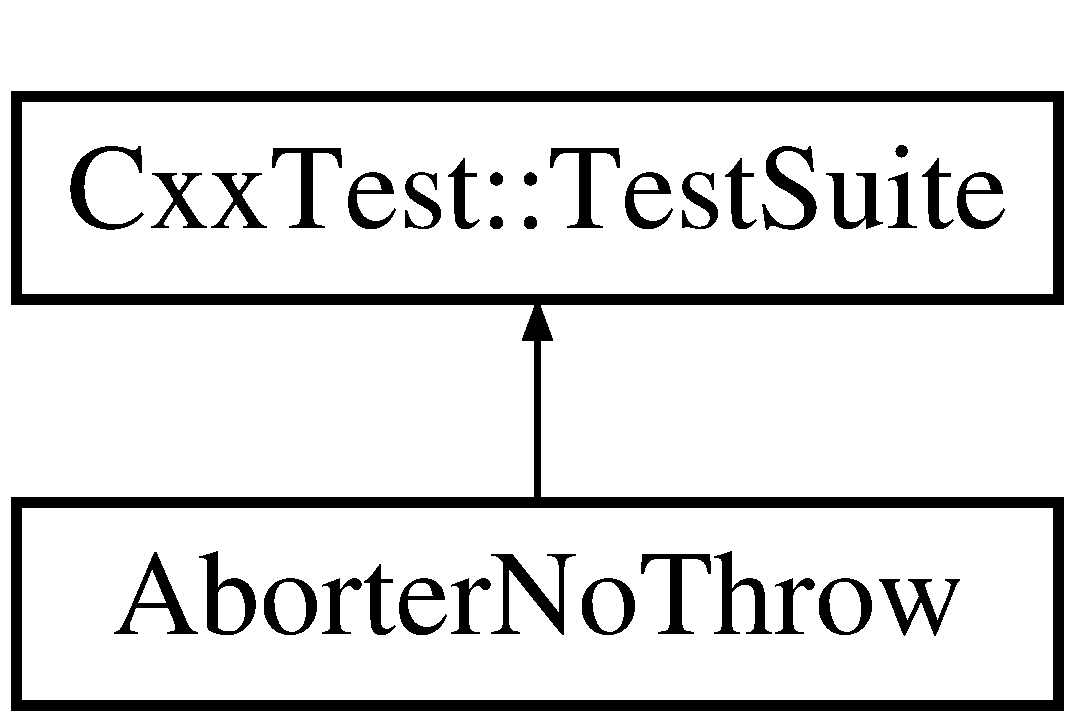
\includegraphics[height=2.000000cm]{classAborterNoThrow}
\end{center}
\end{figure}
\subsection*{Public Member Functions}
\begin{DoxyCompactItemize}
\item 
\hypertarget{classAborterNoThrow_a7abfaf7cdbde6d2858e060b44f0a1583}{void {\bfseries test\-Failures} ()}\label{classAborterNoThrow_a7abfaf7cdbde6d2858e060b44f0a1583}

\end{DoxyCompactItemize}


The documentation for this class was generated from the following file\-:\begin{DoxyCompactItemize}
\item 
test/cxxtest/test/Aborter\-No\-Throw.\-h\end{DoxyCompactItemize}

\hypertarget{classCxxTest_1_1AbortTest}{\section{Cxx\-Test\-:\-:Abort\-Test Class Reference}
\label{classCxxTest_1_1AbortTest}\index{Cxx\-Test\-::\-Abort\-Test@{Cxx\-Test\-::\-Abort\-Test}}
}


The documentation for this class was generated from the following file\-:\begin{DoxyCompactItemize}
\item 
test/cxxtest/cxxtest/Test\-Suite.\-h\end{DoxyCompactItemize}

\hypertarget{classArcball}{\section{Arcball Class Reference}
\label{classArcball}\index{Arcball@{Arcball}}
}
\subsection*{Public Member Functions}
\begin{DoxyCompactItemize}
\item 
\hypertarget{classArcball_a6e87bc32b08b572898cbc39741840b08}{{\bfseries Arcball} (\hyperlink{classmat4}{mat4} $\ast$mtx)}\label{classArcball_a6e87bc32b08b572898cbc39741840b08}

\item 
\hypertarget{classArcball_a3eeaf68e1983e08a53ae1f939aaab998}{{\bfseries Arcball} (const \hyperlink{classvec2}{vec2} \&center, float radius)}\label{classArcball_a3eeaf68e1983e08a53ae1f939aaab998}

\item 
\hypertarget{classArcball_a88a31d0e9b94ec8640d350f6645f3678}{void {\bfseries set\-\_\-damping} (float d)}\label{classArcball_a88a31d0e9b94ec8640d350f6645f3678}

\item 
\hypertarget{classArcball_a2d4725a29ba1e6542ead0aeaf8e818d7}{void {\bfseries idle} ()}\label{classArcball_a2d4725a29ba1e6542ead0aeaf8e818d7}

\item 
\hypertarget{classArcball_af68551c34a6a63f9e3ecf7995fff82ad}{void {\bfseries mouse\-\_\-down} (int x, int y)}\label{classArcball_af68551c34a6a63f9e3ecf7995fff82ad}

\item 
\hypertarget{classArcball_aca28da4e0270a68b248a58a9605056c6}{void {\bfseries mouse\-\_\-up} ()}\label{classArcball_aca28da4e0270a68b248a58a9605056c6}

\item 
\hypertarget{classArcball_a548ddff008dfd260069329ad14c988f2}{void {\bfseries mouse\-\_\-motion} (int x, int y, int shift, int ctrl, int alt)}\label{classArcball_a548ddff008dfd260069329ad14c988f2}

\item 
\hypertarget{classArcball_ab6c81c8ebfeb0624e4f5998a8bdf4d93}{void {\bfseries mouse\-\_\-motion} (int x, int y)}\label{classArcball_ab6c81c8ebfeb0624e4f5998a8bdf4d93}

\item 
\hypertarget{classArcball_a9217b887f7995b0c2c4bb4aaca2724e7}{void {\bfseries set\-\_\-constraints} (bool constrain\-\_\-x, bool constrain\-\_\-y)}\label{classArcball_a9217b887f7995b0c2c4bb4aaca2724e7}

\item 
\hypertarget{classArcball_ab92493e1a6d46098ac94858bed94cfb9}{void {\bfseries set\-\_\-params} (const \hyperlink{classvec2}{vec2} \&center, float radius)}\label{classArcball_ab92493e1a6d46098ac94858bed94cfb9}

\item 
\hypertarget{classArcball_a84c136cde1e8ee0c8ad9265e197399fb}{void {\bfseries reset\-\_\-mouse} ()}\label{classArcball_a84c136cde1e8ee0c8ad9265e197399fb}

\item 
\hypertarget{classArcball_ab3ff4548e3c265c9971929d185ca1fde}{void {\bfseries init} ()}\label{classArcball_ab3ff4548e3c265c9971929d185ca1fde}

\item 
\hypertarget{classArcball_a7d1844da5342c4b851eb4d99a7279754}{\hyperlink{classvec3}{vec3} {\bfseries constrain\-\_\-vector} (const \hyperlink{classvec3}{vec3} \&vector, const \hyperlink{classvec3}{vec3} \&axis)}\label{classArcball_a7d1844da5342c4b851eb4d99a7279754}

\item 
\hypertarget{classArcball_a500607cd1adbc27193462e2f3d2a2e7c}{\hyperlink{classvec3}{vec3} {\bfseries mouse\-\_\-to\-\_\-sphere} (const \hyperlink{classvec2}{vec2} \&p)}\label{classArcball_a500607cd1adbc27193462e2f3d2a2e7c}

\end{DoxyCompactItemize}
\subsection*{Public Attributes}
\begin{DoxyCompactItemize}
\item 
\hypertarget{classArcball_a93ef8ee8151d2e9a156ab0ef5374682a}{int {\bfseries is\-\_\-mouse\-\_\-down}}\label{classArcball_a93ef8ee8151d2e9a156ab0ef5374682a}

\item 
\hypertarget{classArcball_ae52bf983ea68ef017bfef255fb99a86a}{int {\bfseries is\-\_\-spinning}}\label{classArcball_ae52bf983ea68ef017bfef255fb99a86a}

\item 
\hypertarget{classArcball_a8e76082fc6f0b7ff54af89df070612a3}{\hyperlink{classquat}{quat} {\bfseries q\-\_\-now}}\label{classArcball_a8e76082fc6f0b7ff54af89df070612a3}

\item 
\hypertarget{classArcball_ad15ffa92fb45d16165b27d07b1133ebc}{\hyperlink{classquat}{quat} {\bfseries q\-\_\-down}}\label{classArcball_ad15ffa92fb45d16165b27d07b1133ebc}

\item 
\hypertarget{classArcball_a4d88565f2e3cdfb72eae0abc39af298e}{\hyperlink{classquat}{quat} {\bfseries q\-\_\-drag}}\label{classArcball_a4d88565f2e3cdfb72eae0abc39af298e}

\item 
\hypertarget{classArcball_a3f8c538337aba55c76b8a43f0439ba66}{\hyperlink{classquat}{quat} {\bfseries q\-\_\-increment}}\label{classArcball_a3f8c538337aba55c76b8a43f0439ba66}

\item 
\hypertarget{classArcball_ad010a1267e3d53f9c271d4c0d0240015}{\hyperlink{classvec2}{vec2} {\bfseries down\-\_\-pt}}\label{classArcball_ad010a1267e3d53f9c271d4c0d0240015}

\item 
\hypertarget{classArcball_ae948272e14633ab8df49fde0a1e048c3}{\hyperlink{classmat4}{mat4} {\bfseries rot}}\label{classArcball_ae948272e14633ab8df49fde0a1e048c3}

\item 
\hypertarget{classArcball_a7064ede24990ce3d97f3cc04da9c51db}{\hyperlink{classmat4}{mat4} {\bfseries rot\-\_\-increment}}\label{classArcball_a7064ede24990ce3d97f3cc04da9c51db}

\item 
\hypertarget{classArcball_ace75589d343d73148ca3e97de2fc4607}{\hyperlink{classmat4}{mat4} $\ast$ {\bfseries rot\-\_\-ptr}}\label{classArcball_ace75589d343d73148ca3e97de2fc4607}

\item 
\hypertarget{classArcball_aaeed50eff2338720a5ccc6530e28e941}{bool {\bfseries constraint\-\_\-x}}\label{classArcball_aaeed50eff2338720a5ccc6530e28e941}

\item 
\hypertarget{classArcball_aa46718d1b438010622664c65f7412c2e}{bool {\bfseries constraint\-\_\-y}}\label{classArcball_aa46718d1b438010622664c65f7412c2e}

\item 
\hypertarget{classArcball_ac196c376b8f265704033938b0d6a7b6d}{\hyperlink{classvec2}{vec2} {\bfseries center}}\label{classArcball_ac196c376b8f265704033938b0d6a7b6d}

\item 
\hypertarget{classArcball_aed2e9c177c4f650e9aef6f3050972f6a}{float {\bfseries radius}}\label{classArcball_aed2e9c177c4f650e9aef6f3050972f6a}

\item 
\hypertarget{classArcball_a0b3b8f1e4f37e60ad3138ea41e0d0f13}{float {\bfseries damp\-\_\-factor}}\label{classArcball_a0b3b8f1e4f37e60ad3138ea41e0d0f13}

\item 
\hypertarget{classArcball_a5cb4b94f265115a4a60027071a123b8f}{int {\bfseries zero\-\_\-increment}}\label{classArcball_a5cb4b94f265115a4a60027071a123b8f}

\end{DoxyCompactItemize}


The documentation for this class was generated from the following files\-:\begin{DoxyCompactItemize}
\item 
glui/src/arcball.\-h\item 
glui/src/arcball.\-cpp\end{DoxyCompactItemize}

\hypertarget{structbacking__store__struct}{\section{backing\-\_\-store\-\_\-struct Struct Reference}
\label{structbacking__store__struct}\index{backing\-\_\-store\-\_\-struct@{backing\-\_\-store\-\_\-struct}}
}
\subsection*{Public Member Functions}
\begin{DoxyCompactItemize}
\item 
\hypertarget{structbacking__store__struct_a22c5a1f420b61a5c3f48e857d61ceb35}{{\bfseries J\-M\-E\-T\-H\-O\-D} (void, read\-\_\-backing\-\_\-store,(\hyperlink{structjpeg__common__struct}{j\-\_\-common\-\_\-ptr} cinfo, \hyperlink{structbacking__store__struct}{backing\-\_\-store\-\_\-ptr} info, void F\-A\-R $\ast$buffer\-\_\-address, long file\-\_\-offset, long byte\-\_\-count))}\label{structbacking__store__struct_a22c5a1f420b61a5c3f48e857d61ceb35}

\item 
\hypertarget{structbacking__store__struct_aa54343491f740a9d799eeb9c3e7e09d2}{{\bfseries J\-M\-E\-T\-H\-O\-D} (void, write\-\_\-backing\-\_\-store,(\hyperlink{structjpeg__common__struct}{j\-\_\-common\-\_\-ptr} cinfo, \hyperlink{structbacking__store__struct}{backing\-\_\-store\-\_\-ptr} info, void F\-A\-R $\ast$buffer\-\_\-address, long file\-\_\-offset, long byte\-\_\-count))}\label{structbacking__store__struct_aa54343491f740a9d799eeb9c3e7e09d2}

\item 
\hypertarget{structbacking__store__struct_a509740a807e120959a02d25ac245eea4}{{\bfseries J\-M\-E\-T\-H\-O\-D} (void, close\-\_\-backing\-\_\-store,(\hyperlink{structjpeg__common__struct}{j\-\_\-common\-\_\-ptr} cinfo, \hyperlink{structbacking__store__struct}{backing\-\_\-store\-\_\-ptr} info))}\label{structbacking__store__struct_a509740a807e120959a02d25ac245eea4}

\end{DoxyCompactItemize}
\subsection*{Public Attributes}
\begin{DoxyCompactItemize}
\item 
\hypertarget{structbacking__store__struct_a90903f2f62f4fe65ac65599b50d0411e}{F\-I\-L\-E $\ast$ {\bfseries temp\-\_\-file}}\label{structbacking__store__struct_a90903f2f62f4fe65ac65599b50d0411e}

\item 
\hypertarget{structbacking__store__struct_aee24b7268410bcf129e83a8e2a2f4d45}{char {\bfseries temp\-\_\-name} \mbox{[}T\-E\-M\-P\-\_\-\-N\-A\-M\-E\-\_\-\-L\-E\-N\-G\-T\-H\mbox{]}}\label{structbacking__store__struct_aee24b7268410bcf129e83a8e2a2f4d45}

\end{DoxyCompactItemize}


The documentation for this struct was generated from the following file\-:\begin{DoxyCompactItemize}
\item 
libjpeg/jmemsys.\-h\end{DoxyCompactItemize}

\hypertarget{classBadTest}{\section{Bad\-Test Class Reference}
\label{classBadTest}\index{Bad\-Test@{Bad\-Test}}
}
Inheritance diagram for Bad\-Test\-:\begin{figure}[H]
\begin{center}
\leavevmode
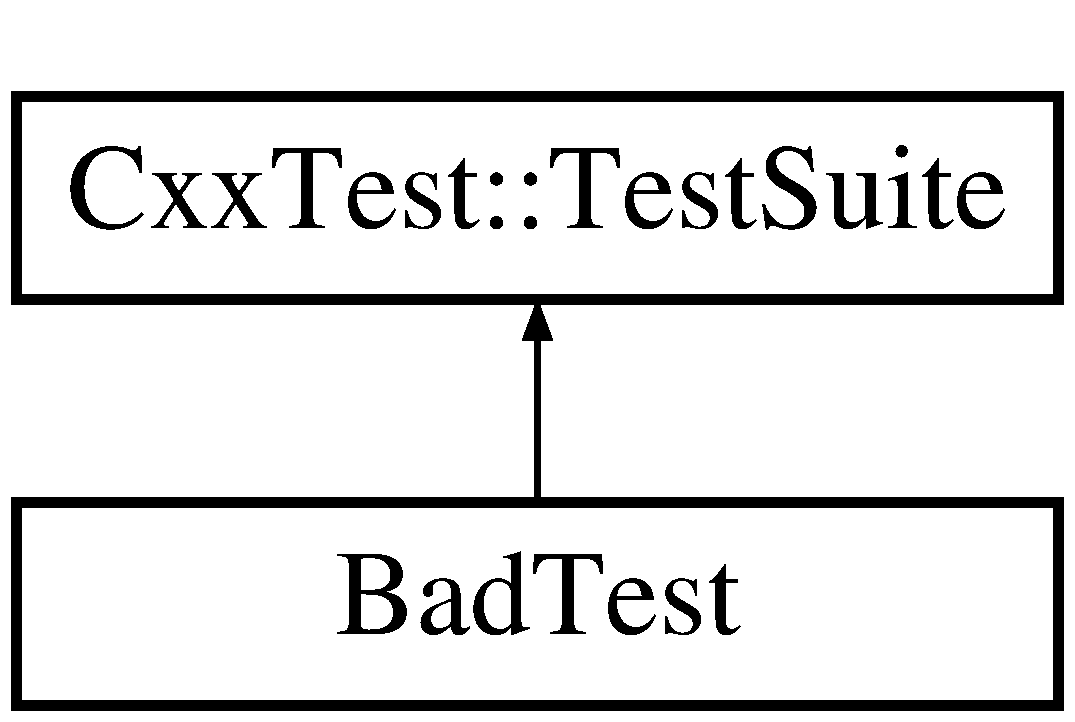
\includegraphics[height=2.000000cm]{classBadTest}
\end{center}
\end{figure}
\subsection*{Public Member Functions}
\begin{DoxyCompactItemize}
\item 
\hypertarget{classBadTest_a4b5757bbb2a54f121aa55245358b5bc6}{void {\bfseries test\-Equality} ()}\label{classBadTest_a4b5757bbb2a54f121aa55245358b5bc6}

\item 
\hypertarget{classBadTest_a535c1cbb86415ad35fc13378f75bb075}{void {\bfseries test\-Addition} ()}\label{classBadTest_a535c1cbb86415ad35fc13378f75bb075}

\item 
\hypertarget{classBadTest_a58cdf63e9c6a42259d35585afdedb6e8}{void {\bfseries Test\-Multiplication} ()}\label{classBadTest_a58cdf63e9c6a42259d35585afdedb6e8}

\item 
\hypertarget{classBadTest_ab0696b9b32488d8433eafe1e8da78ab3}{void {\bfseries test\-Comparison} ()}\label{classBadTest_ab0696b9b32488d8433eafe1e8da78ab3}

\item 
\hypertarget{classBadTest_a7eadd8682a1ea41dbf9b9ebd4930acb5}{void {\bfseries test\-The\-World\-Is\-Crazy} ()}\label{classBadTest_a7eadd8682a1ea41dbf9b9ebd4930acb5}

\item 
\hypertarget{classBadTest_a576ec735bc1935207f69b8712c506ad0}{void {\bfseries test\-\_\-\-Failure} ()}\label{classBadTest_a576ec735bc1935207f69b8712c506ad0}

\item 
\hypertarget{classBadTest_a9544f4c35e602de53443d0fe4513618d}{void {\bfseries test\-\_\-\-T\-S\-\_\-\-W\-A\-R\-N\-\_\-macro} ()}\label{classBadTest_a9544f4c35e602de53443d0fe4513618d}

\end{DoxyCompactItemize}


The documentation for this class was generated from the following file\-:\begin{DoxyCompactItemize}
\item 
test/cxxtest/test/Bad\-Test.\-h\end{DoxyCompactItemize}

\hypertarget{classBadTestSuite1}{\section{Bad\-Test\-Suite1 Class Reference}
\label{classBadTestSuite1}\index{Bad\-Test\-Suite1@{Bad\-Test\-Suite1}}
}
Inheritance diagram for Bad\-Test\-Suite1\-:\begin{figure}[H]
\begin{center}
\leavevmode
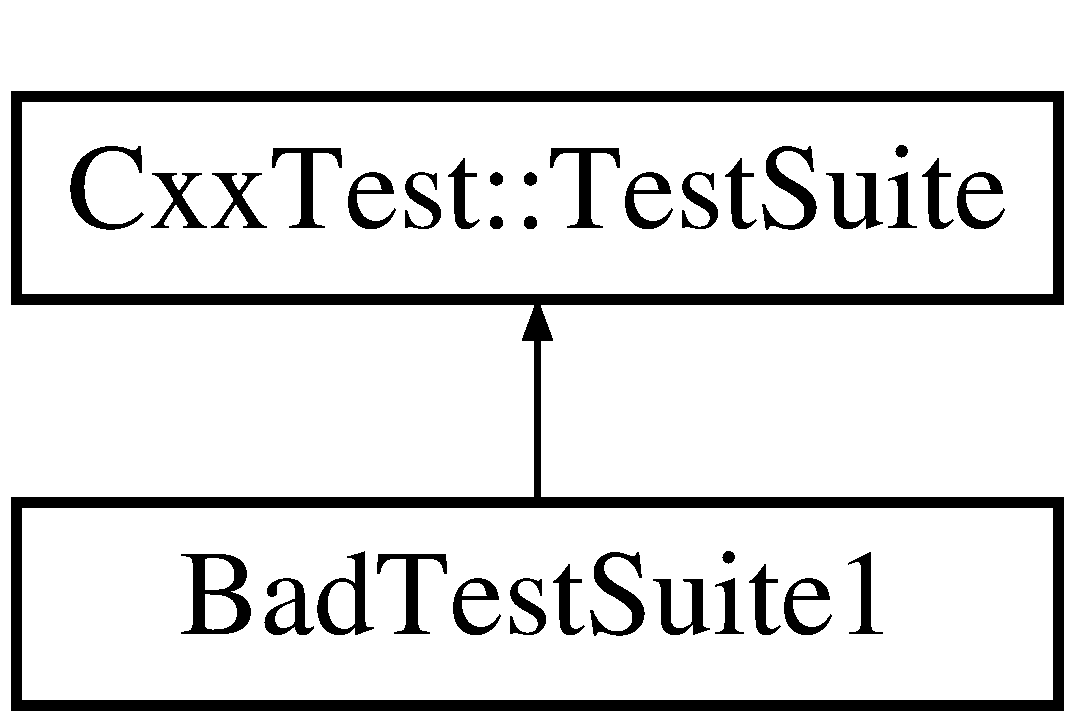
\includegraphics[height=2.000000cm]{classBadTestSuite1}
\end{center}
\end{figure}
\subsection*{Public Member Functions}
\begin{DoxyCompactItemize}
\item 
\hypertarget{classBadTestSuite1_a35526fe8f2f3b0cec303ce2b71d714c1}{void {\bfseries test\-Addition} (void)}\label{classBadTestSuite1_a35526fe8f2f3b0cec303ce2b71d714c1}

\end{DoxyCompactItemize}


The documentation for this class was generated from the following file\-:\begin{DoxyCompactItemize}
\item 
test/cxxtest/doc/examples/Bad\-Test\-Suite1.\-h\end{DoxyCompactItemize}

\hypertarget{classBarTestSuite1}{\section{Bar\-Test\-Suite1 Class Reference}
\label{classBarTestSuite1}\index{Bar\-Test\-Suite1@{Bar\-Test\-Suite1}}
}
Inheritance diagram for Bar\-Test\-Suite1\-:\begin{figure}[H]
\begin{center}
\leavevmode
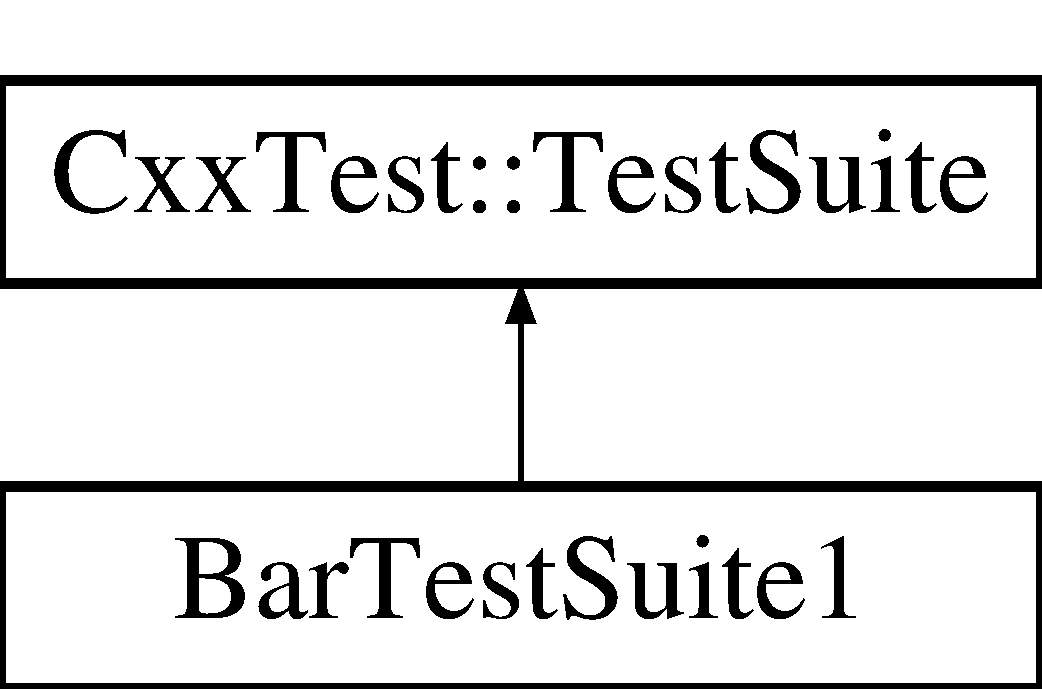
\includegraphics[height=2.000000cm]{classBarTestSuite1}
\end{center}
\end{figure}
\subsection*{Public Member Functions}
\begin{DoxyCompactItemize}
\item 
\hypertarget{classBarTestSuite1_a8d503aeca0b35c2aafc7e59be68b20df}{void {\bfseries test\-Bar} (void)}\label{classBarTestSuite1_a8d503aeca0b35c2aafc7e59be68b20df}

\end{DoxyCompactItemize}


The documentation for this class was generated from the following file\-:\begin{DoxyCompactItemize}
\item 
test/cxxtest/build\-\_\-tools/\-S\-Cons/test/libpath\-\_\-multitarget/test/test2.\-t.\-h\end{DoxyCompactItemize}

\hypertarget{classBaseGfxApp}{\section{Base\-Gfx\-App Class Reference}
\label{classBaseGfxApp}\index{Base\-Gfx\-App@{Base\-Gfx\-App}}
}


{\ttfamily \#include $<$Base\-Gfx\-App.\-h$>$}

Inheritance diagram for Base\-Gfx\-App\-:\begin{figure}[H]
\begin{center}
\leavevmode
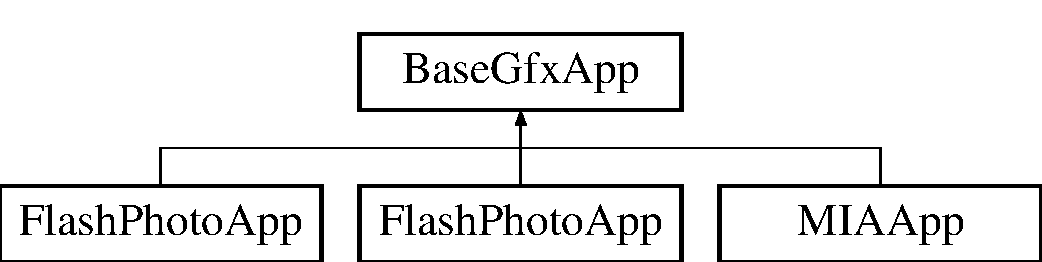
\includegraphics[height=2.000000cm]{classBaseGfxApp}
\end{center}
\end{figure}
\subsection*{Public Member Functions}
\begin{DoxyCompactItemize}
\item 
\hypertarget{classBaseGfxApp_a534a4b5293a35947fdae3805a103541d}{{\bfseries Base\-Gfx\-App} (int argc, char $\ast$argv\mbox{[}$\,$\mbox{]}, int width, int height, int x, int y, int glut\-Flags, bool create\-G\-L\-U\-I\-Win, int glui\-Win\-X, int glui\-Win\-Y)}\label{classBaseGfxApp_a534a4b5293a35947fdae3805a103541d}

\item 
\hypertarget{classBaseGfxApp_a4b3b1a475b7f2babaf1b477c34b15fb1}{void {\bfseries set\-Caption} (const std\-::string \&caption)}\label{classBaseGfxApp_a4b3b1a475b7f2babaf1b477c34b15fb1}

\item 
\hypertarget{classBaseGfxApp_a32fb420886f442d6be6b391a2ed3ecc1}{void {\bfseries set\-Window\-Dimensions} (int width, int height)}\label{classBaseGfxApp_a32fb420886f442d6be6b391a2ed3ecc1}

\item 
\hypertarget{classBaseGfxApp_acda031916c00d56c2dc901e2653e3083}{void {\bfseries run\-Main\-Loop} ()}\label{classBaseGfxApp_acda031916c00d56c2dc901e2653e3083}

\item 
\hypertarget{classBaseGfxApp_ac8de2d5a955582547af5619b771b4d6d}{virtual void {\bfseries display} ()}\label{classBaseGfxApp_ac8de2d5a955582547af5619b771b4d6d}

\item 
\hypertarget{classBaseGfxApp_a4b8d896c2fff8482553207552bc54f0a}{void {\bfseries draw\-Pixels} (int start\-\_\-x, int start\-\_\-y, int width, int height, void const $\ast$const pixels)}\label{classBaseGfxApp_a4b8d896c2fff8482553207552bc54f0a}

\item 
\hypertarget{classBaseGfxApp_a67737f7cc360b008394b1e882ed5b5d6}{virtual void {\bfseries update} (int delta\-\_\-time\-\_\-ms)}\label{classBaseGfxApp_a67737f7cc360b008394b1e882ed5b5d6}

\item 
\hypertarget{classBaseGfxApp_a0956b82d7fa58b623c498aea7073dbba}{virtual void {\bfseries mouse\-Moved} (int x, int y)}\label{classBaseGfxApp_a0956b82d7fa58b623c498aea7073dbba}

\item 
\hypertarget{classBaseGfxApp_abb23f716dd6612b3a72938e41525d338}{virtual void {\bfseries mouse\-Dragged} (int x, int y)}\label{classBaseGfxApp_abb23f716dd6612b3a72938e41525d338}

\item 
\hypertarget{classBaseGfxApp_aaaccf5a5e923a9465441a5ee712424a8}{virtual void {\bfseries left\-Mouse\-Down} (int x, int y)}\label{classBaseGfxApp_aaaccf5a5e923a9465441a5ee712424a8}

\item 
\hypertarget{classBaseGfxApp_a0a2961a932b02b2f9d7d0bb408f6fb51}{virtual void {\bfseries left\-Mouse\-Up} (int x, int y)}\label{classBaseGfxApp_a0a2961a932b02b2f9d7d0bb408f6fb51}

\item 
\hypertarget{classBaseGfxApp_afa87e6a71220945e41f0424e540125d9}{virtual void {\bfseries right\-Mouse\-Down} (int x, int y)}\label{classBaseGfxApp_afa87e6a71220945e41f0424e540125d9}

\item 
\hypertarget{classBaseGfxApp_a812643d563522a993457dd565c33f8f6}{virtual void {\bfseries right\-Mouse\-Up} (int x, int y)}\label{classBaseGfxApp_a812643d563522a993457dd565c33f8f6}

\item 
\hypertarget{classBaseGfxApp_a2c98cae9bb5ad1fb1832a6d4812670f8}{virtual void {\bfseries middle\-Mouse\-Down} (int x, int y)}\label{classBaseGfxApp_a2c98cae9bb5ad1fb1832a6d4812670f8}

\item 
\hypertarget{classBaseGfxApp_a00fc05e8d9629b72302b5adf014bdb0c}{virtual void {\bfseries middle\-Mouse\-Up} (int x, int y)}\label{classBaseGfxApp_a00fc05e8d9629b72302b5adf014bdb0c}

\item 
\hypertarget{classBaseGfxApp_a6d91e0cb7a3d48cad33956efe7eb36ca}{virtual void {\bfseries keyboard} (unsigned char c, int x, int y)}\label{classBaseGfxApp_a6d91e0cb7a3d48cad33956efe7eb36ca}

\item 
\hypertarget{classBaseGfxApp_a345566e62c9e4ec3705ec4d1c4c75f1f}{virtual void {\bfseries keyboard\-Special} (int key, int x, int y)}\label{classBaseGfxApp_a345566e62c9e4ec3705ec4d1c4c75f1f}

\item 
\hypertarget{classBaseGfxApp_acc4a40ce11edd6b6660a19cb4802a2bf}{virtual void {\bfseries keyboard\-Up} (unsigned char c, int x, int y)}\label{classBaseGfxApp_acc4a40ce11edd6b6660a19cb4802a2bf}

\item 
\hypertarget{classBaseGfxApp_afd14b435ff93b1e7f461cb8bd1a6fd59}{virtual void {\bfseries keyboard\-Special\-Up} (int key, int x, int y)}\label{classBaseGfxApp_afd14b435ff93b1e7f461cb8bd1a6fd59}

\item 
\hypertarget{classBaseGfxApp_a2978a7c358794c67df73b66776b2cef3}{virtual void {\bfseries glui\-Control} (int control\-I\-D)}\label{classBaseGfxApp_a2978a7c358794c67df73b66776b2cef3}

\item 
\hypertarget{classBaseGfxApp_a5d8d5d778a8aecd7f5f8e9c87f4c3d20}{virtual void {\bfseries reshape} (int width, int height)}\label{classBaseGfxApp_a5d8d5d778a8aecd7f5f8e9c87f4c3d20}

\item 
\hypertarget{classBaseGfxApp_ad667534069c50951121968a2027b58e2}{virtual void {\bfseries render\-One\-Frame} ()}\label{classBaseGfxApp_ad667534069c50951121968a2027b58e2}

\item 
\hypertarget{classBaseGfxApp_ace089a1a94fb6bb0bc17e1b7fa48e05d}{int {\bfseries width} () const }\label{classBaseGfxApp_ace089a1a94fb6bb0bc17e1b7fa48e05d}

\item 
\hypertarget{classBaseGfxApp_aa253dbe16a20c40e0a1bf8ff942ceea3}{int {\bfseries height} () const }\label{classBaseGfxApp_aa253dbe16a20c40e0a1bf8ff942ceea3}

\item 
\hypertarget{classBaseGfxApp_ae9779f948eff6f45beec08091e98a803}{int {\bfseries handle} ()}\label{classBaseGfxApp_ae9779f948eff6f45beec08091e98a803}

\item 
\hypertarget{classBaseGfxApp_ac721a0fedce80308c5c0e5695016e95d}{\hyperlink{classGLUI}{G\-L\-U\-I} $\ast$ {\bfseries glui} ()}\label{classBaseGfxApp_ac721a0fedce80308c5c0e5695016e95d}

\item 
\hypertarget{classBaseGfxApp_a534a4b5293a35947fdae3805a103541d}{{\bfseries Base\-Gfx\-App} (int argc, char $\ast$argv\mbox{[}$\,$\mbox{]}, int width, int height, int x, int y, int glut\-Flags, bool create\-G\-L\-U\-I\-Win, int glui\-Win\-X, int glui\-Win\-Y)}\label{classBaseGfxApp_a534a4b5293a35947fdae3805a103541d}

\item 
\hypertarget{classBaseGfxApp_a4b3b1a475b7f2babaf1b477c34b15fb1}{void {\bfseries set\-Caption} (const std\-::string \&caption)}\label{classBaseGfxApp_a4b3b1a475b7f2babaf1b477c34b15fb1}

\item 
\hypertarget{classBaseGfxApp_a32fb420886f442d6be6b391a2ed3ecc1}{void {\bfseries set\-Window\-Dimensions} (int width, int height)}\label{classBaseGfxApp_a32fb420886f442d6be6b391a2ed3ecc1}

\item 
\hypertarget{classBaseGfxApp_acda031916c00d56c2dc901e2653e3083}{void {\bfseries run\-Main\-Loop} ()}\label{classBaseGfxApp_acda031916c00d56c2dc901e2653e3083}

\item 
\hypertarget{classBaseGfxApp_ac8de2d5a955582547af5619b771b4d6d}{virtual void {\bfseries display} ()}\label{classBaseGfxApp_ac8de2d5a955582547af5619b771b4d6d}

\item 
\hypertarget{classBaseGfxApp_a4b8d896c2fff8482553207552bc54f0a}{void {\bfseries draw\-Pixels} (int start\-\_\-x, int start\-\_\-y, int width, int height, void const $\ast$const pixels)}\label{classBaseGfxApp_a4b8d896c2fff8482553207552bc54f0a}

\item 
\hypertarget{classBaseGfxApp_a67737f7cc360b008394b1e882ed5b5d6}{virtual void {\bfseries update} (int delta\-\_\-time\-\_\-ms)}\label{classBaseGfxApp_a67737f7cc360b008394b1e882ed5b5d6}

\item 
\hypertarget{classBaseGfxApp_a0956b82d7fa58b623c498aea7073dbba}{virtual void {\bfseries mouse\-Moved} (int x, int y)}\label{classBaseGfxApp_a0956b82d7fa58b623c498aea7073dbba}

\item 
\hypertarget{classBaseGfxApp_abb23f716dd6612b3a72938e41525d338}{virtual void {\bfseries mouse\-Dragged} (int x, int y)}\label{classBaseGfxApp_abb23f716dd6612b3a72938e41525d338}

\item 
\hypertarget{classBaseGfxApp_aaaccf5a5e923a9465441a5ee712424a8}{virtual void {\bfseries left\-Mouse\-Down} (int x, int y)}\label{classBaseGfxApp_aaaccf5a5e923a9465441a5ee712424a8}

\item 
\hypertarget{classBaseGfxApp_a0a2961a932b02b2f9d7d0bb408f6fb51}{virtual void {\bfseries left\-Mouse\-Up} (int x, int y)}\label{classBaseGfxApp_a0a2961a932b02b2f9d7d0bb408f6fb51}

\item 
\hypertarget{classBaseGfxApp_afa87e6a71220945e41f0424e540125d9}{virtual void {\bfseries right\-Mouse\-Down} (int x, int y)}\label{classBaseGfxApp_afa87e6a71220945e41f0424e540125d9}

\item 
\hypertarget{classBaseGfxApp_a812643d563522a993457dd565c33f8f6}{virtual void {\bfseries right\-Mouse\-Up} (int x, int y)}\label{classBaseGfxApp_a812643d563522a993457dd565c33f8f6}

\item 
\hypertarget{classBaseGfxApp_a2c98cae9bb5ad1fb1832a6d4812670f8}{virtual void {\bfseries middle\-Mouse\-Down} (int x, int y)}\label{classBaseGfxApp_a2c98cae9bb5ad1fb1832a6d4812670f8}

\item 
\hypertarget{classBaseGfxApp_a00fc05e8d9629b72302b5adf014bdb0c}{virtual void {\bfseries middle\-Mouse\-Up} (int x, int y)}\label{classBaseGfxApp_a00fc05e8d9629b72302b5adf014bdb0c}

\item 
\hypertarget{classBaseGfxApp_a6d91e0cb7a3d48cad33956efe7eb36ca}{virtual void {\bfseries keyboard} (unsigned char c, int x, int y)}\label{classBaseGfxApp_a6d91e0cb7a3d48cad33956efe7eb36ca}

\item 
\hypertarget{classBaseGfxApp_a345566e62c9e4ec3705ec4d1c4c75f1f}{virtual void {\bfseries keyboard\-Special} (int key, int x, int y)}\label{classBaseGfxApp_a345566e62c9e4ec3705ec4d1c4c75f1f}

\item 
\hypertarget{classBaseGfxApp_acc4a40ce11edd6b6660a19cb4802a2bf}{virtual void {\bfseries keyboard\-Up} (unsigned char c, int x, int y)}\label{classBaseGfxApp_acc4a40ce11edd6b6660a19cb4802a2bf}

\item 
\hypertarget{classBaseGfxApp_afd14b435ff93b1e7f461cb8bd1a6fd59}{virtual void {\bfseries keyboard\-Special\-Up} (int key, int x, int y)}\label{classBaseGfxApp_afd14b435ff93b1e7f461cb8bd1a6fd59}

\item 
\hypertarget{classBaseGfxApp_a2978a7c358794c67df73b66776b2cef3}{virtual void {\bfseries glui\-Control} (int control\-I\-D)}\label{classBaseGfxApp_a2978a7c358794c67df73b66776b2cef3}

\item 
\hypertarget{classBaseGfxApp_a89b85fe1c96fb33879cb8059649756b7}{virtual void {\bfseries reshape} (int width, int height)}\label{classBaseGfxApp_a89b85fe1c96fb33879cb8059649756b7}

\item 
\hypertarget{classBaseGfxApp_ae4177523e0853aba6e0d3ffc44ee5f33}{virtual void {\bfseries render\-One\-Frame} ()}\label{classBaseGfxApp_ae4177523e0853aba6e0d3ffc44ee5f33}

\item 
\hypertarget{classBaseGfxApp_ace089a1a94fb6bb0bc17e1b7fa48e05d}{int {\bfseries width} () const }\label{classBaseGfxApp_ace089a1a94fb6bb0bc17e1b7fa48e05d}

\item 
\hypertarget{classBaseGfxApp_aa253dbe16a20c40e0a1bf8ff942ceea3}{int {\bfseries height} () const }\label{classBaseGfxApp_aa253dbe16a20c40e0a1bf8ff942ceea3}

\item 
\hypertarget{classBaseGfxApp_ae9779f948eff6f45beec08091e98a803}{int {\bfseries handle} ()}\label{classBaseGfxApp_ae9779f948eff6f45beec08091e98a803}

\item 
\hypertarget{classBaseGfxApp_ac721a0fedce80308c5c0e5695016e95d}{\hyperlink{classGLUI}{G\-L\-U\-I} $\ast$ {\bfseries glui} ()}\label{classBaseGfxApp_ac721a0fedce80308c5c0e5695016e95d}

\end{DoxyCompactItemize}
\subsection*{Static Protected Member Functions}
\begin{DoxyCompactItemize}
\item 
\hypertarget{classBaseGfxApp_a5fe6a77d37044cbe28647ed3391bbb7a}{static void {\bfseries s\-\_\-reshape} (int width, int height)}\label{classBaseGfxApp_a5fe6a77d37044cbe28647ed3391bbb7a}

\item 
\hypertarget{classBaseGfxApp_a52edb2569227319feb68779844e7d857}{static void {\bfseries s\-\_\-keyboard} (unsigned char c, int x, int y)}\label{classBaseGfxApp_a52edb2569227319feb68779844e7d857}

\item 
\hypertarget{classBaseGfxApp_a1e8d90a4faab60300ddf2a4ea9b83115}{static void {\bfseries s\-\_\-keyboardspecial} (int key, int x, int y)}\label{classBaseGfxApp_a1e8d90a4faab60300ddf2a4ea9b83115}

\item 
\hypertarget{classBaseGfxApp_aa1ca205af9d6cee33949f2e6adf4c923}{static void {\bfseries s\-\_\-keyboardup} (unsigned char c, int x, int y)}\label{classBaseGfxApp_aa1ca205af9d6cee33949f2e6adf4c923}

\item 
\hypertarget{classBaseGfxApp_a0e4dfe006f3cc9126c1cc8ad32784f75}{static void {\bfseries s\-\_\-keyboardspecialup} (int key, int x, int y)}\label{classBaseGfxApp_a0e4dfe006f3cc9126c1cc8ad32784f75}

\item 
\hypertarget{classBaseGfxApp_a5e640f2394f7e038d0dd2b469d5c2e24}{static void {\bfseries s\-\_\-mousemotion} (int x, int y)}\label{classBaseGfxApp_a5e640f2394f7e038d0dd2b469d5c2e24}

\item 
\hypertarget{classBaseGfxApp_a22dd953bfb75add9fd0f8f2f8be535c5}{static void {\bfseries s\-\_\-mousebtn} (int b, int s, int x, int y)}\label{classBaseGfxApp_a22dd953bfb75add9fd0f8f2f8be535c5}

\item 
\hypertarget{classBaseGfxApp_a58415c6151a2a80e1fe2eaa9919a4dab}{static void {\bfseries s\-\_\-draw} ()}\label{classBaseGfxApp_a58415c6151a2a80e1fe2eaa9919a4dab}

\item 
\hypertarget{classBaseGfxApp_ad4a963321f1147d68369225ab0c7f32f}{static void {\bfseries s\-\_\-gluicallback} (int control\-I\-D)}\label{classBaseGfxApp_ad4a963321f1147d68369225ab0c7f32f}

\item 
\hypertarget{classBaseGfxApp_a272a9972092bed14572b0cff94415963}{static void {\bfseries s\-\_\-idle} ()}\label{classBaseGfxApp_a272a9972092bed14572b0cff94415963}

\item 
\hypertarget{classBaseGfxApp_a2dd5556ffa87b331cdc650cddf4ee80b}{static void {\bfseries s\-\_\-reshape} (int width, int height)}\label{classBaseGfxApp_a2dd5556ffa87b331cdc650cddf4ee80b}

\item 
\hypertarget{classBaseGfxApp_a0b1317ca2ef686d0b4703de1e0b8dc2f}{static void {\bfseries s\-\_\-keyboard} (unsigned char c, int x, int y)}\label{classBaseGfxApp_a0b1317ca2ef686d0b4703de1e0b8dc2f}

\item 
\hypertarget{classBaseGfxApp_a4049c8e6296308837c36e20b15ff260b}{static void {\bfseries s\-\_\-keyboardspecial} (int key, int x, int y)}\label{classBaseGfxApp_a4049c8e6296308837c36e20b15ff260b}

\item 
\hypertarget{classBaseGfxApp_a1c78238c53f06781276519b8865c5c27}{static void {\bfseries s\-\_\-keyboardup} (unsigned char c, int x, int y)}\label{classBaseGfxApp_a1c78238c53f06781276519b8865c5c27}

\item 
\hypertarget{classBaseGfxApp_ab3756a0b2dea80d1dccc215384f611f4}{static void {\bfseries s\-\_\-keyboardspecialup} (int key, int x, int y)}\label{classBaseGfxApp_ab3756a0b2dea80d1dccc215384f611f4}

\item 
\hypertarget{classBaseGfxApp_a21da7f2b2e2905a24aa75caeb447e0f8}{static void {\bfseries s\-\_\-mousemotion} (int x, int y)}\label{classBaseGfxApp_a21da7f2b2e2905a24aa75caeb447e0f8}

\item 
\hypertarget{classBaseGfxApp_a6f32766519314c08dff47d2e4fed2072}{static void {\bfseries s\-\_\-mousebtn} (int b, int s, int x, int y)}\label{classBaseGfxApp_a6f32766519314c08dff47d2e4fed2072}

\item 
\hypertarget{classBaseGfxApp_a5e0a34041334caa5f9574a2357fc435b}{static void {\bfseries s\-\_\-draw} ()}\label{classBaseGfxApp_a5e0a34041334caa5f9574a2357fc435b}

\item 
\hypertarget{classBaseGfxApp_afd45ac8877eba24c7bf873b6b53af860}{static void {\bfseries s\-\_\-gluicallback} (int control\-I\-D)}\label{classBaseGfxApp_afd45ac8877eba24c7bf873b6b53af860}

\item 
\hypertarget{classBaseGfxApp_aabe2e037dbb7659c80113d54b5684873}{static void {\bfseries s\-\_\-idle} ()}\label{classBaseGfxApp_aabe2e037dbb7659c80113d54b5684873}

\end{DoxyCompactItemize}
\subsection*{Protected Attributes}
\begin{DoxyCompactItemize}
\item 
\hypertarget{classBaseGfxApp_ad8697d6fdd10e6f336c3a662016b4fa7}{int {\bfseries m\-\_\-glut\-Window\-Handle}}\label{classBaseGfxApp_ad8697d6fdd10e6f336c3a662016b4fa7}

\item 
\hypertarget{classBaseGfxApp_a1435ba2e22c8f5897964b24e988da18d}{\hyperlink{classGLUI}{G\-L\-U\-I} $\ast$ {\bfseries m\-\_\-glui}}\label{classBaseGfxApp_a1435ba2e22c8f5897964b24e988da18d}

\item 
\hypertarget{classBaseGfxApp_a2e70a389224f8affe7c137f7e20dc8c1}{bool {\bfseries m\-\_\-drag}}\label{classBaseGfxApp_a2e70a389224f8affe7c137f7e20dc8c1}

\item 
\hypertarget{classBaseGfxApp_a7e5ef1c8f25fe081b4a1fd4ce6a96e07}{int {\bfseries m\-\_\-width}}\label{classBaseGfxApp_a7e5ef1c8f25fe081b4a1fd4ce6a96e07}

\item 
\hypertarget{classBaseGfxApp_ac078e4fc20b5c2fe0c744966b850b412}{int {\bfseries m\-\_\-height}}\label{classBaseGfxApp_ac078e4fc20b5c2fe0c744966b850b412}

\item 
\hypertarget{classBaseGfxApp_a72e7753eb311a758240ef4998e7130c8}{int {\bfseries m\-\_\-milliseconds}}\label{classBaseGfxApp_a72e7753eb311a758240ef4998e7130c8}

\end{DoxyCompactItemize}
\subsection*{Static Protected Attributes}
\begin{DoxyCompactItemize}
\item 
\hypertarget{classBaseGfxApp_a9ef4c8189639df51e80ee8032d80237d}{static \hyperlink{classBaseGfxApp}{Base\-Gfx\-App} $\ast$ {\bfseries s\-\_\-current\-App} = N\-U\-L\-L}\label{classBaseGfxApp_a9ef4c8189639df51e80ee8032d80237d}

\item 
\hypertarget{classBaseGfxApp_a8f766269d3909328d3c630f0fc579665}{static bool {\bfseries s\-\_\-glut\-Initialized} = false}\label{classBaseGfxApp_a8f766269d3909328d3c630f0fc579665}

\end{DoxyCompactItemize}


\subsection{Detailed Description}
This is a base class for graphics applications built on top of the G\-L\-U\-T and \hyperlink{classGLUI}{G\-L\-U\-I} toolkits. G\-L\-U\-T and \hyperlink{classGLUI}{G\-L\-U\-I} are C libraries, so one function of this class is to wrap the funcationality they provide in a class structure that lends itself to C++. To receive callbaks from G\-L\-U\-T and \hyperlink{classGLUI}{G\-L\-U\-I} that allow you to render graphics and respond to user interface events, simply override the virtual methods in this class within your own subclass. 

The documentation for this class was generated from the following files\-:\begin{DoxyCompactItemize}
\item 
libphoto/Base\-Gfx\-App.\-h\item 
libphoto/Base\-Gfx\-App.\-cpp\end{DoxyCompactItemize}

\hypertarget{classBaseTests}{\section{Base\-Tests Class Reference}
\label{classBaseTests}\index{Base\-Tests@{Base\-Tests}}
}
Inheritance diagram for Base\-Tests\-:\begin{figure}[H]
\begin{center}
\leavevmode
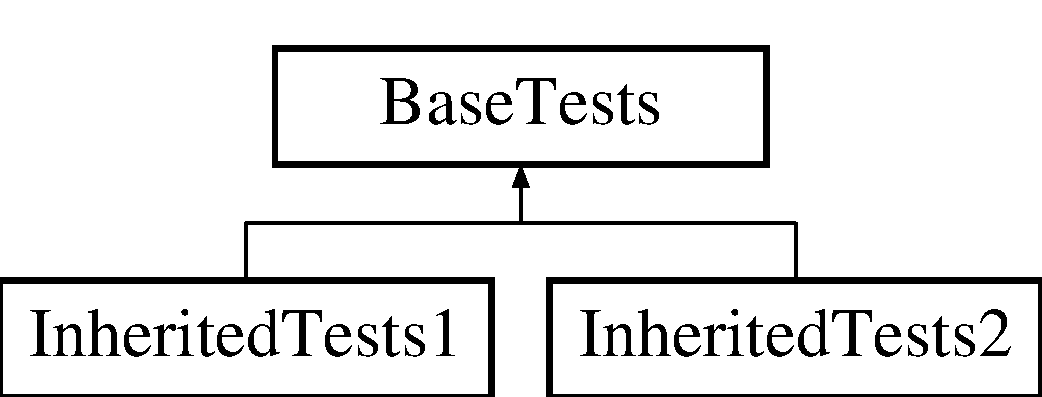
\includegraphics[height=2.000000cm]{classBaseTests}
\end{center}
\end{figure}
\subsection*{Public Member Functions}
\begin{DoxyCompactItemize}
\item 
\hypertarget{classBaseTests_aec13d99194f22f36cc61f6c0fa407fe8}{void {\bfseries test\-Equality} ()}\label{classBaseTests_aec13d99194f22f36cc61f6c0fa407fe8}

\item 
\hypertarget{classBaseTests_a8ce8ad83797fb9d7472509be6c5c67eb}{void {\bfseries test\-Addition} ()}\label{classBaseTests_a8ce8ad83797fb9d7472509be6c5c67eb}

\item 
\hypertarget{classBaseTests_aa39f9262676845274eddb1c210abf656}{void {\bfseries Test\-Multiplication} ()}\label{classBaseTests_aa39f9262676845274eddb1c210abf656}

\item 
\hypertarget{classBaseTests_ab67a5019ea16c60b70b97b1b47e46770}{void {\bfseries test\-Comparison} ()}\label{classBaseTests_ab67a5019ea16c60b70b97b1b47e46770}

\item 
\hypertarget{classBaseTests_a8b552023860f28403e31f46326377b33}{void {\bfseries test\-The\-World\-Is\-Crazy} ()}\label{classBaseTests_a8b552023860f28403e31f46326377b33}

\item 
\hypertarget{classBaseTests_a0d987da5ef5476c4fb58047698f3ecdd}{void {\bfseries test\-\_\-\-Failure} ()}\label{classBaseTests_a0d987da5ef5476c4fb58047698f3ecdd}

\item 
\hypertarget{classBaseTests_a0790e7e90128a30de493ba451ab7bdb8}{void {\bfseries test\-\_\-\-T\-S\-\_\-\-W\-A\-R\-N\-\_\-macro} ()}\label{classBaseTests_a0790e7e90128a30de493ba451ab7bdb8}

\end{DoxyCompactItemize}


The documentation for this class was generated from the following file\-:\begin{DoxyCompactItemize}
\item 
test/cxxtest/test/Inherited\-Test.\-h\end{DoxyCompactItemize}

\hypertarget{classBlur}{\section{Blur Class Reference}
\label{classBlur}\index{Blur@{Blur}}
}
Inheritance diagram for Blur\-:\begin{figure}[H]
\begin{center}
\leavevmode
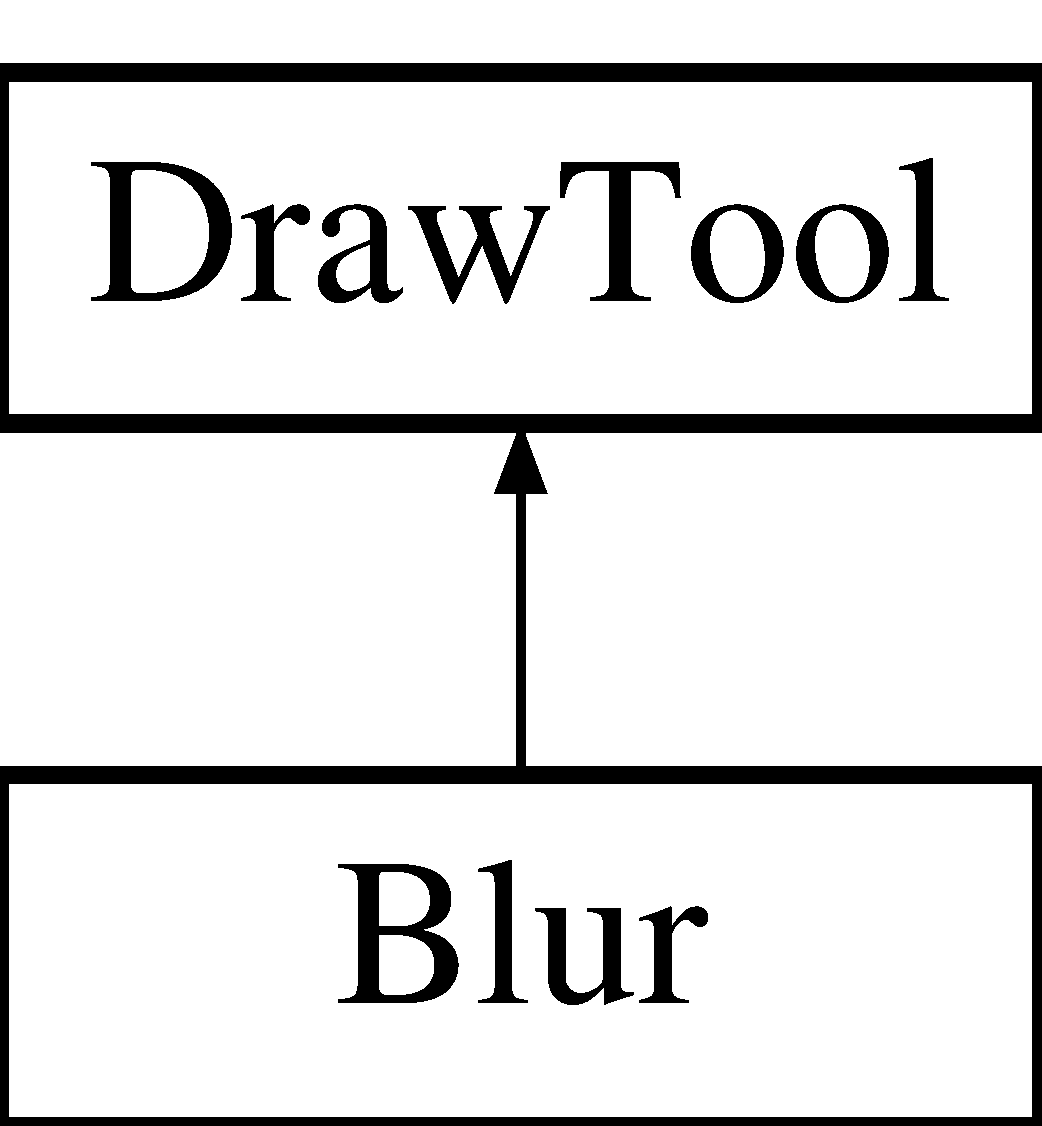
\includegraphics[height=2.000000cm]{classBlur}
\end{center}
\end{figure}
\subsection*{Public Member Functions}
\begin{DoxyCompactItemize}
\item 
\hyperlink{classBlur_a4cf976a139e3745e022c6b4fb7b18efb}{Blur} (int radius)
\item 
\hypertarget{classBlur_a6db41e9d70814abd7d188eee08779c7a}{void \hyperlink{classBlur_a6db41e9d70814abd7d188eee08779c7a}{fill\-Influence} ()}\label{classBlur_a6db41e9d70814abd7d188eee08779c7a}

\begin{DoxyCompactList}\small\item\em This creates a 2\-D matrix, the values at each index refer to the strength at which the color at that relative pixel should be applied. \end{DoxyCompactList}\item 
\hypertarget{classBlur_a74a6e5acef4b46edc5c79e909296ff53}{void \hyperlink{classBlur_a74a6e5acef4b46edc5c79e909296ff53}{apply\-Influence} (int x, int y, \hyperlink{classPixelBuffer}{Pixel\-Buffer} $\ast$buffer)}\label{classBlur_a74a6e5acef4b46edc5c79e909296ff53}

\begin{DoxyCompactList}\small\item\em This applies the influence matrix, the values at each index refer to the strength at which the color at that relative pixel should be applied. \end{DoxyCompactList}\item 
\hypertarget{classBlur_ad04ff612443d12024ae057ae757e6271}{string \hyperlink{classBlur_ad04ff612443d12024ae057ae757e6271}{get\-Name} ()}\label{classBlur_ad04ff612443d12024ae057ae757e6271}

\begin{DoxyCompactList}\small\item\em The publically viewable name the user sees. \end{DoxyCompactList}\end{DoxyCompactItemize}
\subsection*{Additional Inherited Members}


\subsection{Constructor \& Destructor Documentation}
\hypertarget{classBlur_a4cf976a139e3745e022c6b4fb7b18efb}{\index{Blur@{Blur}!Blur@{Blur}}
\index{Blur@{Blur}!Blur@{Blur}}
\subsubsection[{Blur}]{\setlength{\rightskip}{0pt plus 5cm}Blur\-::\-Blur (
\begin{DoxyParamCaption}
\item[{int}]{radius}
\end{DoxyParamCaption}
)}}\label{classBlur_a4cf976a139e3745e022c6b4fb7b18efb}
This is a base class that inherits from \hyperlink{classDrawTool}{Draw\-Tool}. This is used for the blur tool. 

The documentation for this class was generated from the following files\-:\begin{DoxyCompactItemize}
\item 
libphoto/Blur.\-h\item 
libphoto/Blur.\-cpp\end{DoxyCompactItemize}

\hypertarget{classCalligraphyPen}{\section{Calligraphy\-Pen Class Reference}
\label{classCalligraphyPen}\index{Calligraphy\-Pen@{Calligraphy\-Pen}}
}
Inheritance diagram for Calligraphy\-Pen\-:\begin{figure}[H]
\begin{center}
\leavevmode
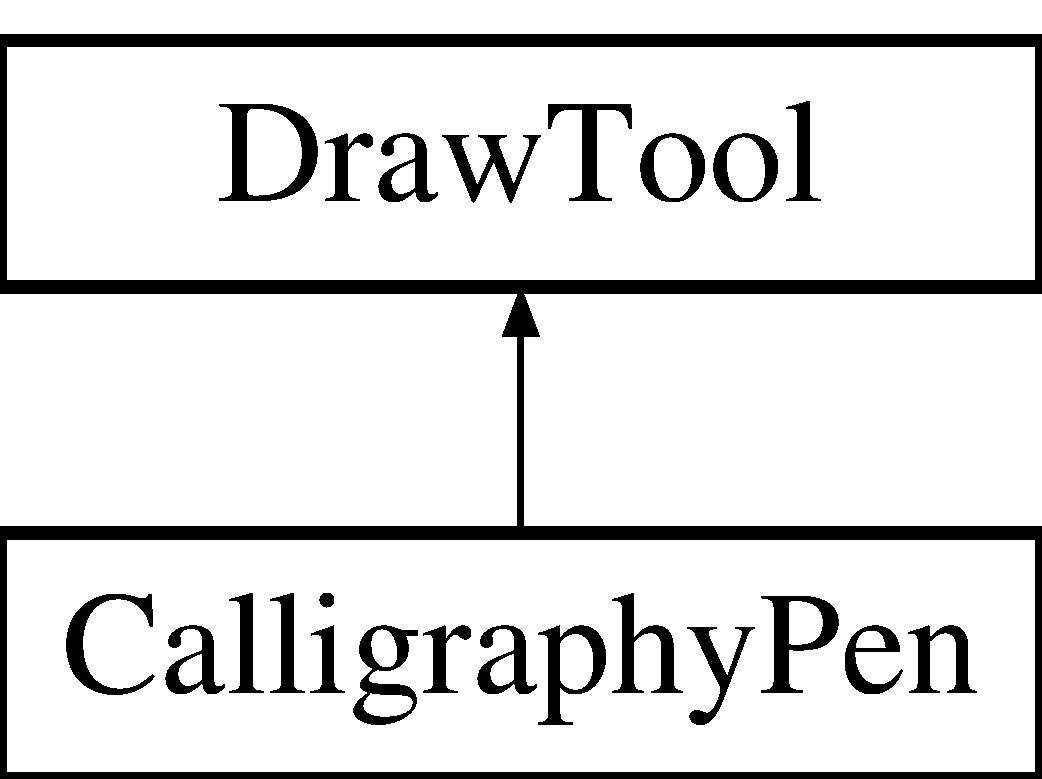
\includegraphics[height=2.000000cm]{classCalligraphyPen}
\end{center}
\end{figure}
\subsection*{Public Member Functions}
\begin{DoxyCompactItemize}
\item 
\hypertarget{classCalligraphyPen_a0a7aee1d27a037b4d863df7433530e54}{{\bfseries Calligraphy\-Pen} (\hyperlink{classColorData}{Color\-Data} $\ast$tool\-Color, int height, int width)}\label{classCalligraphyPen_a0a7aee1d27a037b4d863df7433530e54}

\item 
\hypertarget{classCalligraphyPen_add13526712abc99aad6cac69274d35ef}{void {\bfseries fill\-Influence} ()}\label{classCalligraphyPen_add13526712abc99aad6cac69274d35ef}

\item 
\hypertarget{classCalligraphyPen_a0a7aee1d27a037b4d863df7433530e54}{{\bfseries Calligraphy\-Pen} (\hyperlink{classColorData}{Color\-Data} $\ast$tool\-Color, int height, int width)}\label{classCalligraphyPen_a0a7aee1d27a037b4d863df7433530e54}

\item 
\hypertarget{classCalligraphyPen_add13526712abc99aad6cac69274d35ef}{void {\bfseries fill\-Influence} ()}\label{classCalligraphyPen_add13526712abc99aad6cac69274d35ef}

\item 
\hypertarget{classCalligraphyPen_a0a7aee1d27a037b4d863df7433530e54}{{\bfseries Calligraphy\-Pen} (\hyperlink{classColorData}{Color\-Data} $\ast$tool\-Color, int height, int width)}\label{classCalligraphyPen_a0a7aee1d27a037b4d863df7433530e54}

\item 
\hypertarget{classCalligraphyPen_add13526712abc99aad6cac69274d35ef}{void {\bfseries fill\-Influence} ()}\label{classCalligraphyPen_add13526712abc99aad6cac69274d35ef}

\end{DoxyCompactItemize}
\subsection*{Additional Inherited Members}


The documentation for this class was generated from the following files\-:\begin{DoxyCompactItemize}
\item 
libphoto/Calligraphy\-Pen.\-h\item 
libphoto/include/libphoto.\-h\item 
libphoto/Calligraphy\-Pen.\-cpp\end{DoxyCompactItemize}

\hypertarget{structcdjpeg__progress__mgr}{\section{cdjpeg\-\_\-progress\-\_\-mgr Struct Reference}
\label{structcdjpeg__progress__mgr}\index{cdjpeg\-\_\-progress\-\_\-mgr@{cdjpeg\-\_\-progress\-\_\-mgr}}
}
\subsection*{Public Attributes}
\begin{DoxyCompactItemize}
\item 
\hypertarget{structcdjpeg__progress__mgr_a6303d12ac00b08da19794945793f983f}{struct \hyperlink{structjpeg__progress__mgr}{jpeg\-\_\-progress\-\_\-mgr} {\bfseries pub}}\label{structcdjpeg__progress__mgr_a6303d12ac00b08da19794945793f983f}

\item 
\hypertarget{structcdjpeg__progress__mgr_a6f5f9744a8fc43219bbb42d1757820e6}{int {\bfseries completed\-\_\-extra\-\_\-passes}}\label{structcdjpeg__progress__mgr_a6f5f9744a8fc43219bbb42d1757820e6}

\item 
\hypertarget{structcdjpeg__progress__mgr_a05c1a823d40d937b105e3ba2c13bc00d}{int {\bfseries total\-\_\-extra\-\_\-passes}}\label{structcdjpeg__progress__mgr_a05c1a823d40d937b105e3ba2c13bc00d}

\item 
\hypertarget{structcdjpeg__progress__mgr_a73fad2ed10876758edc5523d1cb10f8f}{int {\bfseries percent\-\_\-done}}\label{structcdjpeg__progress__mgr_a73fad2ed10876758edc5523d1cb10f8f}

\end{DoxyCompactItemize}


The documentation for this struct was generated from the following file\-:\begin{DoxyCompactItemize}
\item 
libjpeg/cdjpeg.\-h\end{DoxyCompactItemize}

\hypertarget{structcjpeg__source__struct}{\section{cjpeg\-\_\-source\-\_\-struct Struct Reference}
\label{structcjpeg__source__struct}\index{cjpeg\-\_\-source\-\_\-struct@{cjpeg\-\_\-source\-\_\-struct}}
}
\subsection*{Public Member Functions}
\begin{DoxyCompactItemize}
\item 
\hypertarget{structcjpeg__source__struct_a0c0027418e48e9cd566807b4c7110aa1}{{\bfseries J\-M\-E\-T\-H\-O\-D} (void, start\-\_\-input,(\hyperlink{structjpeg__compress__struct}{j\-\_\-compress\-\_\-ptr} cinfo, \hyperlink{structcjpeg__source__struct}{cjpeg\-\_\-source\-\_\-ptr} sinfo))}\label{structcjpeg__source__struct_a0c0027418e48e9cd566807b4c7110aa1}

\item 
\hypertarget{structcjpeg__source__struct_adac53dc0fdf95208d2458921ebacb93e}{{\bfseries J\-M\-E\-T\-H\-O\-D} (J\-D\-I\-M\-E\-N\-S\-I\-O\-N, get\-\_\-pixel\-\_\-rows,(\hyperlink{structjpeg__compress__struct}{j\-\_\-compress\-\_\-ptr} cinfo, \hyperlink{structcjpeg__source__struct}{cjpeg\-\_\-source\-\_\-ptr} sinfo))}\label{structcjpeg__source__struct_adac53dc0fdf95208d2458921ebacb93e}

\item 
\hypertarget{structcjpeg__source__struct_a58d0834ab3f3ed64eba2251415744b71}{{\bfseries J\-M\-E\-T\-H\-O\-D} (void, finish\-\_\-input,(\hyperlink{structjpeg__compress__struct}{j\-\_\-compress\-\_\-ptr} cinfo, \hyperlink{structcjpeg__source__struct}{cjpeg\-\_\-source\-\_\-ptr} sinfo))}\label{structcjpeg__source__struct_a58d0834ab3f3ed64eba2251415744b71}

\end{DoxyCompactItemize}
\subsection*{Public Attributes}
\begin{DoxyCompactItemize}
\item 
\hypertarget{structcjpeg__source__struct_a88d55b02438c0a3ce21422aa8578679e}{F\-I\-L\-E $\ast$ {\bfseries input\-\_\-file}}\label{structcjpeg__source__struct_a88d55b02438c0a3ce21422aa8578679e}

\item 
\hypertarget{structcjpeg__source__struct_a2ffe2e6e6af7f434f712295d1760e001}{J\-S\-A\-M\-P\-A\-R\-R\-A\-Y {\bfseries buffer}}\label{structcjpeg__source__struct_a2ffe2e6e6af7f434f712295d1760e001}

\item 
\hypertarget{structcjpeg__source__struct_a01c25aca7ac8fed165b05139aeb1f762}{J\-D\-I\-M\-E\-N\-S\-I\-O\-N {\bfseries buffer\-\_\-height}}\label{structcjpeg__source__struct_a01c25aca7ac8fed165b05139aeb1f762}

\end{DoxyCompactItemize}


The documentation for this struct was generated from the following file\-:\begin{DoxyCompactItemize}
\item 
libjpeg/cdjpeg.\-h\end{DoxyCompactItemize}

\hypertarget{classColorData}{\section{Color\-Data Class Reference}
\label{classColorData}\index{Color\-Data@{Color\-Data}}
}


{\ttfamily \#include $<$Color\-Data.\-h$>$}

\subsection*{Public Member Functions}
\begin{DoxyCompactItemize}
\item 
\hyperlink{classColorData_accf4e0c0d4549051a46783e964c95164}{Color\-Data} ()
\item 
\hypertarget{classColorData_a920b0332685ef72147fe19020fdac5d6}{{\bfseries Color\-Data} (float r, float g, float b)}\label{classColorData_a920b0332685ef72147fe19020fdac5d6}

\item 
\hypertarget{classColorData_a0ecce2c6c597d9379ebb329883298dfd}{{\bfseries Color\-Data} (float r, float g, float b, float a)}\label{classColorData_a0ecce2c6c597d9379ebb329883298dfd}

\item 
\hypertarget{classColorData_aa2e401956936f87a560b8f579514bf69}{void \hyperlink{classColorData_aa2e401956936f87a560b8f579514bf69}{set\-Red} (float r)}\label{classColorData_aa2e401956936f87a560b8f579514bf69}

\begin{DoxyCompactList}\small\item\em Set the red value of the current object. \end{DoxyCompactList}\item 
\hypertarget{classColorData_a01bbba90cac0bc1b3bd01d4aecc16477}{void \hyperlink{classColorData_a01bbba90cac0bc1b3bd01d4aecc16477}{set\-Blue} (float b)}\label{classColorData_a01bbba90cac0bc1b3bd01d4aecc16477}

\begin{DoxyCompactList}\small\item\em Set the blue value of the current object. \end{DoxyCompactList}\item 
\hypertarget{classColorData_a4a7833dfef4a33eee3857de09a72aee1}{void \hyperlink{classColorData_a4a7833dfef4a33eee3857de09a72aee1}{set\-Green} (float g)}\label{classColorData_a4a7833dfef4a33eee3857de09a72aee1}

\begin{DoxyCompactList}\small\item\em Set the green value of the current object. \end{DoxyCompactList}\item 
\hypertarget{classColorData_a547fb7bd1616e8657a825cb9a34c43c1}{void \hyperlink{classColorData_a547fb7bd1616e8657a825cb9a34c43c1}{set\-Alpha} (float a)}\label{classColorData_a547fb7bd1616e8657a825cb9a34c43c1}

\begin{DoxyCompactList}\small\item\em Set the alpha value of the current object. \end{DoxyCompactList}\item 
\hypertarget{classColorData_ab7066467c08dfad868fc4b1add70c2f2}{float \hyperlink{classColorData_ab7066467c08dfad868fc4b1add70c2f2}{get\-Red} () const }\label{classColorData_ab7066467c08dfad868fc4b1add70c2f2}

\begin{DoxyCompactList}\small\item\em Get the red value of the current object. \end{DoxyCompactList}\item 
\hypertarget{classColorData_ad9c600256c8abefdd76209fc1f68fcb5}{float \hyperlink{classColorData_ad9c600256c8abefdd76209fc1f68fcb5}{get\-Blue} () const }\label{classColorData_ad9c600256c8abefdd76209fc1f68fcb5}

\begin{DoxyCompactList}\small\item\em Get the blue value of the current object. \end{DoxyCompactList}\item 
\hypertarget{classColorData_a7e2e03b8e1e3270f33c4e4a69c00dbd6}{float \hyperlink{classColorData_a7e2e03b8e1e3270f33c4e4a69c00dbd6}{get\-Green} () const }\label{classColorData_a7e2e03b8e1e3270f33c4e4a69c00dbd6}

\begin{DoxyCompactList}\small\item\em Get the green value of the current object. \end{DoxyCompactList}\item 
\hypertarget{classColorData_a198c4490b4f1c512d2bc174418dc892a}{float {\bfseries get\-Alpha} () const }\label{classColorData_a198c4490b4f1c512d2bc174418dc892a}

\item 
\hypertarget{classColorData_ae6a0100e4e5fe7bbd00fb4defd6e4a43}{float {\bfseries get\-Luminance} () const }\label{classColorData_ae6a0100e4e5fe7bbd00fb4defd6e4a43}

\item 
\hypertarget{classColorData_a3f0f9e50c730eb653efd800070cf448c}{float {\bfseries get\-Color\-Sum} () const }\label{classColorData_a3f0f9e50c730eb653efd800070cf448c}

\item 
\hypertarget{classColorData_a5479f50514f714dc9c738a50b7b86365}{\hyperlink{classColorData}{Color\-Data} {\bfseries clamped\-Color} () const }\label{classColorData_a5479f50514f714dc9c738a50b7b86365}

\end{DoxyCompactItemize}
\subsection*{Static Private Member Functions}
\begin{DoxyCompactItemize}
\item 
\hypertarget{classColorData_a2e6ef72b4053a043ac66f3c53556b89c}{static float {\bfseries clamp\-Value} (float input, float a, float b)}\label{classColorData_a2e6ef72b4053a043ac66f3c53556b89c}

\end{DoxyCompactItemize}
\subsection*{Private Attributes}
\begin{DoxyCompactItemize}
\item 
\hypertarget{classColorData_ab085dd5021fee2698e03baf20d89bfc4}{float {\bfseries m\-\_\-red}}\label{classColorData_ab085dd5021fee2698e03baf20d89bfc4}

\item 
\hypertarget{classColorData_a594f89816d552a2cfcb91fe0ce8df2ce}{float {\bfseries m\-\_\-green}}\label{classColorData_a594f89816d552a2cfcb91fe0ce8df2ce}

\item 
\hypertarget{classColorData_a811102de4cfed5429beedcc67714520f}{float {\bfseries m\-\_\-blue}}\label{classColorData_a811102de4cfed5429beedcc67714520f}

\item 
\hypertarget{classColorData_ae8318f47f7ba2a9e2fd70b7dd03ef672}{float {\bfseries m\-\_\-alpha}}\label{classColorData_ae8318f47f7ba2a9e2fd70b7dd03ef672}

\end{DoxyCompactItemize}
\subsection*{Friends}
\begin{DoxyCompactItemize}
\item 
\hypertarget{classColorData_adf9a770243996e50282d248a4327f351}{\hyperlink{classColorData}{Color\-Data} \hyperlink{classColorData_adf9a770243996e50282d248a4327f351}{operator$\ast$} (const \hyperlink{classColorData}{Color\-Data} \&a, float f)}\label{classColorData_adf9a770243996e50282d248a4327f351}

\begin{DoxyCompactList}\small\item\em Apply component-\/wise arithmatic operations. \end{DoxyCompactList}\item 
\hypertarget{classColorData_afdc3e8e6338798779739352e6bdfa42b}{\hyperlink{classColorData}{Color\-Data} {\bfseries operator$\ast$} (const \hyperlink{classColorData}{Color\-Data} \&a, const \hyperlink{classColorData}{Color\-Data} \&b)}\label{classColorData_afdc3e8e6338798779739352e6bdfa42b}

\item 
\hypertarget{classColorData_afee00faf26189979b72f3854a17200ae}{\hyperlink{classColorData}{Color\-Data} {\bfseries operator+} (const \hyperlink{classColorData}{Color\-Data} \&a, const \hyperlink{classColorData}{Color\-Data} \&b)}\label{classColorData_afee00faf26189979b72f3854a17200ae}

\item 
\hypertarget{classColorData_a799bd54f65a61569b5b968062ac0d37e}{\hyperlink{classColorData}{Color\-Data} {\bfseries operator-\/} (const \hyperlink{classColorData}{Color\-Data} \&a, const \hyperlink{classColorData}{Color\-Data} \&b)}\label{classColorData_a799bd54f65a61569b5b968062ac0d37e}

\item 
\hypertarget{classColorData_a9dae9e77610393d100312c9d248f09cc}{bool {\bfseries operator==} (const \hyperlink{classColorData}{Color\-Data} \&a, const \hyperlink{classColorData}{Color\-Data} \&b)}\label{classColorData_a9dae9e77610393d100312c9d248f09cc}

\item 
\hypertarget{classColorData_a698ac263a286afe37e3b9ed0c5882c8c}{bool {\bfseries operator!=} (const \hyperlink{classColorData}{Color\-Data} \&a, const \hyperlink{classColorData}{Color\-Data} \&b)}\label{classColorData_a698ac263a286afe37e3b9ed0c5882c8c}

\end{DoxyCompactItemize}


\subsection{Detailed Description}
This color data class stores color in floating point format. The Red, Green, Blue, and Alpha channels range from 0.\-0 to 1.\-0. 

\subsection{Constructor \& Destructor Documentation}
\hypertarget{classColorData_accf4e0c0d4549051a46783e964c95164}{\index{Color\-Data@{Color\-Data}!Color\-Data@{Color\-Data}}
\index{Color\-Data@{Color\-Data}!ColorData@{Color\-Data}}
\subsubsection[{Color\-Data}]{\setlength{\rightskip}{0pt plus 5cm}Color\-Data\-::\-Color\-Data (
\begin{DoxyParamCaption}
{}
\end{DoxyParamCaption}
)}}\label{classColorData_accf4e0c0d4549051a46783e964c95164}
This is the color data class. Every pixel contains a colordata object detailing the r,g,b, and sometimes a values. 

The documentation for this class was generated from the following files\-:\begin{DoxyCompactItemize}
\item 
libphoto/Color\-Data.\-h\item 
libphoto/Color\-Data.\-cpp\end{DoxyCompactItemize}

\hypertarget{classComments}{\section{Comments Class Reference}
\label{classComments}\index{Comments@{Comments}}
}
Inheritance diagram for Comments\-:\begin{figure}[H]
\begin{center}
\leavevmode
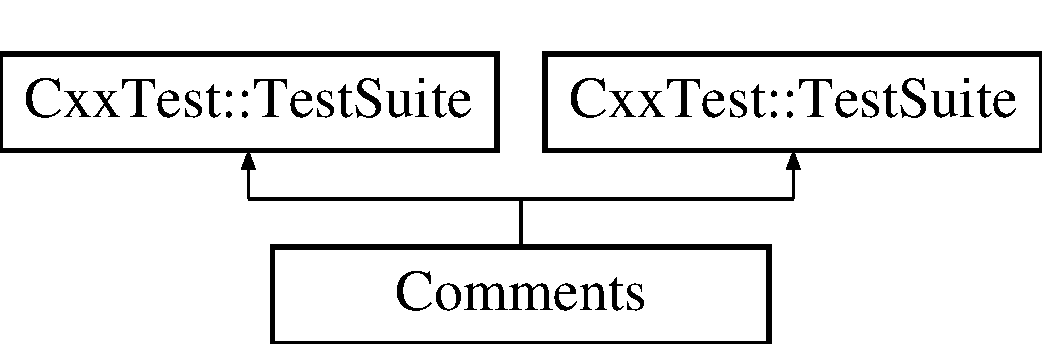
\includegraphics[height=2.000000cm]{classComments}
\end{center}
\end{figure}
\subsection*{Public Member Functions}
\begin{DoxyCompactItemize}
\item 
\hypertarget{classComments_a369157dd72693c4762e3f93e92af16d7}{void {\bfseries test\-\_\-\-Something} ()}\label{classComments_a369157dd72693c4762e3f93e92af16d7}

\item 
\hypertarget{classComments_a369157dd72693c4762e3f93e92af16d7}{void {\bfseries test\-\_\-\-Something} ()}\label{classComments_a369157dd72693c4762e3f93e92af16d7}

\end{DoxyCompactItemize}


The documentation for this class was generated from the following files\-:\begin{DoxyCompactItemize}
\item 
test/cxxtest/test/Comments.\-h\item 
test/cxxtest/test/Comments2.\-h\end{DoxyCompactItemize}

\hypertarget{classCxxTest_1_1CommonDynamicSuiteDescription}{\section{Cxx\-Test\-:\-:Common\-Dynamic\-Suite\-Description Class Reference}
\label{classCxxTest_1_1CommonDynamicSuiteDescription}\index{Cxx\-Test\-::\-Common\-Dynamic\-Suite\-Description@{Cxx\-Test\-::\-Common\-Dynamic\-Suite\-Description}}
}
Inheritance diagram for Cxx\-Test\-:\-:Common\-Dynamic\-Suite\-Description\-:\begin{figure}[H]
\begin{center}
\leavevmode
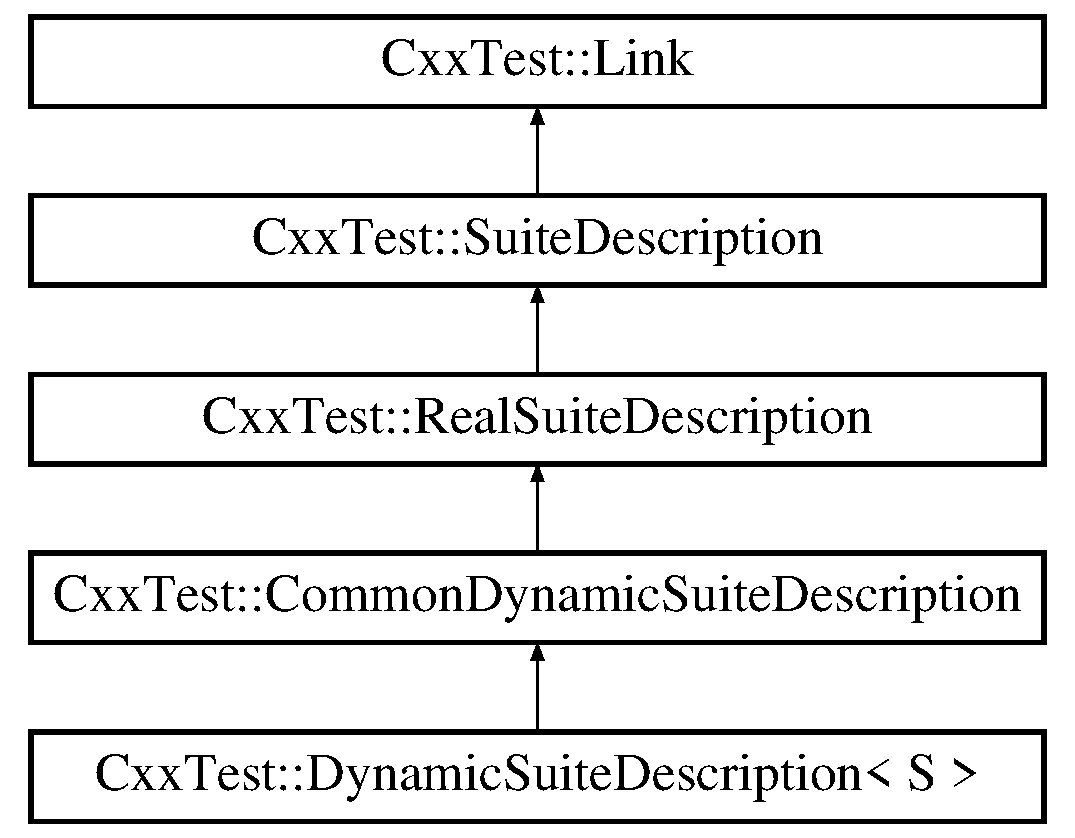
\includegraphics[height=5.000000cm]{classCxxTest_1_1CommonDynamicSuiteDescription}
\end{center}
\end{figure}
\subsection*{Public Member Functions}
\begin{DoxyCompactItemize}
\item 
\hypertarget{classCxxTest_1_1CommonDynamicSuiteDescription_a442dfefd08799d9ae046535d070f53fb}{{\bfseries Common\-Dynamic\-Suite\-Description} (const char $\ast$arg\-File, unsigned arg\-Line, const char $\ast$arg\-Suite\-Name, \hyperlink{structCxxTest_1_1List}{List} \&arg\-Tests, unsigned arg\-Create\-Line, unsigned arg\-Destroy\-Line)}\label{classCxxTest_1_1CommonDynamicSuiteDescription_a442dfefd08799d9ae046535d070f53fb}

\item 
\hypertarget{classCxxTest_1_1CommonDynamicSuiteDescription_a5a96dc7d24b2dfc45ebfc4e54eddc372}{void {\bfseries initialize} (const char $\ast$arg\-File, unsigned arg\-Line, const char $\ast$arg\-Suite\-Name, \hyperlink{structCxxTest_1_1List}{List} \&arg\-Tests, unsigned arg\-Create\-Line, unsigned arg\-Destroy\-Line)}\label{classCxxTest_1_1CommonDynamicSuiteDescription_a5a96dc7d24b2dfc45ebfc4e54eddc372}

\end{DoxyCompactItemize}
\subsection*{Protected Attributes}
\begin{DoxyCompactItemize}
\item 
\hypertarget{classCxxTest_1_1CommonDynamicSuiteDescription_a45066a52ecfbeb67b1147320a787a658}{unsigned {\bfseries \-\_\-create\-Line}}\label{classCxxTest_1_1CommonDynamicSuiteDescription_a45066a52ecfbeb67b1147320a787a658}

\item 
\hypertarget{classCxxTest_1_1CommonDynamicSuiteDescription_aec97970462595159ebe593628a3bef5a}{unsigned {\bfseries \-\_\-destroy\-Line}}\label{classCxxTest_1_1CommonDynamicSuiteDescription_aec97970462595159ebe593628a3bef5a}

\end{DoxyCompactItemize}


The documentation for this class was generated from the following files\-:\begin{DoxyCompactItemize}
\item 
test/cxxtest/cxxtest/Real\-Descriptions.\-h\item 
test/cxxtest/cxxtest/Real\-Descriptions.\-cpp\end{DoxyCompactItemize}

\hypertarget{classCppPathTest}{\section{Cpp\-Path\-Test Class Reference}
\label{classCppPathTest}\index{Cpp\-Path\-Test@{Cpp\-Path\-Test}}
}
Inheritance diagram for Cpp\-Path\-Test\-:\begin{figure}[H]
\begin{center}
\leavevmode
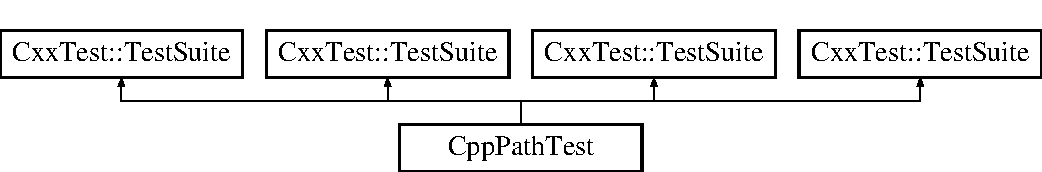
\includegraphics[height=2.000000cm]{classCppPathTest}
\end{center}
\end{figure}
\subsection*{Public Member Functions}
\begin{DoxyCompactItemize}
\item 
\hypertarget{classCppPathTest_adab4e4917cc831523ec6428ce5e4a695}{void {\bfseries test\-\_\-i\-\_\-need\-\_\-me\-\_\-exists} ()}\label{classCppPathTest_adab4e4917cc831523ec6428ce5e4a695}

\item 
\hypertarget{classCppPathTest_ac9514a3d354e7888621b93326b8ac58c}{void {\bfseries test\-\_\-i\-\_\-will\-\_\-fail} ()}\label{classCppPathTest_ac9514a3d354e7888621b93326b8ac58c}

\item 
\hypertarget{classCppPathTest_adab4e4917cc831523ec6428ce5e4a695}{void {\bfseries test\-\_\-i\-\_\-need\-\_\-me\-\_\-exists} ()}\label{classCppPathTest_adab4e4917cc831523ec6428ce5e4a695}

\item 
\hypertarget{classCppPathTest_adab4e4917cc831523ec6428ce5e4a695}{void {\bfseries test\-\_\-i\-\_\-need\-\_\-me\-\_\-exists} ()}\label{classCppPathTest_adab4e4917cc831523ec6428ce5e4a695}

\end{DoxyCompactItemize}


The documentation for this class was generated from the following files\-:\begin{DoxyCompactItemize}
\item 
test/cxxtest/build\-\_\-tools/\-S\-Cons/test/need\-\_\-cpppath/src/cpppath.\-t.\-h\item 
test/cxxtest/build\-\_\-tools/\-S\-Cons/test/printer\-\_\-propagation/src/\hyperlink{failtest_8t_8h}{failtest.\-t.\-h}\end{DoxyCompactItemize}

\hypertarget{classCrayon}{\section{Crayon Class Reference}
\label{classCrayon}\index{Crayon@{Crayon}}
}
Inheritance diagram for Crayon\-:\begin{figure}[H]
\begin{center}
\leavevmode
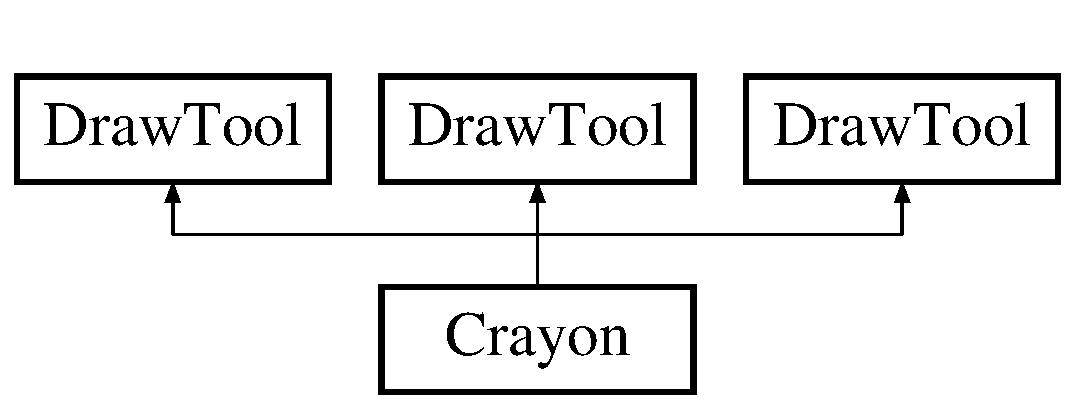
\includegraphics[height=2.000000cm]{classCrayon}
\end{center}
\end{figure}
\subsection*{Public Member Functions}
\begin{DoxyCompactItemize}
\item 
\hyperlink{classCrayon_a705e3468d3ede98a95f792bfd05be7dd}{Crayon} (\hyperlink{classColorData}{Color\-Data} $\ast$tool\-Color, int radius)
\begin{DoxyCompactList}\small\item\em For function descriptions please see the \hyperlink{classBlur}{Blur} class. \end{DoxyCompactList}\item 
void \hyperlink{classCrayon_a2af3bd14c6bc719a252a9c9f1c5eccb7}{fill\-Influence} ()
\item 
\hypertarget{classCrayon_a0484aec2b5ac3d6147e4e0bf8b3aa9d4}{string {\bfseries get\-Name} ()}\label{classCrayon_a0484aec2b5ac3d6147e4e0bf8b3aa9d4}

\end{DoxyCompactItemize}
\subsection*{Additional Inherited Members}


\subsection{Constructor \& Destructor Documentation}
\hypertarget{classCrayon_a705e3468d3ede98a95f792bfd05be7dd}{\index{Crayon@{Crayon}!Crayon@{Crayon}}
\index{Crayon@{Crayon}!Crayon@{Crayon}}
\subsubsection[{Crayon}]{\setlength{\rightskip}{0pt plus 5cm}Crayon\-::\-Crayon (
\begin{DoxyParamCaption}
\item[{{\bf Color\-Data} $\ast$}]{tool\-Color, }
\item[{int}]{radius}
\end{DoxyParamCaption}
)}}\label{classCrayon_a705e3468d3ede98a95f792bfd05be7dd}


For function descriptions please see the \hyperlink{classBlur}{Blur} class. 

This is the \hyperlink{classCrayon}{Crayon} pen class, it inherits from \hyperlink{classDrawTool}{Draw\-Tool} and is used for the \hyperlink{classCrayon}{Crayon} pen 

\subsection{Member Function Documentation}
\hypertarget{classCrayon_a2af3bd14c6bc719a252a9c9f1c5eccb7}{\index{Crayon@{Crayon}!fill\-Influence@{fill\-Influence}}
\index{fill\-Influence@{fill\-Influence}!Crayon@{Crayon}}
\subsubsection[{fill\-Influence}]{\setlength{\rightskip}{0pt plus 5cm}void Crayon\-::fill\-Influence (
\begin{DoxyParamCaption}
{}
\end{DoxyParamCaption}
)\hspace{0.3cm}{\ttfamily [virtual]}}}\label{classCrayon_a2af3bd14c6bc719a252a9c9f1c5eccb7}
Virtual function to set influence on the mask, should be overrode in sub class \par
 none \par
 void \par


Reimplemented from \hyperlink{classDrawTool_ae202bc193ba721452e81f34b6c2e6e35}{Draw\-Tool}.



The documentation for this class was generated from the following files\-:\begin{DoxyCompactItemize}
\item 
libphoto/Crayon.\-h\item 
libphoto/Crayon.\-cpp\end{DoxyCompactItemize}

\hypertarget{classCxxTest_1_1CrazyRunner}{\section{Cxx\-Test\-:\-:Crazy\-Runner Class Reference}
\label{classCxxTest_1_1CrazyRunner}\index{Cxx\-Test\-::\-Crazy\-Runner@{Cxx\-Test\-::\-Crazy\-Runner}}
}
\subsection*{Public Member Functions}
\begin{DoxyCompactItemize}
\item 
\hypertarget{classCxxTest_1_1CrazyRunner_aeb86458eba84f95c8ea4346139cd2f41}{int {\bfseries run} ()}\label{classCxxTest_1_1CrazyRunner_aeb86458eba84f95c8ea4346139cd2f41}

\item 
\hypertarget{classCxxTest_1_1CrazyRunner_a310179439335274f503d8aa43b5318db}{void {\bfseries process\-\_\-commandline} (int argc, char $\ast$$\ast$argv)}\label{classCxxTest_1_1CrazyRunner_a310179439335274f503d8aa43b5318db}

\end{DoxyCompactItemize}


The documentation for this class was generated from the following file\-:\begin{DoxyCompactItemize}
\item 
test/cxxtest/build\-\_\-tools/\-S\-Cons/test/printer\-\_\-propagation/cxxtest/Crazy\-Runner.\-h\end{DoxyCompactItemize}

\hypertarget{classCreatedTest}{\section{Created\-Test Class Reference}
\label{classCreatedTest}\index{Created\-Test@{Created\-Test}}
}
Inheritance diagram for Created\-Test\-:\begin{figure}[H]
\begin{center}
\leavevmode
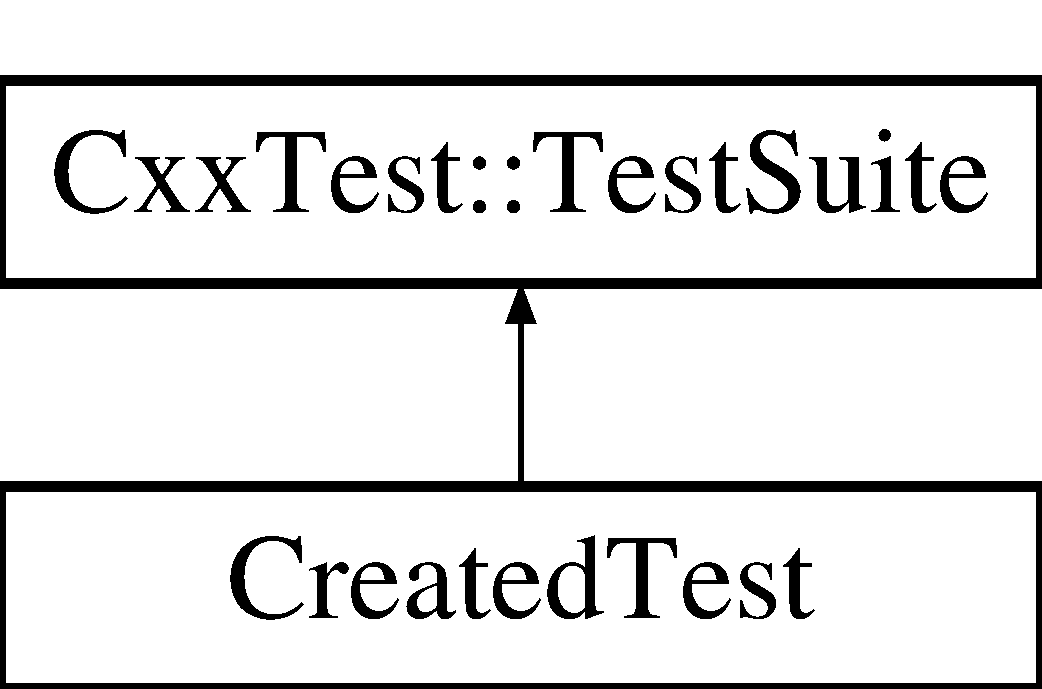
\includegraphics[height=2.000000cm]{classCreatedTest}
\end{center}
\end{figure}
\subsection*{Public Member Functions}
\begin{DoxyCompactItemize}
\item 
\hypertarget{classCreatedTest_a9ce6d9d079f3de3aab2807782179d432}{{\bfseries Created\-Test} (unsigned size)}\label{classCreatedTest_a9ce6d9d079f3de3aab2807782179d432}

\item 
\hypertarget{classCreatedTest_a47e025f3283e39f4b6ab065421ce1015}{void {\bfseries test\-\_\-nothing} ()}\label{classCreatedTest_a47e025f3283e39f4b6ab065421ce1015}

\end{DoxyCompactItemize}
\subsection*{Static Public Member Functions}
\begin{DoxyCompactItemize}
\item 
\hypertarget{classCreatedTest_a0842342004b65920648fc10a0b44cf2e}{static \hyperlink{classCreatedTest}{Created\-Test} $\ast$ {\bfseries create\-Suite} ()}\label{classCreatedTest_a0842342004b65920648fc10a0b44cf2e}

\item 
\hypertarget{classCreatedTest_aec7b74ca3ff8c6001a65a9dc13aed9ed}{static void {\bfseries destroy\-Suite} (\hyperlink{classCreatedTest}{Created\-Test} $\ast$suite)}\label{classCreatedTest_aec7b74ca3ff8c6001a65a9dc13aed9ed}

\end{DoxyCompactItemize}


The documentation for this class was generated from the following file\-:\begin{DoxyCompactItemize}
\item 
test/cxxtest/sample/Created\-Test.\-h\end{DoxyCompactItemize}

\hypertarget{structCREATESTRUCT}{\section{C\-R\-E\-A\-T\-E\-S\-T\-R\-U\-C\-T Struct Reference}
\label{structCREATESTRUCT}\index{C\-R\-E\-A\-T\-E\-S\-T\-R\-U\-C\-T@{C\-R\-E\-A\-T\-E\-S\-T\-R\-U\-C\-T}}
}
\subsection*{Public Attributes}
\begin{DoxyCompactItemize}
\item 
\hypertarget{structCREATESTRUCT_acf60cd26eeab673292e108e14d47afcf}{L\-P\-V\-O\-I\-D {\bfseries lp\-Create\-Params}}\label{structCREATESTRUCT_acf60cd26eeab673292e108e14d47afcf}

\end{DoxyCompactItemize}


The documentation for this struct was generated from the following file\-:\begin{DoxyCompactItemize}
\item 
test/cxxtest/test/fake/windows.\-h\end{DoxyCompactItemize}

\hypertarget{structMyTestSuite7_1_1Data}{\section{My\-Test\-Suite7\-:\-:Data Struct Reference}
\label{structMyTestSuite7_1_1Data}\index{My\-Test\-Suite7\-::\-Data@{My\-Test\-Suite7\-::\-Data}}
}
\subsection*{Public Member Functions}
\begin{DoxyCompactItemize}
\item 
\hypertarget{structMyTestSuite7_1_1Data_a6dedbb9d7047fb64bcbaae4da11431db}{bool {\bfseries operator==} (\hyperlink{structMyTestSuite7_1_1Data}{Data} o)}\label{structMyTestSuite7_1_1Data_a6dedbb9d7047fb64bcbaae4da11431db}

\end{DoxyCompactItemize}
\subsection*{Public Attributes}
\begin{DoxyCompactItemize}
\item 
\hypertarget{structMyTestSuite7_1_1Data_a88d7a034c6ccb4ba767ffad6b12f6b01}{char {\bfseries data} \mbox{[}3\mbox{]}}\label{structMyTestSuite7_1_1Data_a88d7a034c6ccb4ba767ffad6b12f6b01}

\end{DoxyCompactItemize}


The documentation for this struct was generated from the following file\-:\begin{DoxyCompactItemize}
\item 
test/cxxtest/doc/examples/My\-Test\-Suite7.\-h\end{DoxyCompactItemize}

\hypertarget{structMyTestSuite7_1_1Data2}{\section{My\-Test\-Suite7\-:\-:Data2 Struct Reference}
\label{structMyTestSuite7_1_1Data2}\index{My\-Test\-Suite7\-::\-Data2@{My\-Test\-Suite7\-::\-Data2}}
}
\subsection*{Public Attributes}
\begin{DoxyCompactItemize}
\item 
\hypertarget{structMyTestSuite7_1_1Data2_a052d76148d14b1a757fe078506136bb7}{char {\bfseries data} \mbox{[}3\mbox{]}}\label{structMyTestSuite7_1_1Data2_a052d76148d14b1a757fe078506136bb7}

\end{DoxyCompactItemize}


The documentation for this struct was generated from the following file\-:\begin{DoxyCompactItemize}
\item 
test/cxxtest/doc/examples/My\-Test\-Suite7.\-h\end{DoxyCompactItemize}

\hypertarget{classDeepAbort}{\section{Deep\-Abort Class Reference}
\label{classDeepAbort}\index{Deep\-Abort@{Deep\-Abort}}
}
Inheritance diagram for Deep\-Abort\-:\begin{figure}[H]
\begin{center}
\leavevmode
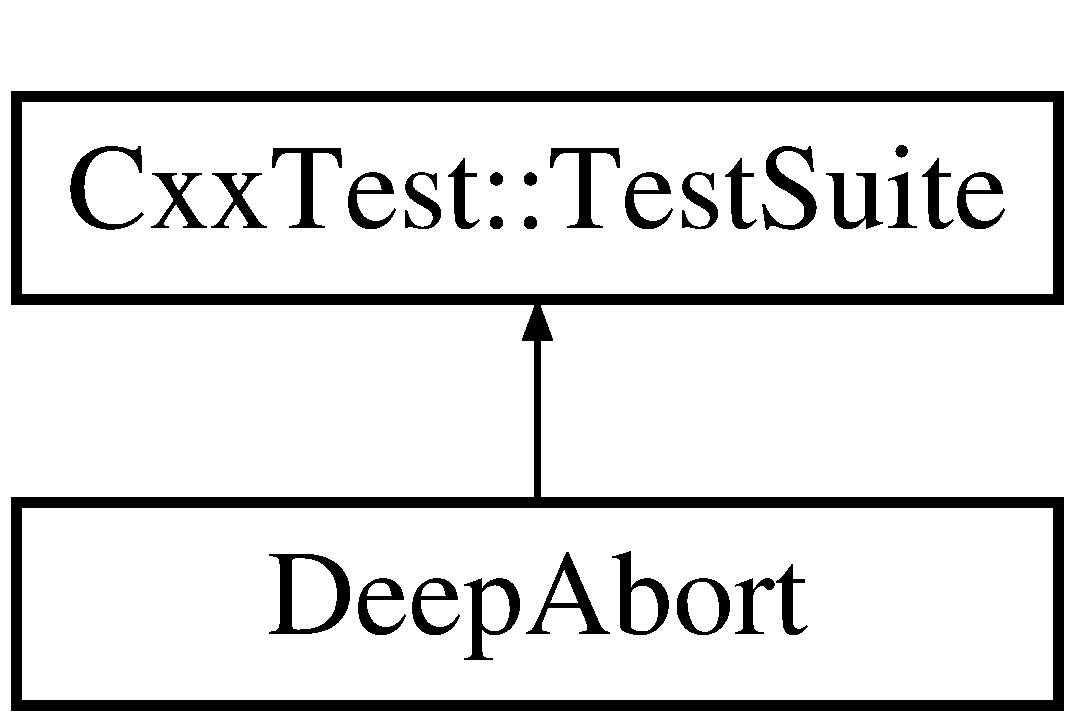
\includegraphics[height=2.000000cm]{classDeepAbort}
\end{center}
\end{figure}
\subsection*{Public Member Functions}
\begin{DoxyCompactItemize}
\item 
\hypertarget{classDeepAbort_a38a0dd26d12a7bab6949d764abd5f202}{void {\bfseries test\-Assert\-Throws\-Passes\-Abort} ()}\label{classDeepAbort_a38a0dd26d12a7bab6949d764abd5f202}

\item 
\hypertarget{classDeepAbort_a6e6e93f4e97dbf50ef5b7e7dcb75e0c2}{void {\bfseries test\-Message\-Assert\-Throws\-Passes\-Abort} ()}\label{classDeepAbort_a6e6e93f4e97dbf50ef5b7e7dcb75e0c2}

\item 
\hypertarget{classDeepAbort_a8756ae3e53fc6b727790f514ada9ace4}{void {\bfseries test\-Assert\-Throws\-Aborts} ()}\label{classDeepAbort_a8756ae3e53fc6b727790f514ada9ace4}

\item 
\hypertarget{classDeepAbort_a23530cf70d20c47f1d55a25ca54742c8}{void {\bfseries test\-Message\-Assert\-Throws\-Aborts} ()}\label{classDeepAbort_a23530cf70d20c47f1d55a25ca54742c8}

\item 
\hypertarget{classDeepAbort_ab031f15c60b2e9497348f41dff362c34}{void {\bfseries test\-Assert\-Throws\-Nothing\-Passes\-Abort} ()}\label{classDeepAbort_ab031f15c60b2e9497348f41dff362c34}

\item 
\hypertarget{classDeepAbort_a1bcacde1855a1db02028bdad32dfd7ce}{void {\bfseries test\-Message\-Assert\-Throws\-Nothing\-Passes\-Abort} ()}\label{classDeepAbort_a1bcacde1855a1db02028bdad32dfd7ce}

\item 
\hypertarget{classDeepAbort_ab9089cca8ff1e5a3884c7f9e44d0fcca}{void {\bfseries test\-Assert\-Throws\-Nothing\-Aborts} ()}\label{classDeepAbort_ab9089cca8ff1e5a3884c7f9e44d0fcca}

\item 
\hypertarget{classDeepAbort_ab236df3e2cfb517005d5087e6483ccd3}{void {\bfseries test\-Message\-Assert\-Throws\-Nothing\-Aborts} ()}\label{classDeepAbort_ab236df3e2cfb517005d5087e6483ccd3}

\item 
\hypertarget{classDeepAbort_ab5112f124fb46b8d000f4e26e5a9e01d}{void {\bfseries test\-Assert\-Throws\-Anything} ()}\label{classDeepAbort_ab5112f124fb46b8d000f4e26e5a9e01d}

\item 
\hypertarget{classDeepAbort_aa5f1304b8ccb92805b77c0cb69359883}{void {\bfseries test\-Message\-Assert\-Throws\-Anything} ()}\label{classDeepAbort_aa5f1304b8ccb92805b77c0cb69359883}

\item 
\hypertarget{classDeepAbort_a380c59fd7c24b2d439f658e6a29a9885}{void {\bfseries fail} ()}\label{classDeepAbort_a380c59fd7c24b2d439f658e6a29a9885}

\item 
\hypertarget{classDeepAbort_ae556d1c9b910303033f5178bf42ec663}{void {\bfseries throw\-Something} ()}\label{classDeepAbort_ae556d1c9b910303033f5178bf42ec663}

\item 
\hypertarget{classDeepAbort_ab69206477c9b9ae86bb494bcb9f6e974}{void {\bfseries succeed} ()}\label{classDeepAbort_ab69206477c9b9ae86bb494bcb9f6e974}

\end{DoxyCompactItemize}


The documentation for this class was generated from the following file\-:\begin{DoxyCompactItemize}
\item 
test/cxxtest/test/Deep\-Abort.\-h\end{DoxyCompactItemize}

\hypertarget{classDefaultTraits}{\section{Default\-Traits Class Reference}
\label{classDefaultTraits}\index{Default\-Traits@{Default\-Traits}}
}
Inheritance diagram for Default\-Traits\-:\begin{figure}[H]
\begin{center}
\leavevmode
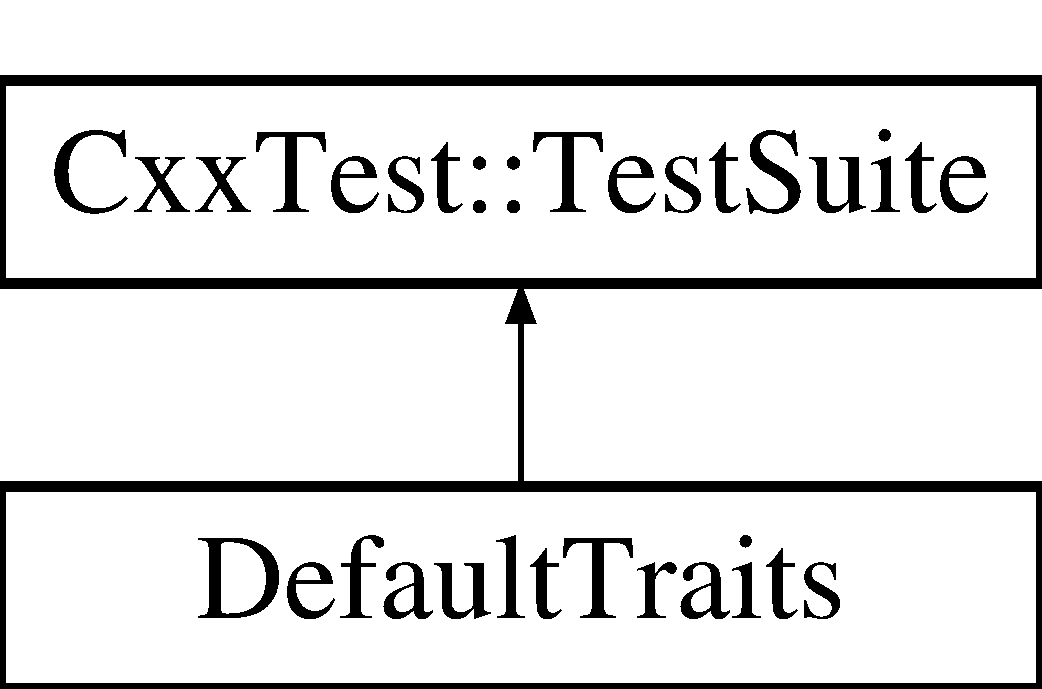
\includegraphics[height=2.000000cm]{classDefaultTraits}
\end{center}
\end{figure}
\subsection*{Classes}
\begin{DoxyCompactItemize}
\item 
struct \hyperlink{structDefaultTraits_1_1EightBytes}{Eight\-Bytes}
\item 
struct \hyperlink{structDefaultTraits_1_1NineBytes}{Nine\-Bytes}
\end{DoxyCompactItemize}
\subsection*{Public Member Functions}
\begin{DoxyCompactItemize}
\item 
\hypertarget{classDefaultTraits_a76287fe5397b049ce612c26bc16c82c9}{void {\bfseries test\-Small\-Default\-Traits} ()}\label{classDefaultTraits_a76287fe5397b049ce612c26bc16c82c9}

\item 
\hypertarget{classDefaultTraits_a12ed3f933bf5df4433ad173fb956f75b}{void {\bfseries test\-Big\-Default\-Traits} ()}\label{classDefaultTraits_a12ed3f933bf5df4433ad173fb956f75b}

\end{DoxyCompactItemize}


The documentation for this class was generated from the following file\-:\begin{DoxyCompactItemize}
\item 
test/cxxtest/test/Default\-Traits.\-h\end{DoxyCompactItemize}

\hypertarget{structCxxTest_1_1delta}{\section{Cxx\-Test\-:\-:delta$<$ X, Y, D $>$ Struct Template Reference}
\label{structCxxTest_1_1delta}\index{Cxx\-Test\-::delta$<$ X, Y, D $>$@{Cxx\-Test\-::delta$<$ X, Y, D $>$}}
}
\subsection*{Static Public Member Functions}
\begin{DoxyCompactItemize}
\item 
\hypertarget{structCxxTest_1_1delta_a3f7dd60392ed284232cd0f522486cc9b}{static bool {\bfseries test} (\hyperlink{classX}{X} x, Y y, D d)}\label{structCxxTest_1_1delta_a3f7dd60392ed284232cd0f522486cc9b}

\end{DoxyCompactItemize}


The documentation for this struct was generated from the following file\-:\begin{DoxyCompactItemize}
\item 
test/cxxtest/cxxtest/Test\-Suite.\-h\end{DoxyCompactItemize}

\hypertarget{classDeltaTest}{\section{Delta\-Test Class Reference}
\label{classDeltaTest}\index{Delta\-Test@{Delta\-Test}}
}
Inheritance diagram for Delta\-Test\-:\begin{figure}[H]
\begin{center}
\leavevmode
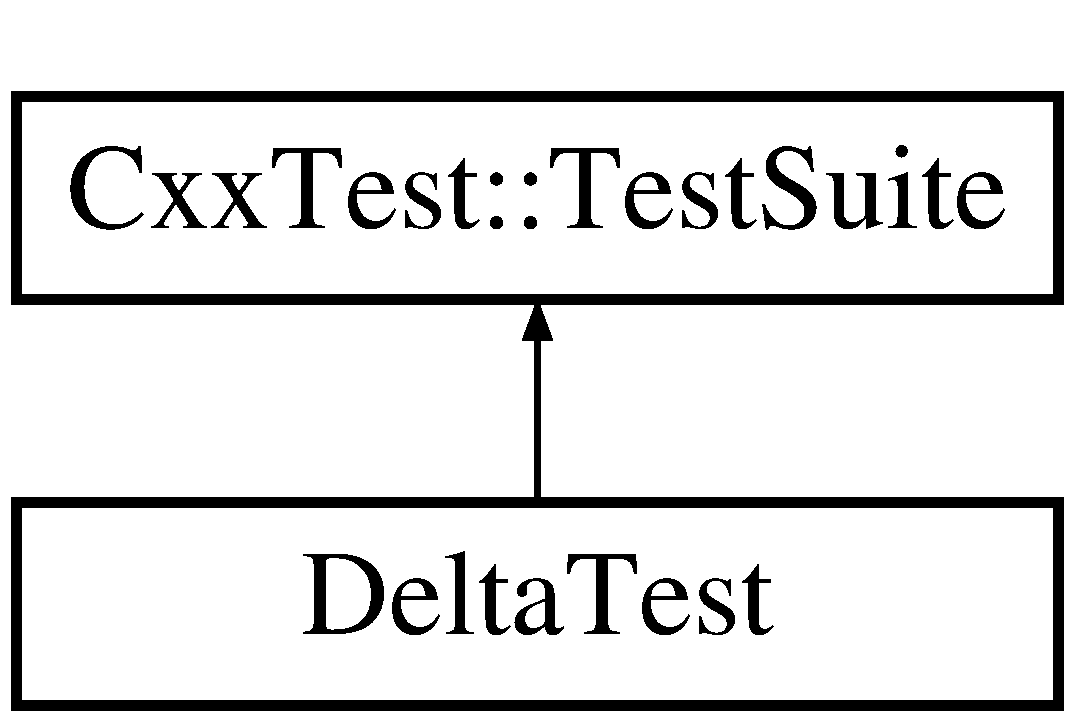
\includegraphics[height=2.000000cm]{classDeltaTest}
\end{center}
\end{figure}
\subsection*{Public Member Functions}
\begin{DoxyCompactItemize}
\item 
\hypertarget{classDeltaTest_ad18f9f106270d192a4df1e0287fbfcaa}{void {\bfseries set\-Up} ()}\label{classDeltaTest_ad18f9f106270d192a4df1e0287fbfcaa}

\item 
\hypertarget{classDeltaTest_ac0fe8b933d5f7796d6c2432b2451f0c6}{void {\bfseries test\-Sine} ()}\label{classDeltaTest_ac0fe8b933d5f7796d6c2432b2451f0c6}

\item 
\hypertarget{classDeltaTest_a166e8d778ce34a13012abc06c9e943e7}{void {\bfseries test\-Int} ()}\label{classDeltaTest_a166e8d778ce34a13012abc06c9e943e7}

\end{DoxyCompactItemize}


The documentation for this class was generated from the following file\-:\begin{DoxyCompactItemize}
\item 
test/cxxtest/sample/Delta\-Test.\-h\end{DoxyCompactItemize}

\hypertarget{classDice}{\section{Dice Class Reference}
\label{classDice}\index{Dice@{Dice}}
}
\subsection*{Public Member Functions}
\begin{DoxyCompactItemize}
\item 
\hypertarget{classDice_a33aecf673e51d0da868a1ca0b9c0b753}{unsigned {\bfseries roll} ()}\label{classDice_a33aecf673e51d0da868a1ca0b9c0b753}

\end{DoxyCompactItemize}


The documentation for this class was generated from the following files\-:\begin{DoxyCompactItemize}
\item 
test/cxxtest/sample/mock/Dice.\-h\item 
test/cxxtest/sample/mock/Dice.\-cpp\end{DoxyCompactItemize}

\hypertarget{structCxxTest_1_1differs}{\section{Cxx\-Test\-:\-:differs$<$ X, Y $>$ Struct Template Reference}
\label{structCxxTest_1_1differs}\index{Cxx\-Test\-::differs$<$ X, Y $>$@{Cxx\-Test\-::differs$<$ X, Y $>$}}
}
\subsection*{Static Public Member Functions}
\begin{DoxyCompactItemize}
\item 
\hypertarget{structCxxTest_1_1differs_a3ddb7c274892fd7232ab077c100dd09a}{static bool {\bfseries test} (\hyperlink{classX}{X} x, Y y)}\label{structCxxTest_1_1differs_a3ddb7c274892fd7232ab077c100dd09a}

\end{DoxyCompactItemize}


The documentation for this struct was generated from the following file\-:\begin{DoxyCompactItemize}
\item 
test/cxxtest/cxxtest/Test\-Suite.\-h\end{DoxyCompactItemize}

\hypertarget{structDisplay}{\section{Display Struct Reference}
\label{structDisplay}\index{Display@{Display}}
}


The documentation for this struct was generated from the following file\-:\begin{DoxyCompactItemize}
\item 
test/cxxtest/test/fake/\-X11/Xlib.\-h\end{DoxyCompactItemize}

\hypertarget{structdjpeg__dest__struct}{\section{djpeg\-\_\-dest\-\_\-struct Struct Reference}
\label{structdjpeg__dest__struct}\index{djpeg\-\_\-dest\-\_\-struct@{djpeg\-\_\-dest\-\_\-struct}}
}
\subsection*{Public Member Functions}
\begin{DoxyCompactItemize}
\item 
\hypertarget{structdjpeg__dest__struct_a387aad15333be251b9fdd4f341e3b50c}{{\bfseries J\-M\-E\-T\-H\-O\-D} (void, start\-\_\-output,(\hyperlink{structjpeg__decompress__struct}{j\-\_\-decompress\-\_\-ptr} cinfo, \hyperlink{structdjpeg__dest__struct}{djpeg\-\_\-dest\-\_\-ptr} dinfo))}\label{structdjpeg__dest__struct_a387aad15333be251b9fdd4f341e3b50c}

\item 
\hypertarget{structdjpeg__dest__struct_ab7452265598106468aeb73b63c080024}{{\bfseries J\-M\-E\-T\-H\-O\-D} (void, put\-\_\-pixel\-\_\-rows,(\hyperlink{structjpeg__decompress__struct}{j\-\_\-decompress\-\_\-ptr} cinfo, \hyperlink{structdjpeg__dest__struct}{djpeg\-\_\-dest\-\_\-ptr} dinfo, J\-D\-I\-M\-E\-N\-S\-I\-O\-N rows\-\_\-supplied))}\label{structdjpeg__dest__struct_ab7452265598106468aeb73b63c080024}

\item 
\hypertarget{structdjpeg__dest__struct_a3a1f7c965ea1dbbb577eb8902e3c893e}{{\bfseries J\-M\-E\-T\-H\-O\-D} (void, finish\-\_\-output,(\hyperlink{structjpeg__decompress__struct}{j\-\_\-decompress\-\_\-ptr} cinfo, \hyperlink{structdjpeg__dest__struct}{djpeg\-\_\-dest\-\_\-ptr} dinfo))}\label{structdjpeg__dest__struct_a3a1f7c965ea1dbbb577eb8902e3c893e}

\end{DoxyCompactItemize}
\subsection*{Public Attributes}
\begin{DoxyCompactItemize}
\item 
\hypertarget{structdjpeg__dest__struct_a5cd2d9d83c2b0b77b30169be5682d8fc}{F\-I\-L\-E $\ast$ {\bfseries output\-\_\-file}}\label{structdjpeg__dest__struct_a5cd2d9d83c2b0b77b30169be5682d8fc}

\item 
\hypertarget{structdjpeg__dest__struct_a84d1443492d9c70afae65d6f95410cf4}{J\-S\-A\-M\-P\-A\-R\-R\-A\-Y {\bfseries buffer}}\label{structdjpeg__dest__struct_a84d1443492d9c70afae65d6f95410cf4}

\item 
\hypertarget{structdjpeg__dest__struct_a78eef05ab5286600c995e9df51acf2c1}{J\-D\-I\-M\-E\-N\-S\-I\-O\-N {\bfseries buffer\-\_\-height}}\label{structdjpeg__dest__struct_a78eef05ab5286600c995e9df51acf2c1}

\end{DoxyCompactItemize}


The documentation for this struct was generated from the following file\-:\begin{DoxyCompactItemize}
\item 
libjpeg/cdjpeg.\-h\end{DoxyCompactItemize}

\hypertarget{classDoubleCall}{\section{Double\-Call Class Reference}
\label{classDoubleCall}\index{Double\-Call@{Double\-Call}}
}
Inheritance diagram for Double\-Call\-:\begin{figure}[H]
\begin{center}
\leavevmode
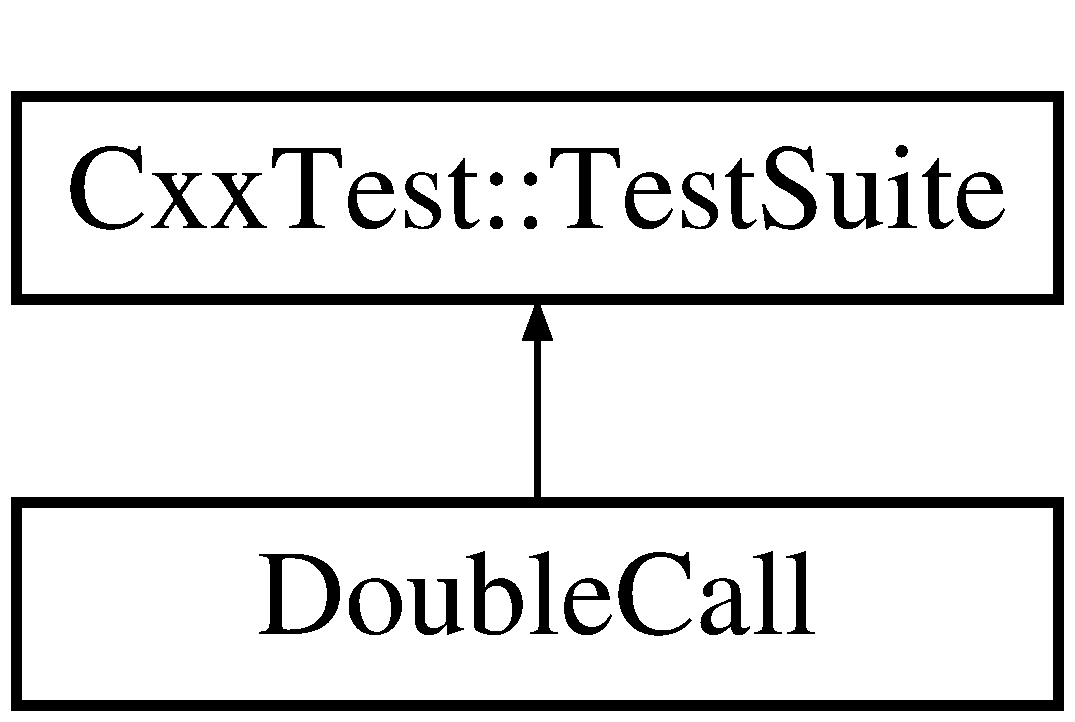
\includegraphics[height=2.000000cm]{classDoubleCall}
\end{center}
\end{figure}
\subsection*{Public Member Functions}
\begin{DoxyCompactItemize}
\item 
\hypertarget{classDoubleCall_a6bf3a9499a2d26d6779e19f8e72c6615}{void {\bfseries set\-Up} ()}\label{classDoubleCall_a6bf3a9499a2d26d6779e19f8e72c6615}

\item 
\hypertarget{classDoubleCall_a59126cc7bfbf108d1095f857a184f847}{void {\bfseries test\-Assert\-Equals\-With\-Side\-Effects} ()}\label{classDoubleCall_a59126cc7bfbf108d1095f857a184f847}

\item 
\hypertarget{classDoubleCall_a8542c7e63b1c298280f2de68880f9e3f}{void {\bfseries test\-Assert\-Differs\-With\-Side\-Effects} ()}\label{classDoubleCall_a8542c7e63b1c298280f2de68880f9e3f}

\item 
\hypertarget{classDoubleCall_a9b0f1ff26a93e7bf6aee01810e61ec17}{void {\bfseries test\-Assert\-Delta\-With\-Side\-Effects} ()}\label{classDoubleCall_a9b0f1ff26a93e7bf6aee01810e61ec17}

\item 
\hypertarget{classDoubleCall_a7090889ad0cf8435dd7426a95135bcb3}{int {\bfseries increment} ()}\label{classDoubleCall_a7090889ad0cf8435dd7426a95135bcb3}

\end{DoxyCompactItemize}
\subsection*{Public Attributes}
\begin{DoxyCompactItemize}
\item 
\hypertarget{classDoubleCall_ad258ba85647e73009f812a4f980b408c}{int {\bfseries i}}\label{classDoubleCall_ad258ba85647e73009f812a4f980b408c}

\end{DoxyCompactItemize}


The documentation for this class was generated from the following file\-:\begin{DoxyCompactItemize}
\item 
test/cxxtest/test/Double\-Call.\-h\end{DoxyCompactItemize}

\hypertarget{classDrawTool}{\section{Draw\-Tool Class Reference}
\label{classDrawTool}\index{Draw\-Tool@{Draw\-Tool}}
}
Inheritance diagram for Draw\-Tool\-:\begin{figure}[H]
\begin{center}
\leavevmode
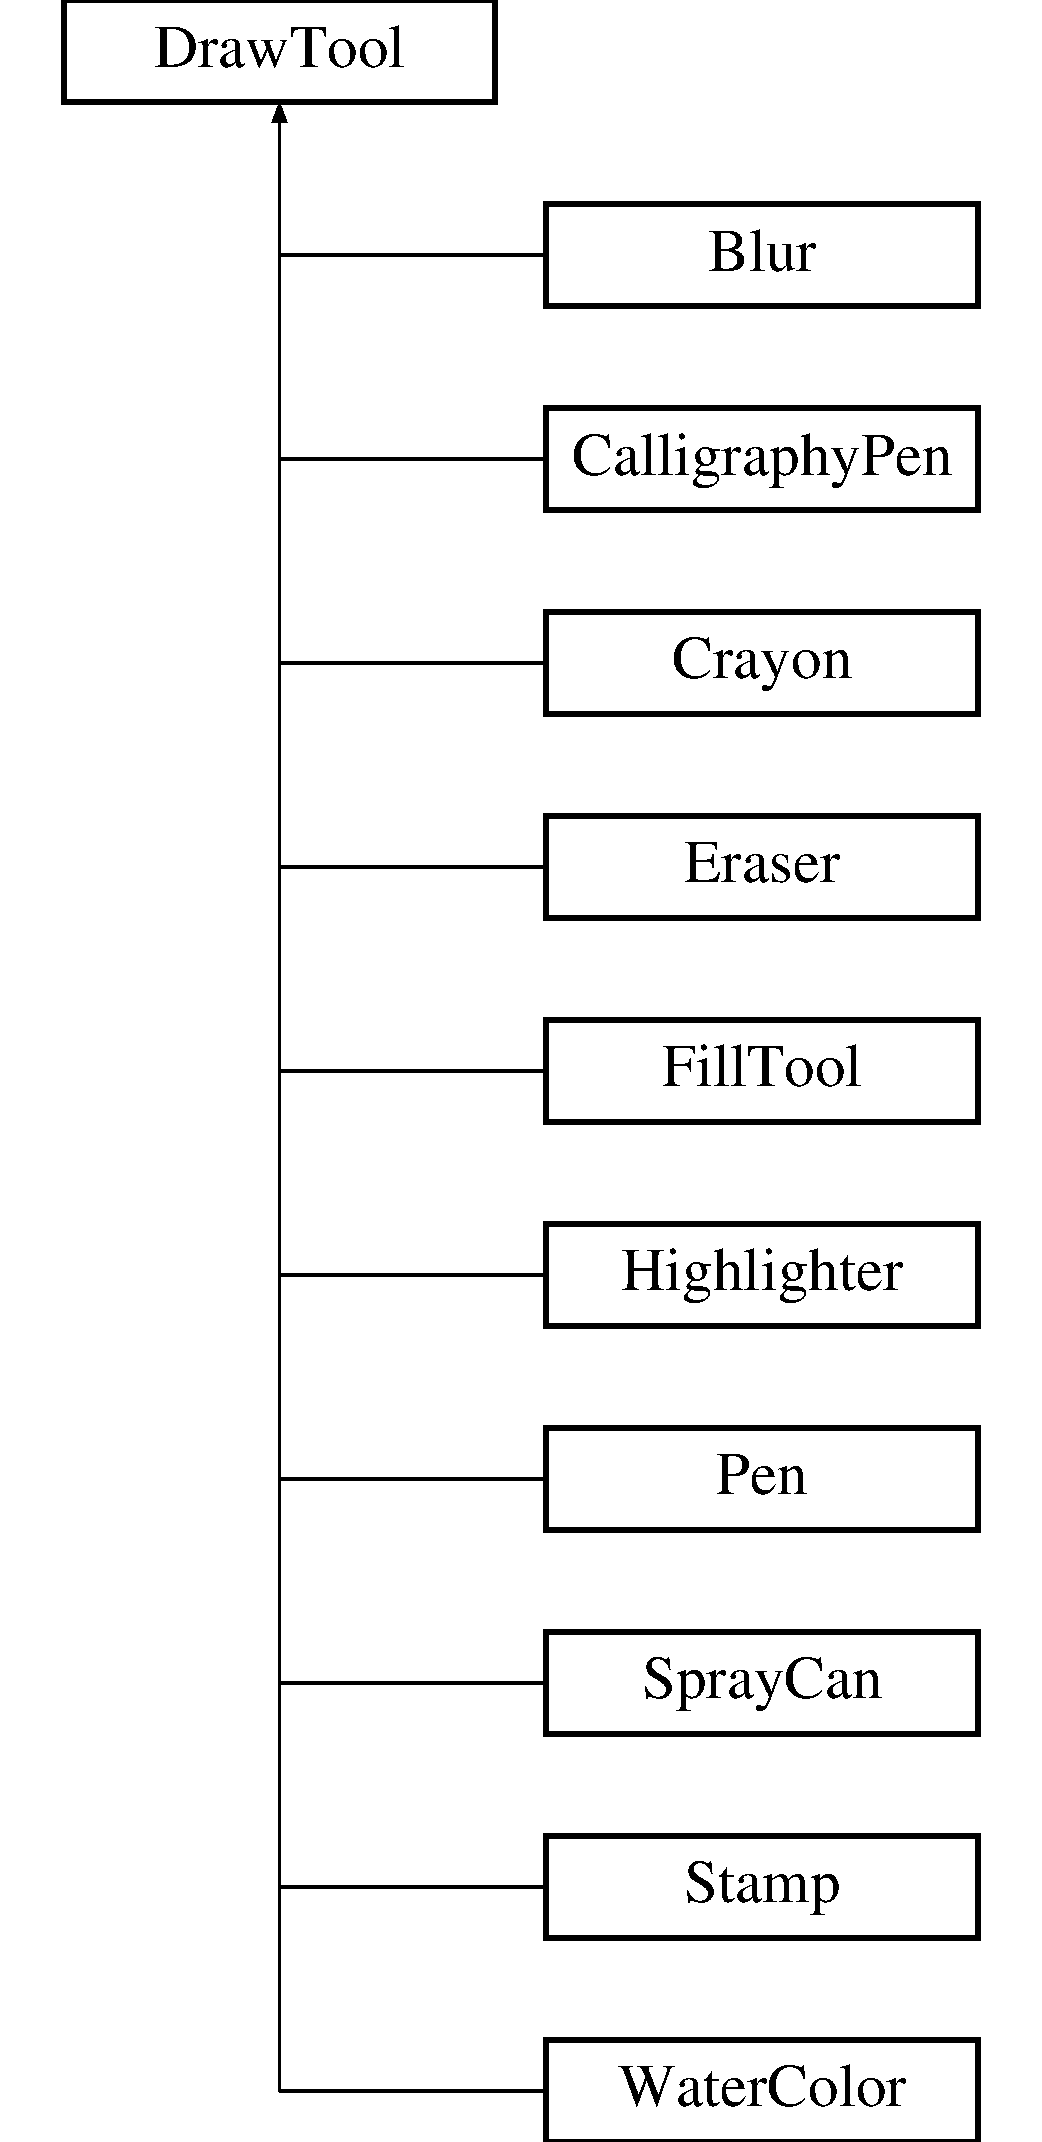
\includegraphics[height=11.000000cm]{classDrawTool}
\end{center}
\end{figure}
\subsection*{Public Member Functions}
\begin{DoxyCompactItemize}
\item 
\hypertarget{classDrawTool_aa21e3a5373ba9e4e43d6e56eec82b32d}{{\bfseries Draw\-Tool} (\hyperlink{classColorData}{Color\-Data} $\ast$tool\-Color, int width, int height)}\label{classDrawTool_aa21e3a5373ba9e4e43d6e56eec82b32d}

\item 
\hypertarget{classDrawTool_aa1816d6699a835d9c7619ee5c97be9d1}{{\bfseries Draw\-Tool} (int width, int height)}\label{classDrawTool_aa1816d6699a835d9c7619ee5c97be9d1}

\item 
\hypertarget{classDrawTool_a521ad2f183dd3354de1dd163140e8b1d}{{\bfseries Draw\-Tool} (\hyperlink{classPixelBuffer}{Pixel\-Buffer} $\ast$new\-Buffer, int width, int height)}\label{classDrawTool_a521ad2f183dd3354de1dd163140e8b1d}

\item 
\hypertarget{classDrawTool_ae202bc193ba721452e81f34b6c2e6e35}{virtual void {\bfseries fill\-Influence} ()}\label{classDrawTool_ae202bc193ba721452e81f34b6c2e6e35}

\item 
\hypertarget{classDrawTool_a65dbb2f006efc9c6053d01df75eff5a9}{virtual void {\bfseries paint} (int x, int y, int prev\-X, int prev\-Y, \hyperlink{classPixelBuffer}{Pixel\-Buffer} $\ast$buffer)}\label{classDrawTool_a65dbb2f006efc9c6053d01df75eff5a9}

\item 
\hypertarget{classDrawTool_ac60a70d91e81163d413b99382ac4255b}{virtual void {\bfseries apply\-Influence} (int x, int y, \hyperlink{classPixelBuffer}{Pixel\-Buffer} $\ast$buffer)}\label{classDrawTool_ac60a70d91e81163d413b99382ac4255b}

\item 
\hypertarget{classDrawTool_a11a450d969098c86158b6ec5f14d291e}{virtual string {\bfseries get\-Name} ()}\label{classDrawTool_a11a450d969098c86158b6ec5f14d291e}

\item 
\hypertarget{classDrawTool_ad11d4e44fcd2caf774e18ce5b2986865}{\hyperlink{classMask}{Mask} const $\ast$ {\bfseries get\-Mask} () const }\label{classDrawTool_ad11d4e44fcd2caf774e18ce5b2986865}

\item 
\hypertarget{classDrawTool_a00485271784acd5acc75840a7a17eb2e}{\hyperlink{classColorData}{Color\-Data} const $\ast$ {\bfseries get\-Tool\-Color} () const }\label{classDrawTool_a00485271784acd5acc75840a7a17eb2e}

\item 
\hypertarget{classDrawTool_a7f7097be5f6beb7b3f6ce437785cac7a}{void {\bfseries set\-Tool\-Color} (\hyperlink{classColorData}{Color\-Data} $\ast$color)}\label{classDrawTool_a7f7097be5f6beb7b3f6ce437785cac7a}

\item 
\hypertarget{classDrawTool_a04f57381cb6c71d90a66e905b46f424c}{void {\bfseries printf\-Influence} ()}\label{classDrawTool_a04f57381cb6c71d90a66e905b46f424c}

\end{DoxyCompactItemize}
\subsection*{Public Attributes}
\begin{DoxyCompactItemize}
\item 
\hypertarget{classDrawTool_a87f991a7c84a4c5ad60ebbfd813a3ab2}{bool {\bfseries allow\-Drag}}\label{classDrawTool_a87f991a7c84a4c5ad60ebbfd813a3ab2}

\end{DoxyCompactItemize}
\subsection*{Protected Attributes}
\begin{DoxyCompactItemize}
\item 
\hypertarget{classDrawTool_a0a3cc5165047f1158bff38750ddf8e85}{\hyperlink{classMask}{Mask} $\ast$ {\bfseries m\-\_\-mask}}\label{classDrawTool_a0a3cc5165047f1158bff38750ddf8e85}

\item 
\hypertarget{classDrawTool_a3bb9153560d2b084c56d5e7d749d49a2}{\hyperlink{classColorData}{Color\-Data} $\ast$ {\bfseries m\-\_\-tool\-Color}}\label{classDrawTool_a3bb9153560d2b084c56d5e7d749d49a2}

\item 
\hypertarget{classDrawTool_a917dfe1261ea0d5c4250f8b83eddb177}{\hyperlink{classPixelBuffer}{Pixel\-Buffer} $\ast$ {\bfseries image\-Buffer}}\label{classDrawTool_a917dfe1261ea0d5c4250f8b83eddb177}

\end{DoxyCompactItemize}


The documentation for this class was generated from the following files\-:\begin{DoxyCompactItemize}
\item 
libphoto/Drawtool.\-h\item 
libphoto/Drawtool.\-cpp\end{DoxyCompactItemize}

\hypertarget{classCxxTest_1_1DummyGui}{\section{Cxx\-Test\-:\-:Dummy\-Gui Class Reference}
\label{classCxxTest_1_1DummyGui}\index{Cxx\-Test\-::\-Dummy\-Gui@{Cxx\-Test\-::\-Dummy\-Gui}}
}
Inheritance diagram for Cxx\-Test\-:\-:Dummy\-Gui\-:\begin{figure}[H]
\begin{center}
\leavevmode
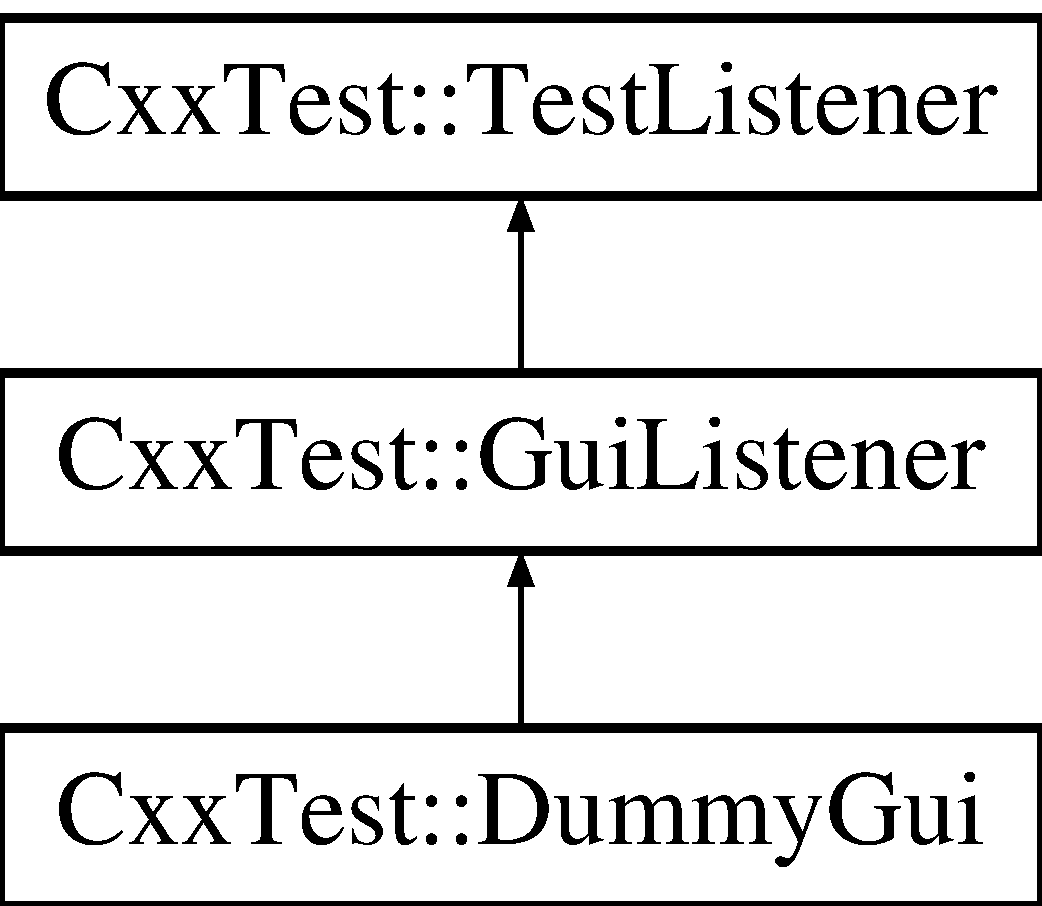
\includegraphics[height=3.000000cm]{classCxxTest_1_1DummyGui}
\end{center}
\end{figure}
\subsection*{Public Member Functions}
\begin{DoxyCompactItemize}
\item 
\hypertarget{classCxxTest_1_1DummyGui_a15b0222f2faf7b291164fd2520c02a87}{void {\bfseries gui\-Enter\-World} (unsigned num\-Total\-Tests)}\label{classCxxTest_1_1DummyGui_a15b0222f2faf7b291164fd2520c02a87}

\item 
\hypertarget{classCxxTest_1_1DummyGui_af62bf6f68c3f8d7d14c02e0ab479b0d1}{void {\bfseries gui\-Enter\-Test} (const char $\ast$suite\-Name, const char $\ast$test\-Name)}\label{classCxxTest_1_1DummyGui_af62bf6f68c3f8d7d14c02e0ab479b0d1}

\item 
\hypertarget{classCxxTest_1_1DummyGui_aeae4ca8fafa4adb65059a89bb325a6a5}{void {\bfseries yellow\-Bar} ()}\label{classCxxTest_1_1DummyGui_aeae4ca8fafa4adb65059a89bb325a6a5}

\item 
\hypertarget{classCxxTest_1_1DummyGui_ac07820db73af309742c128c9d40d75ab}{void {\bfseries red\-Bar} ()}\label{classCxxTest_1_1DummyGui_ac07820db73af309742c128c9d40d75ab}

\item 
\hypertarget{classCxxTest_1_1DummyGui_ad91d806815c7e4ee195c7003ee552464}{void {\bfseries leave\-World} (const \hyperlink{classCxxTest_1_1WorldDescription}{World\-Description} \&)}\label{classCxxTest_1_1DummyGui_ad91d806815c7e4ee195c7003ee552464}

\end{DoxyCompactItemize}
\subsection*{Additional Inherited Members}


The documentation for this class was generated from the following file\-:\begin{DoxyCompactItemize}
\item 
test/cxxtest/test/cxxtest/Dummy\-Gui.\-h\end{DoxyCompactItemize}

\hypertarget{classCxxTest_1_1DummySuiteDescription}{\section{Cxx\-Test\-:\-:Dummy\-Suite\-Description Class Reference}
\label{classCxxTest_1_1DummySuiteDescription}\index{Cxx\-Test\-::\-Dummy\-Suite\-Description@{Cxx\-Test\-::\-Dummy\-Suite\-Description}}
}
Inheritance diagram for Cxx\-Test\-:\-:Dummy\-Suite\-Description\-:\begin{figure}[H]
\begin{center}
\leavevmode
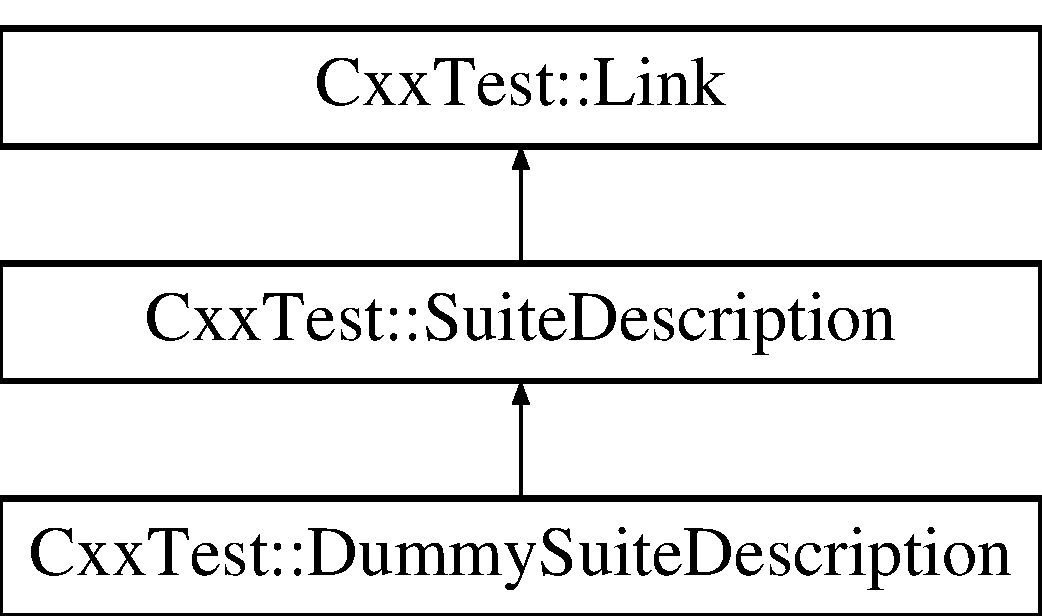
\includegraphics[height=3.000000cm]{classCxxTest_1_1DummySuiteDescription}
\end{center}
\end{figure}
\subsection*{Public Member Functions}
\begin{DoxyCompactItemize}
\item 
\hypertarget{classCxxTest_1_1DummySuiteDescription_a7b28edf5e71e16115eecb5dfe47634d3}{const char $\ast$ {\bfseries file} () const }\label{classCxxTest_1_1DummySuiteDescription_a7b28edf5e71e16115eecb5dfe47634d3}

\item 
\hypertarget{classCxxTest_1_1DummySuiteDescription_a52a1153215623e8ab8a74a6065e18c24}{int {\bfseries line} () const }\label{classCxxTest_1_1DummySuiteDescription_a52a1153215623e8ab8a74a6065e18c24}

\item 
\hypertarget{classCxxTest_1_1DummySuiteDescription_a127442ba0751eac44d7a58d111b6b85e}{const char $\ast$ {\bfseries suite\-Name} () const }\label{classCxxTest_1_1DummySuiteDescription_a127442ba0751eac44d7a58d111b6b85e}

\item 
\hypertarget{classCxxTest_1_1DummySuiteDescription_a468a690741c697e004293a7743835e92}{\hyperlink{classCxxTest_1_1TestSuite}{Test\-Suite} $\ast$ {\bfseries suite} () const }\label{classCxxTest_1_1DummySuiteDescription_a468a690741c697e004293a7743835e92}

\item 
\hypertarget{classCxxTest_1_1DummySuiteDescription_a842b33fdb7947ccec0b970900a6e29a0}{unsigned {\bfseries num\-Tests} () const }\label{classCxxTest_1_1DummySuiteDescription_a842b33fdb7947ccec0b970900a6e29a0}

\item 
\hypertarget{classCxxTest_1_1DummySuiteDescription_a316d81f0134d18b50be4d4d84d798895}{const \hyperlink{classCxxTest_1_1TestDescription}{Test\-Description} \& {\bfseries test\-Description} (unsigned) const }\label{classCxxTest_1_1DummySuiteDescription_a316d81f0134d18b50be4d4d84d798895}

\item 
\hypertarget{classCxxTest_1_1DummySuiteDescription_a4215f951042621608a176b65384dd540}{\hyperlink{classCxxTest_1_1SuiteDescription}{Suite\-Description} $\ast$ {\bfseries next} ()}\label{classCxxTest_1_1DummySuiteDescription_a4215f951042621608a176b65384dd540}

\item 
\hypertarget{classCxxTest_1_1DummySuiteDescription_a0915da66e14e88a117b559cd30d5e3cb}{\hyperlink{classCxxTest_1_1TestDescription}{Test\-Description} $\ast$ {\bfseries first\-Test} ()}\label{classCxxTest_1_1DummySuiteDescription_a0915da66e14e88a117b559cd30d5e3cb}

\item 
\hypertarget{classCxxTest_1_1DummySuiteDescription_a375e255366523dae2bf42b30644ab924}{const \hyperlink{classCxxTest_1_1SuiteDescription}{Suite\-Description} $\ast$ {\bfseries next} () const }\label{classCxxTest_1_1DummySuiteDescription_a375e255366523dae2bf42b30644ab924}

\item 
\hypertarget{classCxxTest_1_1DummySuiteDescription_a3f14f70a29bde28dfede9627f684baa5}{const \hyperlink{classCxxTest_1_1TestDescription}{Test\-Description} $\ast$ {\bfseries first\-Test} () const }\label{classCxxTest_1_1DummySuiteDescription_a3f14f70a29bde28dfede9627f684baa5}

\item 
\hypertarget{classCxxTest_1_1DummySuiteDescription_ad0b362a31490c87bcc78d4f00b4026b4}{void {\bfseries activate\-All\-Tests} ()}\label{classCxxTest_1_1DummySuiteDescription_ad0b362a31490c87bcc78d4f00b4026b4}

\item 
\hypertarget{classCxxTest_1_1DummySuiteDescription_a7cf85000912335e4a70aed43190c2845}{bool {\bfseries leave\-Only} (const char $\ast$)}\label{classCxxTest_1_1DummySuiteDescription_a7cf85000912335e4a70aed43190c2845}

\item 
\hypertarget{classCxxTest_1_1DummySuiteDescription_a7c6d90effe118805dd651a8be2ca4582}{bool {\bfseries set\-Up} ()}\label{classCxxTest_1_1DummySuiteDescription_a7c6d90effe118805dd651a8be2ca4582}

\item 
\hypertarget{classCxxTest_1_1DummySuiteDescription_add53762c3405f0b5d159e61f5092ef00}{bool {\bfseries tear\-Down} ()}\label{classCxxTest_1_1DummySuiteDescription_add53762c3405f0b5d159e61f5092ef00}

\end{DoxyCompactItemize}


The documentation for this class was generated from the following files\-:\begin{DoxyCompactItemize}
\item 
test/cxxtest/cxxtest/Dummy\-Descriptions.\-h\item 
test/cxxtest/cxxtest/Dummy\-Descriptions.\-cpp\end{DoxyCompactItemize}

\hypertarget{classCxxTest_1_1DummyTestDescription}{\section{Cxx\-Test\-:\-:Dummy\-Test\-Description Class Reference}
\label{classCxxTest_1_1DummyTestDescription}\index{Cxx\-Test\-::\-Dummy\-Test\-Description@{Cxx\-Test\-::\-Dummy\-Test\-Description}}
}
Inheritance diagram for Cxx\-Test\-:\-:Dummy\-Test\-Description\-:\begin{figure}[H]
\begin{center}
\leavevmode
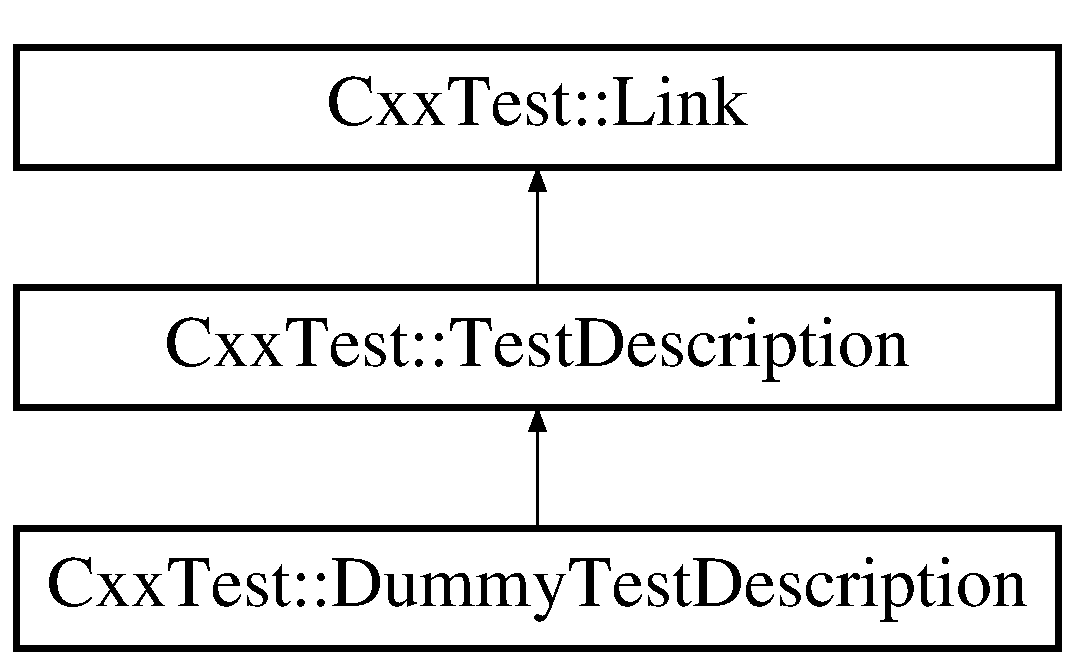
\includegraphics[height=3.000000cm]{classCxxTest_1_1DummyTestDescription}
\end{center}
\end{figure}
\subsection*{Public Member Functions}
\begin{DoxyCompactItemize}
\item 
\hypertarget{classCxxTest_1_1DummyTestDescription_a21005169bb72663e407b45eb27dff403}{const char $\ast$ {\bfseries file} () const }\label{classCxxTest_1_1DummyTestDescription_a21005169bb72663e407b45eb27dff403}

\item 
\hypertarget{classCxxTest_1_1DummyTestDescription_a154f960c20e234070ae79d033d49a0fa}{int {\bfseries line} () const }\label{classCxxTest_1_1DummyTestDescription_a154f960c20e234070ae79d033d49a0fa}

\item 
\hypertarget{classCxxTest_1_1DummyTestDescription_a1798b906914210b3a5c39b1980446703}{const char $\ast$ {\bfseries test\-Name} () const }\label{classCxxTest_1_1DummyTestDescription_a1798b906914210b3a5c39b1980446703}

\item 
\hypertarget{classCxxTest_1_1DummyTestDescription_a672c8c42e2ca9457f376ae5d4c3403b0}{const char $\ast$ {\bfseries suite\-Name} () const }\label{classCxxTest_1_1DummyTestDescription_a672c8c42e2ca9457f376ae5d4c3403b0}

\item 
\hypertarget{classCxxTest_1_1DummyTestDescription_a24f9066548e0d6376ff91467af2aff3a}{bool {\bfseries set\-Up} ()}\label{classCxxTest_1_1DummyTestDescription_a24f9066548e0d6376ff91467af2aff3a}

\item 
\hypertarget{classCxxTest_1_1DummyTestDescription_a8a15205feb0a0f433fd7207e7039cb7a}{void {\bfseries run} ()}\label{classCxxTest_1_1DummyTestDescription_a8a15205feb0a0f433fd7207e7039cb7a}

\item 
\hypertarget{classCxxTest_1_1DummyTestDescription_a89914791c85021c2612a29fbe57a7f99}{bool {\bfseries tear\-Down} ()}\label{classCxxTest_1_1DummyTestDescription_a89914791c85021c2612a29fbe57a7f99}

\item 
\hypertarget{classCxxTest_1_1DummyTestDescription_ac4318fa14c5daff130c272db0331c15f}{\hyperlink{classCxxTest_1_1TestDescription}{Test\-Description} $\ast$ {\bfseries next} ()}\label{classCxxTest_1_1DummyTestDescription_ac4318fa14c5daff130c272db0331c15f}

\item 
\hypertarget{classCxxTest_1_1DummyTestDescription_a5bbce0a879115d14cecec9ef2cbb8dc1}{const \hyperlink{classCxxTest_1_1TestDescription}{Test\-Description} $\ast$ {\bfseries next} () const }\label{classCxxTest_1_1DummyTestDescription_a5bbce0a879115d14cecec9ef2cbb8dc1}

\end{DoxyCompactItemize}


The documentation for this class was generated from the following files\-:\begin{DoxyCompactItemize}
\item 
test/cxxtest/cxxtest/Dummy\-Descriptions.\-h\item 
test/cxxtest/cxxtest/Dummy\-Descriptions.\-cpp\end{DoxyCompactItemize}

\hypertarget{classCxxTest_1_1DummyWorldDescription}{\section{Cxx\-Test\-:\-:Dummy\-World\-Description Class Reference}
\label{classCxxTest_1_1DummyWorldDescription}\index{Cxx\-Test\-::\-Dummy\-World\-Description@{Cxx\-Test\-::\-Dummy\-World\-Description}}
}
Inheritance diagram for Cxx\-Test\-:\-:Dummy\-World\-Description\-:\begin{figure}[H]
\begin{center}
\leavevmode
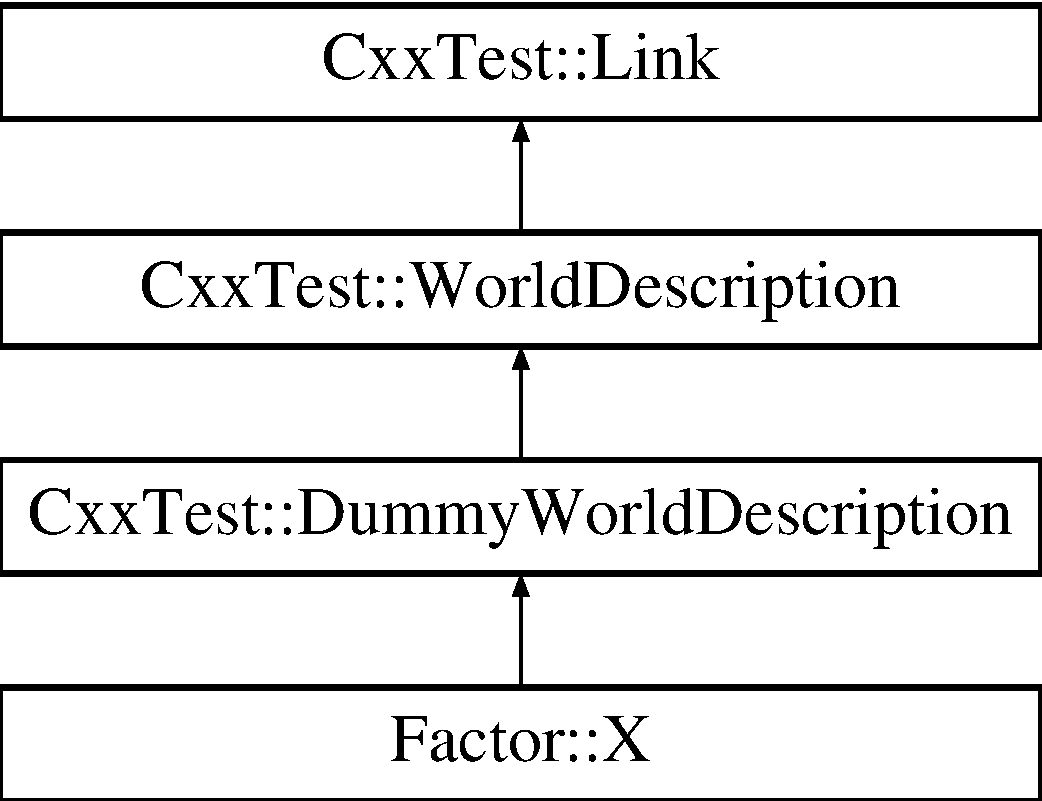
\includegraphics[height=4.000000cm]{classCxxTest_1_1DummyWorldDescription}
\end{center}
\end{figure}
\subsection*{Public Member Functions}
\begin{DoxyCompactItemize}
\item 
\hypertarget{classCxxTest_1_1DummyWorldDescription_a67c8732d9f7af8fba6bfa6af8a50b9b1}{unsigned {\bfseries num\-Suites} (void) const }\label{classCxxTest_1_1DummyWorldDescription_a67c8732d9f7af8fba6bfa6af8a50b9b1}

\item 
\hypertarget{classCxxTest_1_1DummyWorldDescription_a8c22ad8a1322910c12efde300af6ff10}{unsigned {\bfseries num\-Total\-Tests} (void) const }\label{classCxxTest_1_1DummyWorldDescription_a8c22ad8a1322910c12efde300af6ff10}

\item 
\hypertarget{classCxxTest_1_1DummyWorldDescription_a6ac8a1dc038fc842a6393200ed9788de}{const \hyperlink{classCxxTest_1_1SuiteDescription}{Suite\-Description} \& {\bfseries suite\-Description} (unsigned) const }\label{classCxxTest_1_1DummyWorldDescription_a6ac8a1dc038fc842a6393200ed9788de}

\item 
\hypertarget{classCxxTest_1_1DummyWorldDescription_a5898cb8664cf9cdc8ad488d8f7c4faa0}{\hyperlink{classCxxTest_1_1SuiteDescription}{Suite\-Description} $\ast$ {\bfseries first\-Suite} ()}\label{classCxxTest_1_1DummyWorldDescription_a5898cb8664cf9cdc8ad488d8f7c4faa0}

\item 
\hypertarget{classCxxTest_1_1DummyWorldDescription_a0c36115f9bbe671e3b4bc381a6b96671}{const \hyperlink{classCxxTest_1_1SuiteDescription}{Suite\-Description} $\ast$ {\bfseries first\-Suite} () const }\label{classCxxTest_1_1DummyWorldDescription_a0c36115f9bbe671e3b4bc381a6b96671}

\item 
\hypertarget{classCxxTest_1_1DummyWorldDescription_ac0c6f072e9d1d1027c6a6ed3226f4419}{void {\bfseries activate\-All\-Tests} ()}\label{classCxxTest_1_1DummyWorldDescription_ac0c6f072e9d1d1027c6a6ed3226f4419}

\item 
\hypertarget{classCxxTest_1_1DummyWorldDescription_ae063a241c98995268b3df7be8362ff52}{bool {\bfseries leave\-Only} (const char $\ast$, const char $\ast$=0)}\label{classCxxTest_1_1DummyWorldDescription_ae063a241c98995268b3df7be8362ff52}

\item 
\hypertarget{classCxxTest_1_1DummyWorldDescription_a17bf1593f3627dded7f69d71c8172172}{bool {\bfseries set\-Up} ()}\label{classCxxTest_1_1DummyWorldDescription_a17bf1593f3627dded7f69d71c8172172}

\item 
\hypertarget{classCxxTest_1_1DummyWorldDescription_aeac2bd6926e9ce72df8f04bb8c432d5c}{bool {\bfseries tear\-Down} ()}\label{classCxxTest_1_1DummyWorldDescription_aeac2bd6926e9ce72df8f04bb8c432d5c}

\end{DoxyCompactItemize}
\subsection*{Additional Inherited Members}


The documentation for this class was generated from the following files\-:\begin{DoxyCompactItemize}
\item 
test/cxxtest/cxxtest/Dummy\-Descriptions.\-h\item 
test/cxxtest/cxxtest/Dummy\-Descriptions.\-cpp\end{DoxyCompactItemize}

\hypertarget{classDynamicAbort}{\section{Dynamic\-Abort Class Reference}
\label{classDynamicAbort}\index{Dynamic\-Abort@{Dynamic\-Abort}}
}
Inheritance diagram for Dynamic\-Abort\-:\begin{figure}[H]
\begin{center}
\leavevmode
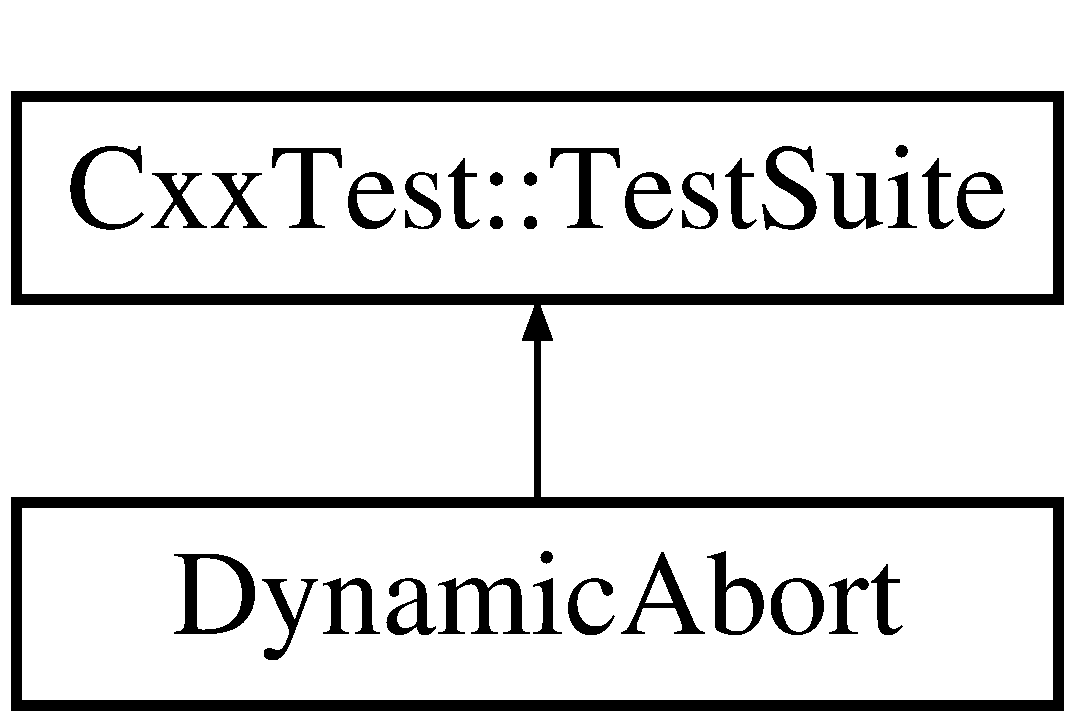
\includegraphics[height=2.000000cm]{classDynamicAbort}
\end{center}
\end{figure}
\subsection*{Public Member Functions}
\begin{DoxyCompactItemize}
\item 
\hypertarget{classDynamicAbort_a2d9c1b9c3a7fd18603efca59a6d98922}{void {\bfseries test\-\_\-\-Abort\-\_\-on\-\_\-fail\-\_\-in\-\_\-this\-\_\-test} ()}\label{classDynamicAbort_a2d9c1b9c3a7fd18603efca59a6d98922}

\item 
\hypertarget{classDynamicAbort_ae3f6ec30e72c5c9f3b286569e4bd381c}{void {\bfseries test\-\_\-\-Dont\-\_\-abort\-\_\-in\-\_\-this\-\_\-test} ()}\label{classDynamicAbort_ae3f6ec30e72c5c9f3b286569e4bd381c}

\item 
\hypertarget{classDynamicAbort_a5db3b66a210c82e7151bb7d3645c93fb}{void {\bfseries test\-\_\-\-Revert\-\_\-to\-\_\-abort} ()}\label{classDynamicAbort_a5db3b66a210c82e7151bb7d3645c93fb}

\end{DoxyCompactItemize}


The documentation for this class was generated from the following file\-:\begin{DoxyCompactItemize}
\item 
test/cxxtest/test/Dynamic\-Abort.\-h\end{DoxyCompactItemize}

\hypertarget{classDynamicMax}{\section{Dynamic\-Max Class Reference}
\label{classDynamicMax}\index{Dynamic\-Max@{Dynamic\-Max}}
}
Inheritance diagram for Dynamic\-Max\-:\begin{figure}[H]
\begin{center}
\leavevmode
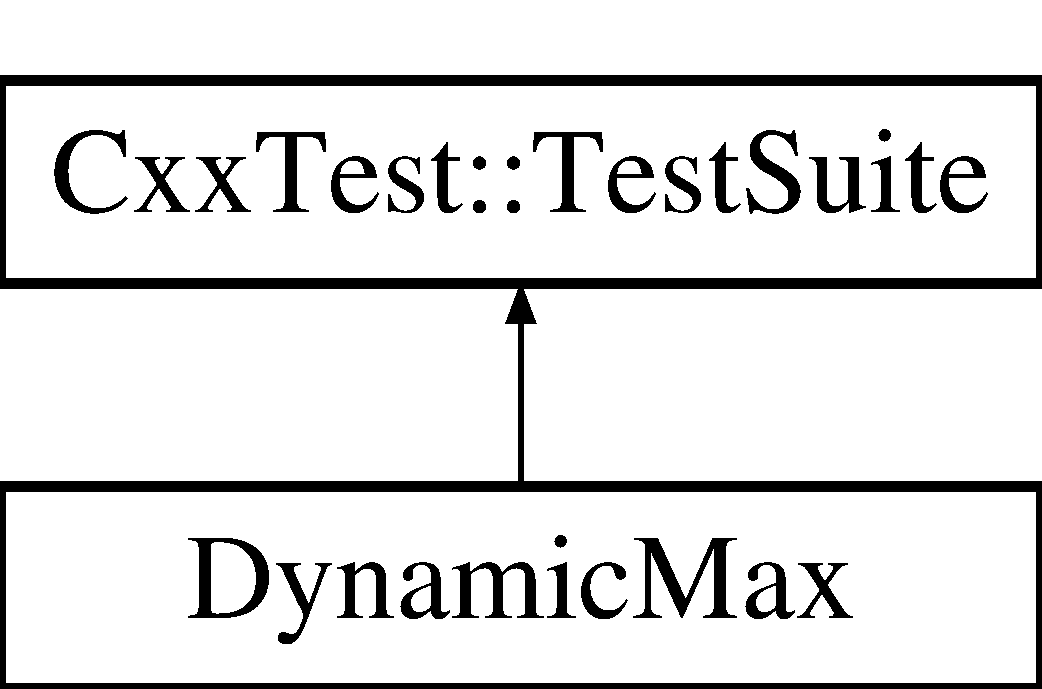
\includegraphics[height=2.000000cm]{classDynamicMax}
\end{center}
\end{figure}
\subsection*{Public Types}
\begin{DoxyCompactItemize}
\item 
enum \{ {\bfseries D\-A\-T\-A\-\_\-\-S\-I\-Z\-E} = 24
 \}
\end{DoxyCompactItemize}
\subsection*{Public Member Functions}
\begin{DoxyCompactItemize}
\item 
\hypertarget{classDynamicMax_a6ef2b80d5b2b70e9d32c41361ff5a30c}{void {\bfseries set\-Up} ()}\label{classDynamicMax_a6ef2b80d5b2b70e9d32c41361ff5a30c}

\item 
\hypertarget{classDynamicMax_af78ea919f278a663aef09a9adf93f010}{void {\bfseries test\-\_\-\-Max\-\_\-size\-\_\-from\-\_\-define} ()}\label{classDynamicMax_af78ea919f278a663aef09a9adf93f010}

\item 
\hypertarget{classDynamicMax_aab7c9b0ecc72d795e4935eaa53e83b6f}{void {\bfseries test\-\_\-\-Set\-\_\-max\-\_\-size} ()}\label{classDynamicMax_aab7c9b0ecc72d795e4935eaa53e83b6f}

\item 
\hypertarget{classDynamicMax_a851765fa33488833e3fd4ba5a386f3f4}{void {\bfseries test\-\_\-\-Revert\-\_\-to\-\_\-max\-\_\-size\-\_\-from\-\_\-define} ()}\label{classDynamicMax_a851765fa33488833e3fd4ba5a386f3f4}

\item 
\hypertarget{classDynamicMax_af50d3b8128f9f901fcecfbf8a6d9e36e}{void {\bfseries test\-\_\-\-Set\-\_\-max\-\_\-size\-\_\-to\-\_\-zero\-\_\-\-\_\-dumps\-\_\-all} ()}\label{classDynamicMax_af50d3b8128f9f901fcecfbf8a6d9e36e}

\end{DoxyCompactItemize}
\subsection*{Public Attributes}
\begin{DoxyCompactItemize}
\item 
\hypertarget{classDynamicMax_a1eb90dc5efcd810759bb613d3acb2290}{unsigned char {\bfseries x} \mbox{[}D\-A\-T\-A\-\_\-\-S\-I\-Z\-E\mbox{]}}\label{classDynamicMax_a1eb90dc5efcd810759bb613d3acb2290}

\item 
\hypertarget{classDynamicMax_a7786547534a3a5c66c523ccb73425c7a}{unsigned char {\bfseries y} \mbox{[}D\-A\-T\-A\-\_\-\-S\-I\-Z\-E\mbox{]}}\label{classDynamicMax_a7786547534a3a5c66c523ccb73425c7a}

\end{DoxyCompactItemize}


The documentation for this class was generated from the following file\-:\begin{DoxyCompactItemize}
\item 
test/cxxtest/test/Dynamic\-Max.\-h\end{DoxyCompactItemize}

\hypertarget{classCxxTest_1_1DynamicSuiteDescription}{\section{Cxx\-Test\-:\-:Dynamic\-Suite\-Description$<$ S $>$ Class Template Reference}
\label{classCxxTest_1_1DynamicSuiteDescription}\index{Cxx\-Test\-::\-Dynamic\-Suite\-Description$<$ S $>$@{Cxx\-Test\-::\-Dynamic\-Suite\-Description$<$ S $>$}}
}
Inheritance diagram for Cxx\-Test\-:\-:Dynamic\-Suite\-Description$<$ S $>$\-:\begin{figure}[H]
\begin{center}
\leavevmode
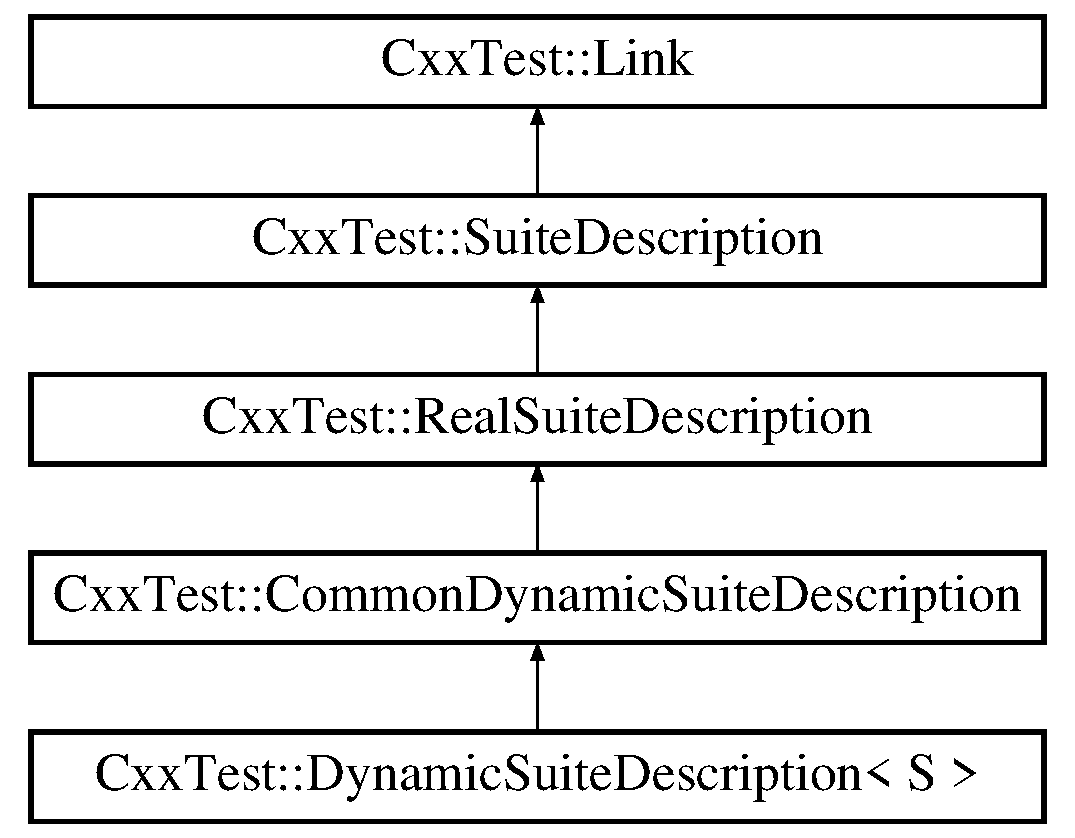
\includegraphics[height=5.000000cm]{classCxxTest_1_1DynamicSuiteDescription}
\end{center}
\end{figure}
\subsection*{Public Member Functions}
\begin{DoxyCompactItemize}
\item 
\hypertarget{classCxxTest_1_1DynamicSuiteDescription_ab325f0a2e81ebbb6719f780d75471883}{{\bfseries Dynamic\-Suite\-Description} (const char $\ast$arg\-File, unsigned arg\-Line, const char $\ast$arg\-Suite\-Name, \hyperlink{structCxxTest_1_1List}{List} \&arg\-Tests, S $\ast$\&arg\-Suite, unsigned arg\-Create\-Line, unsigned arg\-Destroy\-Line)}\label{classCxxTest_1_1DynamicSuiteDescription_ab325f0a2e81ebbb6719f780d75471883}

\item 
\hypertarget{classCxxTest_1_1DynamicSuiteDescription_a0f426c051f5ccaf14ebbd11c07329e57}{void {\bfseries initialize} (const char $\ast$arg\-File, unsigned arg\-Line, const char $\ast$arg\-Suite\-Name, \hyperlink{structCxxTest_1_1List}{List} \&arg\-Tests, S $\ast$\&arg\-Suite, unsigned arg\-Create\-Line, unsigned arg\-Destroy\-Line)}\label{classCxxTest_1_1DynamicSuiteDescription_a0f426c051f5ccaf14ebbd11c07329e57}

\item 
\hypertarget{classCxxTest_1_1DynamicSuiteDescription_a524a9a8981a9c58aa09023d3bfba4dee}{\hyperlink{classCxxTest_1_1TestSuite}{Test\-Suite} $\ast$ {\bfseries suite} () const }\label{classCxxTest_1_1DynamicSuiteDescription_a524a9a8981a9c58aa09023d3bfba4dee}

\item 
\hypertarget{classCxxTest_1_1DynamicSuiteDescription_a0cee600a803f0accaaa82a1e933d2266}{bool {\bfseries set\-Up} ()}\label{classCxxTest_1_1DynamicSuiteDescription_a0cee600a803f0accaaa82a1e933d2266}

\item 
\hypertarget{classCxxTest_1_1DynamicSuiteDescription_a322a0b084882a891bc8cf12805a56f12}{bool {\bfseries tear\-Down} ()}\label{classCxxTest_1_1DynamicSuiteDescription_a322a0b084882a891bc8cf12805a56f12}

\end{DoxyCompactItemize}
\subsection*{Additional Inherited Members}


The documentation for this class was generated from the following file\-:\begin{DoxyCompactItemize}
\item 
test/cxxtest/cxxtest/Real\-Descriptions.\-h\end{DoxyCompactItemize}

\hypertarget{structDefaultTraits_1_1EightBytes}{\section{Default\-Traits\-:\-:Eight\-Bytes Struct Reference}
\label{structDefaultTraits_1_1EightBytes}\index{Default\-Traits\-::\-Eight\-Bytes@{Default\-Traits\-::\-Eight\-Bytes}}
}
\subsection*{Public Attributes}
\begin{DoxyCompactItemize}
\item 
\hypertarget{structDefaultTraits_1_1EightBytes_a5abb3681c7116c3854e750564a984d4c}{unsigned char {\bfseries data} \mbox{[}8\mbox{]}}\label{structDefaultTraits_1_1EightBytes_a5abb3681c7116c3854e750564a984d4c}

\end{DoxyCompactItemize}


The documentation for this struct was generated from the following file\-:\begin{DoxyCompactItemize}
\item 
test/cxxtest/test/Default\-Traits.\-h\end{DoxyCompactItemize}

\hypertarget{classCxxTest_1_1ElementInfo}{\section{Cxx\-Test\-:\-:Element\-Info Class Reference}
\label{classCxxTest_1_1ElementInfo}\index{Cxx\-Test\-::\-Element\-Info@{Cxx\-Test\-::\-Element\-Info}}
}
\subsection*{Public Member Functions}
\begin{DoxyCompactItemize}
\item 
\hypertarget{classCxxTest_1_1ElementInfo_af577f64e81c279a003898ba3d8ceffcb}{{\bfseries Element\-Info} (const \hyperlink{classCxxTest_1_1ElementInfo}{Element\-Info} \&rhs)}\label{classCxxTest_1_1ElementInfo_af577f64e81c279a003898ba3d8ceffcb}

\item 
\hypertarget{classCxxTest_1_1ElementInfo_a53b08224991e1c0cf2f0321186cfc0cc}{\hyperlink{classCxxTest_1_1ElementInfo}{Element\-Info} \& {\bfseries operator=} (const \hyperlink{classCxxTest_1_1ElementInfo}{Element\-Info} \&rhs)}\label{classCxxTest_1_1ElementInfo_a53b08224991e1c0cf2f0321186cfc0cc}

\item 
\hypertarget{classCxxTest_1_1ElementInfo_ab23be1c4afc1250d01efa9a277c63411}{{\footnotesize template$<$class Type $>$ }\\void {\bfseries add} (const std\-::string \&name\-\_\-, Type \&value\-\_\-)}\label{classCxxTest_1_1ElementInfo_ab23be1c4afc1250d01efa9a277c63411}

\item 
\hypertarget{classCxxTest_1_1ElementInfo_a55047cf35e4208b8b58e7570de75c81b}{void {\bfseries write} (\hyperlink{classCxxTest_1_1OutputStream}{Output\-Stream} \&os)}\label{classCxxTest_1_1ElementInfo_a55047cf35e4208b8b58e7570de75c81b}

\item 
\hypertarget{classCxxTest_1_1ElementInfo_ae8d1b9bfff2bdc2feee7f6a8b1d5bba9}{std\-::string {\bfseries escape} (const std\-::string \&str)}\label{classCxxTest_1_1ElementInfo_ae8d1b9bfff2bdc2feee7f6a8b1d5bba9}

\end{DoxyCompactItemize}
\subsection*{Public Attributes}
\begin{DoxyCompactItemize}
\item 
\hypertarget{classCxxTest_1_1ElementInfo_a168065b70d5784d05560ce2fb7163356}{std\-::string {\bfseries name}}\label{classCxxTest_1_1ElementInfo_a168065b70d5784d05560ce2fb7163356}

\item 
\hypertarget{classCxxTest_1_1ElementInfo_a080e05f851a2f0a6c56f3b8e9c77b8e2}{std\-::stringstream {\bfseries value}}\label{classCxxTest_1_1ElementInfo_a080e05f851a2f0a6c56f3b8e9c77b8e2}

\item 
\hypertarget{classCxxTest_1_1ElementInfo_a4e81871282b9dbe53a6b6493c6d53c6f}{std\-::map$<$ std\-::string, \\*
std\-::string $>$ {\bfseries attribute}}\label{classCxxTest_1_1ElementInfo_a4e81871282b9dbe53a6b6493c6d53c6f}

\end{DoxyCompactItemize}


The documentation for this class was generated from the following file\-:\begin{DoxyCompactItemize}
\item 
test/cxxtest/cxxtest/Xml\-Formatter.\-h\end{DoxyCompactItemize}

\hypertarget{classEmptySuite}{\section{Empty\-Suite Class Reference}
\label{classEmptySuite}\index{Empty\-Suite@{Empty\-Suite}}
}
Inheritance diagram for Empty\-Suite\-:\begin{figure}[H]
\begin{center}
\leavevmode
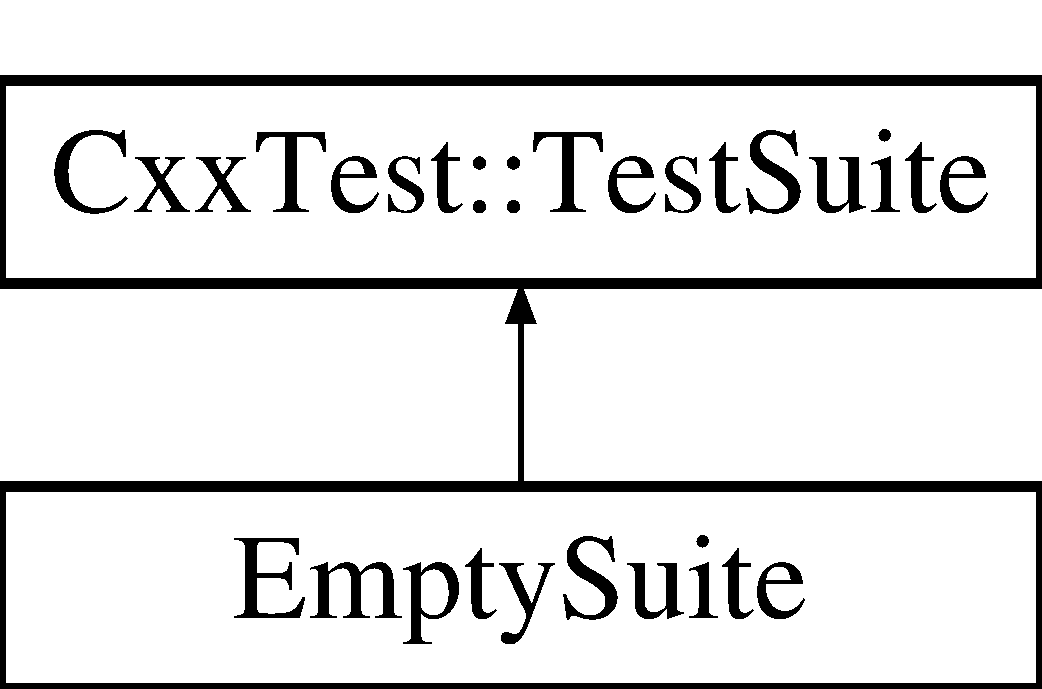
\includegraphics[height=2.000000cm]{classEmptySuite}
\end{center}
\end{figure}
\subsection*{Public Member Functions}
\begin{DoxyCompactItemize}
\item 
\hypertarget{classEmptySuite_a3f211d708f6a9aa583a7c888874a44f8}{void {\bfseries set\-Up} ()}\label{classEmptySuite_a3f211d708f6a9aa583a7c888874a44f8}

\item 
\hypertarget{classEmptySuite_adfea273a276b498d0f572b620d47d369}{void {\bfseries tear\-Down} ()}\label{classEmptySuite_adfea273a276b498d0f572b620d47d369}

\item 
\hypertarget{classEmptySuite_a731ab1740e5b588793b63a312aaad00d}{void {\bfseries this\-Suite\-Has\-No\-Tests} ()}\label{classEmptySuite_a731ab1740e5b588793b63a312aaad00d}

\end{DoxyCompactItemize}
\subsection*{Static Public Member Functions}
\begin{DoxyCompactItemize}
\item 
\hypertarget{classEmptySuite_a7cf7f1b3e84258059351be4f225a1d00}{static \hyperlink{classEmptySuite}{Empty\-Suite} $\ast$ {\bfseries create\-Suite} ()}\label{classEmptySuite_a7cf7f1b3e84258059351be4f225a1d00}

\item 
\hypertarget{classEmptySuite_a89687ffb4751bfb77dbca9eb89c3c5af}{static void {\bfseries destroy\-Suite} (\hyperlink{classEmptySuite}{Empty\-Suite} $\ast$suite)}\label{classEmptySuite_a89687ffb4751bfb77dbca9eb89c3c5af}

\end{DoxyCompactItemize}


The documentation for this class was generated from the following file\-:\begin{DoxyCompactItemize}
\item 
test/cxxtest/test/Empty\-Suite.\-h\end{DoxyCompactItemize}

\hypertarget{classEnumTraits}{\section{Enum\-Traits Class Reference}
\label{classEnumTraits}\index{Enum\-Traits@{Enum\-Traits}}
}
Inheritance diagram for Enum\-Traits\-:\begin{figure}[H]
\begin{center}
\leavevmode
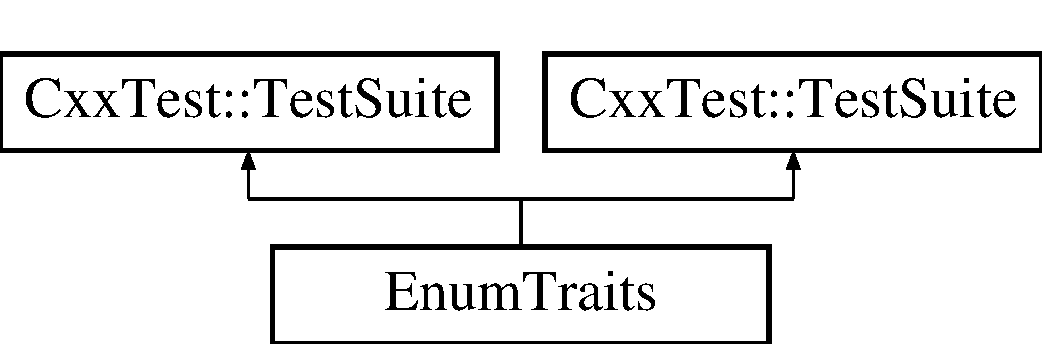
\includegraphics[height=2.000000cm]{classEnumTraits}
\end{center}
\end{figure}
\subsection*{Public Member Functions}
\begin{DoxyCompactItemize}
\item 
\hypertarget{classEnumTraits_a047802487e9741e9a8b4a7cf5e93e3b6}{void {\bfseries test\-\_\-\-Enum\-\_\-traits} ()}\label{classEnumTraits_a047802487e9741e9a8b4a7cf5e93e3b6}

\item 
\hypertarget{classEnumTraits_a047802487e9741e9a8b4a7cf5e93e3b6}{void {\bfseries test\-\_\-\-Enum\-\_\-traits} ()}\label{classEnumTraits_a047802487e9741e9a8b4a7cf5e93e3b6}

\end{DoxyCompactItemize}


The documentation for this class was generated from the following files\-:\begin{DoxyCompactItemize}
\item 
test/cxxtest/doc/examples/My\-Test\-Suite9.\-h\item 
test/cxxtest/sample/Enum\-Traits.\-h\end{DoxyCompactItemize}

\hypertarget{structCxxTest_1_1equals}{\section{Cxx\-Test\-:\-:equals$<$ X, Y $>$ Struct Template Reference}
\label{structCxxTest_1_1equals}\index{Cxx\-Test\-::equals$<$ X, Y $>$@{Cxx\-Test\-::equals$<$ X, Y $>$}}
}
\subsection*{Static Public Member Functions}
\begin{DoxyCompactItemize}
\item 
\hypertarget{structCxxTest_1_1equals_a03a782c1be1468c9ea2bc16ae8a39e27}{static bool {\bfseries test} (\hyperlink{classX}{X} x, Y y)}\label{structCxxTest_1_1equals_a03a782c1be1468c9ea2bc16ae8a39e27}

\end{DoxyCompactItemize}


The documentation for this struct was generated from the following file\-:\begin{DoxyCompactItemize}
\item 
test/cxxtest/cxxtest/Test\-Suite.\-h\end{DoxyCompactItemize}

\hypertarget{structCxxTest_1_1equals_3_01char_01_5_00_01char_01_5_01_4}{\section{Cxx\-Test\-:\-:equals$<$ char $\ast$, char $\ast$ $>$ Struct Template Reference}
\label{structCxxTest_1_1equals_3_01char_01_5_00_01char_01_5_01_4}\index{Cxx\-Test\-::equals$<$ char $\ast$, char $\ast$ $>$@{Cxx\-Test\-::equals$<$ char $\ast$, char $\ast$ $>$}}
}
\subsection*{Static Public Member Functions}
\begin{DoxyCompactItemize}
\item 
\hypertarget{structCxxTest_1_1equals_3_01char_01_5_00_01char_01_5_01_4_abf9705e6047421967f889dfe5c8320d1}{static bool {\bfseries test} (char $\ast$x, char $\ast$y)}\label{structCxxTest_1_1equals_3_01char_01_5_00_01char_01_5_01_4_abf9705e6047421967f889dfe5c8320d1}

\end{DoxyCompactItemize}


The documentation for this struct was generated from the following file\-:\begin{DoxyCompactItemize}
\item 
test/cxxtest/cxxtest/Test\-Suite.\-h\end{DoxyCompactItemize}

\hypertarget{structCxxTest_1_1equals_3_01char_01_5_00_01const_01char_01_5_01_4}{\section{Cxx\-Test\-:\-:equals$<$ char $\ast$, const char $\ast$ $>$ Struct Template Reference}
\label{structCxxTest_1_1equals_3_01char_01_5_00_01const_01char_01_5_01_4}\index{Cxx\-Test\-::equals$<$ char $\ast$, const char $\ast$ $>$@{Cxx\-Test\-::equals$<$ char $\ast$, const char $\ast$ $>$}}
}
\subsection*{Static Public Member Functions}
\begin{DoxyCompactItemize}
\item 
\hypertarget{structCxxTest_1_1equals_3_01char_01_5_00_01const_01char_01_5_01_4_a8977abbec5e6efaf1882b954fa35dfa1}{static bool {\bfseries test} (char $\ast$x, const char $\ast$y)}\label{structCxxTest_1_1equals_3_01char_01_5_00_01const_01char_01_5_01_4_a8977abbec5e6efaf1882b954fa35dfa1}

\end{DoxyCompactItemize}


The documentation for this struct was generated from the following file\-:\begin{DoxyCompactItemize}
\item 
test/cxxtest/cxxtest/Test\-Suite.\-h\end{DoxyCompactItemize}

\hypertarget{structCxxTest_1_1equals_3_01const_01char_01_5_00_01char_01_5_01_4}{\section{Cxx\-Test\-:\-:equals$<$ const char $\ast$, char $\ast$ $>$ Struct Template Reference}
\label{structCxxTest_1_1equals_3_01const_01char_01_5_00_01char_01_5_01_4}\index{Cxx\-Test\-::equals$<$ const char $\ast$, char $\ast$ $>$@{Cxx\-Test\-::equals$<$ const char $\ast$, char $\ast$ $>$}}
}
\subsection*{Static Public Member Functions}
\begin{DoxyCompactItemize}
\item 
\hypertarget{structCxxTest_1_1equals_3_01const_01char_01_5_00_01char_01_5_01_4_a0ef6cf5c395ca32eb898774f4a1aabe2}{static bool {\bfseries test} (const char $\ast$x, char $\ast$y)}\label{structCxxTest_1_1equals_3_01const_01char_01_5_00_01char_01_5_01_4_a0ef6cf5c395ca32eb898774f4a1aabe2}

\end{DoxyCompactItemize}


The documentation for this struct was generated from the following file\-:\begin{DoxyCompactItemize}
\item 
test/cxxtest/cxxtest/Test\-Suite.\-h\end{DoxyCompactItemize}

\hypertarget{structCxxTest_1_1equals_3_01const_01char_01_5_00_01const_01char_01_5_01_4}{\section{Cxx\-Test\-:\-:equals$<$ const char $\ast$, const char $\ast$ $>$ Struct Template Reference}
\label{structCxxTest_1_1equals_3_01const_01char_01_5_00_01const_01char_01_5_01_4}\index{Cxx\-Test\-::equals$<$ const char $\ast$, const char $\ast$ $>$@{Cxx\-Test\-::equals$<$ const char $\ast$, const char $\ast$ $>$}}
}
\subsection*{Static Public Member Functions}
\begin{DoxyCompactItemize}
\item 
\hypertarget{structCxxTest_1_1equals_3_01const_01char_01_5_00_01const_01char_01_5_01_4_a8a51a5f3c3246e3808548f99c0f134cb}{static bool {\bfseries test} (const char $\ast$x, const char $\ast$y)}\label{structCxxTest_1_1equals_3_01const_01char_01_5_00_01const_01char_01_5_01_4_a8a51a5f3c3246e3808548f99c0f134cb}

\end{DoxyCompactItemize}


The documentation for this struct was generated from the following file\-:\begin{DoxyCompactItemize}
\item 
test/cxxtest/cxxtest/Test\-Suite.\-h\end{DoxyCompactItemize}

\hypertarget{classEraser}{\section{Eraser Class Reference}
\label{classEraser}\index{Eraser@{Eraser}}
}
Inheritance diagram for Eraser\-:\begin{figure}[H]
\begin{center}
\leavevmode
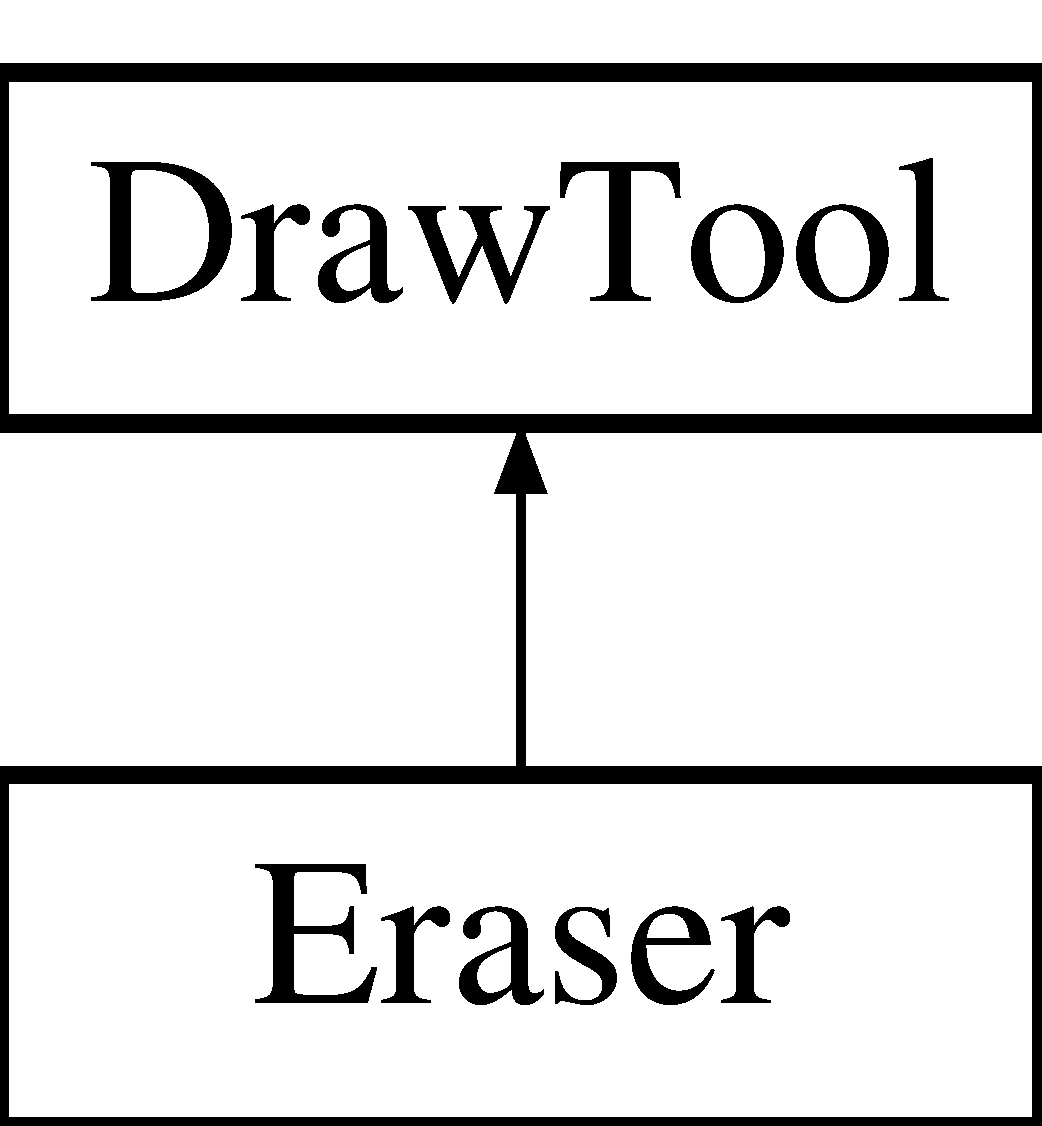
\includegraphics[height=2.000000cm]{classEraser}
\end{center}
\end{figure}
\subsection*{Public Member Functions}
\begin{DoxyCompactItemize}
\item 
\hypertarget{classEraser_a60abccb4522452a4cdfb714eafbc9c16}{{\bfseries Eraser} (int radius)}\label{classEraser_a60abccb4522452a4cdfb714eafbc9c16}

\item 
\hypertarget{classEraser_a195eeec6843317ee33e0e51fccb3daff}{void {\bfseries apply\-Influence} (int x, int y, \hyperlink{classPixelBuffer}{Pixel\-Buffer} $\ast$buffer)}\label{classEraser_a195eeec6843317ee33e0e51fccb3daff}

\item 
\hypertarget{classEraser_ad718ebd5796e0a83dbd94aa4f0ce2921}{void {\bfseries fill\-Influence} ()}\label{classEraser_ad718ebd5796e0a83dbd94aa4f0ce2921}

\item 
\hypertarget{classEraser_a60abccb4522452a4cdfb714eafbc9c16}{{\bfseries Eraser} (int radius)}\label{classEraser_a60abccb4522452a4cdfb714eafbc9c16}

\item 
\hypertarget{classEraser_a195eeec6843317ee33e0e51fccb3daff}{void {\bfseries apply\-Influence} (int x, int y, \hyperlink{classPixelBuffer}{Pixel\-Buffer} $\ast$buffer)}\label{classEraser_a195eeec6843317ee33e0e51fccb3daff}

\item 
\hypertarget{classEraser_ad718ebd5796e0a83dbd94aa4f0ce2921}{void {\bfseries fill\-Influence} ()}\label{classEraser_ad718ebd5796e0a83dbd94aa4f0ce2921}

\item 
\hypertarget{classEraser_a60abccb4522452a4cdfb714eafbc9c16}{{\bfseries Eraser} (int radius)}\label{classEraser_a60abccb4522452a4cdfb714eafbc9c16}

\item 
\hypertarget{classEraser_a195eeec6843317ee33e0e51fccb3daff}{void {\bfseries apply\-Influence} (int x, int y, \hyperlink{classPixelBuffer}{Pixel\-Buffer} $\ast$buffer)}\label{classEraser_a195eeec6843317ee33e0e51fccb3daff}

\item 
\hypertarget{classEraser_ad718ebd5796e0a83dbd94aa4f0ce2921}{void {\bfseries fill\-Influence} ()}\label{classEraser_ad718ebd5796e0a83dbd94aa4f0ce2921}

\end{DoxyCompactItemize}
\subsection*{Additional Inherited Members}


The documentation for this class was generated from the following files\-:\begin{DoxyCompactItemize}
\item 
libphoto/Eraser.\-h\item 
libphoto/include/libphoto.\-h\item 
libphoto/Eraser.\-cpp\end{DoxyCompactItemize}

\hypertarget{classCxxTest_1_1ErrorFormatter}{\section{Cxx\-Test\-:\-:Error\-Formatter Class Reference}
\label{classCxxTest_1_1ErrorFormatter}\index{Cxx\-Test\-::\-Error\-Formatter@{Cxx\-Test\-::\-Error\-Formatter}}
}
Inheritance diagram for Cxx\-Test\-:\-:Error\-Formatter\-:\begin{figure}[H]
\begin{center}
\leavevmode
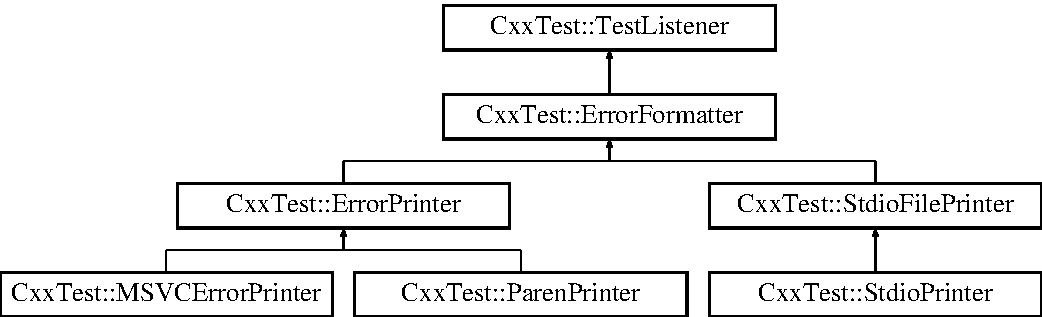
\includegraphics[height=4.000000cm]{classCxxTest_1_1ErrorFormatter}
\end{center}
\end{figure}
\subsection*{Public Member Functions}
\begin{DoxyCompactItemize}
\item 
\hypertarget{classCxxTest_1_1ErrorFormatter_a9a6363f7a4b3aca6cdaeb6111826e7de}{{\bfseries Error\-Formatter} (\hyperlink{classCxxTest_1_1OutputStream}{Output\-Stream} $\ast$o, const char $\ast$pre\-Line=\char`\"{}\-:\char`\"{}, const char $\ast$post\-Line=\char`\"{}\char`\"{}, const char $\ast$error\-String=\char`\"{}Error\char`\"{}, const char $\ast$warning\-String=\char`\"{}Warning\char`\"{})}\label{classCxxTest_1_1ErrorFormatter_a9a6363f7a4b3aca6cdaeb6111826e7de}

\item 
\hypertarget{classCxxTest_1_1ErrorFormatter_a864e271c4a95907866d483a460aa5f71}{int {\bfseries run} ()}\label{classCxxTest_1_1ErrorFormatter_a864e271c4a95907866d483a460aa5f71}

\item 
\hypertarget{classCxxTest_1_1ErrorFormatter_aadd286f416ba8cf6df836863e7a44884}{void {\bfseries enter\-World} (const \hyperlink{classCxxTest_1_1WorldDescription}{World\-Description} \&desc)}\label{classCxxTest_1_1ErrorFormatter_aadd286f416ba8cf6df836863e7a44884}

\item 
\hypertarget{classCxxTest_1_1ErrorFormatter_a72d81800df02cedef86fa3bb7e6a736f}{void {\bfseries enter\-Suite} (const \hyperlink{classCxxTest_1_1SuiteDescription}{Suite\-Description} \&)}\label{classCxxTest_1_1ErrorFormatter_a72d81800df02cedef86fa3bb7e6a736f}

\item 
\hypertarget{classCxxTest_1_1ErrorFormatter_a4cf5c3068bcfe3478a02a16c5ab9dca3}{void {\bfseries enter\-Test} (const \hyperlink{classCxxTest_1_1TestDescription}{Test\-Description} \&)}\label{classCxxTest_1_1ErrorFormatter_a4cf5c3068bcfe3478a02a16c5ab9dca3}

\item 
\hypertarget{classCxxTest_1_1ErrorFormatter_a59d77ff2f2b8ff3715e7fb3938914dc5}{void {\bfseries leave\-Test} (const \hyperlink{classCxxTest_1_1TestDescription}{Test\-Description} \&)}\label{classCxxTest_1_1ErrorFormatter_a59d77ff2f2b8ff3715e7fb3938914dc5}

\item 
\hypertarget{classCxxTest_1_1ErrorFormatter_a68b02ba2222576fcdad50be38672b5c9}{void {\bfseries leave\-World} (const \hyperlink{classCxxTest_1_1WorldDescription}{World\-Description} \&desc)}\label{classCxxTest_1_1ErrorFormatter_a68b02ba2222576fcdad50be38672b5c9}

\item 
\hypertarget{classCxxTest_1_1ErrorFormatter_ad0fd347bdbc3ab84b740efd03a237125}{void {\bfseries trace} (const char $\ast$file, int line, const char $\ast$expression)}\label{classCxxTest_1_1ErrorFormatter_ad0fd347bdbc3ab84b740efd03a237125}

\item 
\hypertarget{classCxxTest_1_1ErrorFormatter_a14de8269504c13f1fa018d7c2a8ba639}{void {\bfseries warning} (const char $\ast$file, int line, const char $\ast$expression)}\label{classCxxTest_1_1ErrorFormatter_a14de8269504c13f1fa018d7c2a8ba639}

\item 
\hypertarget{classCxxTest_1_1ErrorFormatter_a194564b43f7afc8fc0e06cd976813a92}{void {\bfseries skipped\-Test} (const char $\ast$file, int line, const char $\ast$expression)}\label{classCxxTest_1_1ErrorFormatter_a194564b43f7afc8fc0e06cd976813a92}

\item 
\hypertarget{classCxxTest_1_1ErrorFormatter_ae8d8bc67f9d194e8f6357ee0e853ed49}{void {\bfseries failed\-Test} (const char $\ast$file, int line, const char $\ast$expression)}\label{classCxxTest_1_1ErrorFormatter_ae8d8bc67f9d194e8f6357ee0e853ed49}

\item 
\hypertarget{classCxxTest_1_1ErrorFormatter_a745afae529869c8718bab3567e0d2d27}{void {\bfseries failed\-Assert} (const char $\ast$file, int line, const char $\ast$expression)}\label{classCxxTest_1_1ErrorFormatter_a745afae529869c8718bab3567e0d2d27}

\item 
\hypertarget{classCxxTest_1_1ErrorFormatter_aef0fb796b7fb3afc4e625b4f8f489740}{void {\bfseries failed\-Assert\-Equals} (const char $\ast$file, int line, const char $\ast$x\-Str, const char $\ast$y\-Str, const char $\ast$x, const char $\ast$y)}\label{classCxxTest_1_1ErrorFormatter_aef0fb796b7fb3afc4e625b4f8f489740}

\item 
\hypertarget{classCxxTest_1_1ErrorFormatter_ad51758eb24a74031d2b7d42372f8dcb6}{void {\bfseries failed\-Assert\-Same\-Data} (const char $\ast$file, int line, const char $\ast$x\-Str, const char $\ast$y\-Str, const char $\ast$size\-Str, const void $\ast$x, const void $\ast$y, unsigned size)}\label{classCxxTest_1_1ErrorFormatter_ad51758eb24a74031d2b7d42372f8dcb6}

\item 
\hypertarget{classCxxTest_1_1ErrorFormatter_aed7b9a1918cfdd72f966b41ae6023779}{void {\bfseries failed\-Assert\-Same\-Files} (const char $\ast$file, int line, const char $\ast$, const char $\ast$, const char $\ast$explanation)}\label{classCxxTest_1_1ErrorFormatter_aed7b9a1918cfdd72f966b41ae6023779}

\item 
\hypertarget{classCxxTest_1_1ErrorFormatter_ac2c9e5c1f2f2659f06c7e0278a0b09d4}{void {\bfseries failed\-Assert\-Delta} (const char $\ast$file, int line, const char $\ast$x\-Str, const char $\ast$y\-Str, const char $\ast$d\-Str, const char $\ast$x, const char $\ast$y, const char $\ast$d)}\label{classCxxTest_1_1ErrorFormatter_ac2c9e5c1f2f2659f06c7e0278a0b09d4}

\item 
\hypertarget{classCxxTest_1_1ErrorFormatter_a8585e1cf8de33bd34b6c0202fb3f8411}{void {\bfseries failed\-Assert\-Differs} (const char $\ast$file, int line, const char $\ast$x\-Str, const char $\ast$y\-Str, const char $\ast$value)}\label{classCxxTest_1_1ErrorFormatter_a8585e1cf8de33bd34b6c0202fb3f8411}

\item 
\hypertarget{classCxxTest_1_1ErrorFormatter_a4ddec838ef11d6c942e8ee1f33ad08f6}{void {\bfseries failed\-Assert\-Less\-Than} (const char $\ast$file, int line, const char $\ast$x\-Str, const char $\ast$y\-Str, const char $\ast$x, const char $\ast$y)}\label{classCxxTest_1_1ErrorFormatter_a4ddec838ef11d6c942e8ee1f33ad08f6}

\item 
\hypertarget{classCxxTest_1_1ErrorFormatter_adfd37ecffa09a201df1768fc221b0362}{void {\bfseries failed\-Assert\-Less\-Than\-Equals} (const char $\ast$file, int line, const char $\ast$x\-Str, const char $\ast$y\-Str, const char $\ast$x, const char $\ast$y)}\label{classCxxTest_1_1ErrorFormatter_adfd37ecffa09a201df1768fc221b0362}

\item 
\hypertarget{classCxxTest_1_1ErrorFormatter_abfef7a8b3eac0614b03b49bdef033664}{void {\bfseries failed\-Assert\-Relation} (const char $\ast$file, int line, const char $\ast$relation, const char $\ast$x\-Str, const char $\ast$y\-Str, const char $\ast$x, const char $\ast$y)}\label{classCxxTest_1_1ErrorFormatter_abfef7a8b3eac0614b03b49bdef033664}

\item 
\hypertarget{classCxxTest_1_1ErrorFormatter_a706809df99024eab185c98448826f705}{void {\bfseries failed\-Assert\-Predicate} (const char $\ast$file, int line, const char $\ast$predicate, const char $\ast$x\-Str, const char $\ast$x)}\label{classCxxTest_1_1ErrorFormatter_a706809df99024eab185c98448826f705}

\item 
\hypertarget{classCxxTest_1_1ErrorFormatter_a818e57b71d51887518c3b598498f613a}{void {\bfseries failed\-Assert\-Throws} (const char $\ast$file, int line, const char $\ast$expression, const char $\ast$type, bool other\-Thrown)}\label{classCxxTest_1_1ErrorFormatter_a818e57b71d51887518c3b598498f613a}

\item 
\hypertarget{classCxxTest_1_1ErrorFormatter_a1669f42b6cf8548c93ad0474fa64e4c1}{void {\bfseries failed\-Assert\-Throws\-Not} (const char $\ast$file, int line, const char $\ast$expression)}\label{classCxxTest_1_1ErrorFormatter_a1669f42b6cf8548c93ad0474fa64e4c1}

\end{DoxyCompactItemize}
\subsection*{Static Public Member Functions}
\begin{DoxyCompactItemize}
\item 
\hypertarget{classCxxTest_1_1ErrorFormatter_a9e81e6c50d0abb508eaaa256148fb271}{static void {\bfseries total\-Tests} (\hyperlink{classCxxTest_1_1OutputStream}{Output\-Stream} \&o)}\label{classCxxTest_1_1ErrorFormatter_a9e81e6c50d0abb508eaaa256148fb271}

\end{DoxyCompactItemize}
\subsection*{Protected Member Functions}
\begin{DoxyCompactItemize}
\item 
\hypertarget{classCxxTest_1_1ErrorFormatter_a62580519afc8c1874ef1ad32ec0d57ad}{\hyperlink{classCxxTest_1_1OutputStream}{Output\-Stream} $\ast$ {\bfseries output\-Stream} () const }\label{classCxxTest_1_1ErrorFormatter_a62580519afc8c1874ef1ad32ec0d57ad}

\end{DoxyCompactItemize}


The documentation for this class was generated from the following file\-:\begin{DoxyCompactItemize}
\item 
test/cxxtest/cxxtest/Error\-Formatter.\-h\end{DoxyCompactItemize}

\hypertarget{classCxxTest_1_1ErrorPrinter}{\section{Cxx\-Test\-:\-:Error\-Printer Class Reference}
\label{classCxxTest_1_1ErrorPrinter}\index{Cxx\-Test\-::\-Error\-Printer@{Cxx\-Test\-::\-Error\-Printer}}
}
Inheritance diagram for Cxx\-Test\-:\-:Error\-Printer\-:\begin{figure}[H]
\begin{center}
\leavevmode
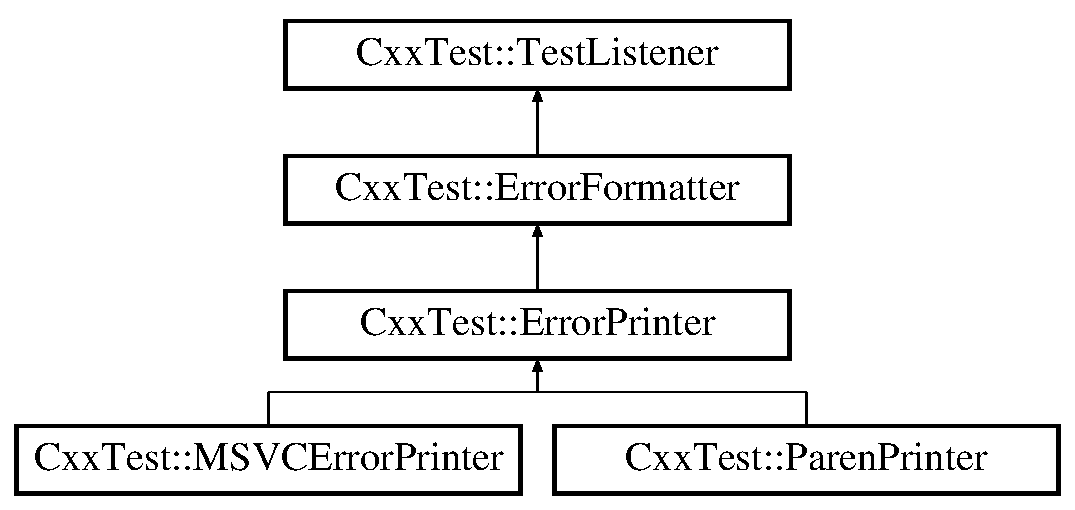
\includegraphics[height=4.000000cm]{classCxxTest_1_1ErrorPrinter}
\end{center}
\end{figure}
\subsection*{Public Member Functions}
\begin{DoxyCompactItemize}
\item 
\hypertarget{classCxxTest_1_1ErrorPrinter_ab51bf2abfd3365f1d120f4c32ff3d8ad}{{\bfseries Error\-Printer} (C\-X\-X\-T\-E\-S\-T\-\_\-\-S\-T\-D(ostream)\&o=C\-X\-X\-T\-E\-S\-T\-\_\-\-S\-T\-D(cout), const char $\ast$pre\-Line=\char`\"{}\-:\char`\"{}, const char $\ast$post\-Line=\char`\"{}\char`\"{}, const char $\ast$error\-String=\char`\"{}Error\char`\"{}, const char $\ast$warning\-String=\char`\"{}Warning\char`\"{})}\label{classCxxTest_1_1ErrorPrinter_ab51bf2abfd3365f1d120f4c32ff3d8ad}

\end{DoxyCompactItemize}
\subsection*{Additional Inherited Members}


The documentation for this class was generated from the following file\-:\begin{DoxyCompactItemize}
\item 
test/cxxtest/cxxtest/Error\-Printer.\-h\end{DoxyCompactItemize}

\hypertarget{classExceptionTest}{\section{Exception\-Test Class Reference}
\label{classExceptionTest}\index{Exception\-Test@{Exception\-Test}}
}
Inheritance diagram for Exception\-Test\-:\begin{figure}[H]
\begin{center}
\leavevmode
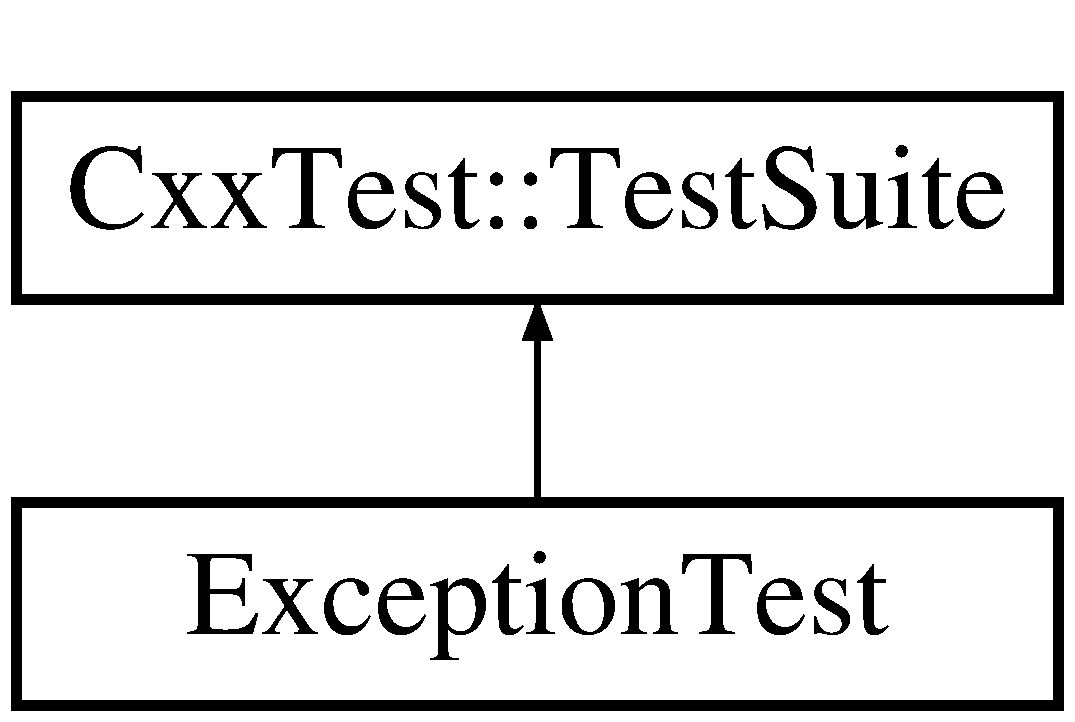
\includegraphics[height=2.000000cm]{classExceptionTest}
\end{center}
\end{figure}
\subsection*{Public Member Functions}
\begin{DoxyCompactItemize}
\item 
\hypertarget{classExceptionTest_a861cc742e3bd0038eaadeab6fb8d921b}{void {\bfseries test\-Assertion} (void)}\label{classExceptionTest_a861cc742e3bd0038eaadeab6fb8d921b}

\end{DoxyCompactItemize}


The documentation for this class was generated from the following file\-:\begin{DoxyCompactItemize}
\item 
test/cxxtest/sample/Exception\-Test.\-h\end{DoxyCompactItemize}

\hypertarget{classFactor}{\section{Factor Class Reference}
\label{classFactor}\index{Factor@{Factor}}
}
Inheritance diagram for Factor\-:\begin{figure}[H]
\begin{center}
\leavevmode
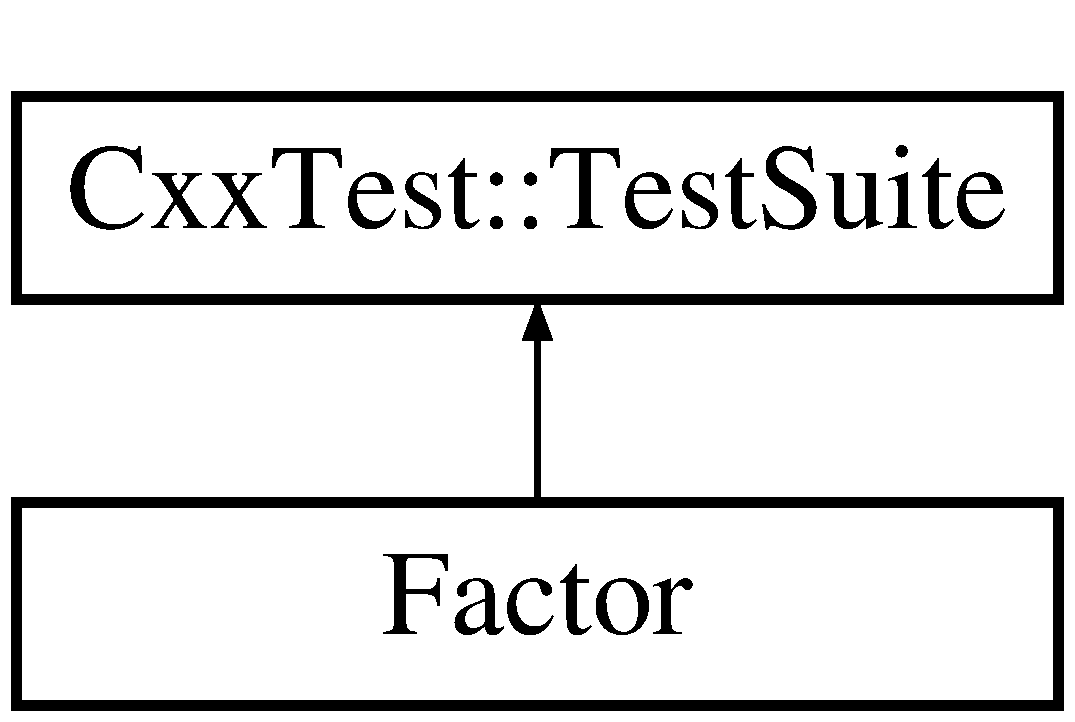
\includegraphics[height=2.000000cm]{classFactor}
\end{center}
\end{figure}
\subsection*{Classes}
\begin{DoxyCompactItemize}
\item 
class \hyperlink{classFactor_1_1NotShorterThan}{Not\-Shorter\-Than}
\item 
class \hyperlink{classFactor_1_1ShorterThan}{Shorter\-Than}
\item 
class \hyperlink{classFactor_1_1X}{X}
\end{DoxyCompactItemize}
\subsection*{Public Types}
\begin{DoxyCompactItemize}
\item 
enum {\bfseries Limit} \{ {\bfseries M\-A\-X\-\_\-\-S\-T\-R\-L\-E\-N\-\_\-\-T\-O\-T\-A\-L\-\_\-\-T\-E\-S\-T\-S} = Cxx\-Test\-:\-:World\-Description\-:\-:M\-A\-X\-\_\-\-S\-T\-R\-L\-E\-N\-\_\-\-T\-O\-T\-A\-L\-\_\-\-T\-E\-S\-T\-S
 \}
\end{DoxyCompactItemize}
\subsection*{Public Member Functions}
\begin{DoxyCompactItemize}
\item 
\hypertarget{classFactor_a7426118def38f980381e4e75c957f379}{const char $\ast$ {\bfseries convert} (unsigned n)}\label{classFactor_a7426118def38f980381e4e75c957f379}

\item 
\hypertarget{classFactor_a16ce4aaaab92583bbf5efb8952c06300}{void {\bfseries test\-\_\-\-Some\-\_\-numbers} ()}\label{classFactor_a16ce4aaaab92583bbf5efb8952c06300}

\item 
\hypertarget{classFactor_a1f67372f5381a94672cdfce3e6e22d38}{void {\bfseries test\-\_\-\-Lengths} ()}\label{classFactor_a1f67372f5381a94672cdfce3e6e22d38}

\end{DoxyCompactItemize}
\subsection*{Public Attributes}
\begin{DoxyCompactItemize}
\item 
\hypertarget{classFactor_a42be44365fe39eda10f1c9fe9f3bd7a9}{\hyperlink{classFactor_1_1X}{X} {\bfseries x}}\label{classFactor_a42be44365fe39eda10f1c9fe9f3bd7a9}

\item 
\hypertarget{classFactor_a4cb12c126492d48d1d1a374962c43617}{char {\bfseries buffer} \mbox{[}M\-A\-X\-\_\-\-S\-T\-R\-L\-E\-N\-\_\-\-T\-O\-T\-A\-L\-\_\-\-T\-E\-S\-T\-S $\ast$2\mbox{]}}\label{classFactor_a4cb12c126492d48d1d1a374962c43617}

\end{DoxyCompactItemize}


The documentation for this class was generated from the following file\-:\begin{DoxyCompactItemize}
\item 
test/cxxtest/test/Factor.\-h\end{DoxyCompactItemize}

\hypertarget{classFail}{\section{Fail Class Reference}
\label{classFail}\index{Fail@{Fail}}
}
\subsection*{Public Member Functions}
\begin{DoxyCompactItemize}
\item 
\hypertarget{classFail_a3ae082e03b5162d873be2790158a98f2}{bool {\bfseries operator()} (int) const }\label{classFail_a3ae082e03b5162d873be2790158a98f2}

\item 
\hypertarget{classFail_ab58704cea84a6eda24d55eea573e6679}{bool {\bfseries operator()} (int, int) const }\label{classFail_ab58704cea84a6eda24d55eea573e6679}

\end{DoxyCompactItemize}


The documentation for this class was generated from the following file\-:\begin{DoxyCompactItemize}
\item 
test/cxxtest/test/Throws\-Assert.\-h\end{DoxyCompactItemize}

\hypertarget{classFBlur}{\section{F\-Blur Class Reference}
\label{classFBlur}\index{F\-Blur@{F\-Blur}}
}
Inheritance diagram for F\-Blur\-:\begin{figure}[H]
\begin{center}
\leavevmode
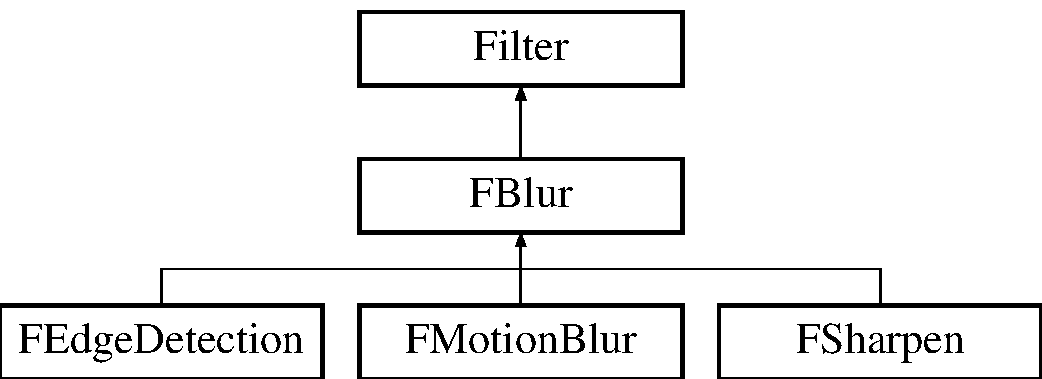
\includegraphics[height=3.000000cm]{classFBlur}
\end{center}
\end{figure}
\subsection*{Public Member Functions}
\begin{DoxyCompactItemize}
\item 
\hypertarget{classFBlur_a20d9f9bb8f2b787273a860779853a8fd}{void {\bfseries apply\-Filter} (\hyperlink{classPixelBuffer}{Pixel\-Buffer} $\ast$image\-Buffer)}\label{classFBlur_a20d9f9bb8f2b787273a860779853a8fd}

\item 
\hypertarget{classFBlur_a3c121581f48e00e0267f88826808ee23}{std\-::string {\bfseries get\-Name} ()}\label{classFBlur_a3c121581f48e00e0267f88826808ee23}

\item 
\hypertarget{classFBlur_ad7d9aa0fa6b3b4f4ead1545ccf6a6628}{virtual kernel\-Type {\bfseries build\-Kernel} (int radius)}\label{classFBlur_ad7d9aa0fa6b3b4f4ead1545ccf6a6628}

\item 
\hypertarget{classFBlur_a97ca2bede17042bae70d781859d46e73}{kernel\-Type {\bfseries box\-Filter} (int radius)}\label{classFBlur_a97ca2bede17042bae70d781859d46e73}

\item 
\hypertarget{classFBlur_ab13f7d8c36423e3f0ecabdcd9b045fbf}{kernel\-Type {\bfseries empty\-Filter} (int radius)}\label{classFBlur_ab13f7d8c36423e3f0ecabdcd9b045fbf}

\item 
\hypertarget{classFBlur_ad88afc728cb9b8c84443a0bf4a30983f}{kernel\-Type {\bfseries Gaussian\-Blur} (float sigma)}\label{classFBlur_ad88afc728cb9b8c84443a0bf4a30983f}

\item 
\hypertarget{classFBlur_a7cb16fe19cd319be83d95de5686e8d39}{kernel\-Type {\bfseries get\-Kernel} ()}\label{classFBlur_a7cb16fe19cd319be83d95de5686e8d39}

\item 
\hypertarget{classFBlur_a5f500e9bad040039fb43e58be03d57e6}{void {\bfseries print\-Kernel} ()}\label{classFBlur_a5f500e9bad040039fb43e58be03d57e6}

\end{DoxyCompactItemize}


The documentation for this class was generated from the following files\-:\begin{DoxyCompactItemize}
\item 
libphoto/F\-Blur.\-h\item 
libphoto/F\-Blur.\-cpp\end{DoxyCompactItemize}

\hypertarget{classFChannel}{}\section{F\+Channel Class Reference}
\label{classFChannel}\index{F\+Channel@{F\+Channel}}
Inheritance diagram for F\+Channel\+:\begin{figure}[H]
\begin{center}
\leavevmode
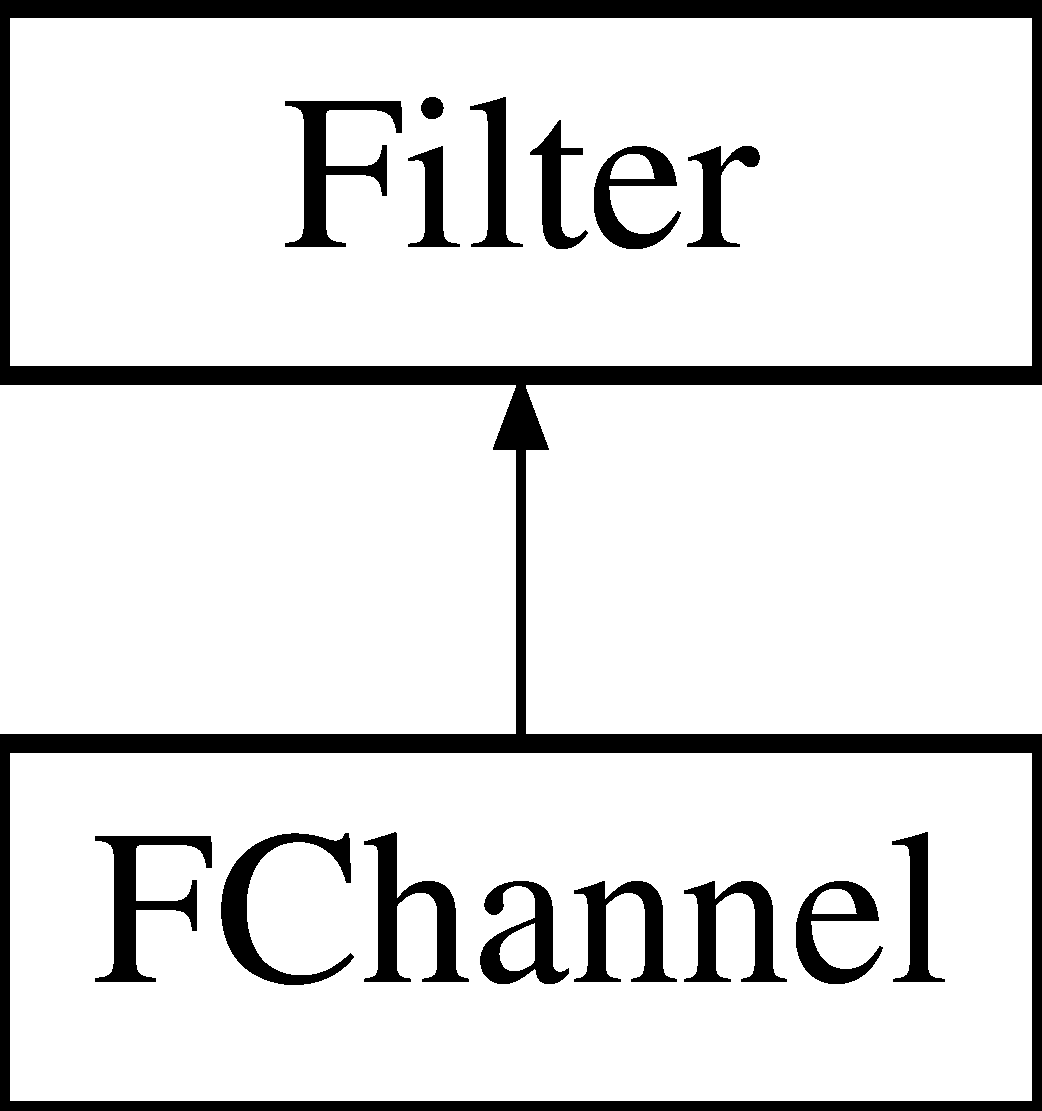
\includegraphics[height=2.000000cm]{classFChannel}
\end{center}
\end{figure}
\subsection*{Public Member Functions}
\begin{DoxyCompactItemize}
\item 
\hyperlink{classFChannel_acc91e001fcac19d758179c410e75be7a}{F\+Channel} ()
\item 
void \hyperlink{classFChannel_a74a786921c11b3d82119b74f05d3d0c0}{apply\+Filter} (\hyperlink{classPixelBuffer}{Pixel\+Buffer} $\ast$image\+Buffer)\hypertarget{classFChannel_a74a786921c11b3d82119b74f05d3d0c0}{}\label{classFChannel_a74a786921c11b3d82119b74f05d3d0c0}

\begin{DoxyCompactList}\small\item\em apply channel filter effect to the Pixel\+Buffer$\ast$ buffer passed into this function \end{DoxyCompactList}\item 
std\+::string \hyperlink{classFChannel_a3d7618565e8643f1a4f87d12a968e406}{get\+Name} ()\hypertarget{classFChannel_a3d7618565e8643f1a4f87d12a968e406}{}\label{classFChannel_a3d7618565e8643f1a4f87d12a968e406}

\begin{DoxyCompactList}\small\item\em get class name for filter \end{DoxyCompactList}\end{DoxyCompactItemize}


\subsection{Constructor \& Destructor Documentation}
\index{F\+Channel@{F\+Channel}!F\+Channel@{F\+Channel}}
\index{F\+Channel@{F\+Channel}!F\+Channel@{F\+Channel}}
\subsubsection[{\texorpdfstring{F\+Channel()}{FChannel()}}]{\setlength{\rightskip}{0pt plus 5cm}F\+Channel\+::\+F\+Channel (
\begin{DoxyParamCaption}
{}
\end{DoxyParamCaption}
)}\hypertarget{classFChannel_acc91e001fcac19d758179c410e75be7a}{}\label{classFChannel_acc91e001fcac19d758179c410e75be7a}
This is the \hyperlink{classFChannel}{F\+Channel} class, it is used for all the channel image filters . apply\+Filter describes how this filter will be applied to every pixel in the image. 

The documentation for this class was generated from the following files\+:\begin{DoxyCompactItemize}
\item 
libphoto/F\+Channel.\+h\item 
libphoto/F\+Channel.\+cpp\end{DoxyCompactItemize}

\hypertarget{classFEdgeDetection}{\section{F\-Edge\-Detection Class Reference}
\label{classFEdgeDetection}\index{F\-Edge\-Detection@{F\-Edge\-Detection}}
}
Inheritance diagram for F\-Edge\-Detection\-:\begin{figure}[H]
\begin{center}
\leavevmode
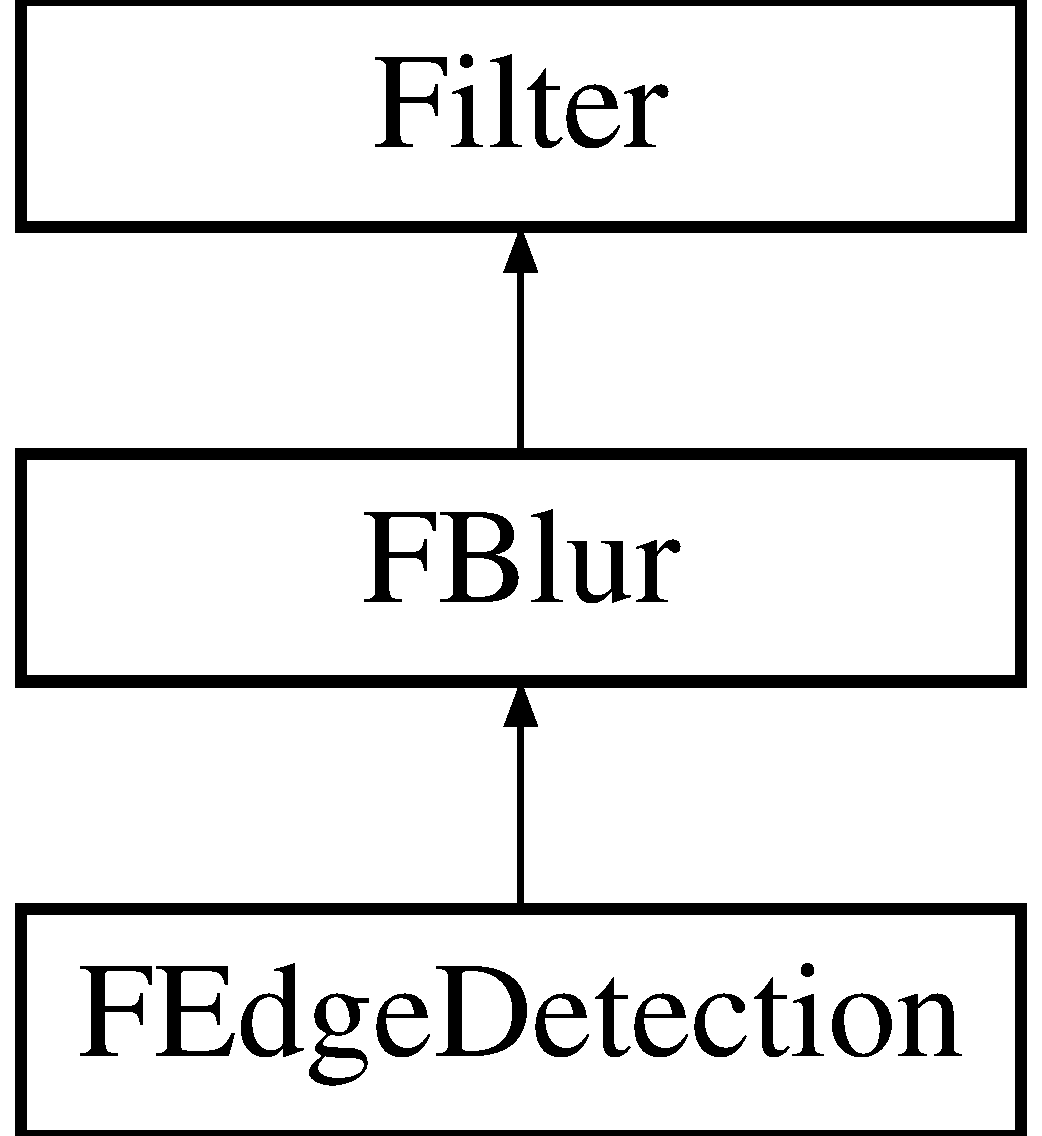
\includegraphics[height=4.242424cm]{classFEdgeDetection}
\end{center}
\end{figure}
\subsection*{Public Member Functions}
\begin{DoxyCompactItemize}
\item 
\hypertarget{classFEdgeDetection_acdf7ec56e2f1f5010b84ebcd66a958f3}{std\-::string {\bfseries get\-Name} ()}\label{classFEdgeDetection_acdf7ec56e2f1f5010b84ebcd66a958f3}

\item 
\hypertarget{classFEdgeDetection_a58c541bf60eb4e21bdb656bdad5f8c65}{kernel\-Type {\bfseries build\-Kernel} (int radius)}\label{classFEdgeDetection_a58c541bf60eb4e21bdb656bdad5f8c65}

\item 
\hypertarget{classFEdgeDetection_acdf7ec56e2f1f5010b84ebcd66a958f3}{std\-::string {\bfseries get\-Name} ()}\label{classFEdgeDetection_acdf7ec56e2f1f5010b84ebcd66a958f3}

\item 
\hypertarget{classFEdgeDetection_a58c541bf60eb4e21bdb656bdad5f8c65}{kernel\-Type {\bfseries build\-Kernel} (int radius)}\label{classFEdgeDetection_a58c541bf60eb4e21bdb656bdad5f8c65}

\item 
\hypertarget{classFEdgeDetection_acdf7ec56e2f1f5010b84ebcd66a958f3}{std\-::string {\bfseries get\-Name} ()}\label{classFEdgeDetection_acdf7ec56e2f1f5010b84ebcd66a958f3}

\item 
\hypertarget{classFEdgeDetection_a58c541bf60eb4e21bdb656bdad5f8c65}{kernel\-Type {\bfseries build\-Kernel} (int radius)}\label{classFEdgeDetection_a58c541bf60eb4e21bdb656bdad5f8c65}

\end{DoxyCompactItemize}
\subsection*{Additional Inherited Members}


The documentation for this class was generated from the following files\-:\begin{DoxyCompactItemize}
\item 
libphoto/F\-Edge\-Detection.\-h\item 
libphoto/include/libphoto.\-h\item 
libphoto/F\-Edge\-Detection.\-cpp\end{DoxyCompactItemize}

\hypertarget{classFillTool}{\section{Fill\-Tool Class Reference}
\label{classFillTool}\index{Fill\-Tool@{Fill\-Tool}}
}
Inheritance diagram for Fill\-Tool\-:\begin{figure}[H]
\begin{center}
\leavevmode
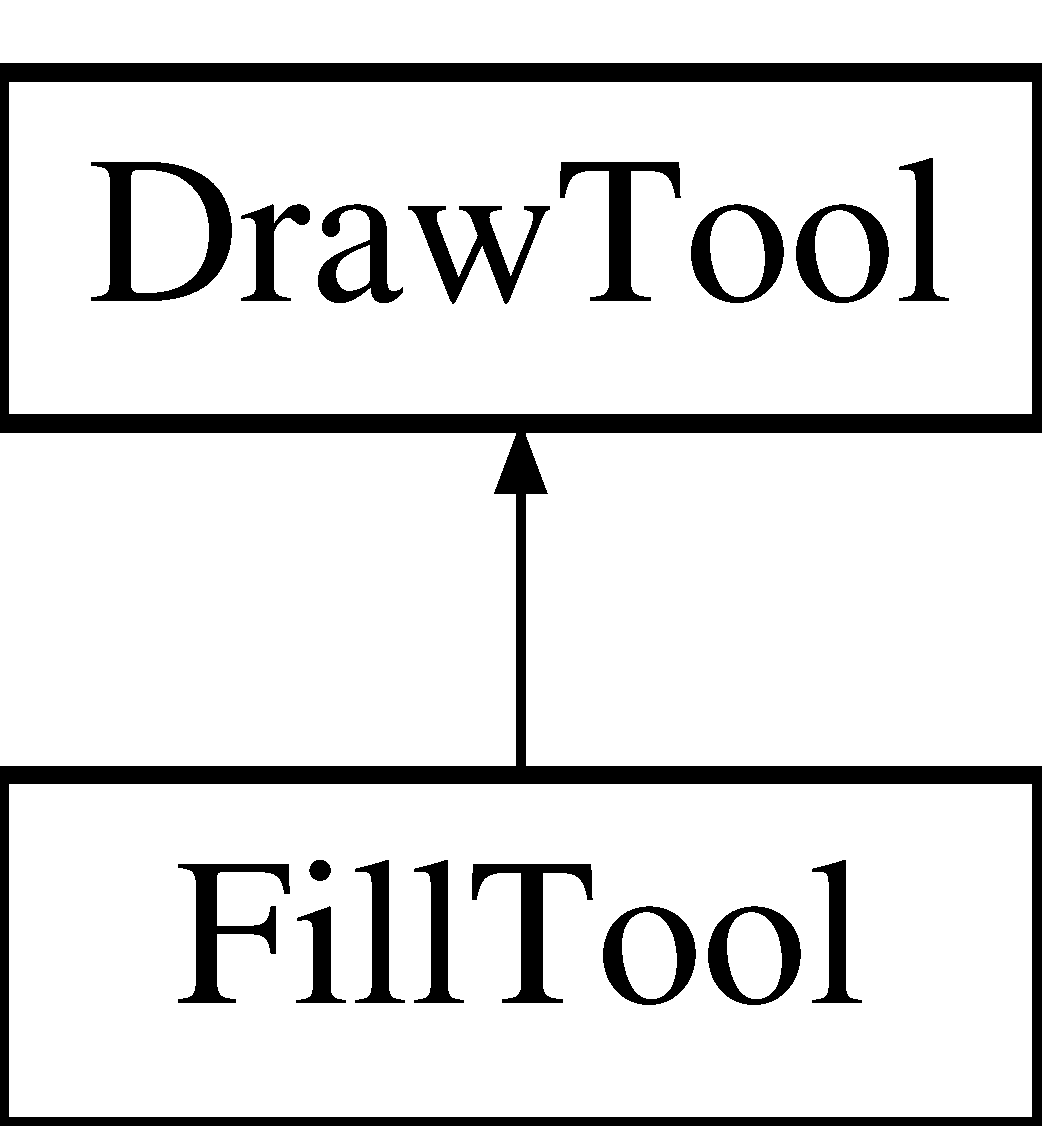
\includegraphics[height=2.000000cm]{classFillTool}
\end{center}
\end{figure}
\subsection*{Public Member Functions}
\begin{DoxyCompactItemize}
\item 
\hypertarget{classFillTool_a6abe3f5032f5e69a11cf38b94da90a62}{{\bfseries Fill\-Tool} (\hyperlink{classColorData}{Color\-Data} $\ast$tool\-Color, int height, int width)}\label{classFillTool_a6abe3f5032f5e69a11cf38b94da90a62}

\item 
\hypertarget{classFillTool_a81a3a46e5600d6250634766e8b769796}{void {\bfseries paint} (int x, int y, int prev\-X, int prev\-Y, \hyperlink{classPixelBuffer}{Pixel\-Buffer} $\ast$buffer)}\label{classFillTool_a81a3a46e5600d6250634766e8b769796}

\item 
\hypertarget{classFillTool_a8ad4d0d5b2a5379be3720c89a102ddb3}{void {\bfseries apply\-Influence} (int x, int y, \hyperlink{classPixelBuffer}{Pixel\-Buffer} $\ast$buffer)}\label{classFillTool_a8ad4d0d5b2a5379be3720c89a102ddb3}

\item 
\hypertarget{classFillTool_a888fd877cf0937e9b36be2d56f06de3e}{void {\bfseries fill\-Influence} ()}\label{classFillTool_a888fd877cf0937e9b36be2d56f06de3e}

\item 
\hypertarget{classFillTool_a6abe3f5032f5e69a11cf38b94da90a62}{{\bfseries Fill\-Tool} (\hyperlink{classColorData}{Color\-Data} $\ast$tool\-Color, int height, int width)}\label{classFillTool_a6abe3f5032f5e69a11cf38b94da90a62}

\item 
\hypertarget{classFillTool_a81a3a46e5600d6250634766e8b769796}{void {\bfseries paint} (int x, int y, int prev\-X, int prev\-Y, \hyperlink{classPixelBuffer}{Pixel\-Buffer} $\ast$buffer)}\label{classFillTool_a81a3a46e5600d6250634766e8b769796}

\item 
\hypertarget{classFillTool_a8ad4d0d5b2a5379be3720c89a102ddb3}{void {\bfseries apply\-Influence} (int x, int y, \hyperlink{classPixelBuffer}{Pixel\-Buffer} $\ast$buffer)}\label{classFillTool_a8ad4d0d5b2a5379be3720c89a102ddb3}

\item 
\hypertarget{classFillTool_a888fd877cf0937e9b36be2d56f06de3e}{void {\bfseries fill\-Influence} ()}\label{classFillTool_a888fd877cf0937e9b36be2d56f06de3e}

\item 
\hypertarget{classFillTool_a6abe3f5032f5e69a11cf38b94da90a62}{{\bfseries Fill\-Tool} (\hyperlink{classColorData}{Color\-Data} $\ast$tool\-Color, int height, int width)}\label{classFillTool_a6abe3f5032f5e69a11cf38b94da90a62}

\item 
\hypertarget{classFillTool_a81a3a46e5600d6250634766e8b769796}{void {\bfseries paint} (int x, int y, int prev\-X, int prev\-Y, \hyperlink{classPixelBuffer}{Pixel\-Buffer} $\ast$buffer)}\label{classFillTool_a81a3a46e5600d6250634766e8b769796}

\item 
\hypertarget{classFillTool_a8ad4d0d5b2a5379be3720c89a102ddb3}{void {\bfseries apply\-Influence} (int x, int y, \hyperlink{classPixelBuffer}{Pixel\-Buffer} $\ast$buffer)}\label{classFillTool_a8ad4d0d5b2a5379be3720c89a102ddb3}

\item 
\hypertarget{classFillTool_a888fd877cf0937e9b36be2d56f06de3e}{void {\bfseries fill\-Influence} ()}\label{classFillTool_a888fd877cf0937e9b36be2d56f06de3e}

\end{DoxyCompactItemize}
\subsection*{Additional Inherited Members}


The documentation for this class was generated from the following files\-:\begin{DoxyCompactItemize}
\item 
libphoto/Fill\-Tool.\-h\item 
libphoto/include/libphoto.\-h\item 
libphoto/Fill\-Tool.\-cpp\end{DoxyCompactItemize}

\hypertarget{classFilter}{\section{Filter Class Reference}
\label{classFilter}\index{Filter@{Filter}}
}
Inheritance diagram for Filter\-:\begin{figure}[H]
\begin{center}
\leavevmode
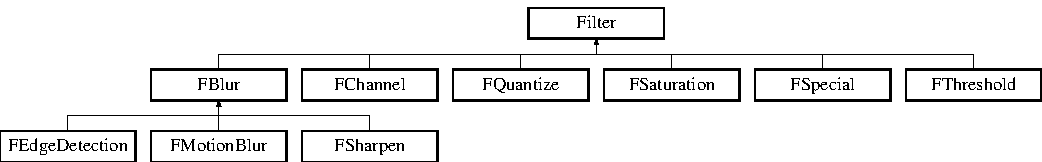
\includegraphics[height=2.181818cm]{classFilter}
\end{center}
\end{figure}
\subsection*{Public Member Functions}
\begin{DoxyCompactItemize}
\item 
\hypertarget{classFilter_a2ecb4bc0e81851d30f46f30bf81d1739}{virtual void {\bfseries apply\-Filter} (\hyperlink{classPixelBuffer}{Pixel\-Buffer} $\ast$image\-Buffer)=0}\label{classFilter_a2ecb4bc0e81851d30f46f30bf81d1739}

\item 
\hypertarget{classFilter_a212f40acb6481b2e36c3d129007519f1}{virtual std\-::string {\bfseries get\-Name} ()=0}\label{classFilter_a212f40acb6481b2e36c3d129007519f1}

\item 
\hypertarget{classFilter_aba015e9da647ba41fee4b41019d54516}{virtual void {\bfseries set\-Filter\-Parameter} (float parameter)}\label{classFilter_aba015e9da647ba41fee4b41019d54516}

\item 
\hypertarget{classFilter_a88314088e678c9a7cdbe0d0557385fa8}{virtual void {\bfseries set\-Filter\-Parameter} (\hyperlink{classColorData}{Color\-Data} parameter)}\label{classFilter_a88314088e678c9a7cdbe0d0557385fa8}

\item 
\hypertarget{classFilter_ada9d5f112e217c9bcf413093eae2a1e9}{void {\bfseries set\-Blur\-Direction} (int direction)}\label{classFilter_ada9d5f112e217c9bcf413093eae2a1e9}

\item 
\hypertarget{classFilter_a9f741b045bf1d57e485f116ce62ebac1}{float {\bfseries get\-Float\-Parameter} ()}\label{classFilter_a9f741b045bf1d57e485f116ce62ebac1}

\item 
\hypertarget{classFilter_abf85cdf0cda6dbe1dbcd6b8813aeecf3}{\hyperlink{classColorData}{Color\-Data} {\bfseries get\-Color\-Parameter} ()}\label{classFilter_abf85cdf0cda6dbe1dbcd6b8813aeecf3}

\item 
\hypertarget{classFilter_a465a168fc580c773e58d4df2f3db5968}{int {\bfseries get\-Blur\-Diection} ()}\label{classFilter_a465a168fc580c773e58d4df2f3db5968}

\end{DoxyCompactItemize}
\subsection*{Private Attributes}
\begin{DoxyCompactItemize}
\item 
\hypertarget{classFilter_a9bd610a1db8e1cde51f78b3a01b6638c}{float {\bfseries f\-\_\-parameter}}\label{classFilter_a9bd610a1db8e1cde51f78b3a01b6638c}

\item 
\hypertarget{classFilter_ab5464736d6dcb521cb14ac147f68ad7e}{\hyperlink{classColorData}{Color\-Data} {\bfseries c\-\_\-parameter}}\label{classFilter_ab5464736d6dcb521cb14ac147f68ad7e}

\item 
\hypertarget{classFilter_a05e0243ffe83143ba6c85084824be510}{int {\bfseries blur\-Direction}}\label{classFilter_a05e0243ffe83143ba6c85084824be510}

\end{DoxyCompactItemize}


The documentation for this class was generated from the following file\-:\begin{DoxyCompactItemize}
\item 
libphoto/Filter.\-h\end{DoxyCompactItemize}

\hypertarget{classFilterFactory}{\section{Filter\-Factory Class Reference}
\label{classFilterFactory}\index{Filter\-Factory@{Filter\-Factory}}
}
\subsection*{Public Types}
\begin{DoxyCompactItemize}
\item 
enum {\bfseries F\-I\-L\-T\-E\-R\-S} \{ \\*
{\bfseries F\-I\-L\-T\-E\-R\-\_\-\-T\-H\-R\-E\-S\-H\-O\-L\-D} = 0, 
{\bfseries F\-I\-L\-T\-E\-R\-\_\-\-C\-H\-A\-N\-N\-E\-L} = 1, 
{\bfseries F\-I\-L\-T\-E\-R\-\_\-\-S\-A\-T\-U\-R\-A\-T\-I\-O\-N} = 2, 
{\bfseries F\-I\-L\-T\-E\-R\-\_\-\-Q\-U\-A\-N\-T\-I\-Z\-E} = 3, 
\\*
{\bfseries F\-I\-L\-T\-E\-R\-\_\-\-B\-L\-U\-R} = 4, 
{\bfseries F\-I\-L\-T\-E\-R\-\_\-\-M\-O\-T\-I\-O\-N\-\_\-\-B\-L\-U\-R} = 5, 
{\bfseries F\-I\-L\-T\-E\-R\-\_\-\-S\-H\-A\-R\-P\-E\-N} = 6, 
{\bfseries F\-I\-L\-T\-E\-R\-\_\-\-D\-E\-T\-E\-C\-T\-\_\-\-E\-D\-G\-E\-S} = 7, 
\\*
{\bfseries F\-I\-L\-T\-E\-R\-\_\-\-S\-P\-E\-C\-I\-A\-L} = 8, 
{\bfseries N\-U\-M\-F\-I\-L\-T\-E\-R\-S} = 9
 \}
\end{DoxyCompactItemize}
\subsection*{Static Public Member Functions}
\begin{DoxyCompactItemize}
\item 
static int \hyperlink{classFilterFactory_a978466237a3acfbd5570fbf1d4dc1080}{get\-Num\-Filters} ()
\item 
static \hyperlink{classFilter}{Filter} $\ast$ \hyperlink{classFilterFactory_afa9986fc11ea262c26febc9191a19f47}{create\-Filter} (int filter\-I\-D)
\end{DoxyCompactItemize}


\subsection{Member Function Documentation}
\hypertarget{classFilterFactory_afa9986fc11ea262c26febc9191a19f47}{\index{Filter\-Factory@{Filter\-Factory}!create\-Filter@{create\-Filter}}
\index{create\-Filter@{create\-Filter}!FilterFactory@{Filter\-Factory}}
\subsubsection[{create\-Filter}]{\setlength{\rightskip}{0pt plus 5cm}{\bf Filter} $\ast$ Filter\-Factory\-::create\-Filter (
\begin{DoxyParamCaption}
\item[{int}]{filter\-I\-D}
\end{DoxyParamCaption}
)\hspace{0.3cm}{\ttfamily [static]}}}\label{classFilterFactory_afa9986fc11ea262c26febc9191a19f47}
Creates a filter for the given I\-D \par
param filter\-I\-D which filter you want to created \par
 return a filter instance \par
\hypertarget{classFilterFactory_a978466237a3acfbd5570fbf1d4dc1080}{\index{Filter\-Factory@{Filter\-Factory}!get\-Num\-Filters@{get\-Num\-Filters}}
\index{get\-Num\-Filters@{get\-Num\-Filters}!FilterFactory@{Filter\-Factory}}
\subsubsection[{get\-Num\-Filters}]{\setlength{\rightskip}{0pt plus 5cm}int Filter\-Factory\-::get\-Num\-Filters (
\begin{DoxyParamCaption}
{}
\end{DoxyParamCaption}
)\hspace{0.3cm}{\ttfamily [static]}}}\label{classFilterFactory_a978466237a3acfbd5570fbf1d4dc1080}
This is the \hyperlink{classFilterFactory}{Filter\-Factory} class, it is used to control the selection logic for filters. 

The documentation for this class was generated from the following files\-:\begin{DoxyCompactItemize}
\item 
libphoto/Filter\-Factory.\-h\item 
libphoto/Filter\-Factory.\-cpp\end{DoxyCompactItemize}

\hypertarget{classFilterToolTest}{\section{Filter\-Tool\-Test Class Reference}
\label{classFilterToolTest}\index{Filter\-Tool\-Test@{Filter\-Tool\-Test}}
}
Inheritance diagram for Filter\-Tool\-Test\-:\begin{figure}[H]
\begin{center}
\leavevmode
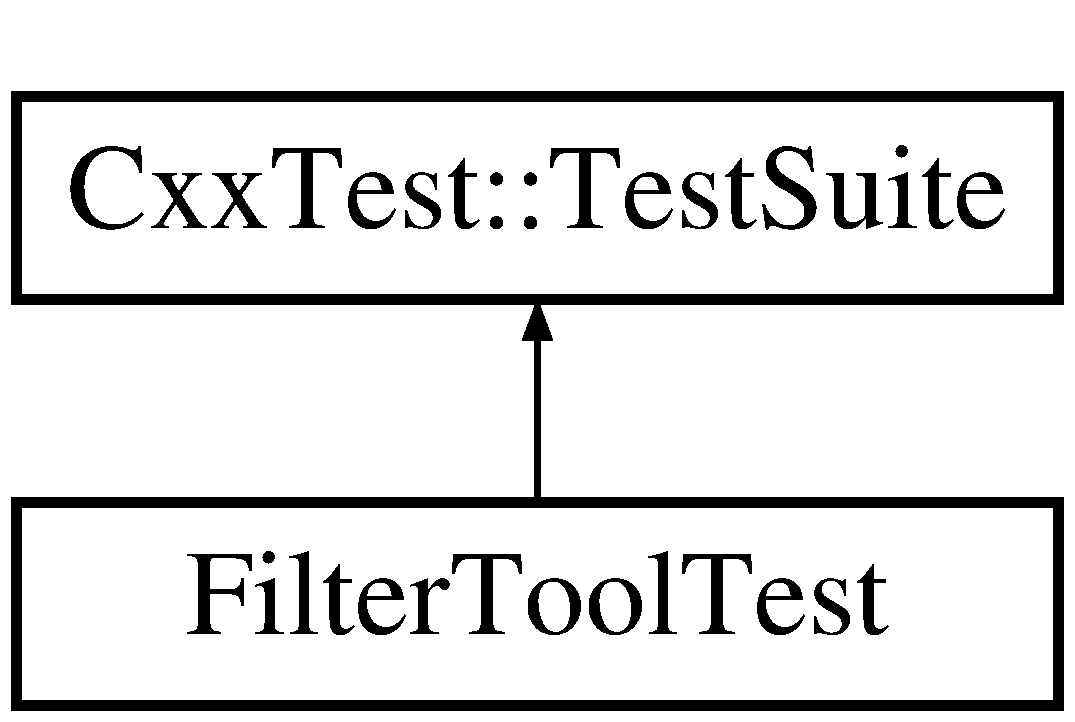
\includegraphics[height=2.000000cm]{classFilterToolTest}
\end{center}
\end{figure}
\subsection*{Public Member Functions}
\begin{DoxyCompactItemize}
\item 
\hypertarget{classFilterToolTest_a7118243f3c0cbbeeaa63afa2a28afbdb}{void {\bfseries set\-Up} ()}\label{classFilterToolTest_a7118243f3c0cbbeeaa63afa2a28afbdb}

\item 
\hypertarget{classFilterToolTest_a504ad5f4dff73d0d28174aeb4579e7be}{void {\bfseries tear\-Down} ()}\label{classFilterToolTest_a504ad5f4dff73d0d28174aeb4579e7be}

\item 
\hypertarget{classFilterToolTest_a11ecc9ffbaea30b9b614b0eb0b9e6809}{\hyperlink{classPixelBuffer}{Pixel\-Buffer} $\ast$ {\bfseries read\-File} (string file\-Path)}\label{classFilterToolTest_a11ecc9ffbaea30b9b614b0eb0b9e6809}

\item 
\hypertarget{classFilterToolTest_abf87ae201ad787773d9dc5b21813e0d3}{string {\bfseries get\-Input\-File} ()}\label{classFilterToolTest_abf87ae201ad787773d9dc5b21813e0d3}

\item 
\hypertarget{classFilterToolTest_a711c3299ced93a3a997efa5caca6138d}{string {\bfseries get\-Output\-File} (string file\-Name)}\label{classFilterToolTest_a711c3299ced93a3a997efa5caca6138d}

\item 
\hypertarget{classFilterToolTest_a7197998e31e539b21b150471dfca6f9d}{string {\bfseries get\-Verify\-File} (string file\-Name)}\label{classFilterToolTest_a7197998e31e539b21b150471dfca6f9d}

\item 
\hypertarget{classFilterToolTest_a1fa65c57dc84ed19daccdfea6361a33f}{void {\bfseries test\-Edge\-Detection} ()}\label{classFilterToolTest_a1fa65c57dc84ed19daccdfea6361a33f}

\item 
\hypertarget{classFilterToolTest_add51010398df3f598487eecfd7670a20}{void {\bfseries test\-Output\-File} (string file, string output\-File)}\label{classFilterToolTest_add51010398df3f598487eecfd7670a20}

\item 
\hypertarget{classFilterToolTest_ab8489f7e7d0c309e66d967dba2cb4df4}{void {\bfseries test\-Threshold} ()}\label{classFilterToolTest_ab8489f7e7d0c309e66d967dba2cb4df4}

\item 
\hypertarget{classFilterToolTest_adabbe17ffd24e96bac9325aae26f0bec}{void {\bfseries test\-Channel} ()}\label{classFilterToolTest_adabbe17ffd24e96bac9325aae26f0bec}

\item 
\hypertarget{classFilterToolTest_a53287d0faff3bd9f9aedbf63932bae5b}{void {\bfseries test\-Sharpen} ()}\label{classFilterToolTest_a53287d0faff3bd9f9aedbf63932bae5b}

\item 
\hypertarget{classFilterToolTest_a1c3a6255cd347a6d0f8c0c2a8861049f}{void {\bfseries test\-Saturate} ()}\label{classFilterToolTest_a1c3a6255cd347a6d0f8c0c2a8861049f}

\item 
\hypertarget{classFilterToolTest_a43df374e5b3f8afe37f6fed5f050a24b}{void {\bfseries test\-Quantize} ()}\label{classFilterToolTest_a43df374e5b3f8afe37f6fed5f050a24b}

\item 
\hypertarget{classFilterToolTest_ab197f7ffabec25281958197f5e2e151c}{void {\bfseries test\-Special} ()}\label{classFilterToolTest_ab197f7ffabec25281958197f5e2e151c}

\item 
\hypertarget{classFilterToolTest_adbc93011a3919b7c138fabbd699173fb}{void {\bfseries test\-Blur} ()}\label{classFilterToolTest_adbc93011a3919b7c138fabbd699173fb}

\item 
\hypertarget{classFilterToolTest_a967cee9488c62b6e853ca2e543f6ef96}{void {\bfseries test\-M\-Blur\-North\-South} ()}\label{classFilterToolTest_a967cee9488c62b6e853ca2e543f6ef96}

\item 
\hypertarget{classFilterToolTest_a2c322bdb77ccc76be3ac5b94d5386db5}{void {\bfseries test\-M\-Blur\-West\-East} ()}\label{classFilterToolTest_a2c322bdb77ccc76be3ac5b94d5386db5}

\item 
\hypertarget{classFilterToolTest_a009f824d289904d6c357615090a57b2b}{void {\bfseries test\-M\-Blur\-N\-E\-\_\-\-S\-W} ()}\label{classFilterToolTest_a009f824d289904d6c357615090a57b2b}

\item 
\hypertarget{classFilterToolTest_a0ae23dd21aef9d5731176b8269065205}{void {\bfseries test\-M\-Blur\-N\-W\-\_\-\-S\-E} ()}\label{classFilterToolTest_a0ae23dd21aef9d5731176b8269065205}

\end{DoxyCompactItemize}
\subsection*{Public Attributes}
\begin{DoxyCompactItemize}
\item 
\hypertarget{classFilterToolTest_a4e930ca47e70a7590fbcc6928ff3646f}{\hyperlink{classImageHandler}{Image\-Handler} $\ast$ {\bfseries image\-Loader}}\label{classFilterToolTest_a4e930ca47e70a7590fbcc6928ff3646f}

\item 
\hypertarget{classFilterToolTest_a0e07e2b9e93ee95c13b40e647b442f92}{string {\bfseries input\-Prefix} = \char`\"{}input\char`\"{}}\label{classFilterToolTest_a0e07e2b9e93ee95c13b40e647b442f92}

\item 
\hypertarget{classFilterToolTest_a0c4953ea2ad21dfad714233f7c62a402}{string {\bfseries output\-Prefix} = \char`\"{}output\char`\"{}}\label{classFilterToolTest_a0c4953ea2ad21dfad714233f7c62a402}

\item 
\hypertarget{classFilterToolTest_ad302be4e310ea8f6dee6a9e1be72f654}{string {\bfseries verify\-Prefix} = \char`\"{}verify\char`\"{}}\label{classFilterToolTest_ad302be4e310ea8f6dee6a9e1be72f654}

\item 
\hypertarget{classFilterToolTest_a092ca517cd61c8921950193657ea3a1a}{string {\bfseries png\-File} = \char`\"{}water.\-png\char`\"{}}\label{classFilterToolTest_a092ca517cd61c8921950193657ea3a1a}

\item 
\hypertarget{classFilterToolTest_a9d52fc74910157a1fdbb9b385e6e4d2a}{string {\bfseries jpg\-File} = \char`\"{}water.\-jpg\char`\"{}}\label{classFilterToolTest_a9d52fc74910157a1fdbb9b385e6e4d2a}

\item 
\hypertarget{classFilterToolTest_a51daa1e52565ece097b9f8c646b93823}{string {\bfseries delimiter} = \char`\"{}/\char`\"{}}\label{classFilterToolTest_a51daa1e52565ece097b9f8c646b93823}

\item 
\hypertarget{classFilterToolTest_a60811ae01a8e38ada03c91781bcb4d7b}{string {\bfseries redirect\-To\-File} = \char`\"{} $>$ output/test\char`\"{}}\label{classFilterToolTest_a60811ae01a8e38ada03c91781bcb4d7b}

\item 
\hypertarget{classFilterToolTest_a13ec6af4a2cf388c7296c1d7acb2b41f}{string {\bfseries test\-File} = \char`\"{}output/test\char`\"{}}\label{classFilterToolTest_a13ec6af4a2cf388c7296c1d7acb2b41f}

\item 
\hypertarget{classFilterToolTest_a884222e7a8b6b990bf84793e212a9df9}{int {\bfseries height}}\label{classFilterToolTest_a884222e7a8b6b990bf84793e212a9df9}

\item 
\hypertarget{classFilterToolTest_abf9277c4c4257ed1499f304532d039a0}{int {\bfseries width}}\label{classFilterToolTest_abf9277c4c4257ed1499f304532d039a0}

\item 
\hypertarget{classFilterToolTest_a849cbf0cc7c5643cf6d1d4ed7cc8c700}{\hyperlink{classColorData}{Color\-Data} {\bfseries background\-Color}}\label{classFilterToolTest_a849cbf0cc7c5643cf6d1d4ed7cc8c700}

\end{DoxyCompactItemize}


The documentation for this class was generated from the following file\-:\begin{DoxyCompactItemize}
\item 
test/src/Filter\-Tool\-Test.\-h\end{DoxyCompactItemize}

\hypertarget{classFirstSuite}{\section{First\-Suite Class Reference}
\label{classFirstSuite}\index{First\-Suite@{First\-Suite}}
}
Inheritance diagram for First\-Suite\-:\begin{figure}[H]
\begin{center}
\leavevmode
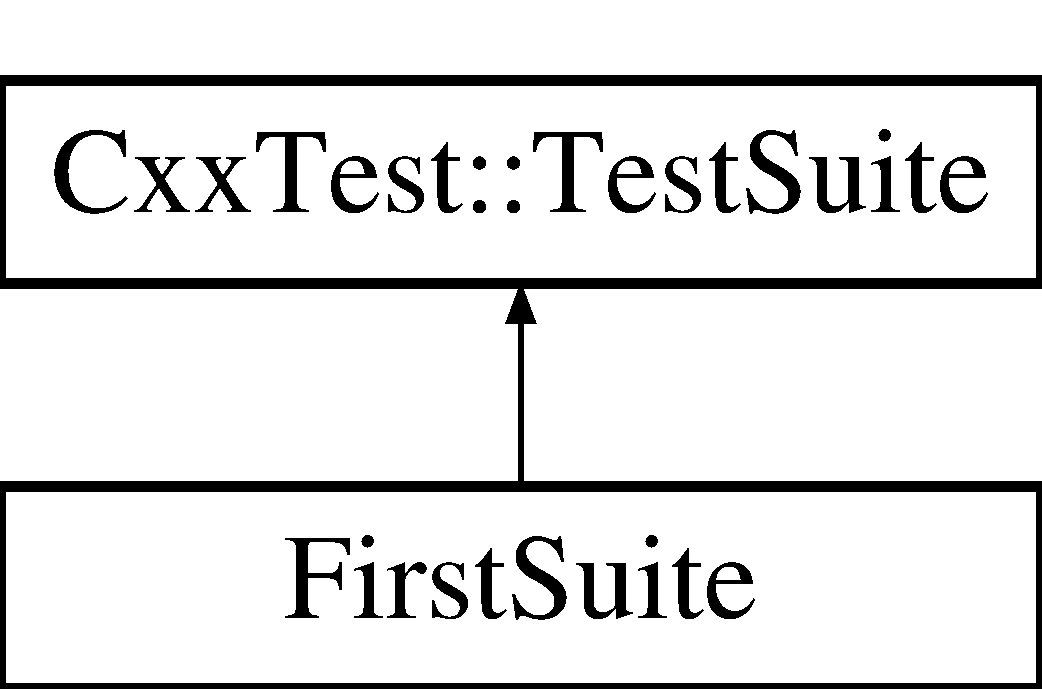
\includegraphics[height=2.000000cm]{classFirstSuite}
\end{center}
\end{figure}
\subsection*{Public Member Functions}
\begin{DoxyCompactItemize}
\item 
\hypertarget{classFirstSuite_a445fdb20f8d37d26f49cee8cc2671c67}{void {\bfseries test\-One} ()}\label{classFirstSuite_a445fdb20f8d37d26f49cee8cc2671c67}

\item 
\hypertarget{classFirstSuite_a734ffa5d1859dbf95ffbca912f88e15f}{void {\bfseries test\-Two} ()}\label{classFirstSuite_a734ffa5d1859dbf95ffbca912f88e15f}

\end{DoxyCompactItemize}


The documentation for this class was generated from the following file\-:\begin{DoxyCompactItemize}
\item 
test/cxxtest/test/World\-Fixtures.\-h\end{DoxyCompactItemize}

\hypertarget{classFixture}{\section{Fixture Class Reference}
\label{classFixture}\index{Fixture@{Fixture}}
}
Inheritance diagram for Fixture\-:\begin{figure}[H]
\begin{center}
\leavevmode
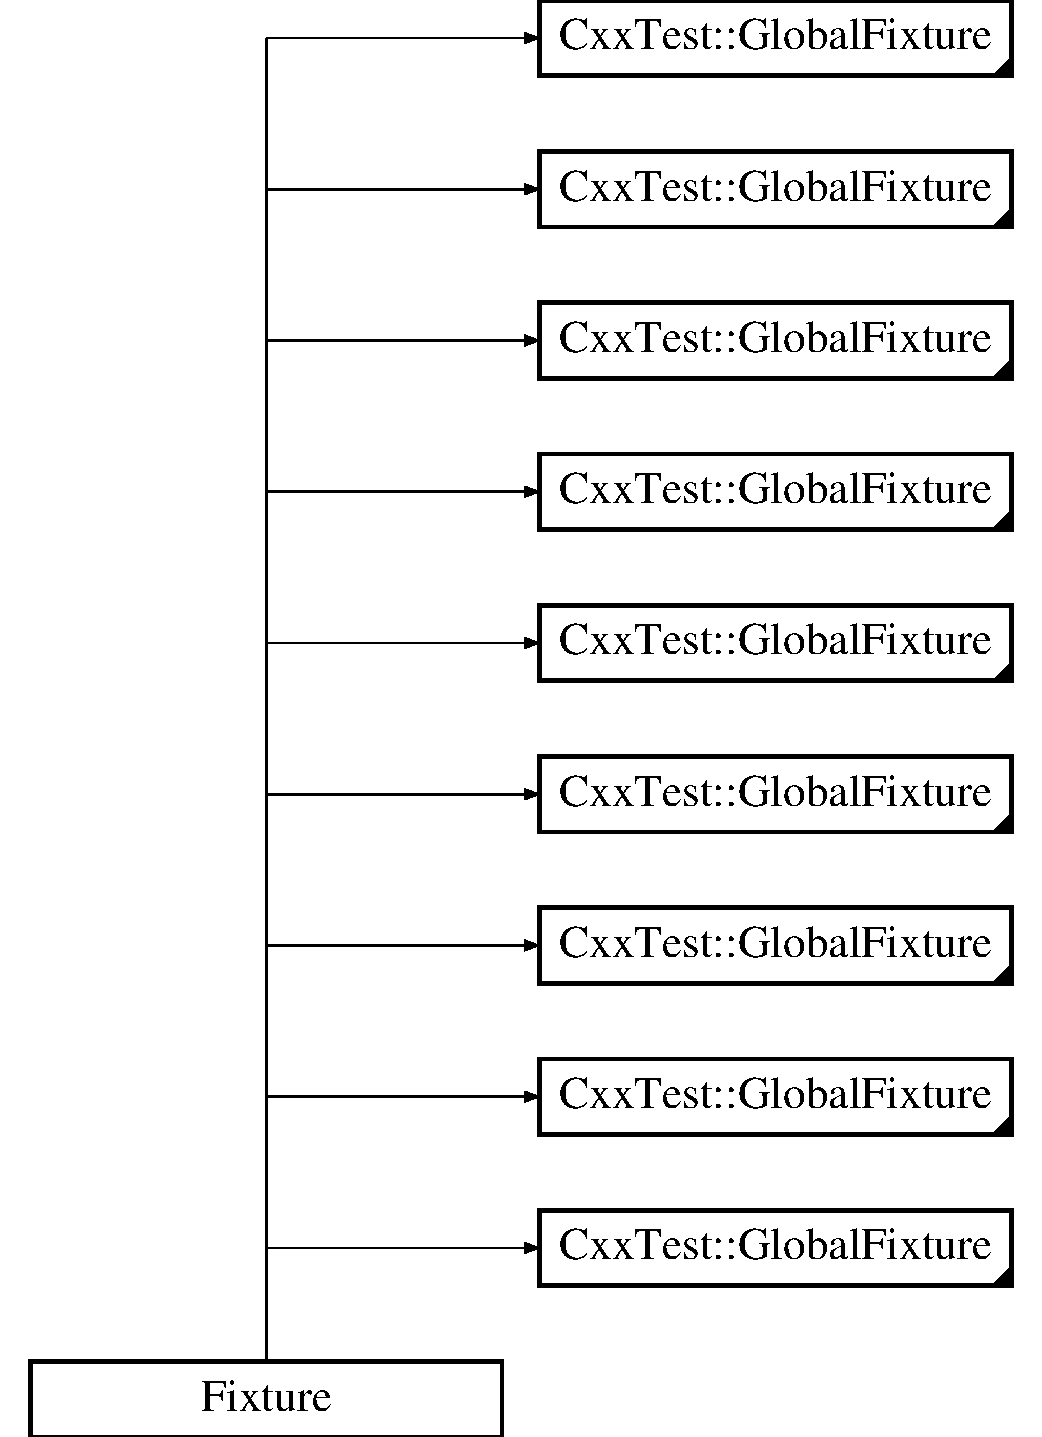
\includegraphics[height=10.000000cm]{classFixture}
\end{center}
\end{figure}
\subsection*{Public Member Functions}
\begin{DoxyCompactItemize}
\item 
\hypertarget{classFixture_ab00b62453dafa5413184465540e5b486}{bool {\bfseries set\-Up} ()}\label{classFixture_ab00b62453dafa5413184465540e5b486}

\item 
\hypertarget{classFixture_ab00b62453dafa5413184465540e5b486}{bool {\bfseries set\-Up} ()}\label{classFixture_ab00b62453dafa5413184465540e5b486}

\item 
\hypertarget{classFixture_ab4273c31d68cd95fff8e9416236d035f}{bool {\bfseries tear\-Down} ()}\label{classFixture_ab4273c31d68cd95fff8e9416236d035f}

\item 
\hypertarget{classFixture_ab4273c31d68cd95fff8e9416236d035f}{bool {\bfseries tear\-Down} ()}\label{classFixture_ab4273c31d68cd95fff8e9416236d035f}

\item 
\hypertarget{classFixture_a72678873ab3c26077b70787d02a99497}{bool {\bfseries set\-Up\-World} ()}\label{classFixture_a72678873ab3c26077b70787d02a99497}

\item 
\hypertarget{classFixture_a72678873ab3c26077b70787d02a99497}{bool {\bfseries set\-Up\-World} ()}\label{classFixture_a72678873ab3c26077b70787d02a99497}

\item 
\hypertarget{classFixture_a72678873ab3c26077b70787d02a99497}{bool {\bfseries set\-Up\-World} ()}\label{classFixture_a72678873ab3c26077b70787d02a99497}

\item 
\hypertarget{classFixture_afededb083a7205269642ae3939d0faf3}{bool {\bfseries tear\-Down\-World} ()}\label{classFixture_afededb083a7205269642ae3939d0faf3}

\item 
\hypertarget{classFixture_afededb083a7205269642ae3939d0faf3}{bool {\bfseries tear\-Down\-World} ()}\label{classFixture_afededb083a7205269642ae3939d0faf3}

\end{DoxyCompactItemize}
\subsection*{Additional Inherited Members}


The documentation for this class was generated from the following files\-:\begin{DoxyCompactItemize}
\item 
test/cxxtest/test/Gf\-Set\-Up\-Fails.\-h\item 
test/cxxtest/test/Gf\-Set\-Up\-Throws.\-h\item 
test/cxxtest/test/Gf\-Tear\-Down\-Fails.\-h\item 
test/cxxtest/test/Gf\-Tear\-Down\-Throws.\-h\item 
test/cxxtest/test/Set\-Up\-World\-Error.\-h\item 
test/cxxtest/test/Set\-Up\-World\-Fails.\-h\item 
test/cxxtest/test/Set\-Up\-World\-Throws.\-h\item 
test/cxxtest/test/Tear\-Down\-World\-Fails.\-h\item 
test/cxxtest/test/Tear\-Down\-World\-Throws.\-h\end{DoxyCompactItemize}

\hypertarget{classFixture1}{\section{Fixture1 Class Reference}
\label{classFixture1}\index{Fixture1@{Fixture1}}
}
Inheritance diagram for Fixture1\-:\begin{figure}[H]
\begin{center}
\leavevmode
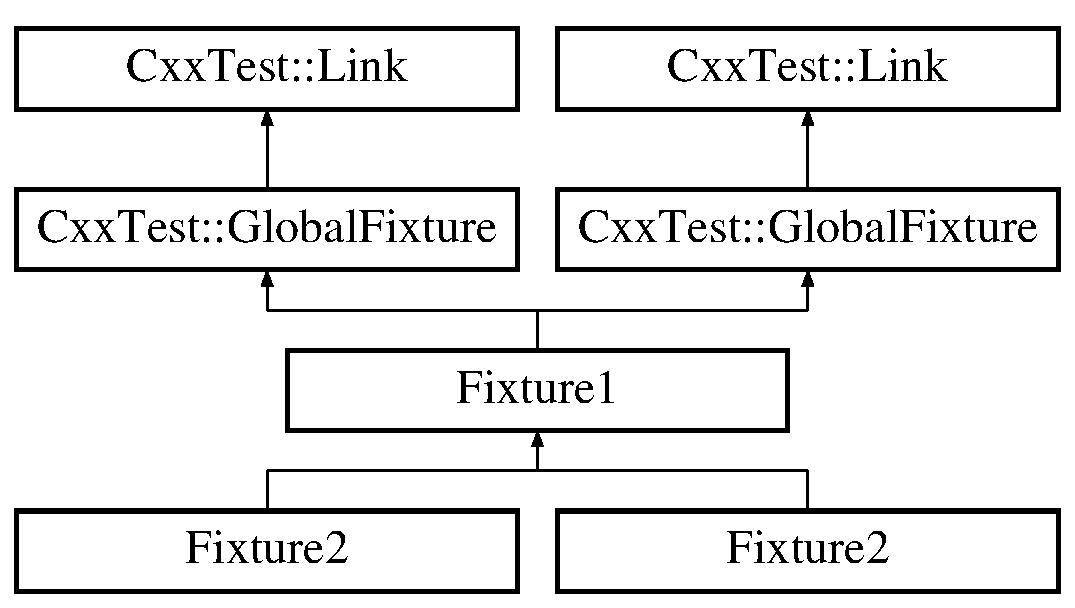
\includegraphics[height=4.000000cm]{classFixture1}
\end{center}
\end{figure}
\subsection*{Public Member Functions}
\begin{DoxyCompactItemize}
\item 
\hypertarget{classFixture1_add920b52688f1d7dcd0cc707d8c20975}{bool {\bfseries set\-Up} ()}\label{classFixture1_add920b52688f1d7dcd0cc707d8c20975}

\item 
\hypertarget{classFixture1_a9eb75c966931827abd4ae37ca7b83208}{bool {\bfseries tear\-Down} ()}\label{classFixture1_a9eb75c966931827abd4ae37ca7b83208}

\item 
\hypertarget{classFixture1_ae287a60f3709a69699744c7fb3abedeb}{bool {\bfseries set\-Up\-World} ()}\label{classFixture1_ae287a60f3709a69699744c7fb3abedeb}

\item 
\hypertarget{classFixture1_a02aaa8adfed0aa20e4e46c97ddbfa467}{bool {\bfseries tear\-Down\-World} ()}\label{classFixture1_a02aaa8adfed0aa20e4e46c97ddbfa467}

\item 
\hypertarget{classFixture1_add920b52688f1d7dcd0cc707d8c20975}{bool {\bfseries set\-Up} ()}\label{classFixture1_add920b52688f1d7dcd0cc707d8c20975}

\item 
\hypertarget{classFixture1_a9eb75c966931827abd4ae37ca7b83208}{bool {\bfseries tear\-Down} ()}\label{classFixture1_a9eb75c966931827abd4ae37ca7b83208}

\item 
\hypertarget{classFixture1_ac46fd4df91b45f32c2d5cbb3e805ed08}{unsigned {\bfseries set\-Up\-Count} () const }\label{classFixture1_ac46fd4df91b45f32c2d5cbb3e805ed08}

\item 
\hypertarget{classFixture1_a2290f361acd0c3ffe40c8a7faca501c0}{unsigned {\bfseries tear\-Down\-Count} () const }\label{classFixture1_a2290f361acd0c3ffe40c8a7faca501c0}

\end{DoxyCompactItemize}
\subsection*{Public Attributes}
\begin{DoxyCompactItemize}
\item 
\hypertarget{classFixture1_a96bbcbb9676f40f19d903615ec18ce2c}{unsigned {\bfseries set\-Up\-Count}}\label{classFixture1_a96bbcbb9676f40f19d903615ec18ce2c}

\item 
\hypertarget{classFixture1_a0df398d82b296ff27e787346d5e05830}{unsigned {\bfseries tear\-Down\-Count}}\label{classFixture1_a0df398d82b296ff27e787346d5e05830}

\end{DoxyCompactItemize}
\subsection*{Additional Inherited Members}


The documentation for this class was generated from the following files\-:\begin{DoxyCompactItemize}
\item 
test/cxxtest/doc/examples/My\-Test\-Suite8.\-h\item 
test/cxxtest/test/Global\-Fixtures.\-h\end{DoxyCompactItemize}

\hypertarget{classFixture2}{\section{Fixture2 Class Reference}
\label{classFixture2}\index{Fixture2@{Fixture2}}
}
Inheritance diagram for Fixture2\-:\begin{figure}[H]
\begin{center}
\leavevmode
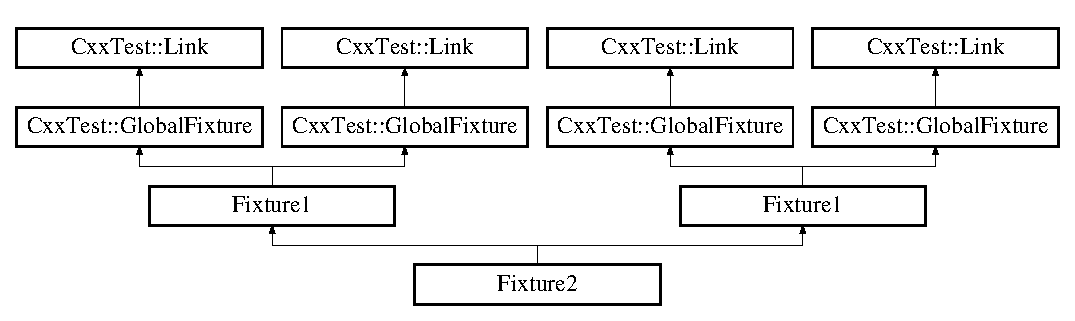
\includegraphics[height=3.862069cm]{classFixture2}
\end{center}
\end{figure}
\subsection*{Public Member Functions}
\begin{DoxyCompactItemize}
\item 
\hypertarget{classFixture2_a7e49022158ef6fde84e8de248ccb376e}{bool {\bfseries set\-Up} ()}\label{classFixture2_a7e49022158ef6fde84e8de248ccb376e}

\item 
\hypertarget{classFixture2_ad3ba6f79ab507f3aa2d0832e72bbe461}{bool {\bfseries tear\-Down} ()}\label{classFixture2_ad3ba6f79ab507f3aa2d0832e72bbe461}

\item 
\hypertarget{classFixture2_a7e49022158ef6fde84e8de248ccb376e}{bool {\bfseries set\-Up} ()}\label{classFixture2_a7e49022158ef6fde84e8de248ccb376e}

\item 
\hypertarget{classFixture2_ad3ba6f79ab507f3aa2d0832e72bbe461}{bool {\bfseries tear\-Down} ()}\label{classFixture2_ad3ba6f79ab507f3aa2d0832e72bbe461}

\end{DoxyCompactItemize}
\subsection*{Additional Inherited Members}


The documentation for this class was generated from the following files\-:\begin{DoxyCompactItemize}
\item 
test/cxxtest/doc/examples/My\-Test\-Suite8.\-h\item 
test/cxxtest/test/Global\-Fixtures.\-h\end{DoxyCompactItemize}

\hypertarget{classFixtureTest}{\section{Fixture\-Test Class Reference}
\label{classFixtureTest}\index{Fixture\-Test@{Fixture\-Test}}
}
Inheritance diagram for Fixture\-Test\-:\begin{figure}[H]
\begin{center}
\leavevmode
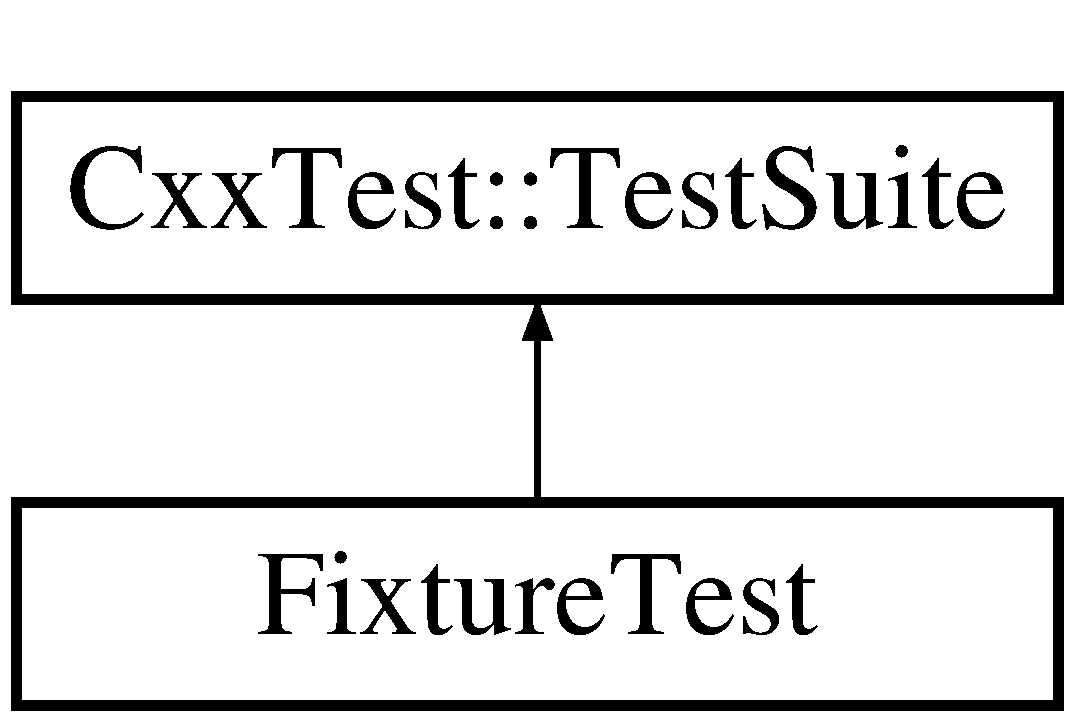
\includegraphics[height=2.000000cm]{classFixtureTest}
\end{center}
\end{figure}
\subsection*{Public Member Functions}
\begin{DoxyCompactItemize}
\item 
\hypertarget{classFixtureTest_a9ae41eaed04c146917655810eb98f81f}{void {\bfseries set\-Up} ()}\label{classFixtureTest_a9ae41eaed04c146917655810eb98f81f}

\item 
\hypertarget{classFixtureTest_acd647e2ed9c294ae5d6d986bd583dcce}{void {\bfseries tear\-Down} ()}\label{classFixtureTest_acd647e2ed9c294ae5d6d986bd583dcce}

\item 
\hypertarget{classFixtureTest_adaeddbf61bb1e8de4c8c29d9846cc710}{void {\bfseries test\-\_\-strcpy} ()}\label{classFixtureTest_adaeddbf61bb1e8de4c8c29d9846cc710}

\end{DoxyCompactItemize}


The documentation for this class was generated from the following file\-:\begin{DoxyCompactItemize}
\item 
test/cxxtest/sample/Fixture\-Test.\-h\end{DoxyCompactItemize}

\hypertarget{classFlashPhotoApp}{\section{Flash\-Photo\-App Class Reference}
\label{classFlashPhotoApp}\index{Flash\-Photo\-App@{Flash\-Photo\-App}}
}
Inheritance diagram for Flash\-Photo\-App\-:\begin{figure}[H]
\begin{center}
\leavevmode
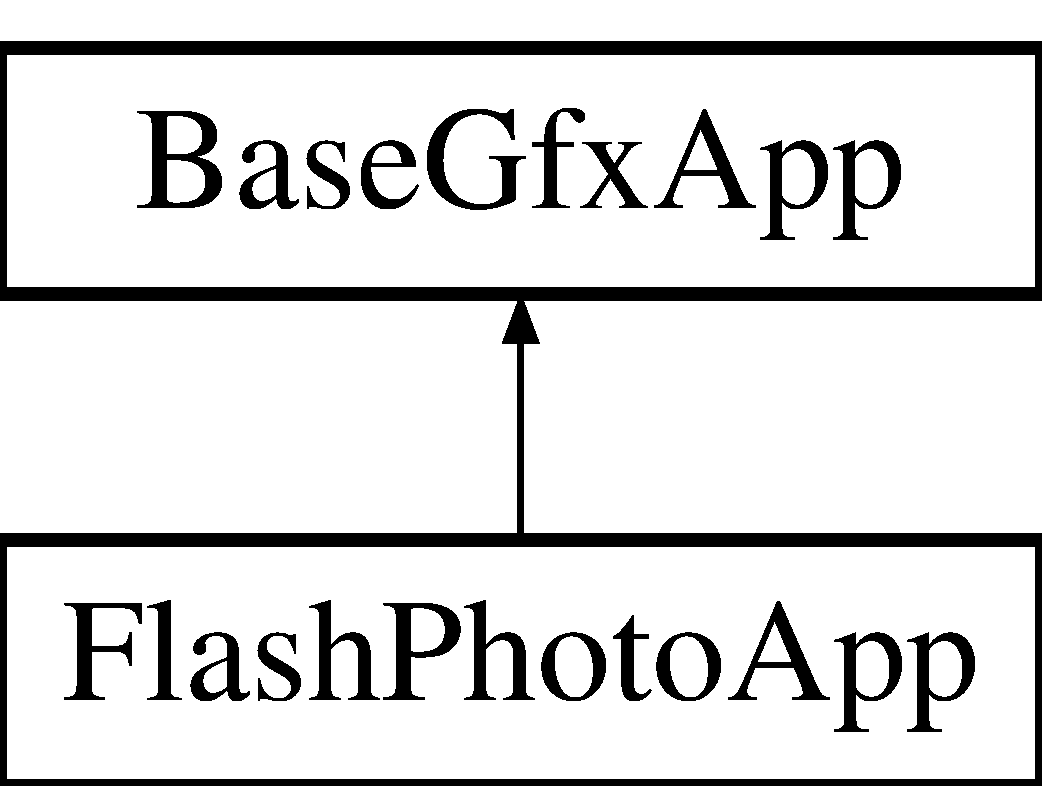
\includegraphics[height=2.000000cm]{classFlashPhotoApp}
\end{center}
\end{figure}
\subsection*{Public Member Functions}
\begin{DoxyCompactItemize}
\item 
\hyperlink{classFlashPhotoApp_a944931218613603cfb6bda6113971382}{Flash\-Photo\-App} (int argc, char $\ast$argv\mbox{[}$\,$\mbox{]}, int width, int height, \hyperlink{classColorData}{Color\-Data} background\-Color)
\item 
\hypertarget{classFlashPhotoApp_a29505b498fac898e099cfd1b8590c91a}{void \hyperlink{classFlashPhotoApp_a29505b498fac898e099cfd1b8590c91a}{mouse\-Dragged} (int x, int y)}\label{classFlashPhotoApp_a29505b498fac898e099cfd1b8590c91a}

\begin{DoxyCompactList}\small\item\em When the mouse is dragged this function is called. \end{DoxyCompactList}\item 
\hypertarget{classFlashPhotoApp_acf5a4cc5b76bb676d337758543bfdcc4}{void \hyperlink{classFlashPhotoApp_acf5a4cc5b76bb676d337758543bfdcc4}{mouse\-Moved} (int x, int y)}\label{classFlashPhotoApp_acf5a4cc5b76bb676d337758543bfdcc4}

\begin{DoxyCompactList}\small\item\em When the mouse if moved this function is called. \end{DoxyCompactList}\item 
\hypertarget{classFlashPhotoApp_a2c348ddcc15b6a21972bc6aac98c5442}{void \hyperlink{classFlashPhotoApp_a2c348ddcc15b6a21972bc6aac98c5442}{left\-Mouse\-Down} (int x, int y)}\label{classFlashPhotoApp_a2c348ddcc15b6a21972bc6aac98c5442}

\begin{DoxyCompactList}\small\item\em When the left mouse button is pressed this function is called. \end{DoxyCompactList}\item 
\hypertarget{classFlashPhotoApp_ae3a2f37b7c3657dcb5c16402c6d25519}{void \hyperlink{classFlashPhotoApp_ae3a2f37b7c3657dcb5c16402c6d25519}{left\-Mouse\-Up} (int x, int y)}\label{classFlashPhotoApp_ae3a2f37b7c3657dcb5c16402c6d25519}

\begin{DoxyCompactList}\small\item\em When the left mouse button is let go this function is called. \end{DoxyCompactList}\item 
\hypertarget{classFlashPhotoApp_a5dedc84bbc9ea0cf0718b8d0d0f414a5}{void {\bfseries display} ()}\label{classFlashPhotoApp_a5dedc84bbc9ea0cf0718b8d0d0f414a5}

\item 
\hypertarget{classFlashPhotoApp_aaeea3b8490d0f0239e41b781f6a066aa}{void {\bfseries glui\-Control} (int control\-I\-D)}\label{classFlashPhotoApp_aaeea3b8490d0f0239e41b781f6a066aa}

\end{DoxyCompactItemize}
\subsection*{Private Types}
\begin{DoxyCompactItemize}
\item 
enum {\bfseries U\-I\-Control\-Type} \{ \\*
{\bfseries U\-I\-\_\-\-T\-O\-O\-L\-T\-Y\-P\-E}, 
{\bfseries U\-I\-\_\-\-C\-O\-L\-O\-R\-\_\-\-R}, 
{\bfseries U\-I\-\_\-\-C\-O\-L\-O\-R\-\_\-\-G}, 
{\bfseries U\-I\-\_\-\-C\-O\-L\-O\-R\-\_\-\-B}, 
\\*
{\bfseries U\-I\-\_\-\-P\-R\-E\-S\-E\-T\-\_\-\-R\-E\-D}, 
{\bfseries U\-I\-\_\-\-P\-R\-E\-S\-E\-T\-\_\-\-O\-R\-A\-N\-G\-E}, 
{\bfseries U\-I\-\_\-\-P\-R\-E\-S\-E\-T\-\_\-\-Y\-E\-L\-L\-O\-W}, 
{\bfseries U\-I\-\_\-\-P\-R\-E\-S\-E\-T\-\_\-\-G\-R\-E\-E\-N}, 
\\*
{\bfseries U\-I\-\_\-\-P\-R\-E\-S\-E\-T\-\_\-\-B\-L\-U\-E}, 
{\bfseries U\-I\-\_\-\-P\-R\-E\-S\-E\-T\-\_\-\-P\-U\-R\-P\-L\-E}, 
{\bfseries U\-I\-\_\-\-P\-R\-E\-S\-E\-T\-\_\-\-W\-H\-I\-T\-E}, 
{\bfseries U\-I\-\_\-\-P\-R\-E\-S\-E\-T\-\_\-\-B\-L\-A\-C\-K}, 
\\*
{\bfseries U\-I\-\_\-\-F\-I\-L\-E\-\_\-\-B\-R\-O\-W\-S\-E\-R}, 
{\bfseries U\-I\-\_\-\-L\-O\-A\-D\-\_\-\-C\-A\-N\-V\-A\-S\-\_\-\-B\-U\-T\-T\-O\-N}, 
{\bfseries U\-I\-\_\-\-L\-O\-A\-D\-\_\-\-S\-T\-A\-M\-P\-\_\-\-B\-U\-T\-T\-O\-N}, 
{\bfseries U\-I\-\_\-\-S\-A\-V\-E\-\_\-\-C\-A\-N\-V\-A\-S\-\_\-\-B\-U\-T\-T\-O\-N}, 
\\*
{\bfseries U\-I\-\_\-\-F\-I\-L\-E\-\_\-\-N\-A\-M\-E}, 
{\bfseries U\-I\-\_\-\-A\-P\-P\-L\-Y\-\_\-\-B\-L\-U\-R}, 
{\bfseries U\-I\-\_\-\-A\-P\-P\-L\-Y\-\_\-\-S\-H\-A\-R\-P}, 
{\bfseries U\-I\-\_\-\-A\-P\-P\-L\-Y\-\_\-\-E\-D\-G\-E}, 
\\*
{\bfseries U\-I\-\_\-\-A\-P\-P\-L\-Y\-\_\-\-T\-H\-R\-E\-S\-H\-O\-L\-D}, 
{\bfseries U\-I\-\_\-\-A\-P\-P\-L\-Y\-\_\-\-D\-I\-T\-H\-E\-R}, 
{\bfseries U\-I\-\_\-\-A\-P\-P\-L\-Y\-\_\-\-S\-A\-T\-U\-R\-A\-T\-E}, 
{\bfseries U\-I\-\_\-\-A\-P\-P\-L\-Y\-\_\-\-C\-H\-A\-N\-N\-E\-L}, 
\\*
{\bfseries U\-I\-\_\-\-A\-P\-P\-L\-Y\-\_\-\-Q\-U\-A\-N\-T\-I\-Z\-E}, 
{\bfseries U\-I\-\_\-\-A\-P\-P\-L\-Y\-\_\-\-M\-O\-T\-I\-O\-N\-\_\-\-B\-L\-U\-R}, 
{\bfseries U\-I\-\_\-\-A\-P\-P\-L\-Y\-\_\-\-S\-P\-E\-C\-I\-A\-L\-\_\-\-F\-I\-L\-T\-E\-R}, 
{\bfseries U\-I\-\_\-\-U\-N\-D\-O}, 
\\*
{\bfseries U\-I\-\_\-\-R\-E\-D\-O}, 
{\bfseries U\-I\-\_\-\-C\-L\-E\-A\-R}, 
{\bfseries U\-I\-\_\-\-Q\-U\-I\-T}
 \}
\item 
enum {\bfseries U\-I\-Motion\-Blur\-Directions} \{ {\bfseries D\-I\-R\-\_\-\-N\-\_\-\-S}, 
{\bfseries D\-I\-R\-\_\-\-E\-\_\-\-W}, 
{\bfseries D\-I\-R\-\_\-\-N\-E\-\_\-\-S\-W}, 
{\bfseries D\-I\-R\-\_\-\-N\-W\-\_\-\-S\-E}
 \}
\item 
enum {\bfseries Tool\-Type} \{ \\*
{\bfseries P\-E\-N}, 
{\bfseries E\-R\-A\-S\-E\-R}, 
{\bfseries S\-P\-R\-A\-Y\-C\-A\-N}, 
{\bfseries C\-A\-L\-I\-G\-R\-A\-P\-H\-Y\-P\-E\-N}, 
\\*
{\bfseries H\-I\-G\-H\-L\-I\-G\-H\-T\-E\-R}, 
{\bfseries W\-A\-T\-E\-R\-C\-O\-L\-O\-R}, 
{\bfseries F\-I\-L\-L\-T\-O\-O\-L}, 
{\bfseries C\-R\-A\-Y\-O\-N}, 
\\*
{\bfseries S\-T\-A\-M\-P}, 
{\bfseries B\-L\-U\-R}
 \}
\end{DoxyCompactItemize}
\subsection*{Private Member Functions}
\begin{DoxyCompactItemize}
\item 
\hypertarget{classFlashPhotoApp_a262d3fad41e5feb441b4ea431c65f8c1}{void {\bfseries set\-Image\-File} (const std\-::string \&filepath)}\label{classFlashPhotoApp_a262d3fad41e5feb441b4ea431c65f8c1}

\item 
\hypertarget{classFlashPhotoApp_a05fb136c74949eb11f07f161e18b0e44}{bool {\bfseries is\-Valid\-Image\-File\-Name} (const std\-::string \&name)}\label{classFlashPhotoApp_a05fb136c74949eb11f07f161e18b0e44}

\item 
\hypertarget{classFlashPhotoApp_af9f413e89445c3a0210e69d542affd67}{bool {\bfseries is\-Valid\-Image\-File} (const std\-::string \&name)}\label{classFlashPhotoApp_af9f413e89445c3a0210e69d542affd67}

\item 
\hypertarget{classFlashPhotoApp_a346a7760598d8dd3c6ddb0630b1e51b6}{bool {\bfseries has\-Suffix} (const std\-::string \&str, const std\-::string \&suffix)}\label{classFlashPhotoApp_a346a7760598d8dd3c6ddb0630b1e51b6}

\item 
\hypertarget{classFlashPhotoApp_a886a76eaa5e30c1708a96cc62cd98887}{void {\bfseries button\-Enabled} (G\-L\-U\-I\-\_\-\-Button $\ast$button, bool enabled)}\label{classFlashPhotoApp_a886a76eaa5e30c1708a96cc62cd98887}

\item 
\hypertarget{classFlashPhotoApp_aa4ceaa973c4cd8b953e4e09d0a5a81ff}{void {\bfseries undo\-Enabled} (bool enabled)}\label{classFlashPhotoApp_aa4ceaa973c4cd8b953e4e09d0a5a81ff}

\item 
\hypertarget{classFlashPhotoApp_a03e224580f502076a6c498a35fb8069f}{void {\bfseries redo\-Enabled} (bool enabled)}\label{classFlashPhotoApp_a03e224580f502076a6c498a35fb8069f}

\item 
\hypertarget{classFlashPhotoApp_af370462c4a82dd932ae7364fc58e3959}{void {\bfseries save\-Canvas\-Enabled} (bool enabled)}\label{classFlashPhotoApp_af370462c4a82dd932ae7364fc58e3959}

\item 
\hypertarget{classFlashPhotoApp_aa04f2738fdb07a7eaa86f146c7537a70}{void {\bfseries load\-Canvas\-Enabled} (bool enabled)}\label{classFlashPhotoApp_aa04f2738fdb07a7eaa86f146c7537a70}

\item 
\hypertarget{classFlashPhotoApp_a9e58a2c36d94fcbe376f3cb5b75ad5e0}{void {\bfseries load\-Stamp\-Enabled} (bool enabled)}\label{classFlashPhotoApp_a9e58a2c36d94fcbe376f3cb5b75ad5e0}

\item 
\hypertarget{classFlashPhotoApp_ad554624b8359abe270e5c6e76634ff48}{void {\bfseries update\-Colors} ()}\label{classFlashPhotoApp_ad554624b8359abe270e5c6e76634ff48}

\item 
void \hyperlink{classFlashPhotoApp_a29383606562f09ba623209581f92f5e5}{init\-Draw\-Tool} ()
\item 
void \hyperlink{classFlashPhotoApp_aeaf85d6ead6ca4b3905701db12ceaf68}{init\-Filter} ()
\item 
void \hyperlink{classFlashPhotoApp_a52eb2524a928df150d75492d96a3d49c}{update\-Current\-Tool} ()
\item 
void \hyperlink{classFlashPhotoApp_a7cc9f1383c18cb7eebc255d3c377adb0}{load\-Image\-To\-Canvas} ()
\item 
\hypertarget{classFlashPhotoApp_a87aee2ef5baef954b682c67e3d5118da}{void {\bfseries load\-Image\-To\-Stamp} ()}\label{classFlashPhotoApp_a87aee2ef5baef954b682c67e3d5118da}

\item 
void \hyperlink{classFlashPhotoApp_ab0389fb3c2c64e0e3312880e745b7070}{save\-Canvas\-To\-File} ()
\item 
\hypertarget{classFlashPhotoApp_a16ff3baa9c0d97d8e4f292acb4ebbfac}{void {\bfseries apply\-Filter\-Blur} ()}\label{classFlashPhotoApp_a16ff3baa9c0d97d8e4f292acb4ebbfac}

\item 
\hypertarget{classFlashPhotoApp_a9d45a9f24245024cba2c9090d7acb528}{void {\bfseries apply\-Filter\-Sharpen} ()}\label{classFlashPhotoApp_a9d45a9f24245024cba2c9090d7acb528}

\item 
\hypertarget{classFlashPhotoApp_af99c135d287d07e01ccd1637cba0d347}{void {\bfseries apply\-Filter\-Motion\-Blur} ()}\label{classFlashPhotoApp_af99c135d287d07e01ccd1637cba0d347}

\item 
\hypertarget{classFlashPhotoApp_ae7360d5fc26c2789d0126defb1c30e9f}{void {\bfseries apply\-Filter\-Edge\-Detect} ()}\label{classFlashPhotoApp_ae7360d5fc26c2789d0126defb1c30e9f}

\item 
\hypertarget{classFlashPhotoApp_a316479ee5fc48b785c266953147de63e}{void {\bfseries apply\-Filter\-Threshold} ()}\label{classFlashPhotoApp_a316479ee5fc48b785c266953147de63e}

\item 
\hypertarget{classFlashPhotoApp_a8c8d8c714d059083f49e1e0cd1336321}{void {\bfseries apply\-Filter\-Channel} ()}\label{classFlashPhotoApp_a8c8d8c714d059083f49e1e0cd1336321}

\item 
\hypertarget{classFlashPhotoApp_aabd2e2b487ebe038cbcbfa700d5951f9}{void {\bfseries apply\-Filter\-Saturate} ()}\label{classFlashPhotoApp_aabd2e2b487ebe038cbcbfa700d5951f9}

\item 
\hypertarget{classFlashPhotoApp_a5a9c62db1aa83250b4f95c94f5dac762}{void {\bfseries apply\-Filter\-Quantize} ()}\label{classFlashPhotoApp_a5a9c62db1aa83250b4f95c94f5dac762}

\item 
\hypertarget{classFlashPhotoApp_a7b1664e842e4a0a16cf7c340e126de17}{void {\bfseries apply\-Filter\-Special} ()}\label{classFlashPhotoApp_a7b1664e842e4a0a16cf7c340e126de17}

\item 
\hypertarget{classFlashPhotoApp_ad33153aceb1cca61bb682c00ae8e22ff}{void {\bfseries undo\-Operation} ()}\label{classFlashPhotoApp_ad33153aceb1cca61bb682c00ae8e22ff}

\item 
\hypertarget{classFlashPhotoApp_aad1a00932e723e17c39f6959c42d9f5f}{void {\bfseries redo\-Operation} ()}\label{classFlashPhotoApp_aad1a00932e723e17c39f6959c42d9f5f}

\item 
void \hyperlink{classFlashPhotoApp_af90d307fdc027a037816a63757a17120}{update\-Canvas} (std\-::deque$<$ \hyperlink{classPixelBuffer}{Pixel\-Buffer} $\ast$ $>$ \&alpha, std\-::deque$<$ \hyperlink{classPixelBuffer}{Pixel\-Buffer} $\ast$ $>$ \&beta, bool is\-Undo)
\item 
\hypertarget{classFlashPhotoApp_a8360b752328c423d850d819361e18a12}{void {\bfseries init\-Glui} ()}\label{classFlashPhotoApp_a8360b752328c423d850d819361e18a12}

\item 
\hypertarget{classFlashPhotoApp_a9a786ee86c70c142fd957421f9354996}{void {\bfseries init\-Graphics} ()}\label{classFlashPhotoApp_a9a786ee86c70c142fd957421f9354996}

\item 
\hypertarget{classFlashPhotoApp_afed06134c0c49494fb5055a93dc8423f}{void {\bfseries initialize\-Buffers} (\hyperlink{classColorData}{Color\-Data} initial\-Color, int width, int height)}\label{classFlashPhotoApp_afed06134c0c49494fb5055a93dc8423f}

\item 
\hypertarget{classFlashPhotoApp_a2dc3dd9da509fb67ab5ae61b6a8d9c03}{bool {\bfseries isjpeg} (const std\-::string \&name)}\label{classFlashPhotoApp_a2dc3dd9da509fb67ab5ae61b6a8d9c03}

\item 
\hypertarget{classFlashPhotoApp_aa53b230edec12feb0ed4e5531cdd760e}{int {\bfseries loadpng} (F\-I\-L\-E $\ast$fp)}\label{classFlashPhotoApp_aa53b230edec12feb0ed4e5531cdd760e}

\item 
void \hyperlink{classFlashPhotoApp_a7dc31c434067d59fa14d40e22a21d66c}{clear\-Pixel\-Buffer} ()
\item 
\hypertarget{classFlashPhotoApp_ae578c10b12f1f39d52d2fe2e4f0f5b96}{void {\bfseries update\-Undo} ()}\label{classFlashPhotoApp_ae578c10b12f1f39d52d2fe2e4f0f5b96}

\end{DoxyCompactItemize}
\subsection*{Private Attributes}
\begin{DoxyCompactItemize}
\item 
\hypertarget{classFlashPhotoApp_adc1082b61b8e0650f8dba72e0ac9c90d}{\begin{tabbing}
xx\=xx\=xx\=xx\=xx\=xx\=xx\=xx\=xx\=\kill
struct \{\\
\hypertarget{structFlashPhotoApp_1_1@0_a24bac49f0d04130b0012f82c7683afac}{\>float {\bfseries channel\_colorRed}\\
\hypertarget{structFlashPhotoApp_1_1@0_ac18742e7fcb8534d9476c100d742358d}{\>float {\bfseries channel\_colorGreen}\\
\hypertarget{structFlashPhotoApp_1_1@0_aaad046817775345700256c63ee69a066}{\>float {\bfseries channel\_colorBlue}\\
\hypertarget{structFlashPhotoApp_1_1@0_a507851bce4f4af02c093a1d28a088da7}{\>float {\bfseries saturation\_amount}\\
\hypertarget{structFlashPhotoApp_1_1@0_a47e02008d3de690cd60c97df03e4d8fd}{\>float {\bfseries threshold\_amount}\\
\hypertarget{structFlashPhotoApp_1_1@0_abe620dc3be32a15e2a87426eae4b9429}{\>float {\bfseries blur\_amount}\\
\hypertarget{structFlashPhotoApp_1_1@0_ab8ddc9587fc24a36c5eb1ddf1380ef99}{\>float {\bfseries sharpen\_amount}\\
\hypertarget{structFlashPhotoApp_1_1@0_a224bd3b1ac652128da1736dbd855a467}{\>float {\bfseries motionBlur\_amount}\\
\hypertarget{structFlashPhotoApp_1_1@0_a37732ed053efaac3198792777abc537a}{\>int {\bfseries motionBlur\_direction}\\
\hypertarget{structFlashPhotoApp_1_1@0_a21466a62d5a49b29052541c1bdaaff82}{\>int {\bfseries quantize\_bins}\\
\} {\bfseries m\_filterParameters}}\label{classFlashPhotoApp_adc1082b61b8e0650f8dba72e0ac9c90d}
\\

\end{tabbing}\item 
\hypertarget{classFlashPhotoApp_a26ed03c8eea24f9b2193fe98f02a78b7}{\begin{tabbing}
xx\=xx\=xx\=xx\=xx\=xx\=xx\=xx\=xx\=\kill
struct \{\\
\hypertarget{structFlashPhotoApp_1_1@1_a6e190905f22d88f7155b5e4fea7e82e2}{\>GLUI\_FileBrowser $\ast$ {\bfseries fileBrowser}\\
\hypertarget{structFlashPhotoApp_1_1@1_a568203b21cda88b7f64a5339064a7d18}{\>GLUI\_Button $\ast$ {\bfseries loadCanvasButton}\\
\hypertarget{structFlashPhotoApp_1_1@1_aa4aa83844dfbaac5e2601d9ecf252e60}{\>GLUI\_Button $\ast$ {\bfseries loadStampButton}\\
\hypertarget{structFlashPhotoApp_1_1@1_a1b1c7930ccf25d66161aa0bd0926f885}{\>GLUI\_Button $\ast$ {\bfseries saveCanvasButton}\\
\hypertarget{structFlashPhotoApp_1_1@1_a96d62cf788203344f8941b79170fc346}{\>GLUI\_Button $\ast$ {\bfseries redoButton}\\
\hypertarget{structFlashPhotoApp_1_1@1_abce09e914786f07c8de6e675574e7681}{\>GLUI\_Button $\ast$ {\bfseries undoButton}\\
\hypertarget{structFlashPhotoApp_1_1@1_af6bf7b007ec57149ac322bb039b36448}{\>GLUI\_StaticText $\ast$ {\bfseries currentFileLabel}\\
\hypertarget{structFlashPhotoApp_1_1@1_abe3d1fbda64a09063e4d3a5f33c1d860}{\>GLUI\_EditText $\ast$ {\bfseries fileNameBox}\\
\hypertarget{structFlashPhotoApp_1_1@1_a830a100998dba74fbb5c71566ae20460}{\>GLUI\_StaticText $\ast$ {\bfseries saveFileLabel}\\
\hypertarget{structFlashPhotoApp_1_1@1_a54d8c8487ee6d847b9dc38f3f03f78db}{\>GLUI\_Spinner $\ast$ {\bfseries spinnerRed}\\
\hypertarget{structFlashPhotoApp_1_1@1_ac912473a2801aa9bfe9fcf1072e48627}{\>GLUI\_Spinner $\ast$ {\bfseries spinnerGreen}\\
\hypertarget{structFlashPhotoApp_1_1@1_acc6dc220ee767f7b5b113e26ddbc18b9}{\>GLUI\_Spinner $\ast$ {\bfseries spinnerBlue}\\
\} {\bfseries m\_gluiControlHooks}}\label{classFlashPhotoApp_a26ed03c8eea24f9b2193fe98f02a78b7}
\\

\end{tabbing}\item 
\hypertarget{classFlashPhotoApp_ae45bc3761686cbb4d5f9c01b048816c0}{int {\bfseries m\-\_\-queue\-Size}}\label{classFlashPhotoApp_ae45bc3761686cbb4d5f9c01b048816c0}

\item 
\hypertarget{classFlashPhotoApp_abdb0f4d46432039c14d5816abb019fa7}{std\-::deque$<$ \hyperlink{classPixelBuffer}{Pixel\-Buffer} $\ast$ $>$ {\bfseries undo\-Queue}}\label{classFlashPhotoApp_abdb0f4d46432039c14d5816abb019fa7}

\item 
\hypertarget{classFlashPhotoApp_a67142e2e575f5c63666b3e750279fd4f}{std\-::deque$<$ \hyperlink{classPixelBuffer}{Pixel\-Buffer} $\ast$ $>$ {\bfseries redo\-Queue}}\label{classFlashPhotoApp_a67142e2e575f5c63666b3e750279fd4f}

\item 
\hypertarget{classFlashPhotoApp_a7552f6cf6441c53d020e5a0124031bcb}{int {\bfseries m\-\_\-prev\-X}}\label{classFlashPhotoApp_a7552f6cf6441c53d020e5a0124031bcb}

\item 
\hypertarget{classFlashPhotoApp_a6a9759bdfbdf16bf0091f1694604a64a}{int {\bfseries m\-\_\-prev\-Y}}\label{classFlashPhotoApp_a6a9759bdfbdf16bf0091f1694604a64a}

\item 
\hypertarget{classFlashPhotoApp_a2e397b37bfb3ea981efc795b7a2a9e9e}{int {\bfseries m\-\_\-stamp\-Height}}\label{classFlashPhotoApp_a2e397b37bfb3ea981efc795b7a2a9e9e}

\item 
\hypertarget{classFlashPhotoApp_a7dab8bf3eb60e4c99310660c9c32f3a5}{int {\bfseries m\-\_\-stamp\-Width}}\label{classFlashPhotoApp_a7dab8bf3eb60e4c99310660c9c32f3a5}

\item 
\hypertarget{classFlashPhotoApp_a9662e1dbd6e003a62179eecba827e910}{\hyperlink{classPixelBuffer}{Pixel\-Buffer} $\ast$ {\bfseries m\-\_\-display\-Buffer}}\label{classFlashPhotoApp_a9662e1dbd6e003a62179eecba827e910}

\item 
\hypertarget{classFlashPhotoApp_a752ba29ca132a3fd4deaa3727946f7f6}{\hyperlink{classDrawTool}{Draw\-Tool} $\ast$$\ast$ {\bfseries tool\-List}}\label{classFlashPhotoApp_a752ba29ca132a3fd4deaa3727946f7f6}

\item 
\hypertarget{classFlashPhotoApp_a69d8dcf7147882964a6d2832bbab67e2}{\hyperlink{classDrawTool}{Draw\-Tool} $\ast$ {\bfseries m\-\_\-tool}}\label{classFlashPhotoApp_a69d8dcf7147882964a6d2832bbab67e2}

\item 
\hypertarget{classFlashPhotoApp_a4fe8a885ae7b5e698c40a7585b4e292d}{int {\bfseries m\-\_\-cur\-Tool}}\label{classFlashPhotoApp_a4fe8a885ae7b5e698c40a7585b4e292d}

\item 
\hypertarget{classFlashPhotoApp_a40ef9e2d21c3f80cee59be363e21b9bc}{\hyperlink{classFilter}{Filter} $\ast$$\ast$ {\bfseries m\-\_\-filters}}\label{classFlashPhotoApp_a40ef9e2d21c3f80cee59be363e21b9bc}

\item 
\hypertarget{classFlashPhotoApp_a584dd16d8f2aad51028759a1dd94c83f}{int {\bfseries m\-\_\-cur\-Filter}}\label{classFlashPhotoApp_a584dd16d8f2aad51028759a1dd94c83f}

\item 
\hypertarget{classFlashPhotoApp_a6e4b0ca13b038233f14563c79f7201ae}{float {\bfseries m\-\_\-cur\-Color\-Red}}\label{classFlashPhotoApp_a6e4b0ca13b038233f14563c79f7201ae}

\item 
\hypertarget{classFlashPhotoApp_a3af18066365495dda69e11a3b5116ee6}{float {\bfseries m\-\_\-cur\-Color\-Green}}\label{classFlashPhotoApp_a3af18066365495dda69e11a3b5116ee6}

\item 
\hypertarget{classFlashPhotoApp_a1c7b40fbfe40343ff9653120b6925f09}{float {\bfseries m\-\_\-cur\-Color\-Blue}}\label{classFlashPhotoApp_a1c7b40fbfe40343ff9653120b6925f09}

\item 
\hypertarget{classFlashPhotoApp_a110a669df9d98f66a68b9d2eec6a9748}{std\-::string {\bfseries m\-\_\-file\-Name}}\label{classFlashPhotoApp_a110a669df9d98f66a68b9d2eec6a9748}

\end{DoxyCompactItemize}
\subsection*{Additional Inherited Members}


\subsection{Constructor \& Destructor Documentation}
\hypertarget{classFlashPhotoApp_a944931218613603cfb6bda6113971382}{\index{Flash\-Photo\-App@{Flash\-Photo\-App}!Flash\-Photo\-App@{Flash\-Photo\-App}}
\index{Flash\-Photo\-App@{Flash\-Photo\-App}!FlashPhotoApp@{Flash\-Photo\-App}}
\subsubsection[{Flash\-Photo\-App}]{\setlength{\rightskip}{0pt plus 5cm}Flash\-Photo\-App\-::\-Flash\-Photo\-App (
\begin{DoxyParamCaption}
\item[{int}]{argc, }
\item[{char $\ast$}]{argv\mbox{[}$\,$\mbox{]}, }
\item[{int}]{width, }
\item[{int}]{height, }
\item[{{\bf Color\-Data}}]{background\-Color}
\end{DoxyParamCaption}
)}}\label{classFlashPhotoApp_a944931218613603cfb6bda6113971382}
This is the Flash\-Photo class. This class contains all of the main U\-I login for the application. 

\subsection{Member Function Documentation}
\hypertarget{classFlashPhotoApp_a7dc31c434067d59fa14d40e22a21d66c}{\index{Flash\-Photo\-App@{Flash\-Photo\-App}!clear\-Pixel\-Buffer@{clear\-Pixel\-Buffer}}
\index{clear\-Pixel\-Buffer@{clear\-Pixel\-Buffer}!FlashPhotoApp@{Flash\-Photo\-App}}
\subsubsection[{clear\-Pixel\-Buffer}]{\setlength{\rightskip}{0pt plus 5cm}void Flash\-Photo\-App\-::clear\-Pixel\-Buffer (
\begin{DoxyParamCaption}
{}
\end{DoxyParamCaption}
)\hspace{0.3cm}{\ttfamily [private]}}}\label{classFlashPhotoApp_a7dc31c434067d59fa14d40e22a21d66c}
Clear the pixel buffer back to the default buffer color \par
none \par
void \par
\hypertarget{classFlashPhotoApp_a29383606562f09ba623209581f92f5e5}{\index{Flash\-Photo\-App@{Flash\-Photo\-App}!init\-Draw\-Tool@{init\-Draw\-Tool}}
\index{init\-Draw\-Tool@{init\-Draw\-Tool}!FlashPhotoApp@{Flash\-Photo\-App}}
\subsubsection[{init\-Draw\-Tool}]{\setlength{\rightskip}{0pt plus 5cm}void Flash\-Photo\-App\-::init\-Draw\-Tool (
\begin{DoxyParamCaption}
{}
\end{DoxyParamCaption}
)\hspace{0.3cm}{\ttfamily [private]}}}\label{classFlashPhotoApp_a29383606562f09ba623209581f92f5e5}
Initialize the draw tool on load \par
none \par
void \par
\hypertarget{classFlashPhotoApp_aeaf85d6ead6ca4b3905701db12ceaf68}{\index{Flash\-Photo\-App@{Flash\-Photo\-App}!init\-Filter@{init\-Filter}}
\index{init\-Filter@{init\-Filter}!FlashPhotoApp@{Flash\-Photo\-App}}
\subsubsection[{init\-Filter}]{\setlength{\rightskip}{0pt plus 5cm}void Flash\-Photo\-App\-::init\-Filter (
\begin{DoxyParamCaption}
{}
\end{DoxyParamCaption}
)\hspace{0.3cm}{\ttfamily [private]}}}\label{classFlashPhotoApp_aeaf85d6ead6ca4b3905701db12ceaf68}
Initialize the filter on load \par
none \par
void \par
\hypertarget{classFlashPhotoApp_a7cc9f1383c18cb7eebc255d3c377adb0}{\index{Flash\-Photo\-App@{Flash\-Photo\-App}!load\-Image\-To\-Canvas@{load\-Image\-To\-Canvas}}
\index{load\-Image\-To\-Canvas@{load\-Image\-To\-Canvas}!FlashPhotoApp@{Flash\-Photo\-App}}
\subsubsection[{load\-Image\-To\-Canvas}]{\setlength{\rightskip}{0pt plus 5cm}void Flash\-Photo\-App\-::load\-Image\-To\-Canvas (
\begin{DoxyParamCaption}
{}
\end{DoxyParamCaption}
)\hspace{0.3cm}{\ttfamily [private]}}}\label{classFlashPhotoApp_a7cc9f1383c18cb7eebc255d3c377adb0}
Load an image on to the canvas \par
none \par
void \par
\hypertarget{classFlashPhotoApp_ab0389fb3c2c64e0e3312880e745b7070}{\index{Flash\-Photo\-App@{Flash\-Photo\-App}!save\-Canvas\-To\-File@{save\-Canvas\-To\-File}}
\index{save\-Canvas\-To\-File@{save\-Canvas\-To\-File}!FlashPhotoApp@{Flash\-Photo\-App}}
\subsubsection[{save\-Canvas\-To\-File}]{\setlength{\rightskip}{0pt plus 5cm}void Flash\-Photo\-App\-::save\-Canvas\-To\-File (
\begin{DoxyParamCaption}
{}
\end{DoxyParamCaption}
)\hspace{0.3cm}{\ttfamily [private]}}}\label{classFlashPhotoApp_ab0389fb3c2c64e0e3312880e745b7070}
Save a canvas to file \par
none \par
void \par
\hypertarget{classFlashPhotoApp_af90d307fdc027a037816a63757a17120}{\index{Flash\-Photo\-App@{Flash\-Photo\-App}!update\-Canvas@{update\-Canvas}}
\index{update\-Canvas@{update\-Canvas}!FlashPhotoApp@{Flash\-Photo\-App}}
\subsubsection[{update\-Canvas}]{\setlength{\rightskip}{0pt plus 5cm}void Flash\-Photo\-App\-::update\-Canvas (
\begin{DoxyParamCaption}
\item[{std\-::deque$<$ {\bf Pixel\-Buffer} $\ast$ $>$ \&}]{alpha, }
\item[{std\-::deque$<$ {\bf Pixel\-Buffer} $\ast$ $>$ \&}]{beta, }
\item[{bool}]{is\-Undo}
\end{DoxyParamCaption}
)\hspace{0.3cm}{\ttfamily [private]}}}\label{classFlashPhotoApp_af90d307fdc027a037816a63757a17120}
Update the canvas with the top of the alpha deque, push current buffer onto beta deque \par
deque to pop from, deque to push to, if it is an undo \par
void \par
\hypertarget{classFlashPhotoApp_a52eb2524a928df150d75492d96a3d49c}{\index{Flash\-Photo\-App@{Flash\-Photo\-App}!update\-Current\-Tool@{update\-Current\-Tool}}
\index{update\-Current\-Tool@{update\-Current\-Tool}!FlashPhotoApp@{Flash\-Photo\-App}}
\subsubsection[{update\-Current\-Tool}]{\setlength{\rightskip}{0pt plus 5cm}void Flash\-Photo\-App\-::update\-Current\-Tool (
\begin{DoxyParamCaption}
{}
\end{DoxyParamCaption}
)\hspace{0.3cm}{\ttfamily [private]}}}\label{classFlashPhotoApp_a52eb2524a928df150d75492d96a3d49c}
Update the current tool that is selected in the U\-I (stored in m\-\_\-cur\-Tool) \par
none \par
void \par


The documentation for this class was generated from the following files\-:\begin{DoxyCompactItemize}
\item 
Flash\-Photo/Flash\-Photo\-App.\-h\item 
Flash\-Photo/Flash\-Photo\-App.\-cpp\end{DoxyCompactItemize}

\hypertarget{classFMotionBlur}{\section{F\-Motion\-Blur Class Reference}
\label{classFMotionBlur}\index{F\-Motion\-Blur@{F\-Motion\-Blur}}
}
Inheritance diagram for F\-Motion\-Blur\-:\begin{figure}[H]
\begin{center}
\leavevmode
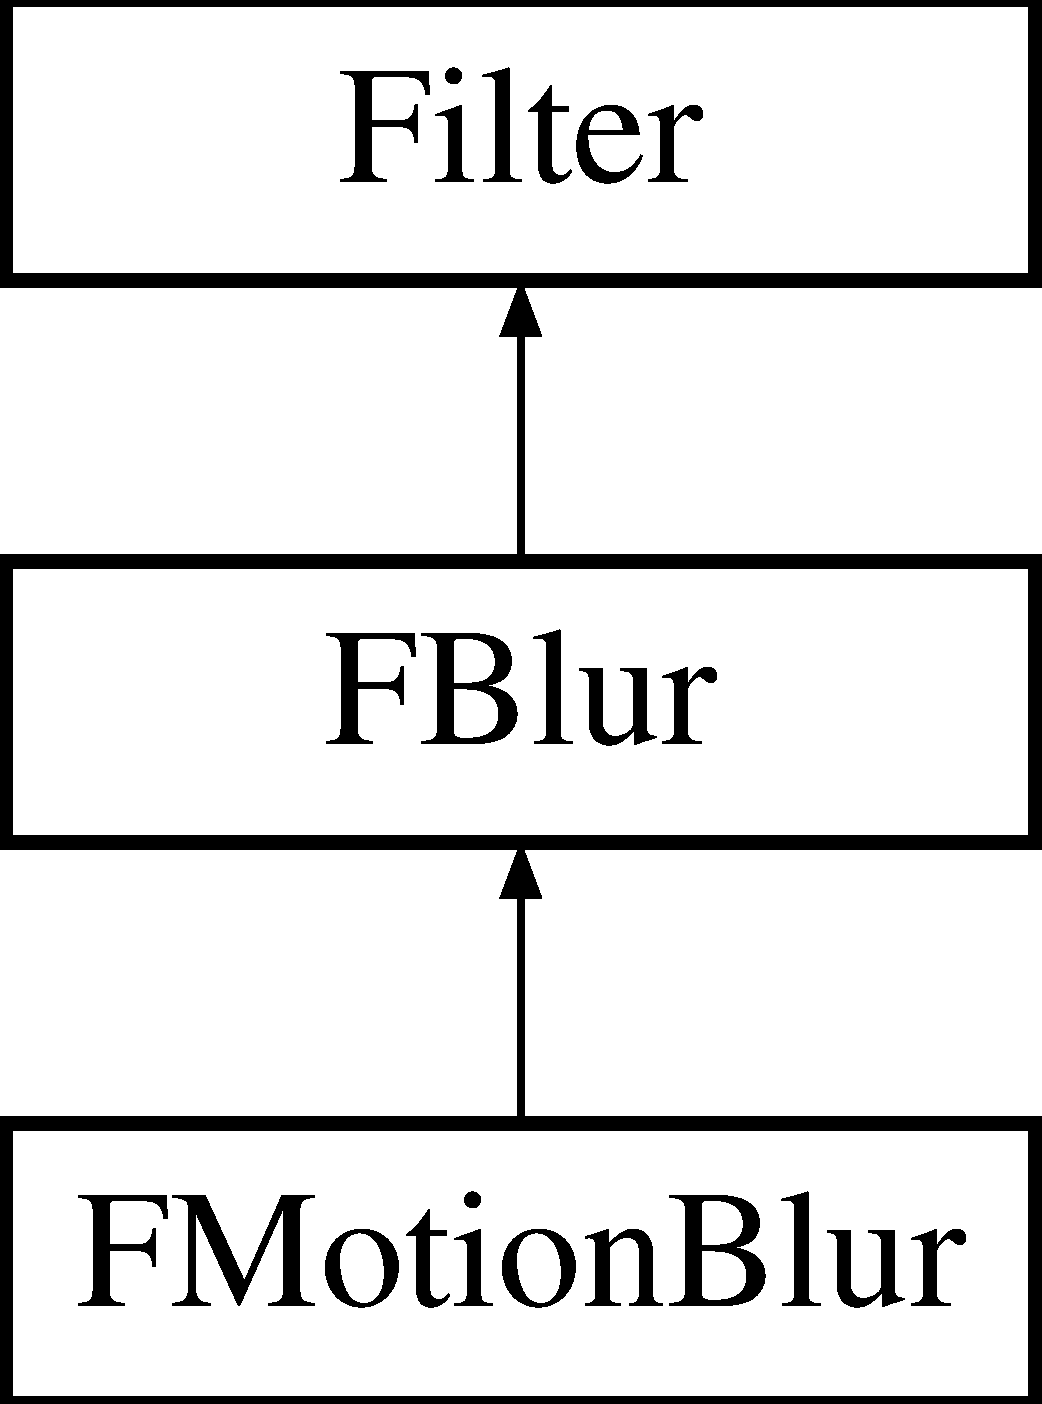
\includegraphics[height=3.000000cm]{classFMotionBlur}
\end{center}
\end{figure}
\subsection*{Public Types}
\begin{DoxyCompactItemize}
\item 
enum {\bfseries Motion\-Blur\-Directions} \{ {\bfseries D\-I\-R\-\_\-\-N\-\_\-\-S}, 
{\bfseries D\-I\-R\-\_\-\-E\-\_\-\-W}, 
{\bfseries D\-I\-R\-\_\-\-N\-E\-\_\-\-S\-W}, 
{\bfseries D\-I\-R\-\_\-\-N\-W\-\_\-\-S\-E}
 \}
\end{DoxyCompactItemize}
\subsection*{Public Member Functions}
\begin{DoxyCompactItemize}
\item 
\hyperlink{classFMotionBlur_a670df8e9b43ff1ff3b262b6d48b944cf}{F\-Motion\-Blur} ()
\item 
\hypertarget{classFMotionBlur_aeb40f52478dcf27d5fa8fec4aa473975}{std\-::string {\bfseries get\-Name} ()}\label{classFMotionBlur_aeb40f52478dcf27d5fa8fec4aa473975}

\item 
\hypertarget{classFMotionBlur_a105abc618c4fe5ddd890ad2ff1836979}{kernel\-Type {\bfseries build\-Kernel} (int radius)}\label{classFMotionBlur_a105abc618c4fe5ddd890ad2ff1836979}

\end{DoxyCompactItemize}


\subsection{Constructor \& Destructor Documentation}
\hypertarget{classFMotionBlur_a670df8e9b43ff1ff3b262b6d48b944cf}{\index{F\-Motion\-Blur@{F\-Motion\-Blur}!F\-Motion\-Blur@{F\-Motion\-Blur}}
\index{F\-Motion\-Blur@{F\-Motion\-Blur}!FMotionBlur@{F\-Motion\-Blur}}
\subsubsection[{F\-Motion\-Blur}]{\setlength{\rightskip}{0pt plus 5cm}F\-Motion\-Blur\-::\-F\-Motion\-Blur (
\begin{DoxyParamCaption}
{}
\end{DoxyParamCaption}
)}}\label{classFMotionBlur_a670df8e9b43ff1ff3b262b6d48b944cf}
This is the F\-Motion class, it is used for the motion blur image filters. It inherits from the \hyperlink{classFBlur}{F\-Blur} class, so it only needs to build\-Kernel, not apply it. 

The documentation for this class was generated from the following files\-:\begin{DoxyCompactItemize}
\item 
libphoto/F\-Motion\-Blur.\-h\item 
libphoto/F\-Motion\-Blur.\-cpp\end{DoxyCompactItemize}

\hypertarget{classFooTestSuite1}{\section{Foo\-Test\-Suite1 Class Reference}
\label{classFooTestSuite1}\index{Foo\-Test\-Suite1@{Foo\-Test\-Suite1}}
}
Inheritance diagram for Foo\-Test\-Suite1\-:\begin{figure}[H]
\begin{center}
\leavevmode
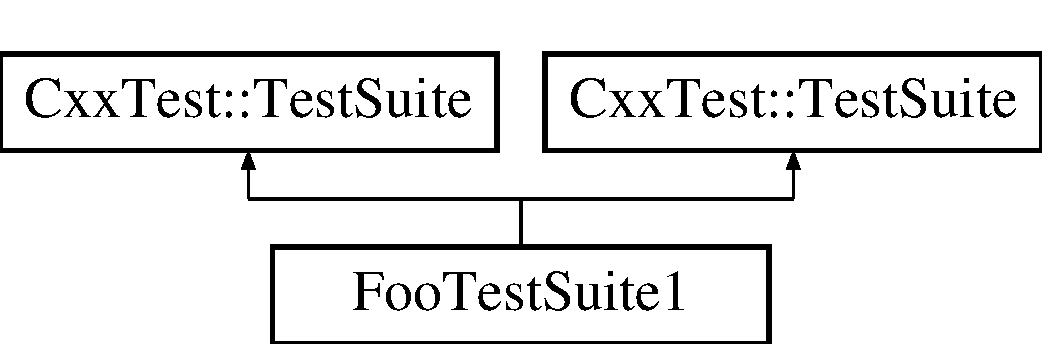
\includegraphics[height=2.000000cm]{classFooTestSuite1}
\end{center}
\end{figure}
\subsection*{Public Member Functions}
\begin{DoxyCompactItemize}
\item 
\hypertarget{classFooTestSuite1_af2a11d94d9c19582dcf0258557c70efc}{void {\bfseries test\-Foo} (void)}\label{classFooTestSuite1_af2a11d94d9c19582dcf0258557c70efc}

\item 
\hypertarget{classFooTestSuite1_af2a11d94d9c19582dcf0258557c70efc}{void {\bfseries test\-Foo} (void)}\label{classFooTestSuite1_af2a11d94d9c19582dcf0258557c70efc}

\end{DoxyCompactItemize}


The documentation for this class was generated from the following files\-:\begin{DoxyCompactItemize}
\item 
test/cxxtest/build\-\_\-tools/\-S\-Cons/test/libpath/test/test.\-t.\-h\item 
test/cxxtest/build\-\_\-tools/\-S\-Cons/test/libpath\-\_\-multitarget/test/test1.\-t.\-h\end{DoxyCompactItemize}

\hypertarget{classForceNoEh}{\section{Force\-No\-Eh Class Reference}
\label{classForceNoEh}\index{Force\-No\-Eh@{Force\-No\-Eh}}
}
Inheritance diagram for Force\-No\-Eh\-:\begin{figure}[H]
\begin{center}
\leavevmode
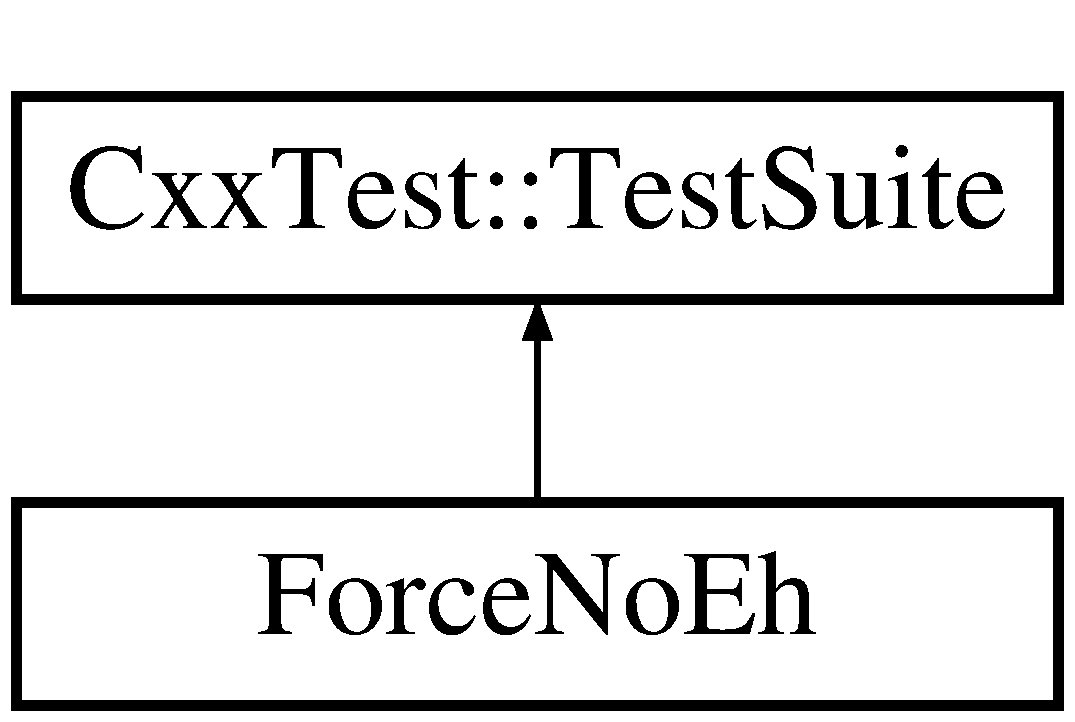
\includegraphics[height=2.000000cm]{classForceNoEh}
\end{center}
\end{figure}
\subsection*{Public Member Functions}
\begin{DoxyCompactItemize}
\item 
\hypertarget{classForceNoEh_abe967f9e39eba1c8674517e9efd3c1de}{void {\bfseries test\-Cxx\-Test\-Can\-Compile\-Without\-Exception\-Handling} ()}\label{classForceNoEh_abe967f9e39eba1c8674517e9efd3c1de}

\item 
\hypertarget{classForceNoEh_a8f62139e5d1d3c74253c73c727a2d921}{void {\bfseries foo} ()}\label{classForceNoEh_a8f62139e5d1d3c74253c73c727a2d921}

\end{DoxyCompactItemize}


The documentation for this class was generated from the following file\-:\begin{DoxyCompactItemize}
\item 
test/cxxtest/test/Force\-No\-Eh.\-h\end{DoxyCompactItemize}

\hypertarget{classFQuantize}{\section{F\-Quantize Class Reference}
\label{classFQuantize}\index{F\-Quantize@{F\-Quantize}}
}
Inheritance diagram for F\-Quantize\-:\begin{figure}[H]
\begin{center}
\leavevmode
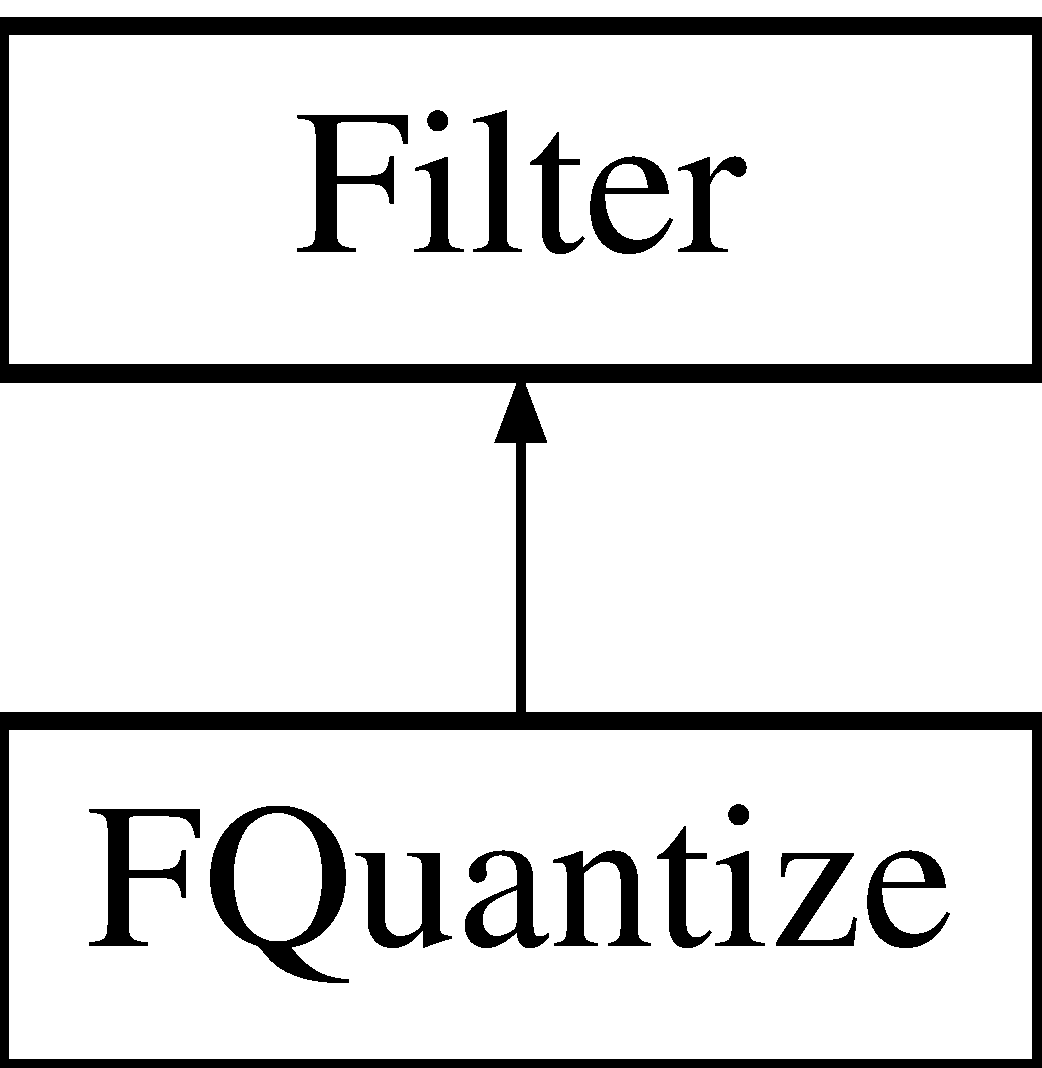
\includegraphics[height=2.000000cm]{classFQuantize}
\end{center}
\end{figure}
\subsection*{Public Member Functions}
\begin{DoxyCompactItemize}
\item 
\hypertarget{classFQuantize_a093d0f34480882da50d994eb4e450c64}{void {\bfseries apply\-Filter} (\hyperlink{classPixelBuffer}{Pixel\-Buffer} $\ast$image\-Buffer)}\label{classFQuantize_a093d0f34480882da50d994eb4e450c64}

\item 
\hypertarget{classFQuantize_a9432e52568e0b7608522569e0a438a1d}{std\-::string {\bfseries get\-Name} ()}\label{classFQuantize_a9432e52568e0b7608522569e0a438a1d}

\item 
\hypertarget{classFQuantize_a093d0f34480882da50d994eb4e450c64}{void {\bfseries apply\-Filter} (\hyperlink{classPixelBuffer}{Pixel\-Buffer} $\ast$image\-Buffer)}\label{classFQuantize_a093d0f34480882da50d994eb4e450c64}

\item 
\hypertarget{classFQuantize_a9432e52568e0b7608522569e0a438a1d}{std\-::string {\bfseries get\-Name} ()}\label{classFQuantize_a9432e52568e0b7608522569e0a438a1d}

\item 
\hypertarget{classFQuantize_a093d0f34480882da50d994eb4e450c64}{void {\bfseries apply\-Filter} (\hyperlink{classPixelBuffer}{Pixel\-Buffer} $\ast$image\-Buffer)}\label{classFQuantize_a093d0f34480882da50d994eb4e450c64}

\item 
\hypertarget{classFQuantize_a9432e52568e0b7608522569e0a438a1d}{std\-::string {\bfseries get\-Name} ()}\label{classFQuantize_a9432e52568e0b7608522569e0a438a1d}

\end{DoxyCompactItemize}


The documentation for this class was generated from the following files\-:\begin{DoxyCompactItemize}
\item 
libphoto/F\-Quantize.\-h\item 
libphoto/include/libphoto.\-h\item 
libphoto/F\-Quantize.\-cpp\end{DoxyCompactItemize}

\hypertarget{classFSaturation}{}\section{F\+Saturation Class Reference}
\label{classFSaturation}\index{F\+Saturation@{F\+Saturation}}
Inheritance diagram for F\+Saturation\+:\begin{figure}[H]
\begin{center}
\leavevmode
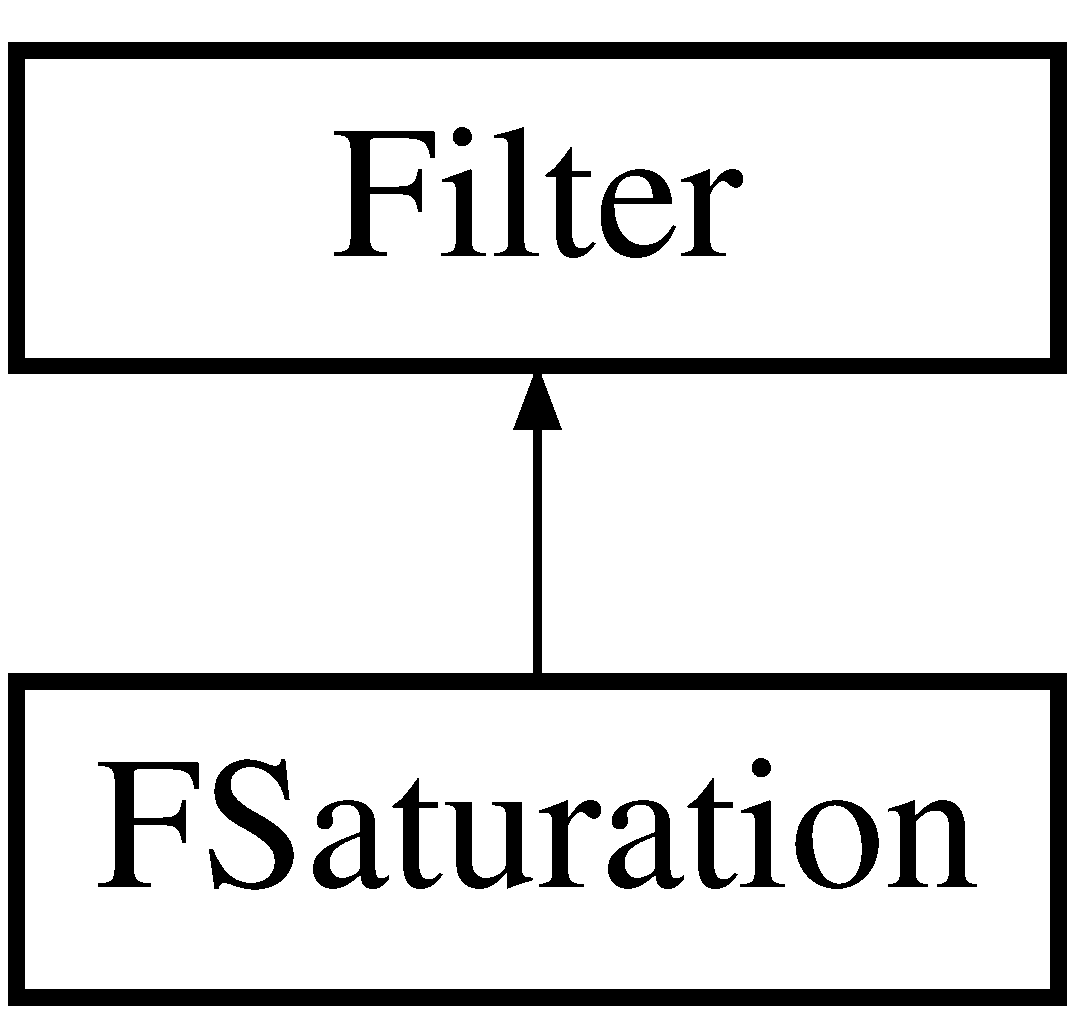
\includegraphics[height=2.000000cm]{classFSaturation}
\end{center}
\end{figure}
\subsection*{Public Member Functions}
\begin{DoxyCompactItemize}
\item 
\hyperlink{classFSaturation_a164678727eb7204e4946578b339617b7}{F\+Saturation} ()
\item 
void \hyperlink{classFSaturation_a9e35fd05500411807bfcbe36b8f24a55}{apply\+Filter} (\hyperlink{classPixelBuffer}{Pixel\+Buffer} $\ast$image\+Buffer)\hypertarget{classFSaturation_a9e35fd05500411807bfcbe36b8f24a55}{}\label{classFSaturation_a9e35fd05500411807bfcbe36b8f24a55}

\begin{DoxyCompactList}\small\item\em apply filter effect to Pixel\+Buffer$\ast$ buffer passed into this function \end{DoxyCompactList}\item 
std\+::string \hyperlink{classFSaturation_a55d272a3a50fcb65d94a66821b7b0c73}{get\+Name} ()\hypertarget{classFSaturation_a55d272a3a50fcb65d94a66821b7b0c73}{}\label{classFSaturation_a55d272a3a50fcb65d94a66821b7b0c73}

\begin{DoxyCompactList}\small\item\em get class name for filter \end{DoxyCompactList}\end{DoxyCompactItemize}


\subsection{Constructor \& Destructor Documentation}
\index{F\+Saturation@{F\+Saturation}!F\+Saturation@{F\+Saturation}}
\index{F\+Saturation@{F\+Saturation}!F\+Saturation@{F\+Saturation}}
\subsubsection[{\texorpdfstring{F\+Saturation()}{FSaturation()}}]{\setlength{\rightskip}{0pt plus 5cm}F\+Saturation\+::\+F\+Saturation (
\begin{DoxyParamCaption}
{}
\end{DoxyParamCaption}
)}\hypertarget{classFSaturation_a164678727eb7204e4946578b339617b7}{}\label{classFSaturation_a164678727eb7204e4946578b339617b7}
This is the \hyperlink{classFSaturation}{F\+Saturation} class, it is used for the saturation image filters. This does not use kernels so it only has to deal with applying the filter 

The documentation for this class was generated from the following files\+:\begin{DoxyCompactItemize}
\item 
libphoto/F\+Saturation.\+h\item 
libphoto/F\+Saturation.\+cpp\end{DoxyCompactItemize}

\hypertarget{classFSharpen}{\section{F\-Sharpen Class Reference}
\label{classFSharpen}\index{F\-Sharpen@{F\-Sharpen}}
}
Inheritance diagram for F\-Sharpen\-:\begin{figure}[H]
\begin{center}
\leavevmode
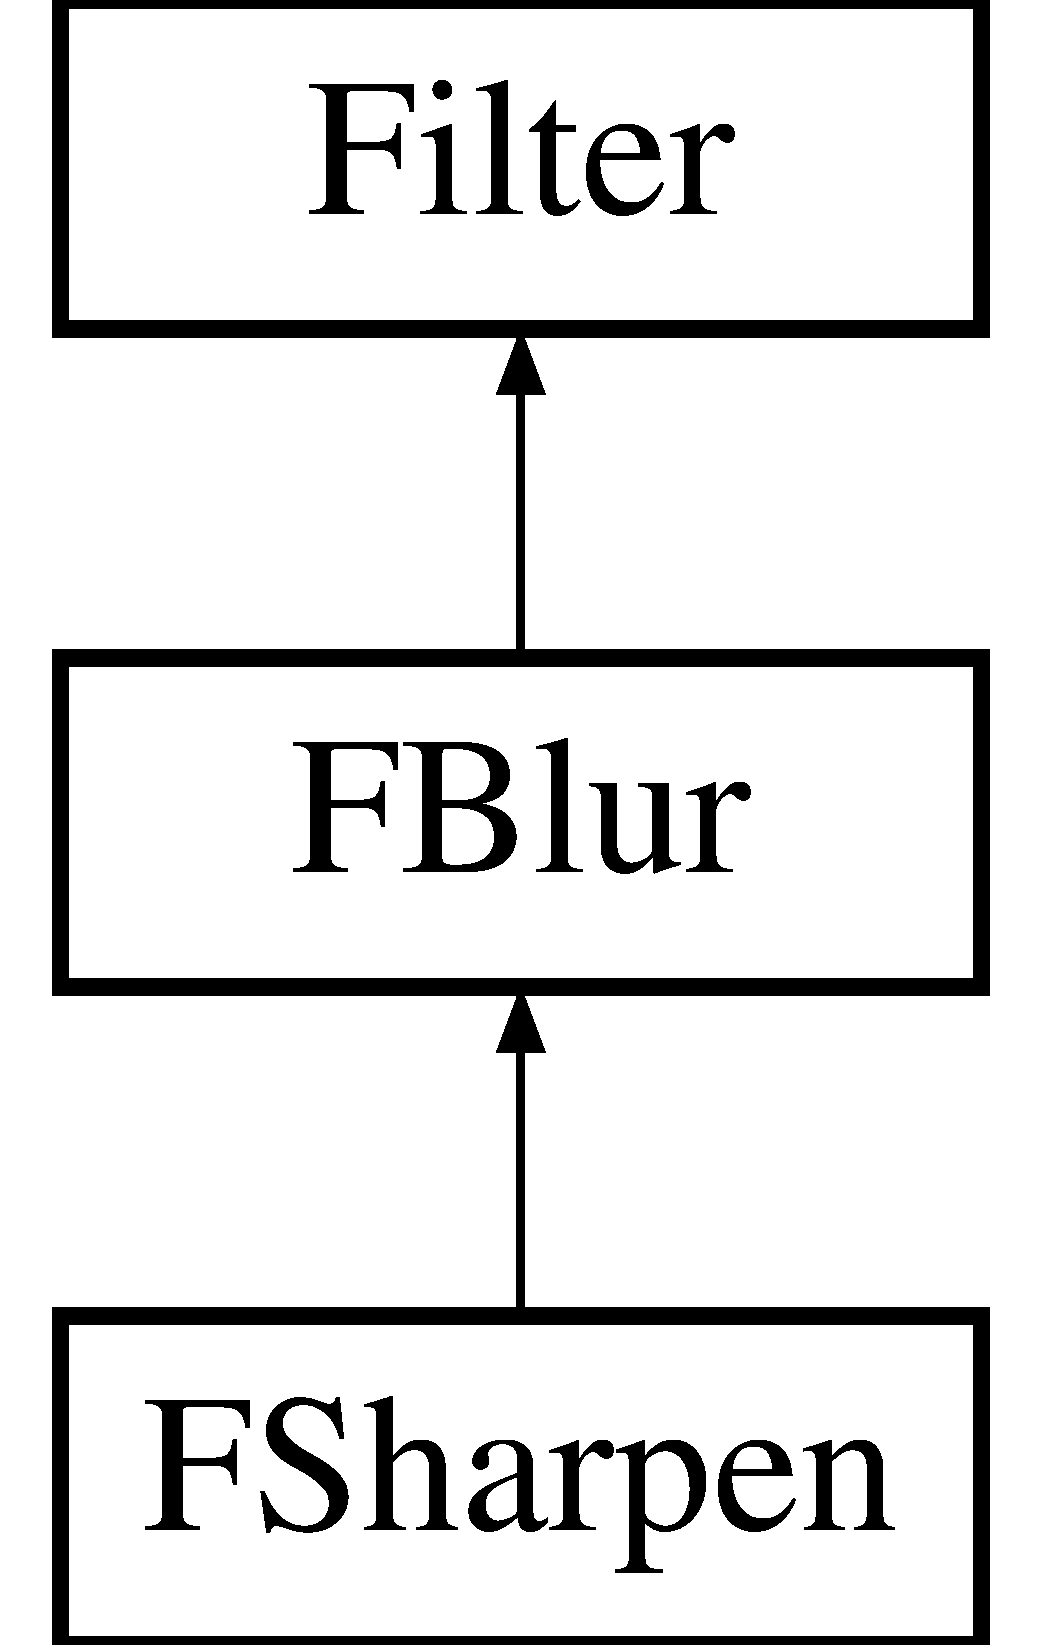
\includegraphics[height=3.000000cm]{classFSharpen}
\end{center}
\end{figure}
\subsection*{Public Member Functions}
\begin{DoxyCompactItemize}
\item 
\hypertarget{classFSharpen_ae322ad5626a003ae1e1c6e385dd43ca8}{std\-::string {\bfseries get\-Name} ()}\label{classFSharpen_ae322ad5626a003ae1e1c6e385dd43ca8}

\item 
\hypertarget{classFSharpen_afafd2b34e58d2fb682150be2159d7986}{kernel\-Type {\bfseries build\-Kernel} (int radius)}\label{classFSharpen_afafd2b34e58d2fb682150be2159d7986}

\end{DoxyCompactItemize}


The documentation for this class was generated from the following files\-:\begin{DoxyCompactItemize}
\item 
libphoto/F\-Sharpen.\-h\item 
libphoto/F\-Sharpen.\-cpp\end{DoxyCompactItemize}

\hypertarget{classFSpecial}{\section{F\-Special Class Reference}
\label{classFSpecial}\index{F\-Special@{F\-Special}}
}
Inheritance diagram for F\-Special\-:\begin{figure}[H]
\begin{center}
\leavevmode
\includegraphics[height=2.000000cm]{classFSpecial}
\end{center}
\end{figure}
\subsection*{Public Member Functions}
\begin{DoxyCompactItemize}
\item 
\hypertarget{classFSpecial_ad5af4242e35da376aeb628e6a7cabc5e}{void {\bfseries apply\-Filter} (\hyperlink{classPixelBuffer}{Pixel\-Buffer} $\ast$image\-Buffer)}\label{classFSpecial_ad5af4242e35da376aeb628e6a7cabc5e}

\item 
\hypertarget{classFSpecial_a769159ff4dc9f6ebd64a6bbe5ae2e917}{std\-::string {\bfseries get\-Name} ()}\label{classFSpecial_a769159ff4dc9f6ebd64a6bbe5ae2e917}

\item 
\hypertarget{classFSpecial_ad5af4242e35da376aeb628e6a7cabc5e}{void {\bfseries apply\-Filter} (\hyperlink{classPixelBuffer}{Pixel\-Buffer} $\ast$image\-Buffer)}\label{classFSpecial_ad5af4242e35da376aeb628e6a7cabc5e}

\item 
\hypertarget{classFSpecial_a769159ff4dc9f6ebd64a6bbe5ae2e917}{std\-::string {\bfseries get\-Name} ()}\label{classFSpecial_a769159ff4dc9f6ebd64a6bbe5ae2e917}

\item 
\hypertarget{classFSpecial_ad5af4242e35da376aeb628e6a7cabc5e}{void {\bfseries apply\-Filter} (\hyperlink{classPixelBuffer}{Pixel\-Buffer} $\ast$image\-Buffer)}\label{classFSpecial_ad5af4242e35da376aeb628e6a7cabc5e}

\item 
\hypertarget{classFSpecial_a769159ff4dc9f6ebd64a6bbe5ae2e917}{std\-::string {\bfseries get\-Name} ()}\label{classFSpecial_a769159ff4dc9f6ebd64a6bbe5ae2e917}

\end{DoxyCompactItemize}


The documentation for this class was generated from the following files\-:\begin{DoxyCompactItemize}
\item 
libphoto/F\-Special.\-h\item 
libphoto/include/libphoto.\-h\item 
libphoto/F\-Special.\-cpp\end{DoxyCompactItemize}

\hypertarget{classFThreshold}{\section{F\-Threshold Class Reference}
\label{classFThreshold}\index{F\-Threshold@{F\-Threshold}}
}
Inheritance diagram for F\-Threshold\-:\begin{figure}[H]
\begin{center}
\leavevmode
\includegraphics[height=2.000000cm]{classFThreshold}
\end{center}
\end{figure}
\subsection*{Public Member Functions}
\begin{DoxyCompactItemize}
\item 
\hypertarget{classFThreshold_a324dadf15c23bd2d2edf6ea32e3d87f6}{void {\bfseries apply\-Filter} (\hyperlink{classPixelBuffer}{Pixel\-Buffer} $\ast$image\-Buffer)}\label{classFThreshold_a324dadf15c23bd2d2edf6ea32e3d87f6}

\item 
\hypertarget{classFThreshold_a189f8f15c0719706a7eb191b198c0b15}{std\-::string {\bfseries get\-Name} ()}\label{classFThreshold_a189f8f15c0719706a7eb191b198c0b15}

\end{DoxyCompactItemize}


The documentation for this class was generated from the following files\-:\begin{DoxyCompactItemize}
\item 
libphoto/F\-Threshold.\-h\item 
libphoto/F\-Threshold.\-cpp\end{DoxyCompactItemize}

\hypertarget{classCxxTest_1_1GlobalFixture}{\section{Cxx\-Test\-:\-:Global\-Fixture Class Reference}
\label{classCxxTest_1_1GlobalFixture}\index{Cxx\-Test\-::\-Global\-Fixture@{Cxx\-Test\-::\-Global\-Fixture}}
}
Inheritance diagram for Cxx\-Test\-:\-:Global\-Fixture\-:\begin{figure}[H]
\begin{center}
\leavevmode
\includegraphics[height=12.000000cm]{classCxxTest_1_1GlobalFixture}
\end{center}
\end{figure}
\subsection*{Public Member Functions}
\begin{DoxyCompactItemize}
\item 
\hypertarget{classCxxTest_1_1GlobalFixture_a38d38d51f0bf725262bdc52915a2c7ab}{virtual bool {\bfseries set\-Up\-World} ()}\label{classCxxTest_1_1GlobalFixture_a38d38d51f0bf725262bdc52915a2c7ab}

\item 
\hypertarget{classCxxTest_1_1GlobalFixture_afefd57ebe829308b138d40580e8f935d}{virtual bool {\bfseries tear\-Down\-World} ()}\label{classCxxTest_1_1GlobalFixture_afefd57ebe829308b138d40580e8f935d}

\item 
\hypertarget{classCxxTest_1_1GlobalFixture_a5edcee94174c4452e6a3d4cd6c190b74}{virtual bool {\bfseries set\-Up} ()}\label{classCxxTest_1_1GlobalFixture_a5edcee94174c4452e6a3d4cd6c190b74}

\item 
\hypertarget{classCxxTest_1_1GlobalFixture_a0d79953ba5fb3f0ec5bf2e6d2fa0a1d1}{virtual bool {\bfseries tear\-Down} ()}\label{classCxxTest_1_1GlobalFixture_a0d79953ba5fb3f0ec5bf2e6d2fa0a1d1}

\item 
\hypertarget{classCxxTest_1_1GlobalFixture_a514b06f4054d3150681116e832fe82d2}{\hyperlink{classCxxTest_1_1GlobalFixture}{Global\-Fixture} $\ast$ {\bfseries next\-Global\-Fixture} ()}\label{classCxxTest_1_1GlobalFixture_a514b06f4054d3150681116e832fe82d2}

\item 
\hypertarget{classCxxTest_1_1GlobalFixture_a319015cb471dc253e2cd540283724853}{\hyperlink{classCxxTest_1_1GlobalFixture}{Global\-Fixture} $\ast$ {\bfseries prev\-Global\-Fixture} ()}\label{classCxxTest_1_1GlobalFixture_a319015cb471dc253e2cd540283724853}

\end{DoxyCompactItemize}
\subsection*{Static Public Member Functions}
\begin{DoxyCompactItemize}
\item 
\hypertarget{classCxxTest_1_1GlobalFixture_ad003581f56210ef50c7edc2275b14f3b}{static \hyperlink{classCxxTest_1_1GlobalFixture}{Global\-Fixture} $\ast$ {\bfseries first\-Global\-Fixture} ()}\label{classCxxTest_1_1GlobalFixture_ad003581f56210ef50c7edc2275b14f3b}

\item 
\hypertarget{classCxxTest_1_1GlobalFixture_a7ceddff923c9e2f138f3a28eda2e0a6f}{static \hyperlink{classCxxTest_1_1GlobalFixture}{Global\-Fixture} $\ast$ {\bfseries last\-Global\-Fixture} ()}\label{classCxxTest_1_1GlobalFixture_a7ceddff923c9e2f138f3a28eda2e0a6f}

\end{DoxyCompactItemize}


The documentation for this class was generated from the following files\-:\begin{DoxyCompactItemize}
\item 
test/cxxtest/cxxtest/Global\-Fixture.\-h\item 
test/cxxtest/cxxtest/Global\-Fixture.\-cpp\item 
test/cxxtest/cxxtest/Linked\-List.\-cpp\end{DoxyCompactItemize}

\hypertarget{classGLUI}{\section{G\-L\-U\-I Class Reference}
\label{classGLUI}\index{G\-L\-U\-I@{G\-L\-U\-I}}
}


{\ttfamily \#include $<$glui.\-h$>$}

Inheritance diagram for G\-L\-U\-I\-:\begin{figure}[H]
\begin{center}
\leavevmode
\includegraphics[height=3.000000cm]{classGLUI}
\end{center}
\end{figure}
\subsection*{Public Member Functions}
\begin{DoxyCompactItemize}
\item 
int \hyperlink{classGLUI_a94398f830a14babcd93ac109082a221e}{add\-\_\-control} (\hyperlink{classGLUI__Control}{G\-L\-U\-I\-\_\-\-Control} $\ast$control)
\item 
\hypertarget{classGLUI_a371273c28159a52e474d953101b462c8}{void {\bfseries add\-\_\-column} (int draw\-\_\-bar=true)}\label{classGLUI_a371273c28159a52e474d953101b462c8}

\item 
\hypertarget{classGLUI_a4c9f42cf5ac0a3a859533f44211ea023}{void {\bfseries add\-\_\-column\-\_\-to\-\_\-panel} (\hyperlink{classGLUI__Panel}{G\-L\-U\-I\-\_\-\-Panel} $\ast$panel, int draw\-\_\-bar=true)}\label{classGLUI_a4c9f42cf5ac0a3a859533f44211ea023}

\item 
\hypertarget{classGLUI_a373d1d3fe27388c71d6d1b8767eb6590}{void {\bfseries add\-\_\-separator} (void)}\label{classGLUI_a373d1d3fe27388c71d6d1b8767eb6590}

\item 
\hypertarget{classGLUI_aba9244b448b4b38e7c45ef95f7b1763a}{void {\bfseries add\-\_\-separator\-\_\-to\-\_\-panel} (\hyperlink{classGLUI__Panel}{G\-L\-U\-I\-\_\-\-Panel} $\ast$panel)}\label{classGLUI_aba9244b448b4b38e7c45ef95f7b1763a}

\item 
\hypertarget{classGLUI_abb6930a41fec25729fcc7a5cb1fd648c}{\hyperlink{classGLUI__RadioGroup}{G\-L\-U\-I\-\_\-\-Radio\-Group} $\ast$ {\bfseries add\-\_\-radiogroup} (int $\ast$live\-\_\-var=N\-U\-L\-L, int user\-\_\-id=-\/1, \hyperlink{classGLUI__CB}{G\-L\-U\-I\-\_\-\-C\-B} callback=\hyperlink{classGLUI__CB}{G\-L\-U\-I\-\_\-\-C\-B}())}\label{classGLUI_abb6930a41fec25729fcc7a5cb1fd648c}

\item 
\hypertarget{classGLUI_a04c4b7d1f3c2721394fe4fea5d8a6c74}{\hyperlink{classGLUI__RadioGroup}{G\-L\-U\-I\-\_\-\-Radio\-Group} $\ast$ {\bfseries add\-\_\-radiogroup\-\_\-to\-\_\-panel} (\hyperlink{classGLUI__Panel}{G\-L\-U\-I\-\_\-\-Panel} $\ast$panel, int $\ast$live\-\_\-var=N\-U\-L\-L, int user\-\_\-id=-\/1, \hyperlink{classGLUI__CB}{G\-L\-U\-I\-\_\-\-C\-B} callback=\hyperlink{classGLUI__CB}{G\-L\-U\-I\-\_\-\-C\-B}())}\label{classGLUI_a04c4b7d1f3c2721394fe4fea5d8a6c74}

\item 
\hypertarget{classGLUI_ab51b55ac34959b9ebbf96d0275762d61}{\hyperlink{classGLUI__RadioButton}{G\-L\-U\-I\-\_\-\-Radio\-Button} $\ast$ {\bfseries add\-\_\-radiobutton\-\_\-to\-\_\-group} (\hyperlink{classGLUI__RadioGroup}{G\-L\-U\-I\-\_\-\-Radio\-Group} $\ast$group, const char $\ast$name)}\label{classGLUI_ab51b55ac34959b9ebbf96d0275762d61}

\item 
\hypertarget{classGLUI_af53d02f127222cda08ffb816f82825f0}{\hyperlink{classGLUI__Listbox}{G\-L\-U\-I\-\_\-\-Listbox} $\ast$ {\bfseries add\-\_\-listbox} (const char $\ast$name, int $\ast$live\-\_\-var=N\-U\-L\-L, int id=-\/1, \hyperlink{classGLUI__CB}{G\-L\-U\-I\-\_\-\-C\-B} callback=\hyperlink{classGLUI__CB}{G\-L\-U\-I\-\_\-\-C\-B}())}\label{classGLUI_af53d02f127222cda08ffb816f82825f0}

\item 
\hypertarget{classGLUI_a46841a8ac40bb010858366b3d8ba4e86}{\hyperlink{classGLUI__Listbox}{G\-L\-U\-I\-\_\-\-Listbox} $\ast$ {\bfseries add\-\_\-listbox\-\_\-to\-\_\-panel} (\hyperlink{classGLUI__Panel}{G\-L\-U\-I\-\_\-\-Panel} $\ast$panel, const char $\ast$name, int $\ast$live\-\_\-var=N\-U\-L\-L, int id=-\/1, \hyperlink{classGLUI__CB}{G\-L\-U\-I\-\_\-\-C\-B} callback=\hyperlink{classGLUI__CB}{G\-L\-U\-I\-\_\-\-C\-B}())}\label{classGLUI_a46841a8ac40bb010858366b3d8ba4e86}

\item 
\hypertarget{classGLUI_a655410f5989334cd550e2c1612c324a7}{\hyperlink{classGLUI__Rotation}{G\-L\-U\-I\-\_\-\-Rotation} $\ast$ {\bfseries add\-\_\-rotation} (const char $\ast$name, float $\ast$live\-\_\-var=N\-U\-L\-L, int id=-\/1, \hyperlink{classGLUI__CB}{G\-L\-U\-I\-\_\-\-C\-B} callback=\hyperlink{classGLUI__CB}{G\-L\-U\-I\-\_\-\-C\-B}())}\label{classGLUI_a655410f5989334cd550e2c1612c324a7}

\item 
\hypertarget{classGLUI_a384601abb0c898da96434cb068b7335f}{\hyperlink{classGLUI__Rotation}{G\-L\-U\-I\-\_\-\-Rotation} $\ast$ {\bfseries add\-\_\-rotation\-\_\-to\-\_\-panel} (\hyperlink{classGLUI__Panel}{G\-L\-U\-I\-\_\-\-Panel} $\ast$panel, const char $\ast$name, float $\ast$live\-\_\-var=N\-U\-L\-L, int id=-\/1, \hyperlink{classGLUI__CB}{G\-L\-U\-I\-\_\-\-C\-B} callback=\hyperlink{classGLUI__CB}{G\-L\-U\-I\-\_\-\-C\-B}())}\label{classGLUI_a384601abb0c898da96434cb068b7335f}

\item 
\hypertarget{classGLUI_a65a89c82b1ac612af6c4b96d00e91052}{\hyperlink{classGLUI__Translation}{G\-L\-U\-I\-\_\-\-Translation} $\ast$ {\bfseries add\-\_\-translation} (const char $\ast$name, int trans\-\_\-type, float $\ast$live\-\_\-var=N\-U\-L\-L, int id=-\/1, \hyperlink{classGLUI__CB}{G\-L\-U\-I\-\_\-\-C\-B} callback=\hyperlink{classGLUI__CB}{G\-L\-U\-I\-\_\-\-C\-B}())}\label{classGLUI_a65a89c82b1ac612af6c4b96d00e91052}

\item 
\hypertarget{classGLUI_af1b40b8b22311afaba99862940006c2a}{\hyperlink{classGLUI__Translation}{G\-L\-U\-I\-\_\-\-Translation} $\ast$ {\bfseries add\-\_\-translation\-\_\-to\-\_\-panel} (\hyperlink{classGLUI__Panel}{G\-L\-U\-I\-\_\-\-Panel} $\ast$panel, const char $\ast$name, int trans\-\_\-type, float $\ast$live\-\_\-var=N\-U\-L\-L, int id=-\/1, \hyperlink{classGLUI__CB}{G\-L\-U\-I\-\_\-\-C\-B} callback=\hyperlink{classGLUI__CB}{G\-L\-U\-I\-\_\-\-C\-B}())}\label{classGLUI_af1b40b8b22311afaba99862940006c2a}

\item 
\hypertarget{classGLUI_abe2e9677a544d37485e1913a143d7ef7}{\hyperlink{classGLUI__Checkbox}{G\-L\-U\-I\-\_\-\-Checkbox} $\ast$ {\bfseries add\-\_\-checkbox} (const char $\ast$name, int $\ast$live\-\_\-var=N\-U\-L\-L, int id=-\/1, \hyperlink{classGLUI__CB}{G\-L\-U\-I\-\_\-\-C\-B} callback=\hyperlink{classGLUI__CB}{G\-L\-U\-I\-\_\-\-C\-B}())}\label{classGLUI_abe2e9677a544d37485e1913a143d7ef7}

\item 
\hypertarget{classGLUI_aec624d071e0f7eedce5946a68d331949}{\hyperlink{classGLUI__Checkbox}{G\-L\-U\-I\-\_\-\-Checkbox} $\ast$ {\bfseries add\-\_\-checkbox\-\_\-to\-\_\-panel} (\hyperlink{classGLUI__Panel}{G\-L\-U\-I\-\_\-\-Panel} $\ast$panel, const char $\ast$name, int $\ast$live\-\_\-var=N\-U\-L\-L, int id=-\/1, \hyperlink{classGLUI__CB}{G\-L\-U\-I\-\_\-\-C\-B} callback=\hyperlink{classGLUI__CB}{G\-L\-U\-I\-\_\-\-C\-B}())}\label{classGLUI_aec624d071e0f7eedce5946a68d331949}

\item 
\hypertarget{classGLUI_a7a0e923887d735fd03756dadcec8a019}{\hyperlink{classGLUI__Button}{G\-L\-U\-I\-\_\-\-Button} $\ast$ {\bfseries add\-\_\-button} (const char $\ast$name, int id=-\/1, \hyperlink{classGLUI__CB}{G\-L\-U\-I\-\_\-\-C\-B} callback=\hyperlink{classGLUI__CB}{G\-L\-U\-I\-\_\-\-C\-B}())}\label{classGLUI_a7a0e923887d735fd03756dadcec8a019}

\item 
\hypertarget{classGLUI_a086abe4cee5ba0f619d36f5aed8aac75}{\hyperlink{classGLUI__Button}{G\-L\-U\-I\-\_\-\-Button} $\ast$ {\bfseries add\-\_\-button\-\_\-to\-\_\-panel} (\hyperlink{classGLUI__Panel}{G\-L\-U\-I\-\_\-\-Panel} $\ast$panel, const char $\ast$name, int id=-\/1, \hyperlink{classGLUI__CB}{G\-L\-U\-I\-\_\-\-C\-B} callback=\hyperlink{classGLUI__CB}{G\-L\-U\-I\-\_\-\-C\-B}())}\label{classGLUI_a086abe4cee5ba0f619d36f5aed8aac75}

\item 
\hypertarget{classGLUI_ab12fd9cb4ff1fa696458bc28353a9dfa}{\hyperlink{classGLUI__StaticText}{G\-L\-U\-I\-\_\-\-Static\-Text} $\ast$ {\bfseries add\-\_\-statictext} (const char $\ast$name)}\label{classGLUI_ab12fd9cb4ff1fa696458bc28353a9dfa}

\item 
\hypertarget{classGLUI_a1c08c219655f0046817985d12deccf1e}{\hyperlink{classGLUI__StaticText}{G\-L\-U\-I\-\_\-\-Static\-Text} $\ast$ {\bfseries add\-\_\-statictext\-\_\-to\-\_\-panel} (\hyperlink{classGLUI__Panel}{G\-L\-U\-I\-\_\-\-Panel} $\ast$panel, const char $\ast$name)}\label{classGLUI_a1c08c219655f0046817985d12deccf1e}

\item 
\hypertarget{classGLUI_a30485f08311b1d93e7e1b3668207bdd8}{\hyperlink{classGLUI__EditText}{G\-L\-U\-I\-\_\-\-Edit\-Text} $\ast$ {\bfseries add\-\_\-edittext} (const char $\ast$name, int data\-\_\-type=G\-L\-U\-I\-\_\-\-E\-D\-I\-T\-T\-E\-X\-T\-\_\-\-T\-E\-X\-T, void $\ast$live\-\_\-var=N\-U\-L\-L, int id=-\/1, \hyperlink{classGLUI__CB}{G\-L\-U\-I\-\_\-\-C\-B} callback=\hyperlink{classGLUI__CB}{G\-L\-U\-I\-\_\-\-C\-B}())}\label{classGLUI_a30485f08311b1d93e7e1b3668207bdd8}

\item 
\hypertarget{classGLUI_a9f653ae354820e773d70d0d6941991ae}{\hyperlink{classGLUI__EditText}{G\-L\-U\-I\-\_\-\-Edit\-Text} $\ast$ {\bfseries add\-\_\-edittext\-\_\-to\-\_\-panel} (\hyperlink{classGLUI__Panel}{G\-L\-U\-I\-\_\-\-Panel} $\ast$panel, const char $\ast$name, int data\-\_\-type=G\-L\-U\-I\-\_\-\-E\-D\-I\-T\-T\-E\-X\-T\-\_\-\-T\-E\-X\-T, void $\ast$live\-\_\-var=N\-U\-L\-L, int id=-\/1, \hyperlink{classGLUI__CB}{G\-L\-U\-I\-\_\-\-C\-B} callback=\hyperlink{classGLUI__CB}{G\-L\-U\-I\-\_\-\-C\-B}())}\label{classGLUI_a9f653ae354820e773d70d0d6941991ae}

\item 
\hypertarget{classGLUI_a151c92cdfb84eef5c16cdd3f7276fa93}{\hyperlink{classGLUI__EditText}{G\-L\-U\-I\-\_\-\-Edit\-Text} $\ast$ {\bfseries add\-\_\-edittext} (const char $\ast$name, G\-L\-U\-I\-\_\-\-String \&live\-\_\-var, int id=-\/1, \hyperlink{classGLUI__CB}{G\-L\-U\-I\-\_\-\-C\-B} callback=\hyperlink{classGLUI__CB}{G\-L\-U\-I\-\_\-\-C\-B}())}\label{classGLUI_a151c92cdfb84eef5c16cdd3f7276fa93}

\item 
\hypertarget{classGLUI_a3cad8e9c9c67f0c0cafa7ecc730c0a51}{\hyperlink{classGLUI__EditText}{G\-L\-U\-I\-\_\-\-Edit\-Text} $\ast$ {\bfseries add\-\_\-edittext\-\_\-to\-\_\-panel} (\hyperlink{classGLUI__Panel}{G\-L\-U\-I\-\_\-\-Panel} $\ast$panel, const char $\ast$name, G\-L\-U\-I\-\_\-\-String \&live\-\_\-var, int id=-\/1, \hyperlink{classGLUI__CB}{G\-L\-U\-I\-\_\-\-C\-B} callback=\hyperlink{classGLUI__CB}{G\-L\-U\-I\-\_\-\-C\-B}())}\label{classGLUI_a3cad8e9c9c67f0c0cafa7ecc730c0a51}

\item 
\hypertarget{classGLUI_a1e804f1a12db884722ef68b8a0015aca}{\hyperlink{classGLUI__Spinner}{G\-L\-U\-I\-\_\-\-Spinner} $\ast$ {\bfseries add\-\_\-spinner} (const char $\ast$name, int data\-\_\-type=G\-L\-U\-I\-\_\-\-S\-P\-I\-N\-N\-E\-R\-\_\-\-I\-N\-T, void $\ast$live\-\_\-var=N\-U\-L\-L, int id=-\/1, \hyperlink{classGLUI__CB}{G\-L\-U\-I\-\_\-\-C\-B} callback=\hyperlink{classGLUI__CB}{G\-L\-U\-I\-\_\-\-C\-B}())}\label{classGLUI_a1e804f1a12db884722ef68b8a0015aca}

\item 
\hypertarget{classGLUI_a4d63e9951414f2db52433d8de233c5c5}{\hyperlink{classGLUI__Spinner}{G\-L\-U\-I\-\_\-\-Spinner} $\ast$ {\bfseries add\-\_\-spinner\-\_\-to\-\_\-panel} (\hyperlink{classGLUI__Panel}{G\-L\-U\-I\-\_\-\-Panel} $\ast$panel, const char $\ast$name, int data\-\_\-type=G\-L\-U\-I\-\_\-\-S\-P\-I\-N\-N\-E\-R\-\_\-\-I\-N\-T, void $\ast$live\-\_\-var=N\-U\-L\-L, int id=-\/1, \hyperlink{classGLUI__CB}{G\-L\-U\-I\-\_\-\-C\-B} callback=\hyperlink{classGLUI__CB}{G\-L\-U\-I\-\_\-\-C\-B}())}\label{classGLUI_a4d63e9951414f2db52433d8de233c5c5}

\item 
\hypertarget{classGLUI_a0fb30bda1f47cdf06d1fc86c4e7f6c65}{\hyperlink{classGLUI__Panel}{G\-L\-U\-I\-\_\-\-Panel} $\ast$ {\bfseries add\-\_\-panel} (const char $\ast$name, int type=G\-L\-U\-I\-\_\-\-P\-A\-N\-E\-L\-\_\-\-E\-M\-B\-O\-S\-S\-E\-D)}\label{classGLUI_a0fb30bda1f47cdf06d1fc86c4e7f6c65}

\item 
\hypertarget{classGLUI_ac9d7145a5aa4e3350a8895f0baa9469c}{\hyperlink{classGLUI__Panel}{G\-L\-U\-I\-\_\-\-Panel} $\ast$ {\bfseries add\-\_\-panel\-\_\-to\-\_\-panel} (\hyperlink{classGLUI__Panel}{G\-L\-U\-I\-\_\-\-Panel} $\ast$panel, const char $\ast$name, int type=G\-L\-U\-I\-\_\-\-P\-A\-N\-E\-L\-\_\-\-E\-M\-B\-O\-S\-S\-E\-D)}\label{classGLUI_ac9d7145a5aa4e3350a8895f0baa9469c}

\item 
\hypertarget{classGLUI_ace34224d7288138998f0176609210a45}{\hyperlink{classGLUI__Rollout}{G\-L\-U\-I\-\_\-\-Rollout} $\ast$ {\bfseries add\-\_\-rollout} (const char $\ast$name, int open=true, int type=G\-L\-U\-I\-\_\-\-P\-A\-N\-E\-L\-\_\-\-E\-M\-B\-O\-S\-S\-E\-D)}\label{classGLUI_ace34224d7288138998f0176609210a45}

\item 
\hypertarget{classGLUI_af54ce000a331eada19282db341312849}{\hyperlink{classGLUI__Rollout}{G\-L\-U\-I\-\_\-\-Rollout} $\ast$ {\bfseries add\-\_\-rollout\-\_\-to\-\_\-panel} (\hyperlink{classGLUI__Panel}{G\-L\-U\-I\-\_\-\-Panel} $\ast$panel, const char $\ast$name, int open=true, int type=G\-L\-U\-I\-\_\-\-P\-A\-N\-E\-L\-\_\-\-E\-M\-B\-O\-S\-S\-E\-D)}\label{classGLUI_af54ce000a331eada19282db341312849}

\item 
void \hyperlink{classGLUI_adbf3736dbd0334a33677eae1a4baa8b9}{set\-\_\-main\-\_\-gfx\-\_\-window} (int window\-\_\-id)
\item 
\hypertarget{classGLUI_abf85807ffaab858e84c4e06924fad0da}{int {\bfseries get\-\_\-glut\-\_\-window\-\_\-id} (void)}\label{classGLUI_abf85807ffaab858e84c4e06924fad0da}

\item 
\hypertarget{classGLUI_abb1c2dc07fbe72c58f4d9340980168a1}{void {\bfseries enable} (void)}\label{classGLUI_abb1c2dc07fbe72c58f4d9340980168a1}

\item 
\hypertarget{classGLUI_a0007f929ed29394f37b6032578929878}{void {\bfseries disable} (void)}\label{classGLUI_a0007f929ed29394f37b6032578929878}

\item 
\hypertarget{classGLUI_a0be00b9a4f51c8d37a90ff1258c0fc76}{void {\bfseries sync\-\_\-live} (void)}\label{classGLUI_a0be00b9a4f51c8d37a90ff1258c0fc76}

\item 
\hypertarget{classGLUI_a3d37cab3ab684fd10e2f79dd9dcf7d27}{void {\bfseries close} (void)}\label{classGLUI_a3d37cab3ab684fd10e2f79dd9dcf7d27}

\item 
\hypertarget{classGLUI_a1e1ca1995e99922caae9e7df493187f9}{void {\bfseries show} (void)}\label{classGLUI_a1e1ca1995e99922caae9e7df493187f9}

\item 
\hypertarget{classGLUI_a30c59771996d05b301caea963051e7bc}{void {\bfseries hide} (void)}\label{classGLUI_a30c59771996d05b301caea963051e7bc}

\item 
int \hyperlink{classGLUI_a130870067b12b7228da501dae36be013}{init} (const char $\ast$name, long flags, int x, int y, int parent\-\_\-window)
\end{DoxyCompactItemize}
\subsection*{Protected Member Functions}
\begin{DoxyCompactItemize}
\item 
\hypertarget{classGLUI_a293fdf48459c281e466781ec9c559c21}{virtual int {\bfseries add\-\_\-control} (\hyperlink{classGLUI__Node}{G\-L\-U\-I\-\_\-\-Node} $\ast$parent, \hyperlink{classGLUI__Control}{G\-L\-U\-I\-\_\-\-Control} $\ast$control)}\label{classGLUI_a293fdf48459c281e466781ec9c559c21}

\end{DoxyCompactItemize}
\subsection*{Additional Inherited Members}


\subsection{Detailed Description}
The main user-\/visible interface object to \hyperlink{classGLUI}{G\-L\-U\-I}. 

\subsection{Member Function Documentation}
\hypertarget{classGLUI_a94398f830a14babcd93ac109082a221e}{\index{G\-L\-U\-I@{G\-L\-U\-I}!add\-\_\-control@{add\-\_\-control}}
\index{add\-\_\-control@{add\-\_\-control}!GLUI@{G\-L\-U\-I}}
\subsubsection[{add\-\_\-control}]{\setlength{\rightskip}{0pt plus 5cm}int G\-L\-U\-I\-::add\-\_\-control (
\begin{DoxyParamCaption}
\item[{{\bf G\-L\-U\-I\-\_\-\-Control} $\ast$}]{control}
\end{DoxyParamCaption}
)\hspace{0.3cm}{\ttfamily [inline]}, {\ttfamily [virtual]}}}\label{classGLUI_a94398f830a14babcd93ac109082a221e}
D\-E\-P\-R\-E\-C\-A\-T\-E\-D interface for creating new \hyperlink{classGLUI}{G\-L\-U\-I} objects 

Reimplemented from \hyperlink{classGLUI__Node_afa7031b826994d524f219ea5016c113c}{G\-L\-U\-I\-\_\-\-Node}.

\hypertarget{classGLUI_a130870067b12b7228da501dae36be013}{\index{G\-L\-U\-I@{G\-L\-U\-I}!init@{init}}
\index{init@{init}!GLUI@{G\-L\-U\-I}}
\subsubsection[{init}]{\setlength{\rightskip}{0pt plus 5cm}int G\-L\-U\-I\-::init (
\begin{DoxyParamCaption}
\item[{const char $\ast$}]{name, }
\item[{long}]{flags, }
\item[{int}]{x, }
\item[{int}]{y, }
\item[{int}]{parent\-\_\-window}
\end{DoxyParamCaption}
)}}\label{classGLUI_a130870067b12b7228da501dae36be013}
$<$ New smooth way \hypertarget{classGLUI_adbf3736dbd0334a33677eae1a4baa8b9}{\index{G\-L\-U\-I@{G\-L\-U\-I}!set\-\_\-main\-\_\-gfx\-\_\-window@{set\-\_\-main\-\_\-gfx\-\_\-window}}
\index{set\-\_\-main\-\_\-gfx\-\_\-window@{set\-\_\-main\-\_\-gfx\-\_\-window}!GLUI@{G\-L\-U\-I}}
\subsubsection[{set\-\_\-main\-\_\-gfx\-\_\-window}]{\setlength{\rightskip}{0pt plus 5cm}void G\-L\-U\-I\-::set\-\_\-main\-\_\-gfx\-\_\-window (
\begin{DoxyParamCaption}
\item[{int}]{window\-\_\-id}
\end{DoxyParamCaption}
)}}\label{classGLUI_adbf3736dbd0334a33677eae1a4baa8b9}
Set the window where our widgets should be displayed. 

The documentation for this class was generated from the following files\-:\begin{DoxyCompactItemize}
\item 
glui/include/\-G\-L/glui.\-h\item 
glui/src/glui.\-cpp\item 
glui/src/glui\-\_\-add\-\_\-controls.\-cpp\end{DoxyCompactItemize}

\hypertarget{classGLUI__Bitmap}{\section{G\-L\-U\-I\-\_\-\-Bitmap Class Reference}
\label{classGLUI__Bitmap}\index{G\-L\-U\-I\-\_\-\-Bitmap@{G\-L\-U\-I\-\_\-\-Bitmap}}
}


{\ttfamily \#include $<$glui.\-h$>$}

\subsection*{Public Member Functions}
\begin{DoxyCompactItemize}
\item 
void \hyperlink{classGLUI__Bitmap_a329b8c9e64d0a5df4d1cc657ed379075}{init\-\_\-grey} (unsigned char $\ast$array)
\item 
void \hyperlink{classGLUI__Bitmap_aac85d978c45e38395bbf504ad8abd9a9}{init} (int $\ast$array)
\end{DoxyCompactItemize}
\subsection*{Friends}
\begin{DoxyCompactItemize}
\item 
\hypertarget{classGLUI__Bitmap_aa9d1e2d4b5b5b9d0c2512496f768ecf4}{class {\bfseries G\-L\-U\-I\-\_\-\-Std\-Bitmaps}}\label{classGLUI__Bitmap_aa9d1e2d4b5b5b9d0c2512496f768ecf4}

\end{DoxyCompactItemize}


\subsection{Detailed Description}
\hyperlink{classGLUI__Bitmap}{G\-L\-U\-I\-\_\-\-Bitmap} is a simple 2\-D texture map. It's used to represent small textures like checkboxes, arrows, etc. via the \hyperlink{classGLUI__StdBitmaps}{G\-L\-U\-I\-\_\-\-Std\-Bitmaps} class. 

\subsection{Member Function Documentation}
\hypertarget{classGLUI__Bitmap_aac85d978c45e38395bbf504ad8abd9a9}{\index{G\-L\-U\-I\-\_\-\-Bitmap@{G\-L\-U\-I\-\_\-\-Bitmap}!init@{init}}
\index{init@{init}!GLUI_Bitmap@{G\-L\-U\-I\-\_\-\-Bitmap}}
\subsubsection[{init}]{\setlength{\rightskip}{0pt plus 5cm}void G\-L\-U\-I\-\_\-\-Bitmap\-::init (
\begin{DoxyParamCaption}
\item[{int $\ast$}]{array}
\end{DoxyParamCaption}
)}}\label{classGLUI__Bitmap_aac85d978c45e38395bbf504ad8abd9a9}
Create bitmap from color int image \hypertarget{classGLUI__Bitmap_a329b8c9e64d0a5df4d1cc657ed379075}{\index{G\-L\-U\-I\-\_\-\-Bitmap@{G\-L\-U\-I\-\_\-\-Bitmap}!init\-\_\-grey@{init\-\_\-grey}}
\index{init\-\_\-grey@{init\-\_\-grey}!GLUI_Bitmap@{G\-L\-U\-I\-\_\-\-Bitmap}}
\subsubsection[{init\-\_\-grey}]{\setlength{\rightskip}{0pt plus 5cm}void G\-L\-U\-I\-\_\-\-Bitmap\-::init\-\_\-grey (
\begin{DoxyParamCaption}
\item[{unsigned char $\ast$}]{array}
\end{DoxyParamCaption}
)}}\label{classGLUI__Bitmap_a329b8c9e64d0a5df4d1cc657ed379075}
Create bitmap from greyscale byte image 

The documentation for this class was generated from the following files\-:\begin{DoxyCompactItemize}
\item 
glui/include/\-G\-L/glui.\-h\item 
glui/src/glui\-\_\-bitmaps.\-cpp\end{DoxyCompactItemize}

\hypertarget{classGLUI__Button}{\section{G\-L\-U\-I\-\_\-\-Button Class Reference}
\label{classGLUI__Button}\index{G\-L\-U\-I\-\_\-\-Button@{G\-L\-U\-I\-\_\-\-Button}}
}


{\ttfamily \#include $<$glui.\-h$>$}

Inheritance diagram for G\-L\-U\-I\-\_\-\-Button\-:\begin{figure}[H]
\begin{center}
\leavevmode
\includegraphics[height=3.000000cm]{classGLUI__Button}
\end{center}
\end{figure}
\subsection*{Public Member Functions}
\begin{DoxyCompactItemize}
\item 
int \hyperlink{classGLUI__Button_ad049e31e22fddf61df229c6fcef80f27}{mouse\-\_\-down\-\_\-handler} (int local\-\_\-x, int local\-\_\-y)
\item 
int \hyperlink{classGLUI__Button_a731c78e9ae9fe92fe5e0eba47fc6c0cf}{mouse\-\_\-up\-\_\-handler} (int local\-\_\-x, int local\-\_\-y, bool inside)
\item 
\hypertarget{classGLUI__Button_a38e99372cc0de31dfa784b95e70d1f51}{int {\bfseries mouse\-\_\-held\-\_\-down\-\_\-handler} (int local\-\_\-x, int local\-\_\-y, bool inside)}\label{classGLUI__Button_a38e99372cc0de31dfa784b95e70d1f51}

\item 
\hypertarget{classGLUI__Button_abb99757083838d0f9c87596b512ec5e9}{int {\bfseries key\-\_\-handler} (unsigned char key, int modifiers)}\label{classGLUI__Button_abb99757083838d0f9c87596b512ec5e9}

\item 
\hypertarget{classGLUI__Button_a0b70efaf00fe4eeb26f2675c156fc48f}{void {\bfseries draw} (int x, int y)}\label{classGLUI__Button_a0b70efaf00fe4eeb26f2675c156fc48f}

\item 
\hypertarget{classGLUI__Button_a445e459227bf0019217ec05e064d3f67}{void {\bfseries draw\-\_\-pressed} (void)}\label{classGLUI__Button_a445e459227bf0019217ec05e064d3f67}

\item 
\hypertarget{classGLUI__Button_a3012a081189288aa6190258f6fd47c9c}{void {\bfseries draw\-\_\-text} (int sunken)}\label{classGLUI__Button_a3012a081189288aa6190258f6fd47c9c}

\item 
\hypertarget{classGLUI__Button_a374f9334b7a026ba6e63d4911039d456}{void {\bfseries update\-\_\-size} (void)}\label{classGLUI__Button_a374f9334b7a026ba6e63d4911039d456}

\item 
\hyperlink{classGLUI__Button_ab7ddf8c8d6c6c3dcab55b1738b1e7b8d}{G\-L\-U\-I\-\_\-\-Button} (\hyperlink{classGLUI__Node}{G\-L\-U\-I\-\_\-\-Node} $\ast$parent, const char $\ast$\hyperlink{classGLUI__Control_aa95b97d50df45335fc33f0af03958eb3}{name}, int id=-\/1, \hyperlink{classGLUI__CB}{G\-L\-U\-I\-\_\-\-C\-B} cb=\hyperlink{classGLUI__CB}{G\-L\-U\-I\-\_\-\-C\-B}())
\end{DoxyCompactItemize}
\subsection*{Public Attributes}
\begin{DoxyCompactItemize}
\item 
\hypertarget{classGLUI__Button_aa7267a5e210893367862d9d96888eb41}{bool {\bfseries currently\-\_\-inside}}\label{classGLUI__Button_aa7267a5e210893367862d9d96888eb41}

\end{DoxyCompactItemize}
\subsection*{Protected Member Functions}
\begin{DoxyCompactItemize}
\item 
\hypertarget{classGLUI__Button_ac840fd31bb87ab5c4448f772759cf1b6}{void {\bfseries common\-\_\-init} (void)}\label{classGLUI__Button_ac840fd31bb87ab5c4448f772759cf1b6}

\end{DoxyCompactItemize}
\subsection*{Additional Inherited Members}


\subsection{Detailed Description}
An onscreen, clickable button--an outlined label that can be clicked. When clicked, a button calls its \hyperlink{classGLUI__CB}{G\-L\-U\-I\-\_\-\-C\-B} callback with its I\-D. 

\subsection{Constructor \& Destructor Documentation}
\hypertarget{classGLUI__Button_ab7ddf8c8d6c6c3dcab55b1738b1e7b8d}{\index{G\-L\-U\-I\-\_\-\-Button@{G\-L\-U\-I\-\_\-\-Button}!G\-L\-U\-I\-\_\-\-Button@{G\-L\-U\-I\-\_\-\-Button}}
\index{G\-L\-U\-I\-\_\-\-Button@{G\-L\-U\-I\-\_\-\-Button}!GLUI_Button@{G\-L\-U\-I\-\_\-\-Button}}
\subsubsection[{G\-L\-U\-I\-\_\-\-Button}]{\setlength{\rightskip}{0pt plus 5cm}G\-L\-U\-I\-\_\-\-Button\-::\-G\-L\-U\-I\-\_\-\-Button (
\begin{DoxyParamCaption}
\item[{{\bf G\-L\-U\-I\-\_\-\-Node} $\ast$}]{parent, }
\item[{const char $\ast$}]{name, }
\item[{int}]{id = {\ttfamily -\/1}, }
\item[{{\bf G\-L\-U\-I\-\_\-\-C\-B}}]{cb = {\ttfamily {\bf G\-L\-U\-I\-\_\-\-C\-B}()}}
\end{DoxyParamCaption}
)}}\label{classGLUI__Button_ab7ddf8c8d6c6c3dcab55b1738b1e7b8d}
Create a new button.


\begin{DoxyParams}{Parameters}
{\em parent} & The panel our object is inside; or the main \hyperlink{classGLUI}{G\-L\-U\-I} object. \\
\hline
{\em name} & The text inside the button. \\
\hline
{\em id} & Optional I\-D number, to pass to the optional callback function. \\
\hline
{\em callback} & Optional callback function, taking either the int I\-D or control. \\
\hline
\end{DoxyParams}


\subsection{Member Function Documentation}
\hypertarget{classGLUI__Button_ad049e31e22fddf61df229c6fcef80f27}{\index{G\-L\-U\-I\-\_\-\-Button@{G\-L\-U\-I\-\_\-\-Button}!mouse\-\_\-down\-\_\-handler@{mouse\-\_\-down\-\_\-handler}}
\index{mouse\-\_\-down\-\_\-handler@{mouse\-\_\-down\-\_\-handler}!GLUI_Button@{G\-L\-U\-I\-\_\-\-Button}}
\subsubsection[{mouse\-\_\-down\-\_\-handler}]{\setlength{\rightskip}{0pt plus 5cm}int G\-L\-U\-I\-\_\-\-Button\-::mouse\-\_\-down\-\_\-handler (
\begin{DoxyParamCaption}
\item[{int}]{local\-\_\-x, }
\item[{int}]{local\-\_\-y}
\end{DoxyParamCaption}
)\hspace{0.3cm}{\ttfamily [virtual]}}}\label{classGLUI__Button_ad049e31e22fddf61df229c6fcef80f27}
A button always in unpressed before here, so now we invariably set it to 'depressed' 

Reimplemented from \hyperlink{classGLUI__Control}{G\-L\-U\-I\-\_\-\-Control}.

\hypertarget{classGLUI__Button_a731c78e9ae9fe92fe5e0eba47fc6c0cf}{\index{G\-L\-U\-I\-\_\-\-Button@{G\-L\-U\-I\-\_\-\-Button}!mouse\-\_\-up\-\_\-handler@{mouse\-\_\-up\-\_\-handler}}
\index{mouse\-\_\-up\-\_\-handler@{mouse\-\_\-up\-\_\-handler}!GLUI_Button@{G\-L\-U\-I\-\_\-\-Button}}
\subsubsection[{mouse\-\_\-up\-\_\-handler}]{\setlength{\rightskip}{0pt plus 5cm}int G\-L\-U\-I\-\_\-\-Button\-::mouse\-\_\-up\-\_\-handler (
\begin{DoxyParamCaption}
\item[{int}]{local\-\_\-x, }
\item[{int}]{local\-\_\-y, }
\item[{bool}]{inside}
\end{DoxyParamCaption}
)\hspace{0.3cm}{\ttfamily [virtual]}}}\label{classGLUI__Button_a731c78e9ae9fe92fe5e0eba47fc6c0cf}
A button always turns off after you press it 

Reimplemented from \hyperlink{classGLUI__Control}{G\-L\-U\-I\-\_\-\-Control}.



The documentation for this class was generated from the following files\-:\begin{DoxyCompactItemize}
\item 
glui/include/\-G\-L/glui.\-h\item 
glui/src/glui\-\_\-button.\-cpp\end{DoxyCompactItemize}

\hypertarget{classGLUI__CB}{\section{G\-L\-U\-I\-\_\-\-C\-B Class Reference}
\label{classGLUI__CB}\index{G\-L\-U\-I\-\_\-\-C\-B@{G\-L\-U\-I\-\_\-\-C\-B}}
}


{\ttfamily \#include $<$glui.\-h$>$}

\subsection*{Public Member Functions}
\begin{DoxyCompactItemize}
\item 
\hypertarget{classGLUI__CB_a8ee9a7b49fe15afb89985e2218ac17de}{{\bfseries G\-L\-U\-I\-\_\-\-C\-B} (G\-L\-U\-I\-\_\-\-Update\-\_\-\-C\-B cb)}\label{classGLUI__CB_a8ee9a7b49fe15afb89985e2218ac17de}

\item 
\hypertarget{classGLUI__CB_ab2c48ce5142f91878323797b9ea9472c}{{\bfseries G\-L\-U\-I\-\_\-\-C\-B} (G\-L\-U\-I\-\_\-\-Control\-\_\-\-C\-B cb)}\label{classGLUI__CB_ab2c48ce5142f91878323797b9ea9472c}

\item 
void \hyperlink{classGLUI__CB_a3677d6a872540cd82d4ba1add46a16eb}{operator()} (\hyperlink{classGLUI__Control}{G\-L\-U\-I\-\_\-\-Control} $\ast$ctrl) const 
\item 
\hypertarget{classGLUI__CB_acd93cfbb08c758e75ca38b6caff9131d}{bool {\bfseries operator!} () const }\label{classGLUI__CB_acd93cfbb08c758e75ca38b6caff9131d}

\item 
\hypertarget{classGLUI__CB_a181c6390f944b9db42de829b83eae7ac}{{\bfseries operator bool} () const }\label{classGLUI__CB_a181c6390f944b9db42de829b83eae7ac}

\end{DoxyCompactItemize}


\subsection{Detailed Description}
Callback Adapter Class Allows us to support different types of callbacks; like a G\-L\-U\-I\-\_\-\-Update\-\_\-\-C\-B function pointer--which takes an int; and a G\-L\-U\-I\-\_\-\-Control\-\_\-\-C\-B function pointer--which takes a G\-U\-I\-\_\-\-Control object. 

\subsection{Member Function Documentation}
\hypertarget{classGLUI__CB_a3677d6a872540cd82d4ba1add46a16eb}{\index{G\-L\-U\-I\-\_\-\-C\-B@{G\-L\-U\-I\-\_\-\-C\-B}!operator()@{operator()}}
\index{operator()@{operator()}!GLUI_CB@{G\-L\-U\-I\-\_\-\-C\-B}}
\subsubsection[{operator()}]{\setlength{\rightskip}{0pt plus 5cm}void G\-L\-U\-I\-\_\-\-C\-B\-::operator() (
\begin{DoxyParamCaption}
\item[{{\bf G\-L\-U\-I\-\_\-\-Control} $\ast$}]{ctrl}
\end{DoxyParamCaption}
) const}}\label{classGLUI__CB_a3677d6a872540cd82d4ba1add46a16eb}
This control just activated. Fire our callback. 

The documentation for this class was generated from the following files\-:\begin{DoxyCompactItemize}
\item 
glui/include/\-G\-L/glui.\-h\item 
glui/src/glui.\-cpp\end{DoxyCompactItemize}

\hypertarget{classGLUI__Checkbox}{\section{G\-L\-U\-I\-\_\-\-Checkbox Class Reference}
\label{classGLUI__Checkbox}\index{G\-L\-U\-I\-\_\-\-Checkbox@{G\-L\-U\-I\-\_\-\-Checkbox}}
}


{\ttfamily \#include $<$glui.\-h$>$}

Inheritance diagram for G\-L\-U\-I\-\_\-\-Checkbox\-:\begin{figure}[H]
\begin{center}
\leavevmode
\includegraphics[height=3.000000cm]{classGLUI__Checkbox}
\end{center}
\end{figure}
\subsection*{Public Member Functions}
\begin{DoxyCompactItemize}
\item 
\hypertarget{classGLUI__Checkbox_a7cf605868f357f790890fb1eb01c4b5b}{int {\bfseries mouse\-\_\-down\-\_\-handler} (int local\-\_\-x, int local\-\_\-y)}\label{classGLUI__Checkbox_a7cf605868f357f790890fb1eb01c4b5b}

\item 
\hypertarget{classGLUI__Checkbox_a600720d43a3f7568c41cc23a34f7f601}{int {\bfseries mouse\-\_\-up\-\_\-handler} (int local\-\_\-x, int local\-\_\-y, bool inside)}\label{classGLUI__Checkbox_a600720d43a3f7568c41cc23a34f7f601}

\item 
\hypertarget{classGLUI__Checkbox_ad18f2ba9f3dc594db3f60c32bc9fe4d2}{int {\bfseries mouse\-\_\-held\-\_\-down\-\_\-handler} (int local\-\_\-x, int local\-\_\-y, bool inside)}\label{classGLUI__Checkbox_ad18f2ba9f3dc594db3f60c32bc9fe4d2}

\item 
\hypertarget{classGLUI__Checkbox_a246a4aea27d74689643eb4c1d5dc25ef}{int {\bfseries key\-\_\-handler} (unsigned char key, int modifiers)}\label{classGLUI__Checkbox_a246a4aea27d74689643eb4c1d5dc25ef}

\item 
\hypertarget{classGLUI__Checkbox_adce7c97553cc1b8b8200bf173efbffb1}{void {\bfseries update\-\_\-size} (void)}\label{classGLUI__Checkbox_adce7c97553cc1b8b8200bf173efbffb1}

\item 
\hypertarget{classGLUI__Checkbox_ad03530c711561d3d32348c8ee3f39b5a}{void {\bfseries draw} (int x, int y)}\label{classGLUI__Checkbox_ad03530c711561d3d32348c8ee3f39b5a}

\item 
\hypertarget{classGLUI__Checkbox_ae6b129ff35269a2510e3c38f627d82a3}{void {\bfseries draw\-\_\-active\-\_\-area} (void)}\label{classGLUI__Checkbox_ae6b129ff35269a2510e3c38f627d82a3}

\item 
\hypertarget{classGLUI__Checkbox_a477ff2ccc6f25ee1e3c8e16647af3e69}{void {\bfseries draw\-\_\-empty\-\_\-box} (void)}\label{classGLUI__Checkbox_a477ff2ccc6f25ee1e3c8e16647af3e69}

\item 
\hypertarget{classGLUI__Checkbox_a33a217485f0a8d17d7c45de5a91f57fd}{void {\bfseries set\-\_\-int\-\_\-val} (int new\-\_\-val)}\label{classGLUI__Checkbox_a33a217485f0a8d17d7c45de5a91f57fd}

\item 
\hyperlink{classGLUI__Checkbox_a37dc0700283da8c9e05d57153f04e59b}{G\-L\-U\-I\-\_\-\-Checkbox} (\hyperlink{classGLUI__Node}{G\-L\-U\-I\-\_\-\-Node} $\ast$parent, const char $\ast$\hyperlink{classGLUI__Control_aa95b97d50df45335fc33f0af03958eb3}{name}, int $\ast$value\-\_\-ptr=N\-U\-L\-L, int id=-\/1, \hyperlink{classGLUI__CB}{G\-L\-U\-I\-\_\-\-C\-B} \hyperlink{classGLUI__Control_a96060fe0cc6d537e736dd6eef78e24ab}{callback}=\hyperlink{classGLUI__CB}{G\-L\-U\-I\-\_\-\-C\-B}())
\end{DoxyCompactItemize}
\subsection*{Public Attributes}
\begin{DoxyCompactItemize}
\item 
\hypertarget{classGLUI__Checkbox_a4b98b08b7a7aa76b9a2d11769c36afe0}{int {\bfseries orig\-\_\-value}}\label{classGLUI__Checkbox_a4b98b08b7a7aa76b9a2d11769c36afe0}

\item 
\hypertarget{classGLUI__Checkbox_a67719010e5421edee03a1a7c98dc34d0}{bool {\bfseries currently\-\_\-inside}}\label{classGLUI__Checkbox_a67719010e5421edee03a1a7c98dc34d0}

\item 
\hypertarget{classGLUI__Checkbox_ac3cec38298f8c0f6a1573070c759fcbe}{int {\bfseries text\-\_\-x\-\_\-offset}}\label{classGLUI__Checkbox_ac3cec38298f8c0f6a1573070c759fcbe}

\end{DoxyCompactItemize}
\subsection*{Protected Member Functions}
\begin{DoxyCompactItemize}
\item 
\hypertarget{classGLUI__Checkbox_abce9cded0f247b501c92b7037d7036e0}{void {\bfseries common\-\_\-init} (void)}\label{classGLUI__Checkbox_abce9cded0f247b501c92b7037d7036e0}

\end{DoxyCompactItemize}
\subsection*{Additional Inherited Members}


\subsection{Detailed Description}
A checkbox, which can be checked on or off. Can be linked to an int value, which gets 1 for on and 0 for off. 

\subsection{Constructor \& Destructor Documentation}
\hypertarget{classGLUI__Checkbox_a37dc0700283da8c9e05d57153f04e59b}{\index{G\-L\-U\-I\-\_\-\-Checkbox@{G\-L\-U\-I\-\_\-\-Checkbox}!G\-L\-U\-I\-\_\-\-Checkbox@{G\-L\-U\-I\-\_\-\-Checkbox}}
\index{G\-L\-U\-I\-\_\-\-Checkbox@{G\-L\-U\-I\-\_\-\-Checkbox}!GLUI_Checkbox@{G\-L\-U\-I\-\_\-\-Checkbox}}
\subsubsection[{G\-L\-U\-I\-\_\-\-Checkbox}]{\setlength{\rightskip}{0pt plus 5cm}G\-L\-U\-I\-\_\-\-Checkbox\-::\-G\-L\-U\-I\-\_\-\-Checkbox (
\begin{DoxyParamCaption}
\item[{{\bf G\-L\-U\-I\-\_\-\-Node} $\ast$}]{parent, }
\item[{const char $\ast$}]{name, }
\item[{int $\ast$}]{value\-\_\-ptr = {\ttfamily NULL}, }
\item[{int}]{id = {\ttfamily -\/1}, }
\item[{{\bf G\-L\-U\-I\-\_\-\-C\-B}}]{callback = {\ttfamily {\bf G\-L\-U\-I\-\_\-\-C\-B}()}}
\end{DoxyParamCaption}
)}}\label{classGLUI__Checkbox_a37dc0700283da8c9e05d57153f04e59b}
Create a new checkbox object.


\begin{DoxyParams}{Parameters}
{\em parent} & The panel our object is inside; or the main \hyperlink{classGLUI}{G\-L\-U\-I} object. \\
\hline
{\em name} & Label next to our checkbox. \\
\hline
{\em value\-\_\-ptr} & Optional integer value to attach to this checkbox. When the checkbox is checked or unchecked, $\ast$value\-\_\-ptr will also be changed. (\char`\"{}\-Live Vars\char`\"{}). \\
\hline
{\em id} & Optional I\-D number, to pass to the optional callback function. \\
\hline
{\em callback} & Optional callback function, taking either the int I\-D or control. \\
\hline
\end{DoxyParams}


The documentation for this class was generated from the following files\-:\begin{DoxyCompactItemize}
\item 
glui/include/\-G\-L/glui.\-h\item 
glui/src/glui\-\_\-checkbox.\-cpp\end{DoxyCompactItemize}

\hypertarget{classGLUI__Column}{\section{G\-L\-U\-I\-\_\-\-Column Class Reference}
\label{classGLUI__Column}\index{G\-L\-U\-I\-\_\-\-Column@{G\-L\-U\-I\-\_\-\-Column}}
}


{\ttfamily \#include $<$glui.\-h$>$}

Inheritance diagram for G\-L\-U\-I\-\_\-\-Column\-:\begin{figure}[H]
\begin{center}
\leavevmode
\includegraphics[height=3.000000cm]{classGLUI__Column}
\end{center}
\end{figure}
\subsection*{Public Member Functions}
\begin{DoxyCompactItemize}
\item 
\hypertarget{classGLUI__Column_aefa72a27e5a6ba5e86f684b6a5b5f63e}{void {\bfseries draw} (int x, int y)}\label{classGLUI__Column_aefa72a27e5a6ba5e86f684b6a5b5f63e}

\item 
\hyperlink{classGLUI__Column_a309d2c36583fb571763c95d8ae3bbaa3}{G\-L\-U\-I\-\_\-\-Column} (\hyperlink{classGLUI__Node}{G\-L\-U\-I\-\_\-\-Node} $\ast$parent, int draw\-\_\-bar=true)
\end{DoxyCompactItemize}
\subsection*{Protected Member Functions}
\begin{DoxyCompactItemize}
\item 
\hypertarget{classGLUI__Column_af5aa315100428399f2a7920fb9eb53b7}{void {\bfseries common\-\_\-init} ()}\label{classGLUI__Column_af5aa315100428399f2a7920fb9eb53b7}

\end{DoxyCompactItemize}
\subsection*{Additional Inherited Members}


\subsection{Detailed Description}
A \hyperlink{classGLUI__Column}{G\-L\-U\-I\-\_\-\-Column} object separates all previous controls from subsequent controls with a vertical bar. 

\subsection{Constructor \& Destructor Documentation}
\hypertarget{classGLUI__Column_a309d2c36583fb571763c95d8ae3bbaa3}{\index{G\-L\-U\-I\-\_\-\-Column@{G\-L\-U\-I\-\_\-\-Column}!G\-L\-U\-I\-\_\-\-Column@{G\-L\-U\-I\-\_\-\-Column}}
\index{G\-L\-U\-I\-\_\-\-Column@{G\-L\-U\-I\-\_\-\-Column}!GLUI_Column@{G\-L\-U\-I\-\_\-\-Column}}
\subsubsection[{G\-L\-U\-I\-\_\-\-Column}]{\setlength{\rightskip}{0pt plus 5cm}G\-L\-U\-I\-\_\-\-Column\-::\-G\-L\-U\-I\-\_\-\-Column (
\begin{DoxyParamCaption}
\item[{{\bf G\-L\-U\-I\-\_\-\-Node} $\ast$}]{parent, }
\item[{int}]{draw\-\_\-bar = {\ttfamily true}}
\end{DoxyParamCaption}
)}}\label{classGLUI__Column_a309d2c36583fb571763c95d8ae3bbaa3}
Create a new column, which separates the previous controls from subsequent controls.


\begin{DoxyParams}{Parameters}
{\em parent} & The panel our object is inside; or the main \hyperlink{classGLUI}{G\-L\-U\-I} object. \\
\hline
{\em draw\-\_\-bar} & If true, draw a visible bar between new and old controls. \\
\hline
\end{DoxyParams}


The documentation for this class was generated from the following files\-:\begin{DoxyCompactItemize}
\item 
glui/include/\-G\-L/glui.\-h\item 
glui/src/glui\-\_\-column.\-cpp\end{DoxyCompactItemize}

\hypertarget{classGLUI__CommandLine}{\section{G\-L\-U\-I\-\_\-\-Command\-Line Class Reference}
\label{classGLUI__CommandLine}\index{G\-L\-U\-I\-\_\-\-Command\-Line@{G\-L\-U\-I\-\_\-\-Command\-Line}}
}
Inheritance diagram for G\-L\-U\-I\-\_\-\-Command\-Line\-:\begin{figure}[H]
\begin{center}
\leavevmode
\includegraphics[height=4.000000cm]{classGLUI__CommandLine}
\end{center}
\end{figure}
\subsection*{Public Types}
\begin{DoxyCompactItemize}
\item 
enum \{ {\bfseries H\-I\-S\-T\-\_\-\-S\-I\-Z\-E} = 100
 \}
\item 
\hypertarget{classGLUI__CommandLine_af9db00326863efa876cbb5c6b2d255b7}{typedef \hyperlink{classGLUI__EditText}{G\-L\-U\-I\-\_\-\-Edit\-Text} {\bfseries Super}}\label{classGLUI__CommandLine_af9db00326863efa876cbb5c6b2d255b7}

\end{DoxyCompactItemize}
\subsection*{Public Member Functions}
\begin{DoxyCompactItemize}
\item 
\hypertarget{classGLUI__CommandLine_aac74b2f165792141d6665de1690d0aa4}{int {\bfseries key\-\_\-handler} (unsigned char key, int modifiers)}\label{classGLUI__CommandLine_aac74b2f165792141d6665de1690d0aa4}

\item 
\hypertarget{classGLUI__CommandLine_a88dafdb294350ff13c68973b59c308d1}{int {\bfseries special\-\_\-handler} (int key, int modifiers)}\label{classGLUI__CommandLine_a88dafdb294350ff13c68973b59c308d1}

\item 
\hypertarget{classGLUI__CommandLine_a827fe6510aa5a38b0d2c5d016a93e1ba}{void {\bfseries deactivate} (void)}\label{classGLUI__CommandLine_a827fe6510aa5a38b0d2c5d016a93e1ba}

\item 
\hypertarget{classGLUI__CommandLine_a565145da6c84b9f925ca30735fc27686}{virtual const char $\ast$ {\bfseries get\-\_\-history} (int command\-\_\-number) const }\label{classGLUI__CommandLine_a565145da6c84b9f925ca30735fc27686}

\item 
\hypertarget{classGLUI__CommandLine_a43403d60b3ac8534b84393c5328b7a03}{virtual G\-L\-U\-I\-\_\-\-String \& {\bfseries get\-\_\-history\-\_\-str} (int command\-\_\-number)}\label{classGLUI__CommandLine_a43403d60b3ac8534b84393c5328b7a03}

\item 
\hypertarget{classGLUI__CommandLine_a9365735c17057bea2039db66d8df67f3}{virtual const G\-L\-U\-I\-\_\-\-String \& {\bfseries get\-\_\-history\-\_\-str} (int command\-\_\-number) const }\label{classGLUI__CommandLine_a9365735c17057bea2039db66d8df67f3}

\item 
\hypertarget{classGLUI__CommandLine_a24c54c2606a9f0352fe427f84fa4b2f2}{virtual void {\bfseries recall\-\_\-history} (int history\-\_\-number)}\label{classGLUI__CommandLine_a24c54c2606a9f0352fe427f84fa4b2f2}

\item 
\hypertarget{classGLUI__CommandLine_a0396c90a0adb828dd8c4ba294873494d}{virtual void {\bfseries scroll\-\_\-history} (int direction)}\label{classGLUI__CommandLine_a0396c90a0adb828dd8c4ba294873494d}

\item 
\hypertarget{classGLUI__CommandLine_afe7219786a93c8b0ba98bb5d7d777a54}{virtual void {\bfseries add\-\_\-to\-\_\-history} (const char $\ast$\hyperlink{classGLUI__Control_af0d60e9736f4dbc34e9a536e75876d72}{text})}\label{classGLUI__CommandLine_afe7219786a93c8b0ba98bb5d7d777a54}

\item 
\hypertarget{classGLUI__CommandLine_a837acdd1006a5f8179c0faa0cb07045b}{virtual void {\bfseries reset\-\_\-history} (void)}\label{classGLUI__CommandLine_a837acdd1006a5f8179c0faa0cb07045b}

\item 
\hypertarget{classGLUI__CommandLine_a89815aca68b849830ba26253135efaf5}{void {\bfseries dump} (F\-I\-L\-E $\ast$out, const char $\ast$\hyperlink{classGLUI__Control_af0d60e9736f4dbc34e9a536e75876d72}{text})}\label{classGLUI__CommandLine_a89815aca68b849830ba26253135efaf5}

\item 
\hypertarget{classGLUI__CommandLine_a1367881039ac1384af53f71fa35932b3}{{\bfseries G\-L\-U\-I\-\_\-\-Command\-Line} (\hyperlink{classGLUI__Node}{G\-L\-U\-I\-\_\-\-Node} $\ast$parent, const char $\ast$\hyperlink{classGLUI__Control_aa95b97d50df45335fc33f0af03958eb3}{name}, void $\ast$live\-\_\-var=N\-U\-L\-L, int id=-\/1, \hyperlink{classGLUI__CB}{G\-L\-U\-I\-\_\-\-C\-B} \hyperlink{classGLUI__Control_a96060fe0cc6d537e736dd6eef78e24ab}{callback}=\hyperlink{classGLUI__CB}{G\-L\-U\-I\-\_\-\-C\-B}())}\label{classGLUI__CommandLine_a1367881039ac1384af53f71fa35932b3}

\end{DoxyCompactItemize}
\subsection*{Public Attributes}
\begin{DoxyCompactItemize}
\item 
\hypertarget{classGLUI__CommandLine_abc9dcdc275bb36dee1a9db8d348338b5}{std\-::vector$<$ G\-L\-U\-I\-\_\-\-String $>$ {\bfseries hist\-\_\-list}}\label{classGLUI__CommandLine_abc9dcdc275bb36dee1a9db8d348338b5}

\item 
\hypertarget{classGLUI__CommandLine_ab8d88779584003b82000b824ac6f4906}{int {\bfseries curr\-\_\-hist}}\label{classGLUI__CommandLine_ab8d88779584003b82000b824ac6f4906}

\item 
\hypertarget{classGLUI__CommandLine_a689ee6f9ede7c0f6c2060fd5650b1d22}{int {\bfseries oldest\-\_\-hist}}\label{classGLUI__CommandLine_a689ee6f9ede7c0f6c2060fd5650b1d22}

\item 
\hypertarget{classGLUI__CommandLine_af4f50f57b5a239d8564619ec0779518d}{int {\bfseries newest\-\_\-hist}}\label{classGLUI__CommandLine_af4f50f57b5a239d8564619ec0779518d}

\item 
\hypertarget{classGLUI__CommandLine_ac2f61fd248c6adb663c6de52e9e431fd}{bool {\bfseries commit\-\_\-flag}}\label{classGLUI__CommandLine_ac2f61fd248c6adb663c6de52e9e431fd}

\end{DoxyCompactItemize}
\subsection*{Protected Member Functions}
\begin{DoxyCompactItemize}
\item 
\hypertarget{classGLUI__CommandLine_a21eeafb7d6f3df4d3ddee365422894b6}{void {\bfseries common\-\_\-init} ()}\label{classGLUI__CommandLine_a21eeafb7d6f3df4d3ddee365422894b6}

\end{DoxyCompactItemize}
\subsection*{Additional Inherited Members}


The documentation for this class was generated from the following files\-:\begin{DoxyCompactItemize}
\item 
glui/include/\-G\-L/glui.\-h\item 
glui/src/glui\-\_\-commandline.\-cpp\end{DoxyCompactItemize}

\hypertarget{classGLUI__Control}{\section{G\-L\-U\-I\-\_\-\-Control Class Reference}
\label{classGLUI__Control}\index{G\-L\-U\-I\-\_\-\-Control@{G\-L\-U\-I\-\_\-\-Control}}
}


{\ttfamily \#include $<$glui.\-h$>$}

Inheritance diagram for G\-L\-U\-I\-\_\-\-Control\-:\begin{figure}[H]
\begin{center}
\leavevmode
\includegraphics[height=12.000000cm]{classGLUI__Control}
\end{center}
\end{figure}
\subsection*{Public Member Functions}
\begin{DoxyCompactItemize}
\item 
\hypertarget{classGLUI__Control_ac3b3516840d5a736e39f1fd55b6d938b}{virtual void {\bfseries set\-\_\-name} (const char $\ast$string)}\label{classGLUI__Control_ac3b3516840d5a736e39f1fd55b6d938b}

\item 
\hypertarget{classGLUI__Control_a32ef6d11d6c62e344f17268dfb96aad6}{virtual void {\bfseries set\-\_\-int\-\_\-val} (int new\-\_\-int)}\label{classGLUI__Control_a32ef6d11d6c62e344f17268dfb96aad6}

\item 
\hypertarget{classGLUI__Control_a231fe69a978a66b858727e50327bcf59}{virtual void {\bfseries set\-\_\-float\-\_\-val} (float new\-\_\-float)}\label{classGLUI__Control_a231fe69a978a66b858727e50327bcf59}

\item 
\hypertarget{classGLUI__Control_a9c732d42b7d5e418e59c307ef2d98d5c}{virtual void {\bfseries set\-\_\-ptr\-\_\-val} (void $\ast$new\-\_\-ptr)}\label{classGLUI__Control_a9c732d42b7d5e418e59c307ef2d98d5c}

\item 
\hypertarget{classGLUI__Control_a823a5fb2b33f0f45e56efdcd90ff35a0}{virtual void {\bfseries set\-\_\-float\-\_\-array\-\_\-val} (float $\ast$array\-\_\-ptr)}\label{classGLUI__Control_a823a5fb2b33f0f45e56efdcd90ff35a0}

\item 
\hypertarget{classGLUI__Control_a5b4f37b463259dfbf228b34b901a07cc}{virtual float {\bfseries get\-\_\-float\-\_\-val} (void)}\label{classGLUI__Control_a5b4f37b463259dfbf228b34b901a07cc}

\item 
\hypertarget{classGLUI__Control_a3ee80f39e04a26e38bc5e16f0f8af539}{virtual int {\bfseries get\-\_\-int\-\_\-val} (void)}\label{classGLUI__Control_a3ee80f39e04a26e38bc5e16f0f8af539}

\item 
\hypertarget{classGLUI__Control_ae918e20641bc57c690d033f6533d2e29}{virtual void {\bfseries get\-\_\-float\-\_\-array\-\_\-val} (float $\ast$array\-\_\-ptr)}\label{classGLUI__Control_ae918e20641bc57c690d033f6533d2e29}

\item 
\hypertarget{classGLUI__Control_a855a5f2c0267a303b39f685284913b40}{virtual int {\bfseries get\-\_\-id} (void) const }\label{classGLUI__Control_a855a5f2c0267a303b39f685284913b40}

\item 
\hypertarget{classGLUI__Control_ad27f17ac45b13fb12d623f269d76db14}{virtual void {\bfseries set\-\_\-id} (int id)}\label{classGLUI__Control_ad27f17ac45b13fb12d623f269d76db14}

\item 
\hypertarget{classGLUI__Control_a92b77565168a1d2003bca1c16ac00e8d}{virtual int {\bfseries mouse\-\_\-down\-\_\-handler} (int local\-\_\-x, int local\-\_\-y)}\label{classGLUI__Control_a92b77565168a1d2003bca1c16ac00e8d}

\item 
\hypertarget{classGLUI__Control_ac32aad8f69134d03682e34d0488a18f1}{virtual int {\bfseries mouse\-\_\-up\-\_\-handler} (int local\-\_\-x, int local\-\_\-y, bool inside)}\label{classGLUI__Control_ac32aad8f69134d03682e34d0488a18f1}

\item 
\hypertarget{classGLUI__Control_a4b44e44c1c455adc7f98c63aeb6aa919}{virtual int {\bfseries mouse\-\_\-held\-\_\-down\-\_\-handler} (int local\-\_\-x, int local\-\_\-y, bool inside)}\label{classGLUI__Control_a4b44e44c1c455adc7f98c63aeb6aa919}

\item 
\hypertarget{classGLUI__Control_a7f9da8ca7df99bd4cf394a9fd8ce19f1}{virtual int {\bfseries key\-\_\-handler} (unsigned char key, int modifiers)}\label{classGLUI__Control_a7f9da8ca7df99bd4cf394a9fd8ce19f1}

\item 
\hypertarget{classGLUI__Control_ab08da363df3f3eae867dd5ae61200f23}{virtual int {\bfseries special\-\_\-handler} (int key, int modifiers)}\label{classGLUI__Control_ab08da363df3f3eae867dd5ae61200f23}

\item 
\hypertarget{classGLUI__Control_a4bfe55acbbf735a7d2ff07d687a481e2}{virtual void {\bfseries update\-\_\-size} (void)}\label{classGLUI__Control_a4bfe55acbbf735a7d2ff07d687a481e2}

\item 
\hypertarget{classGLUI__Control_a4eb47a3c2c20c0c24dca192a2eb96c8d}{virtual void {\bfseries idle} (void)}\label{classGLUI__Control_a4eb47a3c2c20c0c24dca192a2eb96c8d}

\item 
\hypertarget{classGLUI__Control_ac16c3ff7bef1a64abd36a00aa3d935d8}{virtual int {\bfseries mouse\-\_\-over} (int state, int x, int y)}\label{classGLUI__Control_ac16c3ff7bef1a64abd36a00aa3d935d8}

\item 
\hypertarget{classGLUI__Control_a574856beba946e72e0aea31ace96d94a}{virtual void {\bfseries enable} (void)}\label{classGLUI__Control_a574856beba946e72e0aea31ace96d94a}

\item 
\hypertarget{classGLUI__Control_aa0f11adca623c75aae9690052047e06d}{virtual void {\bfseries disable} (void)}\label{classGLUI__Control_aa0f11adca623c75aae9690052047e06d}

\item 
\hypertarget{classGLUI__Control_af686704718daf4761d17e4da83c03aad}{virtual void {\bfseries activate} (int how)}\label{classGLUI__Control_af686704718daf4761d17e4da83c03aad}

\item 
\hypertarget{classGLUI__Control_a9d18764a6cfe25c220c845eff480d4fe}{virtual void {\bfseries deactivate} (void)}\label{classGLUI__Control_a9d18764a6cfe25c220c845eff480d4fe}

\item 
void \hyperlink{classGLUI__Control_ae88270c442111baddf290f4a153caed1}{hide\-\_\-internal} (int recurse)
\item 
void \hyperlink{classGLUI__Control_a73192b0fdcaa75eb04d43fa70abe246f}{unhide\-\_\-internal} (int recurse)
\item 
int \hyperlink{classGLUI__Control_add5d7aa8efcd213181cf84975661e168}{can\-\_\-draw} (void)
\item 
void \hyperlink{classGLUI__Control_a7777125cd866884377899df625bad6cd}{redraw} (void)
\item 
void \hyperlink{classGLUI__Control_aecb4bacd8f4ff12de6ffcecc166d3adc}{redraw\-\_\-window} (void)
\item 
\hypertarget{classGLUI__Control_a54f010ee55d9623325126868677e9e3b}{virtual void {\bfseries align} (void)}\label{classGLUI__Control_a54f010ee55d9623325126868677e9e3b}

\item 
void \hyperlink{classGLUI__Control_a55b244224a7446e7254a9d3b468d4925}{pack} (int x, int y)
\item 
void \hyperlink{classGLUI__Control_a1c9cf8a504998db2393c4d45144eca8d}{pack\-\_\-old} (int x, int y)
\item 
\hypertarget{classGLUI__Control_af151f23a66652c7be4a49320d49a3aab}{void {\bfseries draw\-\_\-recursive} (int x, int y)}\label{classGLUI__Control_af151f23a66652c7be4a49320d49a3aab}

\item 
\hypertarget{classGLUI__Control_aff3f98acd4b58ba0db35b5889c4006bc}{int {\bfseries set\-\_\-to\-\_\-glut\-\_\-window} (void)}\label{classGLUI__Control_aff3f98acd4b58ba0db35b5889c4006bc}

\item 
\hypertarget{classGLUI__Control_a49e4d3f46873d156162d9f770b7b3832}{void {\bfseries restore\-\_\-window} (int orig)}\label{classGLUI__Control_a49e4d3f46873d156162d9f770b7b3832}

\item 
\hypertarget{classGLUI__Control_ae0e46e41b11758295ae0f2d1c9372dda}{void {\bfseries translate\-\_\-and\-\_\-draw\-\_\-front} (void)}\label{classGLUI__Control_ae0e46e41b11758295ae0f2d1c9372dda}

\item 
\hypertarget{classGLUI__Control_a11ae15dcbb0ed5136b471a77eda41266}{void {\bfseries translate\-\_\-to\-\_\-origin} (void)}\label{classGLUI__Control_a11ae15dcbb0ed5136b471a77eda41266}

\item 
\hypertarget{classGLUI__Control_a2eb42d7a7951280ad2fe8c37972bf66a}{virtual void {\bfseries draw} (int x, int y)=0}\label{classGLUI__Control_a2eb42d7a7951280ad2fe8c37972bf66a}

\item 
\hypertarget{classGLUI__Control_ae317f3c30fbd4cad6bd91523c7e3e6b0}{void {\bfseries set\-\_\-font} (void $\ast$new\-\_\-font)}\label{classGLUI__Control_ae317f3c30fbd4cad6bd91523c7e3e6b0}

\item 
\hypertarget{classGLUI__Control_a4de7b5493bdac28905ede4c2fa3d5f08}{void $\ast$ {\bfseries get\-\_\-font} (void)}\label{classGLUI__Control_a4de7b5493bdac28905ede4c2fa3d5f08}

\item 
\hypertarget{classGLUI__Control_a57ed4e7d0b82e459fb713a9bf29db12b}{int {\bfseries string\-\_\-width} (const char $\ast$\hyperlink{classGLUI__Control_af0d60e9736f4dbc34e9a536e75876d72}{text})}\label{classGLUI__Control_a57ed4e7d0b82e459fb713a9bf29db12b}

\item 
\hypertarget{classGLUI__Control_a9d129d259e01c1b28f4fc7a7a7830189}{int {\bfseries string\-\_\-width} (const G\-L\-U\-I\-\_\-\-String \&str)}\label{classGLUI__Control_a9d129d259e01c1b28f4fc7a7a7830189}

\item 
\hypertarget{classGLUI__Control_ae56ff4899b691fc25332071f8f4c15f3}{int {\bfseries char\-\_\-width} (char c)}\label{classGLUI__Control_ae56ff4899b691fc25332071f8f4c15f3}

\item 
\hypertarget{classGLUI__Control_aacacd563742e3e48bc5f27643e4a514c}{void {\bfseries draw\-\_\-name} (int x, int y)}\label{classGLUI__Control_aacacd563742e3e48bc5f27643e4a514c}

\item 
\hypertarget{classGLUI__Control_adba9e88ff56a8ea0596e6b1ede3d4b9d}{void {\bfseries draw\-\_\-box\-\_\-inwards\-\_\-outline} (int x\-\_\-min, int x\-\_\-max, int y\-\_\-min, int y\-\_\-max)}\label{classGLUI__Control_adba9e88ff56a8ea0596e6b1ede3d4b9d}

\item 
\hypertarget{classGLUI__Control_a5dff8194089a66651d3729cf7c465644}{void {\bfseries draw\-\_\-box} (int x\-\_\-min, int x\-\_\-max, int y\-\_\-min, int y\-\_\-max, float r, float g, float b)}\label{classGLUI__Control_a5dff8194089a66651d3729cf7c465644}

\item 
\hypertarget{classGLUI__Control_ad1bcdb980c0ccbcbafd7b51a6564ccc0}{void {\bfseries draw\-\_\-bkgd\-\_\-box} (int x\-\_\-min, int x\-\_\-max, int y\-\_\-min, int y\-\_\-max)}\label{classGLUI__Control_ad1bcdb980c0ccbcbafd7b51a6564ccc0}

\item 
\hypertarget{classGLUI__Control_a1386b942473e028e9204bd1a28e83a6d}{void {\bfseries draw\-\_\-emboss\-\_\-box} (int x\-\_\-min, int x\-\_\-max, int y\-\_\-min, int y\-\_\-max)}\label{classGLUI__Control_a1386b942473e028e9204bd1a28e83a6d}

\item 
\hypertarget{classGLUI__Control_a05172f3645ac042839036c97e04ea819}{void {\bfseries draw\-\_\-string} (const char $\ast$\hyperlink{classGLUI__Control_af0d60e9736f4dbc34e9a536e75876d72}{text})}\label{classGLUI__Control_a05172f3645ac042839036c97e04ea819}

\item 
\hypertarget{classGLUI__Control_aba5d462fcca0297c3dbf6a26d0774e4a}{void {\bfseries draw\-\_\-string} (const G\-L\-U\-I\-\_\-\-String \&s)}\label{classGLUI__Control_aba5d462fcca0297c3dbf6a26d0774e4a}

\item 
\hypertarget{classGLUI__Control_af8bfdf4867b4521fd3c12825e8a150db}{void {\bfseries draw\-\_\-char} (char c)}\label{classGLUI__Control_af8bfdf4867b4521fd3c12825e8a150db}

\item 
\hypertarget{classGLUI__Control_aa61812303961384f999c35f128f04c93}{void {\bfseries draw\-\_\-active\-\_\-box} (int x\-\_\-min, int x\-\_\-max, int y\-\_\-min, int y\-\_\-max)}\label{classGLUI__Control_aa61812303961384f999c35f128f04c93}

\item 
\hypertarget{classGLUI__Control_a091c0c095827c3270b442d9bd3542d50}{void {\bfseries set\-\_\-to\-\_\-bkgd\-\_\-color} (void)}\label{classGLUI__Control_a091c0c095827c3270b442d9bd3542d50}

\item 
\hypertarget{classGLUI__Control_a7f9dde76de0e5fd660dc43695b40c91d}{void {\bfseries set\-\_\-w} (int new\-\_\-w)}\label{classGLUI__Control_a7f9dde76de0e5fd660dc43695b40c91d}

\item 
\hypertarget{classGLUI__Control_acc29b79df3861b1910b2a41e0e8d2822}{void {\bfseries set\-\_\-h} (int new\-\_\-w)}\label{classGLUI__Control_acc29b79df3861b1910b2a41e0e8d2822}

\item 
\hypertarget{classGLUI__Control_ad853d2029a306239daa3c9af6c36730d}{void {\bfseries set\-\_\-alignment} (int new\-\_\-align)}\label{classGLUI__Control_ad853d2029a306239daa3c9af6c36730d}

\item 
void \hyperlink{classGLUI__Control_a56a06a9b1272eb0a537ea01a6c002cf8}{sync\-\_\-live} (int recurse, int draw)
\item 
\hypertarget{classGLUI__Control_a4d56b92f8b6454c3f64ba6f0ef5470b8}{void {\bfseries init\-\_\-live} (void)}\label{classGLUI__Control_a4d56b92f8b6454c3f64ba6f0ef5470b8}

\item 
void \hyperlink{classGLUI__Control_ac7417112964d4c5134d4453835a0da99}{output\-\_\-live} (int update\-\_\-main\-\_\-gfx)
\item 
virtual void \hyperlink{classGLUI__Control_a44fab5a8af3c58865bc2cd8bfd596af8}{set\-\_\-text} (const char $\ast$t)
\item 
\hypertarget{classGLUI__Control_a76fe9cee85c7a296610a73b0ba12aa9c}{void {\bfseries execute\-\_\-callback} (void)}\label{classGLUI__Control_a76fe9cee85c7a296610a73b0ba12aa9c}

\item 
void \hyperlink{classGLUI__Control_a0cb273fd3dca9fb84809a4d350668c32}{get\-\_\-this\-\_\-column\-\_\-dims} (int $\ast$col\-\_\-x, int $\ast$col\-\_\-y, int $\ast$col\-\_\-w, int $\ast$col\-\_\-h, int $\ast$col\-\_\-x\-\_\-off, int $\ast$col\-\_\-y\-\_\-off)
\item 
\hypertarget{classGLUI__Control_aab6d8bb823a01dc13892e68b796ef29c}{virtual bool {\bfseries needs\-\_\-idle} (void) const }\label{classGLUI__Control_aab6d8bb823a01dc13892e68b796ef29c}

\item 
\hypertarget{classGLUI__Control_a42a65c9dbc0690e270a8c0033fbc1845}{virtual bool {\bfseries wants\-\_\-tabs} () const }\label{classGLUI__Control_a42a65c9dbc0690e270a8c0033fbc1845}

\end{DoxyCompactItemize}
\subsection*{Public Attributes}
\begin{DoxyCompactItemize}
\item 
int \hyperlink{classGLUI__Control_aca82a099b9cbbadb188794cbfb06aa27}{w}
\item 
\hypertarget{classGLUI__Control_a058c4f060b70952e6199f1409710ba0b}{int {\bfseries h}}\label{classGLUI__Control_a058c4f060b70952e6199f1409710ba0b}

\item 
\hypertarget{classGLUI__Control_a7f0f98737828ad255401f642826fbd7e}{int {\bfseries x\-\_\-abs}}\label{classGLUI__Control_a7f0f98737828ad255401f642826fbd7e}

\item 
\hypertarget{classGLUI__Control_a54a7a5a7c37e5c0e0a3154bac7ddb049}{int {\bfseries y\-\_\-abs}}\label{classGLUI__Control_a54a7a5a7c37e5c0e0a3154bac7ddb049}

\item 
\hypertarget{classGLUI__Control_a853d95e48b8bd6d2bdd41dabc2b1a1a6}{int {\bfseries x\-\_\-off}}\label{classGLUI__Control_a853d95e48b8bd6d2bdd41dabc2b1a1a6}

\item 
\hypertarget{classGLUI__Control_a94fec9974356d3955e3a80e7d06926b9}{int {\bfseries y\-\_\-off\-\_\-top}}\label{classGLUI__Control_a94fec9974356d3955e3a80e7d06926b9}

\item 
\hypertarget{classGLUI__Control_af4beca38aaf1aba7f5b4bfa3ccc8b909}{int {\bfseries y\-\_\-off\-\_\-bot}}\label{classGLUI__Control_af4beca38aaf1aba7f5b4bfa3ccc8b909}

\item 
\hypertarget{classGLUI__Control_aa02b20473b2d00e5b95bf36ff941e5bf}{int {\bfseries contain\-\_\-x}}\label{classGLUI__Control_aa02b20473b2d00e5b95bf36ff941e5bf}

\item 
\hypertarget{classGLUI__Control_a6327d4d71e9368bf238c6fddd958649e}{int {\bfseries contain\-\_\-y}}\label{classGLUI__Control_a6327d4d71e9368bf238c6fddd958649e}

\item 
\hypertarget{classGLUI__Control_a9d54f7b7c867572debdad16b37867093}{int {\bfseries contain\-\_\-w}}\label{classGLUI__Control_a9d54f7b7c867572debdad16b37867093}

\item 
\hypertarget{classGLUI__Control_afc9111c158e729b1e1630d4d9cd6ee1a}{int {\bfseries contain\-\_\-h}}\label{classGLUI__Control_afc9111c158e729b1e1630d4d9cd6ee1a}

\item 
int \hyperlink{classGLUI__Control_ab9864db034526ddd5bbff94a5fb3ee9b}{active\-\_\-type}
\begin{DoxyCompactList}\small\item\em \char`\"{}\-G\-L\-U\-I\-\_\-\-C\-O\-N\-T\-R\-O\-L\-\_\-\-A\-C\-T\-I\-V\-E\-\_\-...\char`\"{} \end{DoxyCompactList}\item 
\hypertarget{classGLUI__Control_ad285387e771b46fb294935f68e967a77}{bool \hyperlink{classGLUI__Control_ad285387e771b46fb294935f68e967a77}{active}}\label{classGLUI__Control_ad285387e771b46fb294935f68e967a77}

\begin{DoxyCompactList}\small\item\em If true, we've got the focus. \end{DoxyCompactList}\item 
\hypertarget{classGLUI__Control_a2484b0899bd5b56673a73387c9c530a7}{bool \hyperlink{classGLUI__Control_a2484b0899bd5b56673a73387c9c530a7}{can\-\_\-activate}}\label{classGLUI__Control_a2484b0899bd5b56673a73387c9c530a7}

\begin{DoxyCompactList}\small\item\em If false, remove from tab order. \end{DoxyCompactList}\item 
\hypertarget{classGLUI__Control_a023da130fb762f944077c55d90aec839}{bool \hyperlink{classGLUI__Control_a023da130fb762f944077c55d90aec839}{spacebar\-\_\-mouse\-\_\-click}}\label{classGLUI__Control_a023da130fb762f944077c55d90aec839}

\begin{DoxyCompactList}\small\item\em Spacebar simulates click. \end{DoxyCompactList}\item 
long \hyperlink{classGLUI__Control_a6c88b7c72b0800f88a5d4cda4868c8b6}{user\-\_\-id}
\begin{DoxyCompactList}\small\item\em Integer to pass to callback function. \end{DoxyCompactList}\item 
\hypertarget{classGLUI__Control_a96060fe0cc6d537e736dd6eef78e24ab}{\hyperlink{classGLUI__CB}{G\-L\-U\-I\-\_\-\-C\-B} \hyperlink{classGLUI__Control_a96060fe0cc6d537e736dd6eef78e24ab}{callback}}\label{classGLUI__Control_a96060fe0cc6d537e736dd6eef78e24ab}

\begin{DoxyCompactList}\small\item\em User callback function, or N\-U\-L\-L. \end{DoxyCompactList}\item 
float \hyperlink{classGLUI__Control_ac69b8e62a6f4f16c83b70a64f73d7a1c}{float\-\_\-val}
\item 
int \hyperlink{classGLUI__Control_a4a890b5b5a854b34200b5e63f1069b4e}{int\-\_\-val}
\item 
\hypertarget{classGLUI__Control_a6d2cc0faaa678706939ac775c523871a}{float {\bfseries float\-\_\-array\-\_\-val} \mbox{[}G\-L\-U\-I\-\_\-\-D\-E\-F\-\_\-\-M\-A\-X\-\_\-\-A\-R\-R\-A\-Y\mbox{]}}\label{classGLUI__Control_a6d2cc0faaa678706939ac775c523871a}

\item 
\hypertarget{classGLUI__Control_a504f6aff85729e665fa8664d170d9878}{int {\bfseries float\-\_\-array\-\_\-size}}\label{classGLUI__Control_a504f6aff85729e665fa8664d170d9878}

\item 
G\-L\-U\-I\-\_\-\-String \hyperlink{classGLUI__Control_af0d60e9736f4dbc34e9a536e75876d72}{text}
\item 
void $\ast$ \hyperlink{classGLUI__Control_a0890ea809b8d980695939e1d92a0af47}{ptr\-\_\-val}
\item 
\hypertarget{classGLUI__Control_a8ba7cae809a47dd870592aa2cc85483b}{int {\bfseries live\-\_\-type}}\label{classGLUI__Control_a8ba7cae809a47dd870592aa2cc85483b}

\item 
\hypertarget{classGLUI__Control_a74977797cf84a38ef78de8c548bc2d25}{bool {\bfseries live\-\_\-inited}}\label{classGLUI__Control_a74977797cf84a38ef78de8c548bc2d25}

\item 
\hypertarget{classGLUI__Control_abef31d8d51c8088afd6ac96ec7b596bf}{int {\bfseries last\-\_\-live\-\_\-int}}\label{classGLUI__Control_abef31d8d51c8088afd6ac96ec7b596bf}

\item 
\hypertarget{classGLUI__Control_aa9ebadbed670a1fa061918705083db57}{float {\bfseries last\-\_\-live\-\_\-float}}\label{classGLUI__Control_aa9ebadbed670a1fa061918705083db57}

\item 
\hypertarget{classGLUI__Control_ac77569805eb6ccfce3f4ff1d09c309b6}{G\-L\-U\-I\-\_\-\-String {\bfseries last\-\_\-live\-\_\-text}}\label{classGLUI__Control_ac77569805eb6ccfce3f4ff1d09c309b6}

\item 
\hypertarget{classGLUI__Control_a719177af6b52ae3373d2b3c30430ff58}{float {\bfseries last\-\_\-live\-\_\-float\-\_\-array} \mbox{[}G\-L\-U\-I\-\_\-\-D\-E\-F\-\_\-\-M\-A\-X\-\_\-\-A\-R\-R\-A\-Y\mbox{]}}\label{classGLUI__Control_a719177af6b52ae3373d2b3c30430ff58}

\item 
\hyperlink{classGLUI}{G\-L\-U\-I} $\ast$ \hyperlink{classGLUI__Control_ac731aebe26d7eb0b916a9692229f0eb6}{glui}
\item 
bool \hyperlink{classGLUI__Control_ac667bec4efbc9bdbf3e246b4471fb4cb}{is\-\_\-container}
\item 
\hypertarget{classGLUI__Control_a5d352c36d6bad2a1eaf9795bba00b7e7}{int {\bfseries alignment}}\label{classGLUI__Control_a5d352c36d6bad2a1eaf9795bba00b7e7}

\item 
bool \hyperlink{classGLUI__Control_a834202682d00a31a2141eae6709d37e1}{enabled}
\item 
G\-L\-U\-I\-\_\-\-String \hyperlink{classGLUI__Control_aa95b97d50df45335fc33f0af03958eb3}{name}
\item 
void $\ast$ \hyperlink{classGLUI__Control_a132273406b5ea6d95cd26501fc2f2027}{font}
\item 
\hypertarget{classGLUI__Control_a7a6528f287b80bed5861625eda4e5cad}{bool {\bfseries collapsible}}\label{classGLUI__Control_a7a6528f287b80bed5861625eda4e5cad}

\item 
\hypertarget{classGLUI__Control_a3e4e35edfa04ce71c090bdb849b7642c}{bool {\bfseries is\-\_\-open}}\label{classGLUI__Control_a3e4e35edfa04ce71c090bdb849b7642c}

\item 
\hypertarget{classGLUI__Control_a0f32f9b712ae3233f914d02738c43e7f}{\hyperlink{classGLUI__Node}{G\-L\-U\-I\-\_\-\-Node} {\bfseries collapsed\-\_\-node}}\label{classGLUI__Control_a0f32f9b712ae3233f914d02738c43e7f}

\item 
\hypertarget{classGLUI__Control_aec1b041f28d8ee36a0241dde827fea21}{bool {\bfseries hidden}}\label{classGLUI__Control_aec1b041f28d8ee36a0241dde827fea21}

\item 
\hypertarget{classGLUI__Control_a3b24d8c0f29ab6fc2318278543906cb5}{int {\bfseries char\-\_\-widths} \mbox{[}C\-H\-A\-R\-\_\-\-W\-I\-D\-T\-H\-\_\-\-H\-A\-S\-H\-\_\-\-S\-I\-Z\-E\mbox{]}\mbox{[}2\mbox{]}}\label{classGLUI__Control_a3b24d8c0f29ab6fc2318278543906cb5}

\end{DoxyCompactItemize}
\subsection*{Additional Inherited Members}


\subsection{Detailed Description}
All the G\-U\-I objects inherit from \hyperlink{classGLUI__Control}{G\-L\-U\-I\-\_\-\-Control}\-: buttons, checkboxes, labels, edit boxes, scrollbars, etc. Most of the work of this class is in routing events, like keystrokes, mouseclicks, redraws, and sizing events.

Yes, this is a huge and hideous class. It needs to be split up into simpler subobjects. None of the data members should be directly accessed by users (they should be protected, not public); only subclasses. 

\subsection{Member Function Documentation}
\hypertarget{classGLUI__Control_add5d7aa8efcd213181cf84975661e168}{\index{G\-L\-U\-I\-\_\-\-Control@{G\-L\-U\-I\-\_\-\-Control}!can\-\_\-draw@{can\-\_\-draw}}
\index{can\-\_\-draw@{can\-\_\-draw}!GLUI_Control@{G\-L\-U\-I\-\_\-\-Control}}
\subsubsection[{can\-\_\-draw}]{\setlength{\rightskip}{0pt plus 5cm}int G\-L\-U\-I\-\_\-\-Control\-::can\-\_\-draw (
\begin{DoxyParamCaption}
\item[{void}]{}
\end{DoxyParamCaption}
)\hspace{0.3cm}{\ttfamily [inline]}}}\label{classGLUI__Control_add5d7aa8efcd213181cf84975661e168}
Return true if it currently makes sense to draw this class. \hypertarget{classGLUI__Control_a0cb273fd3dca9fb84809a4d350668c32}{\index{G\-L\-U\-I\-\_\-\-Control@{G\-L\-U\-I\-\_\-\-Control}!get\-\_\-this\-\_\-column\-\_\-dims@{get\-\_\-this\-\_\-column\-\_\-dims}}
\index{get\-\_\-this\-\_\-column\-\_\-dims@{get\-\_\-this\-\_\-column\-\_\-dims}!GLUI_Control@{G\-L\-U\-I\-\_\-\-Control}}
\subsubsection[{get\-\_\-this\-\_\-column\-\_\-dims}]{\setlength{\rightskip}{0pt plus 5cm}void G\-L\-U\-I\-\_\-\-Control\-::get\-\_\-this\-\_\-column\-\_\-dims (
\begin{DoxyParamCaption}
\item[{int $\ast$}]{col\-\_\-x, }
\item[{int $\ast$}]{col\-\_\-y, }
\item[{int $\ast$}]{col\-\_\-w, }
\item[{int $\ast$}]{col\-\_\-h, }
\item[{int $\ast$}]{col\-\_\-x\-\_\-off, }
\item[{int $\ast$}]{col\-\_\-y\-\_\-off}
\end{DoxyParamCaption}
)}}\label{classGLUI__Control_a0cb273fd3dca9fb84809a4d350668c32}
Look for first control in this column

Look for last control in this column \hypertarget{classGLUI__Control_ae88270c442111baddf290f4a153caed1}{\index{G\-L\-U\-I\-\_\-\-Control@{G\-L\-U\-I\-\_\-\-Control}!hide\-\_\-internal@{hide\-\_\-internal}}
\index{hide\-\_\-internal@{hide\-\_\-internal}!GLUI_Control@{G\-L\-U\-I\-\_\-\-Control}}
\subsubsection[{hide\-\_\-internal}]{\setlength{\rightskip}{0pt plus 5cm}void G\-L\-U\-I\-\_\-\-Control\-::hide\-\_\-internal (
\begin{DoxyParamCaption}
\item[{int}]{recurse}
\end{DoxyParamCaption}
)}}\label{classGLUI__Control_ae88270c442111baddf290f4a153caed1}
Hide (shrink into a rollout) and unhide (expose from a rollout)

Sets hidden==true for this control and all its siblings. If recurse is true, we go to children as well \hypertarget{classGLUI__Control_ac7417112964d4c5134d4453835a0da99}{\index{G\-L\-U\-I\-\_\-\-Control@{G\-L\-U\-I\-\_\-\-Control}!output\-\_\-live@{output\-\_\-live}}
\index{output\-\_\-live@{output\-\_\-live}!GLUI_Control@{G\-L\-U\-I\-\_\-\-Control}}
\subsubsection[{output\-\_\-live}]{\setlength{\rightskip}{0pt plus 5cm}void G\-L\-U\-I\-\_\-\-Control\-::output\-\_\-live (
\begin{DoxyParamCaption}
\item[{int}]{update\-\_\-main\-\_\-gfx}
\end{DoxyParamCaption}
)}}\label{classGLUI__Control_ac7417112964d4c5134d4453835a0da99}
Update the main gfx window? \hypertarget{classGLUI__Control_a55b244224a7446e7254a9d3b468d4925}{\index{G\-L\-U\-I\-\_\-\-Control@{G\-L\-U\-I\-\_\-\-Control}!pack@{pack}}
\index{pack@{pack}!GLUI_Control@{G\-L\-U\-I\-\_\-\-Control}}
\subsubsection[{pack}]{\setlength{\rightskip}{0pt plus 5cm}void G\-L\-U\-I\-\_\-\-Control\-::pack (
\begin{DoxyParamCaption}
\item[{int}]{x, }
\item[{int}]{y}
\end{DoxyParamCaption}
)}}\label{classGLUI__Control_a55b244224a7446e7254a9d3b468d4925}
Expand panel if necessary (e.\-g., to include all the text in a panel label) \hypertarget{classGLUI__Control_a1c9cf8a504998db2393c4d45144eca8d}{\index{G\-L\-U\-I\-\_\-\-Control@{G\-L\-U\-I\-\_\-\-Control}!pack\-\_\-old@{pack\-\_\-old}}
\index{pack\-\_\-old@{pack\-\_\-old}!GLUI_Control@{G\-L\-U\-I\-\_\-\-Control}}
\subsubsection[{pack\-\_\-old}]{\setlength{\rightskip}{0pt plus 5cm}void G\-L\-U\-I\-\_\-\-Control\-::pack\-\_\-old (
\begin{DoxyParamCaption}
\item[{int}]{x, }
\item[{int}]{y}
\end{DoxyParamCaption}
)}}\label{classGLUI__Control_a1c9cf8a504998db2393c4d45144eca8d}
We don't want the rollout to shrink in width when it's closed

Expand panel if necessary (e.\-g., to include all the text in a panel label) \hypertarget{classGLUI__Control_a7777125cd866884377899df625bad6cd}{\index{G\-L\-U\-I\-\_\-\-Control@{G\-L\-U\-I\-\_\-\-Control}!redraw@{redraw}}
\index{redraw@{redraw}!GLUI_Control@{G\-L\-U\-I\-\_\-\-Control}}
\subsubsection[{redraw}]{\setlength{\rightskip}{0pt plus 5cm}void G\-L\-U\-I\-\_\-\-Control\-::redraw (
\begin{DoxyParamCaption}
\item[{void}]{}
\end{DoxyParamCaption}
)}}\label{classGLUI__Control_a7777125cd866884377899df625bad6cd}
Redraw this control. In single-\/buffering mode (drawing to G\-L\-\_\-\-F\-R\-O\-N\-T), this is just a call to translate\-\_\-and\-\_\-draw\-\_\-front (after a \hyperlink{classGLUI__Control_add5d7aa8efcd213181cf84975661e168}{can\-\_\-draw()} check). In double-\/buffering mode (drawing to G\-L\-\_\-\-B\-A\-C\-K), this queues up a redraw and returns false, since you shouldn't draw yet. \hypertarget{classGLUI__Control_aecb4bacd8f4ff12de6ffcecc166d3adc}{\index{G\-L\-U\-I\-\_\-\-Control@{G\-L\-U\-I\-\_\-\-Control}!redraw\-\_\-window@{redraw\-\_\-window}}
\index{redraw\-\_\-window@{redraw\-\_\-window}!GLUI_Control@{G\-L\-U\-I\-\_\-\-Control}}
\subsubsection[{redraw\-\_\-window}]{\setlength{\rightskip}{0pt plus 5cm}void G\-L\-U\-I\-\_\-\-Control\-::redraw\-\_\-window (
\begin{DoxyParamCaption}
\item[{void}]{}
\end{DoxyParamCaption}
)}}\label{classGLUI__Control_aecb4bacd8f4ff12de6ffcecc166d3adc}
Redraw everybody in our window. \hypertarget{classGLUI__Control_a44fab5a8af3c58865bc2cd8bfd596af8}{\index{G\-L\-U\-I\-\_\-\-Control@{G\-L\-U\-I\-\_\-\-Control}!set\-\_\-text@{set\-\_\-text}}
\index{set\-\_\-text@{set\-\_\-text}!GLUI_Control@{G\-L\-U\-I\-\_\-\-Control}}
\subsubsection[{set\-\_\-text}]{\setlength{\rightskip}{0pt plus 5cm}virtual void G\-L\-U\-I\-\_\-\-Control\-::set\-\_\-text (
\begin{DoxyParamCaption}
\item[{const char $\ast$}]{t}
\end{DoxyParamCaption}
)\hspace{0.3cm}{\ttfamily [inline]}, {\ttfamily [virtual]}}}\label{classGLUI__Control_a44fab5a8af3c58865bc2cd8bfd596af8}
Writes live variable 

Reimplemented in \hyperlink{classGLUI__TextBox_a99733f4d591d54f26237f7c8023411b0}{G\-L\-U\-I\-\_\-\-Text\-Box}, \hyperlink{classGLUI__StaticText_a2105e6f3f6061ccfaca8a24b2f984291}{G\-L\-U\-I\-\_\-\-Static\-Text}, and \hyperlink{classGLUI__EditText_aa283908f42990f6056298d6381cc19a7}{G\-L\-U\-I\-\_\-\-Edit\-Text}.

\hypertarget{classGLUI__Control_a56a06a9b1272eb0a537ea01a6c002cf8}{\index{G\-L\-U\-I\-\_\-\-Control@{G\-L\-U\-I\-\_\-\-Control}!sync\-\_\-live@{sync\-\_\-live}}
\index{sync\-\_\-live@{sync\-\_\-live}!GLUI_Control@{G\-L\-U\-I\-\_\-\-Control}}
\subsubsection[{sync\-\_\-live}]{\setlength{\rightskip}{0pt plus 5cm}void G\-L\-U\-I\-\_\-\-Control\-::sync\-\_\-live (
\begin{DoxyParamCaption}
\item[{int}]{recurse, }
\item[{int}]{draw}
\end{DoxyParamCaption}
)}}\label{classGLUI__Control_a56a06a9b1272eb0a537ea01a6c002cf8}
Here we have a collapsed control (e.\-g., a rollout that is closed

We need to go in and sync all the collapsed controls inside \hypertarget{classGLUI__Control_a73192b0fdcaa75eb04d43fa70abe246f}{\index{G\-L\-U\-I\-\_\-\-Control@{G\-L\-U\-I\-\_\-\-Control}!unhide\-\_\-internal@{unhide\-\_\-internal}}
\index{unhide\-\_\-internal@{unhide\-\_\-internal}!GLUI_Control@{G\-L\-U\-I\-\_\-\-Control}}
\subsubsection[{unhide\-\_\-internal}]{\setlength{\rightskip}{0pt plus 5cm}void G\-L\-U\-I\-\_\-\-Control\-::unhide\-\_\-internal (
\begin{DoxyParamCaption}
\item[{int}]{recurse}
\end{DoxyParamCaption}
)}}\label{classGLUI__Control_a73192b0fdcaa75eb04d43fa70abe246f}
Sets hidden==false for this control and all its siblings. If recurse is true, we go to children as well 

\subsection{Member Data Documentation}
\hypertarget{classGLUI__Control_ab9864db034526ddd5bbff94a5fb3ee9b}{\index{G\-L\-U\-I\-\_\-\-Control@{G\-L\-U\-I\-\_\-\-Control}!active\-\_\-type@{active\-\_\-type}}
\index{active\-\_\-type@{active\-\_\-type}!GLUI_Control@{G\-L\-U\-I\-\_\-\-Control}}
\subsubsection[{active\-\_\-type}]{\setlength{\rightskip}{0pt plus 5cm}int G\-L\-U\-I\-\_\-\-Control\-::active\-\_\-type}}\label{classGLUI__Control_ab9864db034526ddd5bbff94a5fb3ee9b}


\char`\"{}\-G\-L\-U\-I\-\_\-\-C\-O\-N\-T\-R\-O\-L\-\_\-\-A\-C\-T\-I\-V\-E\-\_\-...\char`\"{} 

\char`\"{}activation\char`\"{} for tabbing between controls. \hypertarget{classGLUI__Control_a834202682d00a31a2141eae6709d37e1}{\index{G\-L\-U\-I\-\_\-\-Control@{G\-L\-U\-I\-\_\-\-Control}!enabled@{enabled}}
\index{enabled@{enabled}!GLUI_Control@{G\-L\-U\-I\-\_\-\-Control}}
\subsubsection[{enabled}]{\setlength{\rightskip}{0pt plus 5cm}bool G\-L\-U\-I\-\_\-\-Control\-::enabled}}\label{classGLUI__Control_a834202682d00a31a2141eae6709d37e1}
Is this control grayed out? \hypertarget{classGLUI__Control_ac69b8e62a6f4f16c83b70a64f73d7a1c}{\index{G\-L\-U\-I\-\_\-\-Control@{G\-L\-U\-I\-\_\-\-Control}!float\-\_\-val@{float\-\_\-val}}
\index{float\-\_\-val@{float\-\_\-val}!GLUI_Control@{G\-L\-U\-I\-\_\-\-Control}}
\subsubsection[{float\-\_\-val}]{\setlength{\rightskip}{0pt plus 5cm}float G\-L\-U\-I\-\_\-\-Control\-::float\-\_\-val}}\label{classGLUI__Control_ac69b8e62a6f4f16c83b70a64f73d7a1c}
Variable value storage Our float value \hypertarget{classGLUI__Control_a132273406b5ea6d95cd26501fc2f2027}{\index{G\-L\-U\-I\-\_\-\-Control@{G\-L\-U\-I\-\_\-\-Control}!font@{font}}
\index{font@{font}!GLUI_Control@{G\-L\-U\-I\-\_\-\-Control}}
\subsubsection[{font}]{\setlength{\rightskip}{0pt plus 5cm}void$\ast$ G\-L\-U\-I\-\_\-\-Control\-::font}}\label{classGLUI__Control_a132273406b5ea6d95cd26501fc2f2027}
Our glutbitmap font \hypertarget{classGLUI__Control_ac731aebe26d7eb0b916a9692229f0eb6}{\index{G\-L\-U\-I\-\_\-\-Control@{G\-L\-U\-I\-\_\-\-Control}!glui@{glui}}
\index{glui@{glui}!GLUI_Control@{G\-L\-U\-I\-\_\-\-Control}}
\subsubsection[{glui}]{\setlength{\rightskip}{0pt plus 5cm}{\bf G\-L\-U\-I}$\ast$ G\-L\-U\-I\-\_\-\-Control\-::glui}}\label{classGLUI__Control_ac731aebe26d7eb0b916a9692229f0eb6}
Properties of our control Our containing event handler (N\-E\-V\-E\-R N\-U\-L\-L during event processing!) \hypertarget{classGLUI__Control_a4a890b5b5a854b34200b5e63f1069b4e}{\index{G\-L\-U\-I\-\_\-\-Control@{G\-L\-U\-I\-\_\-\-Control}!int\-\_\-val@{int\-\_\-val}}
\index{int\-\_\-val@{int\-\_\-val}!GLUI_Control@{G\-L\-U\-I\-\_\-\-Control}}
\subsubsection[{int\-\_\-val}]{\setlength{\rightskip}{0pt plus 5cm}int G\-L\-U\-I\-\_\-\-Control\-::int\-\_\-val}}\label{classGLUI__Control_a4a890b5b5a854b34200b5e63f1069b4e}
Our integer value \hypertarget{classGLUI__Control_ac667bec4efbc9bdbf3e246b4471fb4cb}{\index{G\-L\-U\-I\-\_\-\-Control@{G\-L\-U\-I\-\_\-\-Control}!is\-\_\-container@{is\-\_\-container}}
\index{is\-\_\-container@{is\-\_\-container}!GLUI_Control@{G\-L\-U\-I\-\_\-\-Control}}
\subsubsection[{is\-\_\-container}]{\setlength{\rightskip}{0pt plus 5cm}bool G\-L\-U\-I\-\_\-\-Control\-::is\-\_\-container}}\label{classGLUI__Control_ac667bec4efbc9bdbf3e246b4471fb4cb}
Is this a container class (e.\-g., panel) \hypertarget{classGLUI__Control_aa95b97d50df45335fc33f0af03958eb3}{\index{G\-L\-U\-I\-\_\-\-Control@{G\-L\-U\-I\-\_\-\-Control}!name@{name}}
\index{name@{name}!GLUI_Control@{G\-L\-U\-I\-\_\-\-Control}}
\subsubsection[{name}]{\setlength{\rightskip}{0pt plus 5cm}G\-L\-U\-I\-\_\-\-String G\-L\-U\-I\-\_\-\-Control\-::name}}\label{classGLUI__Control_aa95b97d50df45335fc33f0af03958eb3}
The name of this control \hypertarget{classGLUI__Control_a0890ea809b8d980695939e1d92a0af47}{\index{G\-L\-U\-I\-\_\-\-Control@{G\-L\-U\-I\-\_\-\-Control}!ptr\-\_\-val@{ptr\-\_\-val}}
\index{ptr\-\_\-val@{ptr\-\_\-val}!GLUI_Control@{G\-L\-U\-I\-\_\-\-Control}}
\subsubsection[{ptr\-\_\-val}]{\setlength{\rightskip}{0pt plus 5cm}void$\ast$ G\-L\-U\-I\-\_\-\-Control\-::ptr\-\_\-val}}\label{classGLUI__Control_a0890ea809b8d980695939e1d92a0af47}
\char`\"{}\-Live variable\char`\"{} updating A pointer to the user's live variable value \hypertarget{classGLUI__Control_af0d60e9736f4dbc34e9a536e75876d72}{\index{G\-L\-U\-I\-\_\-\-Control@{G\-L\-U\-I\-\_\-\-Control}!text@{text}}
\index{text@{text}!GLUI_Control@{G\-L\-U\-I\-\_\-\-Control}}
\subsubsection[{text}]{\setlength{\rightskip}{0pt plus 5cm}G\-L\-U\-I\-\_\-\-String G\-L\-U\-I\-\_\-\-Control\-::text}}\label{classGLUI__Control_af0d60e9736f4dbc34e9a536e75876d72}
The text inside this control \hypertarget{classGLUI__Control_a6c88b7c72b0800f88a5d4cda4868c8b6}{\index{G\-L\-U\-I\-\_\-\-Control@{G\-L\-U\-I\-\_\-\-Control}!user\-\_\-id@{user\-\_\-id}}
\index{user\-\_\-id@{user\-\_\-id}!GLUI_Control@{G\-L\-U\-I\-\_\-\-Control}}
\subsubsection[{user\-\_\-id}]{\setlength{\rightskip}{0pt plus 5cm}long G\-L\-U\-I\-\_\-\-Control\-::user\-\_\-id}}\label{classGLUI__Control_a6c88b7c72b0800f88a5d4cda4868c8b6}


Integer to pass to callback function. 

Callbacks \hypertarget{classGLUI__Control_aca82a099b9cbbadb188794cbfb06aa27}{\index{G\-L\-U\-I\-\_\-\-Control@{G\-L\-U\-I\-\_\-\-Control}!w@{w}}
\index{w@{w}!GLUI_Control@{G\-L\-U\-I\-\_\-\-Control}}
\subsubsection[{w}]{\setlength{\rightskip}{0pt plus 5cm}int G\-L\-U\-I\-\_\-\-Control\-::w}}\label{classGLUI__Control_aca82a099b9cbbadb188794cbfb06aa27}
Onscreen coordinates 

The documentation for this class was generated from the following files\-:\begin{DoxyCompactItemize}
\item 
glui/include/\-G\-L/glui.\-h\item 
glui/src/glui\-\_\-control.\-cpp\end{DoxyCompactItemize}

\hypertarget{classGLUI__DrawingSentinal}{\section{G\-L\-U\-I\-\_\-\-Drawing\-Sentinal Class Reference}
\label{classGLUI__DrawingSentinal}\index{G\-L\-U\-I\-\_\-\-Drawing\-Sentinal@{G\-L\-U\-I\-\_\-\-Drawing\-Sentinal}}
}


{\ttfamily \#include $<$glui\-\_\-internal\-\_\-control.\-h$>$}

\subsection*{Public Member Functions}
\begin{DoxyCompactItemize}
\item 
\hyperlink{classGLUI__DrawingSentinal_a36a3e67bc912d8d6bb541d4cb5222d00}{G\-L\-U\-I\-\_\-\-Drawing\-Sentinal} (\hyperlink{classGLUI__Control}{G\-L\-U\-I\-\_\-\-Control} $\ast$c\-\_\-)
\item 
\hyperlink{classGLUI__DrawingSentinal_a5d51d02a9b128b94552cf48d50af21f8}{$\sim$\-G\-L\-U\-I\-\_\-\-Drawing\-Sentinal} ()
\item 
\hypertarget{classGLUI__DrawingSentinal_a105eb4ebdb5793929029b42effb19ef3}{void {\bfseries avoid\-\_\-warning} (void)}\label{classGLUI__DrawingSentinal_a105eb4ebdb5793929029b42effb19ef3}

\end{DoxyCompactItemize}


\subsection{Detailed Description}
A G\-L\-U\-I\-\_\-\-Control-\/drawing sentinal object. On creation, saves the current draw buffer and window. On destruction, restores draw buffer and window. This is way nicer than calling save/restore manually. 

\subsection{Constructor \& Destructor Documentation}
\hypertarget{classGLUI__DrawingSentinal_a36a3e67bc912d8d6bb541d4cb5222d00}{\index{G\-L\-U\-I\-\_\-\-Drawing\-Sentinal@{G\-L\-U\-I\-\_\-\-Drawing\-Sentinal}!G\-L\-U\-I\-\_\-\-Drawing\-Sentinal@{G\-L\-U\-I\-\_\-\-Drawing\-Sentinal}}
\index{G\-L\-U\-I\-\_\-\-Drawing\-Sentinal@{G\-L\-U\-I\-\_\-\-Drawing\-Sentinal}!GLUI_DrawingSentinal@{G\-L\-U\-I\-\_\-\-Drawing\-Sentinal}}
\subsubsection[{G\-L\-U\-I\-\_\-\-Drawing\-Sentinal}]{\setlength{\rightskip}{0pt plus 5cm}G\-L\-U\-I\-\_\-\-Drawing\-Sentinal\-::\-G\-L\-U\-I\-\_\-\-Drawing\-Sentinal (
\begin{DoxyParamCaption}
\item[{{\bf G\-L\-U\-I\-\_\-\-Control} $\ast$}]{c\-\_\-}
\end{DoxyParamCaption}
)}}\label{classGLUI__DrawingSentinal_a36a3e67bc912d8d6bb541d4cb5222d00}
The constructor sets up the drawing system \hypertarget{classGLUI__DrawingSentinal_a5d51d02a9b128b94552cf48d50af21f8}{\index{G\-L\-U\-I\-\_\-\-Drawing\-Sentinal@{G\-L\-U\-I\-\_\-\-Drawing\-Sentinal}!$\sim$\-G\-L\-U\-I\-\_\-\-Drawing\-Sentinal@{$\sim$\-G\-L\-U\-I\-\_\-\-Drawing\-Sentinal}}
\index{$\sim$\-G\-L\-U\-I\-\_\-\-Drawing\-Sentinal@{$\sim$\-G\-L\-U\-I\-\_\-\-Drawing\-Sentinal}!GLUI_DrawingSentinal@{G\-L\-U\-I\-\_\-\-Drawing\-Sentinal}}
\subsubsection[{$\sim$\-G\-L\-U\-I\-\_\-\-Drawing\-Sentinal}]{\setlength{\rightskip}{0pt plus 5cm}G\-L\-U\-I\-\_\-\-Drawing\-Sentinal\-::$\sim$\-G\-L\-U\-I\-\_\-\-Drawing\-Sentinal (
\begin{DoxyParamCaption}
{}
\end{DoxyParamCaption}
)}}\label{classGLUI__DrawingSentinal_a5d51d02a9b128b94552cf48d50af21f8}
The destructor cleans up drawing back how it was 

The documentation for this class was generated from the following files\-:\begin{DoxyCompactItemize}
\item 
glui/src/glui\-\_\-internal\-\_\-control.\-h\item 
glui/src/glui.\-cpp\end{DoxyCompactItemize}

\hypertarget{classGLUI__EditText}{\section{G\-L\-U\-I\-\_\-\-Edit\-Text Class Reference}
\label{classGLUI__EditText}\index{G\-L\-U\-I\-\_\-\-Edit\-Text@{G\-L\-U\-I\-\_\-\-Edit\-Text}}
}
Inheritance diagram for G\-L\-U\-I\-\_\-\-Edit\-Text\-:\begin{figure}[H]
\begin{center}
\leavevmode
\includegraphics[height=4.000000cm]{classGLUI__EditText}
\end{center}
\end{figure}
\subsection*{Public Member Functions}
\begin{DoxyCompactItemize}
\item 
\hypertarget{classGLUI__EditText_a096021e2d0b258ffee0b36988850677b}{int {\bfseries mouse\-\_\-down\-\_\-handler} (int local\-\_\-x, int local\-\_\-y)}\label{classGLUI__EditText_a096021e2d0b258ffee0b36988850677b}

\item 
\hypertarget{classGLUI__EditText_ac05967e2a8826e2bf796c65758da47ea}{int {\bfseries mouse\-\_\-up\-\_\-handler} (int local\-\_\-x, int local\-\_\-y, bool inside)}\label{classGLUI__EditText_ac05967e2a8826e2bf796c65758da47ea}

\item 
\hypertarget{classGLUI__EditText_af98242599d889464f6b8dfb3aa23f6b4}{int {\bfseries mouse\-\_\-held\-\_\-down\-\_\-handler} (int local\-\_\-x, int local\-\_\-y, bool inside)}\label{classGLUI__EditText_af98242599d889464f6b8dfb3aa23f6b4}

\item 
int \hyperlink{classGLUI__EditText_a92fcd78877375cb2bba3b5e9f88635b6}{key\-\_\-handler} (unsigned char key, int modifiers)
\item 
\hypertarget{classGLUI__EditText_a81478f6a0a9ba0c2dc715e0b3730077e}{int {\bfseries special\-\_\-handler} (int key, int modifiers)}\label{classGLUI__EditText_a81478f6a0a9ba0c2dc715e0b3730077e}

\item 
\hypertarget{classGLUI__EditText_a071ddcac9844e7d0bed23a7c0dabadd1}{void {\bfseries activate} (int how)}\label{classGLUI__EditText_a071ddcac9844e7d0bed23a7c0dabadd1}

\item 
void \hyperlink{classGLUI__EditText_a4a83b7bc0b6d60e4fa0dd797b49255ab}{deactivate} (void)
\item 
void \hyperlink{classGLUI__EditText_af5027cba2aeff900776ea1cbea37fdd8}{draw} (int x, int y)
\item 
\hypertarget{classGLUI__EditText_ad21f31b7e27b0f840ee0b8a984341b38}{int {\bfseries mouse\-\_\-over} (int state, int x, int y)}\label{classGLUI__EditText_ad21f31b7e27b0f840ee0b8a984341b38}

\item 
int \hyperlink{classGLUI__EditText_a9ae76bc752e7f6a8ea183c8d52844f6c}{find\-\_\-word\-\_\-break} (int start, int direction)
\item 
\hypertarget{classGLUI__EditText_a66b06ccdabaaee5ee00e77602f1aaa73}{int {\bfseries substring\-\_\-width} (int start, int end)}\label{classGLUI__EditText_a66b06ccdabaaee5ee00e77602f1aaa73}

\item 
\hypertarget{classGLUI__EditText_a7d8d760a5559a3317a8a080877fdab4b}{void {\bfseries clear\-\_\-substring} (int start, int end)}\label{classGLUI__EditText_a7d8d760a5559a3317a8a080877fdab4b}

\item 
int \hyperlink{classGLUI__EditText_adb7c9266e9e33ec38a2d81fbe83421b2}{find\-\_\-insertion\-\_\-pt} (int x, int y)
\item 
\hypertarget{classGLUI__EditText_a9787add80a6790d07796499508ebf62b}{int {\bfseries update\-\_\-substring\-\_\-bounds} (void)}\label{classGLUI__EditText_a9787add80a6790d07796499508ebf62b}

\item 
\hypertarget{classGLUI__EditText_acbd51f12d68de3e4444ac21e709aef50}{void {\bfseries update\-\_\-and\-\_\-draw\-\_\-text} (void)}\label{classGLUI__EditText_acbd51f12d68de3e4444ac21e709aef50}

\item 
void \hyperlink{classGLUI__EditText_a37917739d5f240356d893b3d07d9afe6}{draw\-\_\-text} (int x, int y)
\item 
void \hyperlink{classGLUI__EditText_acc67640b9e92d5c6c84e4f685762aaf4}{draw\-\_\-insertion\-\_\-pt} (void)
\item 
\hypertarget{classGLUI__EditText_a7b1c3f892a2c340e8c7328a260d92d08}{void {\bfseries set\-\_\-numeric\-\_\-text} (void)}\label{classGLUI__EditText_a7b1c3f892a2c340e8c7328a260d92d08}

\item 
\hypertarget{classGLUI__EditText_a7875ec7ab7213fbe52370436b4a8af8c}{void {\bfseries update\-\_\-x\-\_\-offsets} (void)}\label{classGLUI__EditText_a7875ec7ab7213fbe52370436b4a8af8c}

\item 
\hypertarget{classGLUI__EditText_acb10946b2666d84c57a321cda5ab2abb}{void {\bfseries update\-\_\-size} (void)}\label{classGLUI__EditText_acb10946b2666d84c57a321cda5ab2abb}

\item 
\hypertarget{classGLUI__EditText_a3b46c3540795e49983394d3bfdb89fb6}{void {\bfseries set\-\_\-float\-\_\-limits} (float low, float high, int limit\-\_\-type=G\-L\-U\-I\-\_\-\-L\-I\-M\-I\-T\-\_\-\-C\-L\-A\-M\-P)}\label{classGLUI__EditText_a3b46c3540795e49983394d3bfdb89fb6}

\item 
\hypertarget{classGLUI__EditText_a5761e028dc711efdc234f7211003a500}{void {\bfseries set\-\_\-int\-\_\-limits} (int low, int high, int limit\-\_\-type=G\-L\-U\-I\-\_\-\-L\-I\-M\-I\-T\-\_\-\-C\-L\-A\-M\-P)}\label{classGLUI__EditText_a5761e028dc711efdc234f7211003a500}

\item 
\hypertarget{classGLUI__EditText_a2c0caddce6e11b8a303c8f247b8fbf0f}{void {\bfseries set\-\_\-float\-\_\-val} (float new\-\_\-val)}\label{classGLUI__EditText_a2c0caddce6e11b8a303c8f247b8fbf0f}

\item 
\hypertarget{classGLUI__EditText_a230980562d1c49166c7600f1771669bd}{void {\bfseries set\-\_\-int\-\_\-val} (int new\-\_\-val)}\label{classGLUI__EditText_a230980562d1c49166c7600f1771669bd}

\item 
void \hyperlink{classGLUI__EditText_aa283908f42990f6056298d6381cc19a7}{set\-\_\-text} (const char $\ast$\hyperlink{classGLUI__Control_af0d60e9736f4dbc34e9a536e75876d72}{text})
\item 
\hypertarget{classGLUI__EditText_a0f60b8b2a59ecf51b145187483b8deb2}{void {\bfseries set\-\_\-text} (const G\-L\-U\-I\-\_\-\-String \&s)}\label{classGLUI__EditText_a0f60b8b2a59ecf51b145187483b8deb2}

\item 
\hypertarget{classGLUI__EditText_a621ba269343beeba0346439a43e5e355}{const char $\ast$ {\bfseries get\-\_\-text} ()}\label{classGLUI__EditText_a621ba269343beeba0346439a43e5e355}

\item 
\hypertarget{classGLUI__EditText_a8c553db0ecb0814a3db0da5bcf630d58}{void {\bfseries dump} (F\-I\-L\-E $\ast$out, const char $\ast$\hyperlink{classGLUI__Control_af0d60e9736f4dbc34e9a536e75876d72}{text})}\label{classGLUI__EditText_a8c553db0ecb0814a3db0da5bcf630d58}

\item 
\hypertarget{classGLUI__EditText_af99784896490989539ef7638a7fd4e12}{{\bfseries G\-L\-U\-I\-\_\-\-Edit\-Text} (\hyperlink{classGLUI__Node}{G\-L\-U\-I\-\_\-\-Node} $\ast$parent, const char $\ast$\hyperlink{classGLUI__Control_aa95b97d50df45335fc33f0af03958eb3}{name}, int text\-\_\-type=G\-L\-U\-I\-\_\-\-E\-D\-I\-T\-T\-E\-X\-T\-\_\-\-T\-E\-X\-T, int id=-\/1, \hyperlink{classGLUI__CB}{G\-L\-U\-I\-\_\-\-C\-B} \hyperlink{classGLUI__Control_a96060fe0cc6d537e736dd6eef78e24ab}{callback}=\hyperlink{classGLUI__CB}{G\-L\-U\-I\-\_\-\-C\-B}())}\label{classGLUI__EditText_af99784896490989539ef7638a7fd4e12}

\item 
\hypertarget{classGLUI__EditText_acde777046eb65672c70c51b5728e7c3f}{{\bfseries G\-L\-U\-I\-\_\-\-Edit\-Text} (\hyperlink{classGLUI__Node}{G\-L\-U\-I\-\_\-\-Node} $\ast$parent, const char $\ast$\hyperlink{classGLUI__Control_aa95b97d50df45335fc33f0af03958eb3}{name}, int $\ast$live\-\_\-var, int id=-\/1, \hyperlink{classGLUI__CB}{G\-L\-U\-I\-\_\-\-C\-B} \hyperlink{classGLUI__Control_a96060fe0cc6d537e736dd6eef78e24ab}{callback}=\hyperlink{classGLUI__CB}{G\-L\-U\-I\-\_\-\-C\-B}())}\label{classGLUI__EditText_acde777046eb65672c70c51b5728e7c3f}

\item 
\hypertarget{classGLUI__EditText_adad7d18bc05da4e6aecfea680c0a0a65}{{\bfseries G\-L\-U\-I\-\_\-\-Edit\-Text} (\hyperlink{classGLUI__Node}{G\-L\-U\-I\-\_\-\-Node} $\ast$parent, const char $\ast$\hyperlink{classGLUI__Control_aa95b97d50df45335fc33f0af03958eb3}{name}, float $\ast$live\-\_\-var, int id=-\/1, \hyperlink{classGLUI__CB}{G\-L\-U\-I\-\_\-\-C\-B} \hyperlink{classGLUI__Control_a96060fe0cc6d537e736dd6eef78e24ab}{callback}=\hyperlink{classGLUI__CB}{G\-L\-U\-I\-\_\-\-C\-B}())}\label{classGLUI__EditText_adad7d18bc05da4e6aecfea680c0a0a65}

\item 
\hypertarget{classGLUI__EditText_a85fadf933a22982801659cec28d159f1}{{\bfseries G\-L\-U\-I\-\_\-\-Edit\-Text} (\hyperlink{classGLUI__Node}{G\-L\-U\-I\-\_\-\-Node} $\ast$parent, const char $\ast$\hyperlink{classGLUI__Control_aa95b97d50df45335fc33f0af03958eb3}{name}, char $\ast$live\-\_\-var, int id=-\/1, \hyperlink{classGLUI__CB}{G\-L\-U\-I\-\_\-\-C\-B} \hyperlink{classGLUI__Control_a96060fe0cc6d537e736dd6eef78e24ab}{callback}=\hyperlink{classGLUI__CB}{G\-L\-U\-I\-\_\-\-C\-B}())}\label{classGLUI__EditText_a85fadf933a22982801659cec28d159f1}

\item 
\hypertarget{classGLUI__EditText_a721bd71256ee84de33682e0bf926e6a3}{{\bfseries G\-L\-U\-I\-\_\-\-Edit\-Text} (\hyperlink{classGLUI__Node}{G\-L\-U\-I\-\_\-\-Node} $\ast$parent, const char $\ast$\hyperlink{classGLUI__Control_aa95b97d50df45335fc33f0af03958eb3}{name}, std\-::string \&live\-\_\-var, int id=-\/1, \hyperlink{classGLUI__CB}{G\-L\-U\-I\-\_\-\-C\-B} \hyperlink{classGLUI__Control_a96060fe0cc6d537e736dd6eef78e24ab}{callback}=\hyperlink{classGLUI__CB}{G\-L\-U\-I\-\_\-\-C\-B}())}\label{classGLUI__EditText_a721bd71256ee84de33682e0bf926e6a3}

\item 
\hypertarget{classGLUI__EditText_a5aa2fc60832f1c93046a047084256474}{{\bfseries G\-L\-U\-I\-\_\-\-Edit\-Text} (\hyperlink{classGLUI__Node}{G\-L\-U\-I\-\_\-\-Node} $\ast$parent, const char $\ast$\hyperlink{classGLUI__Control_aa95b97d50df45335fc33f0af03958eb3}{name}, int text\-\_\-type, void $\ast$live\-\_\-var, int id, \hyperlink{classGLUI__CB}{G\-L\-U\-I\-\_\-\-C\-B} \hyperlink{classGLUI__Control_a96060fe0cc6d537e736dd6eef78e24ab}{callback})}\label{classGLUI__EditText_a5aa2fc60832f1c93046a047084256474}

\end{DoxyCompactItemize}
\subsection*{Public Attributes}
\begin{DoxyCompactItemize}
\item 
\hypertarget{classGLUI__EditText_a2b89e775b0f4b989aee27cae59899a90}{int {\bfseries has\-\_\-limits}}\label{classGLUI__EditText_a2b89e775b0f4b989aee27cae59899a90}

\item 
\hypertarget{classGLUI__EditText_a790a6e20d384d0f2eb4f9d4014aa9f95}{int {\bfseries data\-\_\-type}}\label{classGLUI__EditText_a790a6e20d384d0f2eb4f9d4014aa9f95}

\item 
\hypertarget{classGLUI__EditText_ab65d3fccc51fefbfaf9da1dcd5ab8788}{G\-L\-U\-I\-\_\-\-String {\bfseries orig\-\_\-text}}\label{classGLUI__EditText_ab65d3fccc51fefbfaf9da1dcd5ab8788}

\item 
\hypertarget{classGLUI__EditText_aa33884c39bf3ec7be573a345094ac590}{int {\bfseries insertion\-\_\-pt}}\label{classGLUI__EditText_aa33884c39bf3ec7be573a345094ac590}

\item 
\hypertarget{classGLUI__EditText_aed30e771b57b3a9bcc708fba638666e6}{int {\bfseries title\-\_\-x\-\_\-offset}}\label{classGLUI__EditText_aed30e771b57b3a9bcc708fba638666e6}

\item 
\hypertarget{classGLUI__EditText_ad9e34b0c8c1636883b6cb8c6e8eaae7d}{int {\bfseries text\-\_\-x\-\_\-offset}}\label{classGLUI__EditText_ad9e34b0c8c1636883b6cb8c6e8eaae7d}

\item 
\hypertarget{classGLUI__EditText_aa3ed3842b39fb5e9094ffcd76729ea60}{int {\bfseries substring\-\_\-start}}\label{classGLUI__EditText_aa3ed3842b39fb5e9094ffcd76729ea60}

\item 
\hypertarget{classGLUI__EditText_a39f38fdd484b82a55c020c9f80add5d4}{int {\bfseries substring\-\_\-end}}\label{classGLUI__EditText_a39f38fdd484b82a55c020c9f80add5d4}

\item 
\hypertarget{classGLUI__EditText_adb68126f2422d08039af5a23a4761ab2}{int {\bfseries sel\-\_\-start}}\label{classGLUI__EditText_adb68126f2422d08039af5a23a4761ab2}

\item 
\hypertarget{classGLUI__EditText_ae757e323598b216dd656acb6bd36ce03}{int {\bfseries sel\-\_\-end}}\label{classGLUI__EditText_ae757e323598b216dd656acb6bd36ce03}

\item 
\hypertarget{classGLUI__EditText_a233d380e8b9fed7d5d1314888525297d}{int {\bfseries num\-\_\-periods}}\label{classGLUI__EditText_a233d380e8b9fed7d5d1314888525297d}

\item 
\hypertarget{classGLUI__EditText_a66e1c808ae9587293d0a17208e7eb1db}{int {\bfseries last\-\_\-insertion\-\_\-pt}}\label{classGLUI__EditText_a66e1c808ae9587293d0a17208e7eb1db}

\item 
\hypertarget{classGLUI__EditText_ac7f609e99bd8732d5026c7f57d5c8cd9}{float {\bfseries float\-\_\-low}}\label{classGLUI__EditText_ac7f609e99bd8732d5026c7f57d5c8cd9}

\item 
\hypertarget{classGLUI__EditText_abb9f58f751bb995c3c8e52dc5c085bfd}{float {\bfseries float\-\_\-high}}\label{classGLUI__EditText_abb9f58f751bb995c3c8e52dc5c085bfd}

\item 
\hypertarget{classGLUI__EditText_a99eb694c9998c637125763cdd91b2280}{int {\bfseries int\-\_\-low}}\label{classGLUI__EditText_a99eb694c9998c637125763cdd91b2280}

\item 
\hypertarget{classGLUI__EditText_abd03f72719e48cadb42bb4b297b378f4}{int {\bfseries int\-\_\-high}}\label{classGLUI__EditText_abd03f72719e48cadb42bb4b297b378f4}

\item 
\hypertarget{classGLUI__EditText_a3d459f1fc60af26ac844283a87599a08}{\hyperlink{classGLUI__Spinner}{G\-L\-U\-I\-\_\-\-Spinner} $\ast$ {\bfseries spinner}}\label{classGLUI__EditText_a3d459f1fc60af26ac844283a87599a08}

\item 
\hypertarget{classGLUI__EditText_ad6006ae65e038eb60f011c8c7200b9ea}{int {\bfseries debug}}\label{classGLUI__EditText_ad6006ae65e038eb60f011c8c7200b9ea}

\item 
\hypertarget{classGLUI__EditText_aa6044d58c37fd18e9b5e83a153cfd108}{int {\bfseries draw\-\_\-text\-\_\-only}}\label{classGLUI__EditText_aa6044d58c37fd18e9b5e83a153cfd108}

\end{DoxyCompactItemize}
\subsection*{Protected Member Functions}
\begin{DoxyCompactItemize}
\item 
\hypertarget{classGLUI__EditText_a3378e23e1470293a4758f729b899cae1}{void {\bfseries common\-\_\-init} (void)}\label{classGLUI__EditText_a3378e23e1470293a4758f729b899cae1}

\item 
void \hyperlink{classGLUI__EditText_a35813da027699537c43e39912c3d77cd}{common\-\_\-construct} (\hyperlink{classGLUI__Node}{G\-L\-U\-I\-\_\-\-Node} $\ast$parent, const char $\ast$\hyperlink{classGLUI__Control_aa95b97d50df45335fc33f0af03958eb3}{name}, int data\-\_\-type, int live\-\_\-type, void $\ast$live\-\_\-var, int id, \hyperlink{classGLUI__CB}{G\-L\-U\-I\-\_\-\-C\-B} \hyperlink{classGLUI__Control_a96060fe0cc6d537e736dd6eef78e24ab}{callback})
\end{DoxyCompactItemize}
\subsection*{Additional Inherited Members}


\subsection{Member Function Documentation}
\hypertarget{classGLUI__EditText_a35813da027699537c43e39912c3d77cd}{\index{G\-L\-U\-I\-\_\-\-Edit\-Text@{G\-L\-U\-I\-\_\-\-Edit\-Text}!common\-\_\-construct@{common\-\_\-construct}}
\index{common\-\_\-construct@{common\-\_\-construct}!GLUI_EditText@{G\-L\-U\-I\-\_\-\-Edit\-Text}}
\subsubsection[{common\-\_\-construct}]{\setlength{\rightskip}{0pt plus 5cm}void G\-L\-U\-I\-\_\-\-Edit\-Text\-::common\-\_\-construct (
\begin{DoxyParamCaption}
\item[{{\bf G\-L\-U\-I\-\_\-\-Node} $\ast$}]{parent, }
\item[{const char $\ast$}]{name, }
\item[{int}]{data\-\_\-type, }
\item[{int}]{live\-\_\-type, }
\item[{void $\ast$}]{live\-\_\-var, }
\item[{int}]{id, }
\item[{{\bf G\-L\-U\-I\-\_\-\-C\-B}}]{callback}
\end{DoxyParamCaption}
)\hspace{0.3cm}{\ttfamily [protected]}}}\label{classGLUI__EditText_a35813da027699537c43e39912c3d77cd}
Set to some default, in case of no live var

Set to some default, in case of no live var \hypertarget{classGLUI__EditText_a4a83b7bc0b6d60e4fa0dd797b49255ab}{\index{G\-L\-U\-I\-\_\-\-Edit\-Text@{G\-L\-U\-I\-\_\-\-Edit\-Text}!deactivate@{deactivate}}
\index{deactivate@{deactivate}!GLUI_EditText@{G\-L\-U\-I\-\_\-\-Edit\-Text}}
\subsubsection[{deactivate}]{\setlength{\rightskip}{0pt plus 5cm}void G\-L\-U\-I\-\_\-\-Edit\-Text\-::deactivate (
\begin{DoxyParamCaption}
\item[{void}]{}
\end{DoxyParamCaption}
)\hspace{0.3cm}{\ttfamily [virtual]}}}\label{classGLUI__EditText_a4a83b7bc0b6d60e4fa0dd797b49255ab}
Are we independent of a spinner? 

Reimplemented from \hyperlink{classGLUI__Control}{G\-L\-U\-I\-\_\-\-Control}.

\hypertarget{classGLUI__EditText_af5027cba2aeff900776ea1cbea37fdd8}{\index{G\-L\-U\-I\-\_\-\-Edit\-Text@{G\-L\-U\-I\-\_\-\-Edit\-Text}!draw@{draw}}
\index{draw@{draw}!GLUI_EditText@{G\-L\-U\-I\-\_\-\-Edit\-Text}}
\subsubsection[{draw}]{\setlength{\rightskip}{0pt plus 5cm}void G\-L\-U\-I\-\_\-\-Edit\-Text\-::draw (
\begin{DoxyParamCaption}
\item[{int}]{x, }
\item[{int}]{y}
\end{DoxyParamCaption}
)\hspace{0.3cm}{\ttfamily [virtual]}}}\label{classGLUI__EditText_af5027cba2aeff900776ea1cbea37fdd8}
Find where to draw the text 

Implements \hyperlink{classGLUI__Control}{G\-L\-U\-I\-\_\-\-Control}.

\hypertarget{classGLUI__EditText_acc67640b9e92d5c6c84e4f685762aaf4}{\index{G\-L\-U\-I\-\_\-\-Edit\-Text@{G\-L\-U\-I\-\_\-\-Edit\-Text}!draw\-\_\-insertion\-\_\-pt@{draw\-\_\-insertion\-\_\-pt}}
\index{draw\-\_\-insertion\-\_\-pt@{draw\-\_\-insertion\-\_\-pt}!GLUI_EditText@{G\-L\-U\-I\-\_\-\-Edit\-Text}}
\subsubsection[{draw\-\_\-insertion\-\_\-pt}]{\setlength{\rightskip}{0pt plus 5cm}void G\-L\-U\-I\-\_\-\-Edit\-Text\-::draw\-\_\-insertion\-\_\-pt (
\begin{DoxyParamCaption}
\item[{void}]{}
\end{DoxyParamCaption}
)}}\label{classGLUI__EditText_acc67640b9e92d5c6c84e4f685762aaf4}
plus this many pixels blank space between the text and the box \hypertarget{classGLUI__EditText_a37917739d5f240356d893b3d07d9afe6}{\index{G\-L\-U\-I\-\_\-\-Edit\-Text@{G\-L\-U\-I\-\_\-\-Edit\-Text}!draw\-\_\-text@{draw\-\_\-text}}
\index{draw\-\_\-text@{draw\-\_\-text}!GLUI_EditText@{G\-L\-U\-I\-\_\-\-Edit\-Text}}
\subsubsection[{draw\-\_\-text}]{\setlength{\rightskip}{0pt plus 5cm}void G\-L\-U\-I\-\_\-\-Edit\-Text\-::draw\-\_\-text (
\begin{DoxyParamCaption}
\item[{int}]{x, }
\item[{int}]{y}
\end{DoxyParamCaption}
)}}\label{classGLUI__EditText_a37917739d5f240356d893b3d07d9afe6}
Find where to draw the text

Find lower and upper selection bounds

Draw selection area dark \hypertarget{classGLUI__EditText_adb7c9266e9e33ec38a2d81fbe83421b2}{\index{G\-L\-U\-I\-\_\-\-Edit\-Text@{G\-L\-U\-I\-\_\-\-Edit\-Text}!find\-\_\-insertion\-\_\-pt@{find\-\_\-insertion\-\_\-pt}}
\index{find\-\_\-insertion\-\_\-pt@{find\-\_\-insertion\-\_\-pt}!GLUI_EditText@{G\-L\-U\-I\-\_\-\-Edit\-Text}}
\subsubsection[{find\-\_\-insertion\-\_\-pt}]{\setlength{\rightskip}{0pt plus 5cm}int G\-L\-U\-I\-\_\-\-Edit\-Text\-::find\-\_\-insertion\-\_\-pt (
\begin{DoxyParamCaption}
\item[{int}]{x, }
\item[{int}]{y}
\end{DoxyParamCaption}
)}}\label{classGLUI__EditText_adb7c9266e9e33ec38a2d81fbe83421b2}
plus this many pixels blank space between the text and the box

find mouse click in text \hypertarget{classGLUI__EditText_a9ae76bc752e7f6a8ea183c8d52844f6c}{\index{G\-L\-U\-I\-\_\-\-Edit\-Text@{G\-L\-U\-I\-\_\-\-Edit\-Text}!find\-\_\-word\-\_\-break@{find\-\_\-word\-\_\-break}}
\index{find\-\_\-word\-\_\-break@{find\-\_\-word\-\_\-break}!GLUI_EditText@{G\-L\-U\-I\-\_\-\-Edit\-Text}}
\subsubsection[{find\-\_\-word\-\_\-break}]{\setlength{\rightskip}{0pt plus 5cm}int G\-L\-U\-I\-\_\-\-Edit\-Text\-::find\-\_\-word\-\_\-break (
\begin{DoxyParamCaption}
\item[{int}]{start, }
\item[{int}]{direction}
\end{DoxyParamCaption}
)}}\label{classGLUI__EditText_a9ae76bc752e7f6a8ea183c8d52844f6c}
If we're moving left, we have to start two back, in case we're either already at the beginning of a word, or on a separating token. Otherwise, this function would just return the word we're already at

For each character in text, iterate over list of separating tokens

character 'i' is a separating token, so we return i+1 \hypertarget{classGLUI__EditText_a92fcd78877375cb2bba3b5e9f88635b6}{\index{G\-L\-U\-I\-\_\-\-Edit\-Text@{G\-L\-U\-I\-\_\-\-Edit\-Text}!key\-\_\-handler@{key\-\_\-handler}}
\index{key\-\_\-handler@{key\-\_\-handler}!GLUI_EditText@{G\-L\-U\-I\-\_\-\-Edit\-Text}}
\subsubsection[{key\-\_\-handler}]{\setlength{\rightskip}{0pt plus 5cm}int G\-L\-U\-I\-\_\-\-Edit\-Text\-::key\-\_\-handler (
\begin{DoxyParamCaption}
\item[{unsigned char}]{key, }
\item[{int}]{modifiers}
\end{DoxyParamCaption}
)\hspace{0.3cm}{\ttfamily [virtual]}}}\label{classGLUI__EditText_a92fcd78877375cb2bba3b5e9f88635b6}
Force callbacks, etc

Reselect all text

ignore other keys with modifiers

Check if we only accept numbers \begin{DoxyVerb}We're trying to type a period, but the text already contains
\end{DoxyVerb}
 a period. Check whether the period is contained within is current selection (thus it will be safely replaced)

This is just to get rid of warnings -\/ the flag regular\-\_\-key is set if the key was not a backspace, return, whatever. But I believe if we're here, we know it was a regular key anyway \begin{DoxyVerb} int substring_change =  update_substring_bounds();
\end{DoxyVerb}
 draw\-\_\-text\-\_\-only = (N\-O\-T substring\-\_\-change A\-N\-D N\-O\-T has\-\_\-selection A\-N\-D regular\-\_\-key );

Well, hack is not yet working 

Reimplemented from \hyperlink{classGLUI__Control}{G\-L\-U\-I\-\_\-\-Control}.

\hypertarget{classGLUI__EditText_aa283908f42990f6056298d6381cc19a7}{\index{G\-L\-U\-I\-\_\-\-Edit\-Text@{G\-L\-U\-I\-\_\-\-Edit\-Text}!set\-\_\-text@{set\-\_\-text}}
\index{set\-\_\-text@{set\-\_\-text}!GLUI_EditText@{G\-L\-U\-I\-\_\-\-Edit\-Text}}
\subsubsection[{set\-\_\-text}]{\setlength{\rightskip}{0pt plus 5cm}void G\-L\-U\-I\-\_\-\-Edit\-Text\-::set\-\_\-text (
\begin{DoxyParamCaption}
\item[{const char $\ast$}]{t}
\end{DoxyParamCaption}
)\hspace{0.3cm}{\ttfamily [virtual]}}}\label{classGLUI__EditText_aa283908f42990f6056298d6381cc19a7}
Writes live variable Update the spinner, if we have one 

Reimplemented from \hyperlink{classGLUI__Control_a44fab5a8af3c58865bc2cd8bfd596af8}{G\-L\-U\-I\-\_\-\-Control}.



The documentation for this class was generated from the following files\-:\begin{DoxyCompactItemize}
\item 
glui/include/\-G\-L/glui.\-h\item 
glui/src/glui\-\_\-edittext.\-cpp\end{DoxyCompactItemize}

\hypertarget{classGLUI__FileBrowser}{\section{G\-L\-U\-I\-\_\-\-File\-Browser Class Reference}
\label{classGLUI__FileBrowser}\index{G\-L\-U\-I\-\_\-\-File\-Browser@{G\-L\-U\-I\-\_\-\-File\-Browser}}
}


{\ttfamily \#include $<$glui.\-h$>$}

Inheritance diagram for G\-L\-U\-I\-\_\-\-File\-Browser\-:\begin{figure}[H]
\begin{center}
\leavevmode
\includegraphics[height=4.000000cm]{classGLUI__FileBrowser}
\end{center}
\end{figure}
\subsection*{Public Member Functions}
\begin{DoxyCompactItemize}
\item 
\hyperlink{classGLUI__FileBrowser_ace9c0db8913e7e5ecc72a859746e0d45}{G\-L\-U\-I\-\_\-\-File\-Browser} (\hyperlink{classGLUI__Node}{G\-L\-U\-I\-\_\-\-Node} $\ast$parent, const char $\ast$\hyperlink{classGLUI__Control_aa95b97d50df45335fc33f0af03958eb3}{name}, int frame\-\_\-type=G\-L\-U\-I\-\_\-\-P\-A\-N\-E\-L\-\_\-\-E\-M\-B\-O\-S\-S\-E\-D, int \hyperlink{classGLUI__Control_a6c88b7c72b0800f88a5d4cda4868c8b6}{user\-\_\-id}=-\/1, \hyperlink{classGLUI__CB}{G\-L\-U\-I\-\_\-\-C\-B} \hyperlink{classGLUI__Control_a96060fe0cc6d537e736dd6eef78e24ab}{callback}=\hyperlink{classGLUI__CB}{G\-L\-U\-I\-\_\-\-C\-B}())
\item 
\hypertarget{classGLUI__FileBrowser_a76b3f6caf8832c0972d8b38c0f77e535}{void {\bfseries fbreaddir} (const char $\ast$)}\label{classGLUI__FileBrowser_a76b3f6caf8832c0972d8b38c0f77e535}

\item 
\hypertarget{classGLUI__FileBrowser_a03e1e54808847b5e7461d27826cf7827}{void {\bfseries set\-\_\-w} (int \hyperlink{classGLUI__Control_aca82a099b9cbbadb188794cbfb06aa27}{w})}\label{classGLUI__FileBrowser_a03e1e54808847b5e7461d27826cf7827}

\item 
\hypertarget{classGLUI__FileBrowser_a41b68f6bf7e87c25236a6a7ae78ee98b}{void {\bfseries set\-\_\-h} (int h)}\label{classGLUI__FileBrowser_a41b68f6bf7e87c25236a6a7ae78ee98b}

\item 
\hypertarget{classGLUI__FileBrowser_a671f6f7608f38f48d07f7739e1efcad3}{const char $\ast$ {\bfseries get\-\_\-file} ()}\label{classGLUI__FileBrowser_a671f6f7608f38f48d07f7739e1efcad3}

\item 
\hypertarget{classGLUI__FileBrowser_a5395fc694e33fab6cd3a0546b6899292}{void {\bfseries set\-\_\-allow\-\_\-change\-\_\-dir} (int c)}\label{classGLUI__FileBrowser_a5395fc694e33fab6cd3a0546b6899292}

\end{DoxyCompactItemize}
\subsection*{Static Public Member Functions}
\begin{DoxyCompactItemize}
\item 
\hypertarget{classGLUI__FileBrowser_ae473d5085830f69178e4f4ff3db3f2b7}{static void {\bfseries dir\-\_\-list\-\_\-callback} (\hyperlink{classGLUI__Control}{G\-L\-U\-I\-\_\-\-Control} $\ast$)}\label{classGLUI__FileBrowser_ae473d5085830f69178e4f4ff3db3f2b7}

\end{DoxyCompactItemize}
\subsection*{Public Attributes}
\begin{DoxyCompactItemize}
\item 
\hypertarget{classGLUI__FileBrowser_a58ad435f622fdbff82775ca2313506c1}{\hyperlink{classGLUI__List}{G\-L\-U\-I\-\_\-\-List} $\ast$ {\bfseries list}}\label{classGLUI__FileBrowser_a58ad435f622fdbff82775ca2313506c1}

\item 
\hypertarget{classGLUI__FileBrowser_a91d9710c76d5a3cb3bc7486a627a86f3}{G\-L\-U\-I\-\_\-\-String {\bfseries current\-\_\-dir}}\label{classGLUI__FileBrowser_a91d9710c76d5a3cb3bc7486a627a86f3}

\end{DoxyCompactItemize}
\subsection*{Protected Member Functions}
\begin{DoxyCompactItemize}
\item 
\hypertarget{classGLUI__FileBrowser_a0618241a9315adf0b2cd3514b93ac317}{void {\bfseries common\-\_\-init} ()}\label{classGLUI__FileBrowser_a0618241a9315adf0b2cd3514b93ac317}

\end{DoxyCompactItemize}
\subsection*{Additional Inherited Members}


\subsection{Detailed Description}
A list of files the user can select from. 

\subsection{Constructor \& Destructor Documentation}
\hypertarget{classGLUI__FileBrowser_ace9c0db8913e7e5ecc72a859746e0d45}{\index{G\-L\-U\-I\-\_\-\-File\-Browser@{G\-L\-U\-I\-\_\-\-File\-Browser}!G\-L\-U\-I\-\_\-\-File\-Browser@{G\-L\-U\-I\-\_\-\-File\-Browser}}
\index{G\-L\-U\-I\-\_\-\-File\-Browser@{G\-L\-U\-I\-\_\-\-File\-Browser}!GLUI_FileBrowser@{G\-L\-U\-I\-\_\-\-File\-Browser}}
\subsubsection[{G\-L\-U\-I\-\_\-\-File\-Browser}]{\setlength{\rightskip}{0pt plus 5cm}G\-L\-U\-I\-\_\-\-File\-Browser\-::\-G\-L\-U\-I\-\_\-\-File\-Browser (
\begin{DoxyParamCaption}
\item[{{\bf G\-L\-U\-I\-\_\-\-Node} $\ast$}]{parent, }
\item[{const char $\ast$}]{name, }
\item[{int}]{frame\-\_\-type = {\ttfamily GLUI\-\_\-PANEL\-\_\-EMBOSSED}, }
\item[{int}]{user\-\_\-id = {\ttfamily -\/1}, }
\item[{{\bf G\-L\-U\-I\-\_\-\-C\-B}}]{callback = {\ttfamily {\bf G\-L\-U\-I\-\_\-\-C\-B}()}}
\end{DoxyParamCaption}
)}}\label{classGLUI__FileBrowser_ace9c0db8913e7e5ecc72a859746e0d45}
Create a new list of files the user can select from.


\begin{DoxyParams}{Parameters}
{\em parent} & The panel our object is inside; or the main \hyperlink{classGLUI}{G\-L\-U\-I} object. \\
\hline
{\em name} & Prompt to give to the user at the top of the file browser. \\
\hline
{\em frame\-\_\-type} & Optional style to display the panel with--G\-L\-U\-I\-\_\-\-P\-A\-N\-E\-L\-\_\-\-E\-M\-B\-O\-S\-S\-E\-D by default. G\-L\-U\-I\-\_\-\-P\-A\-N\-E\-L\-\_\-\-R\-A\-I\-S\-E\-D causes the panel to appear higher than the surroundings. G\-L\-U\-I\-\_\-\-P\-A\-N\-E\-L\-\_\-\-N\-O\-N\-E causes the panel's outline to be invisible. \\
\hline
{\em id} & Optional I\-D number, to pass to the optional callback function. \\
\hline
{\em callback} & Optional callback function, taking either the int I\-D or control. \\
\hline
\end{DoxyParams}


The documentation for this class was generated from the following files\-:\begin{DoxyCompactItemize}
\item 
glui/include/\-G\-L/glui.\-h\item 
glui/src/glui\-\_\-filebrowser.\-cpp\end{DoxyCompactItemize}

\hypertarget{classGLUI__Glut__Window}{\section{G\-L\-U\-I\-\_\-\-Glut\-\_\-\-Window Class Reference}
\label{classGLUI__Glut__Window}\index{G\-L\-U\-I\-\_\-\-Glut\-\_\-\-Window@{G\-L\-U\-I\-\_\-\-Glut\-\_\-\-Window}}
}


{\ttfamily \#include $<$glui.\-h$>$}

Inheritance diagram for G\-L\-U\-I\-\_\-\-Glut\-\_\-\-Window\-:\begin{figure}[H]
\begin{center}
\leavevmode
\includegraphics[height=2.000000cm]{classGLUI__Glut__Window}
\end{center}
\end{figure}
\subsection*{Public Attributes}
\begin{DoxyCompactItemize}
\item 
\hypertarget{classGLUI__Glut__Window_a1eeae65875356396ec81ffd63d0b096a}{int {\bfseries glut\-\_\-window\-\_\-id}}\label{classGLUI__Glut__Window_a1eeae65875356396ec81ffd63d0b096a}

\item 
\hypertarget{classGLUI__Glut__Window_a299ae81dcf534d460bac55a897cf540b}{void($\ast$ {\bfseries glut\-\_\-keyboard\-\_\-\-C\-B} )(unsigned char, int, int)}\label{classGLUI__Glut__Window_a299ae81dcf534d460bac55a897cf540b}

\item 
\hypertarget{classGLUI__Glut__Window_a6195cf472a03676f14c86e29a4d2ad5b}{void($\ast$ {\bfseries glut\-\_\-special\-\_\-\-C\-B} )(int, int, int)}\label{classGLUI__Glut__Window_a6195cf472a03676f14c86e29a4d2ad5b}

\item 
\hypertarget{classGLUI__Glut__Window_ab80f91ef7790e98a3fb96f5d2fc3bcad}{void($\ast$ {\bfseries glut\-\_\-reshape\-\_\-\-C\-B} )(int, int)}\label{classGLUI__Glut__Window_ab80f91ef7790e98a3fb96f5d2fc3bcad}

\item 
\hypertarget{classGLUI__Glut__Window_afc4066e60731680d782efaed8a7bc3b1}{void($\ast$ {\bfseries glut\-\_\-passive\-\_\-motion\-\_\-\-C\-B} )(int, int)}\label{classGLUI__Glut__Window_afc4066e60731680d782efaed8a7bc3b1}

\item 
\hypertarget{classGLUI__Glut__Window_a126b91fbf4e55fd2a099bb43c5949654}{void($\ast$ {\bfseries glut\-\_\-mouse\-\_\-\-C\-B} )(int, int, int, int)}\label{classGLUI__Glut__Window_a126b91fbf4e55fd2a099bb43c5949654}

\item 
\hypertarget{classGLUI__Glut__Window_aaf80a162394308539654d8451d25d49b}{void($\ast$ {\bfseries glut\-\_\-visibility\-\_\-\-C\-B} )(int)}\label{classGLUI__Glut__Window_aaf80a162394308539654d8451d25d49b}

\item 
\hypertarget{classGLUI__Glut__Window_ae5f6057d61f1808b2b0ab39b89a7113e}{void($\ast$ {\bfseries glut\-\_\-motion\-\_\-\-C\-B} )(int, int)}\label{classGLUI__Glut__Window_ae5f6057d61f1808b2b0ab39b89a7113e}

\item 
\hypertarget{classGLUI__Glut__Window_a08233e5acd66dc19bf453e423b0cd6c9}{void($\ast$ {\bfseries glut\-\_\-display\-\_\-\-C\-B} )(void)}\label{classGLUI__Glut__Window_a08233e5acd66dc19bf453e423b0cd6c9}

\item 
\hypertarget{classGLUI__Glut__Window_a0f17b9ee70f25c694dfb546b0d2ae6a8}{void($\ast$ {\bfseries glut\-\_\-entry\-\_\-\-C\-B} )(int)}\label{classGLUI__Glut__Window_a0f17b9ee70f25c694dfb546b0d2ae6a8}

\end{DoxyCompactItemize}
\subsection*{Additional Inherited Members}


\subsection{Detailed Description}
A top-\/level window. The G\-L\-U\-I\-\_\-\-Master G\-L\-U\-T callback can route events to the callbacks in this class, for arbitrary use by external users. (see G\-L\-U\-I\-\_\-\-Master\-\_\-\-Object\-::set\-\_\-glut\-Keyboard\-Func).

This entire approach seems to be superceded by the \char`\"{}subwindow\char`\"{} flavor of \hyperlink{classGLUI}{G\-L\-U\-I}. 

The documentation for this class was generated from the following files\-:\begin{DoxyCompactItemize}
\item 
glui/include/\-G\-L/glui.\-h\item 
glui/src/glui\-\_\-window.\-cpp\end{DoxyCompactItemize}

\hypertarget{classGLUI__List}{\section{G\-L\-U\-I\-\_\-\-List Class Reference}
\label{classGLUI__List}\index{G\-L\-U\-I\-\_\-\-List@{G\-L\-U\-I\-\_\-\-List}}
}
Inheritance diagram for G\-L\-U\-I\-\_\-\-List\-:\begin{figure}[H]
\begin{center}
\leavevmode
\includegraphics[height=3.000000cm]{classGLUI__List}
\end{center}
\end{figure}
\subsection*{Public Member Functions}
\begin{DoxyCompactItemize}
\item 
\hypertarget{classGLUI__List_ab4db3ba18344aa8839022a2ec70eb637}{{\bfseries G\-L\-U\-I\-\_\-\-List} (\hyperlink{classGLUI__Node}{G\-L\-U\-I\-\_\-\-Node} $\ast$parent, bool scroll=false, int id=-\/1, \hyperlink{classGLUI__CB}{G\-L\-U\-I\-\_\-\-C\-B} \hyperlink{classGLUI__Control_a96060fe0cc6d537e736dd6eef78e24ab}{callback}=\hyperlink{classGLUI__CB}{G\-L\-U\-I\-\_\-\-C\-B}())}\label{classGLUI__List_ab4db3ba18344aa8839022a2ec70eb637}

\item 
\hypertarget{classGLUI__List_ae0558ab509470184c35c543c16e33626}{{\bfseries G\-L\-U\-I\-\_\-\-List} (\hyperlink{classGLUI__Node}{G\-L\-U\-I\-\_\-\-Node} $\ast$parent, G\-L\-U\-I\-\_\-\-String \&live\-\_\-var, bool scroll=false, int id=-\/1, \hyperlink{classGLUI__CB}{G\-L\-U\-I\-\_\-\-C\-B} \hyperlink{classGLUI__Control_a96060fe0cc6d537e736dd6eef78e24ab}{callback}=\hyperlink{classGLUI__CB}{G\-L\-U\-I\-\_\-\-C\-B}())}\label{classGLUI__List_ae0558ab509470184c35c543c16e33626}

\item 
\hypertarget{classGLUI__List_a5ea7f0e79c85acc1910b13222c2892c4}{int {\bfseries mouse\-\_\-down\-\_\-handler} (int local\-\_\-x, int local\-\_\-y)}\label{classGLUI__List_a5ea7f0e79c85acc1910b13222c2892c4}

\item 
\hypertarget{classGLUI__List_a7e96dff4df0bfdc5918c54a84f2d5052}{int {\bfseries mouse\-\_\-up\-\_\-handler} (int local\-\_\-x, int local\-\_\-y, bool inside)}\label{classGLUI__List_a7e96dff4df0bfdc5918c54a84f2d5052}

\item 
\hypertarget{classGLUI__List_a2ab77fda1915950e01bea87a45013311}{int {\bfseries mouse\-\_\-held\-\_\-down\-\_\-handler} (int local\-\_\-x, int local\-\_\-y, bool inside)}\label{classGLUI__List_a2ab77fda1915950e01bea87a45013311}

\item 
int \hyperlink{classGLUI__List_a0d88a6b7a1c479420b85f246d3042d86}{key\-\_\-handler} (unsigned char key, int modifiers)
\item 
\hypertarget{classGLUI__List_a47649c2517c82edecd2f7376a284e1b6}{int {\bfseries special\-\_\-handler} (int key, int modifiers)}\label{classGLUI__List_a47649c2517c82edecd2f7376a284e1b6}

\item 
\hypertarget{classGLUI__List_a27aad35685565ffae7182b432dbfb2d6}{void {\bfseries activate} (int how)}\label{classGLUI__List_a27aad35685565ffae7182b432dbfb2d6}

\item 
\hypertarget{classGLUI__List_a862ebf586380a13b1e17bf00ee06cc40}{void {\bfseries deactivate} (void)}\label{classGLUI__List_a862ebf586380a13b1e17bf00ee06cc40}

\item 
\hypertarget{classGLUI__List_a9cecff476afad9849416acaf568d8f1a}{void {\bfseries draw} (int x, int y)}\label{classGLUI__List_a9cecff476afad9849416acaf568d8f1a}

\item 
\hypertarget{classGLUI__List_a9946699ea4a63516620440dc9cb503f5}{int {\bfseries mouse\-\_\-over} (int state, int x, int y)}\label{classGLUI__List_a9946699ea4a63516620440dc9cb503f5}

\item 
\hypertarget{classGLUI__List_a08c3ad15db735454006faa1dcba6f461}{int {\bfseries get\-\_\-box\-\_\-width} ()}\label{classGLUI__List_a08c3ad15db735454006faa1dcba6f461}

\item 
\hypertarget{classGLUI__List_a1ca6f966a881d67dc039c6d6fc0e8f15}{int {\bfseries find\-\_\-word\-\_\-break} (int start, int direction)}\label{classGLUI__List_a1ca6f966a881d67dc039c6d6fc0e8f15}

\item 
\hypertarget{classGLUI__List_a305864cc3614e17a6ef47e5989c8cd21}{int {\bfseries substring\-\_\-width} (const char $\ast$t, int start, int end)}\label{classGLUI__List_a305864cc3614e17a6ef47e5989c8cd21}

\item 
\hypertarget{classGLUI__List_a3315c82b5aef8f476de85ea90d2a8421}{int {\bfseries find\-\_\-line} (int x, int y)}\label{classGLUI__List_a3315c82b5aef8f476de85ea90d2a8421}

\item 
\hypertarget{classGLUI__List_af83459297185924a6ef9c8ce5618f571}{void {\bfseries update\-\_\-and\-\_\-draw\-\_\-text} (void)}\label{classGLUI__List_af83459297185924a6ef9c8ce5618f571}

\item 
void \hyperlink{classGLUI__List_a5ce43d2a245edb348e220f7788f31ab7}{draw\-\_\-text} (const char $\ast$t, int selected, int x, int y)
\item 
\hypertarget{classGLUI__List_ab90ecf239cc0deaf4739d636c986d747}{void {\bfseries update\-\_\-size} (void)}\label{classGLUI__List_ab90ecf239cc0deaf4739d636c986d747}

\item 
int \hyperlink{classGLUI__List_ac26dc37467a0c3ddb0952f1321c4f703}{add\-\_\-item} (int id, const char $\ast$\hyperlink{classGLUI__Control_af0d60e9736f4dbc34e9a536e75876d72}{text})
\item 
\hypertarget{classGLUI__List_a2bc8c33e63c775624adf9dfa5b0ffb32}{int {\bfseries delete\-\_\-item} (const char $\ast$\hyperlink{classGLUI__Control_af0d60e9736f4dbc34e9a536e75876d72}{text})}\label{classGLUI__List_a2bc8c33e63c775624adf9dfa5b0ffb32}

\item 
\hypertarget{classGLUI__List_a1de769c475c514a2bfccf92552be8dba}{int {\bfseries delete\-\_\-item} (int id)}\label{classGLUI__List_a1de769c475c514a2bfccf92552be8dba}

\item 
\hypertarget{classGLUI__List_a68eaa8654adcd307c89e8235a049f4bf}{int {\bfseries delete\-\_\-all} ()}\label{classGLUI__List_a68eaa8654adcd307c89e8235a049f4bf}

\item 
\hypertarget{classGLUI__List_a42f0d2ea61b5fe621a4e7e95d4533534}{\hyperlink{classGLUI__List__Item}{G\-L\-U\-I\-\_\-\-List\-\_\-\-Item} $\ast$ {\bfseries get\-\_\-item\-\_\-ptr} (const char $\ast$\hyperlink{classGLUI__Control_af0d60e9736f4dbc34e9a536e75876d72}{text})}\label{classGLUI__List_a42f0d2ea61b5fe621a4e7e95d4533534}

\item 
\hypertarget{classGLUI__List_a068577ea0918ed4acb5414e2f8fc42a9}{\hyperlink{classGLUI__List__Item}{G\-L\-U\-I\-\_\-\-List\-\_\-\-Item} $\ast$ {\bfseries get\-\_\-item\-\_\-ptr} (int id)}\label{classGLUI__List_a068577ea0918ed4acb5414e2f8fc42a9}

\item 
\hypertarget{classGLUI__List_a89ccf441e37470107e513305f2d33f04}{void {\bfseries dump} (F\-I\-L\-E $\ast$out, const char $\ast$\hyperlink{classGLUI__Control_af0d60e9736f4dbc34e9a536e75876d72}{text})}\label{classGLUI__List_a89ccf441e37470107e513305f2d33f04}

\item 
\hypertarget{classGLUI__List_ad0b1a917f4e192aaabc53bb8240c5cc5}{void {\bfseries set\-\_\-start\-\_\-line} (int l)}\label{classGLUI__List_ad0b1a917f4e192aaabc53bb8240c5cc5}

\item 
\hypertarget{classGLUI__List_a68ed3cc0219ba9ed96107c10d36e5ea4}{int {\bfseries get\-\_\-current\-\_\-item} ()}\label{classGLUI__List_a68ed3cc0219ba9ed96107c10d36e5ea4}

\item 
\hypertarget{classGLUI__List_a6ef479e96208a8167bc6f13c235542ba}{void {\bfseries set\-\_\-click\-\_\-type} (int d)}\label{classGLUI__List_a6ef479e96208a8167bc6f13c235542ba}

\item 
\hypertarget{classGLUI__List_a97cb9eaebaa4b9748c7d1dcb0225b3ce}{void {\bfseries set\-\_\-object\-\_\-callback} (\hyperlink{classGLUI__CB}{G\-L\-U\-I\-\_\-\-C\-B} cb=\hyperlink{classGLUI__CB}{G\-L\-U\-I\-\_\-\-C\-B}(), \hyperlink{classGLUI__Control}{G\-L\-U\-I\-\_\-\-Control} $\ast$obj=N\-U\-L\-L)}\label{classGLUI__List_a97cb9eaebaa4b9748c7d1dcb0225b3ce}

\end{DoxyCompactItemize}
\subsection*{Static Public Member Functions}
\begin{DoxyCompactItemize}
\item 
\hypertarget{classGLUI__List_a84d5aee131e5f785ab8c67f3fd96c910}{static void {\bfseries scrollbar\-\_\-callback} (\hyperlink{classGLUI__Control}{G\-L\-U\-I\-\_\-\-Control} $\ast$)}\label{classGLUI__List_a84d5aee131e5f785ab8c67f3fd96c910}

\end{DoxyCompactItemize}
\subsection*{Public Attributes}
\begin{DoxyCompactItemize}
\item 
\hypertarget{classGLUI__List_a95ca3818d11b598237439b8ebb414d34}{G\-L\-U\-I\-\_\-\-String {\bfseries orig\-\_\-text}}\label{classGLUI__List_a95ca3818d11b598237439b8ebb414d34}

\item 
\hypertarget{classGLUI__List_a542ba0f0fd1983f83329763d0a0acb62}{int {\bfseries debug}}\label{classGLUI__List_a542ba0f0fd1983f83329763d0a0acb62}

\item 
\hypertarget{classGLUI__List_a1179328db01f8d097e111fa5d2015a40}{int {\bfseries draw\-\_\-text\-\_\-only}}\label{classGLUI__List_a1179328db01f8d097e111fa5d2015a40}

\item 
\hypertarget{classGLUI__List_a475abba021f135544370a6ac04a9c8b1}{int {\bfseries start\-\_\-line}}\label{classGLUI__List_a475abba021f135544370a6ac04a9c8b1}

\item 
\hypertarget{classGLUI__List_a0747619e77ea5031f12ca09e75162edd}{int {\bfseries num\-\_\-lines}}\label{classGLUI__List_a0747619e77ea5031f12ca09e75162edd}

\item 
\hypertarget{classGLUI__List_ab679e49f81d8c137d2511eb42bed52f4}{int {\bfseries curr\-\_\-line}}\label{classGLUI__List_ab679e49f81d8c137d2511eb42bed52f4}

\item 
\hypertarget{classGLUI__List_ad400982efb9f4155bc7294f858f4de87}{int {\bfseries visible\-\_\-lines}}\label{classGLUI__List_ad400982efb9f4155bc7294f858f4de87}

\item 
\hypertarget{classGLUI__List_ac8fe09ec0191ac3ac6c71b1e6ddb8751}{\hyperlink{classGLUI__Scrollbar}{G\-L\-U\-I\-\_\-\-Scrollbar} $\ast$ {\bfseries scrollbar}}\label{classGLUI__List_ac8fe09ec0191ac3ac6c71b1e6ddb8751}

\item 
\hypertarget{classGLUI__List_afc3bcc6dbb8850c0639179706b0cd9be}{\hyperlink{classGLUI__List__Item}{G\-L\-U\-I\-\_\-\-List\-\_\-\-Item} {\bfseries items\-\_\-list}}\label{classGLUI__List_afc3bcc6dbb8850c0639179706b0cd9be}

\item 
\hypertarget{classGLUI__List_a1c3da23655fb3019ecf7836782c6a0c6}{\hyperlink{classGLUI__Control}{G\-L\-U\-I\-\_\-\-Control} $\ast$ {\bfseries associated\-\_\-object}}\label{classGLUI__List_a1c3da23655fb3019ecf7836782c6a0c6}

\item 
\hypertarget{classGLUI__List_ada809121f5b61c3ec100ef2b2cc87a3e}{\hyperlink{classGLUI__CB}{G\-L\-U\-I\-\_\-\-C\-B} {\bfseries obj\-\_\-cb}}\label{classGLUI__List_ada809121f5b61c3ec100ef2b2cc87a3e}

\item 
\hypertarget{classGLUI__List_a10035be2d469c11e4009e77540bdf080}{int {\bfseries cb\-\_\-click\-\_\-type}}\label{classGLUI__List_a10035be2d469c11e4009e77540bdf080}

\item 
\hypertarget{classGLUI__List_a500f3a7a615367a44088d69c8e537ba6}{int {\bfseries last\-\_\-line}}\label{classGLUI__List_a500f3a7a615367a44088d69c8e537ba6}

\item 
\hypertarget{classGLUI__List_a1bf88496c2ffcb4cc41ee24f8d58c2a5}{unsigned long int {\bfseries last\-\_\-click\-\_\-time}}\label{classGLUI__List_a1bf88496c2ffcb4cc41ee24f8d58c2a5}

\end{DoxyCompactItemize}
\subsection*{Protected Member Functions}
\begin{DoxyCompactItemize}
\item 
\hypertarget{classGLUI__List_a2693fbb3bd3dd6bb051ca1f02d4a017c}{void {\bfseries common\-\_\-init} ()}\label{classGLUI__List_a2693fbb3bd3dd6bb051ca1f02d4a017c}

\item 
\hypertarget{classGLUI__List_abe3d92ffe3c2795adb4b0b2bec3a390a}{void {\bfseries common\-\_\-construct} (\hyperlink{classGLUI__Node}{G\-L\-U\-I\-\_\-\-Node} $\ast$parent, G\-L\-U\-I\-\_\-\-String $\ast$live\-\_\-var, bool scroll, int id, \hyperlink{classGLUI__CB}{G\-L\-U\-I\-\_\-\-C\-B} \hyperlink{classGLUI__Control_a96060fe0cc6d537e736dd6eef78e24ab}{callback})}\label{classGLUI__List_abe3d92ffe3c2795adb4b0b2bec3a390a}

\end{DoxyCompactItemize}
\subsection*{Additional Inherited Members}


\subsection{Member Function Documentation}
\hypertarget{classGLUI__List_ac26dc37467a0c3ddb0952f1321c4f703}{\index{G\-L\-U\-I\-\_\-\-List@{G\-L\-U\-I\-\_\-\-List}!add\-\_\-item@{add\-\_\-item}}
\index{add\-\_\-item@{add\-\_\-item}!GLUI_List@{G\-L\-U\-I\-\_\-\-List}}
\subsubsection[{add\-\_\-item}]{\setlength{\rightskip}{0pt plus 5cm}int G\-L\-U\-I\-\_\-\-List\-::add\-\_\-item (
\begin{DoxyParamCaption}
\item[{int}]{id, }
\item[{const char $\ast$}]{text}
\end{DoxyParamCaption}
)}}\label{classGLUI__List_ac26dc37467a0c3ddb0952f1321c4f703}
Different than id \hypertarget{classGLUI__List_a5ce43d2a245edb348e220f7788f31ab7}{\index{G\-L\-U\-I\-\_\-\-List@{G\-L\-U\-I\-\_\-\-List}!draw\-\_\-text@{draw\-\_\-text}}
\index{draw\-\_\-text@{draw\-\_\-text}!GLUI_List@{G\-L\-U\-I\-\_\-\-List}}
\subsubsection[{draw\-\_\-text}]{\setlength{\rightskip}{0pt plus 5cm}void G\-L\-U\-I\-\_\-\-List\-::draw\-\_\-text (
\begin{DoxyParamCaption}
\item[{const char $\ast$}]{t, }
\item[{int}]{selected, }
\item[{int}]{x, }
\item[{int}]{y}
\end{DoxyParamCaption}
)}}\label{classGLUI__List_a5ce43d2a245edb348e220f7788f31ab7}
Find where to draw the text

Draw selection area dark \hypertarget{classGLUI__List_a0d88a6b7a1c479420b85f246d3042d86}{\index{G\-L\-U\-I\-\_\-\-List@{G\-L\-U\-I\-\_\-\-List}!key\-\_\-handler@{key\-\_\-handler}}
\index{key\-\_\-handler@{key\-\_\-handler}!GLUI_List@{G\-L\-U\-I\-\_\-\-List}}
\subsubsection[{key\-\_\-handler}]{\setlength{\rightskip}{0pt plus 5cm}int G\-L\-U\-I\-\_\-\-List\-::key\-\_\-handler (
\begin{DoxyParamCaption}
\item[{unsigned char}]{key, }
\item[{int}]{modifiers}
\end{DoxyParamCaption}
)\hspace{0.3cm}{\ttfamily [virtual]}}}\label{classGLUI__List_a0d88a6b7a1c479420b85f246d3042d86}
Well, hack is not yet working 

Reimplemented from \hyperlink{classGLUI__Control}{G\-L\-U\-I\-\_\-\-Control}.



The documentation for this class was generated from the following files\-:\begin{DoxyCompactItemize}
\item 
glui/include/\-G\-L/glui.\-h\item 
glui/src/glui\-\_\-list.\-cpp\end{DoxyCompactItemize}

\hypertarget{classGLUI__List__Item}{\section{G\-L\-U\-I\-\_\-\-List\-\_\-\-Item Class Reference}
\label{classGLUI__List__Item}\index{G\-L\-U\-I\-\_\-\-List\-\_\-\-Item@{G\-L\-U\-I\-\_\-\-List\-\_\-\-Item}}
}
Inheritance diagram for G\-L\-U\-I\-\_\-\-List\-\_\-\-Item\-:\begin{figure}[H]
\begin{center}
\leavevmode
\includegraphics[height=2.000000cm]{classGLUI__List__Item}
\end{center}
\end{figure}
\subsection*{Public Attributes}
\begin{DoxyCompactItemize}
\item 
\hypertarget{classGLUI__List__Item_a8d7db7c4b7dd085352de5d1a6b849da2}{G\-L\-U\-I\-\_\-\-String {\bfseries text}}\label{classGLUI__List__Item_a8d7db7c4b7dd085352de5d1a6b849da2}

\item 
\hypertarget{classGLUI__List__Item_a329b7a460a0e449e4bb0bdc2e8ba519c}{int {\bfseries id}}\label{classGLUI__List__Item_a329b7a460a0e449e4bb0bdc2e8ba519c}

\end{DoxyCompactItemize}
\subsection*{Additional Inherited Members}


The documentation for this class was generated from the following file\-:\begin{DoxyCompactItemize}
\item 
glui/include/\-G\-L/glui.\-h\end{DoxyCompactItemize}

\hypertarget{classGLUI__Listbox}{\section{G\-L\-U\-I\-\_\-\-Listbox Class Reference}
\label{classGLUI__Listbox}\index{G\-L\-U\-I\-\_\-\-Listbox@{G\-L\-U\-I\-\_\-\-Listbox}}
}
Inheritance diagram for G\-L\-U\-I\-\_\-\-Listbox\-:\begin{figure}[H]
\begin{center}
\leavevmode
\includegraphics[height=3.000000cm]{classGLUI__Listbox}
\end{center}
\end{figure}
\subsection*{Public Member Functions}
\begin{DoxyCompactItemize}
\item 
\hypertarget{classGLUI__Listbox_aaf335e290bd8367d40a9b868faa8be1c}{int {\bfseries mouse\-\_\-down\-\_\-handler} (int local\-\_\-x, int local\-\_\-y)}\label{classGLUI__Listbox_aaf335e290bd8367d40a9b868faa8be1c}

\item 
\hypertarget{classGLUI__Listbox_a565e196711dad776a2a6f4afa035d25a}{int {\bfseries mouse\-\_\-up\-\_\-handler} (int local\-\_\-x, int local\-\_\-y, bool inside)}\label{classGLUI__Listbox_a565e196711dad776a2a6f4afa035d25a}

\item 
\hypertarget{classGLUI__Listbox_a425b2552f8e430d19157410681abc91c}{int {\bfseries mouse\-\_\-held\-\_\-down\-\_\-handler} (int local\-\_\-x, int local\-\_\-y, bool inside)}\label{classGLUI__Listbox_a425b2552f8e430d19157410681abc91c}

\item 
\hypertarget{classGLUI__Listbox_ac3a007ee056e377322d3a8d6ad0478c4}{int {\bfseries key\-\_\-handler} (unsigned char key, int modifiers)}\label{classGLUI__Listbox_ac3a007ee056e377322d3a8d6ad0478c4}

\item 
\hypertarget{classGLUI__Listbox_ab1efa64fe3a73dc5d62ebc540acac2d5}{int {\bfseries special\-\_\-handler} (int key, int modifiers)}\label{classGLUI__Listbox_ab1efa64fe3a73dc5d62ebc540acac2d5}

\item 
\hypertarget{classGLUI__Listbox_a32bf6c1b068e2af4466a19f797693c8d}{void {\bfseries update\-\_\-size} (void)}\label{classGLUI__Listbox_a32bf6c1b068e2af4466a19f797693c8d}

\item 
\hypertarget{classGLUI__Listbox_a279c78e74bcba99d067633a9dc39b878}{void {\bfseries draw} (int x, int y)}\label{classGLUI__Listbox_a279c78e74bcba99d067633a9dc39b878}

\item 
\hypertarget{classGLUI__Listbox_af44915fea3045f58deffc37e65cea112}{int {\bfseries mouse\-\_\-over} (int state, int x, int y)}\label{classGLUI__Listbox_af44915fea3045f58deffc37e65cea112}

\item 
\hypertarget{classGLUI__Listbox_a82ef5939f83cacb4c3f80790fa5962ef}{void {\bfseries set\-\_\-int\-\_\-val} (int new\-\_\-val)}\label{classGLUI__Listbox_a82ef5939f83cacb4c3f80790fa5962ef}

\item 
\hypertarget{classGLUI__Listbox_a25d2492d85e1faec1f2e5f9feab8bf7c}{void {\bfseries dump} (F\-I\-L\-E $\ast$output)}\label{classGLUI__Listbox_a25d2492d85e1faec1f2e5f9feab8bf7c}

\item 
int \hyperlink{classGLUI__Listbox_a173e91d0db2dc5af267e79a592c2af13}{add\-\_\-item} (int id, const char $\ast$\hyperlink{classGLUI__Control_af0d60e9736f4dbc34e9a536e75876d72}{text})
\item 
\hypertarget{classGLUI__Listbox_abd8fc9a22c95fc21835f97b98d8c8ca6}{int {\bfseries delete\-\_\-item} (const char $\ast$\hyperlink{classGLUI__Control_af0d60e9736f4dbc34e9a536e75876d72}{text})}\label{classGLUI__Listbox_abd8fc9a22c95fc21835f97b98d8c8ca6}

\item 
\hypertarget{classGLUI__Listbox_a814c6749c88cb55a8fca87958d149a19}{int {\bfseries delete\-\_\-item} (int id)}\label{classGLUI__Listbox_a814c6749c88cb55a8fca87958d149a19}

\item 
\hypertarget{classGLUI__Listbox_a54993d7fc093becfddb63b9ebd48def5}{int {\bfseries sort\-\_\-items} (void)}\label{classGLUI__Listbox_a54993d7fc093becfddb63b9ebd48def5}

\item 
\hypertarget{classGLUI__Listbox_afc762e2a72b14bd536cc836f28c53f25}{int {\bfseries do\-\_\-selection} (int item)}\label{classGLUI__Listbox_afc762e2a72b14bd536cc836f28c53f25}

\item 
\hypertarget{classGLUI__Listbox_a12428a6ca8ce1018c2b191e0eee774ce}{\hyperlink{classGLUI__Listbox__Item}{G\-L\-U\-I\-\_\-\-Listbox\-\_\-\-Item} $\ast$ {\bfseries get\-\_\-item\-\_\-ptr} (const char $\ast$\hyperlink{classGLUI__Control_af0d60e9736f4dbc34e9a536e75876d72}{text})}\label{classGLUI__Listbox_a12428a6ca8ce1018c2b191e0eee774ce}

\item 
\hypertarget{classGLUI__Listbox_affa1e8cb4df6d4e2c4d1242a6af8e6be}{\hyperlink{classGLUI__Listbox__Item}{G\-L\-U\-I\-\_\-\-Listbox\-\_\-\-Item} $\ast$ {\bfseries get\-\_\-item\-\_\-ptr} (int id)}\label{classGLUI__Listbox_affa1e8cb4df6d4e2c4d1242a6af8e6be}

\item 
\hypertarget{classGLUI__Listbox_a04f341fb0ac378ae1fc09c18f88a393c}{{\bfseries G\-L\-U\-I\-\_\-\-Listbox} (\hyperlink{classGLUI__Node}{G\-L\-U\-I\-\_\-\-Node} $\ast$parent, const char $\ast$\hyperlink{classGLUI__Control_aa95b97d50df45335fc33f0af03958eb3}{name}, int $\ast$live\-\_\-var=N\-U\-L\-L, int id=-\/1, \hyperlink{classGLUI__CB}{G\-L\-U\-I\-\_\-\-C\-B} \hyperlink{classGLUI__Control_a96060fe0cc6d537e736dd6eef78e24ab}{callback}=\hyperlink{classGLUI__CB}{G\-L\-U\-I\-\_\-\-C\-B}())}\label{classGLUI__Listbox_a04f341fb0ac378ae1fc09c18f88a393c}

\end{DoxyCompactItemize}
\subsection*{Public Attributes}
\begin{DoxyCompactItemize}
\item 
\hypertarget{classGLUI__Listbox_a914b9f8f231fe92b507ec64fbe209271}{G\-L\-U\-I\-\_\-\-String {\bfseries curr\-\_\-text}}\label{classGLUI__Listbox_a914b9f8f231fe92b507ec64fbe209271}

\item 
\hypertarget{classGLUI__Listbox_a1c6c9d72bdb2c2197ecbe99091534f87}{\hyperlink{classGLUI__Listbox__Item}{G\-L\-U\-I\-\_\-\-Listbox\-\_\-\-Item} {\bfseries items\-\_\-list}}\label{classGLUI__Listbox_a1c6c9d72bdb2c2197ecbe99091534f87}

\item 
\hypertarget{classGLUI__Listbox_a1e00ed51f0b6c8d7e82e8974889a40e7}{int {\bfseries depressed}}\label{classGLUI__Listbox_a1e00ed51f0b6c8d7e82e8974889a40e7}

\item 
\hypertarget{classGLUI__Listbox_a5ee58581ac1506984e30868cc8a8c1ec}{int {\bfseries orig\-\_\-value}}\label{classGLUI__Listbox_a5ee58581ac1506984e30868cc8a8c1ec}

\item 
\hypertarget{classGLUI__Listbox_a5710debcc1604913c926f65db2019b56}{bool {\bfseries currently\-\_\-inside}}\label{classGLUI__Listbox_a5710debcc1604913c926f65db2019b56}

\item 
\hypertarget{classGLUI__Listbox_a0f40668bfe80f3fce9c0e027f9e52701}{int {\bfseries text\-\_\-x\-\_\-offset}}\label{classGLUI__Listbox_a0f40668bfe80f3fce9c0e027f9e52701}

\item 
\hypertarget{classGLUI__Listbox_a4bc9d6c3e849e840b0f61eb446ecba95}{int {\bfseries title\-\_\-x\-\_\-offset}}\label{classGLUI__Listbox_a4bc9d6c3e849e840b0f61eb446ecba95}

\item 
\hypertarget{classGLUI__Listbox_a6efefff573e3d8a77454c94b2aec15c7}{int {\bfseries glut\-\_\-menu\-\_\-id}}\label{classGLUI__Listbox_a6efefff573e3d8a77454c94b2aec15c7}

\end{DoxyCompactItemize}
\subsection*{Protected Member Functions}
\begin{DoxyCompactItemize}
\item 
bool \hyperlink{classGLUI__Listbox_a2d7f6743dea0483354ba495eedfd7d5e}{recalculate\-\_\-item\-\_\-width} (void)
\item 
\hypertarget{classGLUI__Listbox_aab5847ab5aa4011667334e9dfb6a5c67}{void {\bfseries common\-\_\-init} ()}\label{classGLUI__Listbox_aab5847ab5aa4011667334e9dfb6a5c67}

\end{DoxyCompactItemize}
\subsection*{Additional Inherited Members}


\subsection{Member Function Documentation}
\hypertarget{classGLUI__Listbox_a173e91d0db2dc5af267e79a592c2af13}{\index{G\-L\-U\-I\-\_\-\-Listbox@{G\-L\-U\-I\-\_\-\-Listbox}!add\-\_\-item@{add\-\_\-item}}
\index{add\-\_\-item@{add\-\_\-item}!GLUI_Listbox@{G\-L\-U\-I\-\_\-\-Listbox}}
\subsubsection[{add\-\_\-item}]{\setlength{\rightskip}{0pt plus 5cm}int G\-L\-U\-I\-\_\-\-Listbox\-::add\-\_\-item (
\begin{DoxyParamCaption}
\item[{int}]{id, }
\item[{const char $\ast$}]{text}
\end{DoxyParamCaption}
)}}\label{classGLUI__Listbox_a173e91d0db2dc5af267e79a592c2af13}
Different than id \hypertarget{classGLUI__Listbox_a2d7f6743dea0483354ba495eedfd7d5e}{\index{G\-L\-U\-I\-\_\-\-Listbox@{G\-L\-U\-I\-\_\-\-Listbox}!recalculate\-\_\-item\-\_\-width@{recalculate\-\_\-item\-\_\-width}}
\index{recalculate\-\_\-item\-\_\-width@{recalculate\-\_\-item\-\_\-width}!GLUI_Listbox@{G\-L\-U\-I\-\_\-\-Listbox}}
\subsubsection[{recalculate\-\_\-item\-\_\-width}]{\setlength{\rightskip}{0pt plus 5cm}bool G\-L\-U\-I\-\_\-\-Listbox\-::recalculate\-\_\-item\-\_\-width (
\begin{DoxyParamCaption}
\item[{void}]{}
\end{DoxyParamCaption}
)\hspace{0.3cm}{\ttfamily [protected]}}}\label{classGLUI__Listbox_a2d7f6743dea0483354ba495eedfd7d5e}
Change w and return true if we need to be widened to fit the current item.

Change w and return true if we need to be widened to fit the current items. 

The documentation for this class was generated from the following files\-:\begin{DoxyCompactItemize}
\item 
glui/include/\-G\-L/glui.\-h\item 
glui/src/glui\-\_\-listbox.\-cpp\end{DoxyCompactItemize}

\hypertarget{classGLUI__Listbox__Item}{\section{G\-L\-U\-I\-\_\-\-Listbox\-\_\-\-Item Class Reference}
\label{classGLUI__Listbox__Item}\index{G\-L\-U\-I\-\_\-\-Listbox\-\_\-\-Item@{G\-L\-U\-I\-\_\-\-Listbox\-\_\-\-Item}}
}
Inheritance diagram for G\-L\-U\-I\-\_\-\-Listbox\-\_\-\-Item\-:\begin{figure}[H]
\begin{center}
\leavevmode
\includegraphics[height=2.000000cm]{classGLUI__Listbox__Item}
\end{center}
\end{figure}
\subsection*{Public Attributes}
\begin{DoxyCompactItemize}
\item 
\hypertarget{classGLUI__Listbox__Item_a93ab7eacdaf81a43b07b89e60bc5edbe}{G\-L\-U\-I\-\_\-\-String {\bfseries text}}\label{classGLUI__Listbox__Item_a93ab7eacdaf81a43b07b89e60bc5edbe}

\item 
\hypertarget{classGLUI__Listbox__Item_a82c3decf8704010c91232ad6e2ea95d9}{int {\bfseries id}}\label{classGLUI__Listbox__Item_a82c3decf8704010c91232ad6e2ea95d9}

\end{DoxyCompactItemize}
\subsection*{Additional Inherited Members}


The documentation for this class was generated from the following file\-:\begin{DoxyCompactItemize}
\item 
glui/include/\-G\-L/glui.\-h\end{DoxyCompactItemize}

\hypertarget{classGLUI__Main}{\section{G\-L\-U\-I\-\_\-\-Main Class Reference}
\label{classGLUI__Main}\index{G\-L\-U\-I\-\_\-\-Main@{G\-L\-U\-I\-\_\-\-Main}}
}


{\ttfamily \#include $<$glui.\-h$>$}

Inheritance diagram for G\-L\-U\-I\-\_\-\-Main\-:\begin{figure}[H]
\begin{center}
\leavevmode
\includegraphics[height=3.000000cm]{classGLUI__Main}
\end{center}
\end{figure}
\subsection*{Public Member Functions}
\begin{DoxyCompactItemize}
\item 
\hypertarget{classGLUI__Main_a8489a73dc673357da03075fb1decfc21}{void {\bfseries adjust\-\_\-glut\-\_\-xy} (int \&x, int \&y)}\label{classGLUI__Main_a8489a73dc673357da03075fb1decfc21}

\item 
void \hyperlink{classGLUI__Main_aafe506d2f17957f0ff81b7168d12428a}{activate\-\_\-control} (\hyperlink{classGLUI__Control}{G\-L\-U\-I\-\_\-\-Control} $\ast$control, int how)
\item 
\hypertarget{classGLUI__Main_a9a01bc045bb6689df3778a199fc68d51}{void {\bfseries align\-\_\-controls} (\hyperlink{classGLUI__Control}{G\-L\-U\-I\-\_\-\-Control} $\ast$control)}\label{classGLUI__Main_a9a01bc045bb6689df3778a199fc68d51}

\item 
void \hyperlink{classGLUI__Main_a819a4700253582ef4a49101c25b3a5a3}{deactivate\-\_\-current\-\_\-control} (void)
\item 
void \hyperlink{classGLUI__Main_a45cae7de3682226f44ab74d7afd44063}{draw\-\_\-raised\-\_\-box} (int x, int y, int w, int h)
\item 
void \hyperlink{classGLUI__Main_acbd304f272403767b0bcf610bd14cc05}{draw\-\_\-lowered\-\_\-box} (int x, int y, int w, int h)
\item 
bool \hyperlink{classGLUI__Main_a838a093d3748a6a6434f5e3a62d29c79}{should\-\_\-redraw\-\_\-now} (\hyperlink{classGLUI__Control}{G\-L\-U\-I\-\_\-\-Control} $\ast$ctl)
\item 
int \hyperlink{classGLUI__Main_a022e4708ab5f105fb49202b7dd28e7b4}{set\-\_\-current\-\_\-draw\-\_\-buffer} ()
\item 
void \hyperlink{classGLUI__Main_a56523ef45aea9c350009c6d91a67a028}{restore\-\_\-draw\-\_\-buffer} (int buffer\-\_\-state)
\item 
void \hyperlink{classGLUI__Main_acd1e25e989f0f1820c496d4b8b9ee422}{refresh} ()
\item 
void \hyperlink{classGLUI__Main_a64302740a0fb9ca34de276d001fbd8bd}{post\-\_\-update\-\_\-main\-\_\-gfx} ()
\item 
void \hyperlink{classGLUI__Main_aa3c49dcfbc912870344e9265354ad53a}{pack\-\_\-controls} ()
\item 
void \hyperlink{classGLUI__Main_a3a6613342a97448cad9677d291165889}{close\-\_\-internal} ()
\item 
void \hyperlink{classGLUI__Main_a8ca1f714c14dade8e6274112c69e5863}{check\-\_\-subwindow\-\_\-position} ()
\item 
\hypertarget{classGLUI__Main_a3216ab4a380f2a904e152524f4687e29}{void {\bfseries set\-\_\-ortho\-\_\-projection} ()}\label{classGLUI__Main_a3216ab4a380f2a904e152524f4687e29}

\item 
\hypertarget{classGLUI__Main_a444621e91c377d33121f8bc95ed80d98}{void {\bfseries set\-\_\-viewport} ()}\label{classGLUI__Main_a444621e91c377d33121f8bc95ed80d98}

\item 
\hypertarget{classGLUI__Main_a8187156aa77f0f9b34660addf333ca79}{int {\bfseries get\-\_\-glut\-\_\-window\-\_\-id} (void)}\label{classGLUI__Main_a8187156aa77f0f9b34660addf333ca79}

\end{DoxyCompactItemize}
\subsection*{Public Attributes}
\begin{DoxyCompactItemize}
\item 
\hypertarget{classGLUI__Main_adae87a2e684c2da03d2f8946913eb63d}{\hyperlink{classGLUI__StdBitmaps}{G\-L\-U\-I\-\_\-\-Std\-Bitmaps} {\bfseries std\-\_\-bitmaps}}\label{classGLUI__Main_adae87a2e684c2da03d2f8946913eb63d}

\item 
\hypertarget{classGLUI__Main_a699c852cb777273543f38506e71c9e22}{G\-L\-U\-I\-\_\-\-String {\bfseries window\-\_\-name}}\label{classGLUI__Main_a699c852cb777273543f38506e71c9e22}

\item 
\hypertarget{classGLUI__Main_a8d939a35dd9fd89091e4345d12f23936}{\hyperlink{classRGBc}{R\-G\-Bc} {\bfseries bkgd\-\_\-color}}\label{classGLUI__Main_a8d939a35dd9fd89091e4345d12f23936}

\item 
\hypertarget{classGLUI__Main_a703f236c77d05226bf6ffd01c5c80d0d}{float {\bfseries bkgd\-\_\-color\-\_\-f} \mbox{[}3\mbox{]}}\label{classGLUI__Main_a703f236c77d05226bf6ffd01c5c80d0d}

\item 
\hypertarget{classGLUI__Main_a349e75284a3c1d4e5e8d1f2903d65f8b}{void $\ast$ {\bfseries font}}\label{classGLUI__Main_a349e75284a3c1d4e5e8d1f2903d65f8b}

\item 
\hypertarget{classGLUI__Main_a96ca3271c5e6a33bd340bd90aa010b14}{int {\bfseries curr\-\_\-modifiers}}\label{classGLUI__Main_a96ca3271c5e6a33bd340bd90aa010b14}

\end{DoxyCompactItemize}
\subsection*{Protected Types}
\begin{DoxyCompactItemize}
\item 
enum \hyperlink{classGLUI__Main_a0024f5e2750f6fe9e428ff885cf6d62e}{buffer\-\_\-mode\-\_\-t} \{ \hyperlink{classGLUI__Main_a0024f5e2750f6fe9e428ff885cf6d62ea96e503bd03e3d418f350f3a854d0292d}{buffer\-\_\-front} =1, 
\hyperlink{classGLUI__Main_a0024f5e2750f6fe9e428ff885cf6d62ea839b43cd2decf85c6bdcf738d92e122c}{buffer\-\_\-back} =2
 \}
\end{DoxyCompactItemize}
\subsection*{Protected Member Functions}
\begin{DoxyCompactItemize}
\item 
\hyperlink{classGLUI__Control}{G\-L\-U\-I\-\_\-\-Control} $\ast$ \hyperlink{classGLUI__Main_ac4954c3b7790085da920a6f19c033843}{find\-\_\-control} (int x, int y)
\item 
\hyperlink{classGLUI__Control}{G\-L\-U\-I\-\_\-\-Control} $\ast$ \hyperlink{classGLUI__Main_ad1bf3a4ba72353d87315a57f12703bcd}{find\-\_\-next\-\_\-control} (\hyperlink{classGLUI__Control}{G\-L\-U\-I\-\_\-\-Control} $\ast$control)
\item 
\hypertarget{classGLUI__Main_a2c310ed285d93969a0cb132da882d2c6}{\hyperlink{classGLUI__Control}{G\-L\-U\-I\-\_\-\-Control} $\ast$ {\bfseries find\-\_\-next\-\_\-control\-\_\-rec} (\hyperlink{classGLUI__Control}{G\-L\-U\-I\-\_\-\-Control} $\ast$control)}\label{classGLUI__Main_a2c310ed285d93969a0cb132da882d2c6}

\item 
\hypertarget{classGLUI__Main_a5dc8a5cad780b8fe712c301b72e5c8aa}{\hyperlink{classGLUI__Control}{G\-L\-U\-I\-\_\-\-Control} $\ast$ {\bfseries find\-\_\-next\-\_\-control\-\_\-} (\hyperlink{classGLUI__Control}{G\-L\-U\-I\-\_\-\-Control} $\ast$control)}\label{classGLUI__Main_a5dc8a5cad780b8fe712c301b72e5c8aa}

\item 
\hypertarget{classGLUI__Main_a3e3529546ab8d4c358c2f425a11a6ca3}{\hyperlink{classGLUI__Control}{G\-L\-U\-I\-\_\-\-Control} $\ast$ {\bfseries find\-\_\-prev\-\_\-control} (\hyperlink{classGLUI__Control}{G\-L\-U\-I\-\_\-\-Control} $\ast$control)}\label{classGLUI__Main_a3e3529546ab8d4c358c2f425a11a6ca3}

\item 
\hypertarget{classGLUI__Main_a524a3d3e51e01707a6fe1916bfdd4e1f}{void {\bfseries create\-\_\-standalone\-\_\-window} (const char $\ast$name, int x=-\/1, int y=-\/1)}\label{classGLUI__Main_a524a3d3e51e01707a6fe1916bfdd4e1f}

\item 
\hypertarget{classGLUI__Main_a4a05365e245aa1751f5b828bdbd78b0e}{void {\bfseries create\-\_\-subwindow} (int parent, int window\-\_\-alignment)}\label{classGLUI__Main_a4a05365e245aa1751f5b828bdbd78b0e}

\item 
\hypertarget{classGLUI__Main_a375e803cc89e36548e73719479a8613a}{void {\bfseries setup\-\_\-default\-\_\-glut\-\_\-callbacks} (void)}\label{classGLUI__Main_a375e803cc89e36548e73719479a8613a}

\item 
void \hyperlink{classGLUI__Main_a4fb7819317131b79a65eeb414ab4e43b}{mouse} (int button, int state, int x, int y)
\item 
\hypertarget{classGLUI__Main_a054900a1fe81ede8c3834a364120ef2a}{void {\bfseries keyboard} (unsigned char key, int x, int y)}\label{classGLUI__Main_a054900a1fe81ede8c3834a364120ef2a}

\item 
\hypertarget{classGLUI__Main_ae3dbd97f2fbf58708383a2d167a1841c}{void {\bfseries special} (int key, int x, int y)}\label{classGLUI__Main_ae3dbd97f2fbf58708383a2d167a1841c}

\item 
\hypertarget{classGLUI__Main_a9b36f32a0d9b5fa302ddf38be67391ab}{void {\bfseries passive\-\_\-motion} (int x, int y)}\label{classGLUI__Main_a9b36f32a0d9b5fa302ddf38be67391ab}

\item 
\hypertarget{classGLUI__Main_a392acf9047e2be2582a1635f8fb6ff23}{void {\bfseries reshape} (int w, int h)}\label{classGLUI__Main_a392acf9047e2be2582a1635f8fb6ff23}

\item 
\hypertarget{classGLUI__Main_a776f5d5aa6323af0c05992c83be90bbf}{void {\bfseries visibility} (int state)}\label{classGLUI__Main_a776f5d5aa6323af0c05992c83be90bbf}

\item 
void \hyperlink{classGLUI__Main_a0e8746ccbea45d443007854ae3e07c53}{motion} (int x, int y)
\item 
\hypertarget{classGLUI__Main_a5e7e1594748809fb14ac86f3d15fc5a0}{void {\bfseries entry} (int state)}\label{classGLUI__Main_a5e7e1594748809fb14ac86f3d15fc5a0}

\item 
\hypertarget{classGLUI__Main_af8867df3fa133efbf11064da84a8c047}{void {\bfseries display} (void)}\label{classGLUI__Main_af8867df3fa133efbf11064da84a8c047}

\item 
\hypertarget{classGLUI__Main_a0f172148e78cde1d8e25e989ba90d43d}{void {\bfseries idle} (void)}\label{classGLUI__Main_a0f172148e78cde1d8e25e989ba90d43d}

\item 
\hypertarget{classGLUI__Main_aef95c5469e82e69335293fecbebdd3ab}{int {\bfseries needs\-\_\-idle} (void)}\label{classGLUI__Main_aef95c5469e82e69335293fecbebdd3ab}

\item 
\hypertarget{classGLUI__Main_a63be4fb40e0ef3fe20f833ea38df2ecb}{virtual int {\bfseries add\-\_\-control} (\hyperlink{classGLUI__Node}{G\-L\-U\-I\-\_\-\-Node} $\ast$parent, \hyperlink{classGLUI__Control}{G\-L\-U\-I\-\_\-\-Control} $\ast$control)}\label{classGLUI__Main_a63be4fb40e0ef3fe20f833ea38df2ecb}

\end{DoxyCompactItemize}
\subsection*{Protected Attributes}
\begin{DoxyCompactItemize}
\item 
\hypertarget{classGLUI__Main_a43cd4a18026504db98178d766d18a78c}{int {\bfseries main\-\_\-gfx\-\_\-window\-\_\-id}}\label{classGLUI__Main_a43cd4a18026504db98178d766d18a78c}

\item 
\hypertarget{classGLUI__Main_a5002dc3587df870eb12a62be1568861b}{int {\bfseries mouse\-\_\-button\-\_\-down}}\label{classGLUI__Main_a5002dc3587df870eb12a62be1568861b}

\item 
\hypertarget{classGLUI__Main_a4c2cd2330267eca938028a8a6fcb6382}{int {\bfseries glut\-\_\-window\-\_\-id}}\label{classGLUI__Main_a4c2cd2330267eca938028a8a6fcb6382}

\item 
\hypertarget{classGLUI__Main_afec9a40c9b4c139934236d094fcf81f6}{int {\bfseries top\-\_\-level\-\_\-glut\-\_\-window\-\_\-id}}\label{classGLUI__Main_afec9a40c9b4c139934236d094fcf81f6}

\item 
\hypertarget{classGLUI__Main_a552e13b05f63046ebe3f1911e27e3d58}{\hyperlink{classGLUI__Control}{G\-L\-U\-I\-\_\-\-Control} $\ast$ {\bfseries active\-\_\-control}}\label{classGLUI__Main_a552e13b05f63046ebe3f1911e27e3d58}

\item 
\hypertarget{classGLUI__Main_a74c11c17faf8a0c957d5654c420dc97f}{\hyperlink{classGLUI__Control}{G\-L\-U\-I\-\_\-\-Control} $\ast$ {\bfseries mouse\-\_\-over\-\_\-control}}\label{classGLUI__Main_a74c11c17faf8a0c957d5654c420dc97f}

\item 
\hypertarget{classGLUI__Main_a727ecf1f0315ff01503415dc420b47a2}{\hyperlink{classGLUI__Panel}{G\-L\-U\-I\-\_\-\-Panel} $\ast$ {\bfseries main\-\_\-panel}}\label{classGLUI__Main_a727ecf1f0315ff01503415dc420b47a2}

\item 
\hypertarget{classGLUI__Main_a4ba466d21144d6fd0c7984039523ad2f}{\hyperlink{classGLUI__Main_a0024f5e2750f6fe9e428ff885cf6d62e}{buffer\-\_\-mode\-\_\-t} \hyperlink{classGLUI__Main_a4ba466d21144d6fd0c7984039523ad2f}{buffer\-\_\-mode}}\label{classGLUI__Main_a4ba466d21144d6fd0c7984039523ad2f}

\begin{DoxyCompactList}\small\item\em Current drawing mode. \end{DoxyCompactList}\item 
\hypertarget{classGLUI__Main_a661d825dbff47caee733683f557491cf}{int {\bfseries curr\-\_\-cursor}}\label{classGLUI__Main_a661d825dbff47caee733683f557491cf}

\item 
\hypertarget{classGLUI__Main_acee19f928a4837310f654431fda7cc1a}{int {\bfseries w}}\label{classGLUI__Main_acee19f928a4837310f654431fda7cc1a}

\item 
\hypertarget{classGLUI__Main_a7c5cd9db296247eceb52c2aa84448e0f}{int {\bfseries h}}\label{classGLUI__Main_a7c5cd9db296247eceb52c2aa84448e0f}

\item 
\hypertarget{classGLUI__Main_ac3fbf169a16afe8e09cebf714f4aee65}{long {\bfseries flags}}\label{classGLUI__Main_ac3fbf169a16afe8e09cebf714f4aee65}

\item 
\hypertarget{classGLUI__Main_a5392e305249f1baf91402460b7c14f10}{bool {\bfseries closing}}\label{classGLUI__Main_a5392e305249f1baf91402460b7c14f10}

\item 
\hypertarget{classGLUI__Main_a70e6e1ec266281f272954fcc42f85087}{int {\bfseries parent\-\_\-window}}\label{classGLUI__Main_a70e6e1ec266281f272954fcc42f85087}

\item 
\hypertarget{classGLUI__Main_a6f8d24f29be85514e1abe05f4f33eb17}{int {\bfseries glui\-\_\-id}}\label{classGLUI__Main_a6f8d24f29be85514e1abe05f4f33eb17}

\item 
\hypertarget{classGLUI__Main_a8a4d3dfa4aac5817297071f05d808afb}{void($\ast$ {\bfseries glut\-\_\-mouse\-\_\-\-C\-B} )(int, int, int, int)}\label{classGLUI__Main_a8a4d3dfa4aac5817297071f05d808afb}

\item 
\hypertarget{classGLUI__Main_a96d36ca6359fb96bca292a9ff7b1d53f}{void($\ast$ {\bfseries glut\-\_\-keyboard\-\_\-\-C\-B} )(unsigned char, int, int)}\label{classGLUI__Main_a96d36ca6359fb96bca292a9ff7b1d53f}

\item 
\hypertarget{classGLUI__Main_aa50303a909f39a7b28cfdf076cc848a4}{void($\ast$ {\bfseries glut\-\_\-special\-\_\-\-C\-B} )(int, int, int)}\label{classGLUI__Main_aa50303a909f39a7b28cfdf076cc848a4}

\item 
\hypertarget{classGLUI__Main_a93bdf0d34e2f3494dce800ba16da4ec2}{void($\ast$ {\bfseries glut\-\_\-reshape\-\_\-\-C\-B} )(int, int)}\label{classGLUI__Main_a93bdf0d34e2f3494dce800ba16da4ec2}

\end{DoxyCompactItemize}
\subsection*{Friends}
\begin{DoxyCompactItemize}
\item 
\hypertarget{classGLUI__Main_a1ac6a21915ff78bdda7d92427b2b9337}{class {\bfseries G\-L\-U\-I\-\_\-\-Control}}\label{classGLUI__Main_a1ac6a21915ff78bdda7d92427b2b9337}

\item 
\hypertarget{classGLUI__Main_a7f68b21cd9d98467322b20fd2d4c739c}{class {\bfseries G\-L\-U\-I\-\_\-\-Rotation}}\label{classGLUI__Main_a7f68b21cd9d98467322b20fd2d4c739c}

\item 
\hypertarget{classGLUI__Main_a1c751e686f087581ee115c051b63e3ff}{class {\bfseries G\-L\-U\-I\-\_\-\-Translation}}\label{classGLUI__Main_a1c751e686f087581ee115c051b63e3ff}

\item 
\hypertarget{classGLUI__Main_a8b2353bef6e8c665a923971433c0c999}{class {\bfseries G\-L\-U\-I}}\label{classGLUI__Main_a8b2353bef6e8c665a923971433c0c999}

\item 
\hypertarget{classGLUI__Main_a89d3c98d28cb65cd25c91f17ffcd2bdf}{class {\bfseries G\-L\-U\-I\-\_\-\-Master\-\_\-\-Object}}\label{classGLUI__Main_a89d3c98d28cb65cd25c91f17ffcd2bdf}

\item 
void \hyperlink{classGLUI__Main_a6385df2c931519beca286ede9e098f96}{glui\-\_\-mouse\-\_\-func} (int button, int state, int x, int y)
\item 
void \hyperlink{classGLUI__Main_ae3390518e45a04617135f564021bcebf}{glui\-\_\-keyboard\-\_\-func} (unsigned char key, int x, int y)
\item 
void \hyperlink{classGLUI__Main_a457caba107a71dff1918cb7dd271e8f1}{glui\-\_\-special\-\_\-func} (int key, int x, int y)
\item 
\hypertarget{classGLUI__Main_a783f2a1497c9cc9e2f8c45244c20cc5e}{void {\bfseries glui\-\_\-passive\-\_\-motion\-\_\-func} (int x, int y)}\label{classGLUI__Main_a783f2a1497c9cc9e2f8c45244c20cc5e}

\item 
\hypertarget{classGLUI__Main_a1798681d4deaa39c807e49c3902fde96}{void {\bfseries glui\-\_\-reshape\-\_\-func} (int w, int h)}\label{classGLUI__Main_a1798681d4deaa39c807e49c3902fde96}

\item 
\hypertarget{classGLUI__Main_a98726addbd2797b8134ac2b654c3cee6}{void {\bfseries glui\-\_\-visibility\-\_\-func} (int state)}\label{classGLUI__Main_a98726addbd2797b8134ac2b654c3cee6}

\item 
\hypertarget{classGLUI__Main_a633765a3cd774bd7521a679eb4a51f2f}{void {\bfseries glui\-\_\-motion\-\_\-func} (int x, int y)}\label{classGLUI__Main_a633765a3cd774bd7521a679eb4a51f2f}

\item 
\hypertarget{classGLUI__Main_ac1a3c6ebc56cb90a076c62b9192853e8}{void {\bfseries glui\-\_\-entry\-\_\-func} (int state)}\label{classGLUI__Main_ac1a3c6ebc56cb90a076c62b9192853e8}

\item 
\hypertarget{classGLUI__Main_a02c2a5886dd1faabe8b882da67f77457}{void {\bfseries glui\-\_\-display\-\_\-func} (void)}\label{classGLUI__Main_a02c2a5886dd1faabe8b882da67f77457}

\item 
void \hyperlink{classGLUI__Main_a6d56019c7f67cab2a97457b11e0b8994}{glui\-\_\-idle\-\_\-func} (void)
\item 
\hypertarget{classGLUI__Main_aba8acedae32a786d382d229db7728ee4}{void {\bfseries glui\-\_\-parent\-\_\-window\-\_\-reshape\-\_\-func} (int w, int h)}\label{classGLUI__Main_aba8acedae32a786d382d229db7728ee4}

\item 
\hypertarget{classGLUI__Main_aff7ae88a0a9221d06fd6712875970c58}{void {\bfseries glui\-\_\-parent\-\_\-window\-\_\-keyboard\-\_\-func} (unsigned char, int, int)}\label{classGLUI__Main_aff7ae88a0a9221d06fd6712875970c58}

\item 
void \hyperlink{classGLUI__Main_ab729b572b9acaffe3ebc827b6cfd72ca}{glui\-\_\-parent\-\_\-window\-\_\-special\-\_\-func} (int, int, int)
\item 
void \hyperlink{classGLUI__Main_a391c1191451c678e7702e593e74dc5a4}{glui\-\_\-parent\-\_\-window\-\_\-mouse\-\_\-func} (int, int, int, int)
\end{DoxyCompactItemize}
\subsection*{Additional Inherited Members}


\subsection{Detailed Description}
A \hyperlink{classGLUI__Main}{G\-L\-U\-I\-\_\-\-Main} handles G\-L\-U\-T events for one window, routing them to the appropriate controls. The central user-\/visible \char`\"{}\-G\-L\-U\-I\char`\"{} class inherits from this class; users should not allocate G\-L\-U\-T\-\_\-\-Main objects.

There's a separate \hyperlink{classGLUI__Main}{G\-L\-U\-I\-\_\-\-Main} object for\-:
\begin{DoxyItemize}
\item Each top-\/level window with G\-U\-I stuff in it.
\end{DoxyItemize}

Each \char`\"{}subwindow\char`\"{} of another top-\/level window.

All the \hyperlink{classGLUI__Main}{G\-L\-U\-I\-\_\-\-Main} objects are listed in G\-L\-U\-I\-\_\-\-Master.\-gluis. A better name for this class might be \char`\"{}\-G\-L\-U\-I\-\_\-\-Environment\char`\"{}; this class provides the window-\/level context for every control. 

\subsection{Member Enumeration Documentation}
\hypertarget{classGLUI__Main_a0024f5e2750f6fe9e428ff885cf6d62e}{\index{G\-L\-U\-I\-\_\-\-Main@{G\-L\-U\-I\-\_\-\-Main}!buffer\-\_\-mode\-\_\-t@{buffer\-\_\-mode\-\_\-t}}
\index{buffer\-\_\-mode\-\_\-t@{buffer\-\_\-mode\-\_\-t}!GLUI_Main@{G\-L\-U\-I\-\_\-\-Main}}
\subsubsection[{buffer\-\_\-mode\-\_\-t}]{\setlength{\rightskip}{0pt plus 5cm}enum {\bf G\-L\-U\-I\-\_\-\-Main\-::buffer\-\_\-mode\-\_\-t}\hspace{0.3cm}{\ttfamily [protected]}}}\label{classGLUI__Main_a0024f5e2750f6fe9e428ff885cf6d62e}
\begin{Desc}
\item[Enumerator]\par
\begin{description}
\index{buffer\-\_\-front@{buffer\-\_\-front}!G\-L\-U\-I\-\_\-\-Main@{G\-L\-U\-I\-\_\-\-Main}}\index{G\-L\-U\-I\-\_\-\-Main@{G\-L\-U\-I\-\_\-\-Main}!buffer\-\_\-front@{buffer\-\_\-front}}\item[{\em 
\hypertarget{classGLUI__Main_a0024f5e2750f6fe9e428ff885cf6d62ea96e503bd03e3d418f350f3a854d0292d}{buffer\-\_\-front}\label{classGLUI__Main_a0024f5e2750f6fe9e428ff885cf6d62ea96e503bd03e3d418f350f3a854d0292d}
}]Draw updated controls directly to screen. \index{buffer\-\_\-back@{buffer\-\_\-back}!G\-L\-U\-I\-\_\-\-Main@{G\-L\-U\-I\-\_\-\-Main}}\index{G\-L\-U\-I\-\_\-\-Main@{G\-L\-U\-I\-\_\-\-Main}!buffer\-\_\-back@{buffer\-\_\-back}}\item[{\em 
\hypertarget{classGLUI__Main_a0024f5e2750f6fe9e428ff885cf6d62ea839b43cd2decf85c6bdcf738d92e122c}{buffer\-\_\-back}\label{classGLUI__Main_a0024f5e2750f6fe9e428ff885cf6d62ea839b43cd2decf85c6bdcf738d92e122c}
}]Double buffering\-: postpone updates until next redraw. \end{description}
\end{Desc}


\subsection{Member Function Documentation}
\hypertarget{classGLUI__Main_aafe506d2f17957f0ff81b7168d12428a}{\index{G\-L\-U\-I\-\_\-\-Main@{G\-L\-U\-I\-\_\-\-Main}!activate\-\_\-control@{activate\-\_\-control}}
\index{activate\-\_\-control@{activate\-\_\-control}!GLUI_Main@{G\-L\-U\-I\-\_\-\-Main}}
\subsubsection[{activate\-\_\-control}]{\setlength{\rightskip}{0pt plus 5cm}void G\-L\-U\-I\-\_\-\-Main\-::activate\-\_\-control (
\begin{DoxyParamCaption}
\item[{{\bf G\-L\-U\-I\-\_\-\-Control} $\ast$}]{control, }
\item[{int}]{how}
\end{DoxyParamCaption}
)}}\label{classGLUI__Main_aafe506d2f17957f0ff81b7168d12428a}
Are we not activating a control in the same window as the previous active control? \hypertarget{classGLUI__Main_a8ca1f714c14dade8e6274112c69e5863}{\index{G\-L\-U\-I\-\_\-\-Main@{G\-L\-U\-I\-\_\-\-Main}!check\-\_\-subwindow\-\_\-position@{check\-\_\-subwindow\-\_\-position}}
\index{check\-\_\-subwindow\-\_\-position@{check\-\_\-subwindow\-\_\-position}!GLUI_Main@{G\-L\-U\-I\-\_\-\-Main}}
\subsubsection[{check\-\_\-subwindow\-\_\-position}]{\setlength{\rightskip}{0pt plus 5cm}void G\-L\-U\-I\-\_\-\-Main\-::check\-\_\-subwindow\-\_\-position (
\begin{DoxyParamCaption}
\item[{void}]{}
\end{DoxyParamCaption}
)}}\label{classGLUI__Main_a8ca1f714c14dade8e6274112c69e5863}
Now make adjustments based on presence of other subwindows

If we are a R\-I\-G\-H\-T or L\-E\-F\-T subwindow, and there exists some T\-O\-P subwindow, bump our position down

C\-Heck multiple subwins at same position

We check the glui\-\_\-id's\-: only the glui with the higher I\-D number (meaning it was created later) gets bumped over \hypertarget{classGLUI__Main_a3a6613342a97448cad9677d291165889}{\index{G\-L\-U\-I\-\_\-\-Main@{G\-L\-U\-I\-\_\-\-Main}!close\-\_\-internal@{close\-\_\-internal}}
\index{close\-\_\-internal@{close\-\_\-internal}!GLUI_Main@{G\-L\-U\-I\-\_\-\-Main}}
\subsubsection[{close\-\_\-internal}]{\setlength{\rightskip}{0pt plus 5cm}void G\-L\-U\-I\-\_\-\-Main\-::close\-\_\-internal (
\begin{DoxyParamCaption}
\item[{void}]{}
\end{DoxyParamCaption}
)}}\label{classGLUI__Main_a3a6613342a97448cad9677d291165889}
Close this window \hypertarget{classGLUI__Main_a819a4700253582ef4a49101c25b3a5a3}{\index{G\-L\-U\-I\-\_\-\-Main@{G\-L\-U\-I\-\_\-\-Main}!deactivate\-\_\-current\-\_\-control@{deactivate\-\_\-current\-\_\-control}}
\index{deactivate\-\_\-current\-\_\-control@{deactivate\-\_\-current\-\_\-control}!GLUI_Main@{G\-L\-U\-I\-\_\-\-Main}}
\subsubsection[{deactivate\-\_\-current\-\_\-control}]{\setlength{\rightskip}{0pt plus 5cm}void G\-L\-U\-I\-\_\-\-Main\-::deactivate\-\_\-current\-\_\-control (
\begin{DoxyParamCaption}
\item[{void}]{}
\end{DoxyParamCaption}
)}}\label{classGLUI__Main_a819a4700253582ef4a49101c25b3a5a3}
If this isn't a container control, then redraw it in its deactivated state. Container controls, such as panels, look the same activated or not \hypertarget{classGLUI__Main_acbd304f272403767b0bcf610bd14cc05}{\index{G\-L\-U\-I\-\_\-\-Main@{G\-L\-U\-I\-\_\-\-Main}!draw\-\_\-lowered\-\_\-box@{draw\-\_\-lowered\-\_\-box}}
\index{draw\-\_\-lowered\-\_\-box@{draw\-\_\-lowered\-\_\-box}!GLUI_Main@{G\-L\-U\-I\-\_\-\-Main}}
\subsubsection[{draw\-\_\-lowered\-\_\-box}]{\setlength{\rightskip}{0pt plus 5cm}void G\-L\-U\-I\-\_\-\-Main\-::draw\-\_\-lowered\-\_\-box (
\begin{DoxyParamCaption}
\item[{int}]{x, }
\item[{int}]{y, }
\item[{int}]{w, }
\item[{int}]{h}
\end{DoxyParamCaption}
)}}\label{classGLUI__Main_acbd304f272403767b0bcf610bd14cc05}
Draw a 3\-D-\/look pushed-\/in box around this rectangle \hypertarget{classGLUI__Main_a45cae7de3682226f44ab74d7afd44063}{\index{G\-L\-U\-I\-\_\-\-Main@{G\-L\-U\-I\-\_\-\-Main}!draw\-\_\-raised\-\_\-box@{draw\-\_\-raised\-\_\-box}}
\index{draw\-\_\-raised\-\_\-box@{draw\-\_\-raised\-\_\-box}!GLUI_Main@{G\-L\-U\-I\-\_\-\-Main}}
\subsubsection[{draw\-\_\-raised\-\_\-box}]{\setlength{\rightskip}{0pt plus 5cm}void G\-L\-U\-I\-\_\-\-Main\-::draw\-\_\-raised\-\_\-box (
\begin{DoxyParamCaption}
\item[{int}]{x, }
\item[{int}]{y, }
\item[{int}]{w, }
\item[{int}]{h}
\end{DoxyParamCaption}
)}}\label{classGLUI__Main_a45cae7de3682226f44ab74d7afd44063}
Draw a 3\-D-\/look pushed-\/out box around this rectangle \hypertarget{classGLUI__Main_ac4954c3b7790085da920a6f19c033843}{\index{G\-L\-U\-I\-\_\-\-Main@{G\-L\-U\-I\-\_\-\-Main}!find\-\_\-control@{find\-\_\-control}}
\index{find\-\_\-control@{find\-\_\-control}!GLUI_Main@{G\-L\-U\-I\-\_\-\-Main}}
\subsubsection[{find\-\_\-control}]{\setlength{\rightskip}{0pt plus 5cm}{\bf G\-L\-U\-I\-\_\-\-Control} $\ast$ G\-L\-U\-I\-\_\-\-Main\-::find\-\_\-control (
\begin{DoxyParamCaption}
\item[{int}]{x, }
\item[{int}]{y}
\end{DoxyParamCaption}
)\hspace{0.3cm}{\ttfamily [protected]}}}\label{classGLUI__Main_ac4954c3b7790085da920a6f19c033843}
No leaf-\/level nodes found to accept the mouse click, so return the last container control found which D\-O\-E\-S accept the click \hypertarget{classGLUI__Main_ad1bf3a4ba72353d87315a57f12703bcd}{\index{G\-L\-U\-I\-\_\-\-Main@{G\-L\-U\-I\-\_\-\-Main}!find\-\_\-next\-\_\-control@{find\-\_\-next\-\_\-control}}
\index{find\-\_\-next\-\_\-control@{find\-\_\-next\-\_\-control}!GLUI_Main@{G\-L\-U\-I\-\_\-\-Main}}
\subsubsection[{find\-\_\-next\-\_\-control}]{\setlength{\rightskip}{0pt plus 5cm}{\bf G\-L\-U\-I\-\_\-\-Control} $\ast$ G\-L\-U\-I\-\_\-\-Main\-::find\-\_\-next\-\_\-control (
\begin{DoxyParamCaption}
\item[{{\bf G\-L\-U\-I\-\_\-\-Control} $\ast$}]{control}
\end{DoxyParamCaption}
)\hspace{0.3cm}{\ttfamily [protected]}}}\label{classGLUI__Main_ad1bf3a4ba72353d87315a57f12703bcd}
see if this control has a child

see if this control has a next sibling

back up until we find a sibling of an ancestor

Check if we've cycled back to the top... if so, return N\-U\-L\-L \hypertarget{classGLUI__Main_a0e8746ccbea45d443007854ae3e07c53}{\index{G\-L\-U\-I\-\_\-\-Main@{G\-L\-U\-I\-\_\-\-Main}!motion@{motion}}
\index{motion@{motion}!GLUI_Main@{G\-L\-U\-I\-\_\-\-Main}}
\subsubsection[{motion}]{\setlength{\rightskip}{0pt plus 5cm}void G\-L\-U\-I\-\_\-\-Main\-::motion (
\begin{DoxyParamCaption}
\item[{int}]{x, }
\item[{int}]{y}
\end{DoxyParamCaption}
)\hspace{0.3cm}{\ttfamily [protected]}}}\label{classGLUI__Main_a0e8746ccbea45d443007854ae3e07c53}
N\-O C\-A\-L\-L\-T\-H\-R\-O\-U\-G\-H N\-E\-E\-D\-E\-D F\-O\-R M\-O\-U\-S\-E E\-V\-E\-N\-T\-S

if ( callthrough A\-N\-D glut\-\_\-motion\-\_\-\-C\-B ) glut\-\_\-motion\-\_\-\-C\-B(x,y);\hypertarget{classGLUI__Main_a4fb7819317131b79a65eeb414ab4e43b}{\index{G\-L\-U\-I\-\_\-\-Main@{G\-L\-U\-I\-\_\-\-Main}!mouse@{mouse}}
\index{mouse@{mouse}!GLUI_Main@{G\-L\-U\-I\-\_\-\-Main}}
\subsubsection[{mouse}]{\setlength{\rightskip}{0pt plus 5cm}void G\-L\-U\-I\-\_\-\-Main\-::mouse (
\begin{DoxyParamCaption}
\item[{int}]{button, }
\item[{int}]{state, }
\item[{int}]{x, }
\item[{int}]{y}
\end{DoxyParamCaption}
)\hspace{0.3cm}{\ttfamily [protected]}}}\label{classGLUI__Main_a4fb7819317131b79a65eeb414ab4e43b}
We just released the mouse, which was depressed at some control

There is an active control still -\/ deactivate it

N\-O C\-A\-L\-L\-T\-H\-R\-O\-U\-G\-H N\-E\-E\-D\-E\-D F\-O\-R M\-O\-U\-S\-E E\-V\-E\-N\-T\-S if ( callthrough A\-N\-D glut\-\_\-mouse\-\_\-\-C\-B ) glut\-\_\-mouse\-\_\-\-C\-B( button, state, x, y );\hypertarget{classGLUI__Main_aa3c49dcfbc912870344e9265354ad53a}{\index{G\-L\-U\-I\-\_\-\-Main@{G\-L\-U\-I\-\_\-\-Main}!pack\-\_\-controls@{pack\-\_\-controls}}
\index{pack\-\_\-controls@{pack\-\_\-controls}!GLUI_Main@{G\-L\-U\-I\-\_\-\-Main}}
\subsubsection[{pack\-\_\-controls}]{\setlength{\rightskip}{0pt plus 5cm}void G\-L\-U\-I\-\_\-\-Main\-::pack\-\_\-controls (
\begin{DoxyParamCaption}
\item[{void}]{}
\end{DoxyParamCaption}
)}}\label{classGLUI__Main_aa3c49dcfbc912870344e9265354ad53a}
Recompute the sizes and positions of all controls \hypertarget{classGLUI__Main_a64302740a0fb9ca34de276d001fbd8bd}{\index{G\-L\-U\-I\-\_\-\-Main@{G\-L\-U\-I\-\_\-\-Main}!post\-\_\-update\-\_\-main\-\_\-gfx@{post\-\_\-update\-\_\-main\-\_\-gfx}}
\index{post\-\_\-update\-\_\-main\-\_\-gfx@{post\-\_\-update\-\_\-main\-\_\-gfx}!GLUI_Main@{G\-L\-U\-I\-\_\-\-Main}}
\subsubsection[{post\-\_\-update\-\_\-main\-\_\-gfx}]{\setlength{\rightskip}{0pt plus 5cm}void G\-L\-U\-I\-\_\-\-Main\-::post\-\_\-update\-\_\-main\-\_\-gfx (
\begin{DoxyParamCaption}
\item[{void}]{}
\end{DoxyParamCaption}
)}}\label{classGLUI__Main_a64302740a0fb9ca34de276d001fbd8bd}
Redraw the main graphics window \hypertarget{classGLUI__Main_acd1e25e989f0f1820c496d4b8b9ee422}{\index{G\-L\-U\-I\-\_\-\-Main@{G\-L\-U\-I\-\_\-\-Main}!refresh@{refresh}}
\index{refresh@{refresh}!GLUI_Main@{G\-L\-U\-I\-\_\-\-Main}}
\subsubsection[{refresh}]{\setlength{\rightskip}{0pt plus 5cm}void G\-L\-U\-I\-\_\-\-Main\-::refresh (
\begin{DoxyParamCaption}
\item[{void}]{}
\end{DoxyParamCaption}
)}}\label{classGLUI__Main_acd1e25e989f0f1820c496d4b8b9ee422}
Pack, resize the window, and redraw all the controls. \hypertarget{classGLUI__Main_a56523ef45aea9c350009c6d91a67a028}{\index{G\-L\-U\-I\-\_\-\-Main@{G\-L\-U\-I\-\_\-\-Main}!restore\-\_\-draw\-\_\-buffer@{restore\-\_\-draw\-\_\-buffer}}
\index{restore\-\_\-draw\-\_\-buffer@{restore\-\_\-draw\-\_\-buffer}!GLUI_Main@{G\-L\-U\-I\-\_\-\-Main}}
\subsubsection[{restore\-\_\-draw\-\_\-buffer}]{\setlength{\rightskip}{0pt plus 5cm}void G\-L\-U\-I\-\_\-\-Main\-::restore\-\_\-draw\-\_\-buffer (
\begin{DoxyParamCaption}
\item[{int}]{buffer\-\_\-state}
\end{DoxyParamCaption}
)}}\label{classGLUI__Main_a56523ef45aea9c350009c6d91a67a028}
Go back to using this draw buffer. Undoes set\-\_\-current\-\_\-draw\-\_\-buffer. \hypertarget{classGLUI__Main_a022e4708ab5f105fb49202b7dd28e7b4}{\index{G\-L\-U\-I\-\_\-\-Main@{G\-L\-U\-I\-\_\-\-Main}!set\-\_\-current\-\_\-draw\-\_\-buffer@{set\-\_\-current\-\_\-draw\-\_\-buffer}}
\index{set\-\_\-current\-\_\-draw\-\_\-buffer@{set\-\_\-current\-\_\-draw\-\_\-buffer}!GLUI_Main@{G\-L\-U\-I\-\_\-\-Main}}
\subsubsection[{set\-\_\-current\-\_\-draw\-\_\-buffer}]{\setlength{\rightskip}{0pt plus 5cm}int G\-L\-U\-I\-\_\-\-Main\-::set\-\_\-current\-\_\-draw\-\_\-buffer (
\begin{DoxyParamCaption}
\item[{void}]{}
\end{DoxyParamCaption}
)}}\label{classGLUI__Main_a022e4708ab5f105fb49202b7dd28e7b4}
Switch to the appropriate draw buffer now. Returns the old draw buffer. This routine should probably only be called from inside the \hyperlink{classGLUI__DrawingSentinal}{G\-L\-U\-I\-\_\-\-Drawing\-Sentinal}, in \hyperlink{glui__internal__control_8h_source}{glui\-\_\-internal\-\_\-control.\-h} \hypertarget{classGLUI__Main_a838a093d3748a6a6434f5e3a62d29c79}{\index{G\-L\-U\-I\-\_\-\-Main@{G\-L\-U\-I\-\_\-\-Main}!should\-\_\-redraw\-\_\-now@{should\-\_\-redraw\-\_\-now}}
\index{should\-\_\-redraw\-\_\-now@{should\-\_\-redraw\-\_\-now}!GLUI_Main@{G\-L\-U\-I\-\_\-\-Main}}
\subsubsection[{should\-\_\-redraw\-\_\-now}]{\setlength{\rightskip}{0pt plus 5cm}bool G\-L\-U\-I\-\_\-\-Main\-::should\-\_\-redraw\-\_\-now (
\begin{DoxyParamCaption}
\item[{{\bf G\-L\-U\-I\-\_\-\-Control} $\ast$}]{ctl}
\end{DoxyParamCaption}
)}}\label{classGLUI__Main_a838a093d3748a6a6434f5e3a62d29c79}
Return true if this control should redraw itself immediately (front buffer); Or queue up a redraw and return false if it shouldn't (back buffer).

Return true if this control should redraw itself immediately (front buffer); Or queue up a redraw and return false if it shouldn't (back buffer).

Called from \hyperlink{classGLUI__Control_a7777125cd866884377899df625bad6cd}{G\-L\-U\-I\-\_\-\-Control\-::redraw}. 

\subsection{Friends And Related Function Documentation}
\hypertarget{classGLUI__Main_a6d56019c7f67cab2a97457b11e0b8994}{\index{G\-L\-U\-I\-\_\-\-Main@{G\-L\-U\-I\-\_\-\-Main}!glui\-\_\-idle\-\_\-func@{glui\-\_\-idle\-\_\-func}}
\index{glui\-\_\-idle\-\_\-func@{glui\-\_\-idle\-\_\-func}!GLUI_Main@{G\-L\-U\-I\-\_\-\-Main}}
\subsubsection[{glui\-\_\-idle\-\_\-func}]{\setlength{\rightskip}{0pt plus 5cm}void glui\-\_\-idle\-\_\-func (
\begin{DoxyParamCaption}
\item[{void}]{}
\end{DoxyParamCaption}
)\hspace{0.3cm}{\ttfamily [friend]}}}\label{classGLUI__Main_a6d56019c7f67cab2a97457b11e0b8994}
Check what the current window is first \hypertarget{classGLUI__Main_ae3390518e45a04617135f564021bcebf}{\index{G\-L\-U\-I\-\_\-\-Main@{G\-L\-U\-I\-\_\-\-Main}!glui\-\_\-keyboard\-\_\-func@{glui\-\_\-keyboard\-\_\-func}}
\index{glui\-\_\-keyboard\-\_\-func@{glui\-\_\-keyboard\-\_\-func}!GLUI_Main@{G\-L\-U\-I\-\_\-\-Main}}
\subsubsection[{glui\-\_\-keyboard\-\_\-func}]{\setlength{\rightskip}{0pt plus 5cm}void glui\-\_\-keyboard\-\_\-func (
\begin{DoxyParamCaption}
\item[{unsigned char}]{key, }
\item[{int}]{x, }
\item[{int}]{y}
\end{DoxyParamCaption}
)\hspace{0.3cm}{\ttfamily [friend]}}}\label{classGLUI__Main_ae3390518e45a04617135f564021bcebf}
Was event in a G\-L\-U\-T window? \hypertarget{classGLUI__Main_a6385df2c931519beca286ede9e098f96}{\index{G\-L\-U\-I\-\_\-\-Main@{G\-L\-U\-I\-\_\-\-Main}!glui\-\_\-mouse\-\_\-func@{glui\-\_\-mouse\-\_\-func}}
\index{glui\-\_\-mouse\-\_\-func@{glui\-\_\-mouse\-\_\-func}!GLUI_Main@{G\-L\-U\-I\-\_\-\-Main}}
\subsubsection[{glui\-\_\-mouse\-\_\-func}]{\setlength{\rightskip}{0pt plus 5cm}void glui\-\_\-mouse\-\_\-func (
\begin{DoxyParamCaption}
\item[{int}]{button, }
\item[{int}]{state, }
\item[{int}]{x, }
\item[{int}]{y}
\end{DoxyParamCaption}
)\hspace{0.3cm}{\ttfamily [friend]}}}\label{classGLUI__Main_a6385df2c931519beca286ede9e098f96}
Was event in a G\-L\-U\-T window?

Nope -\/ event was in a \hyperlink{classGLUI}{G\-L\-U\-I} standalone window \hypertarget{classGLUI__Main_a391c1191451c678e7702e593e74dc5a4}{\index{G\-L\-U\-I\-\_\-\-Main@{G\-L\-U\-I\-\_\-\-Main}!glui\-\_\-parent\-\_\-window\-\_\-mouse\-\_\-func@{glui\-\_\-parent\-\_\-window\-\_\-mouse\-\_\-func}}
\index{glui\-\_\-parent\-\_\-window\-\_\-mouse\-\_\-func@{glui\-\_\-parent\-\_\-window\-\_\-mouse\-\_\-func}!GLUI_Main@{G\-L\-U\-I\-\_\-\-Main}}
\subsubsection[{glui\-\_\-parent\-\_\-window\-\_\-mouse\-\_\-func}]{\setlength{\rightskip}{0pt plus 5cm}void glui\-\_\-parent\-\_\-window\-\_\-mouse\-\_\-func (
\begin{DoxyParamCaption}
\item[{int}]{button, }
\item[{int}]{state, }
\item[{int}]{x, }
\item[{int}]{y}
\end{DoxyParamCaption}
)\hspace{0.3cm}{\ttfamily [friend]}}}\label{classGLUI__Main_a391c1191451c678e7702e593e74dc5a4}
If clicking in the main area of a window w/subwindows, deactivate any current control \hypertarget{classGLUI__Main_ab729b572b9acaffe3ebc827b6cfd72ca}{\index{G\-L\-U\-I\-\_\-\-Main@{G\-L\-U\-I\-\_\-\-Main}!glui\-\_\-parent\-\_\-window\-\_\-special\-\_\-func@{glui\-\_\-parent\-\_\-window\-\_\-special\-\_\-func}}
\index{glui\-\_\-parent\-\_\-window\-\_\-special\-\_\-func@{glui\-\_\-parent\-\_\-window\-\_\-special\-\_\-func}!GLUI_Main@{G\-L\-U\-I\-\_\-\-Main}}
\subsubsection[{glui\-\_\-parent\-\_\-window\-\_\-special\-\_\-func}]{\setlength{\rightskip}{0pt plus 5cm}void glui\-\_\-parent\-\_\-window\-\_\-special\-\_\-func (
\begin{DoxyParamCaption}
\item[{int}]{key, }
\item[{int}]{x, }
\item[{int}]{y}
\end{DoxyParamCaption}
)\hspace{0.3cm}{\ttfamily [friend]}}}\label{classGLUI__Main_ab729b572b9acaffe3ebc827b6cfd72ca}
If clicking in the main area of a window w/subwindows, deactivate any current control \hypertarget{classGLUI__Main_a457caba107a71dff1918cb7dd271e8f1}{\index{G\-L\-U\-I\-\_\-\-Main@{G\-L\-U\-I\-\_\-\-Main}!glui\-\_\-special\-\_\-func@{glui\-\_\-special\-\_\-func}}
\index{glui\-\_\-special\-\_\-func@{glui\-\_\-special\-\_\-func}!GLUI_Main@{G\-L\-U\-I\-\_\-\-Main}}
\subsubsection[{glui\-\_\-special\-\_\-func}]{\setlength{\rightskip}{0pt plus 5cm}void glui\-\_\-special\-\_\-func (
\begin{DoxyParamCaption}
\item[{int}]{key, }
\item[{int}]{x, }
\item[{int}]{y}
\end{DoxyParamCaption}
)\hspace{0.3cm}{\ttfamily [friend]}}}\label{classGLUI__Main_a457caba107a71dff1918cb7dd271e8f1}
Was event in a G\-L\-U\-T window? 

The documentation for this class was generated from the following files\-:\begin{DoxyCompactItemize}
\item 
glui/include/\-G\-L/glui.\-h\item 
glui/src/glui.\-cpp\end{DoxyCompactItemize}

\hypertarget{classGLUI__Master__Object}{\section{G\-L\-U\-I\-\_\-\-Master\-\_\-\-Object Class Reference}
\label{classGLUI__Master__Object}\index{G\-L\-U\-I\-\_\-\-Master\-\_\-\-Object@{G\-L\-U\-I\-\_\-\-Master\-\_\-\-Object}}
}


{\ttfamily \#include $<$glui.\-h$>$}

\subsection*{Public Member Functions}
\begin{DoxyCompactItemize}
\item 
\hypertarget{classGLUI__Master__Object_a4f83ffb0d77f643fce91cfc962d5984c}{\hyperlink{classGLUI__Glut__Window}{G\-L\-U\-I\-\_\-\-Glut\-\_\-\-Window} $\ast$ {\bfseries find\-\_\-glut\-\_\-window} (int window\-\_\-id)}\label{classGLUI__Master__Object_a4f83ffb0d77f643fce91cfc962d5984c}

\item 
\hypertarget{classGLUI__Master__Object_a5d1b3a7cc294314dda9864cd7bd64a62}{void {\bfseries set\-\_\-glut\-Idle\-Func} (void($\ast$f)(void))}\label{classGLUI__Master__Object_a5d1b3a7cc294314dda9864cd7bd64a62}

\item 
\hypertarget{classGLUI__Master__Object_afb8aea4fc250cddb252570508acbd603}{void {\bfseries set\-\_\-left\-\_\-button\-\_\-glut\-\_\-menu\-\_\-control} (\hyperlink{classGLUI__Control}{G\-L\-U\-I\-\_\-\-Control} $\ast$control)}\label{classGLUI__Master__Object_afb8aea4fc250cddb252570508acbd603}

\item 
\hypertarget{classGLUI__Master__Object_aed8155ef565e847af72ba26478daa388}{void {\bfseries set\-\_\-glut\-Reshape\-Func} (void($\ast$f)(int width, int height))}\label{classGLUI__Master__Object_aed8155ef565e847af72ba26478daa388}

\item 
\hypertarget{classGLUI__Master__Object_aec70f38a81424a09c42f5a3e4e6edc43}{void {\bfseries set\-\_\-glut\-Keyboard\-Func} (void($\ast$f)(unsigned char key, int x, int y))}\label{classGLUI__Master__Object_aec70f38a81424a09c42f5a3e4e6edc43}

\item 
\hypertarget{classGLUI__Master__Object_a69ccd15bd0829ef1600de7026e6e903e}{void {\bfseries set\-\_\-glut\-Special\-Func} (void($\ast$f)(int key, int x, int y))}\label{classGLUI__Master__Object_a69ccd15bd0829ef1600de7026e6e903e}

\item 
\hypertarget{classGLUI__Master__Object_a8cfe4c66d1eae820db4409ea7f4cdd61}{void {\bfseries set\-\_\-glut\-Mouse\-Func} (void($\ast$f)(int, int, int, int))}\label{classGLUI__Master__Object_a8cfe4c66d1eae820db4409ea7f4cdd61}

\item 
\hypertarget{classGLUI__Master__Object_a2a20f0e78093357d1b2ca9099dccab2a}{void {\bfseries set\-\_\-glut\-Display\-Func} (void($\ast$f)(void))}\label{classGLUI__Master__Object_a2a20f0e78093357d1b2ca9099dccab2a}

\item 
\hypertarget{classGLUI__Master__Object_a57fd64245124e6d77e78b2d33b8d34b4}{void {\bfseries set\-\_\-glut\-Timer\-Func} (unsigned int millis, void($\ast$f)(int value), int value)}\label{classGLUI__Master__Object_a57fd64245124e6d77e78b2d33b8d34b4}

\item 
\hypertarget{classGLUI__Master__Object_aa36f406dc447d6903dec41d7b3a8293e}{void {\bfseries set\-\_\-glut\-Overlay\-Display\-Func} (void($\ast$f)(void))}\label{classGLUI__Master__Object_aa36f406dc447d6903dec41d7b3a8293e}

\item 
\hypertarget{classGLUI__Master__Object_acfcb50c389eb48a599ffabfa87ee91d7}{void {\bfseries set\-\_\-glut\-Spaceball\-Motion\-Func} (Int3\-\_\-\-C\-B f)}\label{classGLUI__Master__Object_acfcb50c389eb48a599ffabfa87ee91d7}

\item 
\hypertarget{classGLUI__Master__Object_a0d8211580f34f3349c4c63431220049c}{void {\bfseries set\-\_\-glut\-Spaceball\-Rotate\-Func} (Int3\-\_\-\-C\-B f)}\label{classGLUI__Master__Object_a0d8211580f34f3349c4c63431220049c}

\item 
\hypertarget{classGLUI__Master__Object_a47961d2385bfbbb58c5cc2aac24473b0}{void {\bfseries set\-\_\-glut\-Spaceball\-Button\-Func} (Int2\-\_\-\-C\-B f)}\label{classGLUI__Master__Object_a47961d2385bfbbb58c5cc2aac24473b0}

\item 
\hypertarget{classGLUI__Master__Object_aa0f01144f1894acdebffce2c0c3d1a93}{void {\bfseries set\-\_\-glut\-Tablet\-Motion\-Func} (Int2\-\_\-\-C\-B f)}\label{classGLUI__Master__Object_aa0f01144f1894acdebffce2c0c3d1a93}

\item 
\hypertarget{classGLUI__Master__Object_a449c4ac3bd2edfb6854b90543b6633de}{void {\bfseries set\-\_\-glut\-Tablet\-Button\-Func} (Int4\-\_\-\-C\-B f)}\label{classGLUI__Master__Object_a449c4ac3bd2edfb6854b90543b6633de}

\item 
\hypertarget{classGLUI__Master__Object_af230d62a22c0016cf740977553c42c33}{void {\bfseries set\-\_\-glut\-Menu\-Status\-Func} (Int3\-\_\-\-C\-B f)}\label{classGLUI__Master__Object_af230d62a22c0016cf740977553c42c33}

\item 
\hypertarget{classGLUI__Master__Object_a191c14ba9994bf9ca365c5da06286c59}{void {\bfseries set\-\_\-glut\-Menu\-State\-Func} (Int1\-\_\-\-C\-B f)}\label{classGLUI__Master__Object_a191c14ba9994bf9ca365c5da06286c59}

\item 
\hypertarget{classGLUI__Master__Object_a02d788570f74d1997075c2ad536154ac}{void {\bfseries set\-\_\-glut\-Button\-Box\-Func} (Int2\-\_\-\-C\-B f)}\label{classGLUI__Master__Object_a02d788570f74d1997075c2ad536154ac}

\item 
\hypertarget{classGLUI__Master__Object_a8b6d9eed9feec3c8e138ebfe2c1b93e5}{void {\bfseries set\-\_\-glut\-Dials\-Func} (Int2\-\_\-\-C\-B f)}\label{classGLUI__Master__Object_a8b6d9eed9feec3c8e138ebfe2c1b93e5}

\item 
\hypertarget{classGLUI__Master__Object_aab5db5ba1b2a590be1415c00e2a9d644}{\hyperlink{classGLUI}{G\-L\-U\-I} $\ast$ {\bfseries create\-\_\-glui} (const char $\ast$name, long flags=0, int x=-\/1, int y=-\/1)}\label{classGLUI__Master__Object_aab5db5ba1b2a590be1415c00e2a9d644}

\item 
\hypertarget{classGLUI__Master__Object_a124da0ebe0097f3a3b2490b871c5c7a7}{\hyperlink{classGLUI}{G\-L\-U\-I} $\ast$ {\bfseries create\-\_\-glui\-\_\-subwindow} (int parent\-\_\-window, long flags=0)}\label{classGLUI__Master__Object_a124da0ebe0097f3a3b2490b871c5c7a7}

\item 
\hypertarget{classGLUI__Master__Object_ae6910731efd0ad41430ded9e88aa8315}{\hyperlink{classGLUI}{G\-L\-U\-I} $\ast$ {\bfseries find\-\_\-glui\-\_\-by\-\_\-window\-\_\-id} (int window\-\_\-id)}\label{classGLUI__Master__Object_ae6910731efd0ad41430ded9e88aa8315}

\item 
\hypertarget{classGLUI__Master__Object_a2bee4bcbf463ab57f6da65eeb9a93ee8}{void {\bfseries get\-\_\-viewport\-\_\-area} (int $\ast$x, int $\ast$y, int $\ast$w, int $\ast$h)}\label{classGLUI__Master__Object_a2bee4bcbf463ab57f6da65eeb9a93ee8}

\item 
\hypertarget{classGLUI__Master__Object_ad62e7468e51d92ac67617f1968b1c944}{void {\bfseries auto\-\_\-set\-\_\-viewport} ()}\label{classGLUI__Master__Object_ad62e7468e51d92ac67617f1968b1c944}

\item 
void \hyperlink{classGLUI__Master__Object_ad2f380184ab29c1817f1ad3b25b36fd5}{close\-\_\-all} ()
\item 
void \hyperlink{classGLUI__Master__Object_a6fb29a6080a45d364fc4653591cb1ade}{sync\-\_\-live\-\_\-all} ()
\item 
\hypertarget{classGLUI__Master__Object_a8e092dea6e4ae3a6b52c8cba92eeefb4}{void {\bfseries reshape} ()}\label{classGLUI__Master__Object_a8e092dea6e4ae3a6b52c8cba92eeefb4}

\item 
\hypertarget{classGLUI__Master__Object_ad4654282669300f569d30a4c430f4e6f}{float {\bfseries get\-\_\-version} ()}\label{classGLUI__Master__Object_ad4654282669300f569d30a4c430f4e6f}

\item 
\hypertarget{classGLUI__Master__Object_af9b11cec3c215c6acc1de9bf8e0d92f3}{void {\bfseries glui\-\_\-set\-Idle\-Func\-If\-Necessary} (void)}\label{classGLUI__Master__Object_af9b11cec3c215c6acc1de9bf8e0d92f3}

\end{DoxyCompactItemize}
\subsection*{Public Attributes}
\begin{DoxyCompactItemize}
\item 
\hypertarget{classGLUI__Master__Object_adef972538b4195478dd9feaabd55bd26}{\hyperlink{classGLUI__Node}{G\-L\-U\-I\-\_\-\-Node} {\bfseries gluis}}\label{classGLUI__Master__Object_adef972538b4195478dd9feaabd55bd26}

\item 
\hypertarget{classGLUI__Master__Object_a024c89d0bbae3ea4ebf84af79b093a36}{\hyperlink{classGLUI__Control}{G\-L\-U\-I\-\_\-\-Control} $\ast$ {\bfseries active\-\_\-control}}\label{classGLUI__Master__Object_a024c89d0bbae3ea4ebf84af79b093a36}

\item 
\hypertarget{classGLUI__Master__Object_a0df5b34fced5bb930fb0fe4d982b4e8c}{\hyperlink{classGLUI__Control}{G\-L\-U\-I\-\_\-\-Control} $\ast$ {\bfseries curr\-\_\-left\-\_\-button\-\_\-glut\-\_\-menu}}\label{classGLUI__Master__Object_a0df5b34fced5bb930fb0fe4d982b4e8c}

\item 
\hypertarget{classGLUI__Master__Object_a41b447c76e0a9088aa703593499ff4cb}{\hyperlink{classGLUI}{G\-L\-U\-I} $\ast$ {\bfseries active\-\_\-control\-\_\-glui}}\label{classGLUI__Master__Object_a41b447c76e0a9088aa703593499ff4cb}

\item 
\hypertarget{classGLUI__Master__Object_a9cd3c12203f03cd54115e7852e0d82e3}{int {\bfseries glui\-\_\-id\-\_\-counter}}\label{classGLUI__Master__Object_a9cd3c12203f03cd54115e7852e0d82e3}

\end{DoxyCompactItemize}
\subsection*{Friends}
\begin{DoxyCompactItemize}
\item 
void \hyperlink{classGLUI__Master__Object_ad7c67b26e8436e7ef84d8657704010da}{glui\-\_\-idle\-\_\-func} ()
\end{DoxyCompactItemize}


\subsection{Detailed Description}
The master manages our interaction with G\-L\-U\-T. There's only one \hyperlink{classGLUI__Master__Object}{G\-L\-U\-I\-\_\-\-Master\-\_\-\-Object}. 

\subsection{Member Function Documentation}
\hypertarget{classGLUI__Master__Object_ad2f380184ab29c1817f1ad3b25b36fd5}{\index{G\-L\-U\-I\-\_\-\-Master\-\_\-\-Object@{G\-L\-U\-I\-\_\-\-Master\-\_\-\-Object}!close\-\_\-all@{close\-\_\-all}}
\index{close\-\_\-all@{close\-\_\-all}!GLUI_Master_Object@{G\-L\-U\-I\-\_\-\-Master\-\_\-\-Object}}
\subsubsection[{close\-\_\-all}]{\setlength{\rightskip}{0pt plus 5cm}void G\-L\-U\-I\-\_\-\-Master\-\_\-\-Object\-::close\-\_\-all (
\begin{DoxyParamCaption}
\item[{void}]{}
\end{DoxyParamCaption}
)}}\label{classGLUI__Master__Object_ad2f380184ab29c1817f1ad3b25b36fd5}
Set flag to close \hypertarget{classGLUI__Master__Object_a6fb29a6080a45d364fc4653591cb1ade}{\index{G\-L\-U\-I\-\_\-\-Master\-\_\-\-Object@{G\-L\-U\-I\-\_\-\-Master\-\_\-\-Object}!sync\-\_\-live\-\_\-all@{sync\-\_\-live\-\_\-all}}
\index{sync\-\_\-live\-\_\-all@{sync\-\_\-live\-\_\-all}!GLUI_Master_Object@{G\-L\-U\-I\-\_\-\-Master\-\_\-\-Object}}
\subsubsection[{sync\-\_\-live\-\_\-all}]{\setlength{\rightskip}{0pt plus 5cm}void G\-L\-U\-I\-\_\-\-Master\-\_\-\-Object\-::sync\-\_\-live\-\_\-all (
\begin{DoxyParamCaption}
\item[{void}]{}
\end{DoxyParamCaption}
)}}\label{classGLUI__Master__Object_a6fb29a6080a45d364fc4653591cb1ade}
sync it 

\subsection{Friends And Related Function Documentation}
\hypertarget{classGLUI__Master__Object_ad7c67b26e8436e7ef84d8657704010da}{\index{G\-L\-U\-I\-\_\-\-Master\-\_\-\-Object@{G\-L\-U\-I\-\_\-\-Master\-\_\-\-Object}!glui\-\_\-idle\-\_\-func@{glui\-\_\-idle\-\_\-func}}
\index{glui\-\_\-idle\-\_\-func@{glui\-\_\-idle\-\_\-func}!GLUI_Master_Object@{G\-L\-U\-I\-\_\-\-Master\-\_\-\-Object}}
\subsubsection[{glui\-\_\-idle\-\_\-func}]{\setlength{\rightskip}{0pt plus 5cm}void glui\-\_\-idle\-\_\-func (
\begin{DoxyParamCaption}
\item[{void}]{}
\end{DoxyParamCaption}
)\hspace{0.3cm}{\ttfamily [friend]}}}\label{classGLUI__Master__Object_ad7c67b26e8436e7ef84d8657704010da}
Check what the current window is first 

The documentation for this class was generated from the following files\-:\begin{DoxyCompactItemize}
\item 
glui/include/\-G\-L/glui.\-h\item 
glui/src/glui.\-cpp\end{DoxyCompactItemize}

\hypertarget{classGLUI__Mouse__Interaction}{\section{G\-L\-U\-I\-\_\-\-Mouse\-\_\-\-Interaction Class Reference}
\label{classGLUI__Mouse__Interaction}\index{G\-L\-U\-I\-\_\-\-Mouse\-\_\-\-Interaction@{G\-L\-U\-I\-\_\-\-Mouse\-\_\-\-Interaction}}
}


{\ttfamily \#include $<$glui.\-h$>$}

Inheritance diagram for G\-L\-U\-I\-\_\-\-Mouse\-\_\-\-Interaction\-:\begin{figure}[H]
\begin{center}
\leavevmode
\includegraphics[height=4.000000cm]{classGLUI__Mouse__Interaction}
\end{center}
\end{figure}
\subsection*{Public Member Functions}
\begin{DoxyCompactItemize}
\item 
\hypertarget{classGLUI__Mouse__Interaction_ae21d31df518cdd5c6542d8cc88681a57}{int {\bfseries mouse\-\_\-down\-\_\-handler} (int local\-\_\-x, int local\-\_\-y)}\label{classGLUI__Mouse__Interaction_ae21d31df518cdd5c6542d8cc88681a57}

\item 
\hypertarget{classGLUI__Mouse__Interaction_a03d3c78048418b27f8bbe258f6f455e2}{int {\bfseries mouse\-\_\-up\-\_\-handler} (int local\-\_\-x, int local\-\_\-y, bool inside)}\label{classGLUI__Mouse__Interaction_a03d3c78048418b27f8bbe258f6f455e2}

\item 
int \hyperlink{classGLUI__Mouse__Interaction_a91bf2ba2ff20dab94ef634e38fbfaa84}{mouse\-\_\-held\-\_\-down\-\_\-handler} (int local\-\_\-x, int local\-\_\-y, bool inside)
\item 
\hypertarget{classGLUI__Mouse__Interaction_aadcfba66761f87037341c7031e225746}{int {\bfseries special\-\_\-handler} (int key, int modifiers)}\label{classGLUI__Mouse__Interaction_aadcfba66761f87037341c7031e225746}

\item 
\hypertarget{classGLUI__Mouse__Interaction_a29237239a861d24ab52b971b0d2fead2}{void {\bfseries update\-\_\-size} (void)}\label{classGLUI__Mouse__Interaction_a29237239a861d24ab52b971b0d2fead2}

\item 
\hypertarget{classGLUI__Mouse__Interaction_ab51243d0750f3cc8f950e046c4bffd13}{void {\bfseries draw} (int x, int y)}\label{classGLUI__Mouse__Interaction_ab51243d0750f3cc8f950e046c4bffd13}

\item 
\hypertarget{classGLUI__Mouse__Interaction_aacb2dd881015d1f7e8eeced3796e3a6d}{void {\bfseries draw\-\_\-active\-\_\-area} (void)}\label{classGLUI__Mouse__Interaction_aacb2dd881015d1f7e8eeced3796e3a6d}

\item 
\hypertarget{classGLUI__Mouse__Interaction_ab4168e2ccfdb1a8afe2b220e53902b8d}{virtual int {\bfseries iaction\-\_\-mouse\-\_\-down\-\_\-handler} (int local\-\_\-x, int local\-\_\-y)=0}\label{classGLUI__Mouse__Interaction_ab4168e2ccfdb1a8afe2b220e53902b8d}

\item 
\hypertarget{classGLUI__Mouse__Interaction_aaeab42a0986281d21e2b3ab24efb527d}{virtual int {\bfseries iaction\-\_\-mouse\-\_\-up\-\_\-handler} (int local\-\_\-x, int local\-\_\-y, bool inside)=0}\label{classGLUI__Mouse__Interaction_aaeab42a0986281d21e2b3ab24efb527d}

\item 
\hypertarget{classGLUI__Mouse__Interaction_ab10a2bbd829a80e7403d722e4e3b480d}{virtual int {\bfseries iaction\-\_\-mouse\-\_\-held\-\_\-down\-\_\-handler} (int local\-\_\-x, int local\-\_\-y, bool inside)=0}\label{classGLUI__Mouse__Interaction_ab10a2bbd829a80e7403d722e4e3b480d}

\item 
\hypertarget{classGLUI__Mouse__Interaction_a738d6fd0afea5a76b45fe2a3c24c4e64}{virtual int {\bfseries iaction\-\_\-special\-\_\-handler} (int key, int modifiers)=0}\label{classGLUI__Mouse__Interaction_a738d6fd0afea5a76b45fe2a3c24c4e64}

\item 
\hypertarget{classGLUI__Mouse__Interaction_a4c7473fb5849e7d13052100aac56a9f3}{virtual void {\bfseries iaction\-\_\-draw\-\_\-active\-\_\-area\-\_\-persp} (void)=0}\label{classGLUI__Mouse__Interaction_a4c7473fb5849e7d13052100aac56a9f3}

\item 
\hypertarget{classGLUI__Mouse__Interaction_aba702d0d46375ab194c7b07d93051b0d}{virtual void {\bfseries iaction\-\_\-draw\-\_\-active\-\_\-area\-\_\-ortho} (void)=0}\label{classGLUI__Mouse__Interaction_aba702d0d46375ab194c7b07d93051b0d}

\item 
\hypertarget{classGLUI__Mouse__Interaction_a99dd43b2224bbfee6aadee3cf15c1fdd}{virtual void {\bfseries iaction\-\_\-dump} (F\-I\-L\-E $\ast$output)=0}\label{classGLUI__Mouse__Interaction_a99dd43b2224bbfee6aadee3cf15c1fdd}

\item 
\hypertarget{classGLUI__Mouse__Interaction_a4be4e3ae7948824b2af30c2b87f434fd}{virtual void {\bfseries iaction\-\_\-init} (void)=0}\label{classGLUI__Mouse__Interaction_a4be4e3ae7948824b2af30c2b87f434fd}

\end{DoxyCompactItemize}
\subsection*{Public Attributes}
\begin{DoxyCompactItemize}
\item 
\hypertarget{classGLUI__Mouse__Interaction_a1ac48da74085fbff71aab99f2e51b280}{int {\bfseries draw\-\_\-active\-\_\-area\-\_\-only}}\label{classGLUI__Mouse__Interaction_a1ac48da74085fbff71aab99f2e51b280}

\end{DoxyCompactItemize}
\subsection*{Additional Inherited Members}


\subsection{Detailed Description}
This is the superclass of translation and rotation widgets. 

\subsection{Member Function Documentation}
\hypertarget{classGLUI__Mouse__Interaction_a91bf2ba2ff20dab94ef634e38fbfaa84}{\index{G\-L\-U\-I\-\_\-\-Mouse\-\_\-\-Interaction@{G\-L\-U\-I\-\_\-\-Mouse\-\_\-\-Interaction}!mouse\-\_\-held\-\_\-down\-\_\-handler@{mouse\-\_\-held\-\_\-down\-\_\-handler}}
\index{mouse\-\_\-held\-\_\-down\-\_\-handler@{mouse\-\_\-held\-\_\-down\-\_\-handler}!GLUI_Mouse_Interaction@{G\-L\-U\-I\-\_\-\-Mouse\-\_\-\-Interaction}}
\subsubsection[{mouse\-\_\-held\-\_\-down\-\_\-handler}]{\setlength{\rightskip}{0pt plus 5cm}int G\-L\-U\-I\-\_\-\-Mouse\-\_\-\-Interaction\-::mouse\-\_\-held\-\_\-down\-\_\-handler (
\begin{DoxyParamCaption}
\item[{int}]{local\-\_\-x, }
\item[{int}]{local\-\_\-y, }
\item[{bool}]{inside}
\end{DoxyParamCaption}
)\hspace{0.3cm}{\ttfamily [virtual]}}}\label{classGLUI__Mouse__Interaction_a91bf2ba2ff20dab94ef634e38fbfaa84}
Tell the main graphics window to update iteself 

Reimplemented from \hyperlink{classGLUI__Control}{G\-L\-U\-I\-\_\-\-Control}.



The documentation for this class was generated from the following files\-:\begin{DoxyCompactItemize}
\item 
glui/include/\-G\-L/glui.\-h\item 
glui/src/glui\-\_\-mouse\-\_\-iaction.\-cpp\end{DoxyCompactItemize}

\hypertarget{classGLUI__Node}{\section{G\-L\-U\-I\-\_\-\-Node Class Reference}
\label{classGLUI__Node}\index{G\-L\-U\-I\-\_\-\-Node@{G\-L\-U\-I\-\_\-\-Node}}
}


{\ttfamily \#include $<$glui.\-h$>$}

Inheritance diagram for G\-L\-U\-I\-\_\-\-Node\-:\begin{figure}[H]
\begin{center}
\leavevmode
\includegraphics[height=12.000000cm]{classGLUI__Node}
\end{center}
\end{figure}
\subsection*{Public Member Functions}
\begin{DoxyCompactItemize}
\item 
\hypertarget{classGLUI__Node_ad5b0767f3f65a74b8401f531d6850ea8}{\hyperlink{classGLUI__Node}{G\-L\-U\-I\-\_\-\-Node} $\ast$ {\bfseries first\-\_\-sibling} ()}\label{classGLUI__Node_ad5b0767f3f65a74b8401f531d6850ea8}

\item 
\hypertarget{classGLUI__Node_abc79bf831b2789f9c3e8231e6b1afc9f}{\hyperlink{classGLUI__Node}{G\-L\-U\-I\-\_\-\-Node} $\ast$ {\bfseries last\-\_\-sibling} ()}\label{classGLUI__Node_abc79bf831b2789f9c3e8231e6b1afc9f}

\item 
\hypertarget{classGLUI__Node_a342a7d46592ce4d9dd9572fae09ead22}{\hyperlink{classGLUI__Node}{G\-L\-U\-I\-\_\-\-Node} $\ast$ {\bfseries prev} ()}\label{classGLUI__Node_a342a7d46592ce4d9dd9572fae09ead22}

\item 
\hypertarget{classGLUI__Node_a9752733c92840813b27147ab87d77a69}{\hyperlink{classGLUI__Node}{G\-L\-U\-I\-\_\-\-Node} $\ast$ {\bfseries next} ()}\label{classGLUI__Node_a9752733c92840813b27147ab87d77a69}

\item 
\hypertarget{classGLUI__Node_a631b094804b887c0d091ece2786543d1}{\hyperlink{classGLUI__Node}{G\-L\-U\-I\-\_\-\-Node} $\ast$ {\bfseries first\-\_\-child} ()}\label{classGLUI__Node_a631b094804b887c0d091ece2786543d1}

\item 
\hypertarget{classGLUI__Node_a4825cdc843f0e2b46d75fe5cb9e8ba35}{\hyperlink{classGLUI__Node}{G\-L\-U\-I\-\_\-\-Node} $\ast$ {\bfseries last\-\_\-child} ()}\label{classGLUI__Node_a4825cdc843f0e2b46d75fe5cb9e8ba35}

\item 
\hypertarget{classGLUI__Node_a8ed65d447784f6f88bd3e2e2bcac6cdb}{\hyperlink{classGLUI__Node}{G\-L\-U\-I\-\_\-\-Node} $\ast$ {\bfseries parent} ()}\label{classGLUI__Node_a8ed65d447784f6f88bd3e2e2bcac6cdb}

\item 
virtual int \hyperlink{classGLUI__Node_afa7031b826994d524f219ea5016c113c}{add\-\_\-control} (\hyperlink{classGLUI__Control}{G\-L\-U\-I\-\_\-\-Control} $\ast$control)
\item 
\hypertarget{classGLUI__Node_a28eb5c7bf5a0edf5b7ba2502384c6544}{void {\bfseries link\-\_\-this\-\_\-to\-\_\-parent\-\_\-last} (\hyperlink{classGLUI__Node}{G\-L\-U\-I\-\_\-\-Node} $\ast$parent)}\label{classGLUI__Node_a28eb5c7bf5a0edf5b7ba2502384c6544}

\item 
\hypertarget{classGLUI__Node_a3feadb4b6d58122ff5449adfb4a323bc}{void {\bfseries link\-\_\-this\-\_\-to\-\_\-parent\-\_\-first} (\hyperlink{classGLUI__Node}{G\-L\-U\-I\-\_\-\-Node} $\ast$parent)}\label{classGLUI__Node_a3feadb4b6d58122ff5449adfb4a323bc}

\item 
\hypertarget{classGLUI__Node_ad8d7fd8a437eeec4a72b73064dc954b4}{void {\bfseries link\-\_\-this\-\_\-to\-\_\-sibling\-\_\-next} (\hyperlink{classGLUI__Node}{G\-L\-U\-I\-\_\-\-Node} $\ast$sibling)}\label{classGLUI__Node_ad8d7fd8a437eeec4a72b73064dc954b4}

\item 
\hypertarget{classGLUI__Node_a5825555fc493712a1d6f24235f59f25a}{void {\bfseries link\-\_\-this\-\_\-to\-\_\-sibling\-\_\-prev} (\hyperlink{classGLUI__Node}{G\-L\-U\-I\-\_\-\-Node} $\ast$sibling)}\label{classGLUI__Node_a5825555fc493712a1d6f24235f59f25a}

\item 
\hypertarget{classGLUI__Node_a48b62b12bf8c466fc54fbbbf30183493}{void {\bfseries unlink} ()}\label{classGLUI__Node_a48b62b12bf8c466fc54fbbbf30183493}

\item 
\hypertarget{classGLUI__Node_abce29cf0ade68e9e5702025f710cb1e8}{void {\bfseries dump} (F\-I\-L\-E $\ast$out, const char $\ast$name)}\label{classGLUI__Node_abce29cf0ade68e9e5702025f710cb1e8}

\end{DoxyCompactItemize}
\subsection*{Static Protected Member Functions}
\begin{DoxyCompactItemize}
\item 
static void \hyperlink{classGLUI__Node_a52432c3a1f3783b5f47aa3ab3dae4435}{add\-\_\-child\-\_\-to\-\_\-control} (\hyperlink{classGLUI__Node}{G\-L\-U\-I\-\_\-\-Node} $\ast$parent, \hyperlink{classGLUI__Control}{G\-L\-U\-I\-\_\-\-Control} $\ast$child)
\end{DoxyCompactItemize}
\subsection*{Protected Attributes}
\begin{DoxyCompactItemize}
\item 
\hypertarget{classGLUI__Node_a308f39e8a182f499139381840418a573}{\hyperlink{classGLUI__Node}{G\-L\-U\-I\-\_\-\-Node} $\ast$ {\bfseries parent\-\_\-node}}\label{classGLUI__Node_a308f39e8a182f499139381840418a573}

\item 
\hypertarget{classGLUI__Node_ad9370e7f62e83bb720063d2439f544c2}{\hyperlink{classGLUI__Node}{G\-L\-U\-I\-\_\-\-Node} $\ast$ {\bfseries child\-\_\-head}}\label{classGLUI__Node_ad9370e7f62e83bb720063d2439f544c2}

\item 
\hypertarget{classGLUI__Node_a971d8e606c1a3442ad9b8681bdb9ed59}{\hyperlink{classGLUI__Node}{G\-L\-U\-I\-\_\-\-Node} $\ast$ {\bfseries child\-\_\-tail}}\label{classGLUI__Node_a971d8e606c1a3442ad9b8681bdb9ed59}

\item 
\hypertarget{classGLUI__Node_a2c99ef6a1290035f98871d859d05e890}{\hyperlink{classGLUI__Node}{G\-L\-U\-I\-\_\-\-Node} $\ast$ {\bfseries next\-\_\-sibling}}\label{classGLUI__Node_a2c99ef6a1290035f98871d859d05e890}

\item 
\hypertarget{classGLUI__Node_afa72f0491ca54ce8d0a0af7049de8049}{\hyperlink{classGLUI__Node}{G\-L\-U\-I\-\_\-\-Node} $\ast$ {\bfseries prev\-\_\-sibling}}\label{classGLUI__Node_afa72f0491ca54ce8d0a0af7049de8049}

\end{DoxyCompactItemize}
\subsection*{Friends}
\begin{DoxyCompactItemize}
\item 
\hypertarget{classGLUI__Node_a5cd4411266c4ef47da626d8efdf1138e}{class {\bfseries G\-L\-U\-I\-\_\-\-Tree}}\label{classGLUI__Node_a5cd4411266c4ef47da626d8efdf1138e}

\item 
\hypertarget{classGLUI__Node_a342e7f489f8666a8156fb18bd0ea0d2e}{class {\bfseries G\-L\-U\-I\-\_\-\-Rollout}}\label{classGLUI__Node_a342e7f489f8666a8156fb18bd0ea0d2e}

\item 
\hypertarget{classGLUI__Node_a97e15a1bec3e5f03f25594cb1d690fee}{class {\bfseries G\-L\-U\-I\-\_\-\-Main}}\label{classGLUI__Node_a97e15a1bec3e5f03f25594cb1d690fee}

\end{DoxyCompactItemize}


\subsection{Detailed Description}
\hyperlink{classGLUI__Node}{G\-L\-U\-I\-\_\-\-Node} is a node in a sort of tree of \hyperlink{classGLUI}{G\-L\-U\-I} controls. Each \hyperlink{classGLUI__Node}{G\-L\-U\-I\-\_\-\-Node} has a list of siblings (in a circular list) and a linked list of children.

Everything onscreen is a \hyperlink{classGLUI__Node}{G\-L\-U\-I\-\_\-\-Node}--windows, buttons, etc. The nodes are traversed for event processing, sizing, redraws, etc. 

\subsection{Member Function Documentation}
\hypertarget{classGLUI__Node_a52432c3a1f3783b5f47aa3ab3dae4435}{\index{G\-L\-U\-I\-\_\-\-Node@{G\-L\-U\-I\-\_\-\-Node}!add\-\_\-child\-\_\-to\-\_\-control@{add\-\_\-child\-\_\-to\-\_\-control}}
\index{add\-\_\-child\-\_\-to\-\_\-control@{add\-\_\-child\-\_\-to\-\_\-control}!GLUI_Node@{G\-L\-U\-I\-\_\-\-Node}}
\subsubsection[{add\-\_\-child\-\_\-to\-\_\-control}]{\setlength{\rightskip}{0pt plus 5cm}void G\-L\-U\-I\-\_\-\-Node\-::add\-\_\-child\-\_\-to\-\_\-control (
\begin{DoxyParamCaption}
\item[{{\bf G\-L\-U\-I\-\_\-\-Node} $\ast$}]{parent, }
\item[{{\bf G\-L\-U\-I\-\_\-\-Control} $\ast$}]{child}
\end{DoxyParamCaption}
)\hspace{0.3cm}{\ttfamily [static]}, {\ttfamily [protected]}}}\label{classGLUI__Node_a52432c3a1f3783b5f47aa3ab3dae4435}
Note\-: moving this routine here from glui\-\_\-add\-\_\-controls.\-cpp prevents the linker from touching glui\-\_\-add\-\_\-controls.\-o in non-\/deprecated programs, which descreases the linked size of small \hyperlink{classGLUI}{G\-L\-U\-I} programs substantially (100\-K+). (O\-S\-L 2006/06) Swap in the original first and last children

Swap the children back out

Now set the 'hidden' var based on the parent \hypertarget{classGLUI__Node_afa7031b826994d524f219ea5016c113c}{\index{G\-L\-U\-I\-\_\-\-Node@{G\-L\-U\-I\-\_\-\-Node}!add\-\_\-control@{add\-\_\-control}}
\index{add\-\_\-control@{add\-\_\-control}!GLUI_Node@{G\-L\-U\-I\-\_\-\-Node}}
\subsubsection[{add\-\_\-control}]{\setlength{\rightskip}{0pt plus 5cm}int G\-L\-U\-I\-\_\-\-Node\-::add\-\_\-control (
\begin{DoxyParamCaption}
\item[{{\bf G\-L\-U\-I\-\_\-\-Control} $\ast$}]{control}
\end{DoxyParamCaption}
)\hspace{0.3cm}{\ttfamily [virtual]}}}\label{classGLUI__Node_afa7031b826994d524f219ea5016c113c}
Link in a new child control 

Reimplemented in \hyperlink{classGLUI_a94398f830a14babcd93ac109082a221e}{G\-L\-U\-I}.



The documentation for this class was generated from the following files\-:\begin{DoxyCompactItemize}
\item 
glui/include/\-G\-L/glui.\-h\item 
glui/src/glui.\-cpp\item 
glui/src/glui\-\_\-node.\-cpp\end{DoxyCompactItemize}

\hypertarget{classGLUI__Panel}{\section{G\-L\-U\-I\-\_\-\-Panel Class Reference}
\label{classGLUI__Panel}\index{G\-L\-U\-I\-\_\-\-Panel@{G\-L\-U\-I\-\_\-\-Panel}}
}


{\ttfamily \#include $<$glui.\-h$>$}

Inheritance diagram for G\-L\-U\-I\-\_\-\-Panel\-:\begin{figure}[H]
\begin{center}
\leavevmode
\includegraphics[height=4.000000cm]{classGLUI__Panel}
\end{center}
\end{figure}
\subsection*{Public Member Functions}
\begin{DoxyCompactItemize}
\item 
\hyperlink{classGLUI__Panel_a6a297a441e3f921199347184ded52aca}{G\-L\-U\-I\-\_\-\-Panel} (\hyperlink{classGLUI__Node}{G\-L\-U\-I\-\_\-\-Node} $\ast$parent, const char $\ast$\hyperlink{classGLUI__Control_aa95b97d50df45335fc33f0af03958eb3}{name}, int type=G\-L\-U\-I\-\_\-\-P\-A\-N\-E\-L\-\_\-\-E\-M\-B\-O\-S\-S\-E\-D)
\item 
void \hyperlink{classGLUI__Panel_a8038a76f6c88613735f7c65ae9466b0c}{draw} (int x, int y)
\item 
\hypertarget{classGLUI__Panel_a5f76f22a34d3c131e3ace71d24c47d3e}{void {\bfseries set\-\_\-name} (const char $\ast$\hyperlink{classGLUI__Control_af0d60e9736f4dbc34e9a536e75876d72}{text})}\label{classGLUI__Panel_a5f76f22a34d3c131e3ace71d24c47d3e}

\item 
\hypertarget{classGLUI__Panel_aee5e41798d60ac2e4707373be14fd39f}{void {\bfseries set\-\_\-type} (int new\-\_\-type)}\label{classGLUI__Panel_aee5e41798d60ac2e4707373be14fd39f}

\item 
\hypertarget{classGLUI__Panel_ab377b608f9b1006fb67d78e41a1f95d6}{void {\bfseries update\-\_\-size} (void)}\label{classGLUI__Panel_ab377b608f9b1006fb67d78e41a1f95d6}

\end{DoxyCompactItemize}
\subsection*{Protected Member Functions}
\begin{DoxyCompactItemize}
\item 
\hypertarget{classGLUI__Panel_ac8a587cbc0b8640824cbdee00d8a0462}{void {\bfseries common\-\_\-init} (void)}\label{classGLUI__Panel_ac8a587cbc0b8640824cbdee00d8a0462}

\end{DoxyCompactItemize}
\subsection*{Additional Inherited Members}


\subsection{Detailed Description}
A \hyperlink{classGLUI__Panel}{G\-L\-U\-I\-\_\-\-Panel} contains a group of related controls. 

\subsection{Constructor \& Destructor Documentation}
\hypertarget{classGLUI__Panel_a6a297a441e3f921199347184ded52aca}{\index{G\-L\-U\-I\-\_\-\-Panel@{G\-L\-U\-I\-\_\-\-Panel}!G\-L\-U\-I\-\_\-\-Panel@{G\-L\-U\-I\-\_\-\-Panel}}
\index{G\-L\-U\-I\-\_\-\-Panel@{G\-L\-U\-I\-\_\-\-Panel}!GLUI_Panel@{G\-L\-U\-I\-\_\-\-Panel}}
\subsubsection[{G\-L\-U\-I\-\_\-\-Panel}]{\setlength{\rightskip}{0pt plus 5cm}G\-L\-U\-I\-\_\-\-Panel\-::\-G\-L\-U\-I\-\_\-\-Panel (
\begin{DoxyParamCaption}
\item[{{\bf G\-L\-U\-I\-\_\-\-Node} $\ast$}]{parent, }
\item[{const char $\ast$}]{name, }
\item[{int}]{type = {\ttfamily GLUI\-\_\-PANEL\-\_\-EMBOSSED}}
\end{DoxyParamCaption}
)}}\label{classGLUI__Panel_a6a297a441e3f921199347184ded52aca}
Create a new panel. A panel groups together a set of related controls.


\begin{DoxyParams}{Parameters}
{\em parent} & The outer panel our panel is inside; or the main \hyperlink{classGLUI}{G\-L\-U\-I} object. \\
\hline
{\em name} & The string name at the top of our panel. \\
\hline
{\em type} & Optional style to display the panel with--G\-L\-U\-I\-\_\-\-P\-A\-N\-E\-L\-\_\-\-E\-M\-B\-O\-S\-S\-E\-D by default. G\-L\-U\-I\-\_\-\-P\-A\-N\-E\-L\-\_\-\-R\-A\-I\-S\-E\-D causes the panel to appear higher than the surroundings. G\-L\-U\-I\-\_\-\-P\-A\-N\-E\-L\-\_\-\-N\-O\-N\-E causes the panel's outline to be invisible. \\
\hline
\end{DoxyParams}


\subsection{Member Function Documentation}
\hypertarget{classGLUI__Panel_a8038a76f6c88613735f7c65ae9466b0c}{\index{G\-L\-U\-I\-\_\-\-Panel@{G\-L\-U\-I\-\_\-\-Panel}!draw@{draw}}
\index{draw@{draw}!GLUI_Panel@{G\-L\-U\-I\-\_\-\-Panel}}
\subsubsection[{draw}]{\setlength{\rightskip}{0pt plus 5cm}void G\-L\-U\-I\-\_\-\-Panel\-::draw (
\begin{DoxyParamCaption}
\item[{int}]{x, }
\item[{int}]{y}
\end{DoxyParamCaption}
)\hspace{0.3cm}{\ttfamily [virtual]}}}\label{classGLUI__Panel_a8038a76f6c88613735f7c65ae9466b0c}
O\-R\-I\-G\-I\-N\-A\-L R\-A\-I\-S\-E\-D P\-A\-N\-E\-L M\-E\-T\-H\-O\-D -\/ A L\-I\-T\-T\-L\-E T\-O\-O H\-I\-G\-H $\ast$$\ast$ gl\-Line\-Width(1.\-0); gl\-Begin( G\-L\-\_\-\-L\-I\-N\-E\-S ); gl\-Color3f( 1.\-0, 1.\-0, 1.\-0 ); gl\-Vertex2i( 1, 1 ); gl\-Vertex2i( w-\/2, 1 ); gl\-Vertex2i( 1, 1 ); gl\-Vertex2i( 1, h-\/2 );

gl\-Color3f( .5, .5, .5 ); gl\-Vertex2i( w-\/1, 1 ); gl\-Vertex2i( w-\/1, h-\/1 ); gl\-Vertex2i( 1, h-\/1 ); gl\-Vertex2i( w-\/1, h-\/1 );

gl\-Color3f( 0.\-0, 0.\-0, 0.\-0 ); gl\-Vertex2i( 0, h ); gl\-Vertex2i( w, h ); gl\-Vertex2i( w, 0 ); gl\-Vertex2i( w, h ); gl\-End();

-- Touch up the lines a bit (needed in some opengl implementations gl\-Begin( G\-L\-\_\-\-P\-O\-I\-N\-T\-S ); gl\-Color3f( .5, .5, .5 ); gl\-Vertex2i( w-\/1, h-\/1 ); gl\-Color3f( 0.\-0, 0.\-0, 0.\-0 ); gl\-Vertex2i( w, h ); gl\-End();

Implements \hyperlink{classGLUI__Control}{G\-L\-U\-I\-\_\-\-Control}.



Reimplemented in \hyperlink{classGLUI__Tree_a95b179b8d413fc280ef58cb62f9defb2}{G\-L\-U\-I\-\_\-\-Tree}, and \hyperlink{classGLUI__Rollout_ae3ff0bbeb04f22aa5489cf542b6e3fbb}{G\-L\-U\-I\-\_\-\-Rollout}.



The documentation for this class was generated from the following files\-:\begin{DoxyCompactItemize}
\item 
glui/include/\-G\-L/glui.\-h\item 
glui/src/glui\-\_\-panel.\-cpp\end{DoxyCompactItemize}

\hypertarget{classGLUI__RadioButton}{\section{G\-L\-U\-I\-\_\-\-Radio\-Button Class Reference}
\label{classGLUI__RadioButton}\index{G\-L\-U\-I\-\_\-\-Radio\-Button@{G\-L\-U\-I\-\_\-\-Radio\-Button}}
}
Inheritance diagram for G\-L\-U\-I\-\_\-\-Radio\-Button\-:\begin{figure}[H]
\begin{center}
\leavevmode
\includegraphics[height=3.000000cm]{classGLUI__RadioButton}
\end{center}
\end{figure}
\subsection*{Public Member Functions}
\begin{DoxyCompactItemize}
\item 
\hypertarget{classGLUI__RadioButton_a1043d967fe810f9b71b80d17152b977a}{int {\bfseries mouse\-\_\-down\-\_\-handler} (int local\-\_\-x, int local\-\_\-y)}\label{classGLUI__RadioButton_a1043d967fe810f9b71b80d17152b977a}

\item 
int \hyperlink{classGLUI__RadioButton_a2d6e08dc0802146227e8cd4f4d5ef571}{mouse\-\_\-up\-\_\-handler} (int local\-\_\-x, int local\-\_\-y, bool inside)
\item 
\hypertarget{classGLUI__RadioButton_a7a5c7c04144139201848320c31f92844}{int {\bfseries mouse\-\_\-held\-\_\-down\-\_\-handler} (int local\-\_\-x, int local\-\_\-y, bool inside)}\label{classGLUI__RadioButton_a7a5c7c04144139201848320c31f92844}

\item 
\hypertarget{classGLUI__RadioButton_a21f6925f484831394a09e6f44dc8d11e}{void {\bfseries draw} (int x, int y)}\label{classGLUI__RadioButton_a21f6925f484831394a09e6f44dc8d11e}

\item 
\hypertarget{classGLUI__RadioButton_a18a5fd5c61bc61231df01972f85b464b}{void {\bfseries update\-\_\-size} (void)}\label{classGLUI__RadioButton_a18a5fd5c61bc61231df01972f85b464b}

\item 
\hypertarget{classGLUI__RadioButton_a0000fc6e9668323092c2acc0852851fb}{void {\bfseries draw\-\_\-active\-\_\-area} (void)}\label{classGLUI__RadioButton_a0000fc6e9668323092c2acc0852851fb}

\item 
\hypertarget{classGLUI__RadioButton_a7877448ee5aeb07b26e045d9d4a5c23b}{void {\bfseries draw\-\_\-checked} (void)}\label{classGLUI__RadioButton_a7877448ee5aeb07b26e045d9d4a5c23b}

\item 
\hypertarget{classGLUI__RadioButton_af0d77a13832451f0140c41e8bc0769a0}{void {\bfseries draw\-\_\-unchecked} (void)}\label{classGLUI__RadioButton_af0d77a13832451f0140c41e8bc0769a0}

\item 
\hypertarget{classGLUI__RadioButton_a1591bf4a0d8b0c1e286365d973693d40}{void {\bfseries draw\-\_\-\-O} (void)}\label{classGLUI__RadioButton_a1591bf4a0d8b0c1e286365d973693d40}

\item 
\hyperlink{classGLUI__RadioButton_ab3bda5fa0bd41bc49b064f474513ceaf}{G\-L\-U\-I\-\_\-\-Radio\-Button} (\hyperlink{classGLUI__RadioGroup}{G\-L\-U\-I\-\_\-\-Radio\-Group} $\ast$group, const char $\ast$\hyperlink{classGLUI__Control_aa95b97d50df45335fc33f0af03958eb3}{name})
\end{DoxyCompactItemize}
\subsection*{Public Attributes}
\begin{DoxyCompactItemize}
\item 
\hypertarget{classGLUI__RadioButton_aa874a5e29d93e5e65befd745d0e16454}{int {\bfseries orig\-\_\-value}}\label{classGLUI__RadioButton_aa874a5e29d93e5e65befd745d0e16454}

\item 
\hypertarget{classGLUI__RadioButton_ae4bcf4b331712a2dc21f944e00071cf6}{bool {\bfseries currently\-\_\-inside}}\label{classGLUI__RadioButton_ae4bcf4b331712a2dc21f944e00071cf6}

\item 
\hypertarget{classGLUI__RadioButton_a857d2387855fca92f0ae322e3f6fc19a}{int {\bfseries text\-\_\-x\-\_\-offset}}\label{classGLUI__RadioButton_a857d2387855fca92f0ae322e3f6fc19a}

\item 
\hypertarget{classGLUI__RadioButton_ab9906e39403d7b15810384a59e99e054}{\hyperlink{classGLUI__RadioGroup}{G\-L\-U\-I\-\_\-\-Radio\-Group} $\ast$ {\bfseries group}}\label{classGLUI__RadioButton_ab9906e39403d7b15810384a59e99e054}

\end{DoxyCompactItemize}
\subsection*{Protected Member Functions}
\begin{DoxyCompactItemize}
\item 
\hypertarget{classGLUI__RadioButton_aba1127e895ee062d421b8e6cd6f4bb48}{void {\bfseries common\-\_\-init} ()}\label{classGLUI__RadioButton_aba1127e895ee062d421b8e6cd6f4bb48}

\end{DoxyCompactItemize}
\subsection*{Additional Inherited Members}


\subsection{Constructor \& Destructor Documentation}
\hypertarget{classGLUI__RadioButton_ab3bda5fa0bd41bc49b064f474513ceaf}{\index{G\-L\-U\-I\-\_\-\-Radio\-Button@{G\-L\-U\-I\-\_\-\-Radio\-Button}!G\-L\-U\-I\-\_\-\-Radio\-Button@{G\-L\-U\-I\-\_\-\-Radio\-Button}}
\index{G\-L\-U\-I\-\_\-\-Radio\-Button@{G\-L\-U\-I\-\_\-\-Radio\-Button}!GLUI_RadioButton@{G\-L\-U\-I\-\_\-\-Radio\-Button}}
\subsubsection[{G\-L\-U\-I\-\_\-\-Radio\-Button}]{\setlength{\rightskip}{0pt plus 5cm}G\-L\-U\-I\-\_\-\-Radio\-Button\-::\-G\-L\-U\-I\-\_\-\-Radio\-Button (
\begin{DoxyParamCaption}
\item[{{\bf G\-L\-U\-I\-\_\-\-Radio\-Group} $\ast$}]{group, }
\item[{const char $\ast$}]{name}
\end{DoxyParamCaption}
)}}\label{classGLUI__RadioButton_ab3bda5fa0bd41bc49b064f474513ceaf}
A radio button's user id is always its ordinal number (zero-\/indexed) within the group 

\subsection{Member Function Documentation}
\hypertarget{classGLUI__RadioButton_a2d6e08dc0802146227e8cd4f4d5ef571}{\index{G\-L\-U\-I\-\_\-\-Radio\-Button@{G\-L\-U\-I\-\_\-\-Radio\-Button}!mouse\-\_\-up\-\_\-handler@{mouse\-\_\-up\-\_\-handler}}
\index{mouse\-\_\-up\-\_\-handler@{mouse\-\_\-up\-\_\-handler}!GLUI_RadioButton@{G\-L\-U\-I\-\_\-\-Radio\-Button}}
\subsubsection[{mouse\-\_\-up\-\_\-handler}]{\setlength{\rightskip}{0pt plus 5cm}int G\-L\-U\-I\-\_\-\-Radio\-Button\-::mouse\-\_\-up\-\_\-handler (
\begin{DoxyParamCaption}
\item[{int}]{local\-\_\-x, }
\item[{int}]{local\-\_\-y, }
\item[{bool}]{inside}
\end{DoxyParamCaption}
)\hspace{0.3cm}{\ttfamily [virtual]}}}\label{classGLUI__RadioButton_a2d6e08dc0802146227e8cd4f4d5ef571}
Now we update the radio button group. We tell the group handler to set the currently-\/selected item to this button, which is reference by its user\-\_\-id/ordinal number within group

Output live and update gfx 

Reimplemented from \hyperlink{classGLUI__Control}{G\-L\-U\-I\-\_\-\-Control}.



The documentation for this class was generated from the following files\-:\begin{DoxyCompactItemize}
\item 
glui/include/\-G\-L/glui.\-h\item 
glui/src/glui\-\_\-radio.\-cpp\end{DoxyCompactItemize}

\hypertarget{classGLUI__RadioGroup}{\section{G\-L\-U\-I\-\_\-\-Radio\-Group Class Reference}
\label{classGLUI__RadioGroup}\index{G\-L\-U\-I\-\_\-\-Radio\-Group@{G\-L\-U\-I\-\_\-\-Radio\-Group}}
}
Inheritance diagram for G\-L\-U\-I\-\_\-\-Radio\-Group\-:\begin{figure}[H]
\begin{center}
\leavevmode
\includegraphics[height=3.000000cm]{classGLUI__RadioGroup}
\end{center}
\end{figure}
\subsection*{Public Member Functions}
\begin{DoxyCompactItemize}
\item 
\hypertarget{classGLUI__RadioGroup_ac29a2b338b80e74267efb42f94b380e0}{void {\bfseries draw} (int x, int y)}\label{classGLUI__RadioGroup_ac29a2b338b80e74267efb42f94b380e0}

\item 
\hypertarget{classGLUI__RadioGroup_a8a3caea1aa9f603fae4ceab1c4e1b83a}{void {\bfseries set\-\_\-name} (const char $\ast$\hyperlink{classGLUI__Control_af0d60e9736f4dbc34e9a536e75876d72}{text})}\label{classGLUI__RadioGroup_a8a3caea1aa9f603fae4ceab1c4e1b83a}

\item 
\hypertarget{classGLUI__RadioGroup_a9dc08156997557c983d402682dd01557}{void {\bfseries set\-\_\-int\-\_\-val} (int \hyperlink{classGLUI__Control_a4a890b5b5a854b34200b5e63f1069b4e}{int\-\_\-val})}\label{classGLUI__RadioGroup_a9dc08156997557c983d402682dd01557}

\item 
\hypertarget{classGLUI__RadioGroup_ade83c982cd22902440bf1b5dcb3971ef}{void {\bfseries set\-\_\-selected} (int \hyperlink{classGLUI__Control_a4a890b5b5a854b34200b5e63f1069b4e}{int\-\_\-val})}\label{classGLUI__RadioGroup_ade83c982cd22902440bf1b5dcb3971ef}

\item 
\hypertarget{classGLUI__RadioGroup_a5feb3d5983d432a037e7fed7ebd7f3c0}{void {\bfseries draw\-\_\-group} (int translate)}\label{classGLUI__RadioGroup_a5feb3d5983d432a037e7fed7ebd7f3c0}

\item 
\hyperlink{classGLUI__RadioGroup_a36c19d4c90c003ca6f49de004be96a90}{G\-L\-U\-I\-\_\-\-Radio\-Group} (\hyperlink{classGLUI__Node}{G\-L\-U\-I\-\_\-\-Node} $\ast$parent, int $\ast$live\-\_\-var=N\-U\-L\-L, int \hyperlink{classGLUI__Control_a6c88b7c72b0800f88a5d4cda4868c8b6}{user\-\_\-id}=-\/1, \hyperlink{classGLUI__CB}{G\-L\-U\-I\-\_\-\-C\-B} \hyperlink{classGLUI__Control_a96060fe0cc6d537e736dd6eef78e24ab}{callback}=\hyperlink{classGLUI__CB}{G\-L\-U\-I\-\_\-\-C\-B}())
\end{DoxyCompactItemize}
\subsection*{Public Attributes}
\begin{DoxyCompactItemize}
\item 
\hypertarget{classGLUI__RadioGroup_a392b3c55c3951005a573491e5b555f35}{int {\bfseries num\-\_\-buttons}}\label{classGLUI__RadioGroup_a392b3c55c3951005a573491e5b555f35}

\end{DoxyCompactItemize}
\subsection*{Protected Member Functions}
\begin{DoxyCompactItemize}
\item 
\hypertarget{classGLUI__RadioGroup_ad10760662aad89d1ee4868abbe5c94e1}{void {\bfseries common\-\_\-init} (void)}\label{classGLUI__RadioGroup_ad10760662aad89d1ee4868abbe5c94e1}

\end{DoxyCompactItemize}
\subsection*{Additional Inherited Members}


\subsection{Constructor \& Destructor Documentation}
\hypertarget{classGLUI__RadioGroup_a36c19d4c90c003ca6f49de004be96a90}{\index{G\-L\-U\-I\-\_\-\-Radio\-Group@{G\-L\-U\-I\-\_\-\-Radio\-Group}!G\-L\-U\-I\-\_\-\-Radio\-Group@{G\-L\-U\-I\-\_\-\-Radio\-Group}}
\index{G\-L\-U\-I\-\_\-\-Radio\-Group@{G\-L\-U\-I\-\_\-\-Radio\-Group}!GLUI_RadioGroup@{G\-L\-U\-I\-\_\-\-Radio\-Group}}
\subsubsection[{G\-L\-U\-I\-\_\-\-Radio\-Group}]{\setlength{\rightskip}{0pt plus 5cm}G\-L\-U\-I\-\_\-\-Radio\-Group\-::\-G\-L\-U\-I\-\_\-\-Radio\-Group (
\begin{DoxyParamCaption}
\item[{{\bf G\-L\-U\-I\-\_\-\-Node} $\ast$}]{parent, }
\item[{int $\ast$}]{live\-\_\-var = {\ttfamily NULL}, }
\item[{int}]{user\-\_\-id = {\ttfamily -\/1}, }
\item[{{\bf G\-L\-U\-I\-\_\-\-C\-B}}]{callback = {\ttfamily {\bf G\-L\-U\-I\-\_\-\-C\-B}()}}
\end{DoxyParamCaption}
)}}\label{classGLUI__RadioGroup_a36c19d4c90c003ca6f49de004be96a90}
Can't call set\-\_\-int\-\_\-val(), b/c that function will try to call the callback, etc

Actually, maybe not 

The documentation for this class was generated from the following files\-:\begin{DoxyCompactItemize}
\item 
glui/include/\-G\-L/glui.\-h\item 
glui/src/glui\-\_\-radio.\-cpp\end{DoxyCompactItemize}

\hypertarget{classGLUI__Rollout}{\section{G\-L\-U\-I\-\_\-\-Rollout Class Reference}
\label{classGLUI__Rollout}\index{G\-L\-U\-I\-\_\-\-Rollout@{G\-L\-U\-I\-\_\-\-Rollout}}
}


{\ttfamily \#include $<$glui.\-h$>$}

Inheritance diagram for G\-L\-U\-I\-\_\-\-Rollout\-:\begin{figure}[H]
\begin{center}
\leavevmode
\includegraphics[height=4.000000cm]{classGLUI__Rollout}
\end{center}
\end{figure}
\subsection*{Public Member Functions}
\begin{DoxyCompactItemize}
\item 
\hyperlink{classGLUI__Rollout_a24c6af54874ab79245debf924048bee2}{G\-L\-U\-I\-\_\-\-Rollout} (\hyperlink{classGLUI__Node}{G\-L\-U\-I\-\_\-\-Node} $\ast$parent, const char $\ast$\hyperlink{classGLUI__Control_aa95b97d50df45335fc33f0af03958eb3}{name}, int open=true, int type=G\-L\-U\-I\-\_\-\-P\-A\-N\-E\-L\-\_\-\-E\-M\-B\-O\-S\-S\-E\-D)
\item 
void \hyperlink{classGLUI__Rollout_ae3ff0bbeb04f22aa5489cf542b6e3fbb}{draw} (int x, int y)
\item 
\hypertarget{classGLUI__Rollout_aa3fbc3548f10ee8209d2eb0b46c05b6d}{void {\bfseries draw\-\_\-pressed} (void)}\label{classGLUI__Rollout_aa3fbc3548f10ee8209d2eb0b46c05b6d}

\item 
\hypertarget{classGLUI__Rollout_abbd554515b6f0136f6aa89d260b826e5}{int {\bfseries mouse\-\_\-down\-\_\-handler} (int local\-\_\-x, int local\-\_\-y)}\label{classGLUI__Rollout_abbd554515b6f0136f6aa89d260b826e5}

\item 
\hypertarget{classGLUI__Rollout_ac7df2e007640c4a21deb494c8eb8ca03}{int {\bfseries mouse\-\_\-up\-\_\-handler} (int local\-\_\-x, int local\-\_\-y, bool inside)}\label{classGLUI__Rollout_ac7df2e007640c4a21deb494c8eb8ca03}

\item 
\hypertarget{classGLUI__Rollout_a55eb4c45f7857bbae04e857aadf2b505}{int {\bfseries mouse\-\_\-held\-\_\-down\-\_\-handler} (int local\-\_\-x, int local\-\_\-y, bool inside)}\label{classGLUI__Rollout_a55eb4c45f7857bbae04e857aadf2b505}

\item 
\hypertarget{classGLUI__Rollout_a431c2fee6adb56c18d0ed8ac9a01eacb}{void {\bfseries open} (void)}\label{classGLUI__Rollout_a431c2fee6adb56c18d0ed8ac9a01eacb}

\item 
\hypertarget{classGLUI__Rollout_a16ff61e6541e9872fc82f91c75263e16}{void {\bfseries close} (void)}\label{classGLUI__Rollout_a16ff61e6541e9872fc82f91c75263e16}

\item 
\hypertarget{classGLUI__Rollout_af6f664a8ca31757bc1e5926d5eaf2827}{void {\bfseries update\-\_\-size} (void)}\label{classGLUI__Rollout_af6f664a8ca31757bc1e5926d5eaf2827}

\end{DoxyCompactItemize}
\subsection*{Public Attributes}
\begin{DoxyCompactItemize}
\item 
\hypertarget{classGLUI__Rollout_aa9896aa7e1ee76ac8b4d84573da7e6fb}{bool {\bfseries currently\-\_\-inside}}\label{classGLUI__Rollout_aa9896aa7e1ee76ac8b4d84573da7e6fb}

\item 
\hypertarget{classGLUI__Rollout_ad9d35f15e7df49dc27fdc5ab571e0e17}{bool {\bfseries initially\-\_\-inside}}\label{classGLUI__Rollout_ad9d35f15e7df49dc27fdc5ab571e0e17}

\item 
\hypertarget{classGLUI__Rollout_a552827a8d2ff58920457b8637b9536b0}{\hyperlink{classGLUI__Button}{G\-L\-U\-I\-\_\-\-Button} {\bfseries button}}\label{classGLUI__Rollout_a552827a8d2ff58920457b8637b9536b0}

\end{DoxyCompactItemize}
\subsection*{Protected Member Functions}
\begin{DoxyCompactItemize}
\item 
\hypertarget{classGLUI__Rollout_aaf1aa792f0fd5a90822e13ecd2797736}{void {\bfseries common\-\_\-init} ()}\label{classGLUI__Rollout_aaf1aa792f0fd5a90822e13ecd2797736}

\end{DoxyCompactItemize}
\subsection*{Additional Inherited Members}


\subsection{Detailed Description}
A rollout contains a set of controls, like a panel, but can be collapsed to just the name. 

\subsection{Constructor \& Destructor Documentation}
\hypertarget{classGLUI__Rollout_a24c6af54874ab79245debf924048bee2}{\index{G\-L\-U\-I\-\_\-\-Rollout@{G\-L\-U\-I\-\_\-\-Rollout}!G\-L\-U\-I\-\_\-\-Rollout@{G\-L\-U\-I\-\_\-\-Rollout}}
\index{G\-L\-U\-I\-\_\-\-Rollout@{G\-L\-U\-I\-\_\-\-Rollout}!GLUI_Rollout@{G\-L\-U\-I\-\_\-\-Rollout}}
\subsubsection[{G\-L\-U\-I\-\_\-\-Rollout}]{\setlength{\rightskip}{0pt plus 5cm}G\-L\-U\-I\-\_\-\-Rollout\-::\-G\-L\-U\-I\-\_\-\-Rollout (
\begin{DoxyParamCaption}
\item[{{\bf G\-L\-U\-I\-\_\-\-Node} $\ast$}]{parent, }
\item[{const char $\ast$}]{name, }
\item[{int}]{open = {\ttfamily true}, }
\item[{int}]{type = {\ttfamily GLUI\-\_\-PANEL\-\_\-EMBOSSED}}
\end{DoxyParamCaption}
)}}\label{classGLUI__Rollout_a24c6af54874ab79245debf924048bee2}
Create a new rollout. A rollout contains a set of controls, like a panel, but can be collapsed to just the name.


\begin{DoxyParams}{Parameters}
{\em parent} & The panel our object is inside; or the main \hyperlink{classGLUI}{G\-L\-U\-I} object. \\
\hline
{\em name} & String to show at the top of the rollout. \\
\hline
{\em open} & Optional boolean. If true (the default), the rollout's controls are displayed. If false, the rollout is closed to display only the name. \\
\hline
{\em type} & Optional style to display the panel with--G\-L\-U\-I\-\_\-\-P\-A\-N\-E\-L\-\_\-\-E\-M\-B\-O\-S\-S\-E\-D by default. G\-L\-U\-I\-\_\-\-P\-A\-N\-E\-L\-\_\-\-R\-A\-I\-S\-E\-D causes the panel to appear higher than the surroundings. G\-L\-U\-I\-\_\-\-P\-A\-N\-E\-L\-\_\-\-N\-O\-N\-E causes the panel's outline to be invisible. \\
\hline
\end{DoxyParams}


\subsection{Member Function Documentation}
\hypertarget{classGLUI__Rollout_ae3ff0bbeb04f22aa5489cf542b6e3fbb}{\index{G\-L\-U\-I\-\_\-\-Rollout@{G\-L\-U\-I\-\_\-\-Rollout}!draw@{draw}}
\index{draw@{draw}!GLUI_Rollout@{G\-L\-U\-I\-\_\-\-Rollout}}
\subsubsection[{draw}]{\setlength{\rightskip}{0pt plus 5cm}void G\-L\-U\-I\-\_\-\-Rollout\-::draw (
\begin{DoxyParamCaption}
\item[{int}]{x, }
\item[{int}]{y}
\end{DoxyParamCaption}
)\hspace{0.3cm}{\ttfamily [virtual]}}}\label{classGLUI__Rollout_ae3ff0bbeb04f22aa5489cf542b6e3fbb}
Draw '+' or '-\/' 

Reimplemented from \hyperlink{classGLUI__Panel_a8038a76f6c88613735f7c65ae9466b0c}{G\-L\-U\-I\-\_\-\-Panel}.



The documentation for this class was generated from the following files\-:\begin{DoxyCompactItemize}
\item 
glui/include/\-G\-L/glui.\-h\item 
glui/src/glui\-\_\-rollout.\-cpp\end{DoxyCompactItemize}

\hypertarget{classGLUI__Rotation}{\section{G\-L\-U\-I\-\_\-\-Rotation Class Reference}
\label{classGLUI__Rotation}\index{G\-L\-U\-I\-\_\-\-Rotation@{G\-L\-U\-I\-\_\-\-Rotation}}
}


{\ttfamily \#include $<$glui.\-h$>$}

Inheritance diagram for G\-L\-U\-I\-\_\-\-Rotation\-:\begin{figure}[H]
\begin{center}
\leavevmode
\includegraphics[height=4.000000cm]{classGLUI__Rotation}
\end{center}
\end{figure}
\subsection*{Public Member Functions}
\begin{DoxyCompactItemize}
\item 
\hypertarget{classGLUI__Rotation_a3af15515b4f2bd05bfbbc625fa4d6247}{int {\bfseries iaction\-\_\-mouse\-\_\-down\-\_\-handler} (int local\-\_\-x, int local\-\_\-y)}\label{classGLUI__Rotation_a3af15515b4f2bd05bfbbc625fa4d6247}

\item 
\hypertarget{classGLUI__Rotation_aa3ee9f07c589dedc7c1b6ad780566172}{int {\bfseries iaction\-\_\-mouse\-\_\-up\-\_\-handler} (int local\-\_\-x, int local\-\_\-y, bool inside)}\label{classGLUI__Rotation_aa3ee9f07c589dedc7c1b6ad780566172}

\item 
\hypertarget{classGLUI__Rotation_ad743bdbd88648859ef334c572e9e969d}{int {\bfseries iaction\-\_\-mouse\-\_\-held\-\_\-down\-\_\-handler} (int local\-\_\-x, int local\-\_\-y, bool inside)}\label{classGLUI__Rotation_ad743bdbd88648859ef334c572e9e969d}

\item 
\hypertarget{classGLUI__Rotation_a0a86badfaa9102475a2af2b2f3d824aa}{int {\bfseries iaction\-\_\-special\-\_\-handler} (int key, int modifiers)}\label{classGLUI__Rotation_a0a86badfaa9102475a2af2b2f3d824aa}

\item 
\hypertarget{classGLUI__Rotation_ac7029bd29427238e2590472ae882c258}{void {\bfseries iaction\-\_\-init} (void)}\label{classGLUI__Rotation_ac7029bd29427238e2590472ae882c258}

\item 
\hypertarget{classGLUI__Rotation_a88cf2f55e52c4afc9a81fceb53dbc406}{void {\bfseries iaction\-\_\-draw\-\_\-active\-\_\-area\-\_\-persp} (void)}\label{classGLUI__Rotation_a88cf2f55e52c4afc9a81fceb53dbc406}

\item 
\hypertarget{classGLUI__Rotation_aea8411d09fec628a8af788b0998746f2}{void {\bfseries iaction\-\_\-draw\-\_\-active\-\_\-area\-\_\-ortho} (void)}\label{classGLUI__Rotation_aea8411d09fec628a8af788b0998746f2}

\item 
\hypertarget{classGLUI__Rotation_a6792c8f6fd8d2e52dd1e7729f7679fba}{void {\bfseries iaction\-\_\-dump} (F\-I\-L\-E $\ast$output)}\label{classGLUI__Rotation_a6792c8f6fd8d2e52dd1e7729f7679fba}

\item 
\hypertarget{classGLUI__Rotation_ad8f18b5b96e4269533bd41cf1ee2d490}{void {\bfseries setup\-\_\-texture} (void)}\label{classGLUI__Rotation_ad8f18b5b96e4269533bd41cf1ee2d490}

\item 
\hypertarget{classGLUI__Rotation_a434da267e0f38a2e33c28d6d2b0742a1}{void {\bfseries setup\-\_\-lights} (void)}\label{classGLUI__Rotation_a434da267e0f38a2e33c28d6d2b0742a1}

\item 
\hypertarget{classGLUI__Rotation_a9e90fec3ccc22bcc89afd256d5842d8d}{void {\bfseries draw\-\_\-ball} (float radius)}\label{classGLUI__Rotation_a9e90fec3ccc22bcc89afd256d5842d8d}

\item 
\hypertarget{classGLUI__Rotation_a3208f44f601e410ac01745903a5bca76}{void {\bfseries init\-\_\-ball} (void)}\label{classGLUI__Rotation_a3208f44f601e410ac01745903a5bca76}

\item 
void \hyperlink{classGLUI__Rotation_ab6ce638fa62a697b3eb177a7ac879919}{reset} (void)
\item 
\hypertarget{classGLUI__Rotation_aa11e56ce208283dfcbbe67728b3de673}{bool {\bfseries needs\-\_\-idle} (void) const }\label{classGLUI__Rotation_aa11e56ce208283dfcbbe67728b3de673}

\item 
void \hyperlink{classGLUI__Rotation_a809f09063d91dcb89ea237849d5478ac}{idle} (void)
\item 
\hypertarget{classGLUI__Rotation_aea0344d014f9edafcef3f539767c5014}{void {\bfseries copy\-\_\-float\-\_\-array\-\_\-to\-\_\-ball} (void)}\label{classGLUI__Rotation_aea0344d014f9edafcef3f539767c5014}

\item 
\hypertarget{classGLUI__Rotation_a900d3fa4234a3af2e9a39686af64f37d}{void {\bfseries copy\-\_\-ball\-\_\-to\-\_\-float\-\_\-array} (void)}\label{classGLUI__Rotation_a900d3fa4234a3af2e9a39686af64f37d}

\item 
\hypertarget{classGLUI__Rotation_aac8678582493d922dc29a76f9c38adbc}{void {\bfseries set\-\_\-spin} (float damp\-\_\-factor)}\label{classGLUI__Rotation_aac8678582493d922dc29a76f9c38adbc}

\item 
\hypertarget{classGLUI__Rotation_a09fc7b3a09cbe61a5ef58d970f86adfe}{{\bfseries G\-L\-U\-I\-\_\-\-Rotation} (\hyperlink{classGLUI__Node}{G\-L\-U\-I\-\_\-\-Node} $\ast$parent, const char $\ast$\hyperlink{classGLUI__Control_aa95b97d50df45335fc33f0af03958eb3}{name}, float $\ast$live\-\_\-var=N\-U\-L\-L, int id=-\/1, \hyperlink{classGLUI__CB}{G\-L\-U\-I\-\_\-\-C\-B} \hyperlink{classGLUI__Control_a96060fe0cc6d537e736dd6eef78e24ab}{callback}=\hyperlink{classGLUI__CB}{G\-L\-U\-I\-\_\-\-C\-B}())}\label{classGLUI__Rotation_a09fc7b3a09cbe61a5ef58d970f86adfe}

\end{DoxyCompactItemize}
\subsection*{Public Attributes}
\begin{DoxyCompactItemize}
\item 
\hypertarget{classGLUI__Rotation_ae57cc59ce48aec071b5db4fe608b98b3}{\hyperlink{classArcball}{Arcball} $\ast$ {\bfseries ball}}\label{classGLUI__Rotation_ae57cc59ce48aec071b5db4fe608b98b3}

\item 
\hypertarget{classGLUI__Rotation_af98f7b7cec5463b46b3ba1f685ef142c}{G\-L\-Uquadric\-Obj $\ast$ {\bfseries quad\-Obj}}\label{classGLUI__Rotation_af98f7b7cec5463b46b3ba1f685ef142c}

\item 
\hypertarget{classGLUI__Rotation_abb7e1e037705d27ac91805ac21ddbd39}{bool {\bfseries can\-\_\-spin}}\label{classGLUI__Rotation_abb7e1e037705d27ac91805ac21ddbd39}

\item 
\hypertarget{classGLUI__Rotation_a49f0172a0fe24adb308730664f083018}{bool {\bfseries spinning}}\label{classGLUI__Rotation_a49f0172a0fe24adb308730664f083018}

\item 
\hypertarget{classGLUI__Rotation_a3164bbd01acc6e91b845c72df6987a51}{float {\bfseries damping}}\label{classGLUI__Rotation_a3164bbd01acc6e91b845c72df6987a51}

\end{DoxyCompactItemize}
\subsection*{Protected Member Functions}
\begin{DoxyCompactItemize}
\item 
\hypertarget{classGLUI__Rotation_af6715a13b59b945ea1635a01a0a62aa6}{void {\bfseries common\-\_\-init} ()}\label{classGLUI__Rotation_af6715a13b59b945ea1635a01a0a62aa6}

\end{DoxyCompactItemize}
\subsection*{Additional Inherited Members}


\subsection{Detailed Description}
An onscreen rotation controller--allows the user to interact with a 3\-D rotation via a spaceball-\/like interface. 

\subsection{Member Function Documentation}
\hypertarget{classGLUI__Rotation_a809f09063d91dcb89ea237849d5478ac}{\index{G\-L\-U\-I\-\_\-\-Rotation@{G\-L\-U\-I\-\_\-\-Rotation}!idle@{idle}}
\index{idle@{idle}!GLUI_Rotation@{G\-L\-U\-I\-\_\-\-Rotation}}
\subsubsection[{idle}]{\setlength{\rightskip}{0pt plus 5cm}void G\-L\-U\-I\-\_\-\-Rotation\-::idle (
\begin{DoxyParamCaption}
\item[{void}]{}
\end{DoxyParamCaption}
)\hspace{0.3cm}{\ttfamily [virtual]}}}\label{classGLUI__Rotation_a809f09063d91dcb89ea237849d5478ac}
output live and update gfx 

Reimplemented from \hyperlink{classGLUI__Control}{G\-L\-U\-I\-\_\-\-Control}.

\hypertarget{classGLUI__Rotation_ab6ce638fa62a697b3eb177a7ac879919}{\index{G\-L\-U\-I\-\_\-\-Rotation@{G\-L\-U\-I\-\_\-\-Rotation}!reset@{reset}}
\index{reset@{reset}!GLUI_Rotation@{G\-L\-U\-I\-\_\-\-Rotation}}
\subsubsection[{reset}]{\setlength{\rightskip}{0pt plus 5cm}void G\-L\-U\-I\-\_\-\-Rotation\-::reset (
\begin{DoxyParamCaption}
\item[{void}]{}
\end{DoxyParamCaption}
)}}\label{classGLUI__Rotation_ab6ce638fa62a697b3eb177a7ac879919}
reset quaternion, etc. 

The documentation for this class was generated from the following files\-:\begin{DoxyCompactItemize}
\item 
glui/include/\-G\-L/glui.\-h\item 
glui/src/glui\-\_\-rotation.\-cpp\end{DoxyCompactItemize}

\hypertarget{classGLUI__Scrollbar}{\section{G\-L\-U\-I\-\_\-\-Scrollbar Class Reference}
\label{classGLUI__Scrollbar}\index{G\-L\-U\-I\-\_\-\-Scrollbar@{G\-L\-U\-I\-\_\-\-Scrollbar}}
}
Inheritance diagram for G\-L\-U\-I\-\_\-\-Scrollbar\-:\begin{figure}[H]
\begin{center}
\leavevmode
\includegraphics[height=3.000000cm]{classGLUI__Scrollbar}
\end{center}
\end{figure}
\subsection*{Public Member Functions}
\begin{DoxyCompactItemize}
\item 
\hypertarget{classGLUI__Scrollbar_a1f8f2b7e425d2efa36bc9a78f9e34517}{{\bfseries G\-L\-U\-I\-\_\-\-Scrollbar} (\hyperlink{classGLUI__Node}{G\-L\-U\-I\-\_\-\-Node} $\ast$parent, const char $\ast$\hyperlink{classGLUI__Control_aa95b97d50df45335fc33f0af03958eb3}{name}, int horz\-\_\-vert=G\-L\-U\-I\-\_\-\-S\-C\-R\-O\-L\-L\-\_\-\-H\-O\-R\-I\-Z\-O\-N\-T\-A\-L, int data\-\_\-type=G\-L\-U\-I\-\_\-\-S\-C\-R\-O\-L\-L\-\_\-\-I\-N\-T, int id=-\/1, \hyperlink{classGLUI__CB}{G\-L\-U\-I\-\_\-\-C\-B} \hyperlink{classGLUI__Control_a96060fe0cc6d537e736dd6eef78e24ab}{callback}=\hyperlink{classGLUI__CB}{G\-L\-U\-I\-\_\-\-C\-B}())}\label{classGLUI__Scrollbar_a1f8f2b7e425d2efa36bc9a78f9e34517}

\item 
\hypertarget{classGLUI__Scrollbar_a47d9ed74340f7379ca0791540a78e883}{{\bfseries G\-L\-U\-I\-\_\-\-Scrollbar} (\hyperlink{classGLUI__Node}{G\-L\-U\-I\-\_\-\-Node} $\ast$parent, const char $\ast$\hyperlink{classGLUI__Control_aa95b97d50df45335fc33f0af03958eb3}{name}, int horz\-\_\-vert, int $\ast$live\-\_\-var, int id=-\/1, \hyperlink{classGLUI__CB}{G\-L\-U\-I\-\_\-\-C\-B} \hyperlink{classGLUI__Control_a96060fe0cc6d537e736dd6eef78e24ab}{callback}=\hyperlink{classGLUI__CB}{G\-L\-U\-I\-\_\-\-C\-B}())}\label{classGLUI__Scrollbar_a47d9ed74340f7379ca0791540a78e883}

\item 
\hypertarget{classGLUI__Scrollbar_a018e83611007c0a0465cc8817cc29b9f}{{\bfseries G\-L\-U\-I\-\_\-\-Scrollbar} (\hyperlink{classGLUI__Node}{G\-L\-U\-I\-\_\-\-Node} $\ast$parent, const char $\ast$\hyperlink{classGLUI__Control_aa95b97d50df45335fc33f0af03958eb3}{name}, int horz\-\_\-vert, float $\ast$live\-\_\-var, int id=-\/1, \hyperlink{classGLUI__CB}{G\-L\-U\-I\-\_\-\-C\-B} \hyperlink{classGLUI__Control_a96060fe0cc6d537e736dd6eef78e24ab}{callback}=\hyperlink{classGLUI__CB}{G\-L\-U\-I\-\_\-\-C\-B}())}\label{classGLUI__Scrollbar_a018e83611007c0a0465cc8817cc29b9f}

\item 
\hypertarget{classGLUI__Scrollbar_a8a964670e5d2366454321ffc2875d3c5}{int {\bfseries mouse\-\_\-down\-\_\-handler} (int local\-\_\-x, int local\-\_\-y)}\label{classGLUI__Scrollbar_a8a964670e5d2366454321ffc2875d3c5}

\item 
\hypertarget{classGLUI__Scrollbar_a89178e785dc2238966c5865b58f3f502}{int {\bfseries mouse\-\_\-up\-\_\-handler} (int local\-\_\-x, int local\-\_\-y, bool inside)}\label{classGLUI__Scrollbar_a89178e785dc2238966c5865b58f3f502}

\item 
int \hyperlink{classGLUI__Scrollbar_a7ab8e938ca0cbd466bf1951afc4397f8}{mouse\-\_\-held\-\_\-down\-\_\-handler} (int local\-\_\-x, int local\-\_\-y, bool inside)
\item 
\hypertarget{classGLUI__Scrollbar_acb4a0198d2b6550d4c78a389e1972098}{int {\bfseries key\-\_\-handler} (unsigned char key, int modifiers)}\label{classGLUI__Scrollbar_acb4a0198d2b6550d4c78a389e1972098}

\item 
int \hyperlink{classGLUI__Scrollbar_a88f94cf8ce76c4976d7ac8ae0b739925}{special\-\_\-handler} (int key, int modifiers)
\item 
\hypertarget{classGLUI__Scrollbar_afa2e4b7a10b10bb593ed71b14345217f}{void {\bfseries draw} (int x, int y)}\label{classGLUI__Scrollbar_afa2e4b7a10b10bb593ed71b14345217f}

\item 
\hypertarget{classGLUI__Scrollbar_a1589afa827b869eaf57e974c92021a77}{void {\bfseries draw\-\_\-pressed} (void)}\label{classGLUI__Scrollbar_a1589afa827b869eaf57e974c92021a77}

\item 
\hypertarget{classGLUI__Scrollbar_a3f93fe95f02722fbd6117854eeaa23f5}{void {\bfseries draw\-\_\-unpressed} (void)}\label{classGLUI__Scrollbar_a3f93fe95f02722fbd6117854eeaa23f5}

\item 
\hypertarget{classGLUI__Scrollbar_acefbec38ea1cb5725217fe88382ffc8f}{void {\bfseries draw\-\_\-text} (int sunken)}\label{classGLUI__Scrollbar_acefbec38ea1cb5725217fe88382ffc8f}

\item 
\hypertarget{classGLUI__Scrollbar_a93ddd03928b9dca260263ee135c0f3a6}{void {\bfseries update\-\_\-size} (void)}\label{classGLUI__Scrollbar_a93ddd03928b9dca260263ee135c0f3a6}

\item 
\hypertarget{classGLUI__Scrollbar_a24df16f55c3810ac5c3e09f1d7d5c70d}{void {\bfseries set\-\_\-int\-\_\-limits} (int low, int high, int limit\-\_\-type=G\-L\-U\-I\-\_\-\-L\-I\-M\-I\-T\-\_\-\-C\-L\-A\-M\-P)}\label{classGLUI__Scrollbar_a24df16f55c3810ac5c3e09f1d7d5c70d}

\item 
\hypertarget{classGLUI__Scrollbar_a41dd618579772fb4b69d87ddd10a601d}{void {\bfseries set\-\_\-float\-\_\-limits} (float low, float high, int limit\-\_\-type=G\-L\-U\-I\-\_\-\-L\-I\-M\-I\-T\-\_\-\-C\-L\-A\-M\-P)}\label{classGLUI__Scrollbar_a41dd618579772fb4b69d87ddd10a601d}

\item 
\hypertarget{classGLUI__Scrollbar_ab81345b11efd1e3901443d68451d5a9f}{int {\bfseries find\-\_\-arrow} (int local\-\_\-x, int local\-\_\-y)}\label{classGLUI__Scrollbar_ab81345b11efd1e3901443d68451d5a9f}

\item 
\hypertarget{classGLUI__Scrollbar_abc9e5c7daaf6bac77eb8af728d46ddd8}{void {\bfseries do\-\_\-drag} (int x, int y)}\label{classGLUI__Scrollbar_abc9e5c7daaf6bac77eb8af728d46ddd8}

\item 
\hypertarget{classGLUI__Scrollbar_aec86dd3e95390d09b427670227d091e9}{void {\bfseries do\-\_\-callbacks} (void)}\label{classGLUI__Scrollbar_aec86dd3e95390d09b427670227d091e9}

\item 
\hypertarget{classGLUI__Scrollbar_ae9bede2305c61af3abb50ab05e91be72}{void {\bfseries draw\-\_\-scroll} (void)}\label{classGLUI__Scrollbar_ae9bede2305c61af3abb50ab05e91be72}

\item 
\hypertarget{classGLUI__Scrollbar_a83109afdb43d6d8a4cd3e38a4c9aed8a}{void {\bfseries do\-\_\-click} (void)}\label{classGLUI__Scrollbar_a83109afdb43d6d8a4cd3e38a4c9aed8a}

\item 
\hypertarget{classGLUI__Scrollbar_ab63e876c8f8e9a781632a09081f286ef}{void {\bfseries idle} (void)}\label{classGLUI__Scrollbar_ab63e876c8f8e9a781632a09081f286ef}

\item 
\hypertarget{classGLUI__Scrollbar_a025837fc483650dad77140a6a860d608}{bool {\bfseries needs\-\_\-idle} (void) const }\label{classGLUI__Scrollbar_a025837fc483650dad77140a6a860d608}

\item 
\hypertarget{classGLUI__Scrollbar_a2d263e3dde48426abf2ae9952800da24}{void {\bfseries set\-\_\-int\-\_\-val} (int new\-\_\-val)}\label{classGLUI__Scrollbar_a2d263e3dde48426abf2ae9952800da24}

\item 
\hypertarget{classGLUI__Scrollbar_a9218eae03ae93e87d27ac44fdeac212b}{void {\bfseries set\-\_\-float\-\_\-val} (float new\-\_\-val)}\label{classGLUI__Scrollbar_a9218eae03ae93e87d27ac44fdeac212b}

\item 
\hypertarget{classGLUI__Scrollbar_a2bf1121968251b280e917d657fa0dc28}{void {\bfseries increase\-\_\-growth} (void)}\label{classGLUI__Scrollbar_a2bf1121968251b280e917d657fa0dc28}

\item 
\hypertarget{classGLUI__Scrollbar_a92d94cb2a3a19b5f8e8e5ab62b44cf89}{void {\bfseries reset\-\_\-growth} (void)}\label{classGLUI__Scrollbar_a92d94cb2a3a19b5f8e8e5ab62b44cf89}

\item 
\hypertarget{classGLUI__Scrollbar_aa94898fe6a3cd99b8c65c7b68ba079e0}{void {\bfseries set\-\_\-speed} (float speed)}\label{classGLUI__Scrollbar_aa94898fe6a3cd99b8c65c7b68ba079e0}

\item 
\hypertarget{classGLUI__Scrollbar_acb6c92188a213dd09441807bb3cf103c}{void {\bfseries update\-\_\-scroll\-\_\-parameters} ()}\label{classGLUI__Scrollbar_acb6c92188a213dd09441807bb3cf103c}

\item 
\hypertarget{classGLUI__Scrollbar_a7d26927f9679f449e6b5628a13851efc}{void {\bfseries set\-\_\-object\-\_\-callback} (\hyperlink{classGLUI__CB}{G\-L\-U\-I\-\_\-\-C\-B} cb=\hyperlink{classGLUI__CB}{G\-L\-U\-I\-\_\-\-C\-B}(), \hyperlink{classGLUI__Control}{G\-L\-U\-I\-\_\-\-Control} $\ast$obj=N\-U\-L\-L)}\label{classGLUI__Scrollbar_a7d26927f9679f449e6b5628a13851efc}

\end{DoxyCompactItemize}
\subsection*{Public Attributes}
\begin{DoxyCompactItemize}
\item 
\hypertarget{classGLUI__Scrollbar_a143ab721307bb6333c74cad18ac7d07d}{bool {\bfseries currently\-\_\-inside}}\label{classGLUI__Scrollbar_a143ab721307bb6333c74cad18ac7d07d}

\item 
\hypertarget{classGLUI__Scrollbar_a2986ca89f150b32eab93e6724a8168a7}{int {\bfseries state}}\label{classGLUI__Scrollbar_a2986ca89f150b32eab93e6724a8168a7}

\item 
\hypertarget{classGLUI__Scrollbar_a7afb9f8788d3e9c1c5dc5668a06e0d1c}{float {\bfseries growth}}\label{classGLUI__Scrollbar_a7afb9f8788d3e9c1c5dc5668a06e0d1c}

\item 
\hypertarget{classGLUI__Scrollbar_aef25dbf49897d1a97d0a6e6419f44ec7}{float {\bfseries growth\-\_\-exp}}\label{classGLUI__Scrollbar_aef25dbf49897d1a97d0a6e6419f44ec7}

\item 
\hypertarget{classGLUI__Scrollbar_a90351bf785037ab1f13c20724065d369}{int {\bfseries last\-\_\-x}}\label{classGLUI__Scrollbar_a90351bf785037ab1f13c20724065d369}

\item 
\hypertarget{classGLUI__Scrollbar_a68785c6cf9be6f321b77b6d9104fd8d9}{int {\bfseries last\-\_\-y}}\label{classGLUI__Scrollbar_a68785c6cf9be6f321b77b6d9104fd8d9}

\item 
\hypertarget{classGLUI__Scrollbar_ab541530d2e7482a4bd3b35f938a5d3ae}{int {\bfseries data\-\_\-type}}\label{classGLUI__Scrollbar_ab541530d2e7482a4bd3b35f938a5d3ae}

\item 
\hypertarget{classGLUI__Scrollbar_ab4a3269a65ba4b64eb06e0eb6c63b7e0}{int {\bfseries callback\-\_\-count}}\label{classGLUI__Scrollbar_ab4a3269a65ba4b64eb06e0eb6c63b7e0}

\item 
\hypertarget{classGLUI__Scrollbar_a0fdab119977f4ce65429287a140bc03a}{int \hyperlink{classGLUI__Scrollbar_a0fdab119977f4ce65429287a140bc03a}{last\-\_\-int\-\_\-val}}\label{classGLUI__Scrollbar_a0fdab119977f4ce65429287a140bc03a}

\begin{DoxyCompactList}\small\item\em Used to prevent repeated callbacks. \end{DoxyCompactList}\item 
\hypertarget{classGLUI__Scrollbar_ae4de8bd3b194d8cdf020b81ee7b89d9f}{float {\bfseries last\-\_\-float\-\_\-val}}\label{classGLUI__Scrollbar_ae4de8bd3b194d8cdf020b81ee7b89d9f}

\item 
\hypertarget{classGLUI__Scrollbar_afef0631b46631c19c611d2dfbdc18037}{int {\bfseries first\-\_\-callback}}\label{classGLUI__Scrollbar_afef0631b46631c19c611d2dfbdc18037}

\item 
\hypertarget{classGLUI__Scrollbar_adbe7ab0e108162ac4283cba69fa69409}{float {\bfseries user\-\_\-speed}}\label{classGLUI__Scrollbar_adbe7ab0e108162ac4283cba69fa69409}

\item 
\hypertarget{classGLUI__Scrollbar_ac758eab57fb82a16a44450941ec4ff2c}{float {\bfseries float\-\_\-min}}\label{classGLUI__Scrollbar_ac758eab57fb82a16a44450941ec4ff2c}

\item 
\hypertarget{classGLUI__Scrollbar_aa903ec06872ab647be22bbbf392f0061}{float {\bfseries float\-\_\-max}}\label{classGLUI__Scrollbar_aa903ec06872ab647be22bbbf392f0061}

\item 
\hypertarget{classGLUI__Scrollbar_a984c4451659fe22bf37ef5f1059c45d2}{int {\bfseries int\-\_\-min}}\label{classGLUI__Scrollbar_a984c4451659fe22bf37ef5f1059c45d2}

\item 
\hypertarget{classGLUI__Scrollbar_af3438f0e574be6bf20478ef23ac630cf}{int {\bfseries int\-\_\-max}}\label{classGLUI__Scrollbar_af3438f0e574be6bf20478ef23ac630cf}

\item 
\hypertarget{classGLUI__Scrollbar_a88e6346cf53594ae33a97d0fb1b630d3}{int {\bfseries horizontal}}\label{classGLUI__Scrollbar_a88e6346cf53594ae33a97d0fb1b630d3}

\item 
\hypertarget{classGLUI__Scrollbar_a413909d1d5c47657e963fb2ce30e2456}{double \hyperlink{classGLUI__Scrollbar_a413909d1d5c47657e963fb2ce30e2456}{last\-\_\-update\-\_\-time}}\label{classGLUI__Scrollbar_a413909d1d5c47657e963fb2ce30e2456}

\begin{DoxyCompactList}\small\item\em G\-L\-U\-I\-\_\-\-Time() we last advanced scrollbar. \end{DoxyCompactList}\item 
\hypertarget{classGLUI__Scrollbar_a3d738432dded440f6733bdd95116622e}{double \hyperlink{classGLUI__Scrollbar_a3d738432dded440f6733bdd95116622e}{velocity\-\_\-limit}}\label{classGLUI__Scrollbar_a3d738432dded440f6733bdd95116622e}

\begin{DoxyCompactList}\small\item\em Maximum distance to advance per second. \end{DoxyCompactList}\item 
\hypertarget{classGLUI__Scrollbar_a9970e334cae062771414f55c0b846270}{int {\bfseries box\-\_\-length}}\label{classGLUI__Scrollbar_a9970e334cae062771414f55c0b846270}

\item 
\hypertarget{classGLUI__Scrollbar_a6b7284df7537af88d8acdd643f807210}{int {\bfseries box\-\_\-start\-\_\-position}}\label{classGLUI__Scrollbar_a6b7284df7537af88d8acdd643f807210}

\item 
\hypertarget{classGLUI__Scrollbar_a75a697d414c0efe18070ca93a0961091}{int {\bfseries box\-\_\-end\-\_\-position}}\label{classGLUI__Scrollbar_a75a697d414c0efe18070ca93a0961091}

\item 
\hypertarget{classGLUI__Scrollbar_afdbce9591fda4c231f926d0f737b2dad}{int {\bfseries track\-\_\-length}}\label{classGLUI__Scrollbar_afdbce9591fda4c231f926d0f737b2dad}

\item 
\hypertarget{classGLUI__Scrollbar_a64562211dfbeda1a831b87f5116e639d}{void $\ast$ {\bfseries associated\-\_\-object}}\label{classGLUI__Scrollbar_a64562211dfbeda1a831b87f5116e639d}

\item 
\hypertarget{classGLUI__Scrollbar_a16a50358fbc1f82d4c6932ea0eb93bef}{\hyperlink{classGLUI__CB}{G\-L\-U\-I\-\_\-\-C\-B} {\bfseries object\-\_\-cb}}\label{classGLUI__Scrollbar_a16a50358fbc1f82d4c6932ea0eb93bef}

\end{DoxyCompactItemize}
\subsection*{Protected Member Functions}
\begin{DoxyCompactItemize}
\item 
\hypertarget{classGLUI__Scrollbar_a09f3f6af3b4681b15ed06ce704963e87}{void {\bfseries common\-\_\-init} (void)}\label{classGLUI__Scrollbar_a09f3f6af3b4681b15ed06ce704963e87}

\item 
\hypertarget{classGLUI__Scrollbar_a5973db7a6e64d46a0e991bfe75dd375d}{void {\bfseries common\-\_\-construct} (\hyperlink{classGLUI__Node}{G\-L\-U\-I\-\_\-\-Node} $\ast$parent, const char $\ast$\hyperlink{classGLUI__Control_aa95b97d50df45335fc33f0af03958eb3}{name}, int horz\-\_\-vert, int data\-\_\-type, void $\ast$live\-\_\-var, int id, \hyperlink{classGLUI__CB}{G\-L\-U\-I\-\_\-\-C\-B} \hyperlink{classGLUI__Control_a96060fe0cc6d537e736dd6eef78e24ab}{callback})}\label{classGLUI__Scrollbar_a5973db7a6e64d46a0e991bfe75dd375d}

\item 
\hypertarget{classGLUI__Scrollbar_a19a0e1f68295556be9cb2a082b88df41}{virtual void {\bfseries draw\-\_\-scroll\-\_\-arrow} (int arrowtype, int x, int y)}\label{classGLUI__Scrollbar_a19a0e1f68295556be9cb2a082b88df41}

\item 
\hypertarget{classGLUI__Scrollbar_ac85ec65614a19f146b2f0f2fef506df3}{virtual void {\bfseries draw\-\_\-scroll\-\_\-box} (int x, int y, int \hyperlink{classGLUI__Control_aca82a099b9cbbadb188794cbfb06aa27}{w}, int h)}\label{classGLUI__Scrollbar_ac85ec65614a19f146b2f0f2fef506df3}

\end{DoxyCompactItemize}
\subsection*{Additional Inherited Members}


\subsection{Member Function Documentation}
\hypertarget{classGLUI__Scrollbar_a7ab8e938ca0cbd466bf1951afc4397f8}{\index{G\-L\-U\-I\-\_\-\-Scrollbar@{G\-L\-U\-I\-\_\-\-Scrollbar}!mouse\-\_\-held\-\_\-down\-\_\-handler@{mouse\-\_\-held\-\_\-down\-\_\-handler}}
\index{mouse\-\_\-held\-\_\-down\-\_\-handler@{mouse\-\_\-held\-\_\-down\-\_\-handler}!GLUI_Scrollbar@{G\-L\-U\-I\-\_\-\-Scrollbar}}
\subsubsection[{mouse\-\_\-held\-\_\-down\-\_\-handler}]{\setlength{\rightskip}{0pt plus 5cm}int G\-L\-U\-I\-\_\-\-Scrollbar\-::mouse\-\_\-held\-\_\-down\-\_\-handler (
\begin{DoxyParamCaption}
\item[{int}]{local\-\_\-x, }
\item[{int}]{local\-\_\-y, }
\item[{bool}]{inside}
\end{DoxyParamCaption}
)\hspace{0.3cm}{\ttfamily [virtual]}}}\label{classGLUI__Scrollbar_a7ab8e938ca0cbd466bf1951afc4397f8}
Still in same arrow 

Reimplemented from \hyperlink{classGLUI__Control}{G\-L\-U\-I\-\_\-\-Control}.

\hypertarget{classGLUI__Scrollbar_a88f94cf8ce76c4976d7ac8ae0b739925}{\index{G\-L\-U\-I\-\_\-\-Scrollbar@{G\-L\-U\-I\-\_\-\-Scrollbar}!special\-\_\-handler@{special\-\_\-handler}}
\index{special\-\_\-handler@{special\-\_\-handler}!GLUI_Scrollbar@{G\-L\-U\-I\-\_\-\-Scrollbar}}
\subsubsection[{special\-\_\-handler}]{\setlength{\rightskip}{0pt plus 5cm}int G\-L\-U\-I\-\_\-\-Scrollbar\-::special\-\_\-handler (
\begin{DoxyParamCaption}
\item[{int}]{key, }
\item[{int}]{modifiers}
\end{DoxyParamCaption}
)\hspace{0.3cm}{\ttfamily [virtual]}}}\label{classGLUI__Scrollbar_a88f94cf8ce76c4976d7ac8ae0b739925}
Set value to limit top -\/ or increment by 10 

Reimplemented from \hyperlink{classGLUI__Control}{G\-L\-U\-I\-\_\-\-Control}.



The documentation for this class was generated from the following files\-:\begin{DoxyCompactItemize}
\item 
glui/include/\-G\-L/glui.\-h\item 
glui/src/glui\-\_\-scrollbar.\-cpp\end{DoxyCompactItemize}

\hypertarget{classGLUI__Separator}{\section{G\-L\-U\-I\-\_\-\-Separator Class Reference}
\label{classGLUI__Separator}\index{G\-L\-U\-I\-\_\-\-Separator@{G\-L\-U\-I\-\_\-\-Separator}}
}
Inheritance diagram for G\-L\-U\-I\-\_\-\-Separator\-:\begin{figure}[H]
\begin{center}
\leavevmode
\includegraphics[height=3.000000cm]{classGLUI__Separator}
\end{center}
\end{figure}
\subsection*{Public Member Functions}
\begin{DoxyCompactItemize}
\item 
\hypertarget{classGLUI__Separator_aff41b79985e74c612fd1445aa8f841e6}{void {\bfseries draw} (int x, int y)}\label{classGLUI__Separator_aff41b79985e74c612fd1445aa8f841e6}

\item 
\hypertarget{classGLUI__Separator_aaa4d14c71c705d582f84e2f33a31609c}{{\bfseries G\-L\-U\-I\-\_\-\-Separator} (\hyperlink{classGLUI__Node}{G\-L\-U\-I\-\_\-\-Node} $\ast$parent)}\label{classGLUI__Separator_aaa4d14c71c705d582f84e2f33a31609c}

\end{DoxyCompactItemize}
\subsection*{Protected Member Functions}
\begin{DoxyCompactItemize}
\item 
\hypertarget{classGLUI__Separator_a45dd556a76d5492f16d071b6c250fcf5}{void {\bfseries common\-\_\-init} ()}\label{classGLUI__Separator_a45dd556a76d5492f16d071b6c250fcf5}

\end{DoxyCompactItemize}
\subsection*{Additional Inherited Members}


The documentation for this class was generated from the following files\-:\begin{DoxyCompactItemize}
\item 
glui/include/\-G\-L/glui.\-h\item 
glui/src/glui\-\_\-separator.\-cpp\end{DoxyCompactItemize}

\hypertarget{classGLUI__Spinner}{\section{G\-L\-U\-I\-\_\-\-Spinner Class Reference}
\label{classGLUI__Spinner}\index{G\-L\-U\-I\-\_\-\-Spinner@{G\-L\-U\-I\-\_\-\-Spinner}}
}
Inheritance diagram for G\-L\-U\-I\-\_\-\-Spinner\-:\begin{figure}[H]
\begin{center}
\leavevmode
\includegraphics[height=3.000000cm]{classGLUI__Spinner}
\end{center}
\end{figure}
\subsection*{Public Member Functions}
\begin{DoxyCompactItemize}
\item 
\hypertarget{classGLUI__Spinner_a7a0a9950bfea2df037b2f13b21585d7b}{{\bfseries G\-L\-U\-I\-\_\-\-Spinner} (\hyperlink{classGLUI__Node}{G\-L\-U\-I\-\_\-\-Node} $\ast$parent, const char $\ast$\hyperlink{classGLUI__Control_aa95b97d50df45335fc33f0af03958eb3}{name}, int data\-\_\-type=G\-L\-U\-I\-\_\-\-S\-P\-I\-N\-N\-E\-R\-\_\-\-I\-N\-T, int id=-\/1, \hyperlink{classGLUI__CB}{G\-L\-U\-I\-\_\-\-C\-B} \hyperlink{classGLUI__Control_a96060fe0cc6d537e736dd6eef78e24ab}{callback}=\hyperlink{classGLUI__CB}{G\-L\-U\-I\-\_\-\-C\-B}())}\label{classGLUI__Spinner_a7a0a9950bfea2df037b2f13b21585d7b}

\item 
\hypertarget{classGLUI__Spinner_afdb231b113e73b8714a36effcc9edf94}{{\bfseries G\-L\-U\-I\-\_\-\-Spinner} (\hyperlink{classGLUI__Node}{G\-L\-U\-I\-\_\-\-Node} $\ast$parent, const char $\ast$\hyperlink{classGLUI__Control_aa95b97d50df45335fc33f0af03958eb3}{name}, int $\ast$live\-\_\-var, int id=-\/1, \hyperlink{classGLUI__CB}{G\-L\-U\-I\-\_\-\-C\-B} \hyperlink{classGLUI__Control_a96060fe0cc6d537e736dd6eef78e24ab}{callback}=\hyperlink{classGLUI__CB}{G\-L\-U\-I\-\_\-\-C\-B}())}\label{classGLUI__Spinner_afdb231b113e73b8714a36effcc9edf94}

\item 
\hypertarget{classGLUI__Spinner_ae1ea318b4c526ba0090a3989c3e87dfb}{{\bfseries G\-L\-U\-I\-\_\-\-Spinner} (\hyperlink{classGLUI__Node}{G\-L\-U\-I\-\_\-\-Node} $\ast$parent, const char $\ast$\hyperlink{classGLUI__Control_aa95b97d50df45335fc33f0af03958eb3}{name}, float $\ast$live\-\_\-var, int id=-\/1, \hyperlink{classGLUI__CB}{G\-L\-U\-I\-\_\-\-C\-B} \hyperlink{classGLUI__Control_a96060fe0cc6d537e736dd6eef78e24ab}{callback}=\hyperlink{classGLUI__CB}{G\-L\-U\-I\-\_\-\-C\-B}())}\label{classGLUI__Spinner_ae1ea318b4c526ba0090a3989c3e87dfb}

\item 
\hypertarget{classGLUI__Spinner_ac78385b3436ef915b5e706f1f1b19b49}{{\bfseries G\-L\-U\-I\-\_\-\-Spinner} (\hyperlink{classGLUI__Node}{G\-L\-U\-I\-\_\-\-Node} $\ast$parent, const char $\ast$\hyperlink{classGLUI__Control_aa95b97d50df45335fc33f0af03958eb3}{name}, int data\-\_\-type, void $\ast$live\-\_\-var, int id=-\/1, \hyperlink{classGLUI__CB}{G\-L\-U\-I\-\_\-\-C\-B} \hyperlink{classGLUI__Control_a96060fe0cc6d537e736dd6eef78e24ab}{callback}=\hyperlink{classGLUI__CB}{G\-L\-U\-I\-\_\-\-C\-B}())}\label{classGLUI__Spinner_ac78385b3436ef915b5e706f1f1b19b49}

\item 
\hypertarget{classGLUI__Spinner_aa88057ac6073205f9e1509cad08e6b0b}{int {\bfseries mouse\-\_\-down\-\_\-handler} (int local\-\_\-x, int local\-\_\-y)}\label{classGLUI__Spinner_aa88057ac6073205f9e1509cad08e6b0b}

\item 
\hypertarget{classGLUI__Spinner_a85650009d91d672e3c192f60760b1704}{int {\bfseries mouse\-\_\-up\-\_\-handler} (int local\-\_\-x, int local\-\_\-y, bool inside)}\label{classGLUI__Spinner_a85650009d91d672e3c192f60760b1704}

\item 
int \hyperlink{classGLUI__Spinner_aae95829438240c9b6a293905356e322c}{mouse\-\_\-held\-\_\-down\-\_\-handler} (int local\-\_\-x, int local\-\_\-y, bool inside)
\item 
\hypertarget{classGLUI__Spinner_a29dd55ebbd9967c508b0d6aad85d209a}{int {\bfseries key\-\_\-handler} (unsigned char key, int modifiers)}\label{classGLUI__Spinner_a29dd55ebbd9967c508b0d6aad85d209a}

\item 
int \hyperlink{classGLUI__Spinner_a22e78681f3b47b2b5436686ad23523bb}{special\-\_\-handler} (int key, int modifiers)
\item 
\hypertarget{classGLUI__Spinner_ab2b6082a468a3cf5fd720dda38460230}{void {\bfseries draw} (int x, int y)}\label{classGLUI__Spinner_ab2b6082a468a3cf5fd720dda38460230}

\item 
\hypertarget{classGLUI__Spinner_add363e211d0f0638ce83cefe18853ec5}{void {\bfseries draw\-\_\-pressed} (void)}\label{classGLUI__Spinner_add363e211d0f0638ce83cefe18853ec5}

\item 
\hypertarget{classGLUI__Spinner_a7e2a6eab40bb6cd68732ae9a3a3eb1bc}{void {\bfseries draw\-\_\-unpressed} (void)}\label{classGLUI__Spinner_a7e2a6eab40bb6cd68732ae9a3a3eb1bc}

\item 
\hypertarget{classGLUI__Spinner_a0e5448695af2091ce345460e62c81936}{void {\bfseries draw\-\_\-text} (int sunken)}\label{classGLUI__Spinner_a0e5448695af2091ce345460e62c81936}

\item 
\hypertarget{classGLUI__Spinner_a4cde5eb0183892fc45de009844894e42}{void {\bfseries update\-\_\-size} (void)}\label{classGLUI__Spinner_a4cde5eb0183892fc45de009844894e42}

\item 
\hypertarget{classGLUI__Spinner_ac6a2c44defbf97ef70375ab8d0f9cb45}{void {\bfseries set\-\_\-float\-\_\-limits} (float low, float high, int limit\-\_\-type=G\-L\-U\-I\-\_\-\-L\-I\-M\-I\-T\-\_\-\-C\-L\-A\-M\-P)}\label{classGLUI__Spinner_ac6a2c44defbf97ef70375ab8d0f9cb45}

\item 
\hypertarget{classGLUI__Spinner_aa1a2609687a9ed2c6ab71944f052ed61}{void {\bfseries set\-\_\-int\-\_\-limits} (int low, int high, int limit\-\_\-type=G\-L\-U\-I\-\_\-\-L\-I\-M\-I\-T\-\_\-\-C\-L\-A\-M\-P)}\label{classGLUI__Spinner_aa1a2609687a9ed2c6ab71944f052ed61}

\item 
\hypertarget{classGLUI__Spinner_a760982be4e98d61b02bc907d175b6ae2}{int {\bfseries find\-\_\-arrow} (int local\-\_\-x, int local\-\_\-y)}\label{classGLUI__Spinner_a760982be4e98d61b02bc907d175b6ae2}

\item 
void \hyperlink{classGLUI__Spinner_aa6286e3baade0e3f32942bbcfc551b8a}{do\-\_\-drag} (int x, int y)
\item 
\hypertarget{classGLUI__Spinner_af96a0ea91023049a11403386b9b561f0}{void {\bfseries do\-\_\-callbacks} (void)}\label{classGLUI__Spinner_af96a0ea91023049a11403386b9b561f0}

\item 
void \hyperlink{classGLUI__Spinner_aa06abe063d360ba9a92d192774a56cd1}{do\-\_\-click} (void)
\item 
\hypertarget{classGLUI__Spinner_a2c01dfece4f8c14ca6e9a27b89604306}{void {\bfseries idle} (void)}\label{classGLUI__Spinner_a2c01dfece4f8c14ca6e9a27b89604306}

\item 
\hypertarget{classGLUI__Spinner_a1cdc9aa83a2e2616f39bb6b9d4fc1846}{bool {\bfseries needs\-\_\-idle} (void) const }\label{classGLUI__Spinner_a1cdc9aa83a2e2616f39bb6b9d4fc1846}

\item 
\hypertarget{classGLUI__Spinner_a76a89020f67708a2400c6ab8de510e6a}{const char $\ast$ {\bfseries get\-\_\-text} (void)}\label{classGLUI__Spinner_a76a89020f67708a2400c6ab8de510e6a}

\item 
\hypertarget{classGLUI__Spinner_ada0d7ff186f994a1e66bd26bd857341a}{void {\bfseries set\-\_\-float\-\_\-val} (float new\-\_\-val)}\label{classGLUI__Spinner_ada0d7ff186f994a1e66bd26bd857341a}

\item 
\hypertarget{classGLUI__Spinner_a97e735a646eb5bd92528f3d814bc496c}{void {\bfseries set\-\_\-int\-\_\-val} (int new\-\_\-val)}\label{classGLUI__Spinner_a97e735a646eb5bd92528f3d814bc496c}

\item 
\hypertarget{classGLUI__Spinner_afe6b537d311690ccfaf1004a3d666f0a}{float {\bfseries get\-\_\-float\-\_\-val} (void)}\label{classGLUI__Spinner_afe6b537d311690ccfaf1004a3d666f0a}

\item 
\hypertarget{classGLUI__Spinner_a9f742ae9cb055368a45897d985afae29}{int {\bfseries get\-\_\-int\-\_\-val} (void)}\label{classGLUI__Spinner_a9f742ae9cb055368a45897d985afae29}

\item 
\hypertarget{classGLUI__Spinner_a5ab9aa2654f7b12206e09a71965af81d}{void {\bfseries increase\-\_\-growth} (void)}\label{classGLUI__Spinner_a5ab9aa2654f7b12206e09a71965af81d}

\item 
\hypertarget{classGLUI__Spinner_ab487e57cb19e676256f59e676cd92467}{void {\bfseries reset\-\_\-growth} (void)}\label{classGLUI__Spinner_ab487e57cb19e676256f59e676cd92467}

\item 
\hypertarget{classGLUI__Spinner_a0b72eca26f7de8310599cbb7c6f34a0d}{void {\bfseries set\-\_\-speed} (float speed)}\label{classGLUI__Spinner_a0b72eca26f7de8310599cbb7c6f34a0d}

\end{DoxyCompactItemize}
\subsection*{Public Attributes}
\begin{DoxyCompactItemize}
\item 
\hypertarget{classGLUI__Spinner_aed4644e2decbc62c45c48d6cd600ecbc}{bool {\bfseries currently\-\_\-inside}}\label{classGLUI__Spinner_aed4644e2decbc62c45c48d6cd600ecbc}

\item 
\hypertarget{classGLUI__Spinner_a3cc462c96971813519080f0647c64754}{int {\bfseries state}}\label{classGLUI__Spinner_a3cc462c96971813519080f0647c64754}

\item 
\hypertarget{classGLUI__Spinner_af6d70e43fe004a785ae88caebff1dafc}{float {\bfseries growth}}\label{classGLUI__Spinner_af6d70e43fe004a785ae88caebff1dafc}

\item 
\hypertarget{classGLUI__Spinner_a66d20426f12953bcf8c8746f683a5d59}{float {\bfseries growth\-\_\-exp}}\label{classGLUI__Spinner_a66d20426f12953bcf8c8746f683a5d59}

\item 
\hypertarget{classGLUI__Spinner_ad0d43635b0af6fd45a572fef06713a72}{int {\bfseries last\-\_\-x}}\label{classGLUI__Spinner_ad0d43635b0af6fd45a572fef06713a72}

\item 
\hypertarget{classGLUI__Spinner_a084b7bf9051c1126c0b946f7cfcad1b0}{int {\bfseries last\-\_\-y}}\label{classGLUI__Spinner_a084b7bf9051c1126c0b946f7cfcad1b0}

\item 
\hypertarget{classGLUI__Spinner_a821f0e5b5f040f93f53ee7441abfc44e}{int {\bfseries data\-\_\-type}}\label{classGLUI__Spinner_a821f0e5b5f040f93f53ee7441abfc44e}

\item 
\hypertarget{classGLUI__Spinner_a85ad4d5a7c2e937e9a9d70ef1c61da3a}{int {\bfseries callback\-\_\-count}}\label{classGLUI__Spinner_a85ad4d5a7c2e937e9a9d70ef1c61da3a}

\item 
\hypertarget{classGLUI__Spinner_a46ce023ca0af2c4fc9b06084b7899aba}{int {\bfseries last\-\_\-int\-\_\-val}}\label{classGLUI__Spinner_a46ce023ca0af2c4fc9b06084b7899aba}

\item 
\hypertarget{classGLUI__Spinner_a66e88882e8deec8ffb68db1c5450b651}{float {\bfseries last\-\_\-float\-\_\-val}}\label{classGLUI__Spinner_a66e88882e8deec8ffb68db1c5450b651}

\item 
\hypertarget{classGLUI__Spinner_ae16da3f5d44b51089a85ce900b5369c8}{int {\bfseries first\-\_\-callback}}\label{classGLUI__Spinner_ae16da3f5d44b51089a85ce900b5369c8}

\item 
\hypertarget{classGLUI__Spinner_a436397a68c2a7a5a891e6476a70d2807}{float {\bfseries user\-\_\-speed}}\label{classGLUI__Spinner_a436397a68c2a7a5a891e6476a70d2807}

\item 
\hypertarget{classGLUI__Spinner_a708461cddff3603041cf95a1935a64d0}{\hyperlink{classGLUI__EditText}{G\-L\-U\-I\-\_\-\-Edit\-Text} $\ast$ {\bfseries edittext}}\label{classGLUI__Spinner_a708461cddff3603041cf95a1935a64d0}

\end{DoxyCompactItemize}
\subsection*{Protected Member Functions}
\begin{DoxyCompactItemize}
\item 
\hypertarget{classGLUI__Spinner_a796a4c94a59a4b5db0672cc3bbf2562e}{void {\bfseries common\-\_\-init} ()}\label{classGLUI__Spinner_a796a4c94a59a4b5db0672cc3bbf2562e}

\item 
\hypertarget{classGLUI__Spinner_af99b5ae2b431195f494d8bdb45f3a79e}{void {\bfseries common\-\_\-construct} (\hyperlink{classGLUI__Node}{G\-L\-U\-I\-\_\-\-Node} $\ast$parent, const char $\ast$\hyperlink{classGLUI__Control_aa95b97d50df45335fc33f0af03958eb3}{name}, int data\-\_\-type, void $\ast$live\-\_\-var, int id, \hyperlink{classGLUI__CB}{G\-L\-U\-I\-\_\-\-C\-B} \hyperlink{classGLUI__Control_a96060fe0cc6d537e736dd6eef78e24ab}{callback})}\label{classGLUI__Spinner_af99b5ae2b431195f494d8bdb45f3a79e}

\end{DoxyCompactItemize}
\subsection*{Additional Inherited Members}


\subsection{Member Function Documentation}
\hypertarget{classGLUI__Spinner_aa06abe063d360ba9a92d192774a56cd1}{\index{G\-L\-U\-I\-\_\-\-Spinner@{G\-L\-U\-I\-\_\-\-Spinner}!do\-\_\-click@{do\-\_\-click}}
\index{do\-\_\-click@{do\-\_\-click}!GLUI_Spinner@{G\-L\-U\-I\-\_\-\-Spinner}}
\subsubsection[{do\-\_\-click}]{\setlength{\rightskip}{0pt plus 5cm}void G\-L\-U\-I\-\_\-\-Spinner\-::do\-\_\-click (
\begin{DoxyParamCaption}
\item[{void}]{}
\end{DoxyParamCaption}
)}}\label{classGLUI__Spinner_aa06abe063d360ba9a92d192774a56cd1}
Remember, edittext mirrors the float and int values \hypertarget{classGLUI__Spinner_aa6286e3baade0e3f32942bbcfc551b8a}{\index{G\-L\-U\-I\-\_\-\-Spinner@{G\-L\-U\-I\-\_\-\-Spinner}!do\-\_\-drag@{do\-\_\-drag}}
\index{do\-\_\-drag@{do\-\_\-drag}!GLUI_Spinner@{G\-L\-U\-I\-\_\-\-Spinner}}
\subsubsection[{do\-\_\-drag}]{\setlength{\rightskip}{0pt plus 5cm}void G\-L\-U\-I\-\_\-\-Spinner\-::do\-\_\-drag (
\begin{DoxyParamCaption}
\item[{int}]{x, }
\item[{int}]{y}
\end{DoxyParamCaption}
)}}\label{classGLUI__Spinner_aa6286e3baade0e3f32942bbcfc551b8a}
Remember, edittext mirrors the float and int values \hypertarget{classGLUI__Spinner_aae95829438240c9b6a293905356e322c}{\index{G\-L\-U\-I\-\_\-\-Spinner@{G\-L\-U\-I\-\_\-\-Spinner}!mouse\-\_\-held\-\_\-down\-\_\-handler@{mouse\-\_\-held\-\_\-down\-\_\-handler}}
\index{mouse\-\_\-held\-\_\-down\-\_\-handler@{mouse\-\_\-held\-\_\-down\-\_\-handler}!GLUI_Spinner@{G\-L\-U\-I\-\_\-\-Spinner}}
\subsubsection[{mouse\-\_\-held\-\_\-down\-\_\-handler}]{\setlength{\rightskip}{0pt plus 5cm}int G\-L\-U\-I\-\_\-\-Spinner\-::mouse\-\_\-held\-\_\-down\-\_\-handler (
\begin{DoxyParamCaption}
\item[{int}]{local\-\_\-x, }
\item[{int}]{local\-\_\-y, }
\item[{bool}]{inside}
\end{DoxyParamCaption}
)\hspace{0.3cm}{\ttfamily [virtual]}}}\label{classGLUI__Spinner_aae95829438240c9b6a293905356e322c}
Still in same arrow

The state changed, but we're still inside -\/ that means we moved off the arrow\-: begin dragging \begin{DoxyVerb}  If the spinner has limits, we reset the growth value, since
\end{DoxyVerb}
 reset\-\_\-growth() will compute a new growth value for dragging vs. clicking. If the spinner has no limits, then we just let the growth remain at whatever the user has incremented it up to 

Reimplemented from \hyperlink{classGLUI__Control}{G\-L\-U\-I\-\_\-\-Control}.

\hypertarget{classGLUI__Spinner_a22e78681f3b47b2b5436686ad23523bb}{\index{G\-L\-U\-I\-\_\-\-Spinner@{G\-L\-U\-I\-\_\-\-Spinner}!special\-\_\-handler@{special\-\_\-handler}}
\index{special\-\_\-handler@{special\-\_\-handler}!GLUI_Spinner@{G\-L\-U\-I\-\_\-\-Spinner}}
\subsubsection[{special\-\_\-handler}]{\setlength{\rightskip}{0pt plus 5cm}int G\-L\-U\-I\-\_\-\-Spinner\-::special\-\_\-handler (
\begin{DoxyParamCaption}
\item[{int}]{key, }
\item[{int}]{modifiers}
\end{DoxyParamCaption}
)\hspace{0.3cm}{\ttfamily [virtual]}}}\label{classGLUI__Spinner_a22e78681f3b47b2b5436686ad23523bb}
Simulate a click in the up arrow

Simulate a click in the up arrow \begin{DoxyVerb}                 Set value to limit top - 
\end{DoxyVerb}
 or increment by 10 

Reimplemented from \hyperlink{classGLUI__Control}{G\-L\-U\-I\-\_\-\-Control}.



The documentation for this class was generated from the following files\-:\begin{DoxyCompactItemize}
\item 
glui/include/\-G\-L/glui.\-h\item 
glui/src/glui\-\_\-spinner.\-cpp\end{DoxyCompactItemize}

\hypertarget{classGLUI__StaticText}{\section{G\-L\-U\-I\-\_\-\-Static\-Text Class Reference}
\label{classGLUI__StaticText}\index{G\-L\-U\-I\-\_\-\-Static\-Text@{G\-L\-U\-I\-\_\-\-Static\-Text}}
}
Inheritance diagram for G\-L\-U\-I\-\_\-\-Static\-Text\-:\begin{figure}[H]
\begin{center}
\leavevmode
\includegraphics[height=3.000000cm]{classGLUI__StaticText}
\end{center}
\end{figure}
\subsection*{Public Member Functions}
\begin{DoxyCompactItemize}
\item 
void \hyperlink{classGLUI__StaticText_a2105e6f3f6061ccfaca8a24b2f984291}{set\-\_\-text} (const char $\ast$\hyperlink{classGLUI__Control_af0d60e9736f4dbc34e9a536e75876d72}{text})
\item 
\hypertarget{classGLUI__StaticText_a2d92dfeb76e42682dbb69f26fc903194}{void {\bfseries draw} (int x, int y)}\label{classGLUI__StaticText_a2d92dfeb76e42682dbb69f26fc903194}

\item 
\hypertarget{classGLUI__StaticText_ab29d8982750fe76f607b18bcc00febdf}{void {\bfseries draw\-\_\-text} (void)}\label{classGLUI__StaticText_ab29d8982750fe76f607b18bcc00febdf}

\item 
\hypertarget{classGLUI__StaticText_ab244674e811501594eca5ea312a30bdd}{void {\bfseries update\-\_\-size} (void)}\label{classGLUI__StaticText_ab244674e811501594eca5ea312a30bdd}

\item 
\hypertarget{classGLUI__StaticText_ae7d5da0264d0b04a46bfb8c27e441b58}{void {\bfseries erase\-\_\-text} (void)}\label{classGLUI__StaticText_ae7d5da0264d0b04a46bfb8c27e441b58}

\item 
\hypertarget{classGLUI__StaticText_a47e7c2daa86db06eed1dea62b0ac091c}{{\bfseries G\-L\-U\-I\-\_\-\-Static\-Text} (\hyperlink{classGLUI__Node}{G\-L\-U\-I\-\_\-\-Node} $\ast$parent, const char $\ast$\hyperlink{classGLUI__Control_aa95b97d50df45335fc33f0af03958eb3}{name})}\label{classGLUI__StaticText_a47e7c2daa86db06eed1dea62b0ac091c}

\end{DoxyCompactItemize}
\subsection*{Protected Member Functions}
\begin{DoxyCompactItemize}
\item 
\hypertarget{classGLUI__StaticText_a16eba99849bcd604173f170bc01050d7}{void {\bfseries common\-\_\-init} ()}\label{classGLUI__StaticText_a16eba99849bcd604173f170bc01050d7}

\end{DoxyCompactItemize}
\subsection*{Additional Inherited Members}


\subsection{Member Function Documentation}
\hypertarget{classGLUI__StaticText_a2105e6f3f6061ccfaca8a24b2f984291}{\index{G\-L\-U\-I\-\_\-\-Static\-Text@{G\-L\-U\-I\-\_\-\-Static\-Text}!set\-\_\-text@{set\-\_\-text}}
\index{set\-\_\-text@{set\-\_\-text}!GLUI_StaticText@{G\-L\-U\-I\-\_\-\-Static\-Text}}
\subsubsection[{set\-\_\-text}]{\setlength{\rightskip}{0pt plus 5cm}void G\-L\-U\-I\-\_\-\-Static\-Text\-::set\-\_\-text (
\begin{DoxyParamCaption}
\item[{const char $\ast$}]{t}
\end{DoxyParamCaption}
)\hspace{0.3cm}{\ttfamily [virtual]}}}\label{classGLUI__StaticText_a2105e6f3f6061ccfaca8a24b2f984291}
Writes live variable 

Reimplemented from \hyperlink{classGLUI__Control_a44fab5a8af3c58865bc2cd8bfd596af8}{G\-L\-U\-I\-\_\-\-Control}.



The documentation for this class was generated from the following files\-:\begin{DoxyCompactItemize}
\item 
glui/include/\-G\-L/glui.\-h\item 
glui/src/glui\-\_\-statictext.\-cpp\end{DoxyCompactItemize}

\hypertarget{classGLUI__StdBitmaps}{\section{G\-L\-U\-I\-\_\-\-Std\-Bitmaps Class Reference}
\label{classGLUI__StdBitmaps}\index{G\-L\-U\-I\-\_\-\-Std\-Bitmaps@{G\-L\-U\-I\-\_\-\-Std\-Bitmaps}}
}


{\ttfamily \#include $<$glui.\-h$>$}

\subsection*{Public Member Functions}
\begin{DoxyCompactItemize}
\item 
int \hyperlink{classGLUI__StdBitmaps_ad3a2b8300692f83de6329545f716597f}{width} (int n) const 
\item 
int \hyperlink{classGLUI__StdBitmaps_a300ea4a965d0b80777bcc7e0e7117dd8}{height} (int n) const 
\item 
void \hyperlink{classGLUI__StdBitmaps_ae073d4320cc030a1d0a7032d54334838}{draw} (int n, int x, int y) const 
\end{DoxyCompactItemize}


\subsection{Detailed Description}
Keeps an array of \hyperlink{classGLUI__Bitmap}{G\-L\-U\-I\-\_\-\-Bitmap} objects to represent all the images used in the U\-I\-: checkboxes, arrows, etc. 

\subsection{Member Function Documentation}
\hypertarget{classGLUI__StdBitmaps_ae073d4320cc030a1d0a7032d54334838}{\index{G\-L\-U\-I\-\_\-\-Std\-Bitmaps@{G\-L\-U\-I\-\_\-\-Std\-Bitmaps}!draw@{draw}}
\index{draw@{draw}!GLUI_StdBitmaps@{G\-L\-U\-I\-\_\-\-Std\-Bitmaps}}
\subsubsection[{draw}]{\setlength{\rightskip}{0pt plus 5cm}void G\-L\-U\-I\-\_\-\-Std\-Bitmaps\-::draw (
\begin{DoxyParamCaption}
\item[{int}]{n, }
\item[{int}]{x, }
\item[{int}]{y}
\end{DoxyParamCaption}
) const}}\label{classGLUI__StdBitmaps_ae073d4320cc030a1d0a7032d54334838}
Draw the n'th standard bitmap (one of the enums listed in G\-L\-U\-I\-\_\-\-Std\-Bitmaps\-\_\-\-Codes) at pixel corner (x,y). \hypertarget{classGLUI__StdBitmaps_a300ea4a965d0b80777bcc7e0e7117dd8}{\index{G\-L\-U\-I\-\_\-\-Std\-Bitmaps@{G\-L\-U\-I\-\_\-\-Std\-Bitmaps}!height@{height}}
\index{height@{height}!GLUI_StdBitmaps@{G\-L\-U\-I\-\_\-\-Std\-Bitmaps}}
\subsubsection[{height}]{\setlength{\rightskip}{0pt plus 5cm}int G\-L\-U\-I\-\_\-\-Std\-Bitmaps\-::height (
\begin{DoxyParamCaption}
\item[{int}]{n}
\end{DoxyParamCaption}
) const}}\label{classGLUI__StdBitmaps_a300ea4a965d0b80777bcc7e0e7117dd8}
Return the height (in pixels) of the n'th standard bitmap. \hypertarget{classGLUI__StdBitmaps_ad3a2b8300692f83de6329545f716597f}{\index{G\-L\-U\-I\-\_\-\-Std\-Bitmaps@{G\-L\-U\-I\-\_\-\-Std\-Bitmaps}!width@{width}}
\index{width@{width}!GLUI_StdBitmaps@{G\-L\-U\-I\-\_\-\-Std\-Bitmaps}}
\subsubsection[{width}]{\setlength{\rightskip}{0pt plus 5cm}int G\-L\-U\-I\-\_\-\-Std\-Bitmaps\-::width (
\begin{DoxyParamCaption}
\item[{int}]{n}
\end{DoxyParamCaption}
) const}}\label{classGLUI__StdBitmaps_ad3a2b8300692f83de6329545f716597f}
Return the width (in pixels) of the n'th standard bitmap. 

The documentation for this class was generated from the following files\-:\begin{DoxyCompactItemize}
\item 
glui/include/\-G\-L/glui.\-h\item 
glui/src/glui\-\_\-bitmaps.\-cpp\end{DoxyCompactItemize}

\hypertarget{classGLUI__TextBox}{\section{G\-L\-U\-I\-\_\-\-Text\-Box Class Reference}
\label{classGLUI__TextBox}\index{G\-L\-U\-I\-\_\-\-Text\-Box@{G\-L\-U\-I\-\_\-\-Text\-Box}}
}
Inheritance diagram for G\-L\-U\-I\-\_\-\-Text\-Box\-:\begin{figure}[H]
\begin{center}
\leavevmode
\includegraphics[height=3.000000cm]{classGLUI__TextBox}
\end{center}
\end{figure}
\subsection*{Public Member Functions}
\begin{DoxyCompactItemize}
\item 
\hypertarget{classGLUI__TextBox_a2973d6ed429cb52fc794273939fbbcdb}{{\bfseries G\-L\-U\-I\-\_\-\-Text\-Box} (\hyperlink{classGLUI__Node}{G\-L\-U\-I\-\_\-\-Node} $\ast$parent, G\-L\-U\-I\-\_\-\-String \&live\-\_\-var, bool scroll=false, int id=-\/1, \hyperlink{classGLUI__CB}{G\-L\-U\-I\-\_\-\-C\-B} \hyperlink{classGLUI__Control_a96060fe0cc6d537e736dd6eef78e24ab}{callback}=\hyperlink{classGLUI__CB}{G\-L\-U\-I\-\_\-\-C\-B}())}\label{classGLUI__TextBox_a2973d6ed429cb52fc794273939fbbcdb}

\item 
\hypertarget{classGLUI__TextBox_a91e7c9fcb2f00ac68e9d10dcb9a09769}{{\bfseries G\-L\-U\-I\-\_\-\-Text\-Box} (\hyperlink{classGLUI__Node}{G\-L\-U\-I\-\_\-\-Node} $\ast$parent, bool scroll=false, int id=-\/1, \hyperlink{classGLUI__CB}{G\-L\-U\-I\-\_\-\-C\-B} \hyperlink{classGLUI__Control_a96060fe0cc6d537e736dd6eef78e24ab}{callback}=\hyperlink{classGLUI__CB}{G\-L\-U\-I\-\_\-\-C\-B}())}\label{classGLUI__TextBox_a91e7c9fcb2f00ac68e9d10dcb9a09769}

\item 
\hypertarget{classGLUI__TextBox_a193bf66dde6e93a501af7a04dd57fec3}{int {\bfseries mouse\-\_\-down\-\_\-handler} (int local\-\_\-x, int local\-\_\-y)}\label{classGLUI__TextBox_a193bf66dde6e93a501af7a04dd57fec3}

\item 
\hypertarget{classGLUI__TextBox_ae2ec21715ffdacd73497acc91444a637}{int {\bfseries mouse\-\_\-up\-\_\-handler} (int local\-\_\-x, int local\-\_\-y, bool inside)}\label{classGLUI__TextBox_ae2ec21715ffdacd73497acc91444a637}

\item 
\hypertarget{classGLUI__TextBox_a825107a1c8c86b3a6327f62e634e8a4e}{int {\bfseries mouse\-\_\-held\-\_\-down\-\_\-handler} (int local\-\_\-x, int local\-\_\-y, bool inside)}\label{classGLUI__TextBox_a825107a1c8c86b3a6327f62e634e8a4e}

\item 
int \hyperlink{classGLUI__TextBox_acdb3ac37acc3c3ba6260ea73f413257f}{key\-\_\-handler} (unsigned char key, int modifiers)
\item 
\hypertarget{classGLUI__TextBox_a2fa1ab2b0026f6eeea9a4e25107637f0}{int {\bfseries special\-\_\-handler} (int key, int modifiers)}\label{classGLUI__TextBox_a2fa1ab2b0026f6eeea9a4e25107637f0}

\item 
\hypertarget{classGLUI__TextBox_a700f7d07a42c613b95f212959a7329d2}{void {\bfseries activate} (int how)}\label{classGLUI__TextBox_a700f7d07a42c613b95f212959a7329d2}

\item 
\hypertarget{classGLUI__TextBox_ad622284de7190c5c51de5538fb076b79}{void {\bfseries deactivate} (void)}\label{classGLUI__TextBox_ad622284de7190c5c51de5538fb076b79}

\item 
\hypertarget{classGLUI__TextBox_a907c7dc3dcef136f551cb73ca243143a}{void {\bfseries enable} (void)}\label{classGLUI__TextBox_a907c7dc3dcef136f551cb73ca243143a}

\item 
\hypertarget{classGLUI__TextBox_ac04b5e44ae6d804ea3b499ee017f6b22}{void {\bfseries disable} (void)}\label{classGLUI__TextBox_ac04b5e44ae6d804ea3b499ee017f6b22}

\item 
\hypertarget{classGLUI__TextBox_a7bc1b7cdead3e55b2e39c6258284ef05}{void {\bfseries draw} (int x, int y)}\label{classGLUI__TextBox_a7bc1b7cdead3e55b2e39c6258284ef05}

\item 
\hypertarget{classGLUI__TextBox_abd6406a461f85db80f75a806f3da29d8}{int {\bfseries mouse\-\_\-over} (int state, int x, int y)}\label{classGLUI__TextBox_abd6406a461f85db80f75a806f3da29d8}

\item 
\hypertarget{classGLUI__TextBox_aab2bc7ff59e3fb9a7ec6accd98588e61}{int {\bfseries get\-\_\-box\-\_\-width} ()}\label{classGLUI__TextBox_aab2bc7ff59e3fb9a7ec6accd98588e61}

\item 
int \hyperlink{classGLUI__TextBox_a56832b2b1802b0d6b1af218ffb1bf8e9}{find\-\_\-word\-\_\-break} (int start, int direction)
\item 
\hypertarget{classGLUI__TextBox_af2b6cbe72c04724ea70d0801bb0981fb}{int {\bfseries substring\-\_\-width} (int start, int end, int initial\-\_\-width=0)}\label{classGLUI__TextBox_af2b6cbe72c04724ea70d0801bb0981fb}

\item 
\hypertarget{classGLUI__TextBox_abbd297802e6809cceb4acda92e877d83}{void {\bfseries clear\-\_\-substring} (int start, int end)}\label{classGLUI__TextBox_abbd297802e6809cceb4acda92e877d83}

\item 
\hypertarget{classGLUI__TextBox_ac2c3d5638dcc068ba1fc58a39744f787}{int {\bfseries find\-\_\-insertion\-\_\-pt} (int x, int y)}\label{classGLUI__TextBox_ac2c3d5638dcc068ba1fc58a39744f787}

\item 
\hypertarget{classGLUI__TextBox_a8cb5ae2044e1781eba8d10c0dd1cafd6}{int {\bfseries update\-\_\-substring\-\_\-bounds} (void)}\label{classGLUI__TextBox_a8cb5ae2044e1781eba8d10c0dd1cafd6}

\item 
\hypertarget{classGLUI__TextBox_aeb8a55c5a7192628db696228bc0038eb}{void {\bfseries update\-\_\-and\-\_\-draw\-\_\-text} (void)}\label{classGLUI__TextBox_aeb8a55c5a7192628db696228bc0038eb}

\item 
void \hyperlink{classGLUI__TextBox_a44e6ef9b4ba90787d6ca83defdc60673}{draw\-\_\-text} (int x, int y)
\item 
void \hyperlink{classGLUI__TextBox_a0aa5e4a15073336f90df775f9820c276}{draw\-\_\-insertion\-\_\-pt} (void)
\item 
\hypertarget{classGLUI__TextBox_a77a14ce650cc1f043b7e5047a69081a6}{void {\bfseries update\-\_\-x\-\_\-offsets} (void)}\label{classGLUI__TextBox_a77a14ce650cc1f043b7e5047a69081a6}

\item 
\hypertarget{classGLUI__TextBox_a36ae0f7f0beb253ca09cd1d3f141f6b9}{void {\bfseries update\-\_\-size} (void)}\label{classGLUI__TextBox_a36ae0f7f0beb253ca09cd1d3f141f6b9}

\item 
void \hyperlink{classGLUI__TextBox_a99733f4d591d54f26237f7c8023411b0}{set\-\_\-text} (const char $\ast$\hyperlink{classGLUI__Control_af0d60e9736f4dbc34e9a536e75876d72}{text})
\item 
\hypertarget{classGLUI__TextBox_a052758e34ba64b19325c4e9be1cfcbb0}{const char $\ast$ {\bfseries get\-\_\-text} (void)}\label{classGLUI__TextBox_a052758e34ba64b19325c4e9be1cfcbb0}

\item 
\hypertarget{classGLUI__TextBox_ab137704b05cf5549def1713599b89552}{void {\bfseries dump} (F\-I\-L\-E $\ast$out, char $\ast$\hyperlink{classGLUI__Control_af0d60e9736f4dbc34e9a536e75876d72}{text})}\label{classGLUI__TextBox_ab137704b05cf5549def1713599b89552}

\item 
\hypertarget{classGLUI__TextBox_a6d461630cec6d9a388ad92f31fc052b1}{void {\bfseries set\-\_\-tab\-\_\-w} (int \hyperlink{classGLUI__Control_aca82a099b9cbbadb188794cbfb06aa27}{w})}\label{classGLUI__TextBox_a6d461630cec6d9a388ad92f31fc052b1}

\item 
\hypertarget{classGLUI__TextBox_a36e8f773e0bcd48aebc103e3d9b24903}{void {\bfseries set\-\_\-start\-\_\-line} (int l)}\label{classGLUI__TextBox_a36e8f773e0bcd48aebc103e3d9b24903}

\item 
\hypertarget{classGLUI__TextBox_adb058a900dfbf996ad9c24db82ab66c3}{bool {\bfseries wants\-\_\-tabs} (void) const }\label{classGLUI__TextBox_adb058a900dfbf996ad9c24db82ab66c3}

\end{DoxyCompactItemize}
\subsection*{Static Public Member Functions}
\begin{DoxyCompactItemize}
\item 
\hypertarget{classGLUI__TextBox_a404d9344bf6af8855d379d006001a3a4}{static void {\bfseries scrollbar\-\_\-callback} (\hyperlink{classGLUI__Control}{G\-L\-U\-I\-\_\-\-Control} $\ast$)}\label{classGLUI__TextBox_a404d9344bf6af8855d379d006001a3a4}

\end{DoxyCompactItemize}
\subsection*{Public Attributes}
\begin{DoxyCompactItemize}
\item 
\hypertarget{classGLUI__TextBox_acedd73b9f1446f4fb4609b775de4dcf9}{G\-L\-U\-I\-\_\-\-String {\bfseries orig\-\_\-text}}\label{classGLUI__TextBox_acedd73b9f1446f4fb4609b775de4dcf9}

\item 
\hypertarget{classGLUI__TextBox_a2341b0e1fd1578c70670776a48b70203}{int {\bfseries insertion\-\_\-pt}}\label{classGLUI__TextBox_a2341b0e1fd1578c70670776a48b70203}

\item 
\hypertarget{classGLUI__TextBox_a3607ee96b4b08fdbe40f2ae9f7b7e329}{int {\bfseries substring\-\_\-start}}\label{classGLUI__TextBox_a3607ee96b4b08fdbe40f2ae9f7b7e329}

\item 
\hypertarget{classGLUI__TextBox_a71b4b00d8f8256c2c019286be1630198}{int {\bfseries substring\-\_\-end}}\label{classGLUI__TextBox_a71b4b00d8f8256c2c019286be1630198}

\item 
\hypertarget{classGLUI__TextBox_ae3ec04f839ed154f00d8a8acefcd4400}{int {\bfseries sel\-\_\-start}}\label{classGLUI__TextBox_ae3ec04f839ed154f00d8a8acefcd4400}

\item 
\hypertarget{classGLUI__TextBox_ae5169ff2c5d0d884614d8971b08339c5}{int {\bfseries sel\-\_\-end}}\label{classGLUI__TextBox_ae5169ff2c5d0d884614d8971b08339c5}

\item 
\hypertarget{classGLUI__TextBox_ae2cf6781e36f9d0fd01ac5c8f9607679}{int {\bfseries last\-\_\-insertion\-\_\-pt}}\label{classGLUI__TextBox_ae2cf6781e36f9d0fd01ac5c8f9607679}

\item 
\hypertarget{classGLUI__TextBox_ae9ef94fc5046cc0471bb889c61f49017}{int {\bfseries debug}}\label{classGLUI__TextBox_ae9ef94fc5046cc0471bb889c61f49017}

\item 
\hypertarget{classGLUI__TextBox_adeb398dd089cbf4f5fbb99748b5122ea}{int {\bfseries draw\-\_\-text\-\_\-only}}\label{classGLUI__TextBox_adeb398dd089cbf4f5fbb99748b5122ea}

\item 
\hypertarget{classGLUI__TextBox_a662a6e35456ef73e0a1f05be51327fa6}{int {\bfseries tab\-\_\-width}}\label{classGLUI__TextBox_a662a6e35456ef73e0a1f05be51327fa6}

\item 
\hypertarget{classGLUI__TextBox_abdb01fa3cbb194720cf63c17c7cf2437}{int {\bfseries start\-\_\-line}}\label{classGLUI__TextBox_abdb01fa3cbb194720cf63c17c7cf2437}

\item 
\hypertarget{classGLUI__TextBox_a835225eb4b76aac37d9a4433f3a5a9f2}{int {\bfseries num\-\_\-lines}}\label{classGLUI__TextBox_a835225eb4b76aac37d9a4433f3a5a9f2}

\item 
\hypertarget{classGLUI__TextBox_a965e17d22020a0e94bdae6e1147c8c15}{int {\bfseries curr\-\_\-line}}\label{classGLUI__TextBox_a965e17d22020a0e94bdae6e1147c8c15}

\item 
\hypertarget{classGLUI__TextBox_a6325bbadbe462f57a1a05c66c545095f}{int {\bfseries visible\-\_\-lines}}\label{classGLUI__TextBox_a6325bbadbe462f57a1a05c66c545095f}

\item 
\hypertarget{classGLUI__TextBox_ab682369bd28b63c4244895325e9201a4}{int {\bfseries insert\-\_\-x}}\label{classGLUI__TextBox_ab682369bd28b63c4244895325e9201a4}

\item 
\hypertarget{classGLUI__TextBox_a8da3e5a7311a4fce73cfdf928bb32353}{int {\bfseries insert\-\_\-y}}\label{classGLUI__TextBox_a8da3e5a7311a4fce73cfdf928bb32353}

\item 
\hypertarget{classGLUI__TextBox_ab15cbe014282ee8fa1352211d9dc21c9}{int {\bfseries keygoal\-\_\-x}}\label{classGLUI__TextBox_ab15cbe014282ee8fa1352211d9dc21c9}

\item 
\hypertarget{classGLUI__TextBox_aaabf0fb6c07d0a5d1f46b258e00f5461}{\hyperlink{classGLUI__Scrollbar}{G\-L\-U\-I\-\_\-\-Scrollbar} $\ast$ {\bfseries scrollbar}}\label{classGLUI__TextBox_aaabf0fb6c07d0a5d1f46b258e00f5461}

\end{DoxyCompactItemize}
\subsection*{Protected Member Functions}
\begin{DoxyCompactItemize}
\item 
\hypertarget{classGLUI__TextBox_a641773e896a194d6413b4e04e27b9b6d}{void {\bfseries common\-\_\-init} ()}\label{classGLUI__TextBox_a641773e896a194d6413b4e04e27b9b6d}

\item 
\hypertarget{classGLUI__TextBox_a7db40231829baa67a57656a5a29b4473}{void {\bfseries common\-\_\-construct} (\hyperlink{classGLUI__Node}{G\-L\-U\-I\-\_\-\-Node} $\ast$parent, G\-L\-U\-I\-\_\-\-String $\ast$live\-\_\-var, bool scroll, int id, \hyperlink{classGLUI__CB}{G\-L\-U\-I\-\_\-\-C\-B} \hyperlink{classGLUI__Control_a96060fe0cc6d537e736dd6eef78e24ab}{callback})}\label{classGLUI__TextBox_a7db40231829baa67a57656a5a29b4473}

\end{DoxyCompactItemize}
\subsection*{Additional Inherited Members}


\subsection{Member Function Documentation}
\hypertarget{classGLUI__TextBox_a0aa5e4a15073336f90df775f9820c276}{\index{G\-L\-U\-I\-\_\-\-Text\-Box@{G\-L\-U\-I\-\_\-\-Text\-Box}!draw\-\_\-insertion\-\_\-pt@{draw\-\_\-insertion\-\_\-pt}}
\index{draw\-\_\-insertion\-\_\-pt@{draw\-\_\-insertion\-\_\-pt}!GLUI_TextBox@{G\-L\-U\-I\-\_\-\-Text\-Box}}
\subsubsection[{draw\-\_\-insertion\-\_\-pt}]{\setlength{\rightskip}{0pt plus 5cm}void G\-L\-U\-I\-\_\-\-Text\-Box\-::draw\-\_\-insertion\-\_\-pt (
\begin{DoxyParamCaption}
\item[{void}]{}
\end{DoxyParamCaption}
)}}\label{classGLUI__TextBox_a0aa5e4a15073336f90df775f9820c276}
plus this many pixels blank space between the text and the box \hypertarget{classGLUI__TextBox_a44e6ef9b4ba90787d6ca83defdc60673}{\index{G\-L\-U\-I\-\_\-\-Text\-Box@{G\-L\-U\-I\-\_\-\-Text\-Box}!draw\-\_\-text@{draw\-\_\-text}}
\index{draw\-\_\-text@{draw\-\_\-text}!GLUI_TextBox@{G\-L\-U\-I\-\_\-\-Text\-Box}}
\subsubsection[{draw\-\_\-text}]{\setlength{\rightskip}{0pt plus 5cm}void G\-L\-U\-I\-\_\-\-Text\-Box\-::draw\-\_\-text (
\begin{DoxyParamCaption}
\item[{int}]{x, }
\item[{int}]{y}
\end{DoxyParamCaption}
)}}\label{classGLUI__TextBox_a44e6ef9b4ba90787d6ca83defdc60673}
Find where to draw the text

Find lower and upper selection bounds

Draw selection area dark \hypertarget{classGLUI__TextBox_a56832b2b1802b0d6b1af218ffb1bf8e9}{\index{G\-L\-U\-I\-\_\-\-Text\-Box@{G\-L\-U\-I\-\_\-\-Text\-Box}!find\-\_\-word\-\_\-break@{find\-\_\-word\-\_\-break}}
\index{find\-\_\-word\-\_\-break@{find\-\_\-word\-\_\-break}!GLUI_TextBox@{G\-L\-U\-I\-\_\-\-Text\-Box}}
\subsubsection[{find\-\_\-word\-\_\-break}]{\setlength{\rightskip}{0pt plus 5cm}int G\-L\-U\-I\-\_\-\-Text\-Box\-::find\-\_\-word\-\_\-break (
\begin{DoxyParamCaption}
\item[{int}]{start, }
\item[{int}]{direction}
\end{DoxyParamCaption}
)}}\label{classGLUI__TextBox_a56832b2b1802b0d6b1af218ffb1bf8e9}
If we're moving left, we have to start two back, in case we're either already at the beginning of a word, or on a separating token. Otherwise, this function would just return the word we're already at

For each character in text, iterate over list of separating tokens

character 'i' is a separating token, so we return i+1 \hypertarget{classGLUI__TextBox_acdb3ac37acc3c3ba6260ea73f413257f}{\index{G\-L\-U\-I\-\_\-\-Text\-Box@{G\-L\-U\-I\-\_\-\-Text\-Box}!key\-\_\-handler@{key\-\_\-handler}}
\index{key\-\_\-handler@{key\-\_\-handler}!GLUI_TextBox@{G\-L\-U\-I\-\_\-\-Text\-Box}}
\subsubsection[{key\-\_\-handler}]{\setlength{\rightskip}{0pt plus 5cm}int G\-L\-U\-I\-\_\-\-Text\-Box\-::key\-\_\-handler (
\begin{DoxyParamCaption}
\item[{unsigned char}]{key, }
\item[{int}]{modifiers}
\end{DoxyParamCaption}
)\hspace{0.3cm}{\ttfamily [virtual]}}}\label{classGLUI__TextBox_acdb3ac37acc3c3ba6260ea73f413257f}
ignore other keys with modifiers

This is just to get rid of warnings -\/ the flag regular\-\_\-key is set if the key was not a backspace, return, whatever. But I believe if we're here, we know it was a regular key anyway

int substring\-\_\-change = update\-\_\-substring\-\_\-bounds(); draw\-\_\-text\-\_\-only = (N\-O\-T substring\-\_\-change A\-N\-D N\-O\-T has\-\_\-selection A\-N\-D regular\-\_\-key );

Well, hack is not yet working 

Reimplemented from \hyperlink{classGLUI__Control}{G\-L\-U\-I\-\_\-\-Control}.

\hypertarget{classGLUI__TextBox_a99733f4d591d54f26237f7c8023411b0}{\index{G\-L\-U\-I\-\_\-\-Text\-Box@{G\-L\-U\-I\-\_\-\-Text\-Box}!set\-\_\-text@{set\-\_\-text}}
\index{set\-\_\-text@{set\-\_\-text}!GLUI_TextBox@{G\-L\-U\-I\-\_\-\-Text\-Box}}
\subsubsection[{set\-\_\-text}]{\setlength{\rightskip}{0pt plus 5cm}void G\-L\-U\-I\-\_\-\-Text\-Box\-::set\-\_\-text (
\begin{DoxyParamCaption}
\item[{const char $\ast$}]{t}
\end{DoxyParamCaption}
)\hspace{0.3cm}{\ttfamily [virtual]}}}\label{classGLUI__TextBox_a99733f4d591d54f26237f7c8023411b0}
Writes live variable 

Reimplemented from \hyperlink{classGLUI__Control_a44fab5a8af3c58865bc2cd8bfd596af8}{G\-L\-U\-I\-\_\-\-Control}.



The documentation for this class was generated from the following files\-:\begin{DoxyCompactItemize}
\item 
glui/include/\-G\-L/glui.\-h\item 
glui/src/glui\-\_\-textbox.\-cpp\end{DoxyCompactItemize}

\hypertarget{classGLUI__Translation}{\section{G\-L\-U\-I\-\_\-\-Translation Class Reference}
\label{classGLUI__Translation}\index{G\-L\-U\-I\-\_\-\-Translation@{G\-L\-U\-I\-\_\-\-Translation}}
}


{\ttfamily \#include $<$glui.\-h$>$}

Inheritance diagram for G\-L\-U\-I\-\_\-\-Translation\-:\begin{figure}[H]
\begin{center}
\leavevmode
\includegraphics[height=4.000000cm]{classGLUI__Translation}
\end{center}
\end{figure}
\subsection*{Public Member Functions}
\begin{DoxyCompactItemize}
\item 
int \hyperlink{classGLUI__Translation_a92ca690a16b858d761aa9e12ac44ec13}{iaction\-\_\-mouse\-\_\-down\-\_\-handler} (int local\-\_\-x, int local\-\_\-y)
\item 
\hypertarget{classGLUI__Translation_a7674b5641e87b9d73a590a9cbfd83783}{int {\bfseries iaction\-\_\-mouse\-\_\-up\-\_\-handler} (int local\-\_\-x, int local\-\_\-y, bool inside)}\label{classGLUI__Translation_a7674b5641e87b9d73a590a9cbfd83783}

\item 
\hypertarget{classGLUI__Translation_a2d13c80e8d6d16378a2f0ceecda7a3c4}{int {\bfseries iaction\-\_\-mouse\-\_\-held\-\_\-down\-\_\-handler} (int local\-\_\-x, int local\-\_\-y, bool inside)}\label{classGLUI__Translation_a2d13c80e8d6d16378a2f0ceecda7a3c4}

\item 
\hypertarget{classGLUI__Translation_a4bdc9a327c975a24546e2733f5f5cb01}{int {\bfseries iaction\-\_\-special\-\_\-handler} (int key, int modifiers)}\label{classGLUI__Translation_a4bdc9a327c975a24546e2733f5f5cb01}

\item 
\hypertarget{classGLUI__Translation_abacc8d8aa4e4a99ab8c6965256ab2bb0}{void {\bfseries iaction\-\_\-init} (void)}\label{classGLUI__Translation_abacc8d8aa4e4a99ab8c6965256ab2bb0}

\item 
\hypertarget{classGLUI__Translation_affbd229a3bb1b680fccfd394a8277440}{void {\bfseries iaction\-\_\-draw\-\_\-active\-\_\-area\-\_\-persp} (void)}\label{classGLUI__Translation_affbd229a3bb1b680fccfd394a8277440}

\item 
\hypertarget{classGLUI__Translation_a78821a339feee6944df3dacbcd7867eb}{void {\bfseries iaction\-\_\-draw\-\_\-active\-\_\-area\-\_\-ortho} (void)}\label{classGLUI__Translation_a78821a339feee6944df3dacbcd7867eb}

\item 
\hypertarget{classGLUI__Translation_ab63de002536cd569083b07006fb3d430}{void {\bfseries iaction\-\_\-dump} (F\-I\-L\-E $\ast$output)}\label{classGLUI__Translation_ab63de002536cd569083b07006fb3d430}

\item 
\hypertarget{classGLUI__Translation_ad05a9584781a60bbbba6a9646dd43f1b}{void {\bfseries set\-\_\-speed} (float s)}\label{classGLUI__Translation_ad05a9584781a60bbbba6a9646dd43f1b}

\item 
\hypertarget{classGLUI__Translation_a1ad1f0412c0c4668701dee4dc03ef07f}{void {\bfseries setup\-\_\-texture} (void)}\label{classGLUI__Translation_a1ad1f0412c0c4668701dee4dc03ef07f}

\item 
\hypertarget{classGLUI__Translation_a4f8bc171843cccb40d645f7eb955f4af}{void {\bfseries setup\-\_\-lights} (void)}\label{classGLUI__Translation_a4f8bc171843cccb40d645f7eb955f4af}

\item 
void \hyperlink{classGLUI__Translation_afc0c9da0f9ef84a04bbe11948e154a5c}{draw\-\_\-2d\-\_\-arrow} (int radius, int filled, int orientation)
\item 
\hypertarget{classGLUI__Translation_af7263c8185a6a5320a74310e1f4856b6}{void {\bfseries draw\-\_\-2d\-\_\-x\-\_\-arrows} (int radius)}\label{classGLUI__Translation_af7263c8185a6a5320a74310e1f4856b6}

\item 
\hypertarget{classGLUI__Translation_a1ce40628f56baf117cd9c616efaeff6e}{void {\bfseries draw\-\_\-2d\-\_\-y\-\_\-arrows} (int radius)}\label{classGLUI__Translation_a1ce40628f56baf117cd9c616efaeff6e}

\item 
\hypertarget{classGLUI__Translation_aa639401a16c5160b758ab8a5ccfd4a3d}{void {\bfseries draw\-\_\-2d\-\_\-z\-\_\-arrows} (int radius)}\label{classGLUI__Translation_aa639401a16c5160b758ab8a5ccfd4a3d}

\item 
\hypertarget{classGLUI__Translation_a6e9b8fcb46e704c0131b42b3ef56165c}{void {\bfseries draw\-\_\-2d\-\_\-xy\-\_\-arrows} (int radius)}\label{classGLUI__Translation_a6e9b8fcb46e704c0131b42b3ef56165c}

\item 
\hypertarget{classGLUI__Translation_a6f1d169e372f206c7d9299d75b0508bf}{int {\bfseries get\-\_\-mouse\-\_\-code} (int x, int y)}\label{classGLUI__Translation_a6f1d169e372f206c7d9299d75b0508bf}

\item 
\hypertarget{classGLUI__Translation_a0c2156978610e8012928e3bb906d8352}{float {\bfseries get\-\_\-z} (void)}\label{classGLUI__Translation_a0c2156978610e8012928e3bb906d8352}

\item 
\hypertarget{classGLUI__Translation_ac3c6c8da177d6cb841c65a8f1ae33ebc}{float {\bfseries get\-\_\-x} (void)}\label{classGLUI__Translation_ac3c6c8da177d6cb841c65a8f1ae33ebc}

\item 
\hypertarget{classGLUI__Translation_aa2863477d762d4a29a7b19ef3454a3bb}{float {\bfseries get\-\_\-y} (void)}\label{classGLUI__Translation_aa2863477d762d4a29a7b19ef3454a3bb}

\item 
\hypertarget{classGLUI__Translation_aa82c90797ca5cd0f6a79233693398e15}{void {\bfseries set\-\_\-z} (float val)}\label{classGLUI__Translation_aa82c90797ca5cd0f6a79233693398e15}

\item 
\hypertarget{classGLUI__Translation_acf59403020d9552c9be4afe774ad59a4}{void {\bfseries set\-\_\-x} (float val)}\label{classGLUI__Translation_acf59403020d9552c9be4afe774ad59a4}

\item 
\hypertarget{classGLUI__Translation_ae6eed14a15be75c89bdd91b1cd9c3ead}{void {\bfseries set\-\_\-y} (float val)}\label{classGLUI__Translation_ae6eed14a15be75c89bdd91b1cd9c3ead}

\item 
void \hyperlink{classGLUI__Translation_a8da9c19319e63bccbbe1b3c4b7cc1982}{set\-\_\-one\-\_\-val} (float val, int index)
\item 
\hypertarget{classGLUI__Translation_a078dd021e5c4870e901d459d6dd0ec9a}{{\bfseries G\-L\-U\-I\-\_\-\-Translation} (\hyperlink{classGLUI__Node}{G\-L\-U\-I\-\_\-\-Node} $\ast$parent, const char $\ast$\hyperlink{classGLUI__Control_aa95b97d50df45335fc33f0af03958eb3}{name}, int trans\-\_\-type, float $\ast$live\-\_\-var=N\-U\-L\-L, int id=-\/1, \hyperlink{classGLUI__CB}{G\-L\-U\-I\-\_\-\-C\-B} \hyperlink{classGLUI__Control_a96060fe0cc6d537e736dd6eef78e24ab}{callback}=\hyperlink{classGLUI__CB}{G\-L\-U\-I\-\_\-\-C\-B}())}\label{classGLUI__Translation_a078dd021e5c4870e901d459d6dd0ec9a}

\end{DoxyCompactItemize}
\subsection*{Public Attributes}
\begin{DoxyCompactItemize}
\item 
\hypertarget{classGLUI__Translation_a77dc15982b9c636e04d8bc815507e119}{int {\bfseries trans\-\_\-type}}\label{classGLUI__Translation_a77dc15982b9c636e04d8bc815507e119}

\item 
\hypertarget{classGLUI__Translation_aa46419b2ae882df046ddd5025316280d}{int {\bfseries down\-\_\-x}}\label{classGLUI__Translation_aa46419b2ae882df046ddd5025316280d}

\item 
\hypertarget{classGLUI__Translation_ab78f19f2db9ca8c72f38492872b46600}{int {\bfseries down\-\_\-y}}\label{classGLUI__Translation_ab78f19f2db9ca8c72f38492872b46600}

\item 
\hypertarget{classGLUI__Translation_af90186734b22e53b38be362d40f79bed}{float {\bfseries scale\-\_\-factor}}\label{classGLUI__Translation_af90186734b22e53b38be362d40f79bed}

\item 
\hypertarget{classGLUI__Translation_a8c70c62612841d36e7c7a85393f90790}{G\-L\-Uquadric\-Obj $\ast$ {\bfseries quad\-Obj}}\label{classGLUI__Translation_a8c70c62612841d36e7c7a85393f90790}

\item 
\hypertarget{classGLUI__Translation_a64a9c96e7cd81d9bac3254190439a0ad}{int {\bfseries trans\-\_\-mouse\-\_\-code}}\label{classGLUI__Translation_a64a9c96e7cd81d9bac3254190439a0ad}

\item 
\hypertarget{classGLUI__Translation_a112ad0d95aef6ccd325d228225313926}{float {\bfseries orig\-\_\-x}}\label{classGLUI__Translation_a112ad0d95aef6ccd325d228225313926}

\item 
\hypertarget{classGLUI__Translation_aaa8ec31a5c1590a52366731b1e2bf372}{float {\bfseries orig\-\_\-y}}\label{classGLUI__Translation_aaa8ec31a5c1590a52366731b1e2bf372}

\item 
\hypertarget{classGLUI__Translation_abfdf3200eb1bb7523ca2806f30836c18}{float {\bfseries orig\-\_\-z}}\label{classGLUI__Translation_abfdf3200eb1bb7523ca2806f30836c18}

\item 
\hypertarget{classGLUI__Translation_ae473787c0b8f2154b2def41bf01f89b6}{int {\bfseries locked}}\label{classGLUI__Translation_ae473787c0b8f2154b2def41bf01f89b6}

\end{DoxyCompactItemize}
\subsection*{Protected Member Functions}
\begin{DoxyCompactItemize}
\item 
\hypertarget{classGLUI__Translation_a7d4b489591ce3aa9670da935bdc0cbbe}{void {\bfseries common\-\_\-init} ()}\label{classGLUI__Translation_a7d4b489591ce3aa9670da935bdc0cbbe}

\end{DoxyCompactItemize}
\subsection*{Additional Inherited Members}


\subsection{Detailed Description}
An onscreen translation controller--allows the user to interact with a 3\-D translation. 

\subsection{Member Function Documentation}
\hypertarget{classGLUI__Translation_afc0c9da0f9ef84a04bbe11948e154a5c}{\index{G\-L\-U\-I\-\_\-\-Translation@{G\-L\-U\-I\-\_\-\-Translation}!draw\-\_\-2d\-\_\-arrow@{draw\-\_\-2d\-\_\-arrow}}
\index{draw\-\_\-2d\-\_\-arrow@{draw\-\_\-2d\-\_\-arrow}!GLUI_Translation@{G\-L\-U\-I\-\_\-\-Translation}}
\subsubsection[{draw\-\_\-2d\-\_\-arrow}]{\setlength{\rightskip}{0pt plus 5cm}void G\-L\-U\-I\-\_\-\-Translation\-::draw\-\_\-2d\-\_\-arrow (
\begin{DoxyParamCaption}
\item[{int}]{radius, }
\item[{int}]{filled, }
\item[{int}]{orientation}
\end{DoxyParamCaption}
)}}\label{classGLUI__Translation_afc0c9da0f9ef84a04bbe11948e154a5c}
The following 8 colors define the shading of an octagon, in clockwise order, starting from the upstroke on the left

This is for an outside and inside octagons \hypertarget{classGLUI__Translation_a92ca690a16b858d761aa9e12ac44ec13}{\index{G\-L\-U\-I\-\_\-\-Translation@{G\-L\-U\-I\-\_\-\-Translation}!iaction\-\_\-mouse\-\_\-down\-\_\-handler@{iaction\-\_\-mouse\-\_\-down\-\_\-handler}}
\index{iaction\-\_\-mouse\-\_\-down\-\_\-handler@{iaction\-\_\-mouse\-\_\-down\-\_\-handler}!GLUI_Translation@{G\-L\-U\-I\-\_\-\-Translation}}
\subsubsection[{iaction\-\_\-mouse\-\_\-down\-\_\-handler}]{\setlength{\rightskip}{0pt plus 5cm}int G\-L\-U\-I\-\_\-\-Translation\-::iaction\-\_\-mouse\-\_\-down\-\_\-handler (
\begin{DoxyParamCaption}
\item[{int}]{local\-\_\-x, }
\item[{int}]{local\-\_\-y}
\end{DoxyParamCaption}
)\hspace{0.3cm}{\ttfamily [virtual]}}}\label{classGLUI__Translation_a92ca690a16b858d761aa9e12ac44ec13}
Check if the Alt key is down, which means lock to an axis 

Implements \hyperlink{classGLUI__Mouse__Interaction}{G\-L\-U\-I\-\_\-\-Mouse\-\_\-\-Interaction}.

\hypertarget{classGLUI__Translation_a8da9c19319e63bccbbe1b3c4b7cc1982}{\index{G\-L\-U\-I\-\_\-\-Translation@{G\-L\-U\-I\-\_\-\-Translation}!set\-\_\-one\-\_\-val@{set\-\_\-one\-\_\-val}}
\index{set\-\_\-one\-\_\-val@{set\-\_\-one\-\_\-val}!GLUI_Translation@{G\-L\-U\-I\-\_\-\-Translation}}
\subsubsection[{set\-\_\-one\-\_\-val}]{\setlength{\rightskip}{0pt plus 5cm}void G\-L\-U\-I\-\_\-\-Translation\-::set\-\_\-one\-\_\-val (
\begin{DoxyParamCaption}
\item[{float}]{val, }
\item[{int}]{index}
\end{DoxyParamCaption}
)}}\label{classGLUI__Translation_a8da9c19319e63bccbbe1b3c4b7cc1982}
Update the main gfx window? 

The documentation for this class was generated from the following files\-:\begin{DoxyCompactItemize}
\item 
glui/include/\-G\-L/glui.\-h\item 
glui/src/glui\-\_\-translation.\-cpp\end{DoxyCompactItemize}

\hypertarget{classGLUI__Tree}{\section{G\-L\-U\-I\-\_\-\-Tree Class Reference}
\label{classGLUI__Tree}\index{G\-L\-U\-I\-\_\-\-Tree@{G\-L\-U\-I\-\_\-\-Tree}}
}


{\ttfamily \#include $<$glui.\-h$>$}

Inheritance diagram for G\-L\-U\-I\-\_\-\-Tree\-:\begin{figure}[H]
\begin{center}
\leavevmode
\includegraphics[height=4.000000cm]{classGLUI__Tree}
\end{center}
\end{figure}
\subsection*{Public Member Functions}
\begin{DoxyCompactItemize}
\item 
\hypertarget{classGLUI__Tree_a2c31d1ac60654e1ee8b818c80bbb965a}{{\bfseries G\-L\-U\-I\-\_\-\-Tree} (\hyperlink{classGLUI__Node}{G\-L\-U\-I\-\_\-\-Node} $\ast$parent, const char $\ast$\hyperlink{classGLUI__Control_aa95b97d50df45335fc33f0af03958eb3}{name}, int open=false, int inset=0)}\label{classGLUI__Tree_a2c31d1ac60654e1ee8b818c80bbb965a}

\item 
void \hyperlink{classGLUI__Tree_a95b179b8d413fc280ef58cb62f9defb2}{draw} (int x, int y)
\item 
\hypertarget{classGLUI__Tree_a1360117342c313ed0c1cdd879f4550f5}{void {\bfseries draw\-\_\-pressed} (void)}\label{classGLUI__Tree_a1360117342c313ed0c1cdd879f4550f5}

\item 
\hypertarget{classGLUI__Tree_a0b127300ac1c19eb94122c4255ab2834}{int {\bfseries mouse\-\_\-down\-\_\-handler} (int local\-\_\-x, int local\-\_\-y)}\label{classGLUI__Tree_a0b127300ac1c19eb94122c4255ab2834}

\item 
\hypertarget{classGLUI__Tree_afadc8d29f7aaf67b907009e80f7b861e}{int {\bfseries mouse\-\_\-up\-\_\-handler} (int local\-\_\-x, int local\-\_\-y, bool inside)}\label{classGLUI__Tree_afadc8d29f7aaf67b907009e80f7b861e}

\item 
\hypertarget{classGLUI__Tree_aef3c1c1a7854845d9cdd338907e46485}{int {\bfseries mouse\-\_\-held\-\_\-down\-\_\-handler} (int local\-\_\-x, int local\-\_\-y, bool inside)}\label{classGLUI__Tree_aef3c1c1a7854845d9cdd338907e46485}

\item 
\hypertarget{classGLUI__Tree_a29c44f7e03795432a29107cfb0caf3ab}{void {\bfseries set\-\_\-column} (\hyperlink{classGLUI__Column}{G\-L\-U\-I\-\_\-\-Column} $\ast$c)}\label{classGLUI__Tree_a29c44f7e03795432a29107cfb0caf3ab}

\item 
\hypertarget{classGLUI__Tree_a9dcfded5ecce182b218e12e207d0a0c4}{void {\bfseries open} (void)}\label{classGLUI__Tree_a9dcfded5ecce182b218e12e207d0a0c4}

\item 
\hypertarget{classGLUI__Tree_a301fe11a1a7bcb344e6fd5eca5915bce}{void {\bfseries close} (void)}\label{classGLUI__Tree_a301fe11a1a7bcb344e6fd5eca5915bce}

\item 
\hypertarget{classGLUI__Tree_ae74e9b85940ce63ebac36ef650e845ae}{void {\bfseries update\-\_\-size} (void)}\label{classGLUI__Tree_ae74e9b85940ce63ebac36ef650e845ae}

\item 
\hypertarget{classGLUI__Tree_a4508292bef2dd0bdaed4a4806b950a5e}{void {\bfseries set\-\_\-id} (int i)}\label{classGLUI__Tree_a4508292bef2dd0bdaed4a4806b950a5e}

\item 
\hypertarget{classGLUI__Tree_a1978367b73bb522adc7995e6bf7c8c98}{void {\bfseries set\-\_\-level} (int l)}\label{classGLUI__Tree_a1978367b73bb522adc7995e6bf7c8c98}

\item 
\hypertarget{classGLUI__Tree_ad650ae32ac0061df975433cd2a93374f}{void {\bfseries set\-\_\-format} (int f)}\label{classGLUI__Tree_ad650ae32ac0061df975433cd2a93374f}

\item 
\hypertarget{classGLUI__Tree_ac9a7d0223c26a6ddee9eba5f3872e8ef}{void {\bfseries set\-\_\-current} (int c)}\label{classGLUI__Tree_ac9a7d0223c26a6ddee9eba5f3872e8ef}

\item 
\hypertarget{classGLUI__Tree_a586224df7ba4df860a1cb90d00b754f7}{int {\bfseries get\-\_\-id} ()}\label{classGLUI__Tree_a586224df7ba4df860a1cb90d00b754f7}

\item 
\hypertarget{classGLUI__Tree_aeb41bc5144951acc90520e0d6d494309}{int {\bfseries get\-\_\-level} ()}\label{classGLUI__Tree_aeb41bc5144951acc90520e0d6d494309}

\item 
\hypertarget{classGLUI__Tree_a09d07235daca64350c7d253bb937732b}{int {\bfseries get\-\_\-child\-\_\-number} ()}\label{classGLUI__Tree_a09d07235daca64350c7d253bb937732b}

\item 
\hypertarget{classGLUI__Tree_a5d669dacda1b1edb9ada2fbce957e4ca}{void {\bfseries enable\-\_\-bar} ()}\label{classGLUI__Tree_a5d669dacda1b1edb9ada2fbce957e4ca}

\item 
\hypertarget{classGLUI__Tree_a7f39a382e4c3adc1634267de80276c7f}{void {\bfseries disable\-\_\-bar} ()}\label{classGLUI__Tree_a7f39a382e4c3adc1634267de80276c7f}

\item 
\hypertarget{classGLUI__Tree_a7b854371a9ab38f30bb83acc9d762b84}{void {\bfseries set\-\_\-child\-\_\-number} (int c)}\label{classGLUI__Tree_a7b854371a9ab38f30bb83acc9d762b84}

\item 
\hypertarget{classGLUI__Tree_a1b8694b525dcc72d11945c5d41565e2b}{void {\bfseries set\-\_\-level\-\_\-color} (float r, float g, float b)}\label{classGLUI__Tree_a1b8694b525dcc72d11945c5d41565e2b}

\item 
\hypertarget{classGLUI__Tree_a421127bfedefee3c5fb9c17202ca4bc7}{void {\bfseries set\-\_\-color} (float r, float g, float b)}\label{classGLUI__Tree_a421127bfedefee3c5fb9c17202ca4bc7}

\end{DoxyCompactItemize}
\subsection*{Public Attributes}
\begin{DoxyCompactItemize}
\item 
\hypertarget{classGLUI__Tree_ab8c9cfc5885edf05eb1d516e61ebd7dc}{bool {\bfseries currently\-\_\-inside}}\label{classGLUI__Tree_ab8c9cfc5885edf05eb1d516e61ebd7dc}

\item 
\hypertarget{classGLUI__Tree_a920c5916bd08173bd22043e1f31b85d5}{bool {\bfseries initially\-\_\-inside}}\label{classGLUI__Tree_a920c5916bd08173bd22043e1f31b85d5}

\item 
\hypertarget{classGLUI__Tree_ab57f8d77aea6238adb73bc2572b030b8}{\hyperlink{classGLUI__Button}{G\-L\-U\-I\-\_\-\-Button} {\bfseries button}}\label{classGLUI__Tree_ab57f8d77aea6238adb73bc2572b030b8}

\item 
\hypertarget{classGLUI__Tree_a4047a0265f95953a1a029ec0f3dda5c3}{G\-L\-U\-I\-\_\-\-String {\bfseries level\-\_\-name}}\label{classGLUI__Tree_a4047a0265f95953a1a029ec0f3dda5c3}

\item 
\hypertarget{classGLUI__Tree_a4ba552062c7dfae187a9d346f8b42f08}{\hyperlink{classGLUI__TreePanel}{G\-L\-U\-I\-\_\-\-Tree\-Panel} $\ast$ {\bfseries panel}}\label{classGLUI__Tree_a4ba552062c7dfae187a9d346f8b42f08}

\end{DoxyCompactItemize}
\subsection*{Protected Member Functions}
\begin{DoxyCompactItemize}
\item 
\hypertarget{classGLUI__Tree_a7d2f013c76e7bd7a66336123f9741e77}{void {\bfseries common\-\_\-init} ()}\label{classGLUI__Tree_a7d2f013c76e7bd7a66336123f9741e77}

\end{DoxyCompactItemize}
\subsection*{Additional Inherited Members}


\subsection{Detailed Description}
One collapsible entry in a \hyperlink{classGLUI__TreePanel}{G\-L\-U\-I\-\_\-\-Tree\-Panel}. 

\subsection{Member Function Documentation}
\hypertarget{classGLUI__Tree_a95b179b8d413fc280ef58cb62f9defb2}{\index{G\-L\-U\-I\-\_\-\-Tree@{G\-L\-U\-I\-\_\-\-Tree}!draw@{draw}}
\index{draw@{draw}!GLUI_Tree@{G\-L\-U\-I\-\_\-\-Tree}}
\subsubsection[{draw}]{\setlength{\rightskip}{0pt plus 5cm}void G\-L\-U\-I\-\_\-\-Tree\-::draw (
\begin{DoxyParamCaption}
\item[{int}]{x, }
\item[{int}]{y}
\end{DoxyParamCaption}
)\hspace{0.3cm}{\ttfamily [virtual]}}}\label{classGLUI__Tree_a95b179b8d413fc280ef58cb62f9defb2}
Draw '+' or '-\/' 

Reimplemented from \hyperlink{classGLUI__Panel_a8038a76f6c88613735f7c65ae9466b0c}{G\-L\-U\-I\-\_\-\-Panel}.



The documentation for this class was generated from the following files\-:\begin{DoxyCompactItemize}
\item 
glui/include/\-G\-L/glui.\-h\item 
glui/src/glui\-\_\-tree.\-cpp\end{DoxyCompactItemize}

\hypertarget{classGLUI__TreePanel}{\section{G\-L\-U\-I\-\_\-\-Tree\-Panel Class Reference}
\label{classGLUI__TreePanel}\index{G\-L\-U\-I\-\_\-\-Tree\-Panel@{G\-L\-U\-I\-\_\-\-Tree\-Panel}}
}


{\ttfamily \#include $<$glui.\-h$>$}

Inheritance diagram for G\-L\-U\-I\-\_\-\-Tree\-Panel\-:\begin{figure}[H]
\begin{center}
\leavevmode
\includegraphics[height=4.000000cm]{classGLUI__TreePanel}
\end{center}
\end{figure}
\subsection*{Public Member Functions}
\begin{DoxyCompactItemize}
\item 
\hypertarget{classGLUI__TreePanel_a17ff7ac24968bdad9adfd4356361925e}{{\bfseries G\-L\-U\-I\-\_\-\-Tree\-Panel} (\hyperlink{classGLUI__Node}{G\-L\-U\-I\-\_\-\-Node} $\ast$parent, const char $\ast$\hyperlink{classGLUI__Control_aa95b97d50df45335fc33f0af03958eb3}{name}, bool open=false, int inset=0)}\label{classGLUI__TreePanel_a17ff7ac24968bdad9adfd4356361925e}

\item 
\hypertarget{classGLUI__TreePanel_af87e1c64a80d4179e48dc93f513ca41d}{void {\bfseries set\-\_\-color} (float r, float g, float b)}\label{classGLUI__TreePanel_af87e1c64a80d4179e48dc93f513ca41d}

\item 
\hypertarget{classGLUI__TreePanel_a8b951971bf5b8416624ff02fa60c0528}{void {\bfseries set\-\_\-level\-\_\-color} (float r, float g, float b)}\label{classGLUI__TreePanel_a8b951971bf5b8416624ff02fa60c0528}

\item 
\hypertarget{classGLUI__TreePanel_ad695187114e8a0de9cf42c15ab1203c9}{void {\bfseries set\-\_\-format} (int f)}\label{classGLUI__TreePanel_ad695187114e8a0de9cf42c15ab1203c9}

\item 
\hypertarget{classGLUI__TreePanel_aecf342fd8eae7b20039255f1c302b1c4}{\hyperlink{classGLUI__Tree}{G\-L\-U\-I\-\_\-\-Tree} $\ast$ {\bfseries ab} (const char $\ast$\hyperlink{classGLUI__Control_aa95b97d50df45335fc33f0af03958eb3}{name}, \hyperlink{classGLUI__Tree}{G\-L\-U\-I\-\_\-\-Tree} $\ast$root=N\-U\-L\-L)}\label{classGLUI__TreePanel_aecf342fd8eae7b20039255f1c302b1c4}

\item 
\hypertarget{classGLUI__TreePanel_ae4b712e959b301b046ecc8fee39a3161}{void {\bfseries fb} (\hyperlink{classGLUI__Tree}{G\-L\-U\-I\-\_\-\-Tree} $\ast$branch=N\-U\-L\-L)}\label{classGLUI__TreePanel_ae4b712e959b301b046ecc8fee39a3161}

\item 
\hypertarget{classGLUI__TreePanel_ab9ab4943caa74579295980862a660eb0}{void {\bfseries db} (\hyperlink{classGLUI__Tree}{G\-L\-U\-I\-\_\-\-Tree} $\ast$branch=N\-U\-L\-L)}\label{classGLUI__TreePanel_ab9ab4943caa74579295980862a660eb0}

\item 
\hypertarget{classGLUI__TreePanel_a2db40b406b533cbb37a815ec6b40b9d9}{void {\bfseries descend\-Branch} (\hyperlink{classGLUI__Panel}{G\-L\-U\-I\-\_\-\-Panel} $\ast$root=N\-U\-L\-L)}\label{classGLUI__TreePanel_a2db40b406b533cbb37a815ec6b40b9d9}

\item 
\hypertarget{classGLUI__TreePanel_afb0e79d1dc91dc54a68b1a8713b8c304}{void {\bfseries reset\-To\-Root} (\hyperlink{classGLUI__Panel}{G\-L\-U\-I\-\_\-\-Panel} $\ast$new\-\_\-root=N\-U\-L\-L)}\label{classGLUI__TreePanel_afb0e79d1dc91dc54a68b1a8713b8c304}

\item 
\hypertarget{classGLUI__TreePanel_a1f7f1fbf6bc2981fcbc6e18d411282ec}{void {\bfseries next} (void)}\label{classGLUI__TreePanel_a1f7f1fbf6bc2981fcbc6e18d411282ec}

\item 
\hypertarget{classGLUI__TreePanel_a2ee78d8dc12158d0a238352b64fc8c40}{void {\bfseries refresh} (void)}\label{classGLUI__TreePanel_a2ee78d8dc12158d0a238352b64fc8c40}

\item 
\hypertarget{classGLUI__TreePanel_a8d49fb5df0741d2e5f00e90312f8c485}{void {\bfseries expand\-\_\-all} (void)}\label{classGLUI__TreePanel_a8d49fb5df0741d2e5f00e90312f8c485}

\item 
\hypertarget{classGLUI__TreePanel_aa0734d6f9d1ffb0b936207862931b369}{void {\bfseries collapse\-\_\-all} (void)}\label{classGLUI__TreePanel_aa0734d6f9d1ffb0b936207862931b369}

\item 
\hypertarget{classGLUI__TreePanel_ad47d4b3fc3126d22de92a69f1acfdbc0}{void {\bfseries update\-\_\-all} (void)}\label{classGLUI__TreePanel_ad47d4b3fc3126d22de92a69f1acfdbc0}

\item 
\hypertarget{classGLUI__TreePanel_acad3e81a379af8d21c03b142e383d25e}{void {\bfseries init\-Node} (\hyperlink{classGLUI__Tree}{G\-L\-U\-I\-\_\-\-Tree} $\ast$temp)}\label{classGLUI__TreePanel_acad3e81a379af8d21c03b142e383d25e}

\item 
\hypertarget{classGLUI__TreePanel_abb0fcb52726f6253858721959cd3279a}{void {\bfseries format\-Node} (\hyperlink{classGLUI__Tree}{G\-L\-U\-I\-\_\-\-Tree} $\ast$temp)}\label{classGLUI__TreePanel_abb0fcb52726f6253858721959cd3279a}

\end{DoxyCompactItemize}
\subsection*{Public Attributes}
\begin{DoxyCompactItemize}
\item 
\hypertarget{classGLUI__TreePanel_ae81b65ebfa05b2df296aea0a57e752dc}{int {\bfseries max\-\_\-levels}}\label{classGLUI__TreePanel_ae81b65ebfa05b2df296aea0a57e752dc}

\item 
\hypertarget{classGLUI__TreePanel_a85bd58ffca6906bd0b6ff2e324ba70eb}{int {\bfseries next\-\_\-id}}\label{classGLUI__TreePanel_a85bd58ffca6906bd0b6ff2e324ba70eb}

\item 
\hypertarget{classGLUI__TreePanel_aeb2d6a31b0bb0d9a6a2107513b3c51ed}{int {\bfseries format}}\label{classGLUI__TreePanel_aeb2d6a31b0bb0d9a6a2107513b3c51ed}

\item 
\hypertarget{classGLUI__TreePanel_a39d13ee9c5ffe021b141bca6c671bfd2}{float {\bfseries red}}\label{classGLUI__TreePanel_a39d13ee9c5ffe021b141bca6c671bfd2}

\item 
\hypertarget{classGLUI__TreePanel_a060d47ab1bbc29e9e374b9fde4d0bb24}{float {\bfseries green}}\label{classGLUI__TreePanel_a060d47ab1bbc29e9e374b9fde4d0bb24}

\item 
\hypertarget{classGLUI__TreePanel_ad8ebcaedd75a2a360733756fec26c9ab}{float {\bfseries blue}}\label{classGLUI__TreePanel_ad8ebcaedd75a2a360733756fec26c9ab}

\item 
\hypertarget{classGLUI__TreePanel_ad579d2005dc7a5393e79640db17d5cee}{float {\bfseries lred}}\label{classGLUI__TreePanel_ad579d2005dc7a5393e79640db17d5cee}

\item 
\hypertarget{classGLUI__TreePanel_a7c0549d23a93ddc096b9993d75738293}{float {\bfseries lgreen}}\label{classGLUI__TreePanel_a7c0549d23a93ddc096b9993d75738293}

\item 
\hypertarget{classGLUI__TreePanel_a98990c5c9b532c3852471cc128ba4879}{float {\bfseries lblue}}\label{classGLUI__TreePanel_a98990c5c9b532c3852471cc128ba4879}

\item 
\hypertarget{classGLUI__TreePanel_af8a2ba6a77b418ae7f1c77a13369ee80}{int {\bfseries root\-\_\-children}}\label{classGLUI__TreePanel_af8a2ba6a77b418ae7f1c77a13369ee80}

\item 
\hypertarget{classGLUI__TreePanel_a7a62e833115d3c32540406f170de4455}{\hyperlink{classGLUI__Tree}{G\-L\-U\-I\-\_\-\-Tree} $\ast$ {\bfseries curr\-\_\-branch}}\label{classGLUI__TreePanel_a7a62e833115d3c32540406f170de4455}

\item 
\hypertarget{classGLUI__TreePanel_a380028a250b33f34afd7e10759813356}{\hyperlink{classGLUI__Panel}{G\-L\-U\-I\-\_\-\-Panel} $\ast$ {\bfseries curr\-\_\-root}}\label{classGLUI__TreePanel_a380028a250b33f34afd7e10759813356}

\end{DoxyCompactItemize}
\subsection*{Protected Member Functions}
\begin{DoxyCompactItemize}
\item 
\hypertarget{classGLUI__TreePanel_aeb4b329f0f779c8f289c3efdb9ecd258}{int {\bfseries unique\-I\-D} (void)}\label{classGLUI__TreePanel_aeb4b329f0f779c8f289c3efdb9ecd258}

\item 
\hypertarget{classGLUI__TreePanel_a0584049c802c2074a86367053b2d2e20}{void {\bfseries common\-\_\-init} ()}\label{classGLUI__TreePanel_a0584049c802c2074a86367053b2d2e20}

\end{DoxyCompactItemize}
\subsection*{Additional Inherited Members}


\subsection{Detailed Description}
Manages, maintains, and formats a tree of \hyperlink{classGLUI__Tree}{G\-L\-U\-I\-\_\-\-Tree} objects. These are shown in a heirarchical, collapsible display.

F\-I\-X\-M\-E\-: There's an infinite loop in the traversal code (O\-S\-L 2006/06) 

The documentation for this class was generated from the following files\-:\begin{DoxyCompactItemize}
\item 
glui/include/\-G\-L/glui.\-h\item 
glui/src/glui\-\_\-treepanel.\-cpp\end{DoxyCompactItemize}

\hypertarget{classGoodSuite}{\section{Good\-Suite Class Reference}
\label{classGoodSuite}\index{Good\-Suite@{Good\-Suite}}
}
Inheritance diagram for Good\-Suite\-:\begin{figure}[H]
\begin{center}
\leavevmode
\includegraphics[height=2.000000cm]{classGoodSuite}
\end{center}
\end{figure}
\subsection*{Public Member Functions}
\begin{DoxyCompactItemize}
\item 
\hypertarget{classGoodSuite_a9567d47ef1743814fff2bbd0b610b8b1}{void {\bfseries test\-Assert} ()}\label{classGoodSuite_a9567d47ef1743814fff2bbd0b610b8b1}

\item 
\hypertarget{classGoodSuite_a841013436eac6666eb8b9e1c77c75cb9}{void {\bfseries test\-Assert\-Message} ()}\label{classGoodSuite_a841013436eac6666eb8b9e1c77c75cb9}

\item 
\hypertarget{classGoodSuite_a35f26705a4b43026d5d914175ebabaf4}{void {\bfseries test\-Equals} ()}\label{classGoodSuite_a35f26705a4b43026d5d914175ebabaf4}

\item 
\hypertarget{classGoodSuite_a043de4ac58b585b2cb0fcb76d490de12}{void {\bfseries test\-Equals\-Message} ()}\label{classGoodSuite_a043de4ac58b585b2cb0fcb76d490de12}

\item 
\hypertarget{classGoodSuite_a76446b3fb4bb35e2ba35fe3bc658c04b}{void {\bfseries test\-Delta} ()}\label{classGoodSuite_a76446b3fb4bb35e2ba35fe3bc658c04b}

\item 
\hypertarget{classGoodSuite_af7132735d81744847c17259171921042}{void {\bfseries test\-Delta\-Message} ()}\label{classGoodSuite_af7132735d81744847c17259171921042}

\item 
\hypertarget{classGoodSuite_adf1bdbedfb1b08e86ec4cfd25e226e22}{void {\bfseries test\-Differs} ()}\label{classGoodSuite_adf1bdbedfb1b08e86ec4cfd25e226e22}

\item 
\hypertarget{classGoodSuite_ae0897fa61b291237b8712a97c3fbede6}{void {\bfseries test\-Differs\-Message} ()}\label{classGoodSuite_ae0897fa61b291237b8712a97c3fbede6}

\item 
\hypertarget{classGoodSuite_aa2bd1f909fb722a16b7e725dd8f1ce23}{void {\bfseries test\-Less\-Than} ()}\label{classGoodSuite_aa2bd1f909fb722a16b7e725dd8f1ce23}

\item 
\hypertarget{classGoodSuite_a88c3c5aab514fff219b93a4b310a00fa}{void {\bfseries test\-Less\-Than\-Message} ()}\label{classGoodSuite_a88c3c5aab514fff219b93a4b310a00fa}

\item 
\hypertarget{classGoodSuite_a04a2f374136a3a3954d1eed0ec0d8d8a}{void {\bfseries test\-Less\-Than\-Equals} ()}\label{classGoodSuite_a04a2f374136a3a3954d1eed0ec0d8d8a}

\item 
\hypertarget{classGoodSuite_ae9fad919f0c203819a9c1215f328688a}{void {\bfseries test\-Less\-Than\-Equals\-Message} ()}\label{classGoodSuite_ae9fad919f0c203819a9c1215f328688a}

\item 
\hypertarget{classGoodSuite_a55520e6a17615257bcc673feb327d95e}{void {\bfseries test\-Throws} ()}\label{classGoodSuite_a55520e6a17615257bcc673feb327d95e}

\item 
\hypertarget{classGoodSuite_af64ca73c4b48551c99965307b688aa83}{void {\bfseries test\-Throws\-Message} ()}\label{classGoodSuite_af64ca73c4b48551c99965307b688aa83}

\item 
\hypertarget{classGoodSuite_a8ebcbe38d39e0a24d19e5e21f9cfeea9}{void {\bfseries test\-Throws\-Anything} ()}\label{classGoodSuite_a8ebcbe38d39e0a24d19e5e21f9cfeea9}

\item 
\hypertarget{classGoodSuite_a6968a4eaf1fb9a492c19a7a9faf41f95}{void {\bfseries test\-Throws\-Anything\-Message} ()}\label{classGoodSuite_a6968a4eaf1fb9a492c19a7a9faf41f95}

\item 
\hypertarget{classGoodSuite_ab47d4f9c2e46b8b86a15509e439c0b89}{void {\bfseries test\-Throws\-Nothing} ()}\label{classGoodSuite_ab47d4f9c2e46b8b86a15509e439c0b89}

\item 
\hypertarget{classGoodSuite_aeb2efd255b6bb9d46c7f360ea3d2b6b4}{void {\bfseries test\-Throws\-Nothing\-Message} ()}\label{classGoodSuite_aeb2efd255b6bb9d46c7f360ea3d2b6b4}

\item 
\hypertarget{classGoodSuite_a53af03aea352e53e0f59d6dc74acc2d3}{void {\bfseries throw\-Nothing} ()}\label{classGoodSuite_a53af03aea352e53e0f59d6dc74acc2d3}

\end{DoxyCompactItemize}


The documentation for this class was generated from the following file\-:\begin{DoxyCompactItemize}
\item 
test/cxxtest/test/Good\-Suite.\-h\end{DoxyCompactItemize}

\hypertarget{classGreenYellowRed}{\section{Green\-Yellow\-Red Class Reference}
\label{classGreenYellowRed}\index{Green\-Yellow\-Red@{Green\-Yellow\-Red}}
}
Inheritance diagram for Green\-Yellow\-Red\-:\begin{figure}[H]
\begin{center}
\leavevmode
\includegraphics[height=2.000000cm]{classGreenYellowRed}
\end{center}
\end{figure}
\subsection*{Public Member Functions}
\begin{DoxyCompactItemize}
\item 
\hypertarget{classGreenYellowRed_ae70fe6519bb1b030364264a0d1a14c12}{void {\bfseries wait} ()}\label{classGreenYellowRed_ae70fe6519bb1b030364264a0d1a14c12}

\item 
\hypertarget{classGreenYellowRed_a7802af3b95a996ae9a40ad2481c7fc12}{void {\bfseries test\-\_\-\-Start\-\_\-green} ()}\label{classGreenYellowRed_a7802af3b95a996ae9a40ad2481c7fc12}

\item 
\hypertarget{classGreenYellowRed_af7627c501fb20c9215392d2e3db17133}{void {\bfseries test\-\_\-\-Green\-\_\-again} ()}\label{classGreenYellowRed_af7627c501fb20c9215392d2e3db17133}

\item 
\hypertarget{classGreenYellowRed_a27576d8441b456243ba90958e039b045}{void {\bfseries test\-\_\-\-Now\-\_\-yellow} ()}\label{classGreenYellowRed_a27576d8441b456243ba90958e039b045}

\item 
\hypertarget{classGreenYellowRed_ac9ffe9de3e6f7341730ba50ab2dda316}{void {\bfseries test\-\_\-\-Cannot\-\_\-go\-\_\-back} ()}\label{classGreenYellowRed_ac9ffe9de3e6f7341730ba50ab2dda316}

\item 
\hypertarget{classGreenYellowRed_a894149080d286fe17bf4e2da54dd0a88}{void {\bfseries test\-\_\-\-Finally\-\_\-red} ()}\label{classGreenYellowRed_a894149080d286fe17bf4e2da54dd0a88}

\item 
\hypertarget{classGreenYellowRed_a83fc1d28ea3ce81a8b17313b710e4933}{void {\bfseries test\-\_\-\-Cannot\-\_\-go\-\_\-back\-\_\-to\-\_\-yellow} ()}\label{classGreenYellowRed_a83fc1d28ea3ce81a8b17313b710e4933}

\item 
\hypertarget{classGreenYellowRed_a63f90a43b51ad0d361bcfd8f4e9e4377}{void {\bfseries test\-\_\-\-Cannot\-\_\-go\-\_\-back\-\_\-to\-\_\-green} ()}\label{classGreenYellowRed_a63f90a43b51ad0d361bcfd8f4e9e4377}

\end{DoxyCompactItemize}


The documentation for this class was generated from the following file\-:\begin{DoxyCompactItemize}
\item 
test/cxxtest/sample/gui/Green\-Yellow\-Red.\-h\end{DoxyCompactItemize}

\hypertarget{classCxxTest_1_1GuiListener}{\section{Cxx\-Test\-:\-:Gui\-Listener Class Reference}
\label{classCxxTest_1_1GuiListener}\index{Cxx\-Test\-::\-Gui\-Listener@{Cxx\-Test\-::\-Gui\-Listener}}
}
Inheritance diagram for Cxx\-Test\-:\-:Gui\-Listener\-:\begin{figure}[H]
\begin{center}
\leavevmode
\includegraphics[height=3.000000cm]{classCxxTest_1_1GuiListener}
\end{center}
\end{figure}
\subsection*{Public Member Functions}
\begin{DoxyCompactItemize}
\item 
\hypertarget{classCxxTest_1_1GuiListener_aa2473ba3fbc19514724487361761d7f9}{virtual void {\bfseries run\-Gui} (int \&argc, char $\ast$$\ast$argv, \hyperlink{classCxxTest_1_1TestListener}{Test\-Listener} \&listener)}\label{classCxxTest_1_1GuiListener_aa2473ba3fbc19514724487361761d7f9}

\item 
\hypertarget{classCxxTest_1_1GuiListener_aa54cf47bea6e158e8773325604259e2b}{virtual void {\bfseries enter\-Gui} (int \&, char $\ast$$\ast$)}\label{classCxxTest_1_1GuiListener_aa54cf47bea6e158e8773325604259e2b}

\item 
\hypertarget{classCxxTest_1_1GuiListener_aca2b3ffe19f48d917a8694156cef5e21}{virtual void {\bfseries leave\-Gui} ()}\label{classCxxTest_1_1GuiListener_aca2b3ffe19f48d917a8694156cef5e21}

\item 
\hypertarget{classCxxTest_1_1GuiListener_af5f966a34f11f5e4ea4c59ecf83b01e2}{virtual void {\bfseries gui\-Enter\-World} (unsigned)}\label{classCxxTest_1_1GuiListener_af5f966a34f11f5e4ea4c59ecf83b01e2}

\item 
\hypertarget{classCxxTest_1_1GuiListener_ab7f2ec233b21b16a6e080f50cc411695}{virtual void {\bfseries gui\-Enter\-Suite} (const char $\ast$)}\label{classCxxTest_1_1GuiListener_ab7f2ec233b21b16a6e080f50cc411695}

\item 
\hypertarget{classCxxTest_1_1GuiListener_a68e35d61caf85091aa81de1f974f915f}{virtual void {\bfseries gui\-Enter\-Test} (const char $\ast$, const char $\ast$)}\label{classCxxTest_1_1GuiListener_a68e35d61caf85091aa81de1f974f915f}

\item 
\hypertarget{classCxxTest_1_1GuiListener_a6b2b9ab54b7b61dbfdf25abb45bc954b}{virtual void {\bfseries yellow\-Bar} ()}\label{classCxxTest_1_1GuiListener_a6b2b9ab54b7b61dbfdf25abb45bc954b}

\item 
\hypertarget{classCxxTest_1_1GuiListener_ac471a5b189ecfdea1710034d156f7de9}{virtual void {\bfseries red\-Bar} ()}\label{classCxxTest_1_1GuiListener_ac471a5b189ecfdea1710034d156f7de9}

\item 
\hypertarget{classCxxTest_1_1GuiListener_ac3bf41d19fabb940bddfaaf7c15176ab}{void {\bfseries enter\-World} (const \hyperlink{classCxxTest_1_1WorldDescription}{World\-Description} \&d)}\label{classCxxTest_1_1GuiListener_ac3bf41d19fabb940bddfaaf7c15176ab}

\item 
\hypertarget{classCxxTest_1_1GuiListener_a7d826471e620c45526abcd702994ebb8}{void {\bfseries enter\-Suite} (const \hyperlink{classCxxTest_1_1SuiteDescription}{Suite\-Description} \&d)}\label{classCxxTest_1_1GuiListener_a7d826471e620c45526abcd702994ebb8}

\item 
\hypertarget{classCxxTest_1_1GuiListener_a9cecb3a9fbd578cd377a5b6353a88a40}{void {\bfseries enter\-Test} (const \hyperlink{classCxxTest_1_1TestDescription}{Test\-Description} \&d)}\label{classCxxTest_1_1GuiListener_a9cecb3a9fbd578cd377a5b6353a88a40}

\item 
\hypertarget{classCxxTest_1_1GuiListener_a88c2bea6cdf73ae460a76e795e46237f}{void {\bfseries leave\-Test} (const \hyperlink{classCxxTest_1_1TestDescription}{Test\-Description} \&)}\label{classCxxTest_1_1GuiListener_a88c2bea6cdf73ae460a76e795e46237f}

\item 
\hypertarget{classCxxTest_1_1GuiListener_ae8d4756b071cb906eba66a7d2200c622}{void {\bfseries leave\-Suite} (const \hyperlink{classCxxTest_1_1SuiteDescription}{Suite\-Description} \&)}\label{classCxxTest_1_1GuiListener_ae8d4756b071cb906eba66a7d2200c622}

\item 
\hypertarget{classCxxTest_1_1GuiListener_a33ddb18a7a501562303cbd071218f816}{void {\bfseries leave\-World} (const \hyperlink{classCxxTest_1_1WorldDescription}{World\-Description} \&)}\label{classCxxTest_1_1GuiListener_a33ddb18a7a501562303cbd071218f816}

\item 
\hypertarget{classCxxTest_1_1GuiListener_ad4eb5c5f73fa15fd546405e65f109f9d}{void {\bfseries warning} (const char $\ast$, int, const char $\ast$)}\label{classCxxTest_1_1GuiListener_ad4eb5c5f73fa15fd546405e65f109f9d}

\item 
\hypertarget{classCxxTest_1_1GuiListener_a32d4d0c81fda6812797b2124fc2ca4cd}{void {\bfseries skipped\-Test} (const char $\ast$, int, const char $\ast$)}\label{classCxxTest_1_1GuiListener_a32d4d0c81fda6812797b2124fc2ca4cd}

\item 
\hypertarget{classCxxTest_1_1GuiListener_a934da17a6624e733745562b928590726}{void {\bfseries failed\-Test} (const char $\ast$, int, const char $\ast$)}\label{classCxxTest_1_1GuiListener_a934da17a6624e733745562b928590726}

\item 
\hypertarget{classCxxTest_1_1GuiListener_ab088e0e9d22d61af2f5eff77af1ffa1a}{void {\bfseries failed\-Assert} (const char $\ast$, int, const char $\ast$)}\label{classCxxTest_1_1GuiListener_ab088e0e9d22d61af2f5eff77af1ffa1a}

\item 
\hypertarget{classCxxTest_1_1GuiListener_a5ee691eb3462793bb370f397e6db502a}{void {\bfseries failed\-Assert\-Equals} (const char $\ast$, int, const char $\ast$, const char $\ast$, const char $\ast$, const char $\ast$)}\label{classCxxTest_1_1GuiListener_a5ee691eb3462793bb370f397e6db502a}

\item 
\hypertarget{classCxxTest_1_1GuiListener_a42ec7327e3b81ff2847887263a8686d7}{void {\bfseries failed\-Assert\-Same\-Data} (const char $\ast$, int, const char $\ast$, const char $\ast$, const char $\ast$, const void $\ast$, const void $\ast$, unsigned)}\label{classCxxTest_1_1GuiListener_a42ec7327e3b81ff2847887263a8686d7}

\item 
\hypertarget{classCxxTest_1_1GuiListener_abd040295d5b006d5c8bd228a1175ea36}{void {\bfseries failed\-Assert\-Delta} (const char $\ast$, int, const char $\ast$, const char $\ast$, const char $\ast$, const char $\ast$, const char $\ast$, const char $\ast$)}\label{classCxxTest_1_1GuiListener_abd040295d5b006d5c8bd228a1175ea36}

\item 
\hypertarget{classCxxTest_1_1GuiListener_aa0481d28bfa527d28486641fc75666b6}{void {\bfseries failed\-Assert\-Differs} (const char $\ast$, int, const char $\ast$, const char $\ast$, const char $\ast$)}\label{classCxxTest_1_1GuiListener_aa0481d28bfa527d28486641fc75666b6}

\item 
\hypertarget{classCxxTest_1_1GuiListener_aa72f9a3da67bb859d3c84b9730bfc7c0}{void {\bfseries failed\-Assert\-Less\-Than} (const char $\ast$, int, const char $\ast$, const char $\ast$, const char $\ast$, const char $\ast$)}\label{classCxxTest_1_1GuiListener_aa72f9a3da67bb859d3c84b9730bfc7c0}

\item 
\hypertarget{classCxxTest_1_1GuiListener_aec6bf0a46fd0c5480bfb9ad914a8ac68}{void {\bfseries failed\-Assert\-Less\-Than\-Equals} (const char $\ast$, int, const char $\ast$, const char $\ast$, const char $\ast$, const char $\ast$)}\label{classCxxTest_1_1GuiListener_aec6bf0a46fd0c5480bfb9ad914a8ac68}

\item 
\hypertarget{classCxxTest_1_1GuiListener_ae68ce2f54c5b8f8b9e548ecbebd88e51}{void {\bfseries failed\-Assert\-Predicate} (const char $\ast$, int, const char $\ast$, const char $\ast$, const char $\ast$)}\label{classCxxTest_1_1GuiListener_ae68ce2f54c5b8f8b9e548ecbebd88e51}

\item 
\hypertarget{classCxxTest_1_1GuiListener_a30513fcee80826f4473c5c1bac4d349a}{void {\bfseries failed\-Assert\-Relation} (const char $\ast$, int, const char $\ast$, const char $\ast$, const char $\ast$, const char $\ast$, const char $\ast$)}\label{classCxxTest_1_1GuiListener_a30513fcee80826f4473c5c1bac4d349a}

\item 
\hypertarget{classCxxTest_1_1GuiListener_afb33d69bf7bfed47e7ca30eac1d7485b}{void {\bfseries failed\-Assert\-Throws} (const char $\ast$, int, const char $\ast$, const char $\ast$, bool)}\label{classCxxTest_1_1GuiListener_afb33d69bf7bfed47e7ca30eac1d7485b}

\item 
\hypertarget{classCxxTest_1_1GuiListener_ac70bc31660b653e8d8557ba9febbf5d2}{void {\bfseries failed\-Assert\-Throws\-Not} (const char $\ast$, int, const char $\ast$)}\label{classCxxTest_1_1GuiListener_ac70bc31660b653e8d8557ba9febbf5d2}

\end{DoxyCompactItemize}
\subsection*{Protected Member Functions}
\begin{DoxyCompactItemize}
\item 
\hypertarget{classCxxTest_1_1GuiListener_aa4ca06d3a9cf402fa01c51c4366c1b24}{void {\bfseries yellow\-Bar\-Safe} ()}\label{classCxxTest_1_1GuiListener_aa4ca06d3a9cf402fa01c51c4366c1b24}

\item 
\hypertarget{classCxxTest_1_1GuiListener_a1ef08c9cf0c21041ff9a024731ec68ca}{void {\bfseries red\-Bar\-Safe} ()}\label{classCxxTest_1_1GuiListener_a1ef08c9cf0c21041ff9a024731ec68ca}

\end{DoxyCompactItemize}


The documentation for this class was generated from the following file\-:\begin{DoxyCompactItemize}
\item 
test/cxxtest/cxxtest/Gui.\-h\end{DoxyCompactItemize}

\hypertarget{classCxxTest_1_1GuiTuiRunner}{\section{Cxx\-Test\-:\-:Gui\-Tui\-Runner$<$ Gui\-T, Tui\-T $>$ Class Template Reference}
\label{classCxxTest_1_1GuiTuiRunner}\index{Cxx\-Test\-::\-Gui\-Tui\-Runner$<$ Gui\-T, Tui\-T $>$@{Cxx\-Test\-::\-Gui\-Tui\-Runner$<$ Gui\-T, Tui\-T $>$}}
}
Inheritance diagram for Cxx\-Test\-:\-:Gui\-Tui\-Runner$<$ Gui\-T, Tui\-T $>$\-:\begin{figure}[H]
\begin{center}
\leavevmode
\includegraphics[height=3.000000cm]{classCxxTest_1_1GuiTuiRunner}
\end{center}
\end{figure}
\subsection*{Public Member Functions}
\begin{DoxyCompactItemize}
\item 
\hypertarget{classCxxTest_1_1GuiTuiRunner_aa39b6cfae38d56203251af38cafa4640}{void {\bfseries process\-\_\-commandline} (int \&argc, char $\ast$$\ast$argv)}\label{classCxxTest_1_1GuiTuiRunner_aa39b6cfae38d56203251af38cafa4640}

\item 
\hypertarget{classCxxTest_1_1GuiTuiRunner_a0408e6e7a9768dd9dcca699b1c172552}{int {\bfseries run} ()}\label{classCxxTest_1_1GuiTuiRunner_a0408e6e7a9768dd9dcca699b1c172552}

\end{DoxyCompactItemize}


The documentation for this class was generated from the following file\-:\begin{DoxyCompactItemize}
\item 
test/cxxtest/cxxtest/Gui.\-h\end{DoxyCompactItemize}

\hypertarget{classHaveStd}{\section{Have\-Std Class Reference}
\label{classHaveStd}\index{Have\-Std@{Have\-Std}}
}
Inheritance diagram for Have\-Std\-:\begin{figure}[H]
\begin{center}
\leavevmode
\includegraphics[height=2.000000cm]{classHaveStd}
\end{center}
\end{figure}
\subsection*{Public Member Functions}
\begin{DoxyCompactItemize}
\item 
\hypertarget{classHaveStd_ab3a53ab9c78ed8201b517cca28a197c6}{void {\bfseries test\-Have\-Std} ()}\label{classHaveStd_ab3a53ab9c78ed8201b517cca28a197c6}

\end{DoxyCompactItemize}


The documentation for this class was generated from the following file\-:\begin{DoxyCompactItemize}
\item 
test/cxxtest/test/Have\-Std.\-h\end{DoxyCompactItemize}

\hypertarget{classhelloTestSuite}{\section{hello\-Test\-Suite Class Reference}
\label{classhelloTestSuite}\index{hello\-Test\-Suite@{hello\-Test\-Suite}}
}
Inheritance diagram for hello\-Test\-Suite\-:\begin{figure}[H]
\begin{center}
\leavevmode
\includegraphics[height=2.000000cm]{classhelloTestSuite}
\end{center}
\end{figure}
\subsection*{Public Member Functions}
\begin{DoxyCompactItemize}
\item 
\hypertarget{classhelloTestSuite_aeedd94647d10c1b7658facae84cee7d0}{void {\bfseries test\-Foo} ()}\label{classhelloTestSuite_aeedd94647d10c1b7658facae84cee7d0}

\end{DoxyCompactItemize}


The documentation for this class was generated from the following file\-:\begin{DoxyCompactItemize}
\item 
test/cxxtest/build\-\_\-tools/\-S\-Cons/test/globbing\-\_\-edmundo/\hyperlink{hellotest_8t_8h}{hellotest.\-t.\-h}\end{DoxyCompactItemize}

\hypertarget{classHighlighter}{\section{Highlighter Class Reference}
\label{classHighlighter}\index{Highlighter@{Highlighter}}
}
Inheritance diagram for Highlighter\-:\begin{figure}[H]
\begin{center}
\leavevmode
\includegraphics[height=2.000000cm]{classHighlighter}
\end{center}
\end{figure}
\subsection*{Public Member Functions}
\begin{DoxyCompactItemize}
\item 
\hypertarget{classHighlighter_aec9c28167c01f98e3da6eb38e64e6c67}{{\bfseries Highlighter} (\hyperlink{classColorData}{Color\-Data} $\ast$tool\-Color, int width, int height)}\label{classHighlighter_aec9c28167c01f98e3da6eb38e64e6c67}

\item 
\hypertarget{classHighlighter_ab2d858cc3fbddace3f64688293cad8e1}{void {\bfseries fill\-Influence} ()}\label{classHighlighter_ab2d858cc3fbddace3f64688293cad8e1}

\item 
\hypertarget{classHighlighter_a28e750d99d9aa85521427001ef73be0d}{void {\bfseries apply\-Influence} (int x, int y, \hyperlink{classPixelBuffer}{Pixel\-Buffer} $\ast$buffer)}\label{classHighlighter_a28e750d99d9aa85521427001ef73be0d}

\item 
\hypertarget{classHighlighter_aab9bc271db3cc23737e7604a9ab29211}{string {\bfseries get\-Name} ()}\label{classHighlighter_aab9bc271db3cc23737e7604a9ab29211}

\end{DoxyCompactItemize}
\subsection*{Additional Inherited Members}


The documentation for this class was generated from the following files\-:\begin{DoxyCompactItemize}
\item 
libphoto/Highlighter.\-h\item 
libphoto/Highlighter.\-cpp\end{DoxyCompactItemize}

\hypertarget{classImageHandler}{\section{Image\-Handler Class Reference}
\label{classImageHandler}\index{Image\-Handler@{Image\-Handler}}
}
\subsection*{Public Member Functions}
\begin{DoxyCompactItemize}
\item 
\hyperlink{classImageHandler_a86d8324568727c2799a54a43d7296ddb}{Image\-Handler} ()
\item 
\hyperlink{classPixelBuffer}{Pixel\-Buffer} $\ast$ \hyperlink{classImageHandler_a0042244c7f1462f4ffc2403f139bf286}{loadimage} (const std\-::string \&filename, int \&height, int \&width, \hyperlink{classColorData}{Color\-Data} background\-Color)
\item 
void \hyperlink{classImageHandler_ace874907681fc4970f6a2ae2377833b9}{saveimage} (const std\-::string \&filename, \hyperlink{classPixelBuffer}{Pixel\-Buffer} $\ast$buffer)
\end{DoxyCompactItemize}
\subsection*{Private Member Functions}
\begin{DoxyCompactItemize}
\item 
\hypertarget{classImageHandler_acab3c475db0bafa4962e1c368c6c8dab}{bool {\bfseries isjpeg} (const std\-::string \&name)}\label{classImageHandler_acab3c475db0bafa4962e1c368c6c8dab}

\item 
\hypertarget{classImageHandler_a7b60eda1f737592ee903b184210b3b36}{bool {\bfseries ispng} (const std\-::string \&name)}\label{classImageHandler_a7b60eda1f737592ee903b184210b3b36}

\item 
\hypertarget{classImageHandler_a1e2f52b22c7db4f272e715ce41cfb50f}{bool {\bfseries is\-Valid\-Image\-File\-Name} (const std\-::string \&name)}\label{classImageHandler_a1e2f52b22c7db4f272e715ce41cfb50f}

\item 
\hypertarget{classImageHandler_a156a3bd0b6a5381a62863af5d21cf346}{bool {\bfseries is\-Valid\-File} (const std\-::string \&name)}\label{classImageHandler_a156a3bd0b6a5381a62863af5d21cf346}

\item 
\hypertarget{classImageHandler_a00a0f953ebe114ef1925ddafef149354}{bool {\bfseries has\-Suffix} (const std\-::string \&str, const std\-::string \&suffix)}\label{classImageHandler_a00a0f953ebe114ef1925ddafef149354}

\item 
void \hyperlink{classImageHandler_afa5073aef96331be8b7c3e8fe8fbd373}{savepng} (const std\-::string file\-Name, int height, int width, \hyperlink{classPixelBuffer}{Pixel\-Buffer} $\ast$buffer)
\item 
void \hyperlink{classImageHandler_a93c1210df4b0b9d673e3ba99f1452d60}{savejpg} (F\-I\-L\-E $\ast$infile, int height, int width, \hyperlink{classPixelBuffer}{Pixel\-Buffer} $\ast$buffer)
\item 
\hyperlink{classPixelBuffer}{Pixel\-Buffer} $\ast$ \hyperlink{classImageHandler_a0812c8e895f28203138d8e67f3be2418}{loadpng} (const std\-::string file\-Name, int \&height, int \&width, \hyperlink{classColorData}{Color\-Data} background\-Color)
\item 
\hyperlink{classPixelBuffer}{Pixel\-Buffer} $\ast$ \hyperlink{classImageHandler_a84ff67cb9c77f69cf3a66bdcd4e3f977}{loadjpg} (F\-I\-L\-E $\ast$infile, int \&height, int \&width, \hyperlink{classColorData}{Color\-Data} background\-Color)
\end{DoxyCompactItemize}


\subsection{Constructor \& Destructor Documentation}
\hypertarget{classImageHandler_a86d8324568727c2799a54a43d7296ddb}{\index{Image\-Handler@{Image\-Handler}!Image\-Handler@{Image\-Handler}}
\index{Image\-Handler@{Image\-Handler}!ImageHandler@{Image\-Handler}}
\subsubsection[{Image\-Handler}]{\setlength{\rightskip}{0pt plus 5cm}Image\-Handler\-::\-Image\-Handler (
\begin{DoxyParamCaption}
{}
\end{DoxyParamCaption}
)}}\label{classImageHandler_a86d8324568727c2799a54a43d7296ddb}
This is the \hyperlink{classImageHandler}{Image\-Handler} class. This contains all of the logic for saving/loading jpegs/pngs. 

\subsection{Member Function Documentation}
\hypertarget{classImageHandler_a0042244c7f1462f4ffc2403f139bf286}{\index{Image\-Handler@{Image\-Handler}!loadimage@{loadimage}}
\index{loadimage@{loadimage}!ImageHandler@{Image\-Handler}}
\subsubsection[{loadimage}]{\setlength{\rightskip}{0pt plus 5cm}{\bf Pixel\-Buffer} $\ast$ Image\-Handler\-::loadimage (
\begin{DoxyParamCaption}
\item[{const std\-::string \&}]{filename, }
\item[{int \&}]{height, }
\item[{int \&}]{width, }
\item[{{\bf Color\-Data}}]{background\-Color}
\end{DoxyParamCaption}
)}}\label{classImageHandler_a0042244c7f1462f4ffc2403f139bf286}
Load an image in to the pixel buffer \par
filename, height reference, width reference \par
The pixel buffer with the image loaded \par
\hypertarget{classImageHandler_a84ff67cb9c77f69cf3a66bdcd4e3f977}{\index{Image\-Handler@{Image\-Handler}!loadjpg@{loadjpg}}
\index{loadjpg@{loadjpg}!ImageHandler@{Image\-Handler}}
\subsubsection[{loadjpg}]{\setlength{\rightskip}{0pt plus 5cm}{\bf Pixel\-Buffer} $\ast$ Image\-Handler\-::loadjpg (
\begin{DoxyParamCaption}
\item[{F\-I\-L\-E $\ast$}]{infile, }
\item[{int \&}]{Height, }
\item[{int \&}]{Width, }
\item[{{\bf Color\-Data}}]{background\-Color}
\end{DoxyParamCaption}
)\hspace{0.3cm}{\ttfamily [private]}}}\label{classImageHandler_a84ff67cb9c77f69cf3a66bdcd4e3f977}
Load a jpg from the file \par
file pointer, height of image, width of image \par
\hyperlink{classPixelBuffer}{Pixel\-Buffer} containing the image \par
\hypertarget{classImageHandler_a0812c8e895f28203138d8e67f3be2418}{\index{Image\-Handler@{Image\-Handler}!loadpng@{loadpng}}
\index{loadpng@{loadpng}!ImageHandler@{Image\-Handler}}
\subsubsection[{loadpng}]{\setlength{\rightskip}{0pt plus 5cm}{\bf Pixel\-Buffer} $\ast$ Image\-Handler\-::loadpng (
\begin{DoxyParamCaption}
\item[{const std\-::string}]{file\-Name, }
\item[{int \&}]{Height, }
\item[{int \&}]{Width, }
\item[{{\bf Color\-Data}}]{background\-Color}
\end{DoxyParamCaption}
)\hspace{0.3cm}{\ttfamily [private]}}}\label{classImageHandler_a0812c8e895f28203138d8e67f3be2418}
Load a png from the file \par
file pointer, height of image, width of image \par
\hyperlink{classPixelBuffer}{Pixel\-Buffer} containing the image \par
\hypertarget{classImageHandler_ace874907681fc4970f6a2ae2377833b9}{\index{Image\-Handler@{Image\-Handler}!saveimage@{saveimage}}
\index{saveimage@{saveimage}!ImageHandler@{Image\-Handler}}
\subsubsection[{saveimage}]{\setlength{\rightskip}{0pt plus 5cm}void Image\-Handler\-::saveimage (
\begin{DoxyParamCaption}
\item[{const std\-::string \&}]{filename, }
\item[{{\bf Pixel\-Buffer} $\ast$}]{buffer}
\end{DoxyParamCaption}
)}}\label{classImageHandler_ace874907681fc4970f6a2ae2377833b9}
Save an image to the file \par
filename, height of image, width of image, image \par
void \par
\hypertarget{classImageHandler_a93c1210df4b0b9d673e3ba99f1452d60}{\index{Image\-Handler@{Image\-Handler}!savejpg@{savejpg}}
\index{savejpg@{savejpg}!ImageHandler@{Image\-Handler}}
\subsubsection[{savejpg}]{\setlength{\rightskip}{0pt plus 5cm}void Image\-Handler\-::savejpg (
\begin{DoxyParamCaption}
\item[{F\-I\-L\-E $\ast$}]{outfile, }
\item[{int}]{Height, }
\item[{int}]{Width, }
\item[{{\bf Pixel\-Buffer} $\ast$}]{buffer\-To\-Save}
\end{DoxyParamCaption}
)\hspace{0.3cm}{\ttfamily [private]}}}\label{classImageHandler_a93c1210df4b0b9d673e3ba99f1452d60}
save a jpg to the file \par
file pointer, height of image, width of image, image \par
void \par
\hypertarget{classImageHandler_afa5073aef96331be8b7c3e8fe8fbd373}{\index{Image\-Handler@{Image\-Handler}!savepng@{savepng}}
\index{savepng@{savepng}!ImageHandler@{Image\-Handler}}
\subsubsection[{savepng}]{\setlength{\rightskip}{0pt plus 5cm}void Image\-Handler\-::savepng (
\begin{DoxyParamCaption}
\item[{const std\-::string}]{file\-Name, }
\item[{int}]{height, }
\item[{int}]{width, }
\item[{{\bf Pixel\-Buffer} $\ast$}]{buffer\-To\-Save}
\end{DoxyParamCaption}
)\hspace{0.3cm}{\ttfamily [private]}}}\label{classImageHandler_afa5073aef96331be8b7c3e8fe8fbd373}
Save a png to the file \par
file pointer, height of image, width of image, image \par
void \par


The documentation for this class was generated from the following files\-:\begin{DoxyCompactItemize}
\item 
libphoto/Image\-Handler.\-h\item 
libphoto/Image\-Handler.\-cpp\end{DoxyCompactItemize}

\hypertarget{classIncludesTest}{\section{Includes\-Test Class Reference}
\label{classIncludesTest}\index{Includes\-Test@{Includes\-Test}}
}
Inheritance diagram for Includes\-Test\-:\begin{figure}[H]
\begin{center}
\leavevmode
\includegraphics[height=2.000000cm]{classIncludesTest}
\end{center}
\end{figure}
\subsection*{Public Member Functions}
\begin{DoxyCompactItemize}
\item 
\hypertarget{classIncludesTest_a58ce77af14c5d3fd52e01c28b7eb8536}{void {\bfseries test\-Traits} ()}\label{classIncludesTest_a58ce77af14c5d3fd52e01c28b7eb8536}

\end{DoxyCompactItemize}


The documentation for this class was generated from the following file\-:\begin{DoxyCompactItemize}
\item 
test/cxxtest/test/Include\-Test.\-h\end{DoxyCompactItemize}

\hypertarget{classInheritedTests}{\section{Inherited\-Tests Class Reference}
\label{classInheritedTests}\index{Inherited\-Tests@{Inherited\-Tests}}
}
Inheritance diagram for Inherited\-Tests\-:\begin{figure}[H]
\begin{center}
\leavevmode
\includegraphics[height=3.000000cm]{classInheritedTests}
\end{center}
\end{figure}
\subsection*{Public Member Functions}
\begin{DoxyCompactItemize}
\item 
\hypertarget{classInheritedTests_a1a5d3086330054a540f4129e686aab35}{void {\bfseries set\-Up} ()}\label{classInheritedTests_a1a5d3086330054a540f4129e686aab35}

\item 
\hypertarget{classInheritedTests_a9b87f118e7cf7b93d77eb9d8b9ea5da4}{void {\bfseries tear\-Down} ()}\label{classInheritedTests_a9b87f118e7cf7b93d77eb9d8b9ea5da4}

\end{DoxyCompactItemize}


The documentation for this class was generated from the following files\-:\begin{DoxyCompactItemize}
\item 
test/cxxtest/test/Simple\-Inherited\-Test.\-h\item 
test/cxxtest/test/Simple\-Inherited\-Test2.\-h\end{DoxyCompactItemize}

\hypertarget{classInheritedTests1}{\section{Inherited\-Tests1 Class Reference}
\label{classInheritedTests1}\index{Inherited\-Tests1@{Inherited\-Tests1}}
}
Inheritance diagram for Inherited\-Tests1\-:\begin{figure}[H]
\begin{center}
\leavevmode
\includegraphics[height=2.000000cm]{classInheritedTests1}
\end{center}
\end{figure}
\subsection*{Additional Inherited Members}


The documentation for this class was generated from the following file\-:\begin{DoxyCompactItemize}
\item 
test/cxxtest/test/Inherited\-Test.\-h\end{DoxyCompactItemize}

\hypertarget{classInheritedTests2}{\section{Inherited\-Tests2 Class Reference}
\label{classInheritedTests2}\index{Inherited\-Tests2@{Inherited\-Tests2}}
}
Inheritance diagram for Inherited\-Tests2\-:\begin{figure}[H]
\begin{center}
\leavevmode
\includegraphics[height=2.000000cm]{classInheritedTests2}
\end{center}
\end{figure}
\subsection*{Additional Inherited Members}


The documentation for this class was generated from the following file\-:\begin{DoxyCompactItemize}
\item 
test/cxxtest/test/Inherited\-Test.\-h\end{DoxyCompactItemize}

\hypertarget{structINITCOMMONCONTROLSEX}{\section{I\-N\-I\-T\-C\-O\-M\-M\-O\-N\-C\-O\-N\-T\-R\-O\-L\-S\-E\-X Struct Reference}
\label{structINITCOMMONCONTROLSEX}\index{I\-N\-I\-T\-C\-O\-M\-M\-O\-N\-C\-O\-N\-T\-R\-O\-L\-S\-E\-X@{I\-N\-I\-T\-C\-O\-M\-M\-O\-N\-C\-O\-N\-T\-R\-O\-L\-S\-E\-X}}
}
\subsection*{Public Attributes}
\begin{DoxyCompactItemize}
\item 
\hypertarget{structINITCOMMONCONTROLSEX_a9e21f312181731f291c2564c0849b5a2}{D\-W\-O\-R\-D {\bfseries dw\-Size}}\label{structINITCOMMONCONTROLSEX_a9e21f312181731f291c2564c0849b5a2}

\item 
\hypertarget{structINITCOMMONCONTROLSEX_ac53be0ca7f0374ad2a2e1b45da8ff7ce}{D\-W\-O\-R\-D {\bfseries dw\-I\-C\-C}}\label{structINITCOMMONCONTROLSEX_ac53be0ca7f0374ad2a2e1b45da8ff7ce}

\end{DoxyCompactItemize}


The documentation for this struct was generated from the following file\-:\begin{DoxyCompactItemize}
\item 
test/cxxtest/test/fake/commctrl.\-h\end{DoxyCompactItemize}

\hypertarget{classInt64}{\section{Int64 Class Reference}
\label{classInt64}\index{Int64@{Int64}}
}
Inheritance diagram for Int64\-:\begin{figure}[H]
\begin{center}
\leavevmode
\includegraphics[height=2.000000cm]{classInt64}
\end{center}
\end{figure}
\subsection*{Public Member Functions}
\begin{DoxyCompactItemize}
\item 
\hypertarget{classInt64_aa3950008e09ea04f5ea3cdbba944e834}{void {\bfseries test\-Int64} ()}\label{classInt64_aa3950008e09ea04f5ea3cdbba944e834}

\end{DoxyCompactItemize}


The documentation for this class was generated from the following file\-:\begin{DoxyCompactItemize}
\item 
test/cxxtest/test/Int64.\-h\end{DoxyCompactItemize}

\hypertarget{classInteractiveToolTest}{\section{Interactive\-Tool\-Test Class Reference}
\label{classInteractiveToolTest}\index{Interactive\-Tool\-Test@{Interactive\-Tool\-Test}}
}
Inheritance diagram for Interactive\-Tool\-Test\-:\begin{figure}[H]
\begin{center}
\leavevmode
\includegraphics[height=2.000000cm]{classInteractiveToolTest}
\end{center}
\end{figure}
\subsection*{Public Member Functions}
\begin{DoxyCompactItemize}
\item 
\hypertarget{classInteractiveToolTest_a1785f49c82dc8a6a9de2ee722938090e}{void {\bfseries set\-Up} ()}\label{classInteractiveToolTest_a1785f49c82dc8a6a9de2ee722938090e}

\item 
\hypertarget{classInteractiveToolTest_a5ae8624b8d00755c6bb42e7a98302251}{void {\bfseries tear\-Down} ()}\label{classInteractiveToolTest_a5ae8624b8d00755c6bb42e7a98302251}

\item 
\hypertarget{classInteractiveToolTest_a0b14cd48ec4ef6fc0c6f0615de04c7f4}{void {\bfseries test\-Blur} ()}\label{classInteractiveToolTest_a0b14cd48ec4ef6fc0c6f0615de04c7f4}

\item 
\hypertarget{classInteractiveToolTest_ae19ed1fb8f301414acc21bf3d6fd8e00}{void {\bfseries test\-Stamp} ()}\label{classInteractiveToolTest_ae19ed1fb8f301414acc21bf3d6fd8e00}

\item 
\hypertarget{classInteractiveToolTest_a61352fd2841db677f945622377ad3305}{void {\bfseries test\-Crayon} ()}\label{classInteractiveToolTest_a61352fd2841db677f945622377ad3305}

\item 
\hypertarget{classInteractiveToolTest_a2da80ea576985e3519eccf94775a748f}{void {\bfseries test\-Fill\-Tool} ()}\label{classInteractiveToolTest_a2da80ea576985e3519eccf94775a748f}

\item 
\hypertarget{classInteractiveToolTest_a6086555b4e770c47951fbf31ccf66f64}{void {\bfseries test\-Pen} ()}\label{classInteractiveToolTest_a6086555b4e770c47951fbf31ccf66f64}

\item 
\hypertarget{classInteractiveToolTest_aeb2b7aca1a31e44691ba1a9cb08b5f5a}{void {\bfseries test\-Spary\-Can} ()}\label{classInteractiveToolTest_aeb2b7aca1a31e44691ba1a9cb08b5f5a}

\item 
\hypertarget{classInteractiveToolTest_a7113ba68c06dd240dd6fc5c23f158150}{void {\bfseries test\-Eraser} ()}\label{classInteractiveToolTest_a7113ba68c06dd240dd6fc5c23f158150}

\item 
\hypertarget{classInteractiveToolTest_aac810d8a16055ffd78a0e42373f2fdfb}{void {\bfseries test\-Calligraphy\-Pen} ()}\label{classInteractiveToolTest_aac810d8a16055ffd78a0e42373f2fdfb}

\item 
\hypertarget{classInteractiveToolTest_ad8a3b7115831b0ce1336cf8b7a3a2331}{void {\bfseries test\-Hightlighter} ()}\label{classInteractiveToolTest_ad8a3b7115831b0ce1336cf8b7a3a2331}

\item 
\hypertarget{classInteractiveToolTest_a0ff00a1626d01d07e908b83e29e9d89a}{void {\bfseries test\-Water\-Color} ()}\label{classInteractiveToolTest_a0ff00a1626d01d07e908b83e29e9d89a}

\item 
\hypertarget{classInteractiveToolTest_af97dc645abc7cf91dcaeddee79fa42cd}{void {\bfseries test\-Buffer} (int x, int y, \hyperlink{classPixelBuffer}{Pixel\-Buffer} $\ast$buffer)}\label{classInteractiveToolTest_af97dc645abc7cf91dcaeddee79fa42cd}

\item 
\hypertarget{classInteractiveToolTest_accc703ccf72ac1a0efc2143aa8298d35}{void {\bfseries test\-Color\-Data} (\hyperlink{classColorData}{Color\-Data} src, \hyperlink{classColorData}{Color\-Data} dst)}\label{classInteractiveToolTest_accc703ccf72ac1a0efc2143aa8298d35}

\item 
\hypertarget{classInteractiveToolTest_a6dff29ef3486bb63d6a2ce22189e57ce}{void {\bfseries test\-Color\-Data} ()}\label{classInteractiveToolTest_a6dff29ef3486bb63d6a2ce22189e57ce}

\item 
\hypertarget{classInteractiveToolTest_a5a6a4d2c88b1a79b1b653fd9869ecc83}{void {\bfseries test\-Color\-Data\-Operator} ()}\label{classInteractiveToolTest_a5a6a4d2c88b1a79b1b653fd9869ecc83}

\item 
\hypertarget{classInteractiveToolTest_a82bde8fa219b044707feefdead166049}{void {\bfseries test\-Pixel\-Buffer} ()}\label{classInteractiveToolTest_a82bde8fa219b044707feefdead166049}

\item 
\hypertarget{classInteractiveToolTest_a7352c0b2109d7ec0bc20e611f9af389d}{bool {\bfseries test\-Pixel} (\hyperlink{classPixelBuffer}{Pixel\-Buffer} \&a, \hyperlink{classPixelBuffer}{Pixel\-Buffer} \&b)}\label{classInteractiveToolTest_a7352c0b2109d7ec0bc20e611f9af389d}

\end{DoxyCompactItemize}
\subsection*{Public Attributes}
\begin{DoxyCompactItemize}
\item 
\hypertarget{classInteractiveToolTest_a788038c82bc29e8600c96575b93be98a}{\hyperlink{classColorData}{Color\-Data} $\ast$ {\bfseries background\-Color}}\label{classInteractiveToolTest_a788038c82bc29e8600c96575b93be98a}

\item 
\hypertarget{classInteractiveToolTest_a67686065ed7d3356a4c47e611401e1bb}{\hyperlink{classColorData}{Color\-Data} $\ast$ {\bfseries tool\-Color}}\label{classInteractiveToolTest_a67686065ed7d3356a4c47e611401e1bb}

\item 
\hypertarget{classInteractiveToolTest_ab54b948737aa2daf322dd5d72f7a2346}{const \hyperlink{classMask}{Mask} $\ast$ {\bfseries mask}}\label{classInteractiveToolTest_ab54b948737aa2daf322dd5d72f7a2346}

\item 
\hypertarget{classInteractiveToolTest_a72482575f072188b284ab5e8885749f5}{double {\bfseries \-\_\-delta}}\label{classInteractiveToolTest_a72482575f072188b284ab5e8885749f5}

\end{DoxyCompactItemize}


The documentation for this class was generated from the following file\-:\begin{DoxyCompactItemize}
\item 
test/src/Interactive\-Tool\-Test.\-h\end{DoxyCompactItemize}

\hypertarget{classIntTests}{\section{Int\-Tests Class Reference}
\label{classIntTests}\index{Int\-Tests@{Int\-Tests}}
}
Inheritance diagram for Int\-Tests\-:\begin{figure}[H]
\begin{center}
\leavevmode
\includegraphics[height=3.000000cm]{classIntTests}
\end{center}
\end{figure}
\subsection*{Public Member Functions}
\begin{DoxyCompactItemize}
\item 
\hypertarget{classIntTests_a1968631110044443ad4bf78fe0d97ea0}{void {\bfseries set\-Up} ()}\label{classIntTests_a1968631110044443ad4bf78fe0d97ea0}

\item 
\hypertarget{classIntTests_a855f1ddf4fa633e85c7b1a0724358832}{void {\bfseries tear\-Down} ()}\label{classIntTests_a855f1ddf4fa633e85c7b1a0724358832}

\end{DoxyCompactItemize}


The documentation for this class was generated from the following file\-:\begin{DoxyCompactItemize}
\item 
test/cxxtest/test/Cpp\-Template\-Test.\-h\end{DoxyCompactItemize}

\hypertarget{classTest_1_1IsOdd}{\section{Test\-:\-:Is\-Odd Class Reference}
\label{classTest_1_1IsOdd}\index{Test\-::\-Is\-Odd@{Test\-::\-Is\-Odd}}
}
\subsection*{Public Member Functions}
\begin{DoxyCompactItemize}
\item 
\hypertarget{classTest_1_1IsOdd_a067778c43cd3c9e06f644c261419ffc5}{bool {\bfseries operator()} (int x) const }\label{classTest_1_1IsOdd_a067778c43cd3c9e06f644c261419ffc5}

\end{DoxyCompactItemize}


The documentation for this class was generated from the following file\-:\begin{DoxyCompactItemize}
\item 
test/cxxtest/doc/examples/Assertions.\-h\end{DoxyCompactItemize}

\hypertarget{structJHUFF__TBL}{\section{J\-H\-U\-F\-F\-\_\-\-T\-B\-L Struct Reference}
\label{structJHUFF__TBL}\index{J\-H\-U\-F\-F\-\_\-\-T\-B\-L@{J\-H\-U\-F\-F\-\_\-\-T\-B\-L}}
}
\subsection*{Public Attributes}
\begin{DoxyCompactItemize}
\item 
\hypertarget{structJHUFF__TBL_a40e3f7adc5ead202a5ad1c46897ae97f}{U\-I\-N\-T8 {\bfseries bits} \mbox{[}17\mbox{]}}\label{structJHUFF__TBL_a40e3f7adc5ead202a5ad1c46897ae97f}

\item 
\hypertarget{structJHUFF__TBL_aef0eb814cdccd9aaa61fc73273558a05}{U\-I\-N\-T8 {\bfseries huffval} \mbox{[}256\mbox{]}}\label{structJHUFF__TBL_aef0eb814cdccd9aaa61fc73273558a05}

\item 
\hypertarget{structJHUFF__TBL_a387c655e83d0d57c50802856d630f37b}{boolean {\bfseries sent\-\_\-table}}\label{structJHUFF__TBL_a387c655e83d0d57c50802856d630f37b}

\end{DoxyCompactItemize}


The documentation for this struct was generated from the following file\-:\begin{DoxyCompactItemize}
\item 
libjpeg/include/jpeglib.\-h\end{DoxyCompactItemize}

\hypertarget{structjpeg__c__coef__controller}{\section{jpeg\-\_\-c\-\_\-coef\-\_\-controller Struct Reference}
\label{structjpeg__c__coef__controller}\index{jpeg\-\_\-c\-\_\-coef\-\_\-controller@{jpeg\-\_\-c\-\_\-coef\-\_\-controller}}
}
\subsection*{Public Member Functions}
\begin{DoxyCompactItemize}
\item 
\hypertarget{structjpeg__c__coef__controller_a975b8ac2bcd4ea8065eb676ea805d78e}{{\bfseries J\-M\-E\-T\-H\-O\-D} (void, start\-\_\-pass,(\hyperlink{structjpeg__compress__struct}{j\-\_\-compress\-\_\-ptr} cinfo, J\-\_\-\-B\-U\-F\-\_\-\-M\-O\-D\-E pass\-\_\-mode))}\label{structjpeg__c__coef__controller_a975b8ac2bcd4ea8065eb676ea805d78e}

\item 
\hypertarget{structjpeg__c__coef__controller_a1aaf8a93ba0bd239b36f4d48657c88ee}{{\bfseries J\-M\-E\-T\-H\-O\-D} (boolean, compress\-\_\-data,(\hyperlink{structjpeg__compress__struct}{j\-\_\-compress\-\_\-ptr} cinfo, J\-S\-A\-M\-P\-I\-M\-A\-G\-E input\-\_\-buf))}\label{structjpeg__c__coef__controller_a1aaf8a93ba0bd239b36f4d48657c88ee}

\end{DoxyCompactItemize}


The documentation for this struct was generated from the following file\-:\begin{DoxyCompactItemize}
\item 
libjpeg/jpegint.\-h\end{DoxyCompactItemize}

\hypertarget{structjpeg__c__main__controller}{\section{jpeg\-\_\-c\-\_\-main\-\_\-controller Struct Reference}
\label{structjpeg__c__main__controller}\index{jpeg\-\_\-c\-\_\-main\-\_\-controller@{jpeg\-\_\-c\-\_\-main\-\_\-controller}}
}
\subsection*{Public Member Functions}
\begin{DoxyCompactItemize}
\item 
\hypertarget{structjpeg__c__main__controller_a12d7c719a1598e04dafbddc0c3d6c1d5}{{\bfseries J\-M\-E\-T\-H\-O\-D} (void, start\-\_\-pass,(\hyperlink{structjpeg__compress__struct}{j\-\_\-compress\-\_\-ptr} cinfo, J\-\_\-\-B\-U\-F\-\_\-\-M\-O\-D\-E pass\-\_\-mode))}\label{structjpeg__c__main__controller_a12d7c719a1598e04dafbddc0c3d6c1d5}

\item 
\hypertarget{structjpeg__c__main__controller_aefb0f62e18af1d6087803ac65bfd9bb9}{{\bfseries J\-M\-E\-T\-H\-O\-D} (void, process\-\_\-data,(\hyperlink{structjpeg__compress__struct}{j\-\_\-compress\-\_\-ptr} cinfo, J\-S\-A\-M\-P\-A\-R\-R\-A\-Y input\-\_\-buf, J\-D\-I\-M\-E\-N\-S\-I\-O\-N $\ast$in\-\_\-row\-\_\-ctr, J\-D\-I\-M\-E\-N\-S\-I\-O\-N in\-\_\-rows\-\_\-avail))}\label{structjpeg__c__main__controller_aefb0f62e18af1d6087803ac65bfd9bb9}

\end{DoxyCompactItemize}


The documentation for this struct was generated from the following file\-:\begin{DoxyCompactItemize}
\item 
libjpeg/jpegint.\-h\end{DoxyCompactItemize}

\hypertarget{structjpeg__c__prep__controller}{\section{jpeg\-\_\-c\-\_\-prep\-\_\-controller Struct Reference}
\label{structjpeg__c__prep__controller}\index{jpeg\-\_\-c\-\_\-prep\-\_\-controller@{jpeg\-\_\-c\-\_\-prep\-\_\-controller}}
}
\subsection*{Public Member Functions}
\begin{DoxyCompactItemize}
\item 
\hypertarget{structjpeg__c__prep__controller_af2fb43bbf035ffe6b1a28fb2382db63d}{{\bfseries J\-M\-E\-T\-H\-O\-D} (void, start\-\_\-pass,(\hyperlink{structjpeg__compress__struct}{j\-\_\-compress\-\_\-ptr} cinfo, J\-\_\-\-B\-U\-F\-\_\-\-M\-O\-D\-E pass\-\_\-mode))}\label{structjpeg__c__prep__controller_af2fb43bbf035ffe6b1a28fb2382db63d}

\item 
\hypertarget{structjpeg__c__prep__controller_a84100e06666ea90e6734dce2a10af554}{{\bfseries J\-M\-E\-T\-H\-O\-D} (void, pre\-\_\-process\-\_\-data,(\hyperlink{structjpeg__compress__struct}{j\-\_\-compress\-\_\-ptr} cinfo, J\-S\-A\-M\-P\-A\-R\-R\-A\-Y input\-\_\-buf, J\-D\-I\-M\-E\-N\-S\-I\-O\-N $\ast$in\-\_\-row\-\_\-ctr, J\-D\-I\-M\-E\-N\-S\-I\-O\-N in\-\_\-rows\-\_\-avail, J\-S\-A\-M\-P\-I\-M\-A\-G\-E output\-\_\-buf, J\-D\-I\-M\-E\-N\-S\-I\-O\-N $\ast$out\-\_\-row\-\_\-group\-\_\-ctr, J\-D\-I\-M\-E\-N\-S\-I\-O\-N out\-\_\-row\-\_\-groups\-\_\-avail))}\label{structjpeg__c__prep__controller_a84100e06666ea90e6734dce2a10af554}

\end{DoxyCompactItemize}


The documentation for this struct was generated from the following file\-:\begin{DoxyCompactItemize}
\item 
libjpeg/jpegint.\-h\end{DoxyCompactItemize}

\hypertarget{structjpeg__color__converter}{\section{jpeg\-\_\-color\-\_\-converter Struct Reference}
\label{structjpeg__color__converter}\index{jpeg\-\_\-color\-\_\-converter@{jpeg\-\_\-color\-\_\-converter}}
}
\subsection*{Public Member Functions}
\begin{DoxyCompactItemize}
\item 
\hypertarget{structjpeg__color__converter_a1c9f24e568c3d4f67cb2021066825997}{{\bfseries J\-M\-E\-T\-H\-O\-D} (void, start\-\_\-pass,(\hyperlink{structjpeg__compress__struct}{j\-\_\-compress\-\_\-ptr} cinfo))}\label{structjpeg__color__converter_a1c9f24e568c3d4f67cb2021066825997}

\item 
\hypertarget{structjpeg__color__converter_aed90a059ad823add4785973694ed5eb9}{{\bfseries J\-M\-E\-T\-H\-O\-D} (void, color\-\_\-convert,(\hyperlink{structjpeg__compress__struct}{j\-\_\-compress\-\_\-ptr} cinfo, J\-S\-A\-M\-P\-A\-R\-R\-A\-Y input\-\_\-buf, J\-S\-A\-M\-P\-I\-M\-A\-G\-E output\-\_\-buf, J\-D\-I\-M\-E\-N\-S\-I\-O\-N output\-\_\-row, int num\-\_\-rows))}\label{structjpeg__color__converter_aed90a059ad823add4785973694ed5eb9}

\end{DoxyCompactItemize}


The documentation for this struct was generated from the following file\-:\begin{DoxyCompactItemize}
\item 
libjpeg/jpegint.\-h\end{DoxyCompactItemize}

\hypertarget{structjpeg__color__deconverter}{\section{jpeg\-\_\-color\-\_\-deconverter Struct Reference}
\label{structjpeg__color__deconverter}\index{jpeg\-\_\-color\-\_\-deconverter@{jpeg\-\_\-color\-\_\-deconverter}}
}
\subsection*{Public Member Functions}
\begin{DoxyCompactItemize}
\item 
\hypertarget{structjpeg__color__deconverter_a90ddfc502a2aadc44f157007a3e49056}{{\bfseries J\-M\-E\-T\-H\-O\-D} (void, start\-\_\-pass,(\hyperlink{structjpeg__decompress__struct}{j\-\_\-decompress\-\_\-ptr} cinfo))}\label{structjpeg__color__deconverter_a90ddfc502a2aadc44f157007a3e49056}

\item 
\hypertarget{structjpeg__color__deconverter_ab0fedad382d6b40b3698181271bb4ba4}{{\bfseries J\-M\-E\-T\-H\-O\-D} (void, color\-\_\-convert,(\hyperlink{structjpeg__decompress__struct}{j\-\_\-decompress\-\_\-ptr} cinfo, J\-S\-A\-M\-P\-I\-M\-A\-G\-E input\-\_\-buf, J\-D\-I\-M\-E\-N\-S\-I\-O\-N input\-\_\-row, J\-S\-A\-M\-P\-A\-R\-R\-A\-Y output\-\_\-buf, int num\-\_\-rows))}\label{structjpeg__color__deconverter_ab0fedad382d6b40b3698181271bb4ba4}

\end{DoxyCompactItemize}


The documentation for this struct was generated from the following file\-:\begin{DoxyCompactItemize}
\item 
libjpeg/jpegint.\-h\end{DoxyCompactItemize}

\hypertarget{structjpeg__color__quantizer}{\section{jpeg\-\_\-color\-\_\-quantizer Struct Reference}
\label{structjpeg__color__quantizer}\index{jpeg\-\_\-color\-\_\-quantizer@{jpeg\-\_\-color\-\_\-quantizer}}
}
\subsection*{Public Member Functions}
\begin{DoxyCompactItemize}
\item 
\hypertarget{structjpeg__color__quantizer_a3296d9d04a267c50808154ce6bdcef1b}{{\bfseries J\-M\-E\-T\-H\-O\-D} (void, start\-\_\-pass,(\hyperlink{structjpeg__decompress__struct}{j\-\_\-decompress\-\_\-ptr} cinfo, boolean is\-\_\-pre\-\_\-scan))}\label{structjpeg__color__quantizer_a3296d9d04a267c50808154ce6bdcef1b}

\item 
\hypertarget{structjpeg__color__quantizer_ac11184c8e0fdc9c0ec200c0fab197b5f}{{\bfseries J\-M\-E\-T\-H\-O\-D} (void, color\-\_\-quantize,(\hyperlink{structjpeg__decompress__struct}{j\-\_\-decompress\-\_\-ptr} cinfo, J\-S\-A\-M\-P\-A\-R\-R\-A\-Y input\-\_\-buf, J\-S\-A\-M\-P\-A\-R\-R\-A\-Y output\-\_\-buf, int num\-\_\-rows))}\label{structjpeg__color__quantizer_ac11184c8e0fdc9c0ec200c0fab197b5f}

\item 
\hypertarget{structjpeg__color__quantizer_abb5268c27447bc9ae1876c5fffa94081}{{\bfseries J\-M\-E\-T\-H\-O\-D} (void, finish\-\_\-pass,(\hyperlink{structjpeg__decompress__struct}{j\-\_\-decompress\-\_\-ptr} cinfo))}\label{structjpeg__color__quantizer_abb5268c27447bc9ae1876c5fffa94081}

\item 
\hypertarget{structjpeg__color__quantizer_a9531395d8c6f914f57bea01ff2b2c5b4}{{\bfseries J\-M\-E\-T\-H\-O\-D} (void, new\-\_\-color\-\_\-map,(\hyperlink{structjpeg__decompress__struct}{j\-\_\-decompress\-\_\-ptr} cinfo))}\label{structjpeg__color__quantizer_a9531395d8c6f914f57bea01ff2b2c5b4}

\end{DoxyCompactItemize}


The documentation for this struct was generated from the following file\-:\begin{DoxyCompactItemize}
\item 
libjpeg/jpegint.\-h\end{DoxyCompactItemize}

\hypertarget{structjpeg__common__struct}{\section{jpeg\-\_\-common\-\_\-struct Struct Reference}
\label{structjpeg__common__struct}\index{jpeg\-\_\-common\-\_\-struct@{jpeg\-\_\-common\-\_\-struct}}
}
\subsection*{Public Attributes}
\begin{DoxyCompactItemize}
\item 
\hypertarget{structjpeg__common__struct_af0328603f836658f65d39679f6bbfa7a}{{\bfseries jpeg\-\_\-common\-\_\-fields}}\label{structjpeg__common__struct_af0328603f836658f65d39679f6bbfa7a}

\end{DoxyCompactItemize}


The documentation for this struct was generated from the following file\-:\begin{DoxyCompactItemize}
\item 
libjpeg/include/jpeglib.\-h\end{DoxyCompactItemize}

\hypertarget{structjpeg__comp__master}{\section{jpeg\-\_\-comp\-\_\-master Struct Reference}
\label{structjpeg__comp__master}\index{jpeg\-\_\-comp\-\_\-master@{jpeg\-\_\-comp\-\_\-master}}
}
\subsection*{Public Member Functions}
\begin{DoxyCompactItemize}
\item 
\hypertarget{structjpeg__comp__master_afdbee5aedaedd9c6c9837b6bfd834a63}{{\bfseries J\-M\-E\-T\-H\-O\-D} (void, prepare\-\_\-for\-\_\-pass,(\hyperlink{structjpeg__compress__struct}{j\-\_\-compress\-\_\-ptr} cinfo))}\label{structjpeg__comp__master_afdbee5aedaedd9c6c9837b6bfd834a63}

\item 
\hypertarget{structjpeg__comp__master_ac7e4391d1afe92c685cb4ffea5383d2c}{{\bfseries J\-M\-E\-T\-H\-O\-D} (void, pass\-\_\-startup,(\hyperlink{structjpeg__compress__struct}{j\-\_\-compress\-\_\-ptr} cinfo))}\label{structjpeg__comp__master_ac7e4391d1afe92c685cb4ffea5383d2c}

\item 
\hypertarget{structjpeg__comp__master_a81648a22581acb403aa707a5e56bf993}{{\bfseries J\-M\-E\-T\-H\-O\-D} (void, finish\-\_\-pass,(\hyperlink{structjpeg__compress__struct}{j\-\_\-compress\-\_\-ptr} cinfo))}\label{structjpeg__comp__master_a81648a22581acb403aa707a5e56bf993}

\end{DoxyCompactItemize}
\subsection*{Public Attributes}
\begin{DoxyCompactItemize}
\item 
\hypertarget{structjpeg__comp__master_a72c70556604030b6b10d798f6c193e6f}{boolean {\bfseries call\-\_\-pass\-\_\-startup}}\label{structjpeg__comp__master_a72c70556604030b6b10d798f6c193e6f}

\item 
\hypertarget{structjpeg__comp__master_aac35b3d9e718376d1aacdde9df32e75d}{boolean {\bfseries is\-\_\-last\-\_\-pass}}\label{structjpeg__comp__master_aac35b3d9e718376d1aacdde9df32e75d}

\end{DoxyCompactItemize}


The documentation for this struct was generated from the following file\-:\begin{DoxyCompactItemize}
\item 
libjpeg/jpegint.\-h\end{DoxyCompactItemize}

\hypertarget{structjpeg__component__info}{\section{jpeg\-\_\-component\-\_\-info Struct Reference}
\label{structjpeg__component__info}\index{jpeg\-\_\-component\-\_\-info@{jpeg\-\_\-component\-\_\-info}}
}
\subsection*{Public Attributes}
\begin{DoxyCompactItemize}
\item 
\hypertarget{structjpeg__component__info_a205782ff7ec47c58cb470f121247ea8d}{int {\bfseries component\-\_\-id}}\label{structjpeg__component__info_a205782ff7ec47c58cb470f121247ea8d}

\item 
\hypertarget{structjpeg__component__info_aa29b9e1c664a9b0b8a1c3069ad167817}{int {\bfseries component\-\_\-index}}\label{structjpeg__component__info_aa29b9e1c664a9b0b8a1c3069ad167817}

\item 
\hypertarget{structjpeg__component__info_a3a8e122fa2eee3c7bede586d371fe202}{int {\bfseries h\-\_\-samp\-\_\-factor}}\label{structjpeg__component__info_a3a8e122fa2eee3c7bede586d371fe202}

\item 
\hypertarget{structjpeg__component__info_a83b263da2a749a8fe96be728889af0df}{int {\bfseries v\-\_\-samp\-\_\-factor}}\label{structjpeg__component__info_a83b263da2a749a8fe96be728889af0df}

\item 
\hypertarget{structjpeg__component__info_a0a9d70b6a95d3ca58a34a7ea8bfefbf8}{int {\bfseries quant\-\_\-tbl\-\_\-no}}\label{structjpeg__component__info_a0a9d70b6a95d3ca58a34a7ea8bfefbf8}

\item 
\hypertarget{structjpeg__component__info_a304fa583caa0601abc7077a218988854}{int {\bfseries dc\-\_\-tbl\-\_\-no}}\label{structjpeg__component__info_a304fa583caa0601abc7077a218988854}

\item 
\hypertarget{structjpeg__component__info_adfea67573a39b232c3d82ac808539a83}{int {\bfseries ac\-\_\-tbl\-\_\-no}}\label{structjpeg__component__info_adfea67573a39b232c3d82ac808539a83}

\item 
\hypertarget{structjpeg__component__info_a059454e8192effeabc6eab34e2ad198d}{J\-D\-I\-M\-E\-N\-S\-I\-O\-N {\bfseries width\-\_\-in\-\_\-blocks}}\label{structjpeg__component__info_a059454e8192effeabc6eab34e2ad198d}

\item 
\hypertarget{structjpeg__component__info_a3f9218e7590c328bfd88d900f58886f4}{J\-D\-I\-M\-E\-N\-S\-I\-O\-N {\bfseries height\-\_\-in\-\_\-blocks}}\label{structjpeg__component__info_a3f9218e7590c328bfd88d900f58886f4}

\item 
\hypertarget{structjpeg__component__info_a54dc0e1df56d88d3257fef0abfd9fea0}{int {\bfseries D\-C\-T\-\_\-h\-\_\-scaled\-\_\-size}}\label{structjpeg__component__info_a54dc0e1df56d88d3257fef0abfd9fea0}

\item 
\hypertarget{structjpeg__component__info_a8099359745c7887abe9158cf5655b5f3}{int {\bfseries D\-C\-T\-\_\-v\-\_\-scaled\-\_\-size}}\label{structjpeg__component__info_a8099359745c7887abe9158cf5655b5f3}

\item 
\hypertarget{structjpeg__component__info_aacbe6c10eca470c8ec331f91be8cccee}{J\-D\-I\-M\-E\-N\-S\-I\-O\-N {\bfseries downsampled\-\_\-width}}\label{structjpeg__component__info_aacbe6c10eca470c8ec331f91be8cccee}

\item 
\hypertarget{structjpeg__component__info_a019811f4bcc16fe481e0b53f659b281e}{J\-D\-I\-M\-E\-N\-S\-I\-O\-N {\bfseries downsampled\-\_\-height}}\label{structjpeg__component__info_a019811f4bcc16fe481e0b53f659b281e}

\item 
\hypertarget{structjpeg__component__info_a8f9efa098849cd087e20d536b05d4798}{boolean {\bfseries component\-\_\-needed}}\label{structjpeg__component__info_a8f9efa098849cd087e20d536b05d4798}

\item 
\hypertarget{structjpeg__component__info_a82a5bababd81410839aefec8a61878de}{int {\bfseries M\-C\-U\-\_\-width}}\label{structjpeg__component__info_a82a5bababd81410839aefec8a61878de}

\item 
\hypertarget{structjpeg__component__info_a09baec129e44114d46d5b19dc98b0105}{int {\bfseries M\-C\-U\-\_\-height}}\label{structjpeg__component__info_a09baec129e44114d46d5b19dc98b0105}

\item 
\hypertarget{structjpeg__component__info_ad9b901306395808c7eb338148e30c2cd}{int {\bfseries M\-C\-U\-\_\-blocks}}\label{structjpeg__component__info_ad9b901306395808c7eb338148e30c2cd}

\item 
\hypertarget{structjpeg__component__info_aca7e52dcd78bb2fe51104e2add9dade5}{int {\bfseries M\-C\-U\-\_\-sample\-\_\-width}}\label{structjpeg__component__info_aca7e52dcd78bb2fe51104e2add9dade5}

\item 
\hypertarget{structjpeg__component__info_a440612272e3e9eac0a240fd34cde5bbe}{int {\bfseries last\-\_\-col\-\_\-width}}\label{structjpeg__component__info_a440612272e3e9eac0a240fd34cde5bbe}

\item 
\hypertarget{structjpeg__component__info_a7d0738ae3647a019722410a2d718f3d3}{int {\bfseries last\-\_\-row\-\_\-height}}\label{structjpeg__component__info_a7d0738ae3647a019722410a2d718f3d3}

\item 
\hypertarget{structjpeg__component__info_af3e9147532678e82ed4a54ea82f4efd5}{\hyperlink{structJQUANT__TBL}{J\-Q\-U\-A\-N\-T\-\_\-\-T\-B\-L} $\ast$ {\bfseries quant\-\_\-table}}\label{structjpeg__component__info_af3e9147532678e82ed4a54ea82f4efd5}

\item 
\hypertarget{structjpeg__component__info_af7591eef1bac561bd2912297e3f4e0ef}{void $\ast$ {\bfseries dct\-\_\-table}}\label{structjpeg__component__info_af7591eef1bac561bd2912297e3f4e0ef}

\end{DoxyCompactItemize}


The documentation for this struct was generated from the following file\-:\begin{DoxyCompactItemize}
\item 
libjpeg/include/jpeglib.\-h\end{DoxyCompactItemize}

\hypertarget{structjpeg__compress__struct}{\section{jpeg\-\_\-compress\-\_\-struct Struct Reference}
\label{structjpeg__compress__struct}\index{jpeg\-\_\-compress\-\_\-struct@{jpeg\-\_\-compress\-\_\-struct}}
}
\subsection*{Public Attributes}
\begin{DoxyCompactItemize}
\item 
\hypertarget{structjpeg__compress__struct_a831013770bec36f77dd2048c8771513c}{{\bfseries jpeg\-\_\-common\-\_\-fields}}\label{structjpeg__compress__struct_a831013770bec36f77dd2048c8771513c}

\item 
\hypertarget{structjpeg__compress__struct_a48a68dee396984116b93a8df1c698248}{struct \hyperlink{structjpeg__destination__mgr}{jpeg\-\_\-destination\-\_\-mgr} $\ast$ {\bfseries dest}}\label{structjpeg__compress__struct_a48a68dee396984116b93a8df1c698248}

\item 
\hypertarget{structjpeg__compress__struct_ac8e50a2c70252c53f3e10b886818f2cf}{J\-D\-I\-M\-E\-N\-S\-I\-O\-N {\bfseries image\-\_\-width}}\label{structjpeg__compress__struct_ac8e50a2c70252c53f3e10b886818f2cf}

\item 
\hypertarget{structjpeg__compress__struct_a30863835e7785b7df800811f842b2da0}{J\-D\-I\-M\-E\-N\-S\-I\-O\-N {\bfseries image\-\_\-height}}\label{structjpeg__compress__struct_a30863835e7785b7df800811f842b2da0}

\item 
\hypertarget{structjpeg__compress__struct_af5b66b039ea5a96bb2f5cf0254115837}{int {\bfseries input\-\_\-components}}\label{structjpeg__compress__struct_af5b66b039ea5a96bb2f5cf0254115837}

\item 
\hypertarget{structjpeg__compress__struct_ac27d1dfbbbd677aab9fb570c58ca960d}{J\-\_\-\-C\-O\-L\-O\-R\-\_\-\-S\-P\-A\-C\-E {\bfseries in\-\_\-color\-\_\-space}}\label{structjpeg__compress__struct_ac27d1dfbbbd677aab9fb570c58ca960d}

\item 
\hypertarget{structjpeg__compress__struct_ac5d2e16382ea12fb4e3bd6a69f7831ea}{double {\bfseries input\-\_\-gamma}}\label{structjpeg__compress__struct_ac5d2e16382ea12fb4e3bd6a69f7831ea}

\item 
\hypertarget{structjpeg__compress__struct_a16eb7e2e1ac30c42e8bd753bde43129c}{unsigned int {\bfseries scale\-\_\-num}}\label{structjpeg__compress__struct_a16eb7e2e1ac30c42e8bd753bde43129c}

\item 
\hypertarget{structjpeg__compress__struct_ab30f569483d6c25032aa2c18c885e91c}{unsigned int {\bfseries scale\-\_\-denom}}\label{structjpeg__compress__struct_ab30f569483d6c25032aa2c18c885e91c}

\item 
\hypertarget{structjpeg__compress__struct_ab433b317fcbe32212122621e476ac9d8}{J\-D\-I\-M\-E\-N\-S\-I\-O\-N {\bfseries jpeg\-\_\-width}}\label{structjpeg__compress__struct_ab433b317fcbe32212122621e476ac9d8}

\item 
\hypertarget{structjpeg__compress__struct_abc2cf065c0faab28327f7238949f76d3}{J\-D\-I\-M\-E\-N\-S\-I\-O\-N {\bfseries jpeg\-\_\-height}}\label{structjpeg__compress__struct_abc2cf065c0faab28327f7238949f76d3}

\item 
\hypertarget{structjpeg__compress__struct_a64c5b59e436f7d3d1d38b58d49993469}{int {\bfseries data\-\_\-precision}}\label{structjpeg__compress__struct_a64c5b59e436f7d3d1d38b58d49993469}

\item 
\hypertarget{structjpeg__compress__struct_a524f0284a6fcf96b21c8a745282c15e2}{int {\bfseries num\-\_\-components}}\label{structjpeg__compress__struct_a524f0284a6fcf96b21c8a745282c15e2}

\item 
\hypertarget{structjpeg__compress__struct_a7fb5305ec135340eddc2ebabec6a84d7}{J\-\_\-\-C\-O\-L\-O\-R\-\_\-\-S\-P\-A\-C\-E {\bfseries jpeg\-\_\-color\-\_\-space}}\label{structjpeg__compress__struct_a7fb5305ec135340eddc2ebabec6a84d7}

\item 
\hypertarget{structjpeg__compress__struct_ac68dd6e6b3ff7c358ebfa7f166ee6d55}{\hyperlink{structjpeg__component__info}{jpeg\-\_\-component\-\_\-info} $\ast$ {\bfseries comp\-\_\-info}}\label{structjpeg__compress__struct_ac68dd6e6b3ff7c358ebfa7f166ee6d55}

\item 
\hypertarget{structjpeg__compress__struct_a46a71a5c527558d788e442d5b40aebc2}{\hyperlink{structJQUANT__TBL}{J\-Q\-U\-A\-N\-T\-\_\-\-T\-B\-L} $\ast$ {\bfseries quant\-\_\-tbl\-\_\-ptrs} \mbox{[}N\-U\-M\-\_\-\-Q\-U\-A\-N\-T\-\_\-\-T\-B\-L\-S\mbox{]}}\label{structjpeg__compress__struct_a46a71a5c527558d788e442d5b40aebc2}

\item 
\hypertarget{structjpeg__compress__struct_a0fee6bbbc998cfa543e77aad28f47911}{int {\bfseries q\-\_\-scale\-\_\-factor} \mbox{[}N\-U\-M\-\_\-\-Q\-U\-A\-N\-T\-\_\-\-T\-B\-L\-S\mbox{]}}\label{structjpeg__compress__struct_a0fee6bbbc998cfa543e77aad28f47911}

\item 
\hypertarget{structjpeg__compress__struct_a32ccb497e8198386c473d43223585ae5}{\hyperlink{structJHUFF__TBL}{J\-H\-U\-F\-F\-\_\-\-T\-B\-L} $\ast$ {\bfseries dc\-\_\-huff\-\_\-tbl\-\_\-ptrs} \mbox{[}N\-U\-M\-\_\-\-H\-U\-F\-F\-\_\-\-T\-B\-L\-S\mbox{]}}\label{structjpeg__compress__struct_a32ccb497e8198386c473d43223585ae5}

\item 
\hypertarget{structjpeg__compress__struct_ae4b1e3f753fe2e80c3e4d8d8c5dcd9db}{\hyperlink{structJHUFF__TBL}{J\-H\-U\-F\-F\-\_\-\-T\-B\-L} $\ast$ {\bfseries ac\-\_\-huff\-\_\-tbl\-\_\-ptrs} \mbox{[}N\-U\-M\-\_\-\-H\-U\-F\-F\-\_\-\-T\-B\-L\-S\mbox{]}}\label{structjpeg__compress__struct_ae4b1e3f753fe2e80c3e4d8d8c5dcd9db}

\item 
\hypertarget{structjpeg__compress__struct_abcd6601461f6531a1b8f1e011772722d}{U\-I\-N\-T8 {\bfseries arith\-\_\-dc\-\_\-\-L} \mbox{[}N\-U\-M\-\_\-\-A\-R\-I\-T\-H\-\_\-\-T\-B\-L\-S\mbox{]}}\label{structjpeg__compress__struct_abcd6601461f6531a1b8f1e011772722d}

\item 
\hypertarget{structjpeg__compress__struct_ad760a336abaa98563938ffe076eb54f7}{U\-I\-N\-T8 {\bfseries arith\-\_\-dc\-\_\-\-U} \mbox{[}N\-U\-M\-\_\-\-A\-R\-I\-T\-H\-\_\-\-T\-B\-L\-S\mbox{]}}\label{structjpeg__compress__struct_ad760a336abaa98563938ffe076eb54f7}

\item 
\hypertarget{structjpeg__compress__struct_a6b96f1e8cf5e553b4485c92cc4360d42}{U\-I\-N\-T8 {\bfseries arith\-\_\-ac\-\_\-\-K} \mbox{[}N\-U\-M\-\_\-\-A\-R\-I\-T\-H\-\_\-\-T\-B\-L\-S\mbox{]}}\label{structjpeg__compress__struct_a6b96f1e8cf5e553b4485c92cc4360d42}

\item 
\hypertarget{structjpeg__compress__struct_abf2f96c340659a09a9ce08469a17e08b}{int {\bfseries num\-\_\-scans}}\label{structjpeg__compress__struct_abf2f96c340659a09a9ce08469a17e08b}

\item 
\hypertarget{structjpeg__compress__struct_a58a76d81ea3f48502c765880c50facdf}{const \hyperlink{structjpeg__scan__info}{jpeg\-\_\-scan\-\_\-info} $\ast$ {\bfseries scan\-\_\-info}}\label{structjpeg__compress__struct_a58a76d81ea3f48502c765880c50facdf}

\item 
\hypertarget{structjpeg__compress__struct_a7f9dfd37243943bc138815bcf1e89584}{boolean {\bfseries raw\-\_\-data\-\_\-in}}\label{structjpeg__compress__struct_a7f9dfd37243943bc138815bcf1e89584}

\item 
\hypertarget{structjpeg__compress__struct_a93a42fe4e984ab0afff45636e23d538a}{boolean {\bfseries arith\-\_\-code}}\label{structjpeg__compress__struct_a93a42fe4e984ab0afff45636e23d538a}

\item 
\hypertarget{structjpeg__compress__struct_a2ed9c1e2bd808fd684338a009a164ef3}{boolean {\bfseries optimize\-\_\-coding}}\label{structjpeg__compress__struct_a2ed9c1e2bd808fd684338a009a164ef3}

\item 
\hypertarget{structjpeg__compress__struct_abf474ed47e9f0a9c066bc47de5b0e8e7}{boolean {\bfseries C\-C\-I\-R601\-\_\-sampling}}\label{structjpeg__compress__struct_abf474ed47e9f0a9c066bc47de5b0e8e7}

\item 
\hypertarget{structjpeg__compress__struct_a683db079af3beb44eaab5b421a5a9d4f}{boolean {\bfseries do\-\_\-fancy\-\_\-downsampling}}\label{structjpeg__compress__struct_a683db079af3beb44eaab5b421a5a9d4f}

\item 
\hypertarget{structjpeg__compress__struct_a0e14f65876566ff8eec195d124535307}{int {\bfseries smoothing\-\_\-factor}}\label{structjpeg__compress__struct_a0e14f65876566ff8eec195d124535307}

\item 
\hypertarget{structjpeg__compress__struct_ab782f698c650e8ec5f9b47043691d3c1}{J\-\_\-\-D\-C\-T\-\_\-\-M\-E\-T\-H\-O\-D {\bfseries dct\-\_\-method}}\label{structjpeg__compress__struct_ab782f698c650e8ec5f9b47043691d3c1}

\item 
\hypertarget{structjpeg__compress__struct_a57ad1f6d9015e25fe272c645dcc3f71e}{unsigned int {\bfseries restart\-\_\-interval}}\label{structjpeg__compress__struct_a57ad1f6d9015e25fe272c645dcc3f71e}

\item 
\hypertarget{structjpeg__compress__struct_a9636f9df88d5a3ae56f0bb9a5f923db7}{int {\bfseries restart\-\_\-in\-\_\-rows}}\label{structjpeg__compress__struct_a9636f9df88d5a3ae56f0bb9a5f923db7}

\item 
\hypertarget{structjpeg__compress__struct_a12178443b9177fd4bdddc66ce4e08e12}{boolean {\bfseries write\-\_\-\-J\-F\-I\-F\-\_\-header}}\label{structjpeg__compress__struct_a12178443b9177fd4bdddc66ce4e08e12}

\item 
\hypertarget{structjpeg__compress__struct_a8e2468a5bffedad2257c715a59ded2e0}{U\-I\-N\-T8 {\bfseries J\-F\-I\-F\-\_\-major\-\_\-version}}\label{structjpeg__compress__struct_a8e2468a5bffedad2257c715a59ded2e0}

\item 
\hypertarget{structjpeg__compress__struct_a9653a22025ac9ff342d6f4221e2a9564}{U\-I\-N\-T8 {\bfseries J\-F\-I\-F\-\_\-minor\-\_\-version}}\label{structjpeg__compress__struct_a9653a22025ac9ff342d6f4221e2a9564}

\item 
\hypertarget{structjpeg__compress__struct_a8f3a056ed558bf7be4ff52999416a525}{U\-I\-N\-T8 {\bfseries density\-\_\-unit}}\label{structjpeg__compress__struct_a8f3a056ed558bf7be4ff52999416a525}

\item 
\hypertarget{structjpeg__compress__struct_adef3c4b809ebca2a853b5659e177deaa}{U\-I\-N\-T16 {\bfseries X\-\_\-density}}\label{structjpeg__compress__struct_adef3c4b809ebca2a853b5659e177deaa}

\item 
\hypertarget{structjpeg__compress__struct_a978dc1c187fab34211757a134ebf4adb}{U\-I\-N\-T16 {\bfseries Y\-\_\-density}}\label{structjpeg__compress__struct_a978dc1c187fab34211757a134ebf4adb}

\item 
\hypertarget{structjpeg__compress__struct_a39c549a441052b38df2dfd7359c68814}{boolean {\bfseries write\-\_\-\-Adobe\-\_\-marker}}\label{structjpeg__compress__struct_a39c549a441052b38df2dfd7359c68814}

\item 
\hypertarget{structjpeg__compress__struct_a3533c65068c4cec8f048019d2b1c0557}{J\-\_\-\-C\-O\-L\-O\-R\-\_\-\-T\-R\-A\-N\-S\-F\-O\-R\-M {\bfseries color\-\_\-transform}}\label{structjpeg__compress__struct_a3533c65068c4cec8f048019d2b1c0557}

\item 
\hypertarget{structjpeg__compress__struct_aefb3f2e6479374ba03e7d0421dcfb086}{J\-D\-I\-M\-E\-N\-S\-I\-O\-N {\bfseries next\-\_\-scanline}}\label{structjpeg__compress__struct_aefb3f2e6479374ba03e7d0421dcfb086}

\item 
\hypertarget{structjpeg__compress__struct_ae3b16d173e7feef7b6b0e823fd2fde3f}{boolean {\bfseries progressive\-\_\-mode}}\label{structjpeg__compress__struct_ae3b16d173e7feef7b6b0e823fd2fde3f}

\item 
\hypertarget{structjpeg__compress__struct_ae8de4e6079b80e3a81135d07934c640d}{int {\bfseries max\-\_\-h\-\_\-samp\-\_\-factor}}\label{structjpeg__compress__struct_ae8de4e6079b80e3a81135d07934c640d}

\item 
\hypertarget{structjpeg__compress__struct_a9e03a4eb7af87c682937caed3d341d4a}{int {\bfseries max\-\_\-v\-\_\-samp\-\_\-factor}}\label{structjpeg__compress__struct_a9e03a4eb7af87c682937caed3d341d4a}

\item 
\hypertarget{structjpeg__compress__struct_a99a75ca2f7569dcb4444e7cb35ce916f}{int {\bfseries min\-\_\-\-D\-C\-T\-\_\-h\-\_\-scaled\-\_\-size}}\label{structjpeg__compress__struct_a99a75ca2f7569dcb4444e7cb35ce916f}

\item 
\hypertarget{structjpeg__compress__struct_a5d63d182b17f0885fcabf88c6a08a9a5}{int {\bfseries min\-\_\-\-D\-C\-T\-\_\-v\-\_\-scaled\-\_\-size}}\label{structjpeg__compress__struct_a5d63d182b17f0885fcabf88c6a08a9a5}

\item 
\hypertarget{structjpeg__compress__struct_aef01162f4c66434929f933a40e695f9e}{J\-D\-I\-M\-E\-N\-S\-I\-O\-N {\bfseries total\-\_\-i\-M\-C\-U\-\_\-rows}}\label{structjpeg__compress__struct_aef01162f4c66434929f933a40e695f9e}

\item 
\hypertarget{structjpeg__compress__struct_a3387358088abbec1c8838499966c8f06}{int {\bfseries comps\-\_\-in\-\_\-scan}}\label{structjpeg__compress__struct_a3387358088abbec1c8838499966c8f06}

\item 
\hypertarget{structjpeg__compress__struct_af44e10655b0d040e79a2d639dec7d000}{\hyperlink{structjpeg__component__info}{jpeg\-\_\-component\-\_\-info} $\ast$ {\bfseries cur\-\_\-comp\-\_\-info} \mbox{[}M\-A\-X\-\_\-\-C\-O\-M\-P\-S\-\_\-\-I\-N\-\_\-\-S\-C\-A\-N\mbox{]}}\label{structjpeg__compress__struct_af44e10655b0d040e79a2d639dec7d000}

\item 
\hypertarget{structjpeg__compress__struct_a97f0c5e0ae932d1810007077443da684}{J\-D\-I\-M\-E\-N\-S\-I\-O\-N {\bfseries M\-C\-Us\-\_\-per\-\_\-row}}\label{structjpeg__compress__struct_a97f0c5e0ae932d1810007077443da684}

\item 
\hypertarget{structjpeg__compress__struct_ab605396740a26114095bf99c7c7349fb}{J\-D\-I\-M\-E\-N\-S\-I\-O\-N {\bfseries M\-C\-U\-\_\-rows\-\_\-in\-\_\-scan}}\label{structjpeg__compress__struct_ab605396740a26114095bf99c7c7349fb}

\item 
\hypertarget{structjpeg__compress__struct_ac32cf016a916984f68f158e5310a16bb}{int {\bfseries blocks\-\_\-in\-\_\-\-M\-C\-U}}\label{structjpeg__compress__struct_ac32cf016a916984f68f158e5310a16bb}

\item 
\hypertarget{structjpeg__compress__struct_a82b407a757dce1422123269d74965ef2}{int {\bfseries M\-C\-U\-\_\-membership} \mbox{[}C\-\_\-\-M\-A\-X\-\_\-\-B\-L\-O\-C\-K\-S\-\_\-\-I\-N\-\_\-\-M\-C\-U\mbox{]}}\label{structjpeg__compress__struct_a82b407a757dce1422123269d74965ef2}

\item 
\hypertarget{structjpeg__compress__struct_adda4b7ef0dda94b38b6e34df42769d81}{int {\bfseries Ss}}\label{structjpeg__compress__struct_adda4b7ef0dda94b38b6e34df42769d81}

\item 
\hypertarget{structjpeg__compress__struct_af2c1fe7c62791cda75219c10d71132d9}{int {\bfseries Se}}\label{structjpeg__compress__struct_af2c1fe7c62791cda75219c10d71132d9}

\item 
\hypertarget{structjpeg__compress__struct_a301a95efc904d22aca78592f7a21673a}{int {\bfseries Ah}}\label{structjpeg__compress__struct_a301a95efc904d22aca78592f7a21673a}

\item 
\hypertarget{structjpeg__compress__struct_a4160152697f6042b8fe1d6838a8118e2}{int {\bfseries Al}}\label{structjpeg__compress__struct_a4160152697f6042b8fe1d6838a8118e2}

\item 
\hypertarget{structjpeg__compress__struct_aad43e172d1ec5dd1e369b72ed8753410}{int {\bfseries block\-\_\-size}}\label{structjpeg__compress__struct_aad43e172d1ec5dd1e369b72ed8753410}

\item 
\hypertarget{structjpeg__compress__struct_a5143a0cb87983ebf1dfed8eae1cfeb17}{const int $\ast$ {\bfseries natural\-\_\-order}}\label{structjpeg__compress__struct_a5143a0cb87983ebf1dfed8eae1cfeb17}

\item 
\hypertarget{structjpeg__compress__struct_acb8a6365a8225a8d14d88b5d3c1d03c3}{int {\bfseries lim\-\_\-\-Se}}\label{structjpeg__compress__struct_acb8a6365a8225a8d14d88b5d3c1d03c3}

\item 
\hypertarget{structjpeg__compress__struct_a528221f0a048044b7272c9a41a32ab0a}{struct \hyperlink{structjpeg__comp__master}{jpeg\-\_\-comp\-\_\-master} $\ast$ {\bfseries master}}\label{structjpeg__compress__struct_a528221f0a048044b7272c9a41a32ab0a}

\item 
\hypertarget{structjpeg__compress__struct_a24c80b4fc9b004dddfefc040f14e5f11}{struct \hyperlink{structjpeg__c__main__controller}{jpeg\-\_\-c\-\_\-main\-\_\-controller} $\ast$ {\bfseries main}}\label{structjpeg__compress__struct_a24c80b4fc9b004dddfefc040f14e5f11}

\item 
\hypertarget{structjpeg__compress__struct_ab097b0ea2257af15ae2ce24c9decb83d}{struct \hyperlink{structjpeg__c__prep__controller}{jpeg\-\_\-c\-\_\-prep\-\_\-controller} $\ast$ {\bfseries prep}}\label{structjpeg__compress__struct_ab097b0ea2257af15ae2ce24c9decb83d}

\item 
\hypertarget{structjpeg__compress__struct_a94fc063517ab369256e5263f8ccce0fa}{struct \hyperlink{structjpeg__c__coef__controller}{jpeg\-\_\-c\-\_\-coef\-\_\-controller} $\ast$ {\bfseries coef}}\label{structjpeg__compress__struct_a94fc063517ab369256e5263f8ccce0fa}

\item 
\hypertarget{structjpeg__compress__struct_a85899613a0b424ecdf7cb4520ab5a562}{struct \hyperlink{structjpeg__marker__writer}{jpeg\-\_\-marker\-\_\-writer} $\ast$ {\bfseries marker}}\label{structjpeg__compress__struct_a85899613a0b424ecdf7cb4520ab5a562}

\item 
\hypertarget{structjpeg__compress__struct_a2ab26be9d69074156e1258836c2f8014}{struct \hyperlink{structjpeg__color__converter}{jpeg\-\_\-color\-\_\-converter} $\ast$ {\bfseries cconvert}}\label{structjpeg__compress__struct_a2ab26be9d69074156e1258836c2f8014}

\item 
\hypertarget{structjpeg__compress__struct_a37d9b9948fa4bfee219d9ad3489d83cc}{struct \hyperlink{structjpeg__downsampler}{jpeg\-\_\-downsampler} $\ast$ {\bfseries downsample}}\label{structjpeg__compress__struct_a37d9b9948fa4bfee219d9ad3489d83cc}

\item 
\hypertarget{structjpeg__compress__struct_ad7be31eee87153eee47d61c37e21bc96}{struct \hyperlink{structjpeg__forward__dct}{jpeg\-\_\-forward\-\_\-dct} $\ast$ {\bfseries fdct}}\label{structjpeg__compress__struct_ad7be31eee87153eee47d61c37e21bc96}

\item 
\hypertarget{structjpeg__compress__struct_a4163125198ddbdc1566cde7e4413a90d}{struct \hyperlink{structjpeg__entropy__encoder}{jpeg\-\_\-entropy\-\_\-encoder} $\ast$ {\bfseries entropy}}\label{structjpeg__compress__struct_a4163125198ddbdc1566cde7e4413a90d}

\item 
\hypertarget{structjpeg__compress__struct_a0158c151082693a72a46841ada4be08d}{\hyperlink{structjpeg__scan__info}{jpeg\-\_\-scan\-\_\-info} $\ast$ {\bfseries script\-\_\-space}}\label{structjpeg__compress__struct_a0158c151082693a72a46841ada4be08d}

\item 
\hypertarget{structjpeg__compress__struct_ae50a683b4baddef6571900ca6240b1a3}{int {\bfseries script\-\_\-space\-\_\-size}}\label{structjpeg__compress__struct_ae50a683b4baddef6571900ca6240b1a3}

\end{DoxyCompactItemize}


The documentation for this struct was generated from the following file\-:\begin{DoxyCompactItemize}
\item 
libjpeg/include/jpeglib.\-h\end{DoxyCompactItemize}

\hypertarget{structjpeg__d__coef__controller}{\section{jpeg\-\_\-d\-\_\-coef\-\_\-controller Struct Reference}
\label{structjpeg__d__coef__controller}\index{jpeg\-\_\-d\-\_\-coef\-\_\-controller@{jpeg\-\_\-d\-\_\-coef\-\_\-controller}}
}
\subsection*{Public Member Functions}
\begin{DoxyCompactItemize}
\item 
\hypertarget{structjpeg__d__coef__controller_ab4b18cfac761c7186363a845e36f342c}{{\bfseries J\-M\-E\-T\-H\-O\-D} (void, start\-\_\-input\-\_\-pass,(\hyperlink{structjpeg__decompress__struct}{j\-\_\-decompress\-\_\-ptr} cinfo))}\label{structjpeg__d__coef__controller_ab4b18cfac761c7186363a845e36f342c}

\item 
\hypertarget{structjpeg__d__coef__controller_a4c0e8d307e0852eae338a0f4f3c96edb}{{\bfseries J\-M\-E\-T\-H\-O\-D} (int, consume\-\_\-data,(\hyperlink{structjpeg__decompress__struct}{j\-\_\-decompress\-\_\-ptr} cinfo))}\label{structjpeg__d__coef__controller_a4c0e8d307e0852eae338a0f4f3c96edb}

\item 
\hypertarget{structjpeg__d__coef__controller_addb7a363607be97630bf37175267fd58}{{\bfseries J\-M\-E\-T\-H\-O\-D} (void, start\-\_\-output\-\_\-pass,(\hyperlink{structjpeg__decompress__struct}{j\-\_\-decompress\-\_\-ptr} cinfo))}\label{structjpeg__d__coef__controller_addb7a363607be97630bf37175267fd58}

\item 
\hypertarget{structjpeg__d__coef__controller_a5d61ba56d9f5d8de0662df091aa6d9e1}{{\bfseries J\-M\-E\-T\-H\-O\-D} (int, decompress\-\_\-data,(\hyperlink{structjpeg__decompress__struct}{j\-\_\-decompress\-\_\-ptr} cinfo, J\-S\-A\-M\-P\-I\-M\-A\-G\-E output\-\_\-buf))}\label{structjpeg__d__coef__controller_a5d61ba56d9f5d8de0662df091aa6d9e1}

\end{DoxyCompactItemize}
\subsection*{Public Attributes}
\begin{DoxyCompactItemize}
\item 
\hypertarget{structjpeg__d__coef__controller_a6611f9e18fbbbb13d117caadb5d14dc1}{jvirt\-\_\-barray\-\_\-ptr $\ast$ {\bfseries coef\-\_\-arrays}}\label{structjpeg__d__coef__controller_a6611f9e18fbbbb13d117caadb5d14dc1}

\end{DoxyCompactItemize}


The documentation for this struct was generated from the following file\-:\begin{DoxyCompactItemize}
\item 
libjpeg/jpegint.\-h\end{DoxyCompactItemize}

\hypertarget{structjpeg__d__main__controller}{\section{jpeg\-\_\-d\-\_\-main\-\_\-controller Struct Reference}
\label{structjpeg__d__main__controller}\index{jpeg\-\_\-d\-\_\-main\-\_\-controller@{jpeg\-\_\-d\-\_\-main\-\_\-controller}}
}
\subsection*{Public Member Functions}
\begin{DoxyCompactItemize}
\item 
\hypertarget{structjpeg__d__main__controller_a6fd68ad0d0296dcc299119db1128c294}{{\bfseries J\-M\-E\-T\-H\-O\-D} (void, start\-\_\-pass,(\hyperlink{structjpeg__decompress__struct}{j\-\_\-decompress\-\_\-ptr} cinfo, J\-\_\-\-B\-U\-F\-\_\-\-M\-O\-D\-E pass\-\_\-mode))}\label{structjpeg__d__main__controller_a6fd68ad0d0296dcc299119db1128c294}

\item 
\hypertarget{structjpeg__d__main__controller_affd488d3ef78b5080ec5b2a00c8198a5}{{\bfseries J\-M\-E\-T\-H\-O\-D} (void, process\-\_\-data,(\hyperlink{structjpeg__decompress__struct}{j\-\_\-decompress\-\_\-ptr} cinfo, J\-S\-A\-M\-P\-A\-R\-R\-A\-Y output\-\_\-buf, J\-D\-I\-M\-E\-N\-S\-I\-O\-N $\ast$out\-\_\-row\-\_\-ctr, J\-D\-I\-M\-E\-N\-S\-I\-O\-N out\-\_\-rows\-\_\-avail))}\label{structjpeg__d__main__controller_affd488d3ef78b5080ec5b2a00c8198a5}

\end{DoxyCompactItemize}


The documentation for this struct was generated from the following file\-:\begin{DoxyCompactItemize}
\item 
libjpeg/jpegint.\-h\end{DoxyCompactItemize}

\hypertarget{structjpeg__d__post__controller}{\section{jpeg\-\_\-d\-\_\-post\-\_\-controller Struct Reference}
\label{structjpeg__d__post__controller}\index{jpeg\-\_\-d\-\_\-post\-\_\-controller@{jpeg\-\_\-d\-\_\-post\-\_\-controller}}
}
\subsection*{Public Member Functions}
\begin{DoxyCompactItemize}
\item 
\hypertarget{structjpeg__d__post__controller_a349b2ff7508568d13a9294f3e79163aa}{{\bfseries J\-M\-E\-T\-H\-O\-D} (void, start\-\_\-pass,(\hyperlink{structjpeg__decompress__struct}{j\-\_\-decompress\-\_\-ptr} cinfo, J\-\_\-\-B\-U\-F\-\_\-\-M\-O\-D\-E pass\-\_\-mode))}\label{structjpeg__d__post__controller_a349b2ff7508568d13a9294f3e79163aa}

\item 
\hypertarget{structjpeg__d__post__controller_adb337adcfe3a314ceac4b626a73d87c3}{{\bfseries J\-M\-E\-T\-H\-O\-D} (void, post\-\_\-process\-\_\-data,(\hyperlink{structjpeg__decompress__struct}{j\-\_\-decompress\-\_\-ptr} cinfo, J\-S\-A\-M\-P\-I\-M\-A\-G\-E input\-\_\-buf, J\-D\-I\-M\-E\-N\-S\-I\-O\-N $\ast$in\-\_\-row\-\_\-group\-\_\-ctr, J\-D\-I\-M\-E\-N\-S\-I\-O\-N in\-\_\-row\-\_\-groups\-\_\-avail, J\-S\-A\-M\-P\-A\-R\-R\-A\-Y output\-\_\-buf, J\-D\-I\-M\-E\-N\-S\-I\-O\-N $\ast$out\-\_\-row\-\_\-ctr, J\-D\-I\-M\-E\-N\-S\-I\-O\-N out\-\_\-rows\-\_\-avail))}\label{structjpeg__d__post__controller_adb337adcfe3a314ceac4b626a73d87c3}

\end{DoxyCompactItemize}


The documentation for this struct was generated from the following file\-:\begin{DoxyCompactItemize}
\item 
libjpeg/jpegint.\-h\end{DoxyCompactItemize}

\hypertarget{structjpeg__decomp__master}{\section{jpeg\-\_\-decomp\-\_\-master Struct Reference}
\label{structjpeg__decomp__master}\index{jpeg\-\_\-decomp\-\_\-master@{jpeg\-\_\-decomp\-\_\-master}}
}
\subsection*{Public Member Functions}
\begin{DoxyCompactItemize}
\item 
\hypertarget{structjpeg__decomp__master_ab0e51667ba436fad82e7cf95b1bd4120}{{\bfseries J\-M\-E\-T\-H\-O\-D} (void, prepare\-\_\-for\-\_\-output\-\_\-pass,(\hyperlink{structjpeg__decompress__struct}{j\-\_\-decompress\-\_\-ptr} cinfo))}\label{structjpeg__decomp__master_ab0e51667ba436fad82e7cf95b1bd4120}

\item 
\hypertarget{structjpeg__decomp__master_a7dec615b828e443ddddf99078d1edb9a}{{\bfseries J\-M\-E\-T\-H\-O\-D} (void, finish\-\_\-output\-\_\-pass,(\hyperlink{structjpeg__decompress__struct}{j\-\_\-decompress\-\_\-ptr} cinfo))}\label{structjpeg__decomp__master_a7dec615b828e443ddddf99078d1edb9a}

\end{DoxyCompactItemize}
\subsection*{Public Attributes}
\begin{DoxyCompactItemize}
\item 
\hypertarget{structjpeg__decomp__master_a93cbde036bd87ab00b0ac8214e27bbe1}{boolean {\bfseries is\-\_\-dummy\-\_\-pass}}\label{structjpeg__decomp__master_a93cbde036bd87ab00b0ac8214e27bbe1}

\end{DoxyCompactItemize}


The documentation for this struct was generated from the following file\-:\begin{DoxyCompactItemize}
\item 
libjpeg/jpegint.\-h\end{DoxyCompactItemize}

\hypertarget{structjpeg__decompress__struct}{\section{jpeg\-\_\-decompress\-\_\-struct Struct Reference}
\label{structjpeg__decompress__struct}\index{jpeg\-\_\-decompress\-\_\-struct@{jpeg\-\_\-decompress\-\_\-struct}}
}
\subsection*{Public Attributes}
\begin{DoxyCompactItemize}
\item 
\hypertarget{structjpeg__decompress__struct_a62d872add9f188d06908d327da2a24fd}{{\bfseries jpeg\-\_\-common\-\_\-fields}}\label{structjpeg__decompress__struct_a62d872add9f188d06908d327da2a24fd}

\item 
\hypertarget{structjpeg__decompress__struct_a044bc816f7dac33a4068d3354ca84dea}{struct \hyperlink{structjpeg__source__mgr}{jpeg\-\_\-source\-\_\-mgr} $\ast$ {\bfseries src}}\label{structjpeg__decompress__struct_a044bc816f7dac33a4068d3354ca84dea}

\item 
\hypertarget{structjpeg__decompress__struct_a433c0a54f42dfd3d2977ea967b9a21ee}{J\-D\-I\-M\-E\-N\-S\-I\-O\-N {\bfseries image\-\_\-width}}\label{structjpeg__decompress__struct_a433c0a54f42dfd3d2977ea967b9a21ee}

\item 
\hypertarget{structjpeg__decompress__struct_ad711fae8063a3e75e3c0cccd8512bedf}{J\-D\-I\-M\-E\-N\-S\-I\-O\-N {\bfseries image\-\_\-height}}\label{structjpeg__decompress__struct_ad711fae8063a3e75e3c0cccd8512bedf}

\item 
\hypertarget{structjpeg__decompress__struct_a15d5e8c34e5c66983eda5c0070f0be95}{int {\bfseries num\-\_\-components}}\label{structjpeg__decompress__struct_a15d5e8c34e5c66983eda5c0070f0be95}

\item 
\hypertarget{structjpeg__decompress__struct_a980b92cd751cbc72cc7edd1f9ef2c3e4}{J\-\_\-\-C\-O\-L\-O\-R\-\_\-\-S\-P\-A\-C\-E {\bfseries jpeg\-\_\-color\-\_\-space}}\label{structjpeg__decompress__struct_a980b92cd751cbc72cc7edd1f9ef2c3e4}

\item 
\hypertarget{structjpeg__decompress__struct_a4e69e870df7b81671043374d01efc14f}{J\-\_\-\-C\-O\-L\-O\-R\-\_\-\-S\-P\-A\-C\-E {\bfseries out\-\_\-color\-\_\-space}}\label{structjpeg__decompress__struct_a4e69e870df7b81671043374d01efc14f}

\item 
\hypertarget{structjpeg__decompress__struct_a6c87b02686e69267d26e28c5d3775469}{unsigned int {\bfseries scale\-\_\-num}}\label{structjpeg__decompress__struct_a6c87b02686e69267d26e28c5d3775469}

\item 
\hypertarget{structjpeg__decompress__struct_ab2621a1694c2b2ea6cfb8618639e5995}{unsigned int {\bfseries scale\-\_\-denom}}\label{structjpeg__decompress__struct_ab2621a1694c2b2ea6cfb8618639e5995}

\item 
\hypertarget{structjpeg__decompress__struct_a51cf33a1189952f9e2e8afd9d3b03f31}{double {\bfseries output\-\_\-gamma}}\label{structjpeg__decompress__struct_a51cf33a1189952f9e2e8afd9d3b03f31}

\item 
\hypertarget{structjpeg__decompress__struct_a9f8fd3b4420adae55f5ed83462ee1a59}{boolean {\bfseries buffered\-\_\-image}}\label{structjpeg__decompress__struct_a9f8fd3b4420adae55f5ed83462ee1a59}

\item 
\hypertarget{structjpeg__decompress__struct_a5f2c59e52598e7ef8dd2cd76dd99f9cf}{boolean {\bfseries raw\-\_\-data\-\_\-out}}\label{structjpeg__decompress__struct_a5f2c59e52598e7ef8dd2cd76dd99f9cf}

\item 
\hypertarget{structjpeg__decompress__struct_af0aba13aeea0482b7881d35c5b8e0805}{J\-\_\-\-D\-C\-T\-\_\-\-M\-E\-T\-H\-O\-D {\bfseries dct\-\_\-method}}\label{structjpeg__decompress__struct_af0aba13aeea0482b7881d35c5b8e0805}

\item 
\hypertarget{structjpeg__decompress__struct_a40d8902de27f5c64846fabf035372ca3}{boolean {\bfseries do\-\_\-fancy\-\_\-upsampling}}\label{structjpeg__decompress__struct_a40d8902de27f5c64846fabf035372ca3}

\item 
\hypertarget{structjpeg__decompress__struct_a4a78a03478c9296b9f5d4b390b952b6b}{boolean {\bfseries do\-\_\-block\-\_\-smoothing}}\label{structjpeg__decompress__struct_a4a78a03478c9296b9f5d4b390b952b6b}

\item 
\hypertarget{structjpeg__decompress__struct_a2eeeeb3b3dafd9aeaafd8fe6709763c8}{boolean {\bfseries quantize\-\_\-colors}}\label{structjpeg__decompress__struct_a2eeeeb3b3dafd9aeaafd8fe6709763c8}

\item 
\hypertarget{structjpeg__decompress__struct_aba971605eafdb9c84ed2c4182a957200}{J\-\_\-\-D\-I\-T\-H\-E\-R\-\_\-\-M\-O\-D\-E {\bfseries dither\-\_\-mode}}\label{structjpeg__decompress__struct_aba971605eafdb9c84ed2c4182a957200}

\item 
\hypertarget{structjpeg__decompress__struct_a0e1f895273de22a3ef9ab5d0de92a0d8}{boolean {\bfseries two\-\_\-pass\-\_\-quantize}}\label{structjpeg__decompress__struct_a0e1f895273de22a3ef9ab5d0de92a0d8}

\item 
\hypertarget{structjpeg__decompress__struct_aa79defbb6b6e8799548086cd85f166d2}{int {\bfseries desired\-\_\-number\-\_\-of\-\_\-colors}}\label{structjpeg__decompress__struct_aa79defbb6b6e8799548086cd85f166d2}

\item 
\hypertarget{structjpeg__decompress__struct_a9a879ce46d9ec6463367f88f8bc27785}{boolean {\bfseries enable\-\_\-1pass\-\_\-quant}}\label{structjpeg__decompress__struct_a9a879ce46d9ec6463367f88f8bc27785}

\item 
\hypertarget{structjpeg__decompress__struct_aac4a69c22e40b580f6890639a4f656a3}{boolean {\bfseries enable\-\_\-external\-\_\-quant}}\label{structjpeg__decompress__struct_aac4a69c22e40b580f6890639a4f656a3}

\item 
\hypertarget{structjpeg__decompress__struct_a93a36ee821e6ddc5cddcde0067e5c566}{boolean {\bfseries enable\-\_\-2pass\-\_\-quant}}\label{structjpeg__decompress__struct_a93a36ee821e6ddc5cddcde0067e5c566}

\item 
\hypertarget{structjpeg__decompress__struct_a9a297d905de58707af17f12d05e392fb}{J\-D\-I\-M\-E\-N\-S\-I\-O\-N {\bfseries output\-\_\-width}}\label{structjpeg__decompress__struct_a9a297d905de58707af17f12d05e392fb}

\item 
\hypertarget{structjpeg__decompress__struct_a08cec87658d1eb0f9f2d313cc4e56816}{J\-D\-I\-M\-E\-N\-S\-I\-O\-N {\bfseries output\-\_\-height}}\label{structjpeg__decompress__struct_a08cec87658d1eb0f9f2d313cc4e56816}

\item 
\hypertarget{structjpeg__decompress__struct_a49f88d9a18339713870a0b82e577f565}{int {\bfseries out\-\_\-color\-\_\-components}}\label{structjpeg__decompress__struct_a49f88d9a18339713870a0b82e577f565}

\item 
\hypertarget{structjpeg__decompress__struct_a14c48e241334198e627418ed69a205ac}{int {\bfseries output\-\_\-components}}\label{structjpeg__decompress__struct_a14c48e241334198e627418ed69a205ac}

\item 
\hypertarget{structjpeg__decompress__struct_a52eb371c52e4dc30e27f399c8ed01740}{int {\bfseries rec\-\_\-outbuf\-\_\-height}}\label{structjpeg__decompress__struct_a52eb371c52e4dc30e27f399c8ed01740}

\item 
\hypertarget{structjpeg__decompress__struct_a7949dd3e32058bca5a81fce5caf0b75c}{int {\bfseries actual\-\_\-number\-\_\-of\-\_\-colors}}\label{structjpeg__decompress__struct_a7949dd3e32058bca5a81fce5caf0b75c}

\item 
\hypertarget{structjpeg__decompress__struct_a29fac0bebc292e40b83631b9861c7ab8}{J\-S\-A\-M\-P\-A\-R\-R\-A\-Y {\bfseries colormap}}\label{structjpeg__decompress__struct_a29fac0bebc292e40b83631b9861c7ab8}

\item 
\hypertarget{structjpeg__decompress__struct_abbf81679b1802936032f618dd90f8291}{J\-D\-I\-M\-E\-N\-S\-I\-O\-N {\bfseries output\-\_\-scanline}}\label{structjpeg__decompress__struct_abbf81679b1802936032f618dd90f8291}

\item 
\hypertarget{structjpeg__decompress__struct_a43a1013bf1f6c45afb959f48fd40c66f}{int {\bfseries input\-\_\-scan\-\_\-number}}\label{structjpeg__decompress__struct_a43a1013bf1f6c45afb959f48fd40c66f}

\item 
\hypertarget{structjpeg__decompress__struct_a6c9d014952341bcfc521ad5b7bce500f}{J\-D\-I\-M\-E\-N\-S\-I\-O\-N {\bfseries input\-\_\-i\-M\-C\-U\-\_\-row}}\label{structjpeg__decompress__struct_a6c9d014952341bcfc521ad5b7bce500f}

\item 
\hypertarget{structjpeg__decompress__struct_abd7d01c79e679a8c8203bc494bc43fb4}{int {\bfseries output\-\_\-scan\-\_\-number}}\label{structjpeg__decompress__struct_abd7d01c79e679a8c8203bc494bc43fb4}

\item 
\hypertarget{structjpeg__decompress__struct_a8bc74336c804741b32fea874f8410c88}{J\-D\-I\-M\-E\-N\-S\-I\-O\-N {\bfseries output\-\_\-i\-M\-C\-U\-\_\-row}}\label{structjpeg__decompress__struct_a8bc74336c804741b32fea874f8410c88}

\item 
\hypertarget{structjpeg__decompress__struct_adc316824de596d6bd7a178ff44547ccd}{int($\ast$ {\bfseries coef\-\_\-bits} )\mbox{[}D\-C\-T\-S\-I\-Z\-E2\mbox{]}}\label{structjpeg__decompress__struct_adc316824de596d6bd7a178ff44547ccd}

\item 
\hypertarget{structjpeg__decompress__struct_acadfce86bbd2928bd54197fa81579feb}{\hyperlink{structJQUANT__TBL}{J\-Q\-U\-A\-N\-T\-\_\-\-T\-B\-L} $\ast$ {\bfseries quant\-\_\-tbl\-\_\-ptrs} \mbox{[}N\-U\-M\-\_\-\-Q\-U\-A\-N\-T\-\_\-\-T\-B\-L\-S\mbox{]}}\label{structjpeg__decompress__struct_acadfce86bbd2928bd54197fa81579feb}

\item 
\hypertarget{structjpeg__decompress__struct_a8d4cd26e16fe92bfcfa380b8ba9d0af2}{\hyperlink{structJHUFF__TBL}{J\-H\-U\-F\-F\-\_\-\-T\-B\-L} $\ast$ {\bfseries dc\-\_\-huff\-\_\-tbl\-\_\-ptrs} \mbox{[}N\-U\-M\-\_\-\-H\-U\-F\-F\-\_\-\-T\-B\-L\-S\mbox{]}}\label{structjpeg__decompress__struct_a8d4cd26e16fe92bfcfa380b8ba9d0af2}

\item 
\hypertarget{structjpeg__decompress__struct_a25f7b5f953896fbdf03e0502c786776f}{\hyperlink{structJHUFF__TBL}{J\-H\-U\-F\-F\-\_\-\-T\-B\-L} $\ast$ {\bfseries ac\-\_\-huff\-\_\-tbl\-\_\-ptrs} \mbox{[}N\-U\-M\-\_\-\-H\-U\-F\-F\-\_\-\-T\-B\-L\-S\mbox{]}}\label{structjpeg__decompress__struct_a25f7b5f953896fbdf03e0502c786776f}

\item 
\hypertarget{structjpeg__decompress__struct_ad55d8fc56faa42d05d1a80ad84ce3e9c}{int {\bfseries data\-\_\-precision}}\label{structjpeg__decompress__struct_ad55d8fc56faa42d05d1a80ad84ce3e9c}

\item 
\hypertarget{structjpeg__decompress__struct_a2254cdaced19008dadec99526d640df6}{\hyperlink{structjpeg__component__info}{jpeg\-\_\-component\-\_\-info} $\ast$ {\bfseries comp\-\_\-info}}\label{structjpeg__decompress__struct_a2254cdaced19008dadec99526d640df6}

\item 
\hypertarget{structjpeg__decompress__struct_a7ba5fd9c43f0bd3161f1fc618aa39e37}{boolean {\bfseries is\-\_\-baseline}}\label{structjpeg__decompress__struct_a7ba5fd9c43f0bd3161f1fc618aa39e37}

\item 
\hypertarget{structjpeg__decompress__struct_a6e2f9fd1cba287dc632070f3c8390d1c}{boolean {\bfseries progressive\-\_\-mode}}\label{structjpeg__decompress__struct_a6e2f9fd1cba287dc632070f3c8390d1c}

\item 
\hypertarget{structjpeg__decompress__struct_aa59d02c7dfa58e22321c1f5fa154b151}{boolean {\bfseries arith\-\_\-code}}\label{structjpeg__decompress__struct_aa59d02c7dfa58e22321c1f5fa154b151}

\item 
\hypertarget{structjpeg__decompress__struct_add08bb2ab9fd359ee7944aa25d032d44}{U\-I\-N\-T8 {\bfseries arith\-\_\-dc\-\_\-\-L} \mbox{[}N\-U\-M\-\_\-\-A\-R\-I\-T\-H\-\_\-\-T\-B\-L\-S\mbox{]}}\label{structjpeg__decompress__struct_add08bb2ab9fd359ee7944aa25d032d44}

\item 
\hypertarget{structjpeg__decompress__struct_ac697467b91a56ad82ade8db9bd64fce7}{U\-I\-N\-T8 {\bfseries arith\-\_\-dc\-\_\-\-U} \mbox{[}N\-U\-M\-\_\-\-A\-R\-I\-T\-H\-\_\-\-T\-B\-L\-S\mbox{]}}\label{structjpeg__decompress__struct_ac697467b91a56ad82ade8db9bd64fce7}

\item 
\hypertarget{structjpeg__decompress__struct_a1bf056afcdfde734210c31530f93b59a}{U\-I\-N\-T8 {\bfseries arith\-\_\-ac\-\_\-\-K} \mbox{[}N\-U\-M\-\_\-\-A\-R\-I\-T\-H\-\_\-\-T\-B\-L\-S\mbox{]}}\label{structjpeg__decompress__struct_a1bf056afcdfde734210c31530f93b59a}

\item 
\hypertarget{structjpeg__decompress__struct_a7b3dea6fc8f77278bafd041059ecd16c}{unsigned int {\bfseries restart\-\_\-interval}}\label{structjpeg__decompress__struct_a7b3dea6fc8f77278bafd041059ecd16c}

\item 
\hypertarget{structjpeg__decompress__struct_a1420a33f2921426c798d85104527fd85}{boolean {\bfseries saw\-\_\-\-J\-F\-I\-F\-\_\-marker}}\label{structjpeg__decompress__struct_a1420a33f2921426c798d85104527fd85}

\item 
\hypertarget{structjpeg__decompress__struct_ac5d65b5439fbcde7b0738e41b27de928}{U\-I\-N\-T8 {\bfseries J\-F\-I\-F\-\_\-major\-\_\-version}}\label{structjpeg__decompress__struct_ac5d65b5439fbcde7b0738e41b27de928}

\item 
\hypertarget{structjpeg__decompress__struct_a75a27a410717002a2ec2f339a9142824}{U\-I\-N\-T8 {\bfseries J\-F\-I\-F\-\_\-minor\-\_\-version}}\label{structjpeg__decompress__struct_a75a27a410717002a2ec2f339a9142824}

\item 
\hypertarget{structjpeg__decompress__struct_a8d4afa82a43e8a7452b5e4f8276bbdb7}{U\-I\-N\-T8 {\bfseries density\-\_\-unit}}\label{structjpeg__decompress__struct_a8d4afa82a43e8a7452b5e4f8276bbdb7}

\item 
\hypertarget{structjpeg__decompress__struct_a69f0da1031f16c621438d123921ba745}{U\-I\-N\-T16 {\bfseries X\-\_\-density}}\label{structjpeg__decompress__struct_a69f0da1031f16c621438d123921ba745}

\item 
\hypertarget{structjpeg__decompress__struct_a2bfa78f638ae718f6601fd64a3b9f7aa}{U\-I\-N\-T16 {\bfseries Y\-\_\-density}}\label{structjpeg__decompress__struct_a2bfa78f638ae718f6601fd64a3b9f7aa}

\item 
\hypertarget{structjpeg__decompress__struct_aa117f97eb92feac14f6f91b599f1928c}{boolean {\bfseries saw\-\_\-\-Adobe\-\_\-marker}}\label{structjpeg__decompress__struct_aa117f97eb92feac14f6f91b599f1928c}

\item 
\hypertarget{structjpeg__decompress__struct_aebe0766b99c4fbe0e8b2a78e5e91d107}{U\-I\-N\-T8 {\bfseries Adobe\-\_\-transform}}\label{structjpeg__decompress__struct_aebe0766b99c4fbe0e8b2a78e5e91d107}

\item 
\hypertarget{structjpeg__decompress__struct_a976c199570f66a35853ad08dac014bc3}{J\-\_\-\-C\-O\-L\-O\-R\-\_\-\-T\-R\-A\-N\-S\-F\-O\-R\-M {\bfseries color\-\_\-transform}}\label{structjpeg__decompress__struct_a976c199570f66a35853ad08dac014bc3}

\item 
\hypertarget{structjpeg__decompress__struct_a57c63b368b579dc76944fe6dba1ecc96}{boolean {\bfseries C\-C\-I\-R601\-\_\-sampling}}\label{structjpeg__decompress__struct_a57c63b368b579dc76944fe6dba1ecc96}

\item 
\hypertarget{structjpeg__decompress__struct_a28761988a8f06e80619169e09412b27a}{jpeg\-\_\-saved\-\_\-marker\-\_\-ptr {\bfseries marker\-\_\-list}}\label{structjpeg__decompress__struct_a28761988a8f06e80619169e09412b27a}

\item 
\hypertarget{structjpeg__decompress__struct_a3c7351d6faa7604cfc60ce3346aa64fa}{int {\bfseries max\-\_\-h\-\_\-samp\-\_\-factor}}\label{structjpeg__decompress__struct_a3c7351d6faa7604cfc60ce3346aa64fa}

\item 
\hypertarget{structjpeg__decompress__struct_ac502831dd72cbe2663eb06f98cf0a489}{int {\bfseries max\-\_\-v\-\_\-samp\-\_\-factor}}\label{structjpeg__decompress__struct_ac502831dd72cbe2663eb06f98cf0a489}

\item 
\hypertarget{structjpeg__decompress__struct_a8a89345d171d3f17315c9778cb634e6e}{int {\bfseries min\-\_\-\-D\-C\-T\-\_\-h\-\_\-scaled\-\_\-size}}\label{structjpeg__decompress__struct_a8a89345d171d3f17315c9778cb634e6e}

\item 
\hypertarget{structjpeg__decompress__struct_a91ac3f0ca9c554b1690a0d18bc351762}{int {\bfseries min\-\_\-\-D\-C\-T\-\_\-v\-\_\-scaled\-\_\-size}}\label{structjpeg__decompress__struct_a91ac3f0ca9c554b1690a0d18bc351762}

\item 
\hypertarget{structjpeg__decompress__struct_ab210038772e2c74c35b6c0a36db9c6a9}{J\-D\-I\-M\-E\-N\-S\-I\-O\-N {\bfseries total\-\_\-i\-M\-C\-U\-\_\-rows}}\label{structjpeg__decompress__struct_ab210038772e2c74c35b6c0a36db9c6a9}

\item 
\hypertarget{structjpeg__decompress__struct_ac5b2ee6d74cd320a9634b7e37b04c8dc}{J\-S\-A\-M\-P\-L\-E $\ast$ {\bfseries sample\-\_\-range\-\_\-limit}}\label{structjpeg__decompress__struct_ac5b2ee6d74cd320a9634b7e37b04c8dc}

\item 
\hypertarget{structjpeg__decompress__struct_a2a28db865b9d49bfa9bc6335abf331c3}{int {\bfseries comps\-\_\-in\-\_\-scan}}\label{structjpeg__decompress__struct_a2a28db865b9d49bfa9bc6335abf331c3}

\item 
\hypertarget{structjpeg__decompress__struct_add1d9f7f0d5ecc6931ceff438e50ec0c}{\hyperlink{structjpeg__component__info}{jpeg\-\_\-component\-\_\-info} $\ast$ {\bfseries cur\-\_\-comp\-\_\-info} \mbox{[}M\-A\-X\-\_\-\-C\-O\-M\-P\-S\-\_\-\-I\-N\-\_\-\-S\-C\-A\-N\mbox{]}}\label{structjpeg__decompress__struct_add1d9f7f0d5ecc6931ceff438e50ec0c}

\item 
\hypertarget{structjpeg__decompress__struct_aafebfaa0046cc8b449ce2401c174697f}{J\-D\-I\-M\-E\-N\-S\-I\-O\-N {\bfseries M\-C\-Us\-\_\-per\-\_\-row}}\label{structjpeg__decompress__struct_aafebfaa0046cc8b449ce2401c174697f}

\item 
\hypertarget{structjpeg__decompress__struct_a6d1110064a4f2fbc46a8831fd148bca6}{J\-D\-I\-M\-E\-N\-S\-I\-O\-N {\bfseries M\-C\-U\-\_\-rows\-\_\-in\-\_\-scan}}\label{structjpeg__decompress__struct_a6d1110064a4f2fbc46a8831fd148bca6}

\item 
\hypertarget{structjpeg__decompress__struct_a76d2872b589796cb8d66428e660e37fb}{int {\bfseries blocks\-\_\-in\-\_\-\-M\-C\-U}}\label{structjpeg__decompress__struct_a76d2872b589796cb8d66428e660e37fb}

\item 
\hypertarget{structjpeg__decompress__struct_ad5030e75bdaa382cc54bdf628cf330b7}{int {\bfseries M\-C\-U\-\_\-membership} \mbox{[}D\-\_\-\-M\-A\-X\-\_\-\-B\-L\-O\-C\-K\-S\-\_\-\-I\-N\-\_\-\-M\-C\-U\mbox{]}}\label{structjpeg__decompress__struct_ad5030e75bdaa382cc54bdf628cf330b7}

\item 
\hypertarget{structjpeg__decompress__struct_a61133b3e8959b3ab4ead2b6e12761176}{int {\bfseries Ss}}\label{structjpeg__decompress__struct_a61133b3e8959b3ab4ead2b6e12761176}

\item 
\hypertarget{structjpeg__decompress__struct_a978242a8eb6c75dbb86e8382470b2290}{int {\bfseries Se}}\label{structjpeg__decompress__struct_a978242a8eb6c75dbb86e8382470b2290}

\item 
\hypertarget{structjpeg__decompress__struct_a2df559c55319d0c785b91e95960bea55}{int {\bfseries Ah}}\label{structjpeg__decompress__struct_a2df559c55319d0c785b91e95960bea55}

\item 
\hypertarget{structjpeg__decompress__struct_a1dfbdcc8449dbc329a352a75d4046154}{int {\bfseries Al}}\label{structjpeg__decompress__struct_a1dfbdcc8449dbc329a352a75d4046154}

\item 
\hypertarget{structjpeg__decompress__struct_a18f5caeead3dbaf5dfebf7aa08e3ee3f}{int {\bfseries block\-\_\-size}}\label{structjpeg__decompress__struct_a18f5caeead3dbaf5dfebf7aa08e3ee3f}

\item 
\hypertarget{structjpeg__decompress__struct_a8ac2949077bbd019f021b772cbc54c3a}{const int $\ast$ {\bfseries natural\-\_\-order}}\label{structjpeg__decompress__struct_a8ac2949077bbd019f021b772cbc54c3a}

\item 
\hypertarget{structjpeg__decompress__struct_acd2e6ff14b5a6109ae04baf754dd5965}{int {\bfseries lim\-\_\-\-Se}}\label{structjpeg__decompress__struct_acd2e6ff14b5a6109ae04baf754dd5965}

\item 
\hypertarget{structjpeg__decompress__struct_a9a030e86e1bfd0a72c520e1d18b5eef9}{int {\bfseries unread\-\_\-marker}}\label{structjpeg__decompress__struct_a9a030e86e1bfd0a72c520e1d18b5eef9}

\item 
\hypertarget{structjpeg__decompress__struct_ab78978a31a4712b76e98bce8ec0c2321}{struct \hyperlink{structjpeg__decomp__master}{jpeg\-\_\-decomp\-\_\-master} $\ast$ {\bfseries master}}\label{structjpeg__decompress__struct_ab78978a31a4712b76e98bce8ec0c2321}

\item 
\hypertarget{structjpeg__decompress__struct_ac571a0d4440a05f285e726923dcfc237}{struct \hyperlink{structjpeg__d__main__controller}{jpeg\-\_\-d\-\_\-main\-\_\-controller} $\ast$ {\bfseries main}}\label{structjpeg__decompress__struct_ac571a0d4440a05f285e726923dcfc237}

\item 
\hypertarget{structjpeg__decompress__struct_ac0cea854c2daaae7310ccb9ebd16ef9e}{struct \hyperlink{structjpeg__d__coef__controller}{jpeg\-\_\-d\-\_\-coef\-\_\-controller} $\ast$ {\bfseries coef}}\label{structjpeg__decompress__struct_ac0cea854c2daaae7310ccb9ebd16ef9e}

\item 
\hypertarget{structjpeg__decompress__struct_a5cc30c995d7f5e47b2f03b3d3eb295b5}{struct \hyperlink{structjpeg__d__post__controller}{jpeg\-\_\-d\-\_\-post\-\_\-controller} $\ast$ {\bfseries post}}\label{structjpeg__decompress__struct_a5cc30c995d7f5e47b2f03b3d3eb295b5}

\item 
\hypertarget{structjpeg__decompress__struct_a90488cdeedacfd4fb1d881fe93c145e8}{struct \hyperlink{structjpeg__input__controller}{jpeg\-\_\-input\-\_\-controller} $\ast$ {\bfseries inputctl}}\label{structjpeg__decompress__struct_a90488cdeedacfd4fb1d881fe93c145e8}

\item 
\hypertarget{structjpeg__decompress__struct_a18f7650cc9455ea5aec62eff169d4933}{struct \hyperlink{structjpeg__marker__reader}{jpeg\-\_\-marker\-\_\-reader} $\ast$ {\bfseries marker}}\label{structjpeg__decompress__struct_a18f7650cc9455ea5aec62eff169d4933}

\item 
\hypertarget{structjpeg__decompress__struct_a4386bd132276d7d3982bdbfbf3604bb7}{struct \hyperlink{structjpeg__entropy__decoder}{jpeg\-\_\-entropy\-\_\-decoder} $\ast$ {\bfseries entropy}}\label{structjpeg__decompress__struct_a4386bd132276d7d3982bdbfbf3604bb7}

\item 
\hypertarget{structjpeg__decompress__struct_a9718bb2ceea857e72da381ed53aa514a}{struct \hyperlink{structjpeg__inverse__dct}{jpeg\-\_\-inverse\-\_\-dct} $\ast$ {\bfseries idct}}\label{structjpeg__decompress__struct_a9718bb2ceea857e72da381ed53aa514a}

\item 
\hypertarget{structjpeg__decompress__struct_a57799662d4378d759465fc52ccabac67}{struct \hyperlink{structjpeg__upsampler}{jpeg\-\_\-upsampler} $\ast$ {\bfseries upsample}}\label{structjpeg__decompress__struct_a57799662d4378d759465fc52ccabac67}

\item 
\hypertarget{structjpeg__decompress__struct_a52cb89e32b4bafff9f0098054110ea6c}{struct \hyperlink{structjpeg__color__deconverter}{jpeg\-\_\-color\-\_\-deconverter} $\ast$ {\bfseries cconvert}}\label{structjpeg__decompress__struct_a52cb89e32b4bafff9f0098054110ea6c}

\item 
\hypertarget{structjpeg__decompress__struct_a052fe066fbef4377b6d8a37d27b742c1}{struct \hyperlink{structjpeg__color__quantizer}{jpeg\-\_\-color\-\_\-quantizer} $\ast$ {\bfseries cquantize}}\label{structjpeg__decompress__struct_a052fe066fbef4377b6d8a37d27b742c1}

\end{DoxyCompactItemize}


The documentation for this struct was generated from the following file\-:\begin{DoxyCompactItemize}
\item 
libjpeg/include/jpeglib.\-h\end{DoxyCompactItemize}

\hypertarget{structjpeg__destination__mgr}{\section{jpeg\-\_\-destination\-\_\-mgr Struct Reference}
\label{structjpeg__destination__mgr}\index{jpeg\-\_\-destination\-\_\-mgr@{jpeg\-\_\-destination\-\_\-mgr}}
}
\subsection*{Public Member Functions}
\begin{DoxyCompactItemize}
\item 
\hypertarget{structjpeg__destination__mgr_ae29d14eb632140c7c67eda8c5824383c}{{\bfseries J\-M\-E\-T\-H\-O\-D} (void, init\-\_\-destination,(\hyperlink{structjpeg__compress__struct}{j\-\_\-compress\-\_\-ptr} cinfo))}\label{structjpeg__destination__mgr_ae29d14eb632140c7c67eda8c5824383c}

\item 
\hypertarget{structjpeg__destination__mgr_a7357b5d5cab543cfa243dd59f101b8f2}{{\bfseries J\-M\-E\-T\-H\-O\-D} (boolean, empty\-\_\-output\-\_\-buffer,(\hyperlink{structjpeg__compress__struct}{j\-\_\-compress\-\_\-ptr} cinfo))}\label{structjpeg__destination__mgr_a7357b5d5cab543cfa243dd59f101b8f2}

\item 
\hypertarget{structjpeg__destination__mgr_a1158df5e49ecfa2a7d0905eef216afbf}{{\bfseries J\-M\-E\-T\-H\-O\-D} (void, term\-\_\-destination,(\hyperlink{structjpeg__compress__struct}{j\-\_\-compress\-\_\-ptr} cinfo))}\label{structjpeg__destination__mgr_a1158df5e49ecfa2a7d0905eef216afbf}

\item 
\hypertarget{structjpeg__destination__mgr_ae29d14eb632140c7c67eda8c5824383c}{{\bfseries J\-M\-E\-T\-H\-O\-D} (void, init\-\_\-destination,(\hyperlink{structjpeg__compress__struct}{j\-\_\-compress\-\_\-ptr} cinfo))}\label{structjpeg__destination__mgr_ae29d14eb632140c7c67eda8c5824383c}

\item 
\hypertarget{structjpeg__destination__mgr_a7357b5d5cab543cfa243dd59f101b8f2}{{\bfseries J\-M\-E\-T\-H\-O\-D} (boolean, empty\-\_\-output\-\_\-buffer,(\hyperlink{structjpeg__compress__struct}{j\-\_\-compress\-\_\-ptr} cinfo))}\label{structjpeg__destination__mgr_a7357b5d5cab543cfa243dd59f101b8f2}

\item 
\hypertarget{structjpeg__destination__mgr_a1158df5e49ecfa2a7d0905eef216afbf}{{\bfseries J\-M\-E\-T\-H\-O\-D} (void, term\-\_\-destination,(\hyperlink{structjpeg__compress__struct}{j\-\_\-compress\-\_\-ptr} cinfo))}\label{structjpeg__destination__mgr_a1158df5e49ecfa2a7d0905eef216afbf}

\end{DoxyCompactItemize}
\subsection*{Public Attributes}
\begin{DoxyCompactItemize}
\item 
\hypertarget{structjpeg__destination__mgr_a7fac15f83b05d50d5a35461620e9c34a}{J\-O\-C\-T\-E\-T $\ast$ {\bfseries next\-\_\-output\-\_\-byte}}\label{structjpeg__destination__mgr_a7fac15f83b05d50d5a35461620e9c34a}

\item 
\hypertarget{structjpeg__destination__mgr_a397cc63a089447fe96e35062c4979906}{size\-\_\-t {\bfseries free\-\_\-in\-\_\-buffer}}\label{structjpeg__destination__mgr_a397cc63a089447fe96e35062c4979906}

\end{DoxyCompactItemize}


The documentation for this struct was generated from the following file\-:\begin{DoxyCompactItemize}
\item 
libjpeg/include/jpeglib.\-h\end{DoxyCompactItemize}

\hypertarget{structjpeg__downsampler}{\section{jpeg\-\_\-downsampler Struct Reference}
\label{structjpeg__downsampler}\index{jpeg\-\_\-downsampler@{jpeg\-\_\-downsampler}}
}
\subsection*{Public Member Functions}
\begin{DoxyCompactItemize}
\item 
\hypertarget{structjpeg__downsampler_a1ca33229e63cdb80020c714f1cd28ea0}{{\bfseries J\-M\-E\-T\-H\-O\-D} (void, start\-\_\-pass,(\hyperlink{structjpeg__compress__struct}{j\-\_\-compress\-\_\-ptr} cinfo))}\label{structjpeg__downsampler_a1ca33229e63cdb80020c714f1cd28ea0}

\item 
\hypertarget{structjpeg__downsampler_a611ebcb0ae11e4d1c6ba4222caacaec4}{{\bfseries J\-M\-E\-T\-H\-O\-D} (void, downsample,(\hyperlink{structjpeg__compress__struct}{j\-\_\-compress\-\_\-ptr} cinfo, J\-S\-A\-M\-P\-I\-M\-A\-G\-E input\-\_\-buf, J\-D\-I\-M\-E\-N\-S\-I\-O\-N in\-\_\-row\-\_\-index, J\-S\-A\-M\-P\-I\-M\-A\-G\-E output\-\_\-buf, J\-D\-I\-M\-E\-N\-S\-I\-O\-N out\-\_\-row\-\_\-group\-\_\-index))}\label{structjpeg__downsampler_a611ebcb0ae11e4d1c6ba4222caacaec4}

\end{DoxyCompactItemize}
\subsection*{Public Attributes}
\begin{DoxyCompactItemize}
\item 
\hypertarget{structjpeg__downsampler_ab177a119691924a4bdd2223df7f5ed08}{boolean {\bfseries need\-\_\-context\-\_\-rows}}\label{structjpeg__downsampler_ab177a119691924a4bdd2223df7f5ed08}

\end{DoxyCompactItemize}


The documentation for this struct was generated from the following file\-:\begin{DoxyCompactItemize}
\item 
libjpeg/jpegint.\-h\end{DoxyCompactItemize}

\hypertarget{structjpeg__entropy__decoder}{\section{jpeg\-\_\-entropy\-\_\-decoder Struct Reference}
\label{structjpeg__entropy__decoder}\index{jpeg\-\_\-entropy\-\_\-decoder@{jpeg\-\_\-entropy\-\_\-decoder}}
}
\subsection*{Public Member Functions}
\begin{DoxyCompactItemize}
\item 
\hypertarget{structjpeg__entropy__decoder_ab1b90e7d9348599cecc7b6c86d291ae4}{{\bfseries J\-M\-E\-T\-H\-O\-D} (void, start\-\_\-pass,(\hyperlink{structjpeg__decompress__struct}{j\-\_\-decompress\-\_\-ptr} cinfo))}\label{structjpeg__entropy__decoder_ab1b90e7d9348599cecc7b6c86d291ae4}

\item 
\hypertarget{structjpeg__entropy__decoder_a151f6f7497ba68935cca4b28ee75a596}{{\bfseries J\-M\-E\-T\-H\-O\-D} (boolean, decode\-\_\-mcu,(\hyperlink{structjpeg__decompress__struct}{j\-\_\-decompress\-\_\-ptr} cinfo, J\-B\-L\-O\-C\-K\-R\-O\-W $\ast$M\-C\-U\-\_\-data))}\label{structjpeg__entropy__decoder_a151f6f7497ba68935cca4b28ee75a596}

\item 
\hypertarget{structjpeg__entropy__decoder_af016a41a26657b3f056b2edbc0d24014}{{\bfseries J\-M\-E\-T\-H\-O\-D} (void, finish\-\_\-pass,(\hyperlink{structjpeg__decompress__struct}{j\-\_\-decompress\-\_\-ptr} cinfo))}\label{structjpeg__entropy__decoder_af016a41a26657b3f056b2edbc0d24014}

\end{DoxyCompactItemize}


The documentation for this struct was generated from the following file\-:\begin{DoxyCompactItemize}
\item 
libjpeg/jpegint.\-h\end{DoxyCompactItemize}

\hypertarget{structjpeg__entropy__encoder}{\section{jpeg\-\_\-entropy\-\_\-encoder Struct Reference}
\label{structjpeg__entropy__encoder}\index{jpeg\-\_\-entropy\-\_\-encoder@{jpeg\-\_\-entropy\-\_\-encoder}}
}
\subsection*{Public Member Functions}
\begin{DoxyCompactItemize}
\item 
\hypertarget{structjpeg__entropy__encoder_aa42cc97f950746e53857b958e00519dd}{{\bfseries J\-M\-E\-T\-H\-O\-D} (void, start\-\_\-pass,(\hyperlink{structjpeg__compress__struct}{j\-\_\-compress\-\_\-ptr} cinfo, boolean gather\-\_\-statistics))}\label{structjpeg__entropy__encoder_aa42cc97f950746e53857b958e00519dd}

\item 
\hypertarget{structjpeg__entropy__encoder_a6852c01b9a63cceaae5f1d0e4ef1185a}{{\bfseries J\-M\-E\-T\-H\-O\-D} (boolean, encode\-\_\-mcu,(\hyperlink{structjpeg__compress__struct}{j\-\_\-compress\-\_\-ptr} cinfo, J\-B\-L\-O\-C\-K\-R\-O\-W $\ast$M\-C\-U\-\_\-data))}\label{structjpeg__entropy__encoder_a6852c01b9a63cceaae5f1d0e4ef1185a}

\item 
\hypertarget{structjpeg__entropy__encoder_a349e641fd2289448e8169b8aa8edefa5}{{\bfseries J\-M\-E\-T\-H\-O\-D} (void, finish\-\_\-pass,(\hyperlink{structjpeg__compress__struct}{j\-\_\-compress\-\_\-ptr} cinfo))}\label{structjpeg__entropy__encoder_a349e641fd2289448e8169b8aa8edefa5}

\end{DoxyCompactItemize}


The documentation for this struct was generated from the following file\-:\begin{DoxyCompactItemize}
\item 
libjpeg/jpegint.\-h\end{DoxyCompactItemize}

\hypertarget{structjpeg__error__mgr}{\section{jpeg\-\_\-error\-\_\-mgr Struct Reference}
\label{structjpeg__error__mgr}\index{jpeg\-\_\-error\-\_\-mgr@{jpeg\-\_\-error\-\_\-mgr}}
}
\subsection*{Public Member Functions}
\begin{DoxyCompactItemize}
\item 
\hypertarget{structjpeg__error__mgr_a72c40bceda2e6cb78046165e6892ac3a}{{\bfseries J\-M\-E\-T\-H\-O\-D} (noreturn\-\_\-t, error\-\_\-exit,(\hyperlink{structjpeg__common__struct}{j\-\_\-common\-\_\-ptr} cinfo))}\label{structjpeg__error__mgr_a72c40bceda2e6cb78046165e6892ac3a}

\item 
\hypertarget{structjpeg__error__mgr_a73c0a027b6e6cb8ff2b7b0fc42f756f9}{{\bfseries J\-M\-E\-T\-H\-O\-D} (void, emit\-\_\-message,(\hyperlink{structjpeg__common__struct}{j\-\_\-common\-\_\-ptr} cinfo, int msg\-\_\-level))}\label{structjpeg__error__mgr_a73c0a027b6e6cb8ff2b7b0fc42f756f9}

\item 
\hypertarget{structjpeg__error__mgr_ac2989f8ef34acdd78ce26a9110a1c094}{{\bfseries J\-M\-E\-T\-H\-O\-D} (void, output\-\_\-message,(\hyperlink{structjpeg__common__struct}{j\-\_\-common\-\_\-ptr} cinfo))}\label{structjpeg__error__mgr_ac2989f8ef34acdd78ce26a9110a1c094}

\item 
\hypertarget{structjpeg__error__mgr_a5f1dfb51c337c36ae1bc5fae7f84528f}{{\bfseries J\-M\-E\-T\-H\-O\-D} (void, format\-\_\-message,(\hyperlink{structjpeg__common__struct}{j\-\_\-common\-\_\-ptr} cinfo, char $\ast$buffer))}\label{structjpeg__error__mgr_a5f1dfb51c337c36ae1bc5fae7f84528f}

\item 
\hypertarget{structjpeg__error__mgr_ac676478083167b3731995d7901bd4b6c}{{\bfseries J\-M\-E\-T\-H\-O\-D} (void, reset\-\_\-error\-\_\-mgr,(\hyperlink{structjpeg__common__struct}{j\-\_\-common\-\_\-ptr} cinfo))}\label{structjpeg__error__mgr_ac676478083167b3731995d7901bd4b6c}

\item 
\hypertarget{structjpeg__error__mgr_a72c40bceda2e6cb78046165e6892ac3a}{{\bfseries J\-M\-E\-T\-H\-O\-D} (noreturn\-\_\-t, error\-\_\-exit,(\hyperlink{structjpeg__common__struct}{j\-\_\-common\-\_\-ptr} cinfo))}\label{structjpeg__error__mgr_a72c40bceda2e6cb78046165e6892ac3a}

\item 
\hypertarget{structjpeg__error__mgr_a73c0a027b6e6cb8ff2b7b0fc42f756f9}{{\bfseries J\-M\-E\-T\-H\-O\-D} (void, emit\-\_\-message,(\hyperlink{structjpeg__common__struct}{j\-\_\-common\-\_\-ptr} cinfo, int msg\-\_\-level))}\label{structjpeg__error__mgr_a73c0a027b6e6cb8ff2b7b0fc42f756f9}

\item 
\hypertarget{structjpeg__error__mgr_ac2989f8ef34acdd78ce26a9110a1c094}{{\bfseries J\-M\-E\-T\-H\-O\-D} (void, output\-\_\-message,(\hyperlink{structjpeg__common__struct}{j\-\_\-common\-\_\-ptr} cinfo))}\label{structjpeg__error__mgr_ac2989f8ef34acdd78ce26a9110a1c094}

\item 
\hypertarget{structjpeg__error__mgr_a5f1dfb51c337c36ae1bc5fae7f84528f}{{\bfseries J\-M\-E\-T\-H\-O\-D} (void, format\-\_\-message,(\hyperlink{structjpeg__common__struct}{j\-\_\-common\-\_\-ptr} cinfo, char $\ast$buffer))}\label{structjpeg__error__mgr_a5f1dfb51c337c36ae1bc5fae7f84528f}

\item 
\hypertarget{structjpeg__error__mgr_ac676478083167b3731995d7901bd4b6c}{{\bfseries J\-M\-E\-T\-H\-O\-D} (void, reset\-\_\-error\-\_\-mgr,(\hyperlink{structjpeg__common__struct}{j\-\_\-common\-\_\-ptr} cinfo))}\label{structjpeg__error__mgr_ac676478083167b3731995d7901bd4b6c}

\end{DoxyCompactItemize}
\subsection*{Public Attributes}
\begin{DoxyCompactItemize}
\item 
\hypertarget{structjpeg__error__mgr_a27fcf9391530acf9075836c5d11fff00}{int {\bfseries msg\-\_\-code}}\label{structjpeg__error__mgr_a27fcf9391530acf9075836c5d11fff00}

\item 
\hypertarget{structjpeg__error__mgr_a9ce435c265590d12731a5f7e8b1acfc8}{\begin{tabbing}
xx\=xx\=xx\=xx\=xx\=xx\=xx\=xx\=xx\=\kill
union \{\\
\hypertarget{unionjpeg__error__mgr_1_1@9_a9b91e1ea3b7e8af8d37cb712a72f4597}{\>int {\bfseries i} \mbox{[}8\mbox{]}\\
\hypertarget{unionjpeg__error__mgr_1_1@9_a0b335f0919d328a95f02440a4ec2216b}{\>char {\bfseries s} \mbox{[}JMSG\_STR\_PARM\_MAX\mbox{]}\\
\} {\bfseries msg\_parm}}\label{structjpeg__error__mgr_a9ce435c265590d12731a5f7e8b1acfc8}
\\

\end{tabbing}\item 
\hypertarget{structjpeg__error__mgr_a77328bf266cc3c3c4d9741fc27a4ef9b}{int {\bfseries trace\-\_\-level}}\label{structjpeg__error__mgr_a77328bf266cc3c3c4d9741fc27a4ef9b}

\item 
\hypertarget{structjpeg__error__mgr_a6d74f34ca06fd61c9cc2b5818d317255}{long {\bfseries num\-\_\-warnings}}\label{structjpeg__error__mgr_a6d74f34ca06fd61c9cc2b5818d317255}

\item 
\hypertarget{structjpeg__error__mgr_a98566d2f504bab38491de2c96bb25351}{const char $\ast$const $\ast$ {\bfseries jpeg\-\_\-message\-\_\-table}}\label{structjpeg__error__mgr_a98566d2f504bab38491de2c96bb25351}

\item 
\hypertarget{structjpeg__error__mgr_a01d4d8f17f2d2ad49e5bd981c01296b9}{int {\bfseries last\-\_\-jpeg\-\_\-message}}\label{structjpeg__error__mgr_a01d4d8f17f2d2ad49e5bd981c01296b9}

\item 
\hypertarget{structjpeg__error__mgr_aff0f79526ff9fd491de948451aebaf6f}{const char $\ast$const $\ast$ {\bfseries addon\-\_\-message\-\_\-table}}\label{structjpeg__error__mgr_aff0f79526ff9fd491de948451aebaf6f}

\item 
\hypertarget{structjpeg__error__mgr_a35a1536b1171bb13510b5156ffa0af05}{int {\bfseries first\-\_\-addon\-\_\-message}}\label{structjpeg__error__mgr_a35a1536b1171bb13510b5156ffa0af05}

\item 
\hypertarget{structjpeg__error__mgr_a67531ea98e366e64d5b348446d50e806}{int {\bfseries last\-\_\-addon\-\_\-message}}\label{structjpeg__error__mgr_a67531ea98e366e64d5b348446d50e806}

\item 
\hypertarget{structjpeg__error__mgr_a98c5757c9da937236a2df042284e56aa}{\begin{tabbing}
xx\=xx\=xx\=xx\=xx\=xx\=xx\=xx\=xx\=\kill
union \{\\
\hypertarget{unionjpeg__error__mgr_1_1@10_a9b91e1ea3b7e8af8d37cb712a72f4597}{\>int {\bfseries i} \mbox{[}8\mbox{]}\\
\hypertarget{unionjpeg__error__mgr_1_1@10_a0b335f0919d328a95f02440a4ec2216b}{\>char {\bfseries s} \mbox{[}JMSG\_STR\_PARM\_MAX\mbox{]}\\
\} {\bfseries msg\_parm}}\label{structjpeg__error__mgr_a98c5757c9da937236a2df042284e56aa}
\\

\end{tabbing}\end{DoxyCompactItemize}


The documentation for this struct was generated from the following file\-:\begin{DoxyCompactItemize}
\item 
libjpeg/include/jpeglib.\-h\end{DoxyCompactItemize}

\hypertarget{structjpeg__forward__dct}{\section{jpeg\-\_\-forward\-\_\-dct Struct Reference}
\label{structjpeg__forward__dct}\index{jpeg\-\_\-forward\-\_\-dct@{jpeg\-\_\-forward\-\_\-dct}}
}
\subsection*{Public Member Functions}
\begin{DoxyCompactItemize}
\item 
\hypertarget{structjpeg__forward__dct_a51b3b61e60becc93a36b41e26fd2c616}{{\bfseries J\-M\-E\-T\-H\-O\-D} (void, start\-\_\-pass,(\hyperlink{structjpeg__compress__struct}{j\-\_\-compress\-\_\-ptr} cinfo))}\label{structjpeg__forward__dct_a51b3b61e60becc93a36b41e26fd2c616}

\end{DoxyCompactItemize}
\subsection*{Public Attributes}
\begin{DoxyCompactItemize}
\item 
\hypertarget{structjpeg__forward__dct_a227dc1b935c81ac94fc81521be709faf}{forward\-\_\-\-D\-C\-T\-\_\-ptr {\bfseries forward\-\_\-\-D\-C\-T} \mbox{[}M\-A\-X\-\_\-\-C\-O\-M\-P\-O\-N\-E\-N\-T\-S\mbox{]}}\label{structjpeg__forward__dct_a227dc1b935c81ac94fc81521be709faf}

\end{DoxyCompactItemize}


The documentation for this struct was generated from the following file\-:\begin{DoxyCompactItemize}
\item 
libjpeg/jpegint.\-h\end{DoxyCompactItemize}

\hypertarget{structjpeg__input__controller}{\section{jpeg\-\_\-input\-\_\-controller Struct Reference}
\label{structjpeg__input__controller}\index{jpeg\-\_\-input\-\_\-controller@{jpeg\-\_\-input\-\_\-controller}}
}
\subsection*{Public Member Functions}
\begin{DoxyCompactItemize}
\item 
\hypertarget{structjpeg__input__controller_af742c796479db5dd8b3275307d76a103}{{\bfseries J\-M\-E\-T\-H\-O\-D} (int, consume\-\_\-input,(\hyperlink{structjpeg__decompress__struct}{j\-\_\-decompress\-\_\-ptr} cinfo))}\label{structjpeg__input__controller_af742c796479db5dd8b3275307d76a103}

\item 
\hypertarget{structjpeg__input__controller_aa2720adb6f991abedb2e8c03804cac4f}{{\bfseries J\-M\-E\-T\-H\-O\-D} (void, reset\-\_\-input\-\_\-controller,(\hyperlink{structjpeg__decompress__struct}{j\-\_\-decompress\-\_\-ptr} cinfo))}\label{structjpeg__input__controller_aa2720adb6f991abedb2e8c03804cac4f}

\item 
\hypertarget{structjpeg__input__controller_aef985c09924396a078c67592da47d679}{{\bfseries J\-M\-E\-T\-H\-O\-D} (void, start\-\_\-input\-\_\-pass,(\hyperlink{structjpeg__decompress__struct}{j\-\_\-decompress\-\_\-ptr} cinfo))}\label{structjpeg__input__controller_aef985c09924396a078c67592da47d679}

\item 
\hypertarget{structjpeg__input__controller_a70620c8e0ea8fd2f7b0243cd9bf395e1}{{\bfseries J\-M\-E\-T\-H\-O\-D} (void, finish\-\_\-input\-\_\-pass,(\hyperlink{structjpeg__decompress__struct}{j\-\_\-decompress\-\_\-ptr} cinfo))}\label{structjpeg__input__controller_a70620c8e0ea8fd2f7b0243cd9bf395e1}

\end{DoxyCompactItemize}
\subsection*{Public Attributes}
\begin{DoxyCompactItemize}
\item 
\hypertarget{structjpeg__input__controller_a6f02f9c18464bfbf30b27f5a43c2665a}{boolean {\bfseries has\-\_\-multiple\-\_\-scans}}\label{structjpeg__input__controller_a6f02f9c18464bfbf30b27f5a43c2665a}

\item 
\hypertarget{structjpeg__input__controller_a8e1c345f356d36f98c2ece4dc21549d7}{boolean {\bfseries eoi\-\_\-reached}}\label{structjpeg__input__controller_a8e1c345f356d36f98c2ece4dc21549d7}

\end{DoxyCompactItemize}


The documentation for this struct was generated from the following file\-:\begin{DoxyCompactItemize}
\item 
libjpeg/jpegint.\-h\end{DoxyCompactItemize}

\hypertarget{structjpeg__inverse__dct}{\section{jpeg\-\_\-inverse\-\_\-dct Struct Reference}
\label{structjpeg__inverse__dct}\index{jpeg\-\_\-inverse\-\_\-dct@{jpeg\-\_\-inverse\-\_\-dct}}
}
\subsection*{Public Member Functions}
\begin{DoxyCompactItemize}
\item 
\hypertarget{structjpeg__inverse__dct_a2e9c37cdc48deba795ea5ede7834a3c0}{{\bfseries J\-M\-E\-T\-H\-O\-D} (void, start\-\_\-pass,(\hyperlink{structjpeg__decompress__struct}{j\-\_\-decompress\-\_\-ptr} cinfo))}\label{structjpeg__inverse__dct_a2e9c37cdc48deba795ea5ede7834a3c0}

\end{DoxyCompactItemize}
\subsection*{Public Attributes}
\begin{DoxyCompactItemize}
\item 
\hypertarget{structjpeg__inverse__dct_aa05e35a50f28daf199d2efa702a72c2a}{inverse\-\_\-\-D\-C\-T\-\_\-method\-\_\-ptr {\bfseries inverse\-\_\-\-D\-C\-T} \mbox{[}M\-A\-X\-\_\-\-C\-O\-M\-P\-O\-N\-E\-N\-T\-S\mbox{]}}\label{structjpeg__inverse__dct_aa05e35a50f28daf199d2efa702a72c2a}

\end{DoxyCompactItemize}


The documentation for this struct was generated from the following file\-:\begin{DoxyCompactItemize}
\item 
libjpeg/jpegint.\-h\end{DoxyCompactItemize}

\hypertarget{structjpeg__marker__reader}{\section{jpeg\-\_\-marker\-\_\-reader Struct Reference}
\label{structjpeg__marker__reader}\index{jpeg\-\_\-marker\-\_\-reader@{jpeg\-\_\-marker\-\_\-reader}}
}
\subsection*{Public Member Functions}
\begin{DoxyCompactItemize}
\item 
\hypertarget{structjpeg__marker__reader_af23250da87f9da190c88459aa565f2b1}{{\bfseries J\-M\-E\-T\-H\-O\-D} (void, reset\-\_\-marker\-\_\-reader,(\hyperlink{structjpeg__decompress__struct}{j\-\_\-decompress\-\_\-ptr} cinfo))}\label{structjpeg__marker__reader_af23250da87f9da190c88459aa565f2b1}

\item 
\hypertarget{structjpeg__marker__reader_a6a2541cbeb37477c71ba6bc237e559a1}{{\bfseries J\-M\-E\-T\-H\-O\-D} (int, read\-\_\-markers,(\hyperlink{structjpeg__decompress__struct}{j\-\_\-decompress\-\_\-ptr} cinfo))}\label{structjpeg__marker__reader_a6a2541cbeb37477c71ba6bc237e559a1}

\end{DoxyCompactItemize}
\subsection*{Public Attributes}
\begin{DoxyCompactItemize}
\item 
\hypertarget{structjpeg__marker__reader_a23e67f5a0fa37ea69483dad72217123e}{jpeg\-\_\-marker\-\_\-parser\-\_\-method {\bfseries read\-\_\-restart\-\_\-marker}}\label{structjpeg__marker__reader_a23e67f5a0fa37ea69483dad72217123e}

\item 
\hypertarget{structjpeg__marker__reader_ad67711d91054e97e76fbe5254aac644c}{boolean {\bfseries saw\-\_\-\-S\-O\-I}}\label{structjpeg__marker__reader_ad67711d91054e97e76fbe5254aac644c}

\item 
\hypertarget{structjpeg__marker__reader_a1bf77ef7dfb6dfe58a03d041eb0dcd40}{boolean {\bfseries saw\-\_\-\-S\-O\-F}}\label{structjpeg__marker__reader_a1bf77ef7dfb6dfe58a03d041eb0dcd40}

\item 
\hypertarget{structjpeg__marker__reader_aac8d40171c73a18f129cd1b62d2fd06b}{int {\bfseries next\-\_\-restart\-\_\-num}}\label{structjpeg__marker__reader_aac8d40171c73a18f129cd1b62d2fd06b}

\item 
\hypertarget{structjpeg__marker__reader_ad29dee6159ab74f195fe5d88139306ce}{unsigned int {\bfseries discarded\-\_\-bytes}}\label{structjpeg__marker__reader_ad29dee6159ab74f195fe5d88139306ce}

\end{DoxyCompactItemize}


The documentation for this struct was generated from the following file\-:\begin{DoxyCompactItemize}
\item 
libjpeg/jpegint.\-h\end{DoxyCompactItemize}

\hypertarget{structjpeg__marker__struct}{\section{jpeg\-\_\-marker\-\_\-struct Struct Reference}
\label{structjpeg__marker__struct}\index{jpeg\-\_\-marker\-\_\-struct@{jpeg\-\_\-marker\-\_\-struct}}
}
\subsection*{Public Attributes}
\begin{DoxyCompactItemize}
\item 
\hypertarget{structjpeg__marker__struct_a1cb619806ea91b42a46b2a04fafabd82}{jpeg\-\_\-saved\-\_\-marker\-\_\-ptr {\bfseries next}}\label{structjpeg__marker__struct_a1cb619806ea91b42a46b2a04fafabd82}

\item 
\hypertarget{structjpeg__marker__struct_a154cf70fc9b4f86da631ca08a12a8d33}{U\-I\-N\-T8 {\bfseries marker}}\label{structjpeg__marker__struct_a154cf70fc9b4f86da631ca08a12a8d33}

\item 
\hypertarget{structjpeg__marker__struct_a3b17d58a17fa6be8560b697da814dfd3}{unsigned int {\bfseries original\-\_\-length}}\label{structjpeg__marker__struct_a3b17d58a17fa6be8560b697da814dfd3}

\item 
\hypertarget{structjpeg__marker__struct_a98412e9bccde6954ce55f611ad146a6b}{unsigned int {\bfseries data\-\_\-length}}\label{structjpeg__marker__struct_a98412e9bccde6954ce55f611ad146a6b}

\item 
\hypertarget{structjpeg__marker__struct_a3d91d1b1c95f2d039d17209484fd7a91}{J\-O\-C\-T\-E\-T F\-A\-R $\ast$ {\bfseries data}}\label{structjpeg__marker__struct_a3d91d1b1c95f2d039d17209484fd7a91}

\end{DoxyCompactItemize}


The documentation for this struct was generated from the following file\-:\begin{DoxyCompactItemize}
\item 
libjpeg/include/jpeglib.\-h\end{DoxyCompactItemize}

\hypertarget{structjpeg__marker__writer}{\section{jpeg\-\_\-marker\-\_\-writer Struct Reference}
\label{structjpeg__marker__writer}\index{jpeg\-\_\-marker\-\_\-writer@{jpeg\-\_\-marker\-\_\-writer}}
}
\subsection*{Public Member Functions}
\begin{DoxyCompactItemize}
\item 
\hypertarget{structjpeg__marker__writer_ac5570409054c19f502583dff69fb8fab}{{\bfseries J\-M\-E\-T\-H\-O\-D} (void, write\-\_\-file\-\_\-header,(\hyperlink{structjpeg__compress__struct}{j\-\_\-compress\-\_\-ptr} cinfo))}\label{structjpeg__marker__writer_ac5570409054c19f502583dff69fb8fab}

\item 
\hypertarget{structjpeg__marker__writer_a16553ec95a48ff5d49a1c698541eb859}{{\bfseries J\-M\-E\-T\-H\-O\-D} (void, write\-\_\-frame\-\_\-header,(\hyperlink{structjpeg__compress__struct}{j\-\_\-compress\-\_\-ptr} cinfo))}\label{structjpeg__marker__writer_a16553ec95a48ff5d49a1c698541eb859}

\item 
\hypertarget{structjpeg__marker__writer_a696bbc698ad5760bbeb1614f9e6a7509}{{\bfseries J\-M\-E\-T\-H\-O\-D} (void, write\-\_\-scan\-\_\-header,(\hyperlink{structjpeg__compress__struct}{j\-\_\-compress\-\_\-ptr} cinfo))}\label{structjpeg__marker__writer_a696bbc698ad5760bbeb1614f9e6a7509}

\item 
\hypertarget{structjpeg__marker__writer_affc544100d40a2c75c8e438569ea7844}{{\bfseries J\-M\-E\-T\-H\-O\-D} (void, write\-\_\-file\-\_\-trailer,(\hyperlink{structjpeg__compress__struct}{j\-\_\-compress\-\_\-ptr} cinfo))}\label{structjpeg__marker__writer_affc544100d40a2c75c8e438569ea7844}

\item 
\hypertarget{structjpeg__marker__writer_ac0791e1ab4eb10f20144a84a1f0371dc}{{\bfseries J\-M\-E\-T\-H\-O\-D} (void, write\-\_\-tables\-\_\-only,(\hyperlink{structjpeg__compress__struct}{j\-\_\-compress\-\_\-ptr} cinfo))}\label{structjpeg__marker__writer_ac0791e1ab4eb10f20144a84a1f0371dc}

\item 
\hypertarget{structjpeg__marker__writer_a9719adf2a97800fee631854f46222889}{{\bfseries J\-M\-E\-T\-H\-O\-D} (void, write\-\_\-marker\-\_\-header,(\hyperlink{structjpeg__compress__struct}{j\-\_\-compress\-\_\-ptr} cinfo, int marker, unsigned int datalen))}\label{structjpeg__marker__writer_a9719adf2a97800fee631854f46222889}

\item 
\hypertarget{structjpeg__marker__writer_a193395c80dab66a95681aff53cd5c468}{{\bfseries J\-M\-E\-T\-H\-O\-D} (void, write\-\_\-marker\-\_\-byte,(\hyperlink{structjpeg__compress__struct}{j\-\_\-compress\-\_\-ptr} cinfo, int val))}\label{structjpeg__marker__writer_a193395c80dab66a95681aff53cd5c468}

\end{DoxyCompactItemize}


The documentation for this struct was generated from the following file\-:\begin{DoxyCompactItemize}
\item 
libjpeg/jpegint.\-h\end{DoxyCompactItemize}

\hypertarget{structjpeg__memory__mgr}{\section{jpeg\-\_\-memory\-\_\-mgr Struct Reference}
\label{structjpeg__memory__mgr}\index{jpeg\-\_\-memory\-\_\-mgr@{jpeg\-\_\-memory\-\_\-mgr}}
}
\subsection*{Public Member Functions}
\begin{DoxyCompactItemize}
\item 
\hypertarget{structjpeg__memory__mgr_a9372ad24444dda23175cc9203105911c}{{\bfseries J\-M\-E\-T\-H\-O\-D} (void $\ast$, alloc\-\_\-small,(\hyperlink{structjpeg__common__struct}{j\-\_\-common\-\_\-ptr} cinfo, int pool\-\_\-id, size\-\_\-t sizeofobject))}\label{structjpeg__memory__mgr_a9372ad24444dda23175cc9203105911c}

\item 
\hypertarget{structjpeg__memory__mgr_a130f6dbc700cc045bdbe35beff2cb326}{{\bfseries J\-M\-E\-T\-H\-O\-D} (void F\-A\-R $\ast$, alloc\-\_\-large,(\hyperlink{structjpeg__common__struct}{j\-\_\-common\-\_\-ptr} cinfo, int pool\-\_\-id, size\-\_\-t sizeofobject))}\label{structjpeg__memory__mgr_a130f6dbc700cc045bdbe35beff2cb326}

\item 
\hypertarget{structjpeg__memory__mgr_a3fdd2e1dfdc089fd61f17b608c0263f2}{{\bfseries J\-M\-E\-T\-H\-O\-D} (J\-S\-A\-M\-P\-A\-R\-R\-A\-Y, alloc\-\_\-sarray,(\hyperlink{structjpeg__common__struct}{j\-\_\-common\-\_\-ptr} cinfo, int pool\-\_\-id, J\-D\-I\-M\-E\-N\-S\-I\-O\-N samplesperrow, J\-D\-I\-M\-E\-N\-S\-I\-O\-N numrows))}\label{structjpeg__memory__mgr_a3fdd2e1dfdc089fd61f17b608c0263f2}

\item 
\hypertarget{structjpeg__memory__mgr_aefc8abe884dab5648c1e4e7ada2e2e18}{{\bfseries J\-M\-E\-T\-H\-O\-D} (J\-B\-L\-O\-C\-K\-A\-R\-R\-A\-Y, alloc\-\_\-barray,(\hyperlink{structjpeg__common__struct}{j\-\_\-common\-\_\-ptr} cinfo, int pool\-\_\-id, J\-D\-I\-M\-E\-N\-S\-I\-O\-N blocksperrow, J\-D\-I\-M\-E\-N\-S\-I\-O\-N numrows))}\label{structjpeg__memory__mgr_aefc8abe884dab5648c1e4e7ada2e2e18}

\item 
\hypertarget{structjpeg__memory__mgr_a34b830d9d7b2f4fd043e98421a700503}{{\bfseries J\-M\-E\-T\-H\-O\-D} (jvirt\-\_\-sarray\-\_\-ptr, request\-\_\-virt\-\_\-sarray,(\hyperlink{structjpeg__common__struct}{j\-\_\-common\-\_\-ptr} cinfo, int pool\-\_\-id, boolean pre\-\_\-zero, J\-D\-I\-M\-E\-N\-S\-I\-O\-N samplesperrow, J\-D\-I\-M\-E\-N\-S\-I\-O\-N numrows, J\-D\-I\-M\-E\-N\-S\-I\-O\-N maxaccess))}\label{structjpeg__memory__mgr_a34b830d9d7b2f4fd043e98421a700503}

\item 
\hypertarget{structjpeg__memory__mgr_aee93326ad6a64714443e90044614d2a6}{{\bfseries J\-M\-E\-T\-H\-O\-D} (jvirt\-\_\-barray\-\_\-ptr, request\-\_\-virt\-\_\-barray,(\hyperlink{structjpeg__common__struct}{j\-\_\-common\-\_\-ptr} cinfo, int pool\-\_\-id, boolean pre\-\_\-zero, J\-D\-I\-M\-E\-N\-S\-I\-O\-N blocksperrow, J\-D\-I\-M\-E\-N\-S\-I\-O\-N numrows, J\-D\-I\-M\-E\-N\-S\-I\-O\-N maxaccess))}\label{structjpeg__memory__mgr_aee93326ad6a64714443e90044614d2a6}

\item 
\hypertarget{structjpeg__memory__mgr_a35cc0c3b3ecbc7209cdc23b2255932d8}{{\bfseries J\-M\-E\-T\-H\-O\-D} (void, realize\-\_\-virt\-\_\-arrays,(\hyperlink{structjpeg__common__struct}{j\-\_\-common\-\_\-ptr} cinfo))}\label{structjpeg__memory__mgr_a35cc0c3b3ecbc7209cdc23b2255932d8}

\item 
\hypertarget{structjpeg__memory__mgr_a747ad4316a4794b13f9fdff4f6f699ca}{{\bfseries J\-M\-E\-T\-H\-O\-D} (J\-S\-A\-M\-P\-A\-R\-R\-A\-Y, access\-\_\-virt\-\_\-sarray,(\hyperlink{structjpeg__common__struct}{j\-\_\-common\-\_\-ptr} cinfo, jvirt\-\_\-sarray\-\_\-ptr ptr, J\-D\-I\-M\-E\-N\-S\-I\-O\-N start\-\_\-row, J\-D\-I\-M\-E\-N\-S\-I\-O\-N num\-\_\-rows, boolean writable))}\label{structjpeg__memory__mgr_a747ad4316a4794b13f9fdff4f6f699ca}

\item 
\hypertarget{structjpeg__memory__mgr_aa460f4b500825e051306b8ce5583d052}{{\bfseries J\-M\-E\-T\-H\-O\-D} (J\-B\-L\-O\-C\-K\-A\-R\-R\-A\-Y, access\-\_\-virt\-\_\-barray,(\hyperlink{structjpeg__common__struct}{j\-\_\-common\-\_\-ptr} cinfo, jvirt\-\_\-barray\-\_\-ptr ptr, J\-D\-I\-M\-E\-N\-S\-I\-O\-N start\-\_\-row, J\-D\-I\-M\-E\-N\-S\-I\-O\-N num\-\_\-rows, boolean writable))}\label{structjpeg__memory__mgr_aa460f4b500825e051306b8ce5583d052}

\item 
\hypertarget{structjpeg__memory__mgr_a7e7e063767441999982d22c5cc0e9423}{{\bfseries J\-M\-E\-T\-H\-O\-D} (void, free\-\_\-pool,(\hyperlink{structjpeg__common__struct}{j\-\_\-common\-\_\-ptr} cinfo, int pool\-\_\-id))}\label{structjpeg__memory__mgr_a7e7e063767441999982d22c5cc0e9423}

\item 
\hypertarget{structjpeg__memory__mgr_ae80ddea0ba4f845f91d3a30e350b5f44}{{\bfseries J\-M\-E\-T\-H\-O\-D} (void, self\-\_\-destruct,(\hyperlink{structjpeg__common__struct}{j\-\_\-common\-\_\-ptr} cinfo))}\label{structjpeg__memory__mgr_ae80ddea0ba4f845f91d3a30e350b5f44}

\item 
\hypertarget{structjpeg__memory__mgr_a9372ad24444dda23175cc9203105911c}{{\bfseries J\-M\-E\-T\-H\-O\-D} (void $\ast$, alloc\-\_\-small,(\hyperlink{structjpeg__common__struct}{j\-\_\-common\-\_\-ptr} cinfo, int pool\-\_\-id, size\-\_\-t sizeofobject))}\label{structjpeg__memory__mgr_a9372ad24444dda23175cc9203105911c}

\item 
\hypertarget{structjpeg__memory__mgr_a130f6dbc700cc045bdbe35beff2cb326}{{\bfseries J\-M\-E\-T\-H\-O\-D} (void F\-A\-R $\ast$, alloc\-\_\-large,(\hyperlink{structjpeg__common__struct}{j\-\_\-common\-\_\-ptr} cinfo, int pool\-\_\-id, size\-\_\-t sizeofobject))}\label{structjpeg__memory__mgr_a130f6dbc700cc045bdbe35beff2cb326}

\item 
\hypertarget{structjpeg__memory__mgr_a3fdd2e1dfdc089fd61f17b608c0263f2}{{\bfseries J\-M\-E\-T\-H\-O\-D} (J\-S\-A\-M\-P\-A\-R\-R\-A\-Y, alloc\-\_\-sarray,(\hyperlink{structjpeg__common__struct}{j\-\_\-common\-\_\-ptr} cinfo, int pool\-\_\-id, J\-D\-I\-M\-E\-N\-S\-I\-O\-N samplesperrow, J\-D\-I\-M\-E\-N\-S\-I\-O\-N numrows))}\label{structjpeg__memory__mgr_a3fdd2e1dfdc089fd61f17b608c0263f2}

\item 
\hypertarget{structjpeg__memory__mgr_aefc8abe884dab5648c1e4e7ada2e2e18}{{\bfseries J\-M\-E\-T\-H\-O\-D} (J\-B\-L\-O\-C\-K\-A\-R\-R\-A\-Y, alloc\-\_\-barray,(\hyperlink{structjpeg__common__struct}{j\-\_\-common\-\_\-ptr} cinfo, int pool\-\_\-id, J\-D\-I\-M\-E\-N\-S\-I\-O\-N blocksperrow, J\-D\-I\-M\-E\-N\-S\-I\-O\-N numrows))}\label{structjpeg__memory__mgr_aefc8abe884dab5648c1e4e7ada2e2e18}

\item 
\hypertarget{structjpeg__memory__mgr_a34b830d9d7b2f4fd043e98421a700503}{{\bfseries J\-M\-E\-T\-H\-O\-D} (jvirt\-\_\-sarray\-\_\-ptr, request\-\_\-virt\-\_\-sarray,(\hyperlink{structjpeg__common__struct}{j\-\_\-common\-\_\-ptr} cinfo, int pool\-\_\-id, boolean pre\-\_\-zero, J\-D\-I\-M\-E\-N\-S\-I\-O\-N samplesperrow, J\-D\-I\-M\-E\-N\-S\-I\-O\-N numrows, J\-D\-I\-M\-E\-N\-S\-I\-O\-N maxaccess))}\label{structjpeg__memory__mgr_a34b830d9d7b2f4fd043e98421a700503}

\item 
\hypertarget{structjpeg__memory__mgr_aee93326ad6a64714443e90044614d2a6}{{\bfseries J\-M\-E\-T\-H\-O\-D} (jvirt\-\_\-barray\-\_\-ptr, request\-\_\-virt\-\_\-barray,(\hyperlink{structjpeg__common__struct}{j\-\_\-common\-\_\-ptr} cinfo, int pool\-\_\-id, boolean pre\-\_\-zero, J\-D\-I\-M\-E\-N\-S\-I\-O\-N blocksperrow, J\-D\-I\-M\-E\-N\-S\-I\-O\-N numrows, J\-D\-I\-M\-E\-N\-S\-I\-O\-N maxaccess))}\label{structjpeg__memory__mgr_aee93326ad6a64714443e90044614d2a6}

\item 
\hypertarget{structjpeg__memory__mgr_a35cc0c3b3ecbc7209cdc23b2255932d8}{{\bfseries J\-M\-E\-T\-H\-O\-D} (void, realize\-\_\-virt\-\_\-arrays,(\hyperlink{structjpeg__common__struct}{j\-\_\-common\-\_\-ptr} cinfo))}\label{structjpeg__memory__mgr_a35cc0c3b3ecbc7209cdc23b2255932d8}

\item 
\hypertarget{structjpeg__memory__mgr_a747ad4316a4794b13f9fdff4f6f699ca}{{\bfseries J\-M\-E\-T\-H\-O\-D} (J\-S\-A\-M\-P\-A\-R\-R\-A\-Y, access\-\_\-virt\-\_\-sarray,(\hyperlink{structjpeg__common__struct}{j\-\_\-common\-\_\-ptr} cinfo, jvirt\-\_\-sarray\-\_\-ptr ptr, J\-D\-I\-M\-E\-N\-S\-I\-O\-N start\-\_\-row, J\-D\-I\-M\-E\-N\-S\-I\-O\-N num\-\_\-rows, boolean writable))}\label{structjpeg__memory__mgr_a747ad4316a4794b13f9fdff4f6f699ca}

\item 
\hypertarget{structjpeg__memory__mgr_aa460f4b500825e051306b8ce5583d052}{{\bfseries J\-M\-E\-T\-H\-O\-D} (J\-B\-L\-O\-C\-K\-A\-R\-R\-A\-Y, access\-\_\-virt\-\_\-barray,(\hyperlink{structjpeg__common__struct}{j\-\_\-common\-\_\-ptr} cinfo, jvirt\-\_\-barray\-\_\-ptr ptr, J\-D\-I\-M\-E\-N\-S\-I\-O\-N start\-\_\-row, J\-D\-I\-M\-E\-N\-S\-I\-O\-N num\-\_\-rows, boolean writable))}\label{structjpeg__memory__mgr_aa460f4b500825e051306b8ce5583d052}

\item 
\hypertarget{structjpeg__memory__mgr_a7e7e063767441999982d22c5cc0e9423}{{\bfseries J\-M\-E\-T\-H\-O\-D} (void, free\-\_\-pool,(\hyperlink{structjpeg__common__struct}{j\-\_\-common\-\_\-ptr} cinfo, int pool\-\_\-id))}\label{structjpeg__memory__mgr_a7e7e063767441999982d22c5cc0e9423}

\item 
\hypertarget{structjpeg__memory__mgr_ae80ddea0ba4f845f91d3a30e350b5f44}{{\bfseries J\-M\-E\-T\-H\-O\-D} (void, self\-\_\-destruct,(\hyperlink{structjpeg__common__struct}{j\-\_\-common\-\_\-ptr} cinfo))}\label{structjpeg__memory__mgr_ae80ddea0ba4f845f91d3a30e350b5f44}

\end{DoxyCompactItemize}
\subsection*{Public Attributes}
\begin{DoxyCompactItemize}
\item 
\hypertarget{structjpeg__memory__mgr_aa7ef7c0d7ffbfcbee837ae9cb8b12c7e}{long {\bfseries max\-\_\-memory\-\_\-to\-\_\-use}}\label{structjpeg__memory__mgr_aa7ef7c0d7ffbfcbee837ae9cb8b12c7e}

\item 
\hypertarget{structjpeg__memory__mgr_a0301712c8796bb5555093d72b37c5a58}{long {\bfseries max\-\_\-alloc\-\_\-chunk}}\label{structjpeg__memory__mgr_a0301712c8796bb5555093d72b37c5a58}

\end{DoxyCompactItemize}


The documentation for this struct was generated from the following file\-:\begin{DoxyCompactItemize}
\item 
libjpeg/include/jpeglib.\-h\end{DoxyCompactItemize}

\hypertarget{structjpeg__progress__mgr}{\section{jpeg\-\_\-progress\-\_\-mgr Struct Reference}
\label{structjpeg__progress__mgr}\index{jpeg\-\_\-progress\-\_\-mgr@{jpeg\-\_\-progress\-\_\-mgr}}
}
\subsection*{Public Member Functions}
\begin{DoxyCompactItemize}
\item 
\hypertarget{structjpeg__progress__mgr_aa6fbc36158dd82f586d752f976ad7fa3}{{\bfseries J\-M\-E\-T\-H\-O\-D} (void, progress\-\_\-monitor,(\hyperlink{structjpeg__common__struct}{j\-\_\-common\-\_\-ptr} cinfo))}\label{structjpeg__progress__mgr_aa6fbc36158dd82f586d752f976ad7fa3}

\item 
\hypertarget{structjpeg__progress__mgr_aa6fbc36158dd82f586d752f976ad7fa3}{{\bfseries J\-M\-E\-T\-H\-O\-D} (void, progress\-\_\-monitor,(\hyperlink{structjpeg__common__struct}{j\-\_\-common\-\_\-ptr} cinfo))}\label{structjpeg__progress__mgr_aa6fbc36158dd82f586d752f976ad7fa3}

\end{DoxyCompactItemize}
\subsection*{Public Attributes}
\begin{DoxyCompactItemize}
\item 
\hypertarget{structjpeg__progress__mgr_ae52d1c89154d3f15ea44f96ee1c4ea7f}{long {\bfseries pass\-\_\-counter}}\label{structjpeg__progress__mgr_ae52d1c89154d3f15ea44f96ee1c4ea7f}

\item 
\hypertarget{structjpeg__progress__mgr_a68ec6ba74838f7b2b8ded8d4c8254c1d}{long {\bfseries pass\-\_\-limit}}\label{structjpeg__progress__mgr_a68ec6ba74838f7b2b8ded8d4c8254c1d}

\item 
\hypertarget{structjpeg__progress__mgr_a0cf4c1c84b2662763053e0eeaca417f3}{int {\bfseries completed\-\_\-passes}}\label{structjpeg__progress__mgr_a0cf4c1c84b2662763053e0eeaca417f3}

\item 
\hypertarget{structjpeg__progress__mgr_a35d61747861f284526a9b312b3dc59ca}{int {\bfseries total\-\_\-passes}}\label{structjpeg__progress__mgr_a35d61747861f284526a9b312b3dc59ca}

\end{DoxyCompactItemize}


The documentation for this struct was generated from the following file\-:\begin{DoxyCompactItemize}
\item 
libjpeg/include/jpeglib.\-h\end{DoxyCompactItemize}

\hypertarget{structjpeg__scan__info}{\section{jpeg\-\_\-scan\-\_\-info Struct Reference}
\label{structjpeg__scan__info}\index{jpeg\-\_\-scan\-\_\-info@{jpeg\-\_\-scan\-\_\-info}}
}
\subsection*{Public Attributes}
\begin{DoxyCompactItemize}
\item 
\hypertarget{structjpeg__scan__info_addd94bff3ee52f961cf6fda5ea86ddca}{int {\bfseries comps\-\_\-in\-\_\-scan}}\label{structjpeg__scan__info_addd94bff3ee52f961cf6fda5ea86ddca}

\item 
\hypertarget{structjpeg__scan__info_adae9b3ceda4c7c14c9e18ae763db3570}{int {\bfseries component\-\_\-index} \mbox{[}M\-A\-X\-\_\-\-C\-O\-M\-P\-S\-\_\-\-I\-N\-\_\-\-S\-C\-A\-N\mbox{]}}\label{structjpeg__scan__info_adae9b3ceda4c7c14c9e18ae763db3570}

\item 
\hypertarget{structjpeg__scan__info_a33bc5abcded36ccd1b4c2ec94f6e2ba5}{int {\bfseries Ss}}\label{structjpeg__scan__info_a33bc5abcded36ccd1b4c2ec94f6e2ba5}

\item 
\hypertarget{structjpeg__scan__info_a4eefb8be0412f78566862c28a20fb254}{int {\bfseries Se}}\label{structjpeg__scan__info_a4eefb8be0412f78566862c28a20fb254}

\item 
\hypertarget{structjpeg__scan__info_a43834ca9482c7ea12cc97cf602da004b}{int {\bfseries Ah}}\label{structjpeg__scan__info_a43834ca9482c7ea12cc97cf602da004b}

\item 
\hypertarget{structjpeg__scan__info_a89cc9e990977c50b2b2058e6b9526e67}{int {\bfseries Al}}\label{structjpeg__scan__info_a89cc9e990977c50b2b2058e6b9526e67}

\end{DoxyCompactItemize}


The documentation for this struct was generated from the following file\-:\begin{DoxyCompactItemize}
\item 
libjpeg/include/jpeglib.\-h\end{DoxyCompactItemize}

\hypertarget{structjpeg__source__mgr}{\section{jpeg\-\_\-source\-\_\-mgr Struct Reference}
\label{structjpeg__source__mgr}\index{jpeg\-\_\-source\-\_\-mgr@{jpeg\-\_\-source\-\_\-mgr}}
}
\subsection*{Public Member Functions}
\begin{DoxyCompactItemize}
\item 
\hypertarget{structjpeg__source__mgr_af8fda02c19c9dc4e505daabb77c3ad81}{{\bfseries J\-M\-E\-T\-H\-O\-D} (void, init\-\_\-source,(\hyperlink{structjpeg__decompress__struct}{j\-\_\-decompress\-\_\-ptr} cinfo))}\label{structjpeg__source__mgr_af8fda02c19c9dc4e505daabb77c3ad81}

\item 
\hypertarget{structjpeg__source__mgr_ab4a579b1f50108e2de73c7c0c1bbb9fd}{{\bfseries J\-M\-E\-T\-H\-O\-D} (boolean, fill\-\_\-input\-\_\-buffer,(\hyperlink{structjpeg__decompress__struct}{j\-\_\-decompress\-\_\-ptr} cinfo))}\label{structjpeg__source__mgr_ab4a579b1f50108e2de73c7c0c1bbb9fd}

\item 
\hypertarget{structjpeg__source__mgr_a3e29df8ddadb0c15e54b69b5a7a10305}{{\bfseries J\-M\-E\-T\-H\-O\-D} (void, skip\-\_\-input\-\_\-data,(\hyperlink{structjpeg__decompress__struct}{j\-\_\-decompress\-\_\-ptr} cinfo, long num\-\_\-bytes))}\label{structjpeg__source__mgr_a3e29df8ddadb0c15e54b69b5a7a10305}

\item 
\hypertarget{structjpeg__source__mgr_a60a35ccd1fb8d954f34c0cdbf29ac010}{{\bfseries J\-M\-E\-T\-H\-O\-D} (boolean, resync\-\_\-to\-\_\-restart,(\hyperlink{structjpeg__decompress__struct}{j\-\_\-decompress\-\_\-ptr} cinfo, int desired))}\label{structjpeg__source__mgr_a60a35ccd1fb8d954f34c0cdbf29ac010}

\item 
\hypertarget{structjpeg__source__mgr_a6c0683ce1166b9ee659b2d3aa1efb1c2}{{\bfseries J\-M\-E\-T\-H\-O\-D} (void, term\-\_\-source,(\hyperlink{structjpeg__decompress__struct}{j\-\_\-decompress\-\_\-ptr} cinfo))}\label{structjpeg__source__mgr_a6c0683ce1166b9ee659b2d3aa1efb1c2}

\item 
\hypertarget{structjpeg__source__mgr_af8fda02c19c9dc4e505daabb77c3ad81}{{\bfseries J\-M\-E\-T\-H\-O\-D} (void, init\-\_\-source,(\hyperlink{structjpeg__decompress__struct}{j\-\_\-decompress\-\_\-ptr} cinfo))}\label{structjpeg__source__mgr_af8fda02c19c9dc4e505daabb77c3ad81}

\item 
\hypertarget{structjpeg__source__mgr_ab4a579b1f50108e2de73c7c0c1bbb9fd}{{\bfseries J\-M\-E\-T\-H\-O\-D} (boolean, fill\-\_\-input\-\_\-buffer,(\hyperlink{structjpeg__decompress__struct}{j\-\_\-decompress\-\_\-ptr} cinfo))}\label{structjpeg__source__mgr_ab4a579b1f50108e2de73c7c0c1bbb9fd}

\item 
\hypertarget{structjpeg__source__mgr_a3e29df8ddadb0c15e54b69b5a7a10305}{{\bfseries J\-M\-E\-T\-H\-O\-D} (void, skip\-\_\-input\-\_\-data,(\hyperlink{structjpeg__decompress__struct}{j\-\_\-decompress\-\_\-ptr} cinfo, long num\-\_\-bytes))}\label{structjpeg__source__mgr_a3e29df8ddadb0c15e54b69b5a7a10305}

\item 
\hypertarget{structjpeg__source__mgr_a60a35ccd1fb8d954f34c0cdbf29ac010}{{\bfseries J\-M\-E\-T\-H\-O\-D} (boolean, resync\-\_\-to\-\_\-restart,(\hyperlink{structjpeg__decompress__struct}{j\-\_\-decompress\-\_\-ptr} cinfo, int desired))}\label{structjpeg__source__mgr_a60a35ccd1fb8d954f34c0cdbf29ac010}

\item 
\hypertarget{structjpeg__source__mgr_a6c0683ce1166b9ee659b2d3aa1efb1c2}{{\bfseries J\-M\-E\-T\-H\-O\-D} (void, term\-\_\-source,(\hyperlink{structjpeg__decompress__struct}{j\-\_\-decompress\-\_\-ptr} cinfo))}\label{structjpeg__source__mgr_a6c0683ce1166b9ee659b2d3aa1efb1c2}

\end{DoxyCompactItemize}
\subsection*{Public Attributes}
\begin{DoxyCompactItemize}
\item 
\hypertarget{structjpeg__source__mgr_a55ae87eab1cd62314f215c0a33b0f018}{const J\-O\-C\-T\-E\-T $\ast$ {\bfseries next\-\_\-input\-\_\-byte}}\label{structjpeg__source__mgr_a55ae87eab1cd62314f215c0a33b0f018}

\item 
\hypertarget{structjpeg__source__mgr_a8ecb72557c1c9666d77fffea074282a4}{size\-\_\-t {\bfseries bytes\-\_\-in\-\_\-buffer}}\label{structjpeg__source__mgr_a8ecb72557c1c9666d77fffea074282a4}

\end{DoxyCompactItemize}


The documentation for this struct was generated from the following file\-:\begin{DoxyCompactItemize}
\item 
libjpeg/include/jpeglib.\-h\end{DoxyCompactItemize}

\hypertarget{structjpeg__transform__info}{\section{jpeg\-\_\-transform\-\_\-info Struct Reference}
\label{structjpeg__transform__info}\index{jpeg\-\_\-transform\-\_\-info@{jpeg\-\_\-transform\-\_\-info}}
}
\subsection*{Public Attributes}
\begin{DoxyCompactItemize}
\item 
\hypertarget{structjpeg__transform__info_aa3227394d9b01bae8543faf79e9c5fe8}{J\-X\-F\-O\-R\-M\-\_\-\-C\-O\-D\-E {\bfseries transform}}\label{structjpeg__transform__info_aa3227394d9b01bae8543faf79e9c5fe8}

\item 
\hypertarget{structjpeg__transform__info_a6cefe762b48d689b0b805dd5c3be75fd}{boolean {\bfseries perfect}}\label{structjpeg__transform__info_a6cefe762b48d689b0b805dd5c3be75fd}

\item 
\hypertarget{structjpeg__transform__info_a4f1f979322463d2c02a307047f0cf6b7}{boolean {\bfseries trim}}\label{structjpeg__transform__info_a4f1f979322463d2c02a307047f0cf6b7}

\item 
\hypertarget{structjpeg__transform__info_a26d925edb18e0095056b38312fb86e53}{boolean {\bfseries force\-\_\-grayscale}}\label{structjpeg__transform__info_a26d925edb18e0095056b38312fb86e53}

\item 
\hypertarget{structjpeg__transform__info_a9c2edc10e30220708a48c93422841dc4}{boolean {\bfseries crop}}\label{structjpeg__transform__info_a9c2edc10e30220708a48c93422841dc4}

\item 
\hypertarget{structjpeg__transform__info_aa7669467cf9562283cfc92df23798035}{J\-D\-I\-M\-E\-N\-S\-I\-O\-N {\bfseries crop\-\_\-width}}\label{structjpeg__transform__info_aa7669467cf9562283cfc92df23798035}

\item 
\hypertarget{structjpeg__transform__info_a8f5206aab70a3ff0b0acc94cb8692b4c}{J\-C\-R\-O\-P\-\_\-\-C\-O\-D\-E {\bfseries crop\-\_\-width\-\_\-set}}\label{structjpeg__transform__info_a8f5206aab70a3ff0b0acc94cb8692b4c}

\item 
\hypertarget{structjpeg__transform__info_a0ed85b4df9f3feaeff5cf31252b0a0dd}{J\-D\-I\-M\-E\-N\-S\-I\-O\-N {\bfseries crop\-\_\-height}}\label{structjpeg__transform__info_a0ed85b4df9f3feaeff5cf31252b0a0dd}

\item 
\hypertarget{structjpeg__transform__info_a4033ed36c4d01a9481dbc5cef334ef1c}{J\-C\-R\-O\-P\-\_\-\-C\-O\-D\-E {\bfseries crop\-\_\-height\-\_\-set}}\label{structjpeg__transform__info_a4033ed36c4d01a9481dbc5cef334ef1c}

\item 
\hypertarget{structjpeg__transform__info_a88127ce4987f06cc0cbf84398f277095}{J\-D\-I\-M\-E\-N\-S\-I\-O\-N {\bfseries crop\-\_\-xoffset}}\label{structjpeg__transform__info_a88127ce4987f06cc0cbf84398f277095}

\item 
\hypertarget{structjpeg__transform__info_a8c8de4faefef7497d94eaa29c67c93fc}{J\-C\-R\-O\-P\-\_\-\-C\-O\-D\-E {\bfseries crop\-\_\-xoffset\-\_\-set}}\label{structjpeg__transform__info_a8c8de4faefef7497d94eaa29c67c93fc}

\item 
\hypertarget{structjpeg__transform__info_a71c704caef9a80035e4076c41b4cb3f4}{J\-D\-I\-M\-E\-N\-S\-I\-O\-N {\bfseries crop\-\_\-yoffset}}\label{structjpeg__transform__info_a71c704caef9a80035e4076c41b4cb3f4}

\item 
\hypertarget{structjpeg__transform__info_a246724b0945d6cfd8b52cec7cd7f0d82}{J\-C\-R\-O\-P\-\_\-\-C\-O\-D\-E {\bfseries crop\-\_\-yoffset\-\_\-set}}\label{structjpeg__transform__info_a246724b0945d6cfd8b52cec7cd7f0d82}

\item 
\hypertarget{structjpeg__transform__info_a87e3cb664c289649af4ef16b528d995e}{int {\bfseries num\-\_\-components}}\label{structjpeg__transform__info_a87e3cb664c289649af4ef16b528d995e}

\item 
\hypertarget{structjpeg__transform__info_a76eb9df454f32d48eafb01b3f433da5c}{jvirt\-\_\-barray\-\_\-ptr $\ast$ {\bfseries workspace\-\_\-coef\-\_\-arrays}}\label{structjpeg__transform__info_a76eb9df454f32d48eafb01b3f433da5c}

\item 
\hypertarget{structjpeg__transform__info_ad7b80a24544a8287eae5d4c51b763f39}{J\-D\-I\-M\-E\-N\-S\-I\-O\-N {\bfseries output\-\_\-width}}\label{structjpeg__transform__info_ad7b80a24544a8287eae5d4c51b763f39}

\item 
\hypertarget{structjpeg__transform__info_a2fad8399e6b85f850152929e279eace5}{J\-D\-I\-M\-E\-N\-S\-I\-O\-N {\bfseries output\-\_\-height}}\label{structjpeg__transform__info_a2fad8399e6b85f850152929e279eace5}

\item 
\hypertarget{structjpeg__transform__info_ad96a77528f72b2251b94d04ae396b435}{J\-D\-I\-M\-E\-N\-S\-I\-O\-N {\bfseries x\-\_\-crop\-\_\-offset}}\label{structjpeg__transform__info_ad96a77528f72b2251b94d04ae396b435}

\item 
\hypertarget{structjpeg__transform__info_adeadce805b25751fd43263e2fcd2e166}{J\-D\-I\-M\-E\-N\-S\-I\-O\-N {\bfseries y\-\_\-crop\-\_\-offset}}\label{structjpeg__transform__info_adeadce805b25751fd43263e2fcd2e166}

\item 
\hypertarget{structjpeg__transform__info_a6c63db1d6f705cc9e4bccd2efee11bde}{J\-D\-I\-M\-E\-N\-S\-I\-O\-N {\bfseries drop\-\_\-width}}\label{structjpeg__transform__info_a6c63db1d6f705cc9e4bccd2efee11bde}

\item 
\hypertarget{structjpeg__transform__info_a4e51b93c0ac407e998e8d643465c48bb}{J\-D\-I\-M\-E\-N\-S\-I\-O\-N {\bfseries drop\-\_\-height}}\label{structjpeg__transform__info_a4e51b93c0ac407e998e8d643465c48bb}

\item 
\hypertarget{structjpeg__transform__info_a6c67f5ce5320a5d532acd6a6df14f1f4}{int {\bfseries i\-M\-C\-U\-\_\-sample\-\_\-width}}\label{structjpeg__transform__info_a6c67f5ce5320a5d532acd6a6df14f1f4}

\item 
\hypertarget{structjpeg__transform__info_a6b6606b8e8315e161fda4ddb29b2d410}{int {\bfseries i\-M\-C\-U\-\_\-sample\-\_\-height}}\label{structjpeg__transform__info_a6b6606b8e8315e161fda4ddb29b2d410}

\end{DoxyCompactItemize}


The documentation for this struct was generated from the following file\-:\begin{DoxyCompactItemize}
\item 
libjpeg/transupp.\-h\end{DoxyCompactItemize}

\hypertarget{structjpeg__upsampler}{\section{jpeg\-\_\-upsampler Struct Reference}
\label{structjpeg__upsampler}\index{jpeg\-\_\-upsampler@{jpeg\-\_\-upsampler}}
}
\subsection*{Public Member Functions}
\begin{DoxyCompactItemize}
\item 
\hypertarget{structjpeg__upsampler_a01ac725bfe78e05e7671547504a95346}{{\bfseries J\-M\-E\-T\-H\-O\-D} (void, start\-\_\-pass,(\hyperlink{structjpeg__decompress__struct}{j\-\_\-decompress\-\_\-ptr} cinfo))}\label{structjpeg__upsampler_a01ac725bfe78e05e7671547504a95346}

\item 
\hypertarget{structjpeg__upsampler_a23e9af5ee7259d39179063e3ece9fb8f}{{\bfseries J\-M\-E\-T\-H\-O\-D} (void, upsample,(\hyperlink{structjpeg__decompress__struct}{j\-\_\-decompress\-\_\-ptr} cinfo, J\-S\-A\-M\-P\-I\-M\-A\-G\-E input\-\_\-buf, J\-D\-I\-M\-E\-N\-S\-I\-O\-N $\ast$in\-\_\-row\-\_\-group\-\_\-ctr, J\-D\-I\-M\-E\-N\-S\-I\-O\-N in\-\_\-row\-\_\-groups\-\_\-avail, J\-S\-A\-M\-P\-A\-R\-R\-A\-Y output\-\_\-buf, J\-D\-I\-M\-E\-N\-S\-I\-O\-N $\ast$out\-\_\-row\-\_\-ctr, J\-D\-I\-M\-E\-N\-S\-I\-O\-N out\-\_\-rows\-\_\-avail))}\label{structjpeg__upsampler_a23e9af5ee7259d39179063e3ece9fb8f}

\end{DoxyCompactItemize}
\subsection*{Public Attributes}
\begin{DoxyCompactItemize}
\item 
\hypertarget{structjpeg__upsampler_af1ed2e1ca01280221b9c1305fc557e45}{boolean {\bfseries need\-\_\-context\-\_\-rows}}\label{structjpeg__upsampler_af1ed2e1ca01280221b9c1305fc557e45}

\end{DoxyCompactItemize}


The documentation for this struct was generated from the following file\-:\begin{DoxyCompactItemize}
\item 
libjpeg/jpegint.\-h\end{DoxyCompactItemize}

\hypertarget{structJQUANT__TBL}{\section{J\-Q\-U\-A\-N\-T\-\_\-\-T\-B\-L Struct Reference}
\label{structJQUANT__TBL}\index{J\-Q\-U\-A\-N\-T\-\_\-\-T\-B\-L@{J\-Q\-U\-A\-N\-T\-\_\-\-T\-B\-L}}
}
\subsection*{Public Attributes}
\begin{DoxyCompactItemize}
\item 
\hypertarget{structJQUANT__TBL_ab2775ab63a4311a8ed446c35fb3847dd}{U\-I\-N\-T16 {\bfseries quantval} \mbox{[}D\-C\-T\-S\-I\-Z\-E2\mbox{]}}\label{structJQUANT__TBL_ab2775ab63a4311a8ed446c35fb3847dd}

\item 
\hypertarget{structJQUANT__TBL_a218b782157eccfbd22023ae6bb4cc7fa}{boolean {\bfseries sent\-\_\-table}}\label{structJQUANT__TBL_a218b782157eccfbd22023ae6bb4cc7fa}

\end{DoxyCompactItemize}


The documentation for this struct was generated from the following file\-:\begin{DoxyCompactItemize}
\item 
libjpeg/include/jpeglib.\-h\end{DoxyCompactItemize}

\hypertarget{structCxxTest_1_1lessThan}{\section{Cxx\-Test\-:\-:less\-Than$<$ X, Y $>$ Struct Template Reference}
\label{structCxxTest_1_1lessThan}\index{Cxx\-Test\-::less\-Than$<$ X, Y $>$@{Cxx\-Test\-::less\-Than$<$ X, Y $>$}}
}
\subsection*{Static Public Member Functions}
\begin{DoxyCompactItemize}
\item 
\hypertarget{structCxxTest_1_1lessThan_a5a5c536586b55d624ef662ffc9873af8}{static bool {\bfseries test} (\hyperlink{classX}{X} x, Y y)}\label{structCxxTest_1_1lessThan_a5a5c536586b55d624ef662ffc9873af8}

\end{DoxyCompactItemize}


The documentation for this struct was generated from the following file\-:\begin{DoxyCompactItemize}
\item 
test/cxxtest/cxxtest/Test\-Suite.\-h\end{DoxyCompactItemize}

\hypertarget{classLessThanEquals}{\section{Less\-Than\-Equals Class Reference}
\label{classLessThanEquals}\index{Less\-Than\-Equals@{Less\-Than\-Equals}}
}
Inheritance diagram for Less\-Than\-Equals\-:\begin{figure}[H]
\begin{center}
\leavevmode
\includegraphics[height=2.000000cm]{classLessThanEquals}
\end{center}
\end{figure}
\subsection*{Public Member Functions}
\begin{DoxyCompactItemize}
\item 
\hypertarget{classLessThanEquals_a164edf63ad6f0d6f57a4d8d78866b361}{void {\bfseries test\-Less\-Than\-Equals} ()}\label{classLessThanEquals_a164edf63ad6f0d6f57a4d8d78866b361}

\end{DoxyCompactItemize}


The documentation for this class was generated from the following file\-:\begin{DoxyCompactItemize}
\item 
test/cxxtest/test/Less\-Than\-Equals.\-h\end{DoxyCompactItemize}

\hypertarget{structCxxTest_1_1lessThanEquals}{\section{Cxx\-Test\-:\-:less\-Than\-Equals$<$ X, Y $>$ Struct Template Reference}
\label{structCxxTest_1_1lessThanEquals}\index{Cxx\-Test\-::less\-Than\-Equals$<$ X, Y $>$@{Cxx\-Test\-::less\-Than\-Equals$<$ X, Y $>$}}
}
\subsection*{Static Public Member Functions}
\begin{DoxyCompactItemize}
\item 
\hypertarget{structCxxTest_1_1lessThanEquals_a9b071955794911f0df6be2cdb5e2c65f}{static bool {\bfseries test} (\hyperlink{classX}{X} x, Y y)}\label{structCxxTest_1_1lessThanEquals_a9b071955794911f0df6be2cdb5e2c65f}

\end{DoxyCompactItemize}


The documentation for this struct was generated from the following file\-:\begin{DoxyCompactItemize}
\item 
test/cxxtest/cxxtest/Test\-Suite.\-h\end{DoxyCompactItemize}

\hypertarget{classCxxTest_1_1Link}{\section{Cxx\-Test\-:\-:Link Class Reference}
\label{classCxxTest_1_1Link}\index{Cxx\-Test\-::\-Link@{Cxx\-Test\-::\-Link}}
}
Inheritance diagram for Cxx\-Test\-:\-:Link\-:\begin{figure}[H]
\begin{center}
\leavevmode
\includegraphics[height=4.711538cm]{classCxxTest_1_1Link}
\end{center}
\end{figure}
\subsection*{Public Member Functions}
\begin{DoxyCompactItemize}
\item 
\hypertarget{classCxxTest_1_1Link_a2230eceb6d776394a32fddb1514cf93a}{bool {\bfseries active} () const }\label{classCxxTest_1_1Link_a2230eceb6d776394a32fddb1514cf93a}

\item 
\hypertarget{classCxxTest_1_1Link_aa06c69998cd5c34348bab11d46577b51}{void {\bfseries set\-Active} (bool value=true)}\label{classCxxTest_1_1Link_aa06c69998cd5c34348bab11d46577b51}

\item 
\hypertarget{classCxxTest_1_1Link_aa1c8015f02e8541749956f2d551dbed3}{\hyperlink{classCxxTest_1_1Link}{Link} $\ast$ {\bfseries just\-Next} ()}\label{classCxxTest_1_1Link_aa1c8015f02e8541749956f2d551dbed3}

\item 
\hypertarget{classCxxTest_1_1Link_ab77cb38969bd38f7b3491a455134c12c}{\hyperlink{classCxxTest_1_1Link}{Link} $\ast$ {\bfseries just\-Prev} ()}\label{classCxxTest_1_1Link_ab77cb38969bd38f7b3491a455134c12c}

\item 
\hypertarget{classCxxTest_1_1Link_a4c03b844ac15861f40d2355d650e8ec7}{\hyperlink{classCxxTest_1_1Link}{Link} $\ast$ {\bfseries next} ()}\label{classCxxTest_1_1Link_a4c03b844ac15861f40d2355d650e8ec7}

\item 
\hypertarget{classCxxTest_1_1Link_aedc0d2dc3d6f11f5d566c8c21ac7b660}{\hyperlink{classCxxTest_1_1Link}{Link} $\ast$ {\bfseries prev} ()}\label{classCxxTest_1_1Link_aedc0d2dc3d6f11f5d566c8c21ac7b660}

\item 
\hypertarget{classCxxTest_1_1Link_a949bdd1988b71318f3d58232344dc35a}{const \hyperlink{classCxxTest_1_1Link}{Link} $\ast$ {\bfseries next} () const }\label{classCxxTest_1_1Link_a949bdd1988b71318f3d58232344dc35a}

\item 
\hypertarget{classCxxTest_1_1Link_ac263414ff3438af00306bb2d0b6aa483}{const \hyperlink{classCxxTest_1_1Link}{Link} $\ast$ {\bfseries prev} () const }\label{classCxxTest_1_1Link_ac263414ff3438af00306bb2d0b6aa483}

\item 
\hypertarget{classCxxTest_1_1Link_ad69f02495f7a28842a4683ad436c5fb4}{void {\bfseries attach} (\hyperlink{structCxxTest_1_1List}{List} \&l)}\label{classCxxTest_1_1Link_ad69f02495f7a28842a4683ad436c5fb4}

\item 
\hypertarget{classCxxTest_1_1Link_ad3544121b85766c6f4a8b5b6fa98599e}{void {\bfseries detach} (\hyperlink{structCxxTest_1_1List}{List} \&l)}\label{classCxxTest_1_1Link_ad3544121b85766c6f4a8b5b6fa98599e}

\end{DoxyCompactItemize}


The documentation for this class was generated from the following files\-:\begin{DoxyCompactItemize}
\item 
test/cxxtest/cxxtest/Linked\-List.\-h\item 
test/cxxtest/cxxtest/Linked\-List.\-cpp\end{DoxyCompactItemize}

\hypertarget{classLinkedList__test}{\section{Linked\-List\-\_\-test Class Reference}
\label{classLinkedList__test}\index{Linked\-List\-\_\-test@{Linked\-List\-\_\-test}}
}
Inheritance diagram for Linked\-List\-\_\-test\-:\begin{figure}[H]
\begin{center}
\leavevmode
\includegraphics[height=2.000000cm]{classLinkedList__test}
\end{center}
\end{figure}
\subsection*{Public Member Functions}
\begin{DoxyCompactItemize}
\item 
\hypertarget{classLinkedList__test_a4490b56c843af2d4d792435bfdb4b9b4}{void {\bfseries test\-\_\-initialize} ()}\label{classLinkedList__test_a4490b56c843af2d4d792435bfdb4b9b4}

\item 
\hypertarget{classLinkedList__test_a5a2d09d8a2074861854a1bcac6d49f91}{void {\bfseries test\-\_\-attach} ()}\label{classLinkedList__test_a5a2d09d8a2074861854a1bcac6d49f91}

\item 
\hypertarget{classLinkedList__test_aea7da4c0eb1ea8242fe4e5d1ce150568}{void {\bfseries test\-\_\-detach} ()}\label{classLinkedList__test_aea7da4c0eb1ea8242fe4e5d1ce150568}

\end{DoxyCompactItemize}


The documentation for this class was generated from the following file\-:\begin{DoxyCompactItemize}
\item 
test/cxxtest/test/unit/Linked\-List\-\_\-test.\-t.\-h\end{DoxyCompactItemize}

\hypertarget{structCxxTest_1_1List}{\section{Cxx\-Test\-:\-:List Struct Reference}
\label{structCxxTest_1_1List}\index{Cxx\-Test\-::\-List@{Cxx\-Test\-::\-List}}
}
\subsection*{Public Member Functions}
\begin{DoxyCompactItemize}
\item 
\hypertarget{structCxxTest_1_1List_a4cc0340ed57c3d9fe555976e823dc00b}{void {\bfseries initialize} ()}\label{structCxxTest_1_1List_a4cc0340ed57c3d9fe555976e823dc00b}

\item 
\hypertarget{structCxxTest_1_1List_a2d1be547ec21a95d2949a2588fafbe52}{\hyperlink{classCxxTest_1_1Link}{Link} $\ast$ {\bfseries head} ()}\label{structCxxTest_1_1List_a2d1be547ec21a95d2949a2588fafbe52}

\item 
\hypertarget{structCxxTest_1_1List_af87f82f984f0fdecc5a8afddcad598ac}{const \hyperlink{classCxxTest_1_1Link}{Link} $\ast$ {\bfseries head} () const }\label{structCxxTest_1_1List_af87f82f984f0fdecc5a8afddcad598ac}

\item 
\hypertarget{structCxxTest_1_1List_a8b55611911ff792152b759e08f09aa12}{\hyperlink{classCxxTest_1_1Link}{Link} $\ast$ {\bfseries tail} ()}\label{structCxxTest_1_1List_a8b55611911ff792152b759e08f09aa12}

\item 
\hypertarget{structCxxTest_1_1List_a0024c46c512d4ac28fd094918a89bc20}{const \hyperlink{classCxxTest_1_1Link}{Link} $\ast$ {\bfseries tail} () const }\label{structCxxTest_1_1List_a0024c46c512d4ac28fd094918a89bc20}

\item 
\hypertarget{structCxxTest_1_1List_a0b916bd4d66d7b1649f75f34212665d7}{bool {\bfseries empty} () const }\label{structCxxTest_1_1List_a0b916bd4d66d7b1649f75f34212665d7}

\item 
\hypertarget{structCxxTest_1_1List_af2b34bc39a38966d5bb377e37dbef385}{unsigned {\bfseries size} () const }\label{structCxxTest_1_1List_af2b34bc39a38966d5bb377e37dbef385}

\item 
\hypertarget{structCxxTest_1_1List_a2e8dd0317136a902e4d994ca54e08220}{\hyperlink{classCxxTest_1_1Link}{Link} $\ast$ {\bfseries nth} (unsigned n)}\label{structCxxTest_1_1List_a2e8dd0317136a902e4d994ca54e08220}

\item 
\hypertarget{structCxxTest_1_1List_ac328920b5b9adea828e9a770018ea8ca}{void {\bfseries activate\-All} ()}\label{structCxxTest_1_1List_ac328920b5b9adea828e9a770018ea8ca}

\item 
\hypertarget{structCxxTest_1_1List_a19c10fc298d60550a44060c825a8916b}{void {\bfseries leave\-Only} (const \hyperlink{classCxxTest_1_1Link}{Link} \&link)}\label{structCxxTest_1_1List_a19c10fc298d60550a44060c825a8916b}

\end{DoxyCompactItemize}
\subsection*{Public Attributes}
\begin{DoxyCompactItemize}
\item 
\hypertarget{structCxxTest_1_1List_acc480ea2693f707cc1384f26b30476d7}{\hyperlink{classCxxTest_1_1Link}{Link} $\ast$ {\bfseries \-\_\-head}}\label{structCxxTest_1_1List_acc480ea2693f707cc1384f26b30476d7}

\item 
\hypertarget{structCxxTest_1_1List_adaecce9a86272940d93777f01918ca8f}{\hyperlink{classCxxTest_1_1Link}{Link} $\ast$ {\bfseries \-\_\-tail}}\label{structCxxTest_1_1List_adaecce9a86272940d93777f01918ca8f}

\end{DoxyCompactItemize}


The documentation for this struct was generated from the following files\-:\begin{DoxyCompactItemize}
\item 
test/cxxtest/cxxtest/Linked\-List.\-h\item 
test/cxxtest/cxxtest/Linked\-List.\-cpp\end{DoxyCompactItemize}

\hypertarget{classLongLongTest}{\section{Long\-Long\-Test Class Reference}
\label{classLongLongTest}\index{Long\-Long\-Test@{Long\-Long\-Test}}
}
Inheritance diagram for Long\-Long\-Test\-:\begin{figure}[H]
\begin{center}
\leavevmode
\includegraphics[height=2.000000cm]{classLongLongTest}
\end{center}
\end{figure}
\subsection*{Public Member Functions}
\begin{DoxyCompactItemize}
\item 
\hypertarget{classLongLongTest_a168612afd7939d73e94709e9c3cdeca5}{void {\bfseries test\-Long\-Long} ()}\label{classLongLongTest_a168612afd7939d73e94709e9c3cdeca5}

\end{DoxyCompactItemize}


The documentation for this class was generated from the following file\-:\begin{DoxyCompactItemize}
\item 
test/cxxtest/test/Long\-Long.\-h\end{DoxyCompactItemize}

\hypertarget{classMask}{\section{Mask Class Reference}
\label{classMask}\index{Mask@{Mask}}
}
\subsection*{Public Member Functions}
\begin{DoxyCompactItemize}
\item 
\hyperlink{classMask_a1fdc1ca0927f8f6b792cc3130087f933}{Mask} (int w, int h)
\item 
int \hyperlink{classMask_a38d79e2785ddb9b1684b1183963091af}{get\-Height} () const 
\item 
int \hyperlink{classMask_a3367b822da66a059ac6f16e79472566f}{get\-Width} () const 
\item 
float $\ast$$\ast$ \hyperlink{classMask_a5a7cfb7560ca289748040963b64f91ae}{get\-Influence} () const 
\end{DoxyCompactItemize}
\subsection*{Protected Attributes}
\begin{DoxyCompactItemize}
\item 
\hypertarget{classMask_ae5fec5d187fb0fc64383badbbd5773d4}{int {\bfseries height}}\label{classMask_ae5fec5d187fb0fc64383badbbd5773d4}

\item 
\hypertarget{classMask_a3bf4b8e804ee6ba93e0e62a71062fa1e}{int {\bfseries width}}\label{classMask_a3bf4b8e804ee6ba93e0e62a71062fa1e}

\item 
\hypertarget{classMask_a0d551850a8c005e17070e31666f0c0d0}{float $\ast$$\ast$ {\bfseries influence}}\label{classMask_a0d551850a8c005e17070e31666f0c0d0}

\end{DoxyCompactItemize}


\subsection{Constructor \& Destructor Documentation}
\hypertarget{classMask_a1fdc1ca0927f8f6b792cc3130087f933}{\index{Mask@{Mask}!Mask@{Mask}}
\index{Mask@{Mask}!Mask@{Mask}}
\subsubsection[{Mask}]{\setlength{\rightskip}{0pt plus 5cm}Mask\-::\-Mask (
\begin{DoxyParamCaption}
\item[{int}]{w, }
\item[{int}]{h}
\end{DoxyParamCaption}
)}}\label{classMask_a1fdc1ca0927f8f6b792cc3130087f933}
This is the mask class. This describes the basic format for our Draw\-Tools. Every drawtool should have a mask 

\subsection{Member Function Documentation}
\hypertarget{classMask_a38d79e2785ddb9b1684b1183963091af}{\index{Mask@{Mask}!get\-Height@{get\-Height}}
\index{get\-Height@{get\-Height}!Mask@{Mask}}
\subsubsection[{get\-Height}]{\setlength{\rightskip}{0pt plus 5cm}int Mask\-::get\-Height (
\begin{DoxyParamCaption}
{}
\end{DoxyParamCaption}
) const}}\label{classMask_a38d79e2785ddb9b1684b1183963091af}
Get the height of the mask \par
 none \par
 returns the height of the mask \par
\hypertarget{classMask_a5a7cfb7560ca289748040963b64f91ae}{\index{Mask@{Mask}!get\-Influence@{get\-Influence}}
\index{get\-Influence@{get\-Influence}!Mask@{Mask}}
\subsubsection[{get\-Influence}]{\setlength{\rightskip}{0pt plus 5cm}float $\ast$$\ast$ Mask\-::get\-Influence (
\begin{DoxyParamCaption}
{}
\end{DoxyParamCaption}
) const}}\label{classMask_a5a7cfb7560ca289748040963b64f91ae}
Get the influence array of the mask \par
 none \par
 returns a pointer to the array of influence for the mask \par
\hypertarget{classMask_a3367b822da66a059ac6f16e79472566f}{\index{Mask@{Mask}!get\-Width@{get\-Width}}
\index{get\-Width@{get\-Width}!Mask@{Mask}}
\subsubsection[{get\-Width}]{\setlength{\rightskip}{0pt plus 5cm}int Mask\-::get\-Width (
\begin{DoxyParamCaption}
{}
\end{DoxyParamCaption}
) const}}\label{classMask_a3367b822da66a059ac6f16e79472566f}
Get the width of the mask \par
 none \par
 returns the width of the mask \par


The documentation for this class was generated from the following files\-:\begin{DoxyCompactItemize}
\item 
libphoto/Mask.\-h\item 
libphoto/Mask.\-cpp\end{DoxyCompactItemize}

\hypertarget{classmat3}{\section{mat3 Class Reference}
\label{classmat3}\index{mat3@{mat3}}
}
\subsection*{Public Member Functions}
\begin{DoxyCompactItemize}
\item 
\hypertarget{classmat3_a5e327d985b68ef2a0cc46fb417aefeaf}{{\bfseries mat3} (const \hyperlink{classvec3}{vec3} \&v0, const \hyperlink{classvec3}{vec3} \&v1, const \hyperlink{classvec3}{vec3} \&v2)}\label{classmat3_a5e327d985b68ef2a0cc46fb417aefeaf}

\item 
\hypertarget{classmat3_a0427bedc9ba6cb374d89618293dda305}{{\bfseries mat3} (const \hyperlink{classmat3}{mat3} \&m)}\label{classmat3_a0427bedc9ba6cb374d89618293dda305}

\item 
\hypertarget{classmat3_a5e2191dc318a5bfbdb45ba695da90a7f}{\hyperlink{classmat3}{mat3} \& {\bfseries operator=} (const \hyperlink{classmat3}{mat3} \&m)}\label{classmat3_a5e2191dc318a5bfbdb45ba695da90a7f}

\item 
\hypertarget{classmat3_a5afea6651ce57716e6e80f90c1001bbd}{\hyperlink{classmat3}{mat3} \& {\bfseries operator+=} (const \hyperlink{classmat3}{mat3} \&m)}\label{classmat3_a5afea6651ce57716e6e80f90c1001bbd}

\item 
\hypertarget{classmat3_af99c2cc186192a7a89ece245ed071762}{\hyperlink{classmat3}{mat3} \& {\bfseries operator-\/=} (const \hyperlink{classmat3}{mat3} \&m)}\label{classmat3_af99c2cc186192a7a89ece245ed071762}

\item 
\hypertarget{classmat3_a0ffea300f2e7f7b43148b242556bf90c}{\hyperlink{classmat3}{mat3} \& {\bfseries operator$\ast$=} (float d)}\label{classmat3_a0ffea300f2e7f7b43148b242556bf90c}

\item 
\hypertarget{classmat3_ab13aff14d959bd6f7bf938c0fbdd5643}{\hyperlink{classmat3}{mat3} \& {\bfseries operator/=} (float d)}\label{classmat3_ab13aff14d959bd6f7bf938c0fbdd5643}

\item 
\hypertarget{classmat3_a37e0d98b86201148018d5f6ebefed605}{\hyperlink{classmat3}{mat3} {\bfseries transpose} () const }\label{classmat3_a37e0d98b86201148018d5f6ebefed605}

\item 
\hypertarget{classmat3_a4668ed7cda236044eaa7a4d77f569432}{\hyperlink{classmat3}{mat3} {\bfseries inverse} () const }\label{classmat3_a4668ed7cda236044eaa7a4d77f569432}

\item 
\hypertarget{classmat3_af9bebf7319a26dd99cf7cdb9212e419f}{\hyperlink{classmat3}{mat3} \& {\bfseries apply} (V\-\_\-\-F\-C\-T\-\_\-\-P\-T\-R fct)}\label{classmat3_af9bebf7319a26dd99cf7cdb9212e419f}

\item 
\hypertarget{classmat3_a36d397e7b54f70c67a74bc1cfb3d11e8}{void {\bfseries print} (F\-I\-L\-E $\ast$file, const char $\ast$name) const }\label{classmat3_a36d397e7b54f70c67a74bc1cfb3d11e8}

\item 
\hypertarget{classmat3_aaaf37c4e57c58e42bf2b10cb3798ad50}{void {\bfseries set} (const \hyperlink{classvec3}{vec3} \&v0, const \hyperlink{classvec3}{vec3} \&v1, const \hyperlink{classvec3}{vec3} \&v2)}\label{classmat3_aaaf37c4e57c58e42bf2b10cb3798ad50}

\item 
\hypertarget{classmat3_ae44b2c7da5e1d0fa87b30d7d00f4e4f3}{\hyperlink{classvec3}{vec3} \& {\bfseries operator\mbox{[}$\,$\mbox{]}} (int i)}\label{classmat3_ae44b2c7da5e1d0fa87b30d7d00f4e4f3}

\item 
\hypertarget{classmat3_a5347c8208eb43b251b6bd779af3da963}{const \hyperlink{classvec3}{vec3} \& {\bfseries operator\mbox{[}$\,$\mbox{]}} (int i) const }\label{classmat3_a5347c8208eb43b251b6bd779af3da963}

\end{DoxyCompactItemize}
\subsection*{Protected Attributes}
\begin{DoxyCompactItemize}
\item 
\hypertarget{classmat3_a6ea9325bd4f99b8bf81868b87f626b6b}{\hyperlink{classvec3}{vec3} {\bfseries v} \mbox{[}3\mbox{]}}\label{classmat3_a6ea9325bd4f99b8bf81868b87f626b6b}

\end{DoxyCompactItemize}
\subsection*{Friends}
\begin{DoxyCompactItemize}
\item 
\hypertarget{classmat3_afff00f7c04fb265f972104856a3f6927}{\hyperlink{classmat3}{mat3} {\bfseries operator-\/} (const \hyperlink{classmat3}{mat3} \&a)}\label{classmat3_afff00f7c04fb265f972104856a3f6927}

\item 
\hypertarget{classmat3_aa66b74a348e7f3a2082b28e2874f19db}{\hyperlink{classmat3}{mat3} {\bfseries operator+} (const \hyperlink{classmat3}{mat3} \&a, const \hyperlink{classmat3}{mat3} \&b)}\label{classmat3_aa66b74a348e7f3a2082b28e2874f19db}

\item 
\hypertarget{classmat3_a9b3993c4e22141d7e09b58b8d56a3cb2}{\hyperlink{classmat3}{mat3} {\bfseries operator-\/} (const \hyperlink{classmat3}{mat3} \&a, const \hyperlink{classmat3}{mat3} \&b)}\label{classmat3_a9b3993c4e22141d7e09b58b8d56a3cb2}

\item 
\hypertarget{classmat3_a0df0a7a0901cee5daec15003ee3594fc}{\hyperlink{classmat3}{mat3} {\bfseries operator$\ast$} (const \hyperlink{classmat3}{mat3} \&a, const \hyperlink{classmat3}{mat3} \&b)}\label{classmat3_a0df0a7a0901cee5daec15003ee3594fc}

\item 
\hypertarget{classmat3_a76b9e7e7d1577fc021acd88e905950a2}{\hyperlink{classmat3}{mat3} {\bfseries operator$\ast$} (const \hyperlink{classmat3}{mat3} \&a, float d)}\label{classmat3_a76b9e7e7d1577fc021acd88e905950a2}

\item 
\hypertarget{classmat3_a14911d72ca33a80549cd133b7ed36884}{\hyperlink{classmat3}{mat3} {\bfseries operator$\ast$} (float d, const \hyperlink{classmat3}{mat3} \&a)}\label{classmat3_a14911d72ca33a80549cd133b7ed36884}

\item 
\hypertarget{classmat3_a92d3f28efcb304339498c90adf259b98}{\hyperlink{classmat3}{mat3} {\bfseries operator/} (const \hyperlink{classmat3}{mat3} \&a, float d)}\label{classmat3_a92d3f28efcb304339498c90adf259b98}

\item 
\hypertarget{classmat3_a3df45b66c3361260ebbc68da837a43bf}{int {\bfseries operator==} (const \hyperlink{classmat3}{mat3} \&a, const \hyperlink{classmat3}{mat3} \&b)}\label{classmat3_a3df45b66c3361260ebbc68da837a43bf}

\item 
\hypertarget{classmat3_a8716eb2c3905a861aefd96b32f36ded0}{int {\bfseries operator!=} (const \hyperlink{classmat3}{mat3} \&a, const \hyperlink{classmat3}{mat3} \&b)}\label{classmat3_a8716eb2c3905a861aefd96b32f36ded0}

\item 
\hypertarget{classmat3_ac0ca53f4f00e55a17cccd57bd66b29c8}{void {\bfseries swap} (\hyperlink{classmat3}{mat3} \&a, \hyperlink{classmat3}{mat3} \&b)}\label{classmat3_ac0ca53f4f00e55a17cccd57bd66b29c8}

\item 
\hypertarget{classmat3_a46bbeb7eed270ad69b34c3a1b93eb050}{\hyperlink{classvec3}{vec3} {\bfseries operator$\ast$} (const \hyperlink{classmat3}{mat3} \&a, const \hyperlink{classvec3}{vec3} \&v)}\label{classmat3_a46bbeb7eed270ad69b34c3a1b93eb050}

\item 
\hypertarget{classmat3_a307ae299187b6d9e75b1a7730b6213c2}{\hyperlink{classvec2}{vec2} {\bfseries operator$\ast$} (const \hyperlink{classmat3}{mat3} \&a, const \hyperlink{classvec2}{vec2} \&v)}\label{classmat3_a307ae299187b6d9e75b1a7730b6213c2}

\end{DoxyCompactItemize}


The documentation for this class was generated from the following files\-:\begin{DoxyCompactItemize}
\item 
glui/src/algebra3.\-h\item 
glui/src/algebra3.\-cpp\end{DoxyCompactItemize}

\hypertarget{classmat4}{\section{mat4 Class Reference}
\label{classmat4}\index{mat4@{mat4}}
}
\subsection*{Public Member Functions}
\begin{DoxyCompactItemize}
\item 
\hypertarget{classmat4_aafb0a8ad2c4ae94ff1a3e6a75f83e31e}{{\bfseries mat4} (const \hyperlink{classvec4}{vec4} \&v0, const \hyperlink{classvec4}{vec4} \&v1, const \hyperlink{classvec4}{vec4} \&v2, const \hyperlink{classvec4}{vec4} \&v3)}\label{classmat4_aafb0a8ad2c4ae94ff1a3e6a75f83e31e}

\item 
\hypertarget{classmat4_a77de7784e96322187aa6e2e49fe444ca}{{\bfseries mat4} (const \hyperlink{classmat4}{mat4} \&m)}\label{classmat4_a77de7784e96322187aa6e2e49fe444ca}

\item 
\hypertarget{classmat4_ab26db95fba65d4fc310f58216581f896}{{\bfseries mat4} (float a00, float a01, float a02, float a03, float a10, float a11, float a12, float a13, float a20, float a21, float a22, float a23, float a30, float a31, float a32, float a33)}\label{classmat4_ab26db95fba65d4fc310f58216581f896}

\item 
\hypertarget{classmat4_ab372a3fd891cf6a3ae659dc82f6ac93d}{\hyperlink{classmat4}{mat4} \& {\bfseries operator=} (const \hyperlink{classmat4}{mat4} \&m)}\label{classmat4_ab372a3fd891cf6a3ae659dc82f6ac93d}

\item 
\hypertarget{classmat4_ac8c480dafab0488e1b8a907685903f49}{\hyperlink{classmat4}{mat4} \& {\bfseries operator+=} (const \hyperlink{classmat4}{mat4} \&m)}\label{classmat4_ac8c480dafab0488e1b8a907685903f49}

\item 
\hypertarget{classmat4_a1676d34abda52da8b3a0949a9be5bc78}{\hyperlink{classmat4}{mat4} \& {\bfseries operator-\/=} (const \hyperlink{classmat4}{mat4} \&m)}\label{classmat4_a1676d34abda52da8b3a0949a9be5bc78}

\item 
\hypertarget{classmat4_a82f5152dccdf0a65dff3a3115c54db39}{\hyperlink{classmat4}{mat4} \& {\bfseries operator$\ast$=} (float d)}\label{classmat4_a82f5152dccdf0a65dff3a3115c54db39}

\item 
\hypertarget{classmat4_a55320554d8728b264026823039736f7f}{\hyperlink{classmat4}{mat4} \& {\bfseries operator/=} (float d)}\label{classmat4_a55320554d8728b264026823039736f7f}

\item 
\hypertarget{classmat4_aab816366c2233c95eac70b2eab11e8e2}{\hyperlink{classmat4}{mat4} {\bfseries transpose} () const }\label{classmat4_aab816366c2233c95eac70b2eab11e8e2}

\item 
\hypertarget{classmat4_a90efa7f6bcd321d1433629c8e6c09af3}{\hyperlink{classmat4}{mat4} {\bfseries inverse} () const }\label{classmat4_a90efa7f6bcd321d1433629c8e6c09af3}

\item 
\hypertarget{classmat4_a2a80b0b0d4ed30044260e4d0c9074caf}{\hyperlink{classmat4}{mat4} \& {\bfseries apply} (V\-\_\-\-F\-C\-T\-\_\-\-P\-T\-R fct)}\label{classmat4_a2a80b0b0d4ed30044260e4d0c9074caf}

\item 
\hypertarget{classmat4_a598ace98030762e74988c34610ac16a6}{void {\bfseries print} (F\-I\-L\-E $\ast$file, const char $\ast$name) const }\label{classmat4_a598ace98030762e74988c34610ac16a6}

\item 
\hypertarget{classmat4_a856496a5770f27f58e19064d27a05722}{\hyperlink{classvec4}{vec4} \& {\bfseries operator\mbox{[}$\,$\mbox{]}} (int i)}\label{classmat4_a856496a5770f27f58e19064d27a05722}

\item 
\hypertarget{classmat4_a58f5742e4149bf369ea0d1d494eb3d98}{const \hyperlink{classvec4}{vec4} \& {\bfseries operator\mbox{[}$\,$\mbox{]}} (int i) const }\label{classmat4_a58f5742e4149bf369ea0d1d494eb3d98}

\item 
\hypertarget{classmat4_ae6d0f4a616207d117712622d7eeab475}{void {\bfseries swap\-\_\-rows} (int i, int j)}\label{classmat4_ae6d0f4a616207d117712622d7eeab475}

\item 
\hypertarget{classmat4_af6a790983e368a25e7fa50679585eab8}{void {\bfseries swap\-\_\-cols} (int i, int j)}\label{classmat4_af6a790983e368a25e7fa50679585eab8}

\end{DoxyCompactItemize}
\subsection*{Protected Attributes}
\begin{DoxyCompactItemize}
\item 
\hypertarget{classmat4_a2ce0e685a8fdc40580a68ce01d8c28e9}{\hyperlink{classvec4}{vec4} {\bfseries v} \mbox{[}4\mbox{]}}\label{classmat4_a2ce0e685a8fdc40580a68ce01d8c28e9}

\end{DoxyCompactItemize}
\subsection*{Friends}
\begin{DoxyCompactItemize}
\item 
\hypertarget{classmat4_a2688c02473adf7c7d9064f4ba6bca442}{\hyperlink{classmat4}{mat4} {\bfseries operator-\/} (const \hyperlink{classmat4}{mat4} \&a)}\label{classmat4_a2688c02473adf7c7d9064f4ba6bca442}

\item 
\hypertarget{classmat4_ae376b416e75ef751d5c8cf206a5dfa82}{\hyperlink{classmat4}{mat4} {\bfseries operator+} (const \hyperlink{classmat4}{mat4} \&a, const \hyperlink{classmat4}{mat4} \&b)}\label{classmat4_ae376b416e75ef751d5c8cf206a5dfa82}

\item 
\hypertarget{classmat4_a3bd059d47c48840d752d73393740159a}{\hyperlink{classmat4}{mat4} {\bfseries operator-\/} (const \hyperlink{classmat4}{mat4} \&a, const \hyperlink{classmat4}{mat4} \&b)}\label{classmat4_a3bd059d47c48840d752d73393740159a}

\item 
\hypertarget{classmat4_a15e77864e523807c2e4d9172f58cc96b}{\hyperlink{classmat4}{mat4} {\bfseries operator$\ast$} (const \hyperlink{classmat4}{mat4} \&a, const \hyperlink{classmat4}{mat4} \&b)}\label{classmat4_a15e77864e523807c2e4d9172f58cc96b}

\item 
\hypertarget{classmat4_a19ed7c2c10c574be90105aced41c5aff}{\hyperlink{classmat4}{mat4} {\bfseries operator$\ast$} (const \hyperlink{classmat4}{mat4} \&a, float d)}\label{classmat4_a19ed7c2c10c574be90105aced41c5aff}

\item 
\hypertarget{classmat4_add647d3888643d52319ce1d84dcc0c90}{\hyperlink{classmat4}{mat4} {\bfseries operator$\ast$} (float d, const \hyperlink{classmat4}{mat4} \&a)}\label{classmat4_add647d3888643d52319ce1d84dcc0c90}

\item 
\hypertarget{classmat4_a6c37cfa39389cb018f81d8184c98a2f8}{\hyperlink{classmat4}{mat4} {\bfseries operator/} (const \hyperlink{classmat4}{mat4} \&a, float d)}\label{classmat4_a6c37cfa39389cb018f81d8184c98a2f8}

\item 
\hypertarget{classmat4_a7d8eba33162a18dd2b9538162fc890f3}{int {\bfseries operator==} (const \hyperlink{classmat4}{mat4} \&a, const \hyperlink{classmat4}{mat4} \&b)}\label{classmat4_a7d8eba33162a18dd2b9538162fc890f3}

\item 
\hypertarget{classmat4_a43bfd79a43b2d40a3afa8f80318325ea}{int {\bfseries operator!=} (const \hyperlink{classmat4}{mat4} \&a, const \hyperlink{classmat4}{mat4} \&b)}\label{classmat4_a43bfd79a43b2d40a3afa8f80318325ea}

\item 
\hypertarget{classmat4_af7bc191797f0f9e2eaf21918bfac24f8}{void {\bfseries swap} (\hyperlink{classmat4}{mat4} \&a, \hyperlink{classmat4}{mat4} \&b)}\label{classmat4_af7bc191797f0f9e2eaf21918bfac24f8}

\item 
\hypertarget{classmat4_a0252c203e5a77099da7fd04c576ed437}{\hyperlink{classvec4}{vec4} {\bfseries operator$\ast$} (const \hyperlink{classmat4}{mat4} \&a, const \hyperlink{classvec4}{vec4} \&v)}\label{classmat4_a0252c203e5a77099da7fd04c576ed437}

\item 
\hypertarget{classmat4_a3a7a7dfc514a58f3c889b48fa4745815}{\hyperlink{classvec3}{vec3} {\bfseries operator$\ast$} (const \hyperlink{classmat4}{mat4} \&a, const \hyperlink{classvec3}{vec3} \&v)}\label{classmat4_a3a7a7dfc514a58f3c889b48fa4745815}

\item 
\hypertarget{classmat4_ac87402f559c51cd778b6012774481c39}{\hyperlink{classvec3}{vec3} {\bfseries operator$\ast$} (const \hyperlink{classvec3}{vec3} \&v, const \hyperlink{classmat4}{mat4} \&a)}\label{classmat4_ac87402f559c51cd778b6012774481c39}

\end{DoxyCompactItemize}


The documentation for this class was generated from the following files\-:\begin{DoxyCompactItemize}
\item 
glui/src/algebra3.\-h\item 
glui/src/algebra3.\-cpp\end{DoxyCompactItemize}

\hypertarget{classMessageTest}{\section{Message\-Test Class Reference}
\label{classMessageTest}\index{Message\-Test@{Message\-Test}}
}
Inheritance diagram for Message\-Test\-:\begin{figure}[H]
\begin{center}
\leavevmode
\includegraphics[height=2.000000cm]{classMessageTest}
\end{center}
\end{figure}
\subsection*{Public Member Functions}
\begin{DoxyCompactItemize}
\item 
\hypertarget{classMessageTest_a88a87f93c3d8e51d8f9c66c910546fdc}{void {\bfseries test\-Values} ()}\label{classMessageTest_a88a87f93c3d8e51d8f9c66c910546fdc}

\item 
\hypertarget{classMessageTest_a8720e8f16fd3796f74d2bb55dfa21ac7}{void {\bfseries check\-Value} (unsigned value, const char $\ast$message)}\label{classMessageTest_a8720e8f16fd3796f74d2bb55dfa21ac7}

\end{DoxyCompactItemize}


The documentation for this class was generated from the following file\-:\begin{DoxyCompactItemize}
\item 
test/cxxtest/sample/Message\-Test.\-h\end{DoxyCompactItemize}

\hypertarget{classMIAApp}{\section{M\-I\-A\-App Class Reference}
\label{classMIAApp}\index{M\-I\-A\-App@{M\-I\-A\-App}}
}
Inheritance diagram for M\-I\-A\-App\-:\begin{figure}[H]
\begin{center}
\leavevmode
\includegraphics[height=2.000000cm]{classMIAApp}
\end{center}
\end{figure}
\subsection*{Public Member Functions}
\begin{DoxyCompactItemize}
\item 
\hypertarget{classMIAApp_a99c82819221bee486f5eb1628df3dc58}{{\bfseries M\-I\-A\-App} (int argc, char $\ast$argv\mbox{[}$\,$\mbox{]})}\label{classMIAApp_a99c82819221bee486f5eb1628df3dc58}

\item 
\hypertarget{classMIAApp_a0dbcbcd31a2ba7fd55988354e9cc0d93}{{\bfseries M\-I\-A\-App} (int argc, char $\ast$argv\mbox{[}$\,$\mbox{]}, int width, int height, \hyperlink{classColorData}{Color\-Data} background\-Color)}\label{classMIAApp_a0dbcbcd31a2ba7fd55988354e9cc0d93}

\item 
\hypertarget{classMIAApp_a92f074cdaf7660abf7da902ad78f7ceb}{void {\bfseries mouse\-Dragged} (int x, int y)}\label{classMIAApp_a92f074cdaf7660abf7da902ad78f7ceb}

\item 
\hypertarget{classMIAApp_a89342bccfdad6cd476677f19edf7c9bd}{void {\bfseries mouse\-Moved} (int x, int y)}\label{classMIAApp_a89342bccfdad6cd476677f19edf7c9bd}

\item 
\hypertarget{classMIAApp_a8174b71f6537aea41c1cda099e47a0d0}{void {\bfseries left\-Mouse\-Down} (int x, int y)}\label{classMIAApp_a8174b71f6537aea41c1cda099e47a0d0}

\item 
\hypertarget{classMIAApp_a804a0a6a7e3f165adea88bb416232803}{void {\bfseries left\-Mouse\-Up} (int x, int y)}\label{classMIAApp_a804a0a6a7e3f165adea88bb416232803}

\item 
\hypertarget{classMIAApp_a5b88636a4d17872ab922a4b088696608}{void {\bfseries display} ()}\label{classMIAApp_a5b88636a4d17872ab922a4b088696608}

\item 
\hypertarget{classMIAApp_affee3adfef9a7491607d93554a2bb9c0}{void {\bfseries glui\-Control} (int control\-I\-D)}\label{classMIAApp_affee3adfef9a7491607d93554a2bb9c0}

\end{DoxyCompactItemize}
\subsection*{Additional Inherited Members}


The documentation for this class was generated from the following files\-:\begin{DoxyCompactItemize}
\item 
Mia/M\-I\-A\-App.\-h\item 
Mia/M\-I\-A\-App.\-cpp\end{DoxyCompactItemize}

\hypertarget{classMIACommandLineApp}{\section{M\-I\-A\-Command\-Line\-App Class Reference}
\label{classMIACommandLineApp}\index{M\-I\-A\-Command\-Line\-App@{M\-I\-A\-Command\-Line\-App}}
}
\subsection*{Public Member Functions}
\begin{DoxyCompactItemize}
\item 
\hypertarget{classMIACommandLineApp_a769f7b7b3f3684686afb424c00db4ee4}{\hyperlink{classPixelBuffer}{Pixel\-Buffer} $\ast$ {\bfseries read\-File} (string file)}\label{classMIACommandLineApp_a769f7b7b3f3684686afb424c00db4ee4}

\item 
\hypertarget{classMIACommandLineApp_a5c98945cdad816e6645dc09f1537fc9e}{void {\bfseries write\-File} (string file)}\label{classMIACommandLineApp_a5c98945cdad816e6645dc09f1537fc9e}

\item 
\hypertarget{classMIACommandLineApp_ad7e4e22804b01321b8366627297d3915}{void {\bfseries handle\-Edge\-Detect} ()}\label{classMIACommandLineApp_ad7e4e22804b01321b8366627297d3915}

\item 
\hypertarget{classMIACommandLineApp_a9be162f864792a003931a33d24e1fa52}{void {\bfseries handle\-Blur} (float parameter)}\label{classMIACommandLineApp_a9be162f864792a003931a33d24e1fa52}

\item 
\hypertarget{classMIACommandLineApp_a3a3cd95334889d1c5ae8f0871080bd18}{void {\bfseries handle\-Satur} (float parameter)}\label{classMIACommandLineApp_a3a3cd95334889d1c5ae8f0871080bd18}

\item 
\hypertarget{classMIACommandLineApp_a80568f718b9ed0d0b520cc5f1fb72ca0}{void {\bfseries handle\-Thresh} (float parameter)}\label{classMIACommandLineApp_a80568f718b9ed0d0b520cc5f1fb72ca0}

\item 
\hypertarget{classMIACommandLineApp_ae231f6b1b186a3f4ae7d168175e7fac4}{void {\bfseries handle\-Sharpen} (int parameter)}\label{classMIACommandLineApp_ae231f6b1b186a3f4ae7d168175e7fac4}

\item 
\hypertarget{classMIACommandLineApp_afc01f09633833fa92beedb52f2098ca7}{int {\bfseries handle\-Compare} (string input, string ouput)}\label{classMIACommandLineApp_afc01f09633833fa92beedb52f2098ca7}

\item 
\hypertarget{classMIACommandLineApp_ab3837792e96c27534b0290e7b7bdd5cc}{void {\bfseries handle\-Multgb} (\hyperlink{classColorData}{Color\-Data} color)}\label{classMIACommandLineApp_ab3837792e96c27534b0290e7b7bdd5cc}

\item 
\hypertarget{classMIACommandLineApp_a7dd611671ab000d8c7975d4b9b2f125b}{void {\bfseries handle\-Quant} (int parameter)}\label{classMIACommandLineApp_a7dd611671ab000d8c7975d4b9b2f125b}

\end{DoxyCompactItemize}
\subsection*{Private Attributes}
\begin{DoxyCompactItemize}
\item 
\hypertarget{classMIACommandLineApp_ab0b3fcdb2414478c081d4713f99863c5}{\hyperlink{classPixelBuffer}{Pixel\-Buffer} $\ast$ {\bfseries m\-\_\-buffer}}\label{classMIACommandLineApp_ab0b3fcdb2414478c081d4713f99863c5}

\item 
\hypertarget{classMIACommandLineApp_a193cb889437a249d9517fea6c4ba8140}{\hyperlink{classImageHandler}{Image\-Handler} $\ast$ {\bfseries m\-\_\-loader}}\label{classMIACommandLineApp_a193cb889437a249d9517fea6c4ba8140}

\end{DoxyCompactItemize}


The documentation for this class was generated from the following files\-:\begin{DoxyCompactItemize}
\item 
Mia/M\-I\-A\-Command\-Line\-App.\-h\item 
Mia/M\-I\-A\-Command\-Line\-App.\-cpp\end{DoxyCompactItemize}

\hypertarget{classMockDoubleIdentity}{\section{Mock\-Double\-Identity Class Reference}
\label{classMockDoubleIdentity}\index{Mock\-Double\-Identity@{Mock\-Double\-Identity}}
}
Inheritance diagram for Mock\-Double\-Identity\-:\begin{figure}[H]
\begin{center}
\leavevmode
\includegraphics[height=2.000000cm]{classMockDoubleIdentity}
\end{center}
\end{figure}
\subsection*{Public Member Functions}
\begin{DoxyCompactItemize}
\item 
\hypertarget{classMockDoubleIdentity_ab66e81bb3b59555a3972460e9a8df858}{{\bfseries Mock\-Double\-Identity} (double d)}\label{classMockDoubleIdentity_ab66e81bb3b59555a3972460e9a8df858}

\item 
\hypertarget{classMockDoubleIdentity_a412efcaae94e979fb600c621644f081e}{double {\bfseries identity} (double)}\label{classMockDoubleIdentity_a412efcaae94e979fb600c621644f081e}

\end{DoxyCompactItemize}
\subsection*{Public Attributes}
\begin{DoxyCompactItemize}
\item 
\hypertarget{classMockDoubleIdentity_af1744039661df78b37507884af95ea62}{double {\bfseries result}}\label{classMockDoubleIdentity_af1744039661df78b37507884af95ea62}

\end{DoxyCompactItemize}


The documentation for this class was generated from the following file\-:\begin{DoxyCompactItemize}
\item 
test/cxxtest/test/Mock\-Test.\-h\end{DoxyCompactItemize}

\hypertarget{classMockGetOpaque}{\section{Mock\-Get\-Opaque Class Reference}
\label{classMockGetOpaque}\index{Mock\-Get\-Opaque@{Mock\-Get\-Opaque}}
}
Inheritance diagram for Mock\-Get\-Opaque\-:\begin{figure}[H]
\begin{center}
\leavevmode
\includegraphics[height=2.000000cm]{classMockGetOpaque}
\end{center}
\end{figure}
\subsection*{Public Member Functions}
\begin{DoxyCompactItemize}
\item 
\hypertarget{classMockGetOpaque_a5800a66b8f951272803adf4e2a9fd836}{{\bfseries Mock\-Get\-Opaque} (int i)}\label{classMockGetOpaque_a5800a66b8f951272803adf4e2a9fd836}

\item 
\hypertarget{classMockGetOpaque_a684cf34fc18f8ee8a0e4a6a3ca47778e}{\hyperlink{classOpaque}{Opaque} {\bfseries get\-Opaque} (int)}\label{classMockGetOpaque_a684cf34fc18f8ee8a0e4a6a3ca47778e}

\end{DoxyCompactItemize}
\subsection*{Public Attributes}
\begin{DoxyCompactItemize}
\item 
\hypertarget{classMockGetOpaque_a631d944f66957c84db3cea3232e72eff}{\hyperlink{classOpaque}{Opaque} {\bfseries result}}\label{classMockGetOpaque_a631d944f66957c84db3cea3232e72eff}

\end{DoxyCompactItemize}


The documentation for this class was generated from the following file\-:\begin{DoxyCompactItemize}
\item 
test/cxxtest/test/Mock\-Test.\-h\end{DoxyCompactItemize}

\hypertarget{classMockIntIdentity}{\section{Mock\-Int\-Identity Class Reference}
\label{classMockIntIdentity}\index{Mock\-Int\-Identity@{Mock\-Int\-Identity}}
}
Inheritance diagram for Mock\-Int\-Identity\-:\begin{figure}[H]
\begin{center}
\leavevmode
\includegraphics[height=2.000000cm]{classMockIntIdentity}
\end{center}
\end{figure}
\subsection*{Public Member Functions}
\begin{DoxyCompactItemize}
\item 
\hypertarget{classMockIntIdentity_a47da3bd62e2fd55fa73f4223fd196fa9}{{\bfseries Mock\-Int\-Identity} (int i)}\label{classMockIntIdentity_a47da3bd62e2fd55fa73f4223fd196fa9}

\item 
\hypertarget{classMockIntIdentity_ac69c537c8dc80b16dd39804b9b7d7a62}{int {\bfseries identity} (int)}\label{classMockIntIdentity_ac69c537c8dc80b16dd39804b9b7d7a62}

\end{DoxyCompactItemize}
\subsection*{Public Attributes}
\begin{DoxyCompactItemize}
\item 
\hypertarget{classMockIntIdentity_a8766e60156c874f001ddfcde6a7b56a3}{int {\bfseries result}}\label{classMockIntIdentity_a8766e60156c874f001ddfcde6a7b56a3}

\end{DoxyCompactItemize}


The documentation for this class was generated from the following file\-:\begin{DoxyCompactItemize}
\item 
test/cxxtest/test/Mock\-Test.\-h\end{DoxyCompactItemize}

\hypertarget{classMockObject}{\section{Mock\-Object Class Reference}
\label{classMockObject}\index{Mock\-Object@{Mock\-Object}}
}
Inheritance diagram for Mock\-Object\-:\begin{figure}[H]
\begin{center}
\leavevmode
\includegraphics[height=2.000000cm]{classMockObject}
\end{center}
\end{figure}
\subsection*{Public Member Functions}
\begin{DoxyCompactItemize}
\item 
\hypertarget{classMockObject_ad2891f6ce5643b0d9b91ea07bf77d96f}{{\bfseries Mock\-Object} (int initial)}\label{classMockObject_ad2891f6ce5643b0d9b91ea07bf77d96f}

\item 
\hypertarget{classMockObject_a0e01a9f7dafd68d71739ab3bd7275116}{time\-\_\-t {\bfseries time} (time\-\_\-t $\ast$)}\label{classMockObject_a0e01a9f7dafd68d71739ab3bd7275116}

\end{DoxyCompactItemize}
\subsection*{Public Attributes}
\begin{DoxyCompactItemize}
\item 
\hypertarget{classMockObject_ae818f4a20ede7fc02c2840765650020b}{int {\bfseries counter}}\label{classMockObject_ae818f4a20ede7fc02c2840765650020b}

\end{DoxyCompactItemize}


The documentation for this class was generated from the following file\-:\begin{DoxyCompactItemize}
\item 
test/cxxtest/doc/examples/Mock\-Test\-Suite.\-h\end{DoxyCompactItemize}

\hypertarget{classMockOne}{\section{Mock\-One Class Reference}
\label{classMockOne}\index{Mock\-One@{Mock\-One}}
}
Inheritance diagram for Mock\-One\-:\begin{figure}[H]
\begin{center}
\leavevmode
\includegraphics[height=2.000000cm]{classMockOne}
\end{center}
\end{figure}
\subsection*{Public Member Functions}
\begin{DoxyCompactItemize}
\item 
\hypertarget{classMockOne_ad4d1b8646cf3abe38afd457efc98f142}{{\bfseries Mock\-One} (int i)}\label{classMockOne_ad4d1b8646cf3abe38afd457efc98f142}

\item 
\hypertarget{classMockOne_aa35a437921c715197c9eaa557c71374b}{int {\bfseries one} ()}\label{classMockOne_aa35a437921c715197c9eaa557c71374b}

\end{DoxyCompactItemize}
\subsection*{Public Attributes}
\begin{DoxyCompactItemize}
\item 
\hypertarget{classMockOne_af1661e876ba30f2636339a4eec0a6149}{int {\bfseries result}}\label{classMockOne_af1661e876ba30f2636339a4eec0a6149}

\end{DoxyCompactItemize}


The documentation for this class was generated from the following file\-:\begin{DoxyCompactItemize}
\item 
test/cxxtest/test/Mock\-Test.\-h\end{DoxyCompactItemize}

\hypertarget{classMockStdlib}{\section{Mock\-Stdlib Class Reference}
\label{classMockStdlib}\index{Mock\-Stdlib@{Mock\-Stdlib}}
}
Inheritance diagram for Mock\-Stdlib\-:\begin{figure}[H]
\begin{center}
\leavevmode
\includegraphics[height=2.000000cm]{classMockStdlib}
\end{center}
\end{figure}
\subsection*{Public Member Functions}
\begin{DoxyCompactItemize}
\item 
\hypertarget{classMockStdlib_a7dcf22d3b3e84c865d4b097518395237}{void {\bfseries srand} (unsigned seed)}\label{classMockStdlib_a7dcf22d3b3e84c865d4b097518395237}

\item 
\hypertarget{classMockStdlib_a7bfee01ccb4780deb104505357e5c0f8}{int {\bfseries rand} ()}\label{classMockStdlib_a7bfee01ccb4780deb104505357e5c0f8}

\item 
\hypertarget{classMockStdlib_a50a75e688d477c4c7a7b8a029473c665}{time\-\_\-t {\bfseries time} (time\-\_\-t $\ast$t)}\label{classMockStdlib_a50a75e688d477c4c7a7b8a029473c665}

\end{DoxyCompactItemize}
\subsection*{Public Attributes}
\begin{DoxyCompactItemize}
\item 
\hypertarget{classMockStdlib_a099dda4298f1666df48f7cb0dc11cc17}{unsigned {\bfseries last\-Seed}}\label{classMockStdlib_a099dda4298f1666df48f7cb0dc11cc17}

\item 
\hypertarget{classMockStdlib_af11adee0e8d9fa79cd972cd0abb3147e}{int {\bfseries next\-Rand}}\label{classMockStdlib_af11adee0e8d9fa79cd972cd0abb3147e}

\item 
\hypertarget{classMockStdlib_a61338d56a5f2cc3efd41a89d9d894abc}{time\-\_\-t {\bfseries next\-Time}}\label{classMockStdlib_a61338d56a5f2cc3efd41a89d9d894abc}

\end{DoxyCompactItemize}


The documentation for this class was generated from the following file\-:\begin{DoxyCompactItemize}
\item 
test/cxxtest/sample/mock/Mock\-Stdlib.\-h\end{DoxyCompactItemize}

\hypertarget{classMockTest}{\section{Mock\-Test Class Reference}
\label{classMockTest}\index{Mock\-Test@{Mock\-Test}}
}
Inheritance diagram for Mock\-Test\-:\begin{figure}[H]
\begin{center}
\leavevmode
\includegraphics[height=2.000000cm]{classMockTest}
\end{center}
\end{figure}
\subsection*{Public Member Functions}
\begin{DoxyCompactItemize}
\item 
\hypertarget{classMockTest_aaa8ae65b90b1235251d3ff67f6dcb805}{void {\bfseries test\-\_\-\-Mock} ()}\label{classMockTest_aaa8ae65b90b1235251d3ff67f6dcb805}

\item 
\hypertarget{classMockTest_a974191fe7b32822a39d3fc75ca9f05cc}{void {\bfseries test\-\_\-\-Real} ()}\label{classMockTest_a974191fe7b32822a39d3fc75ca9f05cc}

\item 
\hypertarget{classMockTest_a36d56f64d188ecc60ba4a2b47487d8aa}{void {\bfseries test\-\_\-\-Unimplemented} ()}\label{classMockTest_a36d56f64d188ecc60ba4a2b47487d8aa}

\item 
\hypertarget{classMockTest_ae70268954817b3c7dfe77a808dad48cb}{void {\bfseries test\-\_\-\-More\-\_\-complex\-\_\-mock} ()}\label{classMockTest_ae70268954817b3c7dfe77a808dad48cb}

\item 
\hypertarget{classMockTest_a7bc944db60c457fa1a3fe2bba66c1a57}{void {\bfseries test\-\_\-\-Mock\-\_\-traits} ()}\label{classMockTest_a7bc944db60c457fa1a3fe2bba66c1a57}

\item 
\hypertarget{classMockTest_a82d442e3e5217f8a187fb71bcf77c6e6}{void {\bfseries test\-\_\-\-Override} ()}\label{classMockTest_a82d442e3e5217f8a187fb71bcf77c6e6}

\item 
\hypertarget{classMockTest_a4de763a97c4f6409acdb5ff999958b0f}{void {\bfseries test\-\_\-\-Supply} ()}\label{classMockTest_a4de763a97c4f6409acdb5ff999958b0f}

\item 
\hypertarget{classMockTest_a7970f3445c36d9cb14921596a9038359}{void {\bfseries test\-\_\-\-Unimplemented\-\_\-supply} ()}\label{classMockTest_a7970f3445c36d9cb14921596a9038359}

\item 
\hypertarget{classMockTest_a30f9995d3005a61031faf9a350d2404e}{void {\bfseries test\-\_\-\-More\-\_\-complex\-\_\-supply} ()}\label{classMockTest_a30f9995d3005a61031faf9a350d2404e}

\end{DoxyCompactItemize}


The documentation for this class was generated from the following file\-:\begin{DoxyCompactItemize}
\item 
test/cxxtest/test/Mock\-Test.\-h\end{DoxyCompactItemize}

\hypertarget{structMSG}{\section{M\-S\-G Struct Reference}
\label{structMSG}\index{M\-S\-G@{M\-S\-G}}
}


The documentation for this struct was generated from the following file\-:\begin{DoxyCompactItemize}
\item 
test/cxxtest/test/fake/windows.\-h\end{DoxyCompactItemize}

\hypertarget{classCxxTest_1_1MSVCErrorPrinter}{\section{Cxx\-Test\-:\-:M\-S\-V\-C\-Error\-Printer Class Reference}
\label{classCxxTest_1_1MSVCErrorPrinter}\index{Cxx\-Test\-::\-M\-S\-V\-C\-Error\-Printer@{Cxx\-Test\-::\-M\-S\-V\-C\-Error\-Printer}}
}
Inheritance diagram for Cxx\-Test\-:\-:M\-S\-V\-C\-Error\-Printer\-:\begin{figure}[H]
\begin{center}
\leavevmode
\includegraphics[height=4.000000cm]{classCxxTest_1_1MSVCErrorPrinter}
\end{center}
\end{figure}
\subsection*{Public Member Functions}
\begin{DoxyCompactItemize}
\item 
\hypertarget{classCxxTest_1_1MSVCErrorPrinter_a9140f8cfef1c6d61429789300c230d08}{{\bfseries M\-S\-V\-C\-Error\-Printer} (C\-X\-X\-T\-E\-S\-T\-\_\-\-S\-T\-D(ostream)\&o=C\-X\-X\-T\-E\-S\-T\-\_\-\-S\-T\-D(cout))}\label{classCxxTest_1_1MSVCErrorPrinter_a9140f8cfef1c6d61429789300c230d08}

\end{DoxyCompactItemize}
\subsection*{Additional Inherited Members}


The documentation for this class was generated from the following file\-:\begin{DoxyCompactItemize}
\item 
test/cxxtest/cxxtest/M\-S\-V\-C\-Error\-Printer.\-h\end{DoxyCompactItemize}

\hypertarget{classMyClass}{\section{My\-Class Class Reference}
\label{classMyClass}\index{My\-Class@{My\-Class}}
}
\subsection*{Public Member Functions}
\begin{DoxyCompactItemize}
\item 
\hypertarget{classMyClass_a8e45b25c74543e0f2b99830639d773a2}{{\bfseries My\-Class} (int value\-\_\-)}\label{classMyClass_a8e45b25c74543e0f2b99830639d773a2}

\item 
\hypertarget{classMyClass_afc23f6132f9f7178a799bdc95fd428a1}{{\bfseries My\-Class} (const \hyperlink{classMyClass}{My\-Class} \&other)}\label{classMyClass_afc23f6132f9f7178a799bdc95fd428a1}

\item 
\hypertarget{classMyClass_a27b2fae025b898b9f43562b5e25a2a9c}{bool {\bfseries operator==} (const \hyperlink{classMyClass}{My\-Class} \&other) const }\label{classMyClass_a27b2fae025b898b9f43562b5e25a2a9c}

\item 
\hypertarget{classMyClass_a63ef472a4306b399676ea3e774b4f2e9}{bool {\bfseries operator$<$} (const \hyperlink{classMyClass}{My\-Class} \&other) const }\label{classMyClass_a63ef472a4306b399676ea3e774b4f2e9}

\end{DoxyCompactItemize}
\subsection*{Public Attributes}
\begin{DoxyCompactItemize}
\item 
\hypertarget{classMyClass_ad864cbb8e43ddfba39fede346e337ad3}{int {\bfseries value}}\label{classMyClass_ad864cbb8e43ddfba39fede346e337ad3}

\end{DoxyCompactItemize}


The documentation for this class was generated from the following file\-:\begin{DoxyCompactItemize}
\item 
test/cxxtest/doc/examples/My\-Class.\-h\end{DoxyCompactItemize}

\hypertarget{structMyLess}{\section{My\-Less$<$ T $>$ Struct Template Reference}
\label{structMyLess}\index{My\-Less$<$ T $>$@{My\-Less$<$ T $>$}}
}
\subsection*{Public Member Functions}
\begin{DoxyCompactItemize}
\item 
\hypertarget{structMyLess_a360fac785cb2a2121fa2e51d1fe561cc}{bool {\bfseries operator()} (const T \&x, const T \&y) const }\label{structMyLess_a360fac785cb2a2121fa2e51d1fe561cc}

\end{DoxyCompactItemize}


The documentation for this struct was generated from the following file\-:\begin{DoxyCompactItemize}
\item 
test/cxxtest/test/Relation.\-h\end{DoxyCompactItemize}

\hypertarget{structMyNegative}{\section{My\-Negative Struct Reference}
\label{structMyNegative}\index{My\-Negative@{My\-Negative}}
}
\subsection*{Public Member Functions}
\begin{DoxyCompactItemize}
\item 
\hypertarget{structMyNegative_a734c57e25c9b34951ec9936c33b95594}{bool {\bfseries operator()} (const int \&i) const }\label{structMyNegative_a734c57e25c9b34951ec9936c33b95594}

\end{DoxyCompactItemize}


The documentation for this struct was generated from the following file\-:\begin{DoxyCompactItemize}
\item 
test/cxxtest/test/Relation.\-h\end{DoxyCompactItemize}

\hypertarget{classMyTestSuite1}{\section{My\-Test\-Suite1 Class Reference}
\label{classMyTestSuite1}\index{My\-Test\-Suite1@{My\-Test\-Suite1}}
}
Inheritance diagram for My\-Test\-Suite1\-:\begin{figure}[H]
\begin{center}
\leavevmode
\includegraphics[height=2.000000cm]{classMyTestSuite1}
\end{center}
\end{figure}
\subsection*{Public Member Functions}
\begin{DoxyCompactItemize}
\item 
\hypertarget{classMyTestSuite1_a61be839ee17b3a3405f0feaefc835efb}{void {\bfseries test\-Addition} (void)}\label{classMyTestSuite1_a61be839ee17b3a3405f0feaefc835efb}

\item 
\hypertarget{classMyTestSuite1_a61be839ee17b3a3405f0feaefc835efb}{void {\bfseries test\-Addition} (void)}\label{classMyTestSuite1_a61be839ee17b3a3405f0feaefc835efb}

\item 
\hypertarget{classMyTestSuite1_a61be839ee17b3a3405f0feaefc835efb}{void {\bfseries test\-Addition} (void)}\label{classMyTestSuite1_a61be839ee17b3a3405f0feaefc835efb}

\end{DoxyCompactItemize}


The documentation for this class was generated from the following files\-:\begin{DoxyCompactItemize}
\item 
test/cxxtest/doc/examples/My\-Test\-Suite1.\-h\item 
test/cxxtest/doc/examples/My\-Test\-Suite12.\-h\item 
test/cxxtest/doc/examples/Namespace2.\-h\end{DoxyCompactItemize}

\hypertarget{classfoo_1_1bar_1_1MyTestSuite1}{\section{foo\-:\-:bar\-:\-:My\-Test\-Suite1 Class Reference}
\label{classfoo_1_1bar_1_1MyTestSuite1}\index{foo\-::bar\-::\-My\-Test\-Suite1@{foo\-::bar\-::\-My\-Test\-Suite1}}
}
Inheritance diagram for foo\-:\-:bar\-:\-:My\-Test\-Suite1\-:\begin{figure}[H]
\begin{center}
\leavevmode
\includegraphics[height=2.000000cm]{classfoo_1_1bar_1_1MyTestSuite1}
\end{center}
\end{figure}
\subsection*{Public Member Functions}
\begin{DoxyCompactItemize}
\item 
\hypertarget{classfoo_1_1bar_1_1MyTestSuite1_ae76feb5a9b886b27e1aa54e6f2d1c099}{void {\bfseries test\-Addition} (void)}\label{classfoo_1_1bar_1_1MyTestSuite1_ae76feb5a9b886b27e1aa54e6f2d1c099}

\item 
\hypertarget{classfoo_1_1bar_1_1MyTestSuite1_ae76feb5a9b886b27e1aa54e6f2d1c099}{void {\bfseries test\-Addition} (void)}\label{classfoo_1_1bar_1_1MyTestSuite1_ae76feb5a9b886b27e1aa54e6f2d1c099}

\end{DoxyCompactItemize}


The documentation for this class was generated from the following files\-:\begin{DoxyCompactItemize}
\item 
test/cxxtest/doc/examples/Namespace1.\-h\item 
test/cxxtest/doc/examples/Namespace2.\-h\end{DoxyCompactItemize}

\hypertarget{classFOO_1_1BAR_1_1MyTestSuite1}{\section{F\-O\-O\-:\-:B\-A\-R\-:\-:My\-Test\-Suite1 Class Reference}
\label{classFOO_1_1BAR_1_1MyTestSuite1}\index{F\-O\-O\-::\-B\-A\-R\-::\-My\-Test\-Suite1@{F\-O\-O\-::\-B\-A\-R\-::\-My\-Test\-Suite1}}
}
Inheritance diagram for F\-O\-O\-:\-:B\-A\-R\-:\-:My\-Test\-Suite1\-:\begin{figure}[H]
\begin{center}
\leavevmode
\includegraphics[height=2.000000cm]{classFOO_1_1BAR_1_1MyTestSuite1}
\end{center}
\end{figure}
\subsection*{Public Member Functions}
\begin{DoxyCompactItemize}
\item 
\hypertarget{classFOO_1_1BAR_1_1MyTestSuite1_a8fab3af7d71be7b109e3cffbd050973b}{void {\bfseries test\-Addition} (void)}\label{classFOO_1_1BAR_1_1MyTestSuite1_a8fab3af7d71be7b109e3cffbd050973b}

\end{DoxyCompactItemize}


The documentation for this class was generated from the following file\-:\begin{DoxyCompactItemize}
\item 
test/cxxtest/doc/examples/Namespace1.\-h\end{DoxyCompactItemize}

\hypertarget{classMyTestSuite10}{\section{My\-Test\-Suite10 Class Reference}
\label{classMyTestSuite10}\index{My\-Test\-Suite10@{My\-Test\-Suite10}}
}
Inheritance diagram for My\-Test\-Suite10\-:\begin{figure}[H]
\begin{center}
\leavevmode
\includegraphics[height=2.000000cm]{classMyTestSuite10}
\end{center}
\end{figure}
\subsection*{Public Member Functions}
\begin{DoxyCompactItemize}
\item 
\hypertarget{classMyTestSuite10_a335a27712cf5b64f1f0861ab6ffb7d50}{void {\bfseries test\-\_\-le} ()}\label{classMyTestSuite10_a335a27712cf5b64f1f0861ab6ffb7d50}

\item 
\hypertarget{classMyTestSuite10_ab067e1b901d45474e5de268a6f912b72}{void {\bfseries test\-\_\-eq} ()}\label{classMyTestSuite10_ab067e1b901d45474e5de268a6f912b72}

\end{DoxyCompactItemize}


The documentation for this class was generated from the following file\-:\begin{DoxyCompactItemize}
\item 
test/cxxtest/doc/examples/My\-Test\-Suite10.\-h\end{DoxyCompactItemize}

\hypertarget{classMyTestSuite11}{\section{My\-Test\-Suite11 Class Reference}
\label{classMyTestSuite11}\index{My\-Test\-Suite11@{My\-Test\-Suite11}}
}
Inheritance diagram for My\-Test\-Suite11\-:\begin{figure}[H]
\begin{center}
\leavevmode
\includegraphics[height=2.000000cm]{classMyTestSuite11}
\end{center}
\end{figure}
\subsection*{Public Member Functions}
\begin{DoxyCompactItemize}
\item 
\hypertarget{classMyTestSuite11_a572a90fc2e5575e88897b91e05992ff9}{void {\bfseries test\-\_\-le} ()}\label{classMyTestSuite11_a572a90fc2e5575e88897b91e05992ff9}

\item 
\hypertarget{classMyTestSuite11_add36497be924293dd54a27271ee601d2}{void {\bfseries test\-\_\-eq} ()}\label{classMyTestSuite11_add36497be924293dd54a27271ee601d2}

\end{DoxyCompactItemize}


The documentation for this class was generated from the following file\-:\begin{DoxyCompactItemize}
\item 
test/cxxtest/doc/examples/My\-Test\-Suite11.\-h\end{DoxyCompactItemize}

\hypertarget{classMyTestSuite2}{\section{My\-Test\-Suite2 Class Reference}
\label{classMyTestSuite2}\index{My\-Test\-Suite2@{My\-Test\-Suite2}}
}
Inheritance diagram for My\-Test\-Suite2\-:\begin{figure}[H]
\begin{center}
\leavevmode
\includegraphics[height=2.000000cm]{classMyTestSuite2}
\end{center}
\end{figure}
\subsection*{Public Member Functions}
\begin{DoxyCompactItemize}
\item 
\hypertarget{classMyTestSuite2_a0f9b11d358eeb0e78e3d2f1b40c8035f}{void {\bfseries test\-Addition} (void)}\label{classMyTestSuite2_a0f9b11d358eeb0e78e3d2f1b40c8035f}

\item 
\hypertarget{classMyTestSuite2_aedefb7da7a9f8e881af384c9389c60bd}{void {\bfseries test\-Multiplication} (void)}\label{classMyTestSuite2_aedefb7da7a9f8e881af384c9389c60bd}

\end{DoxyCompactItemize}


The documentation for this class was generated from the following file\-:\begin{DoxyCompactItemize}
\item 
test/cxxtest/doc/examples/My\-Test\-Suite2.\-h\end{DoxyCompactItemize}

\hypertarget{classMyTestSuite3}{\section{My\-Test\-Suite3 Class Reference}
\label{classMyTestSuite3}\index{My\-Test\-Suite3@{My\-Test\-Suite3}}
}
Inheritance diagram for My\-Test\-Suite3\-:\begin{figure}[H]
\begin{center}
\leavevmode
\includegraphics[height=2.000000cm]{classMyTestSuite3}
\end{center}
\end{figure}
\subsection*{Public Member Functions}
\begin{DoxyCompactItemize}
\item 
\hypertarget{classMyTestSuite3_a4090c99d722d07dbd79c3895267669d1}{void {\bfseries test\-Addition} (void)}\label{classMyTestSuite3_a4090c99d722d07dbd79c3895267669d1}

\item 
\hypertarget{classMyTestSuite3_a0954e8a69bcd2aa069be988554eedf89}{void {\bfseries Xtest\-Division} (void)}\label{classMyTestSuite3_a0954e8a69bcd2aa069be988554eedf89}

\end{DoxyCompactItemize}


The documentation for this class was generated from the following file\-:\begin{DoxyCompactItemize}
\item 
test/cxxtest/doc/examples/My\-Test\-Suite3.\-h\end{DoxyCompactItemize}

\hypertarget{classMyTestSuite4}{\section{My\-Test\-Suite4 Class Reference}
\label{classMyTestSuite4}\index{My\-Test\-Suite4@{My\-Test\-Suite4}}
}
Inheritance diagram for My\-Test\-Suite4\-:\begin{figure}[H]
\begin{center}
\leavevmode
\includegraphics[height=2.000000cm]{classMyTestSuite4}
\end{center}
\end{figure}
\subsection*{Public Member Functions}
\begin{DoxyCompactItemize}
\item 
\hypertarget{classMyTestSuite4_ac475d2dc5e5b3f6645564defb0bfd42b}{void {\bfseries test\-Addition} (void)}\label{classMyTestSuite4_ac475d2dc5e5b3f6645564defb0bfd42b}

\end{DoxyCompactItemize}


The documentation for this class was generated from the following file\-:\begin{DoxyCompactItemize}
\item 
test/cxxtest/doc/examples/My\-Test\-Suite4.\-h\end{DoxyCompactItemize}

\hypertarget{classMyTestSuite5}{\section{My\-Test\-Suite5 Class Reference}
\label{classMyTestSuite5}\index{My\-Test\-Suite5@{My\-Test\-Suite5}}
}
Inheritance diagram for My\-Test\-Suite5\-:\begin{figure}[H]
\begin{center}
\leavevmode
\includegraphics[height=2.000000cm]{classMyTestSuite5}
\end{center}
\end{figure}
\subsection*{Public Member Functions}
\begin{DoxyCompactItemize}
\item 
\hypertarget{classMyTestSuite5_aa751d707149e3e2c7a6509d9230733f4}{void {\bfseries set\-Up} ()}\label{classMyTestSuite5_aa751d707149e3e2c7a6509d9230733f4}

\item 
\hypertarget{classMyTestSuite5_afa489832f6760432594429b2dc10f299}{void {\bfseries tear\-Down} ()}\label{classMyTestSuite5_afa489832f6760432594429b2dc10f299}

\item 
\hypertarget{classMyTestSuite5_ad0729638d0657e371a239391457e1d8b}{void {\bfseries test\-\_\-strcpy} ()}\label{classMyTestSuite5_ad0729638d0657e371a239391457e1d8b}

\item 
\hypertarget{classMyTestSuite5_a6381209992621b2930c041ebe1836643}{void {\bfseries test\-\_\-memcpy} ()}\label{classMyTestSuite5_a6381209992621b2930c041ebe1836643}

\end{DoxyCompactItemize}


The documentation for this class was generated from the following file\-:\begin{DoxyCompactItemize}
\item 
test/cxxtest/doc/examples/My\-Test\-Suite5.\-h\end{DoxyCompactItemize}

\hypertarget{classMyTestSuite6}{\section{My\-Test\-Suite6 Class Reference}
\label{classMyTestSuite6}\index{My\-Test\-Suite6@{My\-Test\-Suite6}}
}
Inheritance diagram for My\-Test\-Suite6\-:\begin{figure}[H]
\begin{center}
\leavevmode
\includegraphics[height=2.000000cm]{classMyTestSuite6}
\end{center}
\end{figure}
\subsection*{Public Member Functions}
\begin{DoxyCompactItemize}
\item 
\hypertarget{classMyTestSuite6_aad9b995dcfda90809922c46d1c36498f}{void {\bfseries test\-\_\-nothing} ()}\label{classMyTestSuite6_aad9b995dcfda90809922c46d1c36498f}

\end{DoxyCompactItemize}
\subsection*{Static Public Member Functions}
\begin{DoxyCompactItemize}
\item 
\hypertarget{classMyTestSuite6_a02ef5681272e10856057dd5cc301f269}{static \hyperlink{classMyTestSuite6}{My\-Test\-Suite6} $\ast$ {\bfseries create\-Suite} ()}\label{classMyTestSuite6_a02ef5681272e10856057dd5cc301f269}

\item 
\hypertarget{classMyTestSuite6_af72c13a463bf380ce2147b22ce353ddd}{static void {\bfseries destroy\-Suite} (\hyperlink{classMyTestSuite6}{My\-Test\-Suite6} $\ast$suite)}\label{classMyTestSuite6_af72c13a463bf380ce2147b22ce353ddd}

\end{DoxyCompactItemize}


The documentation for this class was generated from the following file\-:\begin{DoxyCompactItemize}
\item 
test/cxxtest/doc/examples/My\-Test\-Suite6.\-h\end{DoxyCompactItemize}

\hypertarget{classMyTestSuite7}{\section{My\-Test\-Suite7 Class Reference}
\label{classMyTestSuite7}\index{My\-Test\-Suite7@{My\-Test\-Suite7}}
}
Inheritance diagram for My\-Test\-Suite7\-:\begin{figure}[H]
\begin{center}
\leavevmode
\includegraphics[height=2.000000cm]{classMyTestSuite7}
\end{center}
\end{figure}
\subsection*{Classes}
\begin{DoxyCompactItemize}
\item 
struct \hyperlink{structMyTestSuite7_1_1Data}{Data}
\item 
struct \hyperlink{structMyTestSuite7_1_1Data2}{Data2}
\end{DoxyCompactItemize}
\subsection*{Public Member Functions}
\begin{DoxyCompactItemize}
\item 
\hypertarget{classMyTestSuite7_ae81db0e36620d517f2008c36c337295e}{void {\bfseries test\-Compare\-Data} ()}\label{classMyTestSuite7_ae81db0e36620d517f2008c36c337295e}

\end{DoxyCompactItemize}


The documentation for this class was generated from the following file\-:\begin{DoxyCompactItemize}
\item 
test/cxxtest/doc/examples/My\-Test\-Suite7.\-h\end{DoxyCompactItemize}

\hypertarget{classMyTestSuite8}{\section{My\-Test\-Suite8 Class Reference}
\label{classMyTestSuite8}\index{My\-Test\-Suite8@{My\-Test\-Suite8}}
}
Inheritance diagram for My\-Test\-Suite8\-:\begin{figure}[H]
\begin{center}
\leavevmode
\includegraphics[height=2.000000cm]{classMyTestSuite8}
\end{center}
\end{figure}
\subsection*{Public Member Functions}
\begin{DoxyCompactItemize}
\item 
\hypertarget{classMyTestSuite8_af7bbbc22ebf95bb6dba65c993e8ddaa4}{void {\bfseries test\-Counts\-First\-Time} ()}\label{classMyTestSuite8_af7bbbc22ebf95bb6dba65c993e8ddaa4}

\item 
\hypertarget{classMyTestSuite8_abfc7cdca8e2803e763a5df9faa34fcd1}{void {\bfseries test\-Counts\-Second\-Time} ()}\label{classMyTestSuite8_abfc7cdca8e2803e763a5df9faa34fcd1}

\end{DoxyCompactItemize}


The documentation for this class was generated from the following file\-:\begin{DoxyCompactItemize}
\item 
test/cxxtest/doc/examples/My\-Test\-Suite8.\-h\end{DoxyCompactItemize}

\hypertarget{structDefaultTraits_1_1NineBytes}{\section{Default\-Traits\-:\-:Nine\-Bytes Struct Reference}
\label{structDefaultTraits_1_1NineBytes}\index{Default\-Traits\-::\-Nine\-Bytes@{Default\-Traits\-::\-Nine\-Bytes}}
}
\subsection*{Public Attributes}
\begin{DoxyCompactItemize}
\item 
\hypertarget{structDefaultTraits_1_1NineBytes_a42b64b13798a9a1ea720218a5398c9e3}{unsigned char {\bfseries data} \mbox{[}9\mbox{]}}\label{structDefaultTraits_1_1NineBytes_a42b64b13798a9a1ea720218a5398c9e3}

\end{DoxyCompactItemize}


The documentation for this struct was generated from the following file\-:\begin{DoxyCompactItemize}
\item 
test/cxxtest/test/Default\-Traits.\-h\end{DoxyCompactItemize}

\hypertarget{classNoEh}{\section{No\-Eh Class Reference}
\label{classNoEh}\index{No\-Eh@{No\-Eh}}
}
Inheritance diagram for No\-Eh\-:\begin{figure}[H]
\begin{center}
\leavevmode
\includegraphics[height=2.000000cm]{classNoEh}
\end{center}
\end{figure}
\subsection*{Public Member Functions}
\begin{DoxyCompactItemize}
\item 
\hypertarget{classNoEh_ad217645c275fb759f28148247ee23407}{void {\bfseries test\-Cxx\-Test\-Can\-Compile\-Without\-Exception\-Handling} ()}\label{classNoEh_ad217645c275fb759f28148247ee23407}

\end{DoxyCompactItemize}


The documentation for this class was generated from the following file\-:\begin{DoxyCompactItemize}
\item 
test/cxxtest/test/No\-Eh.\-h\end{DoxyCompactItemize}

\hypertarget{classFactor_1_1NotShorterThan}{\section{Factor\-:\-:Not\-Shorter\-Than Class Reference}
\label{classFactor_1_1NotShorterThan}\index{Factor\-::\-Not\-Shorter\-Than@{Factor\-::\-Not\-Shorter\-Than}}
}
\subsection*{Public Member Functions}
\begin{DoxyCompactItemize}
\item 
\hypertarget{classFactor_1_1NotShorterThan_a53d6a6b064c7cba3a3f40f0faf2885c2}{bool {\bfseries operator()} (const char $\ast$s, unsigned n) const }\label{classFactor_1_1NotShorterThan_a53d6a6b064c7cba3a3f40f0faf2885c2}

\end{DoxyCompactItemize}


The documentation for this class was generated from the following file\-:\begin{DoxyCompactItemize}
\item 
test/cxxtest/test/Factor.\-h\end{DoxyCompactItemize}

\hypertarget{classNullCreate}{\section{Null\-Create Class Reference}
\label{classNullCreate}\index{Null\-Create@{Null\-Create}}
}
Inheritance diagram for Null\-Create\-:\begin{figure}[H]
\begin{center}
\leavevmode
\includegraphics[height=2.000000cm]{classNullCreate}
\end{center}
\end{figure}
\subsection*{Public Member Functions}
\begin{DoxyCompactItemize}
\item 
\hypertarget{classNullCreate_a4795eacafc0b1194e5270820c1e63919}{void {\bfseries test\-Nothing} ()}\label{classNullCreate_a4795eacafc0b1194e5270820c1e63919}

\end{DoxyCompactItemize}
\subsection*{Static Public Member Functions}
\begin{DoxyCompactItemize}
\item 
\hypertarget{classNullCreate_aa0cfda4f002fe308ff2ddda6abbccde4}{static \hyperlink{classNullCreate}{Null\-Create} $\ast$ {\bfseries create\-Suite} ()}\label{classNullCreate_aa0cfda4f002fe308ff2ddda6abbccde4}

\item 
\hypertarget{classNullCreate_a48aae1f90927a09600bf8d34ddf681f6}{static void {\bfseries destroy\-Suite} (\hyperlink{classNullCreate}{Null\-Create} $\ast$)}\label{classNullCreate_a48aae1f90927a09600bf8d34ddf681f6}

\end{DoxyCompactItemize}


The documentation for this class was generated from the following file\-:\begin{DoxyCompactItemize}
\item 
test/cxxtest/test/Exceptions.\-h\end{DoxyCompactItemize}

\hypertarget{classOpaque}{\section{Opaque Class Reference}
\label{classOpaque}\index{Opaque@{Opaque}}
}
\subsection*{Public Member Functions}
\begin{DoxyCompactItemize}
\item 
\hypertarget{classOpaque_ae028da4e7e2e2b9bb9a7bf26bd426069}{{\bfseries Opaque} (int i)}\label{classOpaque_ae028da4e7e2e2b9bb9a7bf26bd426069}

\end{DoxyCompactItemize}
\subsection*{Public Attributes}
\begin{DoxyCompactItemize}
\item 
\hypertarget{classOpaque_abf08babce2f42c42cf4c4f9889dd0c3c}{int {\bfseries value}}\label{classOpaque_abf08babce2f42c42cf4c4f9889dd0c3c}

\end{DoxyCompactItemize}


The documentation for this class was generated from the following file\-:\begin{DoxyCompactItemize}
\item 
test/cxxtest/test/Mock\-Test.\-h\end{DoxyCompactItemize}

\hypertarget{classCxxTest_1_1OutputStream}{\section{Cxx\-Test\-:\-:Output\-Stream Class Reference}
\label{classCxxTest_1_1OutputStream}\index{Cxx\-Test\-::\-Output\-Stream@{Cxx\-Test\-::\-Output\-Stream}}
}
\subsection*{Public Types}
\begin{DoxyCompactItemize}
\item 
\hypertarget{classCxxTest_1_1OutputStream_aea784ebaae63978d47df0766071da443}{typedef void($\ast$ {\bfseries Manipulator} )(\hyperlink{classCxxTest_1_1OutputStream}{Output\-Stream} \&)}\label{classCxxTest_1_1OutputStream_aea784ebaae63978d47df0766071da443}

\end{DoxyCompactItemize}
\subsection*{Public Member Functions}
\begin{DoxyCompactItemize}
\item 
\hypertarget{classCxxTest_1_1OutputStream_a27f2d882527104fbff307b5f9207cccb}{virtual void {\bfseries flush} ()}\label{classCxxTest_1_1OutputStream_a27f2d882527104fbff307b5f9207cccb}

\item 
\hypertarget{classCxxTest_1_1OutputStream_a0a53aa682823db1e208c8cbd39f1dde0}{virtual \hyperlink{classCxxTest_1_1OutputStream}{Output\-Stream} \& {\bfseries operator$<$$<$} (unsigned)}\label{classCxxTest_1_1OutputStream_a0a53aa682823db1e208c8cbd39f1dde0}

\item 
\hypertarget{classCxxTest_1_1OutputStream_a0bb9c3aedc040ab9a8ab2f2e3ff47143}{virtual \hyperlink{classCxxTest_1_1OutputStream}{Output\-Stream} \& {\bfseries operator$<$$<$} (const char $\ast$)}\label{classCxxTest_1_1OutputStream_a0bb9c3aedc040ab9a8ab2f2e3ff47143}

\item 
\hypertarget{classCxxTest_1_1OutputStream_ae05ffefaf0092c1c2b6ebc93c605b620}{virtual \hyperlink{classCxxTest_1_1OutputStream}{Output\-Stream} \& {\bfseries operator$<$$<$} (Manipulator m)}\label{classCxxTest_1_1OutputStream_ae05ffefaf0092c1c2b6ebc93c605b620}

\end{DoxyCompactItemize}
\subsection*{Static Public Member Functions}
\begin{DoxyCompactItemize}
\item 
\hypertarget{classCxxTest_1_1OutputStream_ac87f8253aceba7da987d9a183c816789}{static void {\bfseries endl} (\hyperlink{classCxxTest_1_1OutputStream}{Output\-Stream} \&o)}\label{classCxxTest_1_1OutputStream_ac87f8253aceba7da987d9a183c816789}

\end{DoxyCompactItemize}


The documentation for this class was generated from the following file\-:\begin{DoxyCompactItemize}
\item 
test/cxxtest/cxxtest/Error\-Formatter.\-h\end{DoxyCompactItemize}

\hypertarget{classPair}{\section{Pair$<$ T, U $>$ Class Template Reference}
\label{classPair}\index{Pair$<$ T, U $>$@{Pair$<$ T, U $>$}}
}


The documentation for this class was generated from the following file\-:\begin{DoxyCompactItemize}
\item 
test/cxxtest/test/tpltpl.\-cpp\end{DoxyCompactItemize}

\hypertarget{classCxxTest_1_1ParenPrinter}{\section{Cxx\-Test\-:\-:Paren\-Printer Class Reference}
\label{classCxxTest_1_1ParenPrinter}\index{Cxx\-Test\-::\-Paren\-Printer@{Cxx\-Test\-::\-Paren\-Printer}}
}
Inheritance diagram for Cxx\-Test\-:\-:Paren\-Printer\-:\begin{figure}[H]
\begin{center}
\leavevmode
\includegraphics[height=4.000000cm]{classCxxTest_1_1ParenPrinter}
\end{center}
\end{figure}
\subsection*{Public Member Functions}
\begin{DoxyCompactItemize}
\item 
\hypertarget{classCxxTest_1_1ParenPrinter_aeb793fa2514c8cd1001411487b0440f5}{{\bfseries Paren\-Printer} (C\-X\-X\-T\-E\-S\-T\-\_\-\-S\-T\-D(ostream)\&o=C\-X\-X\-T\-E\-S\-T\-\_\-\-S\-T\-D(cout))}\label{classCxxTest_1_1ParenPrinter_aeb793fa2514c8cd1001411487b0440f5}

\end{DoxyCompactItemize}
\subsection*{Additional Inherited Members}


The documentation for this class was generated from the following file\-:\begin{DoxyCompactItemize}
\item 
test/cxxtest/cxxtest/Paren\-Printer.\-h\end{DoxyCompactItemize}

\hypertarget{classPart1}{\section{Part1 Class Reference}
\label{classPart1}\index{Part1@{Part1}}
}
Inheritance diagram for Part1\-:\begin{figure}[H]
\begin{center}
\leavevmode
\includegraphics[height=2.000000cm]{classPart1}
\end{center}
\end{figure}
\subsection*{Public Member Functions}
\begin{DoxyCompactItemize}
\item 
\hypertarget{classPart1_a43f2ed3ca0cfccfeef7b9b02aee9a398}{void {\bfseries test\-Something} ()}\label{classPart1_a43f2ed3ca0cfccfeef7b9b02aee9a398}

\item 
\hypertarget{classPart1_ab0e130f908baab66cf0aac394b025009}{void {\bfseries throw\-Nothing} ()}\label{classPart1_ab0e130f908baab66cf0aac394b025009}

\end{DoxyCompactItemize}


The documentation for this class was generated from the following file\-:\begin{DoxyCompactItemize}
\item 
test/cxxtest/test/Part1.\-h\end{DoxyCompactItemize}

\hypertarget{classPart2}{\section{Part2 Class Reference}
\label{classPart2}\index{Part2@{Part2}}
}
Inheritance diagram for Part2\-:\begin{figure}[H]
\begin{center}
\leavevmode
\includegraphics[height=2.000000cm]{classPart2}
\end{center}
\end{figure}
\subsection*{Public Member Functions}
\begin{DoxyCompactItemize}
\item 
\hypertarget{classPart2_aed5cb43b43dc2a0578354b64adf169ed}{void {\bfseries test\-Something} ()}\label{classPart2_aed5cb43b43dc2a0578354b64adf169ed}

\item 
\hypertarget{classPart2_a8f2036d05fff2d8562590b852fce8a7e}{void {\bfseries throw\-Nothing} ()}\label{classPart2_a8f2036d05fff2d8562590b852fce8a7e}

\end{DoxyCompactItemize}


The documentation for this class was generated from the following file\-:\begin{DoxyCompactItemize}
\item 
test/cxxtest/test/Part2.\-h\end{DoxyCompactItemize}

\hypertarget{classPen}{\section{Pen Class Reference}
\label{classPen}\index{Pen@{Pen}}
}
Inheritance diagram for Pen\-:\begin{figure}[H]
\begin{center}
\leavevmode
\includegraphics[height=2.000000cm]{classPen}
\end{center}
\end{figure}
\subsection*{Public Member Functions}
\begin{DoxyCompactItemize}
\item 
\hypertarget{classPen_aae1e2ae7aead4ede7484af6554fd93d7}{{\bfseries Pen} (\hyperlink{classColorData}{Color\-Data} $\ast$tool\-Color, int radius)}\label{classPen_aae1e2ae7aead4ede7484af6554fd93d7}

\item 
\hyperlink{classPen_a6c57ef2ef6c352e676bcf77239315605}{$\sim$\-Pen} ()
\begin{DoxyCompactList}\small\item\em For function descriptions please see the \hyperlink{classBlur}{Blur} class. \end{DoxyCompactList}\item 
void \hyperlink{classPen_a3a09d9bed4cefec347fb4dd759faf44a}{fill\-Influence} ()
\item 
\hypertarget{classPen_afece6e7d7f6e22da50d45c585a7ad6b2}{string {\bfseries get\-Name} ()}\label{classPen_afece6e7d7f6e22da50d45c585a7ad6b2}

\end{DoxyCompactItemize}
\subsection*{Additional Inherited Members}


\subsection{Constructor \& Destructor Documentation}
\hypertarget{classPen_a6c57ef2ef6c352e676bcf77239315605}{\index{Pen@{Pen}!$\sim$\-Pen@{$\sim$\-Pen}}
\index{$\sim$\-Pen@{$\sim$\-Pen}!Pen@{Pen}}
\subsubsection[{$\sim$\-Pen}]{\setlength{\rightskip}{0pt plus 5cm}Pen\-::$\sim$\-Pen (
\begin{DoxyParamCaption}
{}
\end{DoxyParamCaption}
)}}\label{classPen_a6c57ef2ef6c352e676bcf77239315605}


For function descriptions please see the \hyperlink{classBlur}{Blur} class. 

This is the pen class. It inherits from the \hyperlink{classDrawTool}{Draw\-Tool} and only needs to deal with loading the influence matrix. \hyperlink{classDrawTool}{Draw\-Tool} applies the influence. 

\subsection{Member Function Documentation}
\hypertarget{classPen_a3a09d9bed4cefec347fb4dd759faf44a}{\index{Pen@{Pen}!fill\-Influence@{fill\-Influence}}
\index{fill\-Influence@{fill\-Influence}!Pen@{Pen}}
\subsubsection[{fill\-Influence}]{\setlength{\rightskip}{0pt plus 5cm}void Pen\-::fill\-Influence (
\begin{DoxyParamCaption}
{}
\end{DoxyParamCaption}
)\hspace{0.3cm}{\ttfamily [virtual]}}}\label{classPen_a3a09d9bed4cefec347fb4dd759faf44a}
Virtual function to set influence on the mask, should be overrode in sub class \par
 none \par
 void \par


Reimplemented from \hyperlink{classDrawTool_ae202bc193ba721452e81f34b6c2e6e35}{Draw\-Tool}.



The documentation for this class was generated from the following files\-:\begin{DoxyCompactItemize}
\item 
libphoto/Pen.\-h\item 
libphoto/Pen.\-cpp\end{DoxyCompactItemize}

\hypertarget{classPet}{\section{Pet Class Reference}
\label{classPet}\index{Pet@{Pet}}
}
\subsection*{Public Member Functions}
\begin{DoxyCompactItemize}
\item 
\hypertarget{classPet_a3212657ee11846f1c9ec5fefd2425c10}{{\bfseries Pet} (const char $\ast$pet\-Name)}\label{classPet_a3212657ee11846f1c9ec5fefd2425c10}

\item 
\hypertarget{classPet_a6193e2aa8cd8cc2bc81ad628cc3c34b9}{const char $\ast$ {\bfseries name} () const }\label{classPet_a6193e2aa8cd8cc2bc81ad628cc3c34b9}

\item 
\hypertarget{classPet_ad3b0b57838ef23a421f4d5c1c5887b4d}{bool {\bfseries operator==} (const \hyperlink{classPet}{Pet} \&other) const }\label{classPet_ad3b0b57838ef23a421f4d5c1c5887b4d}

\end{DoxyCompactItemize}


The documentation for this class was generated from the following file\-:\begin{DoxyCompactItemize}
\item 
test/cxxtest/sample/Traits\-Test.\-h\end{DoxyCompactItemize}

\hypertarget{classPixelBuffer}{}\section{Pixel\+Buffer Class Reference}
\label{classPixelBuffer}\index{Pixel\+Buffer@{Pixel\+Buffer}}


{\ttfamily \#include $<$Pixel\+Buffer.\+h$>$}

\subsection*{Public Member Functions}
\begin{DoxyCompactItemize}
\item 
\hyperlink{classPixelBuffer_ae373904fcdd3c820677b959354b75410}{Pixel\+Buffer} (int w, int h, \hyperlink{classColorData}{Color\+Data} background\+Color)
\item 
void \hyperlink{classPixelBuffer_abe673364dfceec95783e1dfb00ec9bd1}{set\+Pixel} (int x, int y, const \hyperlink{classColorData}{Color\+Data} \&color)\hypertarget{classPixelBuffer_abe673364dfceec95783e1dfb00ec9bd1}{}\label{classPixelBuffer_abe673364dfceec95783e1dfb00ec9bd1}

\begin{DoxyCompactList}\small\item\em Set the pixel at the x and y coordinates to the new\+Pixel value. \end{DoxyCompactList}\item 
void {\bfseries fill\+Pixel\+Buffer\+With\+Color} (\hyperlink{classColorData}{Color\+Data} color)\hypertarget{classPixelBuffer_a1bdab74553ab7d569629a42a808b4785}{}\label{classPixelBuffer_a1bdab74553ab7d569629a42a808b4785}

\item 
void {\bfseries convert\+To\+Luminance} ()\hypertarget{classPixelBuffer_a73f0518c147ad7900a64b4ffa205b9fc}{}\label{classPixelBuffer_a73f0518c147ad7900a64b4ffa205b9fc}

\item 
\hyperlink{classColorData}{Color\+Data} \hyperlink{classPixelBuffer_ae01450fb4e9824c1e93e92f4377e9924}{get\+Pixel} (int x, int y) const \hypertarget{classPixelBuffer_ae01450fb4e9824c1e93e92f4377e9924}{}\label{classPixelBuffer_ae01450fb4e9824c1e93e92f4377e9924}

\begin{DoxyCompactList}\small\item\em Get the pixel at the x and y coordinates. \end{DoxyCompactList}\item 
\hyperlink{classColorData}{Color\+Data} const $\ast$ \hyperlink{classPixelBuffer_a4b9ebe9181f451aa7c9858e400245e73}{get\+Data} () const \hypertarget{classPixelBuffer_a4b9ebe9181f451aa7c9858e400245e73}{}\label{classPixelBuffer_a4b9ebe9181f451aa7c9858e400245e73}

\begin{DoxyCompactList}\small\item\em Get the pixel array. \end{DoxyCompactList}\item 
\hyperlink{classColorData}{Color\+Data} {\bfseries get\+Background\+Color} ()\hypertarget{classPixelBuffer_a7eadc0d458fec5d0e0f502d279b86ea7}{}\label{classPixelBuffer_a7eadc0d458fec5d0e0f502d279b86ea7}

\item 
\hyperlink{classColorData}{Color\+Data} {\bfseries get\+Default\+Background\+Color} ()\hypertarget{classPixelBuffer_a36649accdea429915280ba71a7976300}{}\label{classPixelBuffer_a36649accdea429915280ba71a7976300}

\item 
int {\bfseries get\+Height} () const \hypertarget{classPixelBuffer_abd5685a6a23041ed9640da9370eb7839}{}\label{classPixelBuffer_abd5685a6a23041ed9640da9370eb7839}

\item 
int {\bfseries get\+Width} () const \hypertarget{classPixelBuffer_a26dc9286596d27cd416d34611c00602e}{}\label{classPixelBuffer_a26dc9286596d27cd416d34611c00602e}

\item 
void {\bfseries set\+Background\+Color} (\hyperlink{classColorData}{Color\+Data} $\ast$color)\hypertarget{classPixelBuffer_a1838bd976c9c98a79b0c2eb1246b816f}{}\label{classPixelBuffer_a1838bd976c9c98a79b0c2eb1246b816f}

\end{DoxyCompactItemize}
\subsection*{Static Public Member Functions}
\begin{DoxyCompactItemize}
\item 
static void {\bfseries copy\+Pixel\+Buffer} (\hyperlink{classPixelBuffer}{Pixel\+Buffer} $\ast$source\+Buffer, \hyperlink{classPixelBuffer}{Pixel\+Buffer} $\ast$destination\+Buffer)\hypertarget{classPixelBuffer_afedcf4028903278e8eacbd78d11232ee}{}\label{classPixelBuffer_afedcf4028903278e8eacbd78d11232ee}

\item 
static void {\bfseries copy\+Pixel\+Buffer} (\hyperlink{classPixelBuffer}{Pixel\+Buffer} source\+Buffer, \hyperlink{classPixelBuffer}{Pixel\+Buffer} $\ast$destination\+Buffer)\hypertarget{classPixelBuffer_a91bfa4c461b467c0504601a7bc6e29b2}{}\label{classPixelBuffer_a91bfa4c461b467c0504601a7bc6e29b2}

\end{DoxyCompactItemize}
\subsection*{Private Attributes}
\begin{DoxyCompactItemize}
\item 
\hyperlink{classColorData}{Color\+Data} $\ast$ {\bfseries m\+\_\+pixels}\hypertarget{classPixelBuffer_abea92f97fac02c482e18497b71581e58}{}\label{classPixelBuffer_abea92f97fac02c482e18497b71581e58}

\item 
\hyperlink{classColorData}{Color\+Data} $\ast$ {\bfseries m\+\_\+background\+Color}\hypertarget{classPixelBuffer_a60fc7997d72641d0b49740b93f509dbb}{}\label{classPixelBuffer_a60fc7997d72641d0b49740b93f509dbb}

\item 
\hyperlink{classColorData}{Color\+Data} $\ast$ {\bfseries m\+\_\+default\+Background\+Color}\hypertarget{classPixelBuffer_aa14c833de33709f460035710f6af9689}{}\label{classPixelBuffer_aa14c833de33709f460035710f6af9689}

\item 
const int {\bfseries m\+\_\+width}\hypertarget{classPixelBuffer_a1eaf71f503d8808235a62787c03282a0}{}\label{classPixelBuffer_a1eaf71f503d8808235a62787c03282a0}

\item 
const int {\bfseries m\+\_\+height}\hypertarget{classPixelBuffer_a27122520f190977dc995cc32e806caa4}{}\label{classPixelBuffer_a27122520f190977dc995cc32e806caa4}

\end{DoxyCompactItemize}
\subsection*{Friends}
\begin{DoxyCompactItemize}
\item 
bool {\bfseries operator==} (const \hyperlink{classPixelBuffer}{Pixel\+Buffer} \&a, const \hyperlink{classPixelBuffer}{Pixel\+Buffer} \&b)\hypertarget{classPixelBuffer_a68aef4100a6c7062d102b566dc382543}{}\label{classPixelBuffer_a68aef4100a6c7062d102b566dc382543}

\item 
bool {\bfseries operator!=} (const \hyperlink{classPixelBuffer}{Pixel\+Buffer} \&a, const \hyperlink{classPixelBuffer}{Pixel\+Buffer} \&b)\hypertarget{classPixelBuffer_a9751369b6acaba6bc42143cc2b7314ea}{}\label{classPixelBuffer_a9751369b6acaba6bc42143cc2b7314ea}

\end{DoxyCompactItemize}


\subsection{Detailed Description}
The \hyperlink{classPixelBuffer}{Pixel\+Buffer} class stores an array of \hyperlink{classColorData}{Color\+Data}, such as an image that can be drawn to the screen. 

\subsection{Constructor \& Destructor Documentation}
\index{Pixel\+Buffer@{Pixel\+Buffer}!Pixel\+Buffer@{Pixel\+Buffer}}
\index{Pixel\+Buffer@{Pixel\+Buffer}!Pixel\+Buffer@{Pixel\+Buffer}}
\subsubsection[{\texorpdfstring{Pixel\+Buffer(int w, int h, Color\+Data background\+Color)}{PixelBuffer(int w, int h, ColorData backgroundColor)}}]{\setlength{\rightskip}{0pt plus 5cm}Pixel\+Buffer\+::\+Pixel\+Buffer (
\begin{DoxyParamCaption}
\item[{int}]{w, }
\item[{int}]{h, }
\item[{{\bf Color\+Data}}]{background\+Color}
\end{DoxyParamCaption}
)}\hypertarget{classPixelBuffer_ae373904fcdd3c820677b959354b75410}{}\label{classPixelBuffer_ae373904fcdd3c820677b959354b75410}
This is the pixelbuffer class. This is the screen the user sees. Use the encapsulated functions, they help a lot. 

The documentation for this class was generated from the following files\+:\begin{DoxyCompactItemize}
\item 
libphoto/Pixel\+Buffer.\+h\item 
libphoto/Pixel\+Buffer.\+cpp\end{DoxyCompactItemize}

\hypertarget{structpng__color__16__struct}{\section{png\-\_\-color\-\_\-16\-\_\-struct Struct Reference}
\label{structpng__color__16__struct}\index{png\-\_\-color\-\_\-16\-\_\-struct@{png\-\_\-color\-\_\-16\-\_\-struct}}
}
\subsection*{Public Attributes}
\begin{DoxyCompactItemize}
\item 
\hypertarget{structpng__color__16__struct_a44a918da0d9a50cf94fcad5a3c741ee0}{png\-\_\-byte {\bfseries index}}\label{structpng__color__16__struct_a44a918da0d9a50cf94fcad5a3c741ee0}

\item 
\hypertarget{structpng__color__16__struct_a069bad345aefbe4eab29fcc1d8af91e6}{png\-\_\-uint\-\_\-16 {\bfseries red}}\label{structpng__color__16__struct_a069bad345aefbe4eab29fcc1d8af91e6}

\item 
\hypertarget{structpng__color__16__struct_af01259ffd46c78eff9b1ad584a295126}{png\-\_\-uint\-\_\-16 {\bfseries green}}\label{structpng__color__16__struct_af01259ffd46c78eff9b1ad584a295126}

\item 
\hypertarget{structpng__color__16__struct_afd68833319d436582aa5911de7cdd46b}{png\-\_\-uint\-\_\-16 {\bfseries blue}}\label{structpng__color__16__struct_afd68833319d436582aa5911de7cdd46b}

\item 
\hypertarget{structpng__color__16__struct_a660a572a0a2f4094408f2fecb61571ac}{png\-\_\-uint\-\_\-16 {\bfseries gray}}\label{structpng__color__16__struct_a660a572a0a2f4094408f2fecb61571ac}

\end{DoxyCompactItemize}


The documentation for this struct was generated from the following file\-:\begin{DoxyCompactItemize}
\item 
libpng/include/libpng16/png.\-h\end{DoxyCompactItemize}

\hypertarget{structpng__color__8__struct}{\section{png\-\_\-color\-\_\-8\-\_\-struct Struct Reference}
\label{structpng__color__8__struct}\index{png\-\_\-color\-\_\-8\-\_\-struct@{png\-\_\-color\-\_\-8\-\_\-struct}}
}
\subsection*{Public Attributes}
\begin{DoxyCompactItemize}
\item 
\hypertarget{structpng__color__8__struct_a5cd91bb4b3429256b84e6f28c72778b8}{png\-\_\-byte {\bfseries red}}\label{structpng__color__8__struct_a5cd91bb4b3429256b84e6f28c72778b8}

\item 
\hypertarget{structpng__color__8__struct_a40d053224177df35c037525b39563b05}{png\-\_\-byte {\bfseries green}}\label{structpng__color__8__struct_a40d053224177df35c037525b39563b05}

\item 
\hypertarget{structpng__color__8__struct_a58225d3b6426185d5a40d3c9935db96a}{png\-\_\-byte {\bfseries blue}}\label{structpng__color__8__struct_a58225d3b6426185d5a40d3c9935db96a}

\item 
\hypertarget{structpng__color__8__struct_a574edc173d956cca144927262e88653e}{png\-\_\-byte {\bfseries gray}}\label{structpng__color__8__struct_a574edc173d956cca144927262e88653e}

\item 
\hypertarget{structpng__color__8__struct_af1c7203aefe12bd35dc9a4cdd58e7a4b}{png\-\_\-byte {\bfseries alpha}}\label{structpng__color__8__struct_af1c7203aefe12bd35dc9a4cdd58e7a4b}

\end{DoxyCompactItemize}


The documentation for this struct was generated from the following file\-:\begin{DoxyCompactItemize}
\item 
libpng/include/libpng16/png.\-h\end{DoxyCompactItemize}

\hypertarget{structpng__color__struct}{\section{png\-\_\-color\-\_\-struct Struct Reference}
\label{structpng__color__struct}\index{png\-\_\-color\-\_\-struct@{png\-\_\-color\-\_\-struct}}
}
\subsection*{Public Attributes}
\begin{DoxyCompactItemize}
\item 
\hypertarget{structpng__color__struct_ad39dc2d7cb82e3670a3ad397bb4083cb}{png\-\_\-byte {\bfseries red}}\label{structpng__color__struct_ad39dc2d7cb82e3670a3ad397bb4083cb}

\item 
\hypertarget{structpng__color__struct_ada9b5a911b185eaf7c6b87934e9f11ce}{png\-\_\-byte {\bfseries green}}\label{structpng__color__struct_ada9b5a911b185eaf7c6b87934e9f11ce}

\item 
\hypertarget{structpng__color__struct_a528e625b2778e787dc182e5df1164bbc}{png\-\_\-byte {\bfseries blue}}\label{structpng__color__struct_a528e625b2778e787dc182e5df1164bbc}

\end{DoxyCompactItemize}


The documentation for this struct was generated from the following file\-:\begin{DoxyCompactItemize}
\item 
libpng/include/libpng16/png.\-h\end{DoxyCompactItemize}

\hypertarget{structpng__control}{\section{png\-\_\-control Struct Reference}
\label{structpng__control}\index{png\-\_\-control@{png\-\_\-control}}
}
\subsection*{Public Attributes}
\begin{DoxyCompactItemize}
\item 
\hypertarget{structpng__control_a43333534632030e056daf3afa48db51e}{\hyperlink{structpng__struct__def}{png\-\_\-structp} {\bfseries png\-\_\-ptr}}\label{structpng__control_a43333534632030e056daf3afa48db51e}

\item 
\hypertarget{structpng__control_a224678ad762ab6a868c085f78ae932d4}{\hyperlink{structpng__info__def}{png\-\_\-infop} {\bfseries info\-\_\-ptr}}\label{structpng__control_a224678ad762ab6a868c085f78ae932d4}

\item 
\hypertarget{structpng__control_a905bcfc3a2d1497bdfbbc0727cefd716}{png\-\_\-voidp {\bfseries error\-\_\-buf}}\label{structpng__control_a905bcfc3a2d1497bdfbbc0727cefd716}

\item 
\hypertarget{structpng__control_a96fa2f945a1d3163b6c1f79bf66f2ddd}{png\-\_\-const\-\_\-bytep {\bfseries memory}}\label{structpng__control_a96fa2f945a1d3163b6c1f79bf66f2ddd}

\item 
\hypertarget{structpng__control_acd4e0d9812d5efe466d5401268149ad9}{png\-\_\-size\-\_\-t {\bfseries size}}\label{structpng__control_acd4e0d9812d5efe466d5401268149ad9}

\item 
\hypertarget{structpng__control_aa8b880c377588bebcf2fd9af99d58e4f}{unsigned int {\bfseries for\-\_\-write}\-:1}\label{structpng__control_aa8b880c377588bebcf2fd9af99d58e4f}

\item 
\hypertarget{structpng__control_a6d275eb8c40d78757eec1cf96b128961}{unsigned int {\bfseries owned\-\_\-file}\-:1}\label{structpng__control_a6d275eb8c40d78757eec1cf96b128961}

\end{DoxyCompactItemize}


The documentation for this struct was generated from the following file\-:\begin{DoxyCompactItemize}
\item 
libpng/pngpriv.\-h\end{DoxyCompactItemize}

\hypertarget{structpng__image}{\section{png\-\_\-image Struct Reference}
\label{structpng__image}\index{png\-\_\-image@{png\-\_\-image}}
}
\subsection*{Public Attributes}
\begin{DoxyCompactItemize}
\item 
\hypertarget{structpng__image_a7b502596648744e2ee0c8788e2c6e918}{\hyperlink{structpng__control}{png\-\_\-controlp} {\bfseries opaque}}\label{structpng__image_a7b502596648744e2ee0c8788e2c6e918}

\item 
\hypertarget{structpng__image_a8c276ba2922051ff0ff9175ab1e23ed1}{png\-\_\-uint\-\_\-32 {\bfseries version}}\label{structpng__image_a8c276ba2922051ff0ff9175ab1e23ed1}

\item 
\hypertarget{structpng__image_a72ec07853c82c632c2d7b3c68c62b659}{png\-\_\-uint\-\_\-32 {\bfseries width}}\label{structpng__image_a72ec07853c82c632c2d7b3c68c62b659}

\item 
\hypertarget{structpng__image_aaf3cb3eb97ee0938a5e870a96fd1fa48}{png\-\_\-uint\-\_\-32 {\bfseries height}}\label{structpng__image_aaf3cb3eb97ee0938a5e870a96fd1fa48}

\item 
\hypertarget{structpng__image_a8a7469310ce4682932b0bc94624f35d1}{png\-\_\-uint\-\_\-32 {\bfseries format}}\label{structpng__image_a8a7469310ce4682932b0bc94624f35d1}

\item 
\hypertarget{structpng__image_ab9519ecd9acf79b507dad566cc3b379f}{png\-\_\-uint\-\_\-32 {\bfseries flags}}\label{structpng__image_ab9519ecd9acf79b507dad566cc3b379f}

\item 
\hypertarget{structpng__image_a48bf1c6518f03da900f41cd9aa5ae5b7}{png\-\_\-uint\-\_\-32 {\bfseries colormap\-\_\-entries}}\label{structpng__image_a48bf1c6518f03da900f41cd9aa5ae5b7}

\item 
\hypertarget{structpng__image_a1b6e296964e81414b0a1cf232ffbcfce}{png\-\_\-uint\-\_\-32 {\bfseries warning\-\_\-or\-\_\-error}}\label{structpng__image_a1b6e296964e81414b0a1cf232ffbcfce}

\item 
\hypertarget{structpng__image_a79795885d73dff1a4aec1cbbb8a4c36f}{char {\bfseries message} \mbox{[}64\mbox{]}}\label{structpng__image_a79795885d73dff1a4aec1cbbb8a4c36f}

\end{DoxyCompactItemize}


The documentation for this struct was generated from the following file\-:\begin{DoxyCompactItemize}
\item 
libpng/include/libpng16/png.\-h\end{DoxyCompactItemize}

\hypertarget{structpng__info__def}{\section{png\-\_\-info\-\_\-def Struct Reference}
\label{structpng__info__def}\index{png\-\_\-info\-\_\-def@{png\-\_\-info\-\_\-def}}
}
\subsection*{Public Attributes}
\begin{DoxyCompactItemize}
\item 
\hypertarget{structpng__info__def_ac487ded925efc3985d1f6f873d2f2014}{png\-\_\-uint\-\_\-32 {\bfseries width}}\label{structpng__info__def_ac487ded925efc3985d1f6f873d2f2014}

\item 
\hypertarget{structpng__info__def_ade3d79dce8b63cbfdd6150c4c30e51f4}{png\-\_\-uint\-\_\-32 {\bfseries height}}\label{structpng__info__def_ade3d79dce8b63cbfdd6150c4c30e51f4}

\item 
\hypertarget{structpng__info__def_a8695fb4fae2b7d0c8a5be4f4c563aa8a}{png\-\_\-uint\-\_\-32 {\bfseries valid}}\label{structpng__info__def_a8695fb4fae2b7d0c8a5be4f4c563aa8a}

\item 
\hypertarget{structpng__info__def_ad8db9ce83eb9f443fddd006a2d0d6589}{png\-\_\-size\-\_\-t {\bfseries rowbytes}}\label{structpng__info__def_ad8db9ce83eb9f443fddd006a2d0d6589}

\item 
\hypertarget{structpng__info__def_af032d4977f69766baf6ed147abc5ee27}{\hyperlink{structpng__color__struct}{png\-\_\-colorp} {\bfseries palette}}\label{structpng__info__def_af032d4977f69766baf6ed147abc5ee27}

\item 
\hypertarget{structpng__info__def_aa7b651d53768b70da1910bf750ddb341}{png\-\_\-uint\-\_\-16 {\bfseries num\-\_\-palette}}\label{structpng__info__def_aa7b651d53768b70da1910bf750ddb341}

\item 
\hypertarget{structpng__info__def_ac088b6ab245f61f474ba56a66ec7e787}{png\-\_\-uint\-\_\-16 {\bfseries num\-\_\-trans}}\label{structpng__info__def_ac088b6ab245f61f474ba56a66ec7e787}

\item 
\hypertarget{structpng__info__def_a437ea0466fea89c1794a8e3aa8d4da9e}{png\-\_\-byte {\bfseries bit\-\_\-depth}}\label{structpng__info__def_a437ea0466fea89c1794a8e3aa8d4da9e}

\item 
\hypertarget{structpng__info__def_aa89dde7a6d87c229e9a4d6313fb4537b}{png\-\_\-byte {\bfseries color\-\_\-type}}\label{structpng__info__def_aa89dde7a6d87c229e9a4d6313fb4537b}

\item 
\hypertarget{structpng__info__def_ab282a14aee6f0e080a7a4399b412fd20}{png\-\_\-byte {\bfseries compression\-\_\-type}}\label{structpng__info__def_ab282a14aee6f0e080a7a4399b412fd20}

\item 
\hypertarget{structpng__info__def_aa9a869f34f99f9d02e476892e68a26ea}{png\-\_\-byte {\bfseries filter\-\_\-type}}\label{structpng__info__def_aa9a869f34f99f9d02e476892e68a26ea}

\item 
\hypertarget{structpng__info__def_afad8a12cf463fed8ab5fe29e3d85b6c1}{png\-\_\-byte {\bfseries interlace\-\_\-type}}\label{structpng__info__def_afad8a12cf463fed8ab5fe29e3d85b6c1}

\item 
\hypertarget{structpng__info__def_ab0bafa25f05331940beb673783b1fac8}{png\-\_\-byte {\bfseries channels}}\label{structpng__info__def_ab0bafa25f05331940beb673783b1fac8}

\item 
\hypertarget{structpng__info__def_ab98a44dd6a8e1c0258019469c77ffa2b}{png\-\_\-byte {\bfseries pixel\-\_\-depth}}\label{structpng__info__def_ab98a44dd6a8e1c0258019469c77ffa2b}

\item 
\hypertarget{structpng__info__def_a09cbd4c9a9727499a9e2deba0a8e9134}{png\-\_\-byte {\bfseries spare\-\_\-byte}}\label{structpng__info__def_a09cbd4c9a9727499a9e2deba0a8e9134}

\item 
\hypertarget{structpng__info__def_a80f147934033ea3c3da1addd182b7ef3}{png\-\_\-uint\-\_\-32 {\bfseries free\-\_\-me}}\label{structpng__info__def_a80f147934033ea3c3da1addd182b7ef3}

\end{DoxyCompactItemize}


The documentation for this struct was generated from the following file\-:\begin{DoxyCompactItemize}
\item 
libpng/pnginfo.\-h\end{DoxyCompactItemize}

\hypertarget{structpng__row__info__struct}{\section{png\-\_\-row\-\_\-info\-\_\-struct Struct Reference}
\label{structpng__row__info__struct}\index{png\-\_\-row\-\_\-info\-\_\-struct@{png\-\_\-row\-\_\-info\-\_\-struct}}
}
\subsection*{Public Attributes}
\begin{DoxyCompactItemize}
\item 
\hypertarget{structpng__row__info__struct_a1ab107da5ffee8100eeaa76cc5ba3e62}{png\-\_\-uint\-\_\-32 {\bfseries width}}\label{structpng__row__info__struct_a1ab107da5ffee8100eeaa76cc5ba3e62}

\item 
\hypertarget{structpng__row__info__struct_a924a208653f2577c05db5e1cf3aa5817}{png\-\_\-size\-\_\-t {\bfseries rowbytes}}\label{structpng__row__info__struct_a924a208653f2577c05db5e1cf3aa5817}

\item 
\hypertarget{structpng__row__info__struct_a646244422549c66e6661cfcdb67c8e28}{png\-\_\-byte {\bfseries color\-\_\-type}}\label{structpng__row__info__struct_a646244422549c66e6661cfcdb67c8e28}

\item 
\hypertarget{structpng__row__info__struct_a6b14d5d0cc32f151c28c568cf1c1f82d}{png\-\_\-byte {\bfseries bit\-\_\-depth}}\label{structpng__row__info__struct_a6b14d5d0cc32f151c28c568cf1c1f82d}

\item 
\hypertarget{structpng__row__info__struct_a7cefee70361a3789a862001aefcd872f}{png\-\_\-byte {\bfseries channels}}\label{structpng__row__info__struct_a7cefee70361a3789a862001aefcd872f}

\item 
\hypertarget{structpng__row__info__struct_a70b84917ef9eabc9b7d29ec96fd01153}{png\-\_\-byte {\bfseries pixel\-\_\-depth}}\label{structpng__row__info__struct_a70b84917ef9eabc9b7d29ec96fd01153}

\end{DoxyCompactItemize}


The documentation for this struct was generated from the following file\-:\begin{DoxyCompactItemize}
\item 
libpng/include/libpng16/png.\-h\end{DoxyCompactItemize}

\hypertarget{structpng__sPLT__entry__struct}{\section{png\-\_\-s\-P\-L\-T\-\_\-entry\-\_\-struct Struct Reference}
\label{structpng__sPLT__entry__struct}\index{png\-\_\-s\-P\-L\-T\-\_\-entry\-\_\-struct@{png\-\_\-s\-P\-L\-T\-\_\-entry\-\_\-struct}}
}
\subsection*{Public Attributes}
\begin{DoxyCompactItemize}
\item 
\hypertarget{structpng__sPLT__entry__struct_a05ba3cef8aa2c43d1f52c0300c525fd9}{png\-\_\-uint\-\_\-16 {\bfseries red}}\label{structpng__sPLT__entry__struct_a05ba3cef8aa2c43d1f52c0300c525fd9}

\item 
\hypertarget{structpng__sPLT__entry__struct_a3b4269fb63b4087bd618a6741b805554}{png\-\_\-uint\-\_\-16 {\bfseries green}}\label{structpng__sPLT__entry__struct_a3b4269fb63b4087bd618a6741b805554}

\item 
\hypertarget{structpng__sPLT__entry__struct_a2af6281d3b400362886a43977ebcb7db}{png\-\_\-uint\-\_\-16 {\bfseries blue}}\label{structpng__sPLT__entry__struct_a2af6281d3b400362886a43977ebcb7db}

\item 
\hypertarget{structpng__sPLT__entry__struct_abea98962a064e2a05f460b9f2ea2f47b}{png\-\_\-uint\-\_\-16 {\bfseries alpha}}\label{structpng__sPLT__entry__struct_abea98962a064e2a05f460b9f2ea2f47b}

\item 
\hypertarget{structpng__sPLT__entry__struct_ad8095a15bb5a054c12ef911478c5f3a3}{png\-\_\-uint\-\_\-16 {\bfseries frequency}}\label{structpng__sPLT__entry__struct_ad8095a15bb5a054c12ef911478c5f3a3}

\end{DoxyCompactItemize}


The documentation for this struct was generated from the following file\-:\begin{DoxyCompactItemize}
\item 
libpng/include/libpng16/png.\-h\end{DoxyCompactItemize}

\hypertarget{structpng__sPLT__struct}{\section{png\-\_\-s\-P\-L\-T\-\_\-struct Struct Reference}
\label{structpng__sPLT__struct}\index{png\-\_\-s\-P\-L\-T\-\_\-struct@{png\-\_\-s\-P\-L\-T\-\_\-struct}}
}
\subsection*{Public Attributes}
\begin{DoxyCompactItemize}
\item 
\hypertarget{structpng__sPLT__struct_af3b088b149e790b9b98ebedde69a70f0}{png\-\_\-charp {\bfseries name}}\label{structpng__sPLT__struct_af3b088b149e790b9b98ebedde69a70f0}

\item 
\hypertarget{structpng__sPLT__struct_a6e667882cd16c9675455cebd49898b22}{png\-\_\-byte {\bfseries depth}}\label{structpng__sPLT__struct_a6e667882cd16c9675455cebd49898b22}

\item 
\hypertarget{structpng__sPLT__struct_a4c7db13fb1a7f0ede434e174b20151ec}{\hyperlink{structpng__sPLT__entry__struct}{png\-\_\-s\-P\-L\-T\-\_\-entryp} {\bfseries entries}}\label{structpng__sPLT__struct_a4c7db13fb1a7f0ede434e174b20151ec}

\item 
\hypertarget{structpng__sPLT__struct_ac5844e98e4c43733bad6b83b54dc7a9f}{png\-\_\-int\-\_\-32 {\bfseries nentries}}\label{structpng__sPLT__struct_ac5844e98e4c43733bad6b83b54dc7a9f}

\end{DoxyCompactItemize}


The documentation for this struct was generated from the following file\-:\begin{DoxyCompactItemize}
\item 
libpng/include/libpng16/png.\-h\end{DoxyCompactItemize}

\hypertarget{structpng__struct__def}{\section{png\-\_\-struct\-\_\-def Struct Reference}
\label{structpng__struct__def}\index{png\-\_\-struct\-\_\-def@{png\-\_\-struct\-\_\-def}}
}
\subsection*{Public Attributes}
\begin{DoxyCompactItemize}
\item 
\hypertarget{structpng__struct__def_a2cc5bd1cf507373992a61cf725a730cd}{png\-\_\-error\-\_\-ptr {\bfseries error\-\_\-fn}}\label{structpng__struct__def_a2cc5bd1cf507373992a61cf725a730cd}

\item 
\hypertarget{structpng__struct__def_a06837611b772a6a44cf6306ea08d40a8}{png\-\_\-voidp {\bfseries error\-\_\-ptr}}\label{structpng__struct__def_a06837611b772a6a44cf6306ea08d40a8}

\item 
\hypertarget{structpng__struct__def_acc53cd87f0ffc4d1f67da7e10a94af39}{png\-\_\-rw\-\_\-ptr {\bfseries write\-\_\-data\-\_\-fn}}\label{structpng__struct__def_acc53cd87f0ffc4d1f67da7e10a94af39}

\item 
\hypertarget{structpng__struct__def_a83804076437d1587fab947c056bb56ae}{png\-\_\-rw\-\_\-ptr {\bfseries read\-\_\-data\-\_\-fn}}\label{structpng__struct__def_a83804076437d1587fab947c056bb56ae}

\item 
\hypertarget{structpng__struct__def_a996f6f8aaa00ede3bb147714ee7c480e}{png\-\_\-voidp {\bfseries io\-\_\-ptr}}\label{structpng__struct__def_a996f6f8aaa00ede3bb147714ee7c480e}

\item 
\hypertarget{structpng__struct__def_a6db33193ca2fdb01fa6d8da9756bd448}{png\-\_\-uint\-\_\-32 {\bfseries mode}}\label{structpng__struct__def_a6db33193ca2fdb01fa6d8da9756bd448}

\item 
\hypertarget{structpng__struct__def_aa7529cc3d13e759037c504fddd6e1ae8}{png\-\_\-uint\-\_\-32 {\bfseries flags}}\label{structpng__struct__def_aa7529cc3d13e759037c504fddd6e1ae8}

\item 
\hypertarget{structpng__struct__def_a4ab3e33248dd4c32880609a1a10fa725}{png\-\_\-uint\-\_\-32 {\bfseries transformations}}\label{structpng__struct__def_a4ab3e33248dd4c32880609a1a10fa725}

\item 
\hypertarget{structpng__struct__def_a5bfc727f45873680edacf4d12bebc8f4}{png\-\_\-uint\-\_\-32 {\bfseries zowner}}\label{structpng__struct__def_a5bfc727f45873680edacf4d12bebc8f4}

\item 
\hypertarget{structpng__struct__def_aed56a6997ce7d1a90f0a143eb0964cd5}{z\-\_\-stream {\bfseries zstream}}\label{structpng__struct__def_aed56a6997ce7d1a90f0a143eb0964cd5}

\item 
\hypertarget{structpng__struct__def_abb11531c781ea91b63d0fa1af122eaab}{png\-\_\-uint\-\_\-32 {\bfseries width}}\label{structpng__struct__def_abb11531c781ea91b63d0fa1af122eaab}

\item 
\hypertarget{structpng__struct__def_a1dd47d897b96de5b8c12a242695adad5}{png\-\_\-uint\-\_\-32 {\bfseries height}}\label{structpng__struct__def_a1dd47d897b96de5b8c12a242695adad5}

\item 
\hypertarget{structpng__struct__def_a209926649ef1f0bb46ea0f277041ce78}{png\-\_\-uint\-\_\-32 {\bfseries num\-\_\-rows}}\label{structpng__struct__def_a209926649ef1f0bb46ea0f277041ce78}

\item 
\hypertarget{structpng__struct__def_a6fb8c450c20bc0161211b00a18db173e}{png\-\_\-uint\-\_\-32 {\bfseries usr\-\_\-width}}\label{structpng__struct__def_a6fb8c450c20bc0161211b00a18db173e}

\item 
\hypertarget{structpng__struct__def_a3c3f6689c94aa06be7b3c83efd55721c}{png\-\_\-size\-\_\-t {\bfseries rowbytes}}\label{structpng__struct__def_a3c3f6689c94aa06be7b3c83efd55721c}

\item 
\hypertarget{structpng__struct__def_a6323d3dc2ce858895c889716aba45b17}{png\-\_\-uint\-\_\-32 {\bfseries iwidth}}\label{structpng__struct__def_a6323d3dc2ce858895c889716aba45b17}

\item 
\hypertarget{structpng__struct__def_a0f06a454e8369cbbb90be4b5ab25654c}{png\-\_\-uint\-\_\-32 {\bfseries row\-\_\-number}}\label{structpng__struct__def_a0f06a454e8369cbbb90be4b5ab25654c}

\item 
\hypertarget{structpng__struct__def_a1a80d77019bdabf4a7c4848b9822cbfb}{png\-\_\-uint\-\_\-32 {\bfseries chunk\-\_\-name}}\label{structpng__struct__def_a1a80d77019bdabf4a7c4848b9822cbfb}

\item 
\hypertarget{structpng__struct__def_af307f45d48c7900d1036388bccbed7bb}{png\-\_\-bytep {\bfseries prev\-\_\-row}}\label{structpng__struct__def_af307f45d48c7900d1036388bccbed7bb}

\item 
\hypertarget{structpng__struct__def_a05b648068595d5cf4400c0709cb0012d}{png\-\_\-bytep {\bfseries row\-\_\-buf}}\label{structpng__struct__def_a05b648068595d5cf4400c0709cb0012d}

\item 
\hypertarget{structpng__struct__def_a3dcc6c558843aafc04983165c532bdcb}{png\-\_\-size\-\_\-t {\bfseries info\-\_\-rowbytes}}\label{structpng__struct__def_a3dcc6c558843aafc04983165c532bdcb}

\item 
\hypertarget{structpng__struct__def_ab6951f7357162b382c2647a8d577d5b3}{png\-\_\-uint\-\_\-32 {\bfseries idat\-\_\-size}}\label{structpng__struct__def_ab6951f7357162b382c2647a8d577d5b3}

\item 
\hypertarget{structpng__struct__def_a41e688627efdb841bb3c7e49b6872f0c}{png\-\_\-uint\-\_\-32 {\bfseries crc}}\label{structpng__struct__def_a41e688627efdb841bb3c7e49b6872f0c}

\item 
\hypertarget{structpng__struct__def_ae79416e3df9e02b8a17eac57f91b6fc0}{\hyperlink{structpng__color__struct}{png\-\_\-colorp} {\bfseries palette}}\label{structpng__struct__def_ae79416e3df9e02b8a17eac57f91b6fc0}

\item 
\hypertarget{structpng__struct__def_a55dc88ce7229269ae06c498e63a00ccc}{png\-\_\-uint\-\_\-16 {\bfseries num\-\_\-palette}}\label{structpng__struct__def_a55dc88ce7229269ae06c498e63a00ccc}

\item 
\hypertarget{structpng__struct__def_a3988e717574b747396cb156e29895cb0}{png\-\_\-uint\-\_\-16 {\bfseries num\-\_\-trans}}\label{structpng__struct__def_a3988e717574b747396cb156e29895cb0}

\item 
\hypertarget{structpng__struct__def_a535707a3578321703642be999866f131}{png\-\_\-byte {\bfseries compression}}\label{structpng__struct__def_a535707a3578321703642be999866f131}

\item 
\hypertarget{structpng__struct__def_a4680ad260ea37a0b69677ff537b1c8b1}{png\-\_\-byte {\bfseries filter}}\label{structpng__struct__def_a4680ad260ea37a0b69677ff537b1c8b1}

\item 
\hypertarget{structpng__struct__def_ac57d1535c25726a4080f4f471dbb7e17}{png\-\_\-byte {\bfseries interlaced}}\label{structpng__struct__def_ac57d1535c25726a4080f4f471dbb7e17}

\item 
\hypertarget{structpng__struct__def_a61226f1790d295a85fdd0ca8c195469c}{png\-\_\-byte {\bfseries pass}}\label{structpng__struct__def_a61226f1790d295a85fdd0ca8c195469c}

\item 
\hypertarget{structpng__struct__def_abcbabd6f1568b3924af91556371d7b73}{png\-\_\-byte {\bfseries do\-\_\-filter}}\label{structpng__struct__def_abcbabd6f1568b3924af91556371d7b73}

\item 
\hypertarget{structpng__struct__def_a01e64966deb22a659cce371cbf6af666}{png\-\_\-byte {\bfseries color\-\_\-type}}\label{structpng__struct__def_a01e64966deb22a659cce371cbf6af666}

\item 
\hypertarget{structpng__struct__def_a8a18c35f00b4dff31c12306156f01ce3}{png\-\_\-byte {\bfseries bit\-\_\-depth}}\label{structpng__struct__def_a8a18c35f00b4dff31c12306156f01ce3}

\item 
\hypertarget{structpng__struct__def_af30e53e1cad0830302030152c81cc59f}{png\-\_\-byte {\bfseries usr\-\_\-bit\-\_\-depth}}\label{structpng__struct__def_af30e53e1cad0830302030152c81cc59f}

\item 
\hypertarget{structpng__struct__def_ac7a7265bc00d1fd48a8eb20727f53fa1}{png\-\_\-byte {\bfseries pixel\-\_\-depth}}\label{structpng__struct__def_ac7a7265bc00d1fd48a8eb20727f53fa1}

\item 
\hypertarget{structpng__struct__def_a6cc1ac2587b192b7220639ab719f2b73}{png\-\_\-byte {\bfseries channels}}\label{structpng__struct__def_a6cc1ac2587b192b7220639ab719f2b73}

\item 
\hypertarget{structpng__struct__def_a019243f63de45bd677d23f8ed533679d}{png\-\_\-byte {\bfseries sig\-\_\-bytes}}\label{structpng__struct__def_a019243f63de45bd677d23f8ed533679d}

\item 
\hypertarget{structpng__struct__def_aab7b84c6ccac540be5df26a81654a009}{png\-\_\-byte {\bfseries maximum\-\_\-pixel\-\_\-depth}}\label{structpng__struct__def_aab7b84c6ccac540be5df26a81654a009}

\item 
\hypertarget{structpng__struct__def_aa4e37c14d96c7057389a7cb2ca839290}{png\-\_\-byte {\bfseries transformed\-\_\-pixel\-\_\-depth}}\label{structpng__struct__def_aa4e37c14d96c7057389a7cb2ca839290}

\item 
\hypertarget{structpng__struct__def_a0d67c044d4088f4673b90c2109ff94c0}{png\-\_\-read\-\_\-status\-\_\-ptr {\bfseries read\-\_\-row\-\_\-fn}}\label{structpng__struct__def_a0d67c044d4088f4673b90c2109ff94c0}

\item 
\hypertarget{structpng__struct__def_a1ea44e185e0f8bdd7299f93fd017c32c}{png\-\_\-write\-\_\-status\-\_\-ptr {\bfseries write\-\_\-row\-\_\-fn}}\label{structpng__struct__def_a1ea44e185e0f8bdd7299f93fd017c32c}

\item 
\hypertarget{structpng__struct__def_a610bea16ff780c149d2756b60d2e6087}{png\-\_\-uint\-\_\-32 {\bfseries free\-\_\-me}}\label{structpng__struct__def_a610bea16ff780c149d2756b60d2e6087}

\item 
\hypertarget{structpng__struct__def_a7248deb9bb1525d1d16ee9d6187128b9}{png\-\_\-bytep {\bfseries big\-\_\-row\-\_\-buf}}\label{structpng__struct__def_a7248deb9bb1525d1d16ee9d6187128b9}

\item 
\hypertarget{structpng__struct__def_ad448c2648c447212ff66a0ec48cf1394}{png\-\_\-byte {\bfseries compression\-\_\-type}}\label{structpng__struct__def_ad448c2648c447212ff66a0ec48cf1394}

\item 
\hypertarget{structpng__struct__def_a42a732b3edf3c2fae816610beb949cc5}{png\-\_\-size\-\_\-t {\bfseries old\-\_\-big\-\_\-row\-\_\-buf\-\_\-size}}\label{structpng__struct__def_a42a732b3edf3c2fae816610beb949cc5}

\item 
\hypertarget{structpng__struct__def_a58ed983872249c948e063743eb18d427}{png\-\_\-bytep {\bfseries big\-\_\-prev\-\_\-row}}\label{structpng__struct__def_a58ed983872249c948e063743eb18d427}

\item 
\hypertarget{structpng__struct__def_a669016ed081452035d16f3a93740d663}{void($\ast$ {\bfseries read\-\_\-filter} \mbox{[}P\-N\-G\-\_\-\-F\-I\-L\-T\-E\-R\-\_\-\-V\-A\-L\-U\-E\-\_\-\-L\-A\-S\-T-\/1\mbox{]})(\hyperlink{structpng__row__info__struct}{png\-\_\-row\-\_\-infop} row\-\_\-info, png\-\_\-bytep row, png\-\_\-const\-\_\-bytep prev\-\_\-row)}\label{structpng__struct__def_a669016ed081452035d16f3a93740d663}

\end{DoxyCompactItemize}


The documentation for this struct was generated from the following file\-:\begin{DoxyCompactItemize}
\item 
libpng/pngstruct.\-h\end{DoxyCompactItemize}

\hypertarget{structpng__text__struct}{\section{png\-\_\-text\-\_\-struct Struct Reference}
\label{structpng__text__struct}\index{png\-\_\-text\-\_\-struct@{png\-\_\-text\-\_\-struct}}
}
\subsection*{Public Attributes}
\begin{DoxyCompactItemize}
\item 
\hypertarget{structpng__text__struct_ad09c73bc91f014ad352abfbb3b61b8d1}{int {\bfseries compression}}\label{structpng__text__struct_ad09c73bc91f014ad352abfbb3b61b8d1}

\item 
\hypertarget{structpng__text__struct_a99c3063a15889d2fc242f24b69c567ef}{png\-\_\-charp {\bfseries key}}\label{structpng__text__struct_a99c3063a15889d2fc242f24b69c567ef}

\item 
\hypertarget{structpng__text__struct_a27492227bc525bee14abcc8002084edd}{png\-\_\-charp {\bfseries text}}\label{structpng__text__struct_a27492227bc525bee14abcc8002084edd}

\item 
\hypertarget{structpng__text__struct_a26312284ecc7a95e2168a29d0170b411}{png\-\_\-size\-\_\-t {\bfseries text\-\_\-length}}\label{structpng__text__struct_a26312284ecc7a95e2168a29d0170b411}

\item 
\hypertarget{structpng__text__struct_aca3fd6fec58f54460d57ad07182d570d}{png\-\_\-size\-\_\-t {\bfseries itxt\-\_\-length}}\label{structpng__text__struct_aca3fd6fec58f54460d57ad07182d570d}

\item 
\hypertarget{structpng__text__struct_a803048cbecc84ca530d64db6513f4fc6}{png\-\_\-charp {\bfseries lang}}\label{structpng__text__struct_a803048cbecc84ca530d64db6513f4fc6}

\item 
\hypertarget{structpng__text__struct_a61ee3cba011cf3bdefda49f8f9885482}{png\-\_\-charp {\bfseries lang\-\_\-key}}\label{structpng__text__struct_a61ee3cba011cf3bdefda49f8f9885482}

\end{DoxyCompactItemize}


The documentation for this struct was generated from the following file\-:\begin{DoxyCompactItemize}
\item 
libpng/include/libpng16/png.\-h\end{DoxyCompactItemize}

\hypertarget{structpng__time__struct}{\section{png\-\_\-time\-\_\-struct Struct Reference}
\label{structpng__time__struct}\index{png\-\_\-time\-\_\-struct@{png\-\_\-time\-\_\-struct}}
}
\subsection*{Public Attributes}
\begin{DoxyCompactItemize}
\item 
\hypertarget{structpng__time__struct_a5cceb6213fc7b4462435ea1d8fc1c798}{png\-\_\-uint\-\_\-16 {\bfseries year}}\label{structpng__time__struct_a5cceb6213fc7b4462435ea1d8fc1c798}

\item 
\hypertarget{structpng__time__struct_a3ab550977ee2cb1165c0398131f2e601}{png\-\_\-byte {\bfseries month}}\label{structpng__time__struct_a3ab550977ee2cb1165c0398131f2e601}

\item 
\hypertarget{structpng__time__struct_afa0f94516a676178d1dabeb96eccdcdb}{png\-\_\-byte {\bfseries day}}\label{structpng__time__struct_afa0f94516a676178d1dabeb96eccdcdb}

\item 
\hypertarget{structpng__time__struct_a79ac8b217254fd87cdc7299e6612a6f4}{png\-\_\-byte {\bfseries hour}}\label{structpng__time__struct_a79ac8b217254fd87cdc7299e6612a6f4}

\item 
\hypertarget{structpng__time__struct_ad3ce11e9d92b77a33b3f7480bf0fff8c}{png\-\_\-byte {\bfseries minute}}\label{structpng__time__struct_ad3ce11e9d92b77a33b3f7480bf0fff8c}

\item 
\hypertarget{structpng__time__struct_a84e528e4c4c7d76cd2252e0d0d2ed0c9}{png\-\_\-byte {\bfseries second}}\label{structpng__time__struct_a84e528e4c4c7d76cd2252e0d0d2ed0c9}

\end{DoxyCompactItemize}


The documentation for this struct was generated from the following file\-:\begin{DoxyCompactItemize}
\item 
libpng/include/libpng16/png.\-h\end{DoxyCompactItemize}

\hypertarget{structpng__unknown__chunk__t}{\section{png\-\_\-unknown\-\_\-chunk\-\_\-t Struct Reference}
\label{structpng__unknown__chunk__t}\index{png\-\_\-unknown\-\_\-chunk\-\_\-t@{png\-\_\-unknown\-\_\-chunk\-\_\-t}}
}
\subsection*{Public Attributes}
\begin{DoxyCompactItemize}
\item 
\hypertarget{structpng__unknown__chunk__t_a8248a7c49234f9dc5fa3fa16a2d3d34c}{png\-\_\-byte {\bfseries name} \mbox{[}5\mbox{]}}\label{structpng__unknown__chunk__t_a8248a7c49234f9dc5fa3fa16a2d3d34c}

\item 
\hypertarget{structpng__unknown__chunk__t_afac46904a501dc44f50a6cf342ad4038}{png\-\_\-byte $\ast$ {\bfseries data}}\label{structpng__unknown__chunk__t_afac46904a501dc44f50a6cf342ad4038}

\item 
\hypertarget{structpng__unknown__chunk__t_a0a691245e0c04f01ecf767f215b6a652}{png\-\_\-size\-\_\-t {\bfseries size}}\label{structpng__unknown__chunk__t_a0a691245e0c04f01ecf767f215b6a652}

\item 
\hypertarget{structpng__unknown__chunk__t_af56bfc32223b97fbcb6bd29ba7a1cc29}{png\-\_\-byte {\bfseries location}}\label{structpng__unknown__chunk__t_af56bfc32223b97fbcb6bd29ba7a1cc29}

\end{DoxyCompactItemize}


The documentation for this struct was generated from the following file\-:\begin{DoxyCompactItemize}
\item 
libpng/include/libpng16/png.\-h\end{DoxyCompactItemize}

\hypertarget{classPrintingFixture}{\section{Printing\-Fixture Class Reference}
\label{classPrintingFixture}\index{Printing\-Fixture@{Printing\-Fixture}}
}
Inheritance diagram for Printing\-Fixture\-:\begin{figure}[H]
\begin{center}
\leavevmode
\includegraphics[height=3.000000cm]{classPrintingFixture}
\end{center}
\end{figure}
\subsection*{Public Member Functions}
\begin{DoxyCompactItemize}
\item 
\hypertarget{classPrintingFixture_a78ebb04ba9c8da5434c8352d0e5e9f90}{bool {\bfseries set\-Up\-World} ()}\label{classPrintingFixture_a78ebb04ba9c8da5434c8352d0e5e9f90}

\item 
\hypertarget{classPrintingFixture_a5b1f38ee7bc1ed004fe36e427961f7a7}{bool {\bfseries tear\-Down\-World} ()}\label{classPrintingFixture_a5b1f38ee7bc1ed004fe36e427961f7a7}

\item 
\hypertarget{classPrintingFixture_a18c8743c3e3e9a160f4975f27189bac7}{bool {\bfseries set\-Up} ()}\label{classPrintingFixture_a18c8743c3e3e9a160f4975f27189bac7}

\item 
\hypertarget{classPrintingFixture_ac90052ba611d3e3c96dd1be03bf402bd}{bool {\bfseries tear\-Down} ()}\label{classPrintingFixture_ac90052ba611d3e3c96dd1be03bf402bd}

\end{DoxyCompactItemize}
\subsection*{Additional Inherited Members}


The documentation for this class was generated from the following file\-:\begin{DoxyCompactItemize}
\item 
test/cxxtest/test/World\-Fixtures.\-h\end{DoxyCompactItemize}

\hypertarget{classQApplication}{\section{Q\-Application Class Reference}
\label{classQApplication}\index{Q\-Application@{Q\-Application}}
}
\subsection*{Public Member Functions}
\begin{DoxyCompactItemize}
\item 
\hypertarget{classQApplication_a42782e1f1a6f6398f7692a36dcbf5831}{{\bfseries Q\-Application} (int \&, char $\ast$$\ast$)}\label{classQApplication_a42782e1f1a6f6398f7692a36dcbf5831}

\item 
\hypertarget{classQApplication_aceafcfc5e5f8b7ee8aaeb68961d8f312}{void {\bfseries exec} ()}\label{classQApplication_aceafcfc5e5f8b7ee8aaeb68961d8f312}

\item 
\hypertarget{classQApplication_a3e3438eb2c7ae0e4f8d7fd2683a52fb9}{void {\bfseries set\-Main\-Widget} (void $\ast$)}\label{classQApplication_a3e3438eb2c7ae0e4f8d7fd2683a52fb9}

\item 
\hypertarget{classQApplication_a92338bcfa28a68f175e41a96447cf31e}{void {\bfseries process\-Events} ()}\label{classQApplication_a92338bcfa28a68f175e41a96447cf31e}

\item 
\hypertarget{classQApplication_aed39d36ee949006f6a5160cf5935727a}{void $\ast$ {\bfseries active\-Window} ()}\label{classQApplication_aed39d36ee949006f6a5160cf5935727a}

\end{DoxyCompactItemize}
\subsection*{Static Public Member Functions}
\begin{DoxyCompactItemize}
\item 
\hypertarget{classQApplication_a4a5ddcd1996be32d329abd91c9f27c9f}{static \hyperlink{classQWidget}{Q\-Widget} $\ast$ {\bfseries desktop} ()}\label{classQApplication_a4a5ddcd1996be32d329abd91c9f27c9f}

\end{DoxyCompactItemize}


The documentation for this class was generated from the following file\-:\begin{DoxyCompactItemize}
\item 
test/cxxtest/test/fake/qapplication.\-h\end{DoxyCompactItemize}

\hypertarget{classQColor}{\section{Q\-Color Class Reference}
\label{classQColor}\index{Q\-Color@{Q\-Color}}
}
\subsection*{Public Member Functions}
\begin{DoxyCompactItemize}
\item 
\hypertarget{classQColor_a074d13ddf024fcfe6416a5b4ea6a0094}{{\bfseries Q\-Color} (int, int, int)}\label{classQColor_a074d13ddf024fcfe6416a5b4ea6a0094}

\end{DoxyCompactItemize}


The documentation for this class was generated from the following file\-:\begin{DoxyCompactItemize}
\item 
test/cxxtest/test/fake/qprogressbar.\-h\end{DoxyCompactItemize}

\hypertarget{classQColorGroup}{\section{Q\-Color\-Group Class Reference}
\label{classQColorGroup}\index{Q\-Color\-Group@{Q\-Color\-Group}}
}
\subsection*{Public Types}
\begin{DoxyCompactItemize}
\item 
enum \{ {\bfseries Highlight}
 \}
\end{DoxyCompactItemize}


The documentation for this class was generated from the following file\-:\begin{DoxyCompactItemize}
\item 
test/cxxtest/test/fake/qprogressbar.\-h\end{DoxyCompactItemize}

\hypertarget{classQLabel}{\section{Q\-Label Class Reference}
\label{classQLabel}\index{Q\-Label@{Q\-Label}}
}
\subsection*{Public Member Functions}
\begin{DoxyCompactItemize}
\item 
\hypertarget{classQLabel_a48316211cb628018ddc47a1aba2c2536}{{\bfseries Q\-Label} (void $\ast$)}\label{classQLabel_a48316211cb628018ddc47a1aba2c2536}

\item 
\hypertarget{classQLabel_a27fa17d64842d05faf5ff715fed25eb9}{void {\bfseries set\-Text} (const \hyperlink{classQString}{Q\-String} \&)}\label{classQLabel_a27fa17d64842d05faf5ff715fed25eb9}

\end{DoxyCompactItemize}


The documentation for this class was generated from the following file\-:\begin{DoxyCompactItemize}
\item 
test/cxxtest/test/fake/qlabel.\-h\end{DoxyCompactItemize}

\hypertarget{classQMessageBox}{\section{Q\-Message\-Box Class Reference}
\label{classQMessageBox}\index{Q\-Message\-Box@{Q\-Message\-Box}}
}
\subsection*{Public Types}
\begin{DoxyCompactItemize}
\item 
enum {\bfseries Icon} \{ {\bfseries Information}, 
{\bfseries Warning}, 
{\bfseries Critical}
 \}
\end{DoxyCompactItemize}
\subsection*{Static Public Member Functions}
\begin{DoxyCompactItemize}
\item 
\hypertarget{classQMessageBox_a8879bc60eba0a0646149790f0ec8e820}{static void $\ast$ {\bfseries standard\-Icon} (Icon)}\label{classQMessageBox_a8879bc60eba0a0646149790f0ec8e820}

\end{DoxyCompactItemize}


The documentation for this class was generated from the following file\-:\begin{DoxyCompactItemize}
\item 
test/cxxtest/test/fake/qmessagebox.\-h\end{DoxyCompactItemize}

\hypertarget{classQPalette}{\section{Q\-Palette Class Reference}
\label{classQPalette}\index{Q\-Palette@{Q\-Palette}}
}
\subsection*{Public Member Functions}
\begin{DoxyCompactItemize}
\item 
\hypertarget{classQPalette_a72b0aded50b31aee6685e9026461d585}{void {\bfseries set\-Color} (int, const \hyperlink{classQColor}{Q\-Color} \&)}\label{classQPalette_a72b0aded50b31aee6685e9026461d585}

\end{DoxyCompactItemize}


The documentation for this class was generated from the following file\-:\begin{DoxyCompactItemize}
\item 
test/cxxtest/test/fake/qprogressbar.\-h\end{DoxyCompactItemize}

\hypertarget{classQProgressBar}{\section{Q\-Progress\-Bar Class Reference}
\label{classQProgressBar}\index{Q\-Progress\-Bar@{Q\-Progress\-Bar}}
}
\subsection*{Public Member Functions}
\begin{DoxyCompactItemize}
\item 
\hypertarget{classQProgressBar_ac0781b6c326609c47dc21c3dd0adc149}{{\bfseries Q\-Progress\-Bar} (int, void $\ast$)}\label{classQProgressBar_ac0781b6c326609c47dc21c3dd0adc149}

\item 
\hypertarget{classQProgressBar_aad4b2996d4fc515a955f8e2b52bca7be}{void {\bfseries set\-Progress} (int)}\label{classQProgressBar_aad4b2996d4fc515a955f8e2b52bca7be}

\item 
\hypertarget{classQProgressBar_af7ec01a130bd341b1bb4bb76bf54ca20}{int {\bfseries progress} ()}\label{classQProgressBar_af7ec01a130bd341b1bb4bb76bf54ca20}

\item 
\hypertarget{classQProgressBar_abaa5499725826e0d95ac96506de575be}{\hyperlink{classQPalette}{Q\-Palette} {\bfseries palette} ()}\label{classQProgressBar_abaa5499725826e0d95ac96506de575be}

\item 
\hypertarget{classQProgressBar_a6640f63512d20e74a49164c32d74e92e}{void {\bfseries set\-Palette} (const \hyperlink{classQPalette}{Q\-Palette} \&)}\label{classQProgressBar_a6640f63512d20e74a49164c32d74e92e}

\end{DoxyCompactItemize}


The documentation for this class was generated from the following file\-:\begin{DoxyCompactItemize}
\item 
test/cxxtest/test/fake/qprogressbar.\-h\end{DoxyCompactItemize}

\hypertarget{classQStatusBar}{\section{Q\-Status\-Bar Class Reference}
\label{classQStatusBar}\index{Q\-Status\-Bar@{Q\-Status\-Bar}}
}
\subsection*{Public Member Functions}
\begin{DoxyCompactItemize}
\item 
\hypertarget{classQStatusBar_a7b13fdd122c71710fdd2036fec47bdaf}{{\bfseries Q\-Status\-Bar} (void $\ast$)}\label{classQStatusBar_a7b13fdd122c71710fdd2036fec47bdaf}

\item 
\hypertarget{classQStatusBar_aa2821f13cfdc6735974d27933895d4f7}{void {\bfseries set\-Progress} ()}\label{classQStatusBar_aa2821f13cfdc6735974d27933895d4f7}

\item 
\hypertarget{classQStatusBar_a812277b07763ac0d4f10ff82da5931f2}{void {\bfseries add\-Widget} (void $\ast$, int)}\label{classQStatusBar_a812277b07763ac0d4f10ff82da5931f2}

\item 
\hypertarget{classQStatusBar_ad86e2097fff456cf1630cdc12b7bbc94}{void {\bfseries remove\-Widget} (void $\ast$)}\label{classQStatusBar_ad86e2097fff456cf1630cdc12b7bbc94}

\end{DoxyCompactItemize}


The documentation for this class was generated from the following file\-:\begin{DoxyCompactItemize}
\item 
test/cxxtest/test/fake/qstatusbar.\-h\end{DoxyCompactItemize}

\hypertarget{classQString}{\section{Q\-String Class Reference}
\label{classQString}\index{Q\-String@{Q\-String}}
}
\subsection*{Public Member Functions}
\begin{DoxyCompactItemize}
\item 
\hypertarget{classQString_a7eab0e993319175627a959fa108a9414}{{\bfseries Q\-String} (const char $\ast$)}\label{classQString_a7eab0e993319175627a959fa108a9414}

\item 
\hypertarget{classQString_abf00da2f8ffa66284a116e2a90193458}{bool {\bfseries operator==} (const \hyperlink{classQString}{Q\-String} \&)}\label{classQString_abf00da2f8ffa66284a116e2a90193458}

\end{DoxyCompactItemize}
\subsection*{Static Public Member Functions}
\begin{DoxyCompactItemize}
\item 
\hypertarget{classQString_a83c981355a459ac06ebe838572722d99}{static \hyperlink{classQString}{Q\-String} {\bfseries number} (int)}\label{classQString_a83c981355a459ac06ebe838572722d99}

\end{DoxyCompactItemize}


The documentation for this class was generated from the following file\-:\begin{DoxyCompactItemize}
\item 
test/cxxtest/test/fake/qstring.\-h\end{DoxyCompactItemize}

\hypertarget{classCxxTest_1_1QtGui}{\section{Cxx\-Test\-:\-:Qt\-Gui Class Reference}
\label{classCxxTest_1_1QtGui}\index{Cxx\-Test\-::\-Qt\-Gui@{Cxx\-Test\-::\-Qt\-Gui}}
}
Inheritance diagram for Cxx\-Test\-:\-:Qt\-Gui\-:\begin{figure}[H]
\begin{center}
\leavevmode
\includegraphics[height=3.000000cm]{classCxxTest_1_1QtGui}
\end{center}
\end{figure}
\subsection*{Public Member Functions}
\begin{DoxyCompactItemize}
\item 
\hypertarget{classCxxTest_1_1QtGui_a66796f2a04e7634ca5dded000aac2f5e}{void {\bfseries enter\-Gui} (int \&argc, char $\ast$$\ast$argv)}\label{classCxxTest_1_1QtGui_a66796f2a04e7634ca5dded000aac2f5e}

\item 
\hypertarget{classCxxTest_1_1QtGui_a8e93d3f7d715cb51c5b400758e1407ce}{void {\bfseries enter\-World} (const \hyperlink{classCxxTest_1_1WorldDescription}{World\-Description} \&wd)}\label{classCxxTest_1_1QtGui_a8e93d3f7d715cb51c5b400758e1407ce}

\item 
\hypertarget{classCxxTest_1_1QtGui_a30cdc6c47a861553c411c095a0e097a4}{void {\bfseries gui\-Enter\-Suite} (const char $\ast$suite\-Name)}\label{classCxxTest_1_1QtGui_a30cdc6c47a861553c411c095a0e097a4}

\item 
\hypertarget{classCxxTest_1_1QtGui_acf87800fc3e3bf7d2519f8c1d2c9d77f}{void {\bfseries gui\-Enter\-Test} (const char $\ast$suite\-Name, const char $\ast$test\-Name)}\label{classCxxTest_1_1QtGui_acf87800fc3e3bf7d2519f8c1d2c9d77f}

\item 
\hypertarget{classCxxTest_1_1QtGui_a1856e88c7c455783de79066ead4dca55}{void {\bfseries yellow\-Bar} ()}\label{classCxxTest_1_1QtGui_a1856e88c7c455783de79066ead4dca55}

\item 
\hypertarget{classCxxTest_1_1QtGui_aad2d92c46fd804c5656a82b96e6b600b}{void {\bfseries red\-Bar} ()}\label{classCxxTest_1_1QtGui_aad2d92c46fd804c5656a82b96e6b600b}

\item 
\hypertarget{classCxxTest_1_1QtGui_aca2ecfad186d2e02fb35ee57c18ead7d}{void {\bfseries leave\-Gui} ()}\label{classCxxTest_1_1QtGui_aca2ecfad186d2e02fb35ee57c18ead7d}

\end{DoxyCompactItemize}
\subsection*{Additional Inherited Members}


The documentation for this class was generated from the following file\-:\begin{DoxyCompactItemize}
\item 
test/cxxtest/cxxtest/Qt\-Gui.\-h\end{DoxyCompactItemize}

\hypertarget{classquat}{\section{quat Class Reference}
\label{classquat}\index{quat@{quat}}
}
\subsection*{Public Member Functions}
\begin{DoxyCompactItemize}
\item 
\hypertarget{classquat_a5284f92399e537ee18cd71980ca1a7c3}{{\bfseries quat} (float x, float y, float z, float w)}\label{classquat_a5284f92399e537ee18cd71980ca1a7c3}

\item 
\hypertarget{classquat_ab21fb1fd605aed4867858a197722f9e6}{{\bfseries quat} (const \hyperlink{classvec3}{vec3} \&v, float s)}\label{classquat_ab21fb1fd605aed4867858a197722f9e6}

\item 
\hypertarget{classquat_ad6c0eb5b08a1c62013001088ec2230d5}{{\bfseries quat} (float s, const \hyperlink{classvec3}{vec3} \&v)}\label{classquat_ad6c0eb5b08a1c62013001088ec2230d5}

\item 
\hypertarget{classquat_ab455374c3c347698ede47134b976c2ba}{{\bfseries quat} (const float $\ast$d)}\label{classquat_ab455374c3c347698ede47134b976c2ba}

\item 
\hypertarget{classquat_a3d299e88dc443d98b586a8270087352e}{{\bfseries quat} (const double $\ast$f)}\label{classquat_a3d299e88dc443d98b586a8270087352e}

\item 
\hypertarget{classquat_a1725a31a3c580bc4e9e2b5af02cbfbaf}{{\bfseries quat} (const \hyperlink{classquat}{quat} \&q)}\label{classquat_a1725a31a3c580bc4e9e2b5af02cbfbaf}

\item 
\hypertarget{classquat_a21d40d57d0dd92d71ac7b3fd797dbb71}{\hyperlink{classquat}{quat} \& {\bfseries operator=} (const \hyperlink{classquat}{quat} \&v)}\label{classquat_a21d40d57d0dd92d71ac7b3fd797dbb71}

\item 
\hypertarget{classquat_af0ed15de2212d7dd54f06aa18a012424}{\hyperlink{classquat}{quat} \& {\bfseries operator+=} (const \hyperlink{classquat}{quat} \&v)}\label{classquat_af0ed15de2212d7dd54f06aa18a012424}

\item 
\hypertarget{classquat_aafd94e0ac6b9a1b5ebbb08711b497ee8}{\hyperlink{classquat}{quat} \& {\bfseries operator-\/=} (const \hyperlink{classquat}{quat} \&v)}\label{classquat_aafd94e0ac6b9a1b5ebbb08711b497ee8}

\item 
\hypertarget{classquat_adf907716c0cce9c79b6322ad78a3cac5}{\hyperlink{classquat}{quat} \& {\bfseries operator$\ast$=} (float d)}\label{classquat_adf907716c0cce9c79b6322ad78a3cac5}

\item 
\hypertarget{classquat_ad15c88e02247aa6364161d21b2d3b134}{\hyperlink{classquat}{quat} \& {\bfseries operator/=} (float d)}\label{classquat_ad15c88e02247aa6364161d21b2d3b134}

\item 
\hypertarget{classquat_aa54f8b13ba8e591a7b72e7b3b7ed0d7d}{float {\bfseries length} () const }\label{classquat_aa54f8b13ba8e591a7b72e7b3b7ed0d7d}

\item 
\hypertarget{classquat_aaf5d5e8a45d327925db4dd186d6cf376}{float {\bfseries length2} () const }\label{classquat_aaf5d5e8a45d327925db4dd186d6cf376}

\item 
\hypertarget{classquat_a9a4ff4d8a0b3c4d4481400e539068bea}{\hyperlink{classquat}{quat} \& {\bfseries normalize} ()}\label{classquat_a9a4ff4d8a0b3c4d4481400e539068bea}

\item 
\hypertarget{classquat_ac15bf1f8bf2aed3cbc42b50c697a4ec3}{\hyperlink{classquat}{quat} \& {\bfseries apply} (V\-\_\-\-F\-C\-T\-\_\-\-P\-T\-R fct)}\label{classquat_ac15bf1f8bf2aed3cbc42b50c697a4ec3}

\item 
\hypertarget{classquat_a2556b3bdc2dfadf4b30c13d5e931b89b}{\hyperlink{classvec3}{vec3} {\bfseries xform} (const \hyperlink{classvec3}{vec3} \&v)}\label{classquat_a2556b3bdc2dfadf4b30c13d5e931b89b}

\item 
\hypertarget{classquat_a6cf0164d5780946df019ca7cfc507a56}{\hyperlink{classmat4}{mat4} {\bfseries to\-\_\-mat4} () const }\label{classquat_a6cf0164d5780946df019ca7cfc507a56}

\item 
\hypertarget{classquat_a80f8f0458640fbb720e43f18312b03b0}{void {\bfseries set\-\_\-angle} (float f)}\label{classquat_a80f8f0458640fbb720e43f18312b03b0}

\item 
\hypertarget{classquat_a8861fff3cf3e4dbc76c472dd0605efd7}{void {\bfseries scale\-\_\-angle} (float f)}\label{classquat_a8861fff3cf3e4dbc76c472dd0605efd7}

\item 
\hypertarget{classquat_ad174ed3eb73c015ec1c64db57cafcfed}{float {\bfseries get\-\_\-angle} () const }\label{classquat_ad174ed3eb73c015ec1c64db57cafcfed}

\item 
\hypertarget{classquat_a4f4db727d50a5ab0c23b7ffeb7b4c57b}{\hyperlink{classvec3}{vec3} {\bfseries get\-\_\-axis} () const }\label{classquat_a4f4db727d50a5ab0c23b7ffeb7b4c57b}

\item 
\hypertarget{classquat_ac2dcca32b18337fa8e67f89b9b207108}{void {\bfseries print} (F\-I\-L\-E $\ast$file, const char $\ast$name) const }\label{classquat_ac2dcca32b18337fa8e67f89b9b207108}

\item 
\hypertarget{classquat_acea2496f35b55cfb8a337695887441a6}{float \& {\bfseries operator\mbox{[}$\,$\mbox{]}} (int i)}\label{classquat_acea2496f35b55cfb8a337695887441a6}

\item 
\hypertarget{classquat_a45b8d8b7bb3b40ec22f8735c1f91c678}{const float \& {\bfseries operator\mbox{[}$\,$\mbox{]}} (int i) const }\label{classquat_a45b8d8b7bb3b40ec22f8735c1f91c678}

\item 
\hypertarget{classquat_a8e2e0b7557155d3ec789847cc6cc9404}{void {\bfseries set} (float x, float y, float z)}\label{classquat_a8e2e0b7557155d3ec789847cc6cc9404}

\item 
\hypertarget{classquat_a7a82f8b8a507699a54aaf57dabd89da9}{void {\bfseries set} (const \hyperlink{classvec3}{vec3} \&v, float s)}\label{classquat_a7a82f8b8a507699a54aaf57dabd89da9}

\end{DoxyCompactItemize}
\subsection*{Public Attributes}
\begin{DoxyCompactItemize}
\item 
\hypertarget{classquat_a2448ee0f87a5493b1765f1991d844f57}{\hyperlink{classvec3}{vec3} {\bfseries v}}\label{classquat_a2448ee0f87a5493b1765f1991d844f57}

\item 
\hypertarget{classquat_aca7e4a2b5505ba75ec3f493cfccc98a2}{float {\bfseries s}}\label{classquat_aca7e4a2b5505ba75ec3f493cfccc98a2}

\end{DoxyCompactItemize}
\subsection*{Friends}
\begin{DoxyCompactItemize}
\item 
\hypertarget{classquat_a9466a3c3e5a85c936f467f275c721932}{\hyperlink{classquat}{quat} {\bfseries operator-\/} (const \hyperlink{classquat}{quat} \&v)}\label{classquat_a9466a3c3e5a85c936f467f275c721932}

\item 
\hypertarget{classquat_a235a2a11770cbc76e184c8211d640c0b}{\hyperlink{classquat}{quat} {\bfseries operator+} (const \hyperlink{classquat}{quat} \&a, const \hyperlink{classquat}{quat} \&b)}\label{classquat_a235a2a11770cbc76e184c8211d640c0b}

\item 
\hypertarget{classquat_ab215b6f784e4983b4bb71a9f42540b52}{\hyperlink{classquat}{quat} {\bfseries operator-\/} (const \hyperlink{classquat}{quat} \&a, const \hyperlink{classquat}{quat} \&b)}\label{classquat_ab215b6f784e4983b4bb71a9f42540b52}

\item 
\hypertarget{classquat_a795c816e68796b731cb52f01ced47638}{\hyperlink{classquat}{quat} {\bfseries operator$\ast$} (const \hyperlink{classquat}{quat} \&a, float d)}\label{classquat_a795c816e68796b731cb52f01ced47638}

\item 
\hypertarget{classquat_af51cecd97947dac527ea03cd6fe2a2ad}{\hyperlink{classquat}{quat} {\bfseries operator$\ast$} (float d, const \hyperlink{classquat}{quat} \&a)}\label{classquat_af51cecd97947dac527ea03cd6fe2a2ad}

\item 
\hypertarget{classquat_a3ac523542b36c05f475f9a45b7ce2014}{\hyperlink{classquat}{quat} {\bfseries operator$\ast$} (const \hyperlink{classquat}{quat} \&a, const \hyperlink{classquat}{quat} \&b)}\label{classquat_a3ac523542b36c05f475f9a45b7ce2014}

\item 
\hypertarget{classquat_a9c17217add9be473cadee03560304295}{\hyperlink{classquat}{quat} {\bfseries operator/} (const \hyperlink{classquat}{quat} \&a, float d)}\label{classquat_a9c17217add9be473cadee03560304295}

\item 
\hypertarget{classquat_a6fe03a2358666bc051e62896e7948f5c}{int {\bfseries operator==} (const \hyperlink{classquat}{quat} \&a, const \hyperlink{classquat}{quat} \&b)}\label{classquat_a6fe03a2358666bc051e62896e7948f5c}

\item 
\hypertarget{classquat_a76b6b58902bf431c7c193e1720b0b182}{int {\bfseries operator!=} (const \hyperlink{classquat}{quat} \&a, const \hyperlink{classquat}{quat} \&b)}\label{classquat_a76b6b58902bf431c7c193e1720b0b182}

\item 
\hypertarget{classquat_a465e9ab76658bed899ad8095a17647c0}{void {\bfseries swap} (\hyperlink{classquat}{quat} \&a, \hyperlink{classquat}{quat} \&b)}\label{classquat_a465e9ab76658bed899ad8095a17647c0}

\item 
\hypertarget{classquat_a788864b84ce05a4c86cbd7edcd5adb24}{\hyperlink{classquat}{quat} {\bfseries prod} (const \hyperlink{classquat}{quat} \&a, const \hyperlink{classquat}{quat} \&b)}\label{classquat_a788864b84ce05a4c86cbd7edcd5adb24}

\end{DoxyCompactItemize}


The documentation for this class was generated from the following files\-:\begin{DoxyCompactItemize}
\item 
glui/src/quaternion.\-h\item 
glui/src/quaternion.\-cpp\end{DoxyCompactItemize}

\hypertarget{classQVBoxLayout}{\section{Q\-V\-Box\-Layout Class Reference}
\label{classQVBoxLayout}\index{Q\-V\-Box\-Layout@{Q\-V\-Box\-Layout}}
}
\subsection*{Public Member Functions}
\begin{DoxyCompactItemize}
\item 
\hypertarget{classQVBoxLayout_a5b7e14373afbc4cb2cf37e44c30de8ab}{{\bfseries Q\-V\-Box\-Layout} (void $\ast$)}\label{classQVBoxLayout_a5b7e14373afbc4cb2cf37e44c30de8ab}

\item 
\hypertarget{classQVBoxLayout_a575aab2f6c140a094e3f69eb21d11b89}{void {\bfseries add\-Widget} (void $\ast$)}\label{classQVBoxLayout_a575aab2f6c140a094e3f69eb21d11b89}

\end{DoxyCompactItemize}


The documentation for this class was generated from the following file\-:\begin{DoxyCompactItemize}
\item 
test/cxxtest/test/fake/qlayout.\-h\end{DoxyCompactItemize}

\hypertarget{classQWidget}{\section{Q\-Widget Class Reference}
\label{classQWidget}\index{Q\-Widget@{Q\-Widget}}
}
\subsection*{Public Member Functions}
\begin{DoxyCompactItemize}
\item 
\hypertarget{classQWidget_afec5e31c0689e979c19999b2c0ed91ac}{bool {\bfseries is\-Minimized} ()}\label{classQWidget_afec5e31c0689e979c19999b2c0ed91ac}

\item 
\hypertarget{classQWidget_a7a9c4c902afb79ab40b0049283004c04}{void {\bfseries close} (bool)}\label{classQWidget_a7a9c4c902afb79ab40b0049283004c04}

\item 
\hypertarget{classQWidget_a43aaef58d04991986640180173237d48}{void {\bfseries show\-Minimized} ()}\label{classQWidget_a43aaef58d04991986640180173237d48}

\item 
\hypertarget{classQWidget_ad7e452d21991ed4ac16f89b48eedf961}{void {\bfseries show\-Normal} ()}\label{classQWidget_ad7e452d21991ed4ac16f89b48eedf961}

\item 
\hypertarget{classQWidget_a8f6d89ee89c845d8e2e7691e529c67e4}{void {\bfseries set\-Caption} (const \hyperlink{classQString}{Q\-String} \&)}\label{classQWidget_a8f6d89ee89c845d8e2e7691e529c67e4}

\item 
\hypertarget{classQWidget_a5d15d6c2a503b53c33bb27040b803e7d}{void {\bfseries set\-Icon} (void $\ast$)}\label{classQWidget_a5d15d6c2a503b53c33bb27040b803e7d}

\item 
\hypertarget{classQWidget_a767bedb0b0888ba64e649c91dc0bdea4}{int {\bfseries x} ()}\label{classQWidget_a767bedb0b0888ba64e649c91dc0bdea4}

\item 
\hypertarget{classQWidget_a673dbd643c3ac599e7db2574f94fbcc9}{int {\bfseries y} ()}\label{classQWidget_a673dbd643c3ac599e7db2574f94fbcc9}

\item 
\hypertarget{classQWidget_acd6fc1a1f6f49aa3c1bb9f3651cb8002}{int {\bfseries width} ()}\label{classQWidget_acd6fc1a1f6f49aa3c1bb9f3651cb8002}

\item 
\hypertarget{classQWidget_ae0776fd05c30fbac20c89e8131d0f798}{int {\bfseries height} ()}\label{classQWidget_ae0776fd05c30fbac20c89e8131d0f798}

\item 
\hypertarget{classQWidget_acb4330d9d71526557fee6d08fa5b58fc}{void {\bfseries set\-Geometry} (int, int, int, int)}\label{classQWidget_acb4330d9d71526557fee6d08fa5b58fc}

\end{DoxyCompactItemize}


The documentation for this class was generated from the following file\-:\begin{DoxyCompactItemize}
\item 
test/cxxtest/test/fake/qwidget.\-h\end{DoxyCompactItemize}

\hypertarget{classCxxTest_1_1RealSuiteDescription}{\section{Cxx\-Test\-:\-:Real\-Suite\-Description Class Reference}
\label{classCxxTest_1_1RealSuiteDescription}\index{Cxx\-Test\-::\-Real\-Suite\-Description@{Cxx\-Test\-::\-Real\-Suite\-Description}}
}
Inheritance diagram for Cxx\-Test\-:\-:Real\-Suite\-Description\-:\begin{figure}[H]
\begin{center}
\leavevmode
\includegraphics[height=5.000000cm]{classCxxTest_1_1RealSuiteDescription}
\end{center}
\end{figure}
\subsection*{Public Member Functions}
\begin{DoxyCompactItemize}
\item 
\hypertarget{classCxxTest_1_1RealSuiteDescription_a61109fded427ee8026a361e9f68cef52}{{\bfseries Real\-Suite\-Description} (const char $\ast$arg\-File, unsigned arg\-Line, const char $\ast$arg\-Suite\-Name, \hyperlink{structCxxTest_1_1List}{List} \&arg\-Tests)}\label{classCxxTest_1_1RealSuiteDescription_a61109fded427ee8026a361e9f68cef52}

\item 
\hypertarget{classCxxTest_1_1RealSuiteDescription_a811890086af46b3ffb944d80d5aca732}{void {\bfseries initialize} (const char $\ast$arg\-File, unsigned arg\-Line, const char $\ast$arg\-Suite\-Name, \hyperlink{structCxxTest_1_1List}{List} \&arg\-Tests)}\label{classCxxTest_1_1RealSuiteDescription_a811890086af46b3ffb944d80d5aca732}

\item 
\hypertarget{classCxxTest_1_1RealSuiteDescription_acd3a9e164527856223b0760f77b3c415}{const char $\ast$ {\bfseries file} () const }\label{classCxxTest_1_1RealSuiteDescription_acd3a9e164527856223b0760f77b3c415}

\item 
\hypertarget{classCxxTest_1_1RealSuiteDescription_a582c465bbec66898d3e659dd426bcb4f}{int {\bfseries line} () const }\label{classCxxTest_1_1RealSuiteDescription_a582c465bbec66898d3e659dd426bcb4f}

\item 
\hypertarget{classCxxTest_1_1RealSuiteDescription_a636ea7442f81dffd77d5e6c0b8e0905e}{const char $\ast$ {\bfseries suite\-Name} () const }\label{classCxxTest_1_1RealSuiteDescription_a636ea7442f81dffd77d5e6c0b8e0905e}

\item 
\hypertarget{classCxxTest_1_1RealSuiteDescription_a5abbe76febc9d17b111518209f11f82e}{\hyperlink{classCxxTest_1_1TestDescription}{Test\-Description} $\ast$ {\bfseries first\-Test} ()}\label{classCxxTest_1_1RealSuiteDescription_a5abbe76febc9d17b111518209f11f82e}

\item 
\hypertarget{classCxxTest_1_1RealSuiteDescription_aed41029593801910a107b29767373c17}{const \hyperlink{classCxxTest_1_1TestDescription}{Test\-Description} $\ast$ {\bfseries first\-Test} () const }\label{classCxxTest_1_1RealSuiteDescription_aed41029593801910a107b29767373c17}

\item 
\hypertarget{classCxxTest_1_1RealSuiteDescription_a676d76debefe3fa77175c88a9e720d4e}{\hyperlink{classCxxTest_1_1SuiteDescription}{Suite\-Description} $\ast$ {\bfseries next} ()}\label{classCxxTest_1_1RealSuiteDescription_a676d76debefe3fa77175c88a9e720d4e}

\item 
\hypertarget{classCxxTest_1_1RealSuiteDescription_ad994243c5812bf505da82d5bc54fd29c}{const \hyperlink{classCxxTest_1_1SuiteDescription}{Suite\-Description} $\ast$ {\bfseries next} () const }\label{classCxxTest_1_1RealSuiteDescription_ad994243c5812bf505da82d5bc54fd29c}

\item 
\hypertarget{classCxxTest_1_1RealSuiteDescription_a4052c11718fddb9bebe0c36a854aaa03}{unsigned {\bfseries num\-Tests} () const }\label{classCxxTest_1_1RealSuiteDescription_a4052c11718fddb9bebe0c36a854aaa03}

\item 
\hypertarget{classCxxTest_1_1RealSuiteDescription_aa3b52049e0578a723d17e2cade43b41b}{const \hyperlink{classCxxTest_1_1TestDescription}{Test\-Description} \& {\bfseries test\-Description} (unsigned i) const }\label{classCxxTest_1_1RealSuiteDescription_aa3b52049e0578a723d17e2cade43b41b}

\item 
\hypertarget{classCxxTest_1_1RealSuiteDescription_af488afa24150ddd0a13790438fcfb798}{void {\bfseries activate\-All\-Tests} ()}\label{classCxxTest_1_1RealSuiteDescription_af488afa24150ddd0a13790438fcfb798}

\item 
\hypertarget{classCxxTest_1_1RealSuiteDescription_a1843823285947bf9127b9aa594660c04}{bool {\bfseries leave\-Only} (const char $\ast$test\-Name)}\label{classCxxTest_1_1RealSuiteDescription_a1843823285947bf9127b9aa594660c04}

\end{DoxyCompactItemize}
\subsection*{Friends}
\begin{DoxyCompactItemize}
\item 
\hypertarget{classCxxTest_1_1RealSuiteDescription_ab20581a17b362b2aaef10399b05bb5d8}{class {\bfseries Real\-World\-Description}}\label{classCxxTest_1_1RealSuiteDescription_ab20581a17b362b2aaef10399b05bb5d8}

\end{DoxyCompactItemize}


The documentation for this class was generated from the following files\-:\begin{DoxyCompactItemize}
\item 
test/cxxtest/cxxtest/Real\-Descriptions.\-h\item 
test/cxxtest/cxxtest/Linked\-List.\-cpp\item 
test/cxxtest/cxxtest/Real\-Descriptions.\-cpp\end{DoxyCompactItemize}

\hypertarget{classCxxTest_1_1RealTestDescription}{\section{Cxx\-Test\-:\-:Real\-Test\-Description Class Reference}
\label{classCxxTest_1_1RealTestDescription}\index{Cxx\-Test\-::\-Real\-Test\-Description@{Cxx\-Test\-::\-Real\-Test\-Description}}
}
Inheritance diagram for Cxx\-Test\-:\-:Real\-Test\-Description\-:\begin{figure}[H]
\begin{center}
\leavevmode
\includegraphics[height=3.000000cm]{classCxxTest_1_1RealTestDescription}
\end{center}
\end{figure}
\subsection*{Public Member Functions}
\begin{DoxyCompactItemize}
\item 
\hypertarget{classCxxTest_1_1RealTestDescription_a782d34c38e6d497f548e3e2870d145b8}{{\bfseries Real\-Test\-Description} (\hyperlink{structCxxTest_1_1List}{List} \&arg\-List, \hyperlink{classCxxTest_1_1SuiteDescription}{Suite\-Description} \&arg\-Suite, unsigned arg\-Line, const char $\ast$arg\-Test\-Name)}\label{classCxxTest_1_1RealTestDescription_a782d34c38e6d497f548e3e2870d145b8}

\item 
\hypertarget{classCxxTest_1_1RealTestDescription_a3eda0429edc58d8c44d7b7df5017ae61}{void {\bfseries initialize} (\hyperlink{structCxxTest_1_1List}{List} \&arg\-List, \hyperlink{classCxxTest_1_1SuiteDescription}{Suite\-Description} \&arg\-Suite, unsigned arg\-Line, const char $\ast$arg\-Test\-Name)}\label{classCxxTest_1_1RealTestDescription_a3eda0429edc58d8c44d7b7df5017ae61}

\item 
\hypertarget{classCxxTest_1_1RealTestDescription_a16fc2c0179ca70ba2b23586b187a45d4}{const char $\ast$ {\bfseries file} () const }\label{classCxxTest_1_1RealTestDescription_a16fc2c0179ca70ba2b23586b187a45d4}

\item 
\hypertarget{classCxxTest_1_1RealTestDescription_ab9757bea6d43b1e86309758bd335dad4}{int {\bfseries line} () const }\label{classCxxTest_1_1RealTestDescription_ab9757bea6d43b1e86309758bd335dad4}

\item 
\hypertarget{classCxxTest_1_1RealTestDescription_ab6e304d94ebde5d63e60e6d423d4693a}{const char $\ast$ {\bfseries test\-Name} () const }\label{classCxxTest_1_1RealTestDescription_ab6e304d94ebde5d63e60e6d423d4693a}

\item 
\hypertarget{classCxxTest_1_1RealTestDescription_a06f549af82bb3b95685b41f8e2f9fa87}{const char $\ast$ {\bfseries suite\-Name} () const }\label{classCxxTest_1_1RealTestDescription_a06f549af82bb3b95685b41f8e2f9fa87}

\item 
\hypertarget{classCxxTest_1_1RealTestDescription_a7ab5d44b33af24b9146d1d08c1e916c0}{\hyperlink{classCxxTest_1_1TestDescription}{Test\-Description} $\ast$ {\bfseries next} ()}\label{classCxxTest_1_1RealTestDescription_a7ab5d44b33af24b9146d1d08c1e916c0}

\item 
\hypertarget{classCxxTest_1_1RealTestDescription_a4936c1b61cff064a4c74820c4dcb9974}{const \hyperlink{classCxxTest_1_1TestDescription}{Test\-Description} $\ast$ {\bfseries next} () const }\label{classCxxTest_1_1RealTestDescription_a4936c1b61cff064a4c74820c4dcb9974}

\item 
\hypertarget{classCxxTest_1_1RealTestDescription_a34edc597032beed1b685ad7a03138e46}{\hyperlink{classCxxTest_1_1TestSuite}{Test\-Suite} $\ast$ {\bfseries suite} () const }\label{classCxxTest_1_1RealTestDescription_a34edc597032beed1b685ad7a03138e46}

\item 
\hypertarget{classCxxTest_1_1RealTestDescription_ac53fd0156f865f77a55ca4b18c0427d2}{bool {\bfseries set\-Up} ()}\label{classCxxTest_1_1RealTestDescription_ac53fd0156f865f77a55ca4b18c0427d2}

\item 
\hypertarget{classCxxTest_1_1RealTestDescription_ac2f2ba1a9a9f503a6b0c783896c7273f}{void {\bfseries run} ()}\label{classCxxTest_1_1RealTestDescription_ac2f2ba1a9a9f503a6b0c783896c7273f}

\item 
\hypertarget{classCxxTest_1_1RealTestDescription_a50844cd37291d7da907db2a8e87540e4}{bool {\bfseries tear\-Down} ()}\label{classCxxTest_1_1RealTestDescription_a50844cd37291d7da907db2a8e87540e4}

\end{DoxyCompactItemize}


The documentation for this class was generated from the following files\-:\begin{DoxyCompactItemize}
\item 
test/cxxtest/cxxtest/Real\-Descriptions.\-h\item 
test/cxxtest/cxxtest/Real\-Descriptions.\-cpp\end{DoxyCompactItemize}

\hypertarget{classCxxTest_1_1RealWorldDescription}{\section{Cxx\-Test\-:\-:Real\-World\-Description Class Reference}
\label{classCxxTest_1_1RealWorldDescription}\index{Cxx\-Test\-::\-Real\-World\-Description@{Cxx\-Test\-::\-Real\-World\-Description}}
}
Inheritance diagram for Cxx\-Test\-:\-:Real\-World\-Description\-:\begin{figure}[H]
\begin{center}
\leavevmode
\includegraphics[height=3.000000cm]{classCxxTest_1_1RealWorldDescription}
\end{center}
\end{figure}
\subsection*{Public Member Functions}
\begin{DoxyCompactItemize}
\item 
\hypertarget{classCxxTest_1_1RealWorldDescription_a7fa35da37da789d2d1661465b1380587}{const char $\ast$ {\bfseries world\-Name} () const }\label{classCxxTest_1_1RealWorldDescription_a7fa35da37da789d2d1661465b1380587}

\item 
\hypertarget{classCxxTest_1_1RealWorldDescription_aaca249bcca07f618a34d0ba6ebd31574}{unsigned {\bfseries num\-Suites} (void) const }\label{classCxxTest_1_1RealWorldDescription_aaca249bcca07f618a34d0ba6ebd31574}

\item 
\hypertarget{classCxxTest_1_1RealWorldDescription_a3d2c1cea9a765a75ce9cdda97f86b08e}{unsigned {\bfseries num\-Total\-Tests} (void) const }\label{classCxxTest_1_1RealWorldDescription_a3d2c1cea9a765a75ce9cdda97f86b08e}

\item 
\hypertarget{classCxxTest_1_1RealWorldDescription_aa9af72569dbe6d0dd4fccc9f0bbd4b0d}{\hyperlink{classCxxTest_1_1SuiteDescription}{Suite\-Description} $\ast$ {\bfseries first\-Suite} ()}\label{classCxxTest_1_1RealWorldDescription_aa9af72569dbe6d0dd4fccc9f0bbd4b0d}

\item 
\hypertarget{classCxxTest_1_1RealWorldDescription_a56d95267a75db4aa353f06df22ca819c}{const \hyperlink{classCxxTest_1_1SuiteDescription}{Suite\-Description} $\ast$ {\bfseries first\-Suite} () const }\label{classCxxTest_1_1RealWorldDescription_a56d95267a75db4aa353f06df22ca819c}

\item 
\hypertarget{classCxxTest_1_1RealWorldDescription_af55c9a0684886f191ee558435133425d}{const \hyperlink{classCxxTest_1_1SuiteDescription}{Suite\-Description} \& {\bfseries suite\-Description} (unsigned i) const }\label{classCxxTest_1_1RealWorldDescription_af55c9a0684886f191ee558435133425d}

\item 
\hypertarget{classCxxTest_1_1RealWorldDescription_a4d413ee630a6dd87574174d8223cc423}{void {\bfseries activate\-All\-Tests} ()}\label{classCxxTest_1_1RealWorldDescription_a4d413ee630a6dd87574174d8223cc423}

\item 
\hypertarget{classCxxTest_1_1RealWorldDescription_a6095c390b15180cc3cd62f0990e178c9}{bool {\bfseries leave\-Only} (const char $\ast$suite\-Name, const char $\ast$test\-Name=0)}\label{classCxxTest_1_1RealWorldDescription_a6095c390b15180cc3cd62f0990e178c9}

\item 
\hypertarget{classCxxTest_1_1RealWorldDescription_a0e5c1168073ab7f75439d2d56561abb7}{bool {\bfseries set\-Up} ()}\label{classCxxTest_1_1RealWorldDescription_a0e5c1168073ab7f75439d2d56561abb7}

\item 
\hypertarget{classCxxTest_1_1RealWorldDescription_ac3285f884a779c0d7d371a284fd8e19f}{bool {\bfseries tear\-Down} ()}\label{classCxxTest_1_1RealWorldDescription_ac3285f884a779c0d7d371a284fd8e19f}

\end{DoxyCompactItemize}
\subsection*{Static Public Member Functions}
\begin{DoxyCompactItemize}
\item 
\hypertarget{classCxxTest_1_1RealWorldDescription_a8c1e967356e4c7ffb09d2ab411f168c9}{static \hyperlink{structCxxTest_1_1List}{List} \& {\bfseries suites} ()}\label{classCxxTest_1_1RealWorldDescription_a8c1e967356e4c7ffb09d2ab411f168c9}

\item 
\hypertarget{classCxxTest_1_1RealWorldDescription_ac6226291ebf9799da9909e5c3ff56c55}{static void {\bfseries report\-Error} (const char $\ast$message)}\label{classCxxTest_1_1RealWorldDescription_ac6226291ebf9799da9909e5c3ff56c55}

\end{DoxyCompactItemize}
\subsection*{Static Public Attributes}
\begin{DoxyCompactItemize}
\item 
\hypertarget{classCxxTest_1_1RealWorldDescription_a7997ad94218e4a654a88204c4671563d}{static const char $\ast$ {\bfseries \-\_\-world\-Name} = \char`\"{}cxxtest\char`\"{}}\label{classCxxTest_1_1RealWorldDescription_a7997ad94218e4a654a88204c4671563d}

\end{DoxyCompactItemize}
\subsection*{Additional Inherited Members}


The documentation for this class was generated from the following files\-:\begin{DoxyCompactItemize}
\item 
test/cxxtest/cxxtest/Real\-Descriptions.\-h\item 
test/cxxtest/cxxtest/Real\-Descriptions.\-cpp\item 
test/cxxtest/sample/aborter.\-cpp\item 
test/cxxtest/sample/error\-\_\-printer.\-cpp\item 
test/cxxtest/sample/file\-\_\-printer.\-cpp\item 
test/cxxtest/sample/only.\-cpp\item 
test/cxxtest/sample/stdio\-\_\-printer.\-cpp\item 
test/cxxtest/sample/tests.\-cpp\end{DoxyCompactItemize}

\hypertarget{structRECT}{\section{R\-E\-C\-T Struct Reference}
\label{structRECT}\index{R\-E\-C\-T@{R\-E\-C\-T}}
}
\subsection*{Public Attributes}
\begin{DoxyCompactItemize}
\item 
\hypertarget{structRECT_a1a8fdaa7531c5f7312eae129b965d87a}{L\-O\-N\-G {\bfseries left}}\label{structRECT_a1a8fdaa7531c5f7312eae129b965d87a}

\item 
\hypertarget{structRECT_acc4794b2dc15369ef0cd82811539a16f}{L\-O\-N\-G {\bfseries right}}\label{structRECT_acc4794b2dc15369ef0cd82811539a16f}

\item 
\hypertarget{structRECT_a45170a56eb6f2c881ebf8a1b09cc0f9c}{L\-O\-N\-G {\bfseries top}}\label{structRECT_a45170a56eb6f2c881ebf8a1b09cc0f9c}

\item 
\hypertarget{structRECT_a0c5789724662fefad4751dce9dc007b0}{L\-O\-N\-G {\bfseries bottom}}\label{structRECT_a0c5789724662fefad4751dce9dc007b0}

\end{DoxyCompactItemize}


The documentation for this struct was generated from the following file\-:\begin{DoxyCompactItemize}
\item 
test/cxxtest/test/fake/windows.\-h\end{DoxyCompactItemize}

\hypertarget{classRelation}{\section{Relation Class Reference}
\label{classRelation}\index{Relation@{Relation}}
}
Inheritance diagram for Relation\-:\begin{figure}[H]
\begin{center}
\leavevmode
\includegraphics[height=2.000000cm]{classRelation}
\end{center}
\end{figure}
\subsection*{Public Member Functions}
\begin{DoxyCompactItemize}
\item 
\hypertarget{classRelation_aec24cb0db5261b86bfb7dff37dff1ccc}{void {\bfseries test\-Predicate} ()}\label{classRelation_aec24cb0db5261b86bfb7dff37dff1ccc}

\item 
\hypertarget{classRelation_a9d32916c53337642ef9ea5d4aa209c8f}{void {\bfseries test\-Relation} ()}\label{classRelation_a9d32916c53337642ef9ea5d4aa209c8f}

\item 
\hypertarget{classRelation_aad64c9a2d469625fef856640d9bad855}{int {\bfseries throw\-Int} (int i)}\label{classRelation_aad64c9a2d469625fef856640d9bad855}

\end{DoxyCompactItemize}


The documentation for this class was generated from the following file\-:\begin{DoxyCompactItemize}
\item 
test/cxxtest/test/Relation.\-h\end{DoxyCompactItemize}

\hypertarget{classRGBc}{\section{R\-G\-Bc Class Reference}
\label{classRGBc}\index{R\-G\-Bc@{R\-G\-Bc}}
}
\subsection*{Public Member Functions}
\begin{DoxyCompactItemize}
\item 
\hypertarget{classRGBc_a60b887d5881c06dcb2ba0d2e75e01855}{void {\bfseries set} (Byte r, Byte g, Byte b)}\label{classRGBc_a60b887d5881c06dcb2ba0d2e75e01855}

\item 
\hypertarget{classRGBc_aaa6e6a4e21d3112836924657ea40cb84}{{\bfseries R\-G\-Bc} (Byte r, Byte g, Byte b)}\label{classRGBc_aaa6e6a4e21d3112836924657ea40cb84}

\end{DoxyCompactItemize}
\subsection*{Public Attributes}
\begin{DoxyCompactItemize}
\item 
\hypertarget{classRGBc_a924706b7ae3839bd89d84a41a38ac86a}{Byte {\bfseries r}}\label{classRGBc_a924706b7ae3839bd89d84a41a38ac86a}

\item 
\hypertarget{classRGBc_a0b4fc208f3eb1d14adbd67a0d7c72843}{Byte {\bfseries g}}\label{classRGBc_a0b4fc208f3eb1d14adbd67a0d7c72843}

\item 
\hypertarget{classRGBc_a587697e813f12fadbaafea78450dce93}{Byte {\bfseries b}}\label{classRGBc_a587697e813f12fadbaafea78450dce93}

\end{DoxyCompactItemize}


The documentation for this class was generated from the following file\-:\begin{DoxyCompactItemize}
\item 
glui/include/\-G\-L/glui.\-h\end{DoxyCompactItemize}

\hypertarget{classSameData}{\section{Same\-Data Class Reference}
\label{classSameData}\index{Same\-Data@{Same\-Data}}
}
Inheritance diagram for Same\-Data\-:\begin{figure}[H]
\begin{center}
\leavevmode
\includegraphics[height=2.000000cm]{classSameData}
\end{center}
\end{figure}
\subsection*{Public Types}
\begin{DoxyCompactItemize}
\item 
enum \{ {\bfseries D\-A\-T\-A\-\_\-\-S\-I\-Z\-E} = 24
 \}
\end{DoxyCompactItemize}
\subsection*{Public Member Functions}
\begin{DoxyCompactItemize}
\item 
\hypertarget{classSameData_a1d2b5935fed07dea1288220bef872f73}{void {\bfseries set\-Up} ()}\label{classSameData_a1d2b5935fed07dea1288220bef872f73}

\item 
\hypertarget{classSameData_a8c5aa0e39700f7786ac8328d41633d37}{void {\bfseries test\-Assert\-Same\-Data} ()}\label{classSameData_a8c5aa0e39700f7786ac8328d41633d37}

\item 
\hypertarget{classSameData_ad2359d68609a917c0cdf790b4c7e2a19}{void {\bfseries test\-Assert\-Message\-Same\-Data} ()}\label{classSameData_ad2359d68609a917c0cdf790b4c7e2a19}

\item 
\hypertarget{classSameData_a762e0dcd6f7b68ae574eabb6bcb2fd33}{void {\bfseries test\-Safe\-Assert\-Same\-Data} ()}\label{classSameData_a762e0dcd6f7b68ae574eabb6bcb2fd33}

\item 
\hypertarget{classSameData_a41cb51ae0994de40a7a03cdf6ecbedfe}{void {\bfseries test\-Safe\-Assert\-Message\-Same\-Data} ()}\label{classSameData_a41cb51ae0994de40a7a03cdf6ecbedfe}

\end{DoxyCompactItemize}
\subsection*{Public Attributes}
\begin{DoxyCompactItemize}
\item 
\hypertarget{classSameData_ad22e080ecb5290e5ebfab357e2d7200a}{unsigned char {\bfseries x} \mbox{[}D\-A\-T\-A\-\_\-\-S\-I\-Z\-E\mbox{]}}\label{classSameData_ad22e080ecb5290e5ebfab357e2d7200a}

\item 
\hypertarget{classSameData_aea0c7b3837f7b246dd8198a372bfca45}{unsigned char {\bfseries y} \mbox{[}D\-A\-T\-A\-\_\-\-S\-I\-Z\-E\mbox{]}}\label{classSameData_aea0c7b3837f7b246dd8198a372bfca45}

\end{DoxyCompactItemize}


The documentation for this class was generated from the following file\-:\begin{DoxyCompactItemize}
\item 
test/cxxtest/test/Same\-Data.\-h\end{DoxyCompactItemize}

\hypertarget{classSameFiles}{\section{Same\-Files Class Reference}
\label{classSameFiles}\index{Same\-Files@{Same\-Files}}
}
Inheritance diagram for Same\-Files\-:\begin{figure}[H]
\begin{center}
\leavevmode
\includegraphics[height=2.000000cm]{classSameFiles}
\end{center}
\end{figure}
\subsection*{Public Member Functions}
\begin{DoxyCompactItemize}
\item 
\hypertarget{classSameFiles_a9c96c6006b477d0acfe22d6843503d70}{void {\bfseries test\-Assert\-Files} ()}\label{classSameFiles_a9c96c6006b477d0acfe22d6843503d70}

\item 
\hypertarget{classSameFiles_ad4366510bf557dc9c9fc1a2430639dd2}{void {\bfseries test\-Assert\-File\-Shorter} ()}\label{classSameFiles_ad4366510bf557dc9c9fc1a2430639dd2}

\item 
\hypertarget{classSameFiles_a80755077be59da0b234d775b5f93f8d9}{void {\bfseries test\-Assert\-File\-Longer} ()}\label{classSameFiles_a80755077be59da0b234d775b5f93f8d9}

\item 
\hypertarget{classSameFiles_a06f47d314524d62bed47187260fa3311}{void {\bfseries test\-Assert\-Message\-Same\-Files} ()}\label{classSameFiles_a06f47d314524d62bed47187260fa3311}

\item 
\hypertarget{classSameFiles_a36961a9df59501dade84f498e2a07010}{void {\bfseries test\-Safe\-Assert\-Same\-Files} ()}\label{classSameFiles_a36961a9df59501dade84f498e2a07010}

\item 
\hypertarget{classSameFiles_a97d8c999211f180c90210929d9d56341}{void {\bfseries test\-Safe\-Assert\-Message\-Same\-Files} ()}\label{classSameFiles_a97d8c999211f180c90210929d9d56341}

\item 
\hypertarget{classSameFiles_a9c96c6006b477d0acfe22d6843503d70}{void {\bfseries test\-Assert\-Files} ()}\label{classSameFiles_a9c96c6006b477d0acfe22d6843503d70}

\item 
\hypertarget{classSameFiles_ad4366510bf557dc9c9fc1a2430639dd2}{void {\bfseries test\-Assert\-File\-Shorter} ()}\label{classSameFiles_ad4366510bf557dc9c9fc1a2430639dd2}

\item 
\hypertarget{classSameFiles_a80755077be59da0b234d775b5f93f8d9}{void {\bfseries test\-Assert\-File\-Longer} ()}\label{classSameFiles_a80755077be59da0b234d775b5f93f8d9}

\item 
\hypertarget{classSameFiles_a06f47d314524d62bed47187260fa3311}{void {\bfseries test\-Assert\-Message\-Same\-Files} ()}\label{classSameFiles_a06f47d314524d62bed47187260fa3311}

\item 
\hypertarget{classSameFiles_a36961a9df59501dade84f498e2a07010}{void {\bfseries test\-Safe\-Assert\-Same\-Files} ()}\label{classSameFiles_a36961a9df59501dade84f498e2a07010}

\item 
\hypertarget{classSameFiles_a97d8c999211f180c90210929d9d56341}{void {\bfseries test\-Safe\-Assert\-Message\-Same\-Files} ()}\label{classSameFiles_a97d8c999211f180c90210929d9d56341}

\end{DoxyCompactItemize}


The documentation for this class was generated from the following files\-:\begin{DoxyCompactItemize}
\item 
test/cxxtest/test/Same\-Files.\-h\item 
test/cxxtest/test/Same\-Files\-Longer.\-h\end{DoxyCompactItemize}

\hypertarget{classSameZero}{\section{Same\-Zero Class Reference}
\label{classSameZero}\index{Same\-Zero@{Same\-Zero}}
}
Inheritance diagram for Same\-Zero\-:\begin{figure}[H]
\begin{center}
\leavevmode
\includegraphics[height=2.000000cm]{classSameZero}
\end{center}
\end{figure}
\subsection*{Public Member Functions}
\begin{DoxyCompactItemize}
\item 
\hypertarget{classSameZero_a96cf622512523bfb052a94eb6e8ba07e}{void {\bfseries set\-Up} ()}\label{classSameZero_a96cf622512523bfb052a94eb6e8ba07e}

\item 
\hypertarget{classSameZero_a281655be301d673dbec6d51cf16c32f0}{void {\bfseries test\-\_\-\-T\-S\-\_\-\-A\-S\-S\-E\-R\-T\-\_\-\-S\-A\-M\-E\-\_\-\-D\-A\-T\-A\-\_\-passed\-\_\-zero} ()}\label{classSameZero_a281655be301d673dbec6d51cf16c32f0}

\end{DoxyCompactItemize}
\subsection*{Public Attributes}
\begin{DoxyCompactItemize}
\item 
\hypertarget{classSameZero_a52aa19f57b364281043fb9559f143d06}{char {\bfseries data} \mbox{[}4\mbox{]}}\label{classSameZero_a52aa19f57b364281043fb9559f143d06}

\end{DoxyCompactItemize}


The documentation for this class was generated from the following file\-:\begin{DoxyCompactItemize}
\item 
test/cxxtest/test/Same\-Zero.\-h\end{DoxyCompactItemize}

\hypertarget{structScreen}{\section{Screen Struct Reference}
\label{structScreen}\index{Screen@{Screen}}
}


The documentation for this struct was generated from the following file\-:\begin{DoxyCompactItemize}
\item 
test/cxxtest/test/fake/\-X11/Xlib.\-h\end{DoxyCompactItemize}

\hypertarget{classSecondSuite}{\section{Second\-Suite Class Reference}
\label{classSecondSuite}\index{Second\-Suite@{Second\-Suite}}
}
Inheritance diagram for Second\-Suite\-:\begin{figure}[H]
\begin{center}
\leavevmode
\includegraphics[height=2.000000cm]{classSecondSuite}
\end{center}
\end{figure}
\subsection*{Public Member Functions}
\begin{DoxyCompactItemize}
\item 
\hypertarget{classSecondSuite_ae549a35fee729fb18bc8d99ffa0f0cc3}{void {\bfseries test\-One} ()}\label{classSecondSuite_ae549a35fee729fb18bc8d99ffa0f0cc3}

\item 
\hypertarget{classSecondSuite_adb3f5675b0fe3f574625744b7e145129}{void {\bfseries test\-Two} ()}\label{classSecondSuite_adb3f5675b0fe3f574625744b7e145129}

\end{DoxyCompactItemize}


The documentation for this class was generated from the following file\-:\begin{DoxyCompactItemize}
\item 
test/cxxtest/test/World\-Fixtures.\-h\end{DoxyCompactItemize}

\hypertarget{classSetUpAffectsAllTests}{\section{Set\-Up\-Affects\-All\-Tests Class Reference}
\label{classSetUpAffectsAllTests}\index{Set\-Up\-Affects\-All\-Tests@{Set\-Up\-Affects\-All\-Tests}}
}
Inheritance diagram for Set\-Up\-Affects\-All\-Tests\-:\begin{figure}[H]
\begin{center}
\leavevmode
\includegraphics[height=2.000000cm]{classSetUpAffectsAllTests}
\end{center}
\end{figure}
\subsection*{Public Types}
\begin{DoxyCompactItemize}
\item 
enum \{ {\bfseries D\-A\-T\-A\-\_\-\-S\-I\-Z\-E} = 24
 \}
\end{DoxyCompactItemize}
\subsection*{Public Member Functions}
\begin{DoxyCompactItemize}
\item 
\hypertarget{classSetUpAffectsAllTests_aab028d88b3151b08238c62fd849639eb}{void {\bfseries set\-Up} ()}\label{classSetUpAffectsAllTests_aab028d88b3151b08238c62fd849639eb}

\item 
\hypertarget{classSetUpAffectsAllTests_ae4b0fcbc6835981dbe32c71f49a1371b}{void {\bfseries test\-\_\-\-Use\-\_\-12\-\_\-in\-\_\-this\-\_\-test} ()}\label{classSetUpAffectsAllTests_ae4b0fcbc6835981dbe32c71f49a1371b}

\item 
\hypertarget{classSetUpAffectsAllTests_a1ce83112c9edaa1b36a71e5a88378f63}{void {\bfseries test\-\_\-\-Use\-\_\-12\-\_\-in\-\_\-this\-\_\-test\-\_\-too} ()}\label{classSetUpAffectsAllTests_a1ce83112c9edaa1b36a71e5a88378f63}

\end{DoxyCompactItemize}
\subsection*{Public Attributes}
\begin{DoxyCompactItemize}
\item 
\hypertarget{classSetUpAffectsAllTests_a405ae1454acd0d4cae2cfa45501907e9}{unsigned char {\bfseries x} \mbox{[}D\-A\-T\-A\-\_\-\-S\-I\-Z\-E\mbox{]}}\label{classSetUpAffectsAllTests_a405ae1454acd0d4cae2cfa45501907e9}

\item 
\hypertarget{classSetUpAffectsAllTests_a9ab7eb68a0cb11489c386573010b78ea}{unsigned char {\bfseries y} \mbox{[}D\-A\-T\-A\-\_\-\-S\-I\-Z\-E\mbox{]}}\label{classSetUpAffectsAllTests_a9ab7eb68a0cb11489c386573010b78ea}

\end{DoxyCompactItemize}


The documentation for this class was generated from the following file\-:\begin{DoxyCompactItemize}
\item 
test/cxxtest/test/Dynamic\-Max.\-h\end{DoxyCompactItemize}

\hypertarget{classSetUpWorksAllTests}{\section{Set\-Up\-Works\-All\-Tests Class Reference}
\label{classSetUpWorksAllTests}\index{Set\-Up\-Works\-All\-Tests@{Set\-Up\-Works\-All\-Tests}}
}
Inheritance diagram for Set\-Up\-Works\-All\-Tests\-:\begin{figure}[H]
\begin{center}
\leavevmode
\includegraphics[height=2.000000cm]{classSetUpWorksAllTests}
\end{center}
\end{figure}
\subsection*{Public Member Functions}
\begin{DoxyCompactItemize}
\item 
\hypertarget{classSetUpWorksAllTests_a6489841f43a5406589c42e983a43c121}{void {\bfseries set\-Up} ()}\label{classSetUpWorksAllTests_a6489841f43a5406589c42e983a43c121}

\item 
\hypertarget{classSetUpWorksAllTests_aa10551fce886135488da2f67564d693d}{void {\bfseries test\-\_\-\-Dont\-\_\-abort\-\_\-in\-\_\-this\-\_\-test} ()}\label{classSetUpWorksAllTests_aa10551fce886135488da2f67564d693d}

\item 
\hypertarget{classSetUpWorksAllTests_aaf6b6256f3807544e4fb81068d79a38e}{void {\bfseries test\-\_\-\-Dont\-\_\-abort\-\_\-in\-\_\-this\-\_\-test\-\_\-either} ()}\label{classSetUpWorksAllTests_aaf6b6256f3807544e4fb81068d79a38e}

\item 
\hypertarget{classSetUpWorksAllTests_aaef2ac05b05271591f2f602ced646c83}{void {\bfseries test\-\_\-\-Override\-\_\-in\-\_\-this\-\_\-test} ()}\label{classSetUpWorksAllTests_aaef2ac05b05271591f2f602ced646c83}

\end{DoxyCompactItemize}


The documentation for this class was generated from the following file\-:\begin{DoxyCompactItemize}
\item 
test/cxxtest/test/Dynamic\-Abort.\-h\end{DoxyCompactItemize}

\hypertarget{classFactor_1_1ShorterThan}{\section{Factor\-:\-:Shorter\-Than Class Reference}
\label{classFactor_1_1ShorterThan}\index{Factor\-::\-Shorter\-Than@{Factor\-::\-Shorter\-Than}}
}
\subsection*{Public Member Functions}
\begin{DoxyCompactItemize}
\item 
\hypertarget{classFactor_1_1ShorterThan_a99d51f4ed2722f2089c758814dad6a26}{bool {\bfseries operator()} (const char $\ast$s, unsigned n) const }\label{classFactor_1_1ShorterThan_a99d51f4ed2722f2089c758814dad6a26}

\end{DoxyCompactItemize}


The documentation for this class was generated from the following file\-:\begin{DoxyCompactItemize}
\item 
test/cxxtest/test/Factor.\-h\end{DoxyCompactItemize}

\hypertarget{classSimpleTest}{\section{Simple\-Test Class Reference}
\label{classSimpleTest}\index{Simple\-Test@{Simple\-Test}}
}
Inheritance diagram for Simple\-Test\-:\begin{figure}[H]
\begin{center}
\leavevmode
\includegraphics[height=2.000000cm]{classSimpleTest}
\end{center}
\end{figure}
\subsection*{Public Member Functions}
\begin{DoxyCompactItemize}
\item 
\hypertarget{classSimpleTest_a91e137980f9649409e7ee9d6d7215af6}{void {\bfseries test\-Equality} ()}\label{classSimpleTest_a91e137980f9649409e7ee9d6d7215af6}

\item 
\hypertarget{classSimpleTest_acc8e5ad4ef407369c23b11c2583e9cb8}{void {\bfseries test\-Addition} ()}\label{classSimpleTest_acc8e5ad4ef407369c23b11c2583e9cb8}

\item 
\hypertarget{classSimpleTest_a7df4b64fa770a01ace57b20c67e76788}{void {\bfseries Test\-Multiplication} ()}\label{classSimpleTest_a7df4b64fa770a01ace57b20c67e76788}

\item 
\hypertarget{classSimpleTest_aa2dedffb013899518347ef226944f996}{void {\bfseries test\-Comparison} ()}\label{classSimpleTest_aa2dedffb013899518347ef226944f996}

\item 
\hypertarget{classSimpleTest_a91c274fc76a70a49e44dc202560e33aa}{void {\bfseries test\-The\-World\-Is\-Crazy} ()}\label{classSimpleTest_a91c274fc76a70a49e44dc202560e33aa}

\item 
\hypertarget{classSimpleTest_a0a974e72c9b3e5cf4d867d5b1d31ce69}{void {\bfseries test\-\_\-\-Failure} ()}\label{classSimpleTest_a0a974e72c9b3e5cf4d867d5b1d31ce69}

\item 
\hypertarget{classSimpleTest_a23d23808a8b5bf8dcba480962f226aa4}{void {\bfseries test\-\_\-\-T\-S\-\_\-\-S\-K\-I\-P\-\_\-macro} ()}\label{classSimpleTest_a23d23808a8b5bf8dcba480962f226aa4}

\item 
\hypertarget{classSimpleTest_a50a66fe6d6958fe508894088b5ed70d5}{void {\bfseries test\-\_\-\-T\-S\-\_\-\-W\-A\-R\-N\-\_\-macro} ()}\label{classSimpleTest_a50a66fe6d6958fe508894088b5ed70d5}

\end{DoxyCompactItemize}


The documentation for this class was generated from the following file\-:\begin{DoxyCompactItemize}
\item 
test/cxxtest/sample/Simple\-Test.\-h\end{DoxyCompactItemize}

\hypertarget{classCxxTest_1_1SkipTest}{\section{Cxx\-Test\-:\-:Skip\-Test Class Reference}
\label{classCxxTest_1_1SkipTest}\index{Cxx\-Test\-::\-Skip\-Test@{Cxx\-Test\-::\-Skip\-Test}}
}


The documentation for this class was generated from the following file\-:\begin{DoxyCompactItemize}
\item 
test/cxxtest/cxxtest/Test\-Suite.\-h\end{DoxyCompactItemize}

\hypertarget{classSprayCan}{\section{Spray\-Can Class Reference}
\label{classSprayCan}\index{Spray\-Can@{Spray\-Can}}
}
Inheritance diagram for Spray\-Can\-:\begin{figure}[H]
\begin{center}
\leavevmode
\includegraphics[height=2.000000cm]{classSprayCan}
\end{center}
\end{figure}
\subsection*{Public Member Functions}
\begin{DoxyCompactItemize}
\item 
\hypertarget{classSprayCan_a5491c5e7346fb7126b45405664b22f5d}{{\bfseries Spray\-Can} (\hyperlink{classColorData}{Color\-Data} $\ast$tool\-Color, int radius)}\label{classSprayCan_a5491c5e7346fb7126b45405664b22f5d}

\item 
\hypertarget{classSprayCan_a86321320d34fdc49c754ce6d1ff324fd}{void {\bfseries fill\-Influence} ()}\label{classSprayCan_a86321320d34fdc49c754ce6d1ff324fd}

\item 
\hypertarget{classSprayCan_ade6115cd8e7f277c74b0c6ade3547e2c}{void {\bfseries paint} (int x, int y, int prev\-X, int prev\-Y, \hyperlink{classPixelBuffer}{Pixel\-Buffer} $\ast$buffer)}\label{classSprayCan_ade6115cd8e7f277c74b0c6ade3547e2c}

\item 
\hypertarget{classSprayCan_a6be9bc1725f16fdb0e6f3610fe60e22c}{string {\bfseries get\-Name} ()}\label{classSprayCan_a6be9bc1725f16fdb0e6f3610fe60e22c}

\end{DoxyCompactItemize}
\subsection*{Additional Inherited Members}


The documentation for this class was generated from the following files\-:\begin{DoxyCompactItemize}
\item 
libphoto/Spray\-Can.\-h\item 
libphoto/Spray\-Can.\-cpp\end{DoxyCompactItemize}

\hypertarget{structstack__t}{\section{stack\-\_\-t Struct Reference}
\label{structstack__t}\index{stack\-\_\-t@{stack\-\_\-t}}
}
\subsection*{Public Attributes}
\begin{DoxyCompactItemize}
\item 
\hypertarget{structstack__t_a93edec9fe6f7af45ecc802555a60e4e6}{int {\bfseries size}}\label{structstack__t_a93edec9fe6f7af45ecc802555a60e4e6}

\item 
\hypertarget{structstack__t_a8604cbf8970588bc7681e5e6d7db4160}{int $\ast$ {\bfseries vals}}\label{structstack__t_a8604cbf8970588bc7681e5e6d7db4160}

\item 
\hypertarget{structstack__t_af8044871a12b9520ceda4ec84b26e047}{int {\bfseries capacity}}\label{structstack__t_af8044871a12b9520ceda4ec84b26e047}

\end{DoxyCompactItemize}


The documentation for this struct was generated from the following file\-:\begin{DoxyCompactItemize}
\item 
test/cxxtest/sample/\-S\-Cons/include/stack.\-h\end{DoxyCompactItemize}

\hypertarget{classstack__test}{\section{stack\-\_\-test Class Reference}
\label{classstack__test}\index{stack\-\_\-test@{stack\-\_\-test}}
}
Inheritance diagram for stack\-\_\-test\-:\begin{figure}[H]
\begin{center}
\leavevmode
\includegraphics[height=2.000000cm]{classstack__test}
\end{center}
\end{figure}
\subsection*{Public Member Functions}
\begin{DoxyCompactItemize}
\item 
\hypertarget{classstack__test_ac9c42542a44a8cca09ba982e3c6966cd}{void {\bfseries set\-Up} ()}\label{classstack__test_ac9c42542a44a8cca09ba982e3c6966cd}

\item 
\hypertarget{classstack__test_ae5cb966735db8cff2ce873d8779e74df}{void {\bfseries tear\-Down} ()}\label{classstack__test_ae5cb966735db8cff2ce873d8779e74df}

\item 
\hypertarget{classstack__test_aa8befdeb76d9890b7158e6044f52bd0a}{void {\bfseries test\-\_\-create\-\_\-stack} ()}\label{classstack__test_aa8befdeb76d9890b7158e6044f52bd0a}

\item 
\hypertarget{classstack__test_ae4398bbf735c9020b5d2eed1a01276c6}{void {\bfseries test\-\_\-new\-\_\-stack\-\_\-is\-\_\-empty} ()}\label{classstack__test_ae4398bbf735c9020b5d2eed1a01276c6}

\item 
\hypertarget{classstack__test_ad918558eee24348b6fb5f129ef8aa5a7}{void {\bfseries test\-\_\-one\-\_\-push\-\_\-add\-\_\-one\-\_\-to\-\_\-size} ()}\label{classstack__test_ad918558eee24348b6fb5f129ef8aa5a7}

\item 
\hypertarget{classstack__test_af7bfaea0ab0a1c6ca0681db96dd099fa}{void {\bfseries test\-\_\-push\-\_\-pop\-\_\-doesnt\-\_\-change\-\_\-size} ()}\label{classstack__test_af7bfaea0ab0a1c6ca0681db96dd099fa}

\item 
\hypertarget{classstack__test_ae58c5c19e9565bc97b382caf7ece8605}{void {\bfseries test\-\_\-peak\-\_\-after\-\_\-push} ()}\label{classstack__test_ae58c5c19e9565bc97b382caf7ece8605}

\item 
\hypertarget{classstack__test_a66bfabfabbf088da21518846ab1a82f7}{void {\bfseries test\-\_\-initial\-\_\-capacity\-\_\-is\-\_\-positive} ()}\label{classstack__test_a66bfabfabbf088da21518846ab1a82f7}

\item 
\hypertarget{classstack__test_afa0eb85d3be138f045f820c2a523efbf}{void {\bfseries test\-\_\-pop\-\_\-on\-\_\-empty} ()}\label{classstack__test_afa0eb85d3be138f045f820c2a523efbf}

\item 
\hypertarget{classstack__test_ad54c8c45a7076a003b0b10a64641fde9}{void {\bfseries test\-\_\-peak\-\_\-on\-\_\-empty} ()}\label{classstack__test_ad54c8c45a7076a003b0b10a64641fde9}

\item 
\hypertarget{classstack__test_a2c4755162f884c21e001589a5278728c}{void {\bfseries test\-\_\-capacity\-\_\-gte\-\_\-size} ()}\label{classstack__test_a2c4755162f884c21e001589a5278728c}

\end{DoxyCompactItemize}


The documentation for this class was generated from the following file\-:\begin{DoxyCompactItemize}
\item 
test/cxxtest/sample/\-S\-Cons/tests/stack\-\_\-test.\-h\end{DoxyCompactItemize}

\hypertarget{classStamp}{\section{Stamp Class Reference}
\label{classStamp}\index{Stamp@{Stamp}}
}
Inheritance diagram for Stamp\-:\begin{figure}[H]
\begin{center}
\leavevmode
\includegraphics[height=2.000000cm]{classStamp}
\end{center}
\end{figure}
\subsection*{Public Member Functions}
\begin{DoxyCompactItemize}
\item 
\hypertarget{classStamp_a92ac49815361090e983b1adf13451dc5}{{\bfseries Stamp} (\hyperlink{classPixelBuffer}{Pixel\-Buffer} $\ast$new\-Buffer, int stamp\-Width, int stamp\-Height)}\label{classStamp_a92ac49815361090e983b1adf13451dc5}

\item 
\hypertarget{classStamp_a327f68b52c3043a538180461d5b96cb9}{void {\bfseries fill\-Influence} ()}\label{classStamp_a327f68b52c3043a538180461d5b96cb9}

\item 
\hypertarget{classStamp_ab41c9de007e2ad05a6b47e62b41fd7df}{void {\bfseries apply\-Influence} (int x, int y, \hyperlink{classPixelBuffer}{Pixel\-Buffer} $\ast$buffer)}\label{classStamp_ab41c9de007e2ad05a6b47e62b41fd7df}

\item 
\hypertarget{classStamp_a92ac49815361090e983b1adf13451dc5}{{\bfseries Stamp} (\hyperlink{classPixelBuffer}{Pixel\-Buffer} $\ast$new\-Buffer, int stamp\-Width, int stamp\-Height)}\label{classStamp_a92ac49815361090e983b1adf13451dc5}

\item 
\hypertarget{classStamp_a327f68b52c3043a538180461d5b96cb9}{void {\bfseries fill\-Influence} ()}\label{classStamp_a327f68b52c3043a538180461d5b96cb9}

\item 
\hypertarget{classStamp_ab41c9de007e2ad05a6b47e62b41fd7df}{void {\bfseries apply\-Influence} (int x, int y, \hyperlink{classPixelBuffer}{Pixel\-Buffer} $\ast$buffer)}\label{classStamp_ab41c9de007e2ad05a6b47e62b41fd7df}

\item 
\hypertarget{classStamp_a92ac49815361090e983b1adf13451dc5}{{\bfseries Stamp} (\hyperlink{classPixelBuffer}{Pixel\-Buffer} $\ast$new\-Buffer, int stamp\-Width, int stamp\-Height)}\label{classStamp_a92ac49815361090e983b1adf13451dc5}

\item 
\hypertarget{classStamp_a327f68b52c3043a538180461d5b96cb9}{void {\bfseries fill\-Influence} ()}\label{classStamp_a327f68b52c3043a538180461d5b96cb9}

\item 
\hypertarget{classStamp_ab41c9de007e2ad05a6b47e62b41fd7df}{void {\bfseries apply\-Influence} (int x, int y, \hyperlink{classPixelBuffer}{Pixel\-Buffer} $\ast$buffer)}\label{classStamp_ab41c9de007e2ad05a6b47e62b41fd7df}

\end{DoxyCompactItemize}
\subsection*{Additional Inherited Members}


The documentation for this class was generated from the following files\-:\begin{DoxyCompactItemize}
\item 
libphoto/include/libphoto.\-h\item 
libphoto/Stamp.\-h\item 
libphoto/Stamp.\-cpp\end{DoxyCompactItemize}

\hypertarget{classCxxTest_1_1StaticSuiteDescription}{\section{Cxx\-Test\-:\-:Static\-Suite\-Description Class Reference}
\label{classCxxTest_1_1StaticSuiteDescription}\index{Cxx\-Test\-::\-Static\-Suite\-Description@{Cxx\-Test\-::\-Static\-Suite\-Description}}
}
Inheritance diagram for Cxx\-Test\-:\-:Static\-Suite\-Description\-:\begin{figure}[H]
\begin{center}
\leavevmode
\includegraphics[height=4.000000cm]{classCxxTest_1_1StaticSuiteDescription}
\end{center}
\end{figure}
\subsection*{Public Member Functions}
\begin{DoxyCompactItemize}
\item 
\hypertarget{classCxxTest_1_1StaticSuiteDescription_ae34af6e0f02c07367bd08a6aadc8cd3c}{{\bfseries Static\-Suite\-Description} (const char $\ast$arg\-File, unsigned arg\-Line, const char $\ast$arg\-Suite\-Name, \hyperlink{classCxxTest_1_1TestSuite}{Test\-Suite} \&arg\-Suite, \hyperlink{structCxxTest_1_1List}{List} \&arg\-Tests)}\label{classCxxTest_1_1StaticSuiteDescription_ae34af6e0f02c07367bd08a6aadc8cd3c}

\item 
\hypertarget{classCxxTest_1_1StaticSuiteDescription_a68a58cef0deb558f2ae42d5cc173b840}{void {\bfseries initialize} (const char $\ast$arg\-File, unsigned arg\-Line, const char $\ast$arg\-Suite\-Name, \hyperlink{classCxxTest_1_1TestSuite}{Test\-Suite} \&arg\-Suite, \hyperlink{structCxxTest_1_1List}{List} \&arg\-Tests)}\label{classCxxTest_1_1StaticSuiteDescription_a68a58cef0deb558f2ae42d5cc173b840}

\item 
\hypertarget{classCxxTest_1_1StaticSuiteDescription_a95e67e0837372e98747703ac70b575e7}{\hyperlink{classCxxTest_1_1TestSuite}{Test\-Suite} $\ast$ {\bfseries suite} () const }\label{classCxxTest_1_1StaticSuiteDescription_a95e67e0837372e98747703ac70b575e7}

\item 
\hypertarget{classCxxTest_1_1StaticSuiteDescription_ae5f5ef0c93d0c72b6dc3d50384d32729}{bool {\bfseries set\-Up} ()}\label{classCxxTest_1_1StaticSuiteDescription_ae5f5ef0c93d0c72b6dc3d50384d32729}

\item 
\hypertarget{classCxxTest_1_1StaticSuiteDescription_a76c248028af4e941970287e70ccdd936}{bool {\bfseries tear\-Down} ()}\label{classCxxTest_1_1StaticSuiteDescription_a76c248028af4e941970287e70ccdd936}

\end{DoxyCompactItemize}


The documentation for this class was generated from the following files\-:\begin{DoxyCompactItemize}
\item 
test/cxxtest/cxxtest/Real\-Descriptions.\-h\item 
test/cxxtest/cxxtest/Real\-Descriptions.\-cpp\end{DoxyCompactItemize}

\hypertarget{classCxxTest_1_1StdioFilePrinter}{\section{Cxx\-Test\-:\-:Stdio\-File\-Printer Class Reference}
\label{classCxxTest_1_1StdioFilePrinter}\index{Cxx\-Test\-::\-Stdio\-File\-Printer@{Cxx\-Test\-::\-Stdio\-File\-Printer}}
}
Inheritance diagram for Cxx\-Test\-:\-:Stdio\-File\-Printer\-:\begin{figure}[H]
\begin{center}
\leavevmode
\includegraphics[height=4.000000cm]{classCxxTest_1_1StdioFilePrinter}
\end{center}
\end{figure}
\subsection*{Public Member Functions}
\begin{DoxyCompactItemize}
\item 
\hypertarget{classCxxTest_1_1StdioFilePrinter_a3fc17987196b398c255b84649ba72aa9}{{\bfseries Stdio\-File\-Printer} (F\-I\-L\-E $\ast$o, const char $\ast$pre\-Line=\char`\"{}\-:\char`\"{}, const char $\ast$post\-Line=\char`\"{}\char`\"{})}\label{classCxxTest_1_1StdioFilePrinter_a3fc17987196b398c255b84649ba72aa9}

\end{DoxyCompactItemize}
\subsection*{Additional Inherited Members}


The documentation for this class was generated from the following file\-:\begin{DoxyCompactItemize}
\item 
test/cxxtest/cxxtest/Stdio\-File\-Printer.\-h\end{DoxyCompactItemize}

\hypertarget{classCxxTest_1_1StdioPrinter}{\section{Cxx\-Test\-:\-:Stdio\-Printer Class Reference}
\label{classCxxTest_1_1StdioPrinter}\index{Cxx\-Test\-::\-Stdio\-Printer@{Cxx\-Test\-::\-Stdio\-Printer}}
}
Inheritance diagram for Cxx\-Test\-:\-:Stdio\-Printer\-:\begin{figure}[H]
\begin{center}
\leavevmode
\includegraphics[height=4.000000cm]{classCxxTest_1_1StdioPrinter}
\end{center}
\end{figure}
\subsection*{Public Member Functions}
\begin{DoxyCompactItemize}
\item 
\hypertarget{classCxxTest_1_1StdioPrinter_a81a3fc2eb69b66d022cfb96801b1ba36}{{\bfseries Stdio\-Printer} (F\-I\-L\-E $\ast$o=stdout, const char $\ast$pre\-Line=\char`\"{}\-:\char`\"{}, const char $\ast$post\-Line=\char`\"{}\char`\"{})}\label{classCxxTest_1_1StdioPrinter_a81a3fc2eb69b66d022cfb96801b1ba36}

\end{DoxyCompactItemize}
\subsection*{Additional Inherited Members}


The documentation for this class was generated from the following file\-:\begin{DoxyCompactItemize}
\item 
test/cxxtest/cxxtest/Stdio\-Printer.\-h\end{DoxyCompactItemize}

\hypertarget{classCxxTest_1_1StdTraitsBase}{\section{Cxx\-Test\-:\-:Std\-Traits\-Base Class Reference}
\label{classCxxTest_1_1StdTraitsBase}\index{Cxx\-Test\-::\-Std\-Traits\-Base@{Cxx\-Test\-::\-Std\-Traits\-Base}}
}
Inheritance diagram for Cxx\-Test\-:\-:Std\-Traits\-Base\-:\begin{figure}[H]
\begin{center}
\leavevmode
\includegraphics[height=1.330166cm]{classCxxTest_1_1StdTraitsBase}
\end{center}
\end{figure}
\subsection*{Public Member Functions}
\begin{DoxyCompactItemize}
\item 
\hypertarget{classCxxTest_1_1StdTraitsBase_a718ab1ca1874b1a3892592d66b6e7437}{\hyperlink{classCxxTest_1_1StdTraitsBase}{Std\-Traits\-Base} \& {\bfseries operator$<$$<$} (const C\-X\-X\-T\-E\-S\-T\-\_\-\-S\-T\-D(string)\&s)}\label{classCxxTest_1_1StdTraitsBase_a718ab1ca1874b1a3892592d66b6e7437}

\item 
\hypertarget{classCxxTest_1_1StdTraitsBase_a29350abcc52bf3beacaa27535f9cbb28}{const char $\ast$ {\bfseries as\-String} () const }\label{classCxxTest_1_1StdTraitsBase_a29350abcc52bf3beacaa27535f9cbb28}

\end{DoxyCompactItemize}


The documentation for this class was generated from the following file\-:\begin{DoxyCompactItemize}
\item 
test/cxxtest/cxxtest/Std\-Value\-Traits.\-h\end{DoxyCompactItemize}

\hypertarget{classStlTraits}{\section{Stl\-Traits Class Reference}
\label{classStlTraits}\index{Stl\-Traits@{Stl\-Traits}}
}
Inheritance diagram for Stl\-Traits\-:\begin{figure}[H]
\begin{center}
\leavevmode
\includegraphics[height=2.000000cm]{classStlTraits}
\end{center}
\end{figure}
\subsection*{Public Types}
\begin{DoxyCompactItemize}
\item 
\hypertarget{classStlTraits_a005d8b64144f225aa7e586a061205358}{typedef String {\bfseries Int\-String}}\label{classStlTraits_a005d8b64144f225aa7e586a061205358}

\item 
\hypertarget{classStlTraits_a1eecab7584ff5365652939c1a4205b97}{typedef double {\bfseries String\-Double}}\label{classStlTraits_a1eecab7584ff5365652939c1a4205b97}

\end{DoxyCompactItemize}
\subsection*{Public Member Functions}
\begin{DoxyCompactItemize}
\item 
\hypertarget{classStlTraits_a754df187336184daef3b3d007acfdb1b}{typedef {\bfseries C\-X\-X\-T\-E\-S\-T\-\_\-\-S\-T\-D} (string) String}\label{classStlTraits_a754df187336184daef3b3d007acfdb1b}

\item 
\hypertarget{classStlTraits_a2ce51a03e7cdd70e28fec6ad91c937c2}{typedef {\bfseries C\-X\-X\-T\-E\-S\-T\-\_\-\-S\-T\-D} (pair)$<$ int}\label{classStlTraits_a2ce51a03e7cdd70e28fec6ad91c937c2}

\item 
\hypertarget{classStlTraits_a86fbd2bbc649772afec18e7acb7f0cf8}{typedef {\bfseries C\-X\-X\-T\-E\-S\-T\-\_\-\-S\-T\-D} (pair)$<$ String}\label{classStlTraits_a86fbd2bbc649772afec18e7acb7f0cf8}

\item 
\hypertarget{classStlTraits_a3635bccb4e061daa7094b414c270e46a}{void {\bfseries test\-\_\-\-Pair} ()}\label{classStlTraits_a3635bccb4e061daa7094b414c270e46a}

\item 
\hypertarget{classStlTraits_ad7aafeae3ceb26de043cbb9895b6a840}{void {\bfseries test\-\_\-\-Vector} ()}\label{classStlTraits_ad7aafeae3ceb26de043cbb9895b6a840}

\item 
\hypertarget{classStlTraits_a6d35b02b98f356675ba6b55dcf61282e}{void {\bfseries test\-\_\-\-List} ()}\label{classStlTraits_a6d35b02b98f356675ba6b55dcf61282e}

\item 
\hypertarget{classStlTraits_a736c3c98da0512601aaff6cce8ea4f60}{void {\bfseries test\-\_\-\-Set} ()}\label{classStlTraits_a736c3c98da0512601aaff6cce8ea4f60}

\item 
\hypertarget{classStlTraits_a6fec1aaa3bddf1e35b196fdd8d1c4a3d}{void {\bfseries test\-\_\-\-Map} ()}\label{classStlTraits_a6fec1aaa3bddf1e35b196fdd8d1c4a3d}

\item 
\hypertarget{classStlTraits_a4892fc689477e18611f64d167e9a8f8c}{void {\bfseries test\-\_\-\-Deque} ()}\label{classStlTraits_a4892fc689477e18611f64d167e9a8f8c}

\item 
\hypertarget{classStlTraits_a94008e26df40fdbf24207b80fadec9a9}{void {\bfseries test\-\_\-\-Multi\-Map} ()}\label{classStlTraits_a94008e26df40fdbf24207b80fadec9a9}

\item 
\hypertarget{classStlTraits_a82a297f6ad100f45d0ad95d252731ecc}{void {\bfseries test\-\_\-\-Multi\-Set} ()}\label{classStlTraits_a82a297f6ad100f45d0ad95d252731ecc}

\item 
\hypertarget{classStlTraits_a892ca95e3f029f8da49aa62026d2425e}{void {\bfseries test\-\_\-\-Complex} ()}\label{classStlTraits_a892ca95e3f029f8da49aa62026d2425e}

\end{DoxyCompactItemize}


The documentation for this class was generated from the following file\-:\begin{DoxyCompactItemize}
\item 
test/cxxtest/test/Stl\-Traits.\-h\end{DoxyCompactItemize}

\hypertarget{classSuite}{\section{Suite Class Reference}
\label{classSuite}\index{Suite@{Suite}}
}
Inheritance diagram for Suite\-:\begin{figure}[H]
\begin{center}
\leavevmode
\includegraphics[height=10.000000cm]{classSuite}
\end{center}
\end{figure}
\subsection*{Public Member Functions}
\begin{DoxyCompactItemize}
\item 
\hypertarget{classSuite_ac6f0f55e819f6fd76f838b0b8642e2f7}{void {\bfseries test\-One} ()}\label{classSuite_ac6f0f55e819f6fd76f838b0b8642e2f7}

\item 
\hypertarget{classSuite_ac6f0f55e819f6fd76f838b0b8642e2f7}{void {\bfseries test\-One} ()}\label{classSuite_ac6f0f55e819f6fd76f838b0b8642e2f7}

\item 
\hypertarget{classSuite_ac6f0f55e819f6fd76f838b0b8642e2f7}{void {\bfseries test\-One} ()}\label{classSuite_ac6f0f55e819f6fd76f838b0b8642e2f7}

\item 
\hypertarget{classSuite_afb37902b6507e2301601ea475b82dea3}{void {\bfseries test\-Two} ()}\label{classSuite_afb37902b6507e2301601ea475b82dea3}

\item 
\hypertarget{classSuite_ac6f0f55e819f6fd76f838b0b8642e2f7}{void {\bfseries test\-One} ()}\label{classSuite_ac6f0f55e819f6fd76f838b0b8642e2f7}

\item 
\hypertarget{classSuite_afb37902b6507e2301601ea475b82dea3}{void {\bfseries test\-Two} ()}\label{classSuite_afb37902b6507e2301601ea475b82dea3}

\item 
\hypertarget{classSuite_ac6f0f55e819f6fd76f838b0b8642e2f7}{void {\bfseries test\-One} ()}\label{classSuite_ac6f0f55e819f6fd76f838b0b8642e2f7}

\item 
\hypertarget{classSuite_afb37902b6507e2301601ea475b82dea3}{void {\bfseries test\-Two} ()}\label{classSuite_afb37902b6507e2301601ea475b82dea3}

\item 
\hypertarget{classSuite_ac6f0f55e819f6fd76f838b0b8642e2f7}{void {\bfseries test\-One} ()}\label{classSuite_ac6f0f55e819f6fd76f838b0b8642e2f7}

\item 
\hypertarget{classSuite_ac6f0f55e819f6fd76f838b0b8642e2f7}{void {\bfseries test\-One} ()}\label{classSuite_ac6f0f55e819f6fd76f838b0b8642e2f7}

\item 
\hypertarget{classSuite_ac6f0f55e819f6fd76f838b0b8642e2f7}{void {\bfseries test\-One} ()}\label{classSuite_ac6f0f55e819f6fd76f838b0b8642e2f7}

\item 
\hypertarget{classSuite_ac6f0f55e819f6fd76f838b0b8642e2f7}{void {\bfseries test\-One} ()}\label{classSuite_ac6f0f55e819f6fd76f838b0b8642e2f7}

\end{DoxyCompactItemize}


The documentation for this class was generated from the following files\-:\begin{DoxyCompactItemize}
\item 
test/cxxtest/test/Gf\-Set\-Up\-Fails.\-h\item 
test/cxxtest/test/Gf\-Set\-Up\-Throws.\-h\item 
test/cxxtest/test/Gf\-Tear\-Down\-Fails.\-h\item 
test/cxxtest/test/Gf\-Tear\-Down\-Throws.\-h\item 
test/cxxtest/test/Set\-Up\-World\-Error.\-h\item 
test/cxxtest/test/Set\-Up\-World\-Fails.\-h\item 
test/cxxtest/test/Set\-Up\-World\-Throws.\-h\item 
test/cxxtest/test/Tear\-Down\-World\-Fails.\-h\item 
test/cxxtest/test/Tear\-Down\-World\-Throws.\-h\end{DoxyCompactItemize}

\hypertarget{classCxxTest_1_1SuiteDescription}{\section{Cxx\-Test\-:\-:Suite\-Description Class Reference}
\label{classCxxTest_1_1SuiteDescription}\index{Cxx\-Test\-::\-Suite\-Description@{Cxx\-Test\-::\-Suite\-Description}}
}
Inheritance diagram for Cxx\-Test\-:\-:Suite\-Description\-:\begin{figure}[H]
\begin{center}
\leavevmode
\includegraphics[height=3.603604cm]{classCxxTest_1_1SuiteDescription}
\end{center}
\end{figure}
\subsection*{Public Member Functions}
\begin{DoxyCompactItemize}
\item 
\hypertarget{classCxxTest_1_1SuiteDescription_a855f2fb64ca809625224b30cfe4f1974}{virtual const char $\ast$ {\bfseries file} () const =0}\label{classCxxTest_1_1SuiteDescription_a855f2fb64ca809625224b30cfe4f1974}

\item 
\hypertarget{classCxxTest_1_1SuiteDescription_a63d4c89490ad9dc157e106d82876b015}{virtual int {\bfseries line} () const =0}\label{classCxxTest_1_1SuiteDescription_a63d4c89490ad9dc157e106d82876b015}

\item 
\hypertarget{classCxxTest_1_1SuiteDescription_a64a058e3acb2902b324e73ff9e520f1f}{virtual const char $\ast$ {\bfseries suite\-Name} () const =0}\label{classCxxTest_1_1SuiteDescription_a64a058e3acb2902b324e73ff9e520f1f}

\item 
\hypertarget{classCxxTest_1_1SuiteDescription_aded85c217f1ec960fec7aa406498bf01}{virtual \hyperlink{classCxxTest_1_1TestSuite}{Test\-Suite} $\ast$ {\bfseries suite} () const =0}\label{classCxxTest_1_1SuiteDescription_aded85c217f1ec960fec7aa406498bf01}

\item 
\hypertarget{classCxxTest_1_1SuiteDescription_a44b143cfe80d2e44a6ce46239f1bb043}{virtual unsigned {\bfseries num\-Tests} () const =0}\label{classCxxTest_1_1SuiteDescription_a44b143cfe80d2e44a6ce46239f1bb043}

\item 
\hypertarget{classCxxTest_1_1SuiteDescription_a311342d3ec513390057af290d7837a67}{virtual const \hyperlink{classCxxTest_1_1TestDescription}{Test\-Description} \& {\bfseries test\-Description} (unsigned) const =0}\label{classCxxTest_1_1SuiteDescription_a311342d3ec513390057af290d7837a67}

\item 
\hypertarget{classCxxTest_1_1SuiteDescription_a2f5d8c1327c616d7fa6ca5a14eebf9ae}{virtual \hyperlink{classCxxTest_1_1TestDescription}{Test\-Description} $\ast$ {\bfseries first\-Test} ()=0}\label{classCxxTest_1_1SuiteDescription_a2f5d8c1327c616d7fa6ca5a14eebf9ae}

\item 
\hypertarget{classCxxTest_1_1SuiteDescription_a55a5872d75d39324cee7688872dedd8b}{virtual const \hyperlink{classCxxTest_1_1TestDescription}{Test\-Description} $\ast$ {\bfseries first\-Test} () const =0}\label{classCxxTest_1_1SuiteDescription_a55a5872d75d39324cee7688872dedd8b}

\item 
\hypertarget{classCxxTest_1_1SuiteDescription_a6658622330bc0138eaf70612228134c0}{virtual \hyperlink{classCxxTest_1_1SuiteDescription}{Suite\-Description} $\ast$ {\bfseries next} ()=0}\label{classCxxTest_1_1SuiteDescription_a6658622330bc0138eaf70612228134c0}

\item 
\hypertarget{classCxxTest_1_1SuiteDescription_ab4d55e627663e89367bf094324a5ee44}{virtual const \hyperlink{classCxxTest_1_1SuiteDescription}{Suite\-Description} $\ast$ {\bfseries next} () const =0}\label{classCxxTest_1_1SuiteDescription_ab4d55e627663e89367bf094324a5ee44}

\item 
\hypertarget{classCxxTest_1_1SuiteDescription_a68393280006331f5af2c9d1eabf9e5ea}{virtual void {\bfseries activate\-All\-Tests} ()=0}\label{classCxxTest_1_1SuiteDescription_a68393280006331f5af2c9d1eabf9e5ea}

\item 
\hypertarget{classCxxTest_1_1SuiteDescription_a89c187264ad03efd1d9a635fbc5948c5}{virtual bool {\bfseries leave\-Only} (const char $\ast$)=0}\label{classCxxTest_1_1SuiteDescription_a89c187264ad03efd1d9a635fbc5948c5}

\item 
\hypertarget{classCxxTest_1_1SuiteDescription_acbd2e013cd84268772cdd413013a6761}{virtual bool {\bfseries set\-Up} ()=0}\label{classCxxTest_1_1SuiteDescription_acbd2e013cd84268772cdd413013a6761}

\item 
\hypertarget{classCxxTest_1_1SuiteDescription_a4a60e237014ee66c9d7d792eb15916fa}{virtual bool {\bfseries tear\-Down} ()=0}\label{classCxxTest_1_1SuiteDescription_a4a60e237014ee66c9d7d792eb15916fa}

\end{DoxyCompactItemize}


The documentation for this class was generated from the following files\-:\begin{DoxyCompactItemize}
\item 
test/cxxtest/cxxtest/Descriptions.\-h\item 
test/cxxtest/cxxtest/Descriptions.\-cpp\end{DoxyCompactItemize}

\hypertarget{classSummaryPrinter}{\section{Summary\-Printer Class Reference}
\label{classSummaryPrinter}\index{Summary\-Printer@{Summary\-Printer}}
}
Inheritance diagram for Summary\-Printer\-:\begin{figure}[H]
\begin{center}
\leavevmode
\includegraphics[height=2.000000cm]{classSummaryPrinter}
\end{center}
\end{figure}
\subsection*{Public Member Functions}
\begin{DoxyCompactItemize}
\item 
\hypertarget{classSummaryPrinter_a0cbdd475f7a15b727d4ec851f5ddf634}{void {\bfseries run} ()}\label{classSummaryPrinter_a0cbdd475f7a15b727d4ec851f5ddf634}

\item 
\hypertarget{classSummaryPrinter_a9d09e20e15857dd7f86603cd8c772810}{void {\bfseries leave\-World} (const \hyperlink{classCxxTest_1_1WorldDescription}{Cxx\-Test\-::\-World\-Description} \&wd)}\label{classSummaryPrinter_a9d09e20e15857dd7f86603cd8c772810}

\end{DoxyCompactItemize}


The documentation for this class was generated from the following file\-:\begin{DoxyCompactItemize}
\item 
test/cxxtest/test/main.\-cpp\end{DoxyCompactItemize}

\hypertarget{classSupplyFour}{\section{Supply\-Four Class Reference}
\label{classSupplyFour}\index{Supply\-Four@{Supply\-Four}}
}
Inheritance diagram for Supply\-Four\-:\begin{figure}[H]
\begin{center}
\leavevmode
\includegraphics[height=2.000000cm]{classSupplyFour}
\end{center}
\end{figure}
\subsection*{Public Member Functions}
\begin{DoxyCompactItemize}
\item 
\hypertarget{classSupplyFour_adf9fe7a018d958f2e2bc02fa36ca4512}{{\bfseries Supply\-Four} (int i)}\label{classSupplyFour_adf9fe7a018d958f2e2bc02fa36ca4512}

\item 
\hypertarget{classSupplyFour_ae83571d25ff3d91e165fbc36eef446f6}{void {\bfseries do\-Supply\-Four} (int $\ast$p)}\label{classSupplyFour_ae83571d25ff3d91e165fbc36eef446f6}

\end{DoxyCompactItemize}
\subsection*{Public Attributes}
\begin{DoxyCompactItemize}
\item 
\hypertarget{classSupplyFour_ad344b8af4556df52ce3b805bdfb77e22}{int {\bfseries result}}\label{classSupplyFour_ad344b8af4556df52ce3b805bdfb77e22}

\end{DoxyCompactItemize}


The documentation for this class was generated from the following file\-:\begin{DoxyCompactItemize}
\item 
test/cxxtest/test/Mock\-Test.\-h\end{DoxyCompactItemize}

\hypertarget{classSupplyOne}{\section{Supply\-One Class Reference}
\label{classSupplyOne}\index{Supply\-One@{Supply\-One}}
}
Inheritance diagram for Supply\-One\-:\begin{figure}[H]
\begin{center}
\leavevmode
\includegraphics[height=2.000000cm]{classSupplyOne}
\end{center}
\end{figure}
\subsection*{Public Member Functions}
\begin{DoxyCompactItemize}
\item 
\hypertarget{classSupplyOne_a1bd86b1dafffe0a4d64b65d1782dd283}{{\bfseries Supply\-One} (int i)}\label{classSupplyOne_a1bd86b1dafffe0a4d64b65d1782dd283}

\item 
\hypertarget{classSupplyOne_ae3586846254a0ff8f52341bbb30aa23d}{int {\bfseries supply\-One} ()}\label{classSupplyOne_ae3586846254a0ff8f52341bbb30aa23d}

\end{DoxyCompactItemize}
\subsection*{Public Attributes}
\begin{DoxyCompactItemize}
\item 
\hypertarget{classSupplyOne_a3c5b51da95b185e17dad80607d982c23}{int {\bfseries result}}\label{classSupplyOne_a3c5b51da95b185e17dad80607d982c23}

\end{DoxyCompactItemize}


The documentation for this class was generated from the following file\-:\begin{DoxyCompactItemize}
\item 
test/cxxtest/test/Mock\-Test.\-h\end{DoxyCompactItemize}

\hypertarget{classSupplyThree}{\section{Supply\-Three Class Reference}
\label{classSupplyThree}\index{Supply\-Three@{Supply\-Three}}
}
Inheritance diagram for Supply\-Three\-:\begin{figure}[H]
\begin{center}
\leavevmode
\includegraphics[height=2.000000cm]{classSupplyThree}
\end{center}
\end{figure}
\subsection*{Public Member Functions}
\begin{DoxyCompactItemize}
\item 
\hypertarget{classSupplyThree_ac4e4107895bfb46360aa7a723f42d3c9}{{\bfseries Supply\-Three} (int i)}\label{classSupplyThree_ac4e4107895bfb46360aa7a723f42d3c9}

\item 
\hypertarget{classSupplyThree_a5a9047aceceb8654e0b993caa68163cb}{int {\bfseries do\-Supply\-Three} ()}\label{classSupplyThree_a5a9047aceceb8654e0b993caa68163cb}

\end{DoxyCompactItemize}
\subsection*{Public Attributes}
\begin{DoxyCompactItemize}
\item 
\hypertarget{classSupplyThree_a9129dc7bad69ce9b4a0b78a802769773}{int {\bfseries result}}\label{classSupplyThree_a9129dc7bad69ce9b4a0b78a802769773}

\end{DoxyCompactItemize}


The documentation for this class was generated from the following file\-:\begin{DoxyCompactItemize}
\item 
test/cxxtest/test/Mock\-Test.\-h\end{DoxyCompactItemize}

\hypertarget{classSupplyTwo}{\section{Supply\-Two Class Reference}
\label{classSupplyTwo}\index{Supply\-Two@{Supply\-Two}}
}
Inheritance diagram for Supply\-Two\-:\begin{figure}[H]
\begin{center}
\leavevmode
\includegraphics[height=2.000000cm]{classSupplyTwo}
\end{center}
\end{figure}
\subsection*{Public Member Functions}
\begin{DoxyCompactItemize}
\item 
\hypertarget{classSupplyTwo_a9257beadb1eb230bdc320b064ecbe733}{{\bfseries Supply\-Two} (int i)}\label{classSupplyTwo_a9257beadb1eb230bdc320b064ecbe733}

\item 
\hypertarget{classSupplyTwo_aca758f5b8ea16b0a17e900c2bf478b5c}{void {\bfseries supply\-Two} (int $\ast$p)}\label{classSupplyTwo_aca758f5b8ea16b0a17e900c2bf478b5c}

\end{DoxyCompactItemize}
\subsection*{Public Attributes}
\begin{DoxyCompactItemize}
\item 
\hypertarget{classSupplyTwo_a04ef4436e3c09a95819448414df156d4}{int {\bfseries result}}\label{classSupplyTwo_a04ef4436e3c09a95819448414df156d4}

\end{DoxyCompactItemize}


The documentation for this class was generated from the following file\-:\begin{DoxyCompactItemize}
\item 
test/cxxtest/test/Mock\-Test.\-h\end{DoxyCompactItemize}

\hypertarget{classCxxTest_1_1TeeListener}{\section{Cxx\-Test\-:\-:Tee\-Listener Class Reference}
\label{classCxxTest_1_1TeeListener}\index{Cxx\-Test\-::\-Tee\-Listener@{Cxx\-Test\-::\-Tee\-Listener}}
}
Inheritance diagram for Cxx\-Test\-:\-:Tee\-Listener\-:\begin{figure}[H]
\begin{center}
\leavevmode
\includegraphics[height=3.000000cm]{classCxxTest_1_1TeeListener}
\end{center}
\end{figure}
\subsection*{Public Member Functions}
\begin{DoxyCompactItemize}
\item 
\hypertarget{classCxxTest_1_1TeeListener_aa91dcb312fe21c395f1eb4cb488b0316}{void {\bfseries set\-First} (\hyperlink{classCxxTest_1_1TestListener}{Test\-Listener} \&first)}\label{classCxxTest_1_1TeeListener_aa91dcb312fe21c395f1eb4cb488b0316}

\item 
\hypertarget{classCxxTest_1_1TeeListener_afde9102d8c0d6080dd2a10bb252c802d}{void {\bfseries set\-Second} (\hyperlink{classCxxTest_1_1TestListener}{Test\-Listener} \&second)}\label{classCxxTest_1_1TeeListener_afde9102d8c0d6080dd2a10bb252c802d}

\item 
\hypertarget{classCxxTest_1_1TeeListener_ad5700c6452a09529bcdcac7ae566e039}{void {\bfseries enter\-World} (const \hyperlink{classCxxTest_1_1WorldDescription}{World\-Description} \&d)}\label{classCxxTest_1_1TeeListener_ad5700c6452a09529bcdcac7ae566e039}

\item 
\hypertarget{classCxxTest_1_1TeeListener_ac65623839949cc08dc8641b880267619}{void {\bfseries enter\-Suite} (const \hyperlink{classCxxTest_1_1SuiteDescription}{Suite\-Description} \&d)}\label{classCxxTest_1_1TeeListener_ac65623839949cc08dc8641b880267619}

\item 
\hypertarget{classCxxTest_1_1TeeListener_a40cf28118bcd40ced4d6dfab8e33cc7e}{void {\bfseries enter\-Test} (const \hyperlink{classCxxTest_1_1TestDescription}{Test\-Description} \&d)}\label{classCxxTest_1_1TeeListener_a40cf28118bcd40ced4d6dfab8e33cc7e}

\item 
\hypertarget{classCxxTest_1_1TeeListener_a80dacd7cfae36046c8df4688a228c17b}{void {\bfseries trace} (const char $\ast$file, int line, const char $\ast$expression)}\label{classCxxTest_1_1TeeListener_a80dacd7cfae36046c8df4688a228c17b}

\item 
\hypertarget{classCxxTest_1_1TeeListener_ac2dcf6c878f03e19575a1b26f2a3730c}{void {\bfseries warning} (const char $\ast$file, int line, const char $\ast$expression)}\label{classCxxTest_1_1TeeListener_ac2dcf6c878f03e19575a1b26f2a3730c}

\item 
\hypertarget{classCxxTest_1_1TeeListener_af4e3de70e064d248b56322899af2fdf4}{void {\bfseries skipped\-Test} (const char $\ast$file, int line, const char $\ast$expression)}\label{classCxxTest_1_1TeeListener_af4e3de70e064d248b56322899af2fdf4}

\item 
\hypertarget{classCxxTest_1_1TeeListener_af4a0a7700069660c53027194f69c7e9e}{void {\bfseries failed\-Test} (const char $\ast$file, int line, const char $\ast$expression)}\label{classCxxTest_1_1TeeListener_af4a0a7700069660c53027194f69c7e9e}

\item 
\hypertarget{classCxxTest_1_1TeeListener_a8af550a6169a8188af166a41363caf35}{void {\bfseries failed\-Assert} (const char $\ast$file, int line, const char $\ast$expression)}\label{classCxxTest_1_1TeeListener_a8af550a6169a8188af166a41363caf35}

\item 
\hypertarget{classCxxTest_1_1TeeListener_a5064986ca68aae4b44594b5b4e5760af}{void {\bfseries failed\-Assert\-Equals} (const char $\ast$file, int line, const char $\ast$x\-Str, const char $\ast$y\-Str, const char $\ast$x, const char $\ast$y)}\label{classCxxTest_1_1TeeListener_a5064986ca68aae4b44594b5b4e5760af}

\item 
\hypertarget{classCxxTest_1_1TeeListener_a50272bb04e124e70a0eabadfceb9aa04}{void {\bfseries failed\-Assert\-Same\-Data} (const char $\ast$file, int line, const char $\ast$x\-Str, const char $\ast$y\-Str, const char $\ast$size\-Str, const void $\ast$x, const void $\ast$y, unsigned size)}\label{classCxxTest_1_1TeeListener_a50272bb04e124e70a0eabadfceb9aa04}

\item 
\hypertarget{classCxxTest_1_1TeeListener_ae97758de2df8f47f207695bbe7dee25b}{void {\bfseries failed\-Assert\-Same\-Files} (const char $\ast$file, int line, const char $\ast$file1, const char $\ast$file2, const char $\ast$explanation)}\label{classCxxTest_1_1TeeListener_ae97758de2df8f47f207695bbe7dee25b}

\item 
\hypertarget{classCxxTest_1_1TeeListener_a5d2fcad6f8776e6a68b46faaee06fa20}{void {\bfseries failed\-Assert\-Delta} (const char $\ast$file, int line, const char $\ast$x\-Str, const char $\ast$y\-Str, const char $\ast$d\-Str, const char $\ast$x, const char $\ast$y, const char $\ast$d)}\label{classCxxTest_1_1TeeListener_a5d2fcad6f8776e6a68b46faaee06fa20}

\item 
\hypertarget{classCxxTest_1_1TeeListener_a60795ce231c99b5a3e274c1fcd52638e}{void {\bfseries failed\-Assert\-Differs} (const char $\ast$file, int line, const char $\ast$x\-Str, const char $\ast$y\-Str, const char $\ast$value)}\label{classCxxTest_1_1TeeListener_a60795ce231c99b5a3e274c1fcd52638e}

\item 
\hypertarget{classCxxTest_1_1TeeListener_aeadb25a20b82a9665831c9fe9324853e}{void {\bfseries failed\-Assert\-Less\-Than} (const char $\ast$file, int line, const char $\ast$x\-Str, const char $\ast$y\-Str, const char $\ast$x, const char $\ast$y)}\label{classCxxTest_1_1TeeListener_aeadb25a20b82a9665831c9fe9324853e}

\item 
\hypertarget{classCxxTest_1_1TeeListener_a2e19e49cb6d70b2cee33fb969106a9cc}{void {\bfseries failed\-Assert\-Less\-Than\-Equals} (const char $\ast$file, int line, const char $\ast$x\-Str, const char $\ast$y\-Str, const char $\ast$x, const char $\ast$y)}\label{classCxxTest_1_1TeeListener_a2e19e49cb6d70b2cee33fb969106a9cc}

\item 
\hypertarget{classCxxTest_1_1TeeListener_a3edf93dca81fece6e4983ddac654f405}{void {\bfseries failed\-Assert\-Predicate} (const char $\ast$file, int line, const char $\ast$predicate, const char $\ast$x\-Str, const char $\ast$x)}\label{classCxxTest_1_1TeeListener_a3edf93dca81fece6e4983ddac654f405}

\item 
\hypertarget{classCxxTest_1_1TeeListener_ab66852c21a72ee5b627802806f5035b9}{void {\bfseries failed\-Assert\-Relation} (const char $\ast$file, int line, const char $\ast$relation, const char $\ast$x\-Str, const char $\ast$y\-Str, const char $\ast$x, const char $\ast$y)}\label{classCxxTest_1_1TeeListener_ab66852c21a72ee5b627802806f5035b9}

\item 
\hypertarget{classCxxTest_1_1TeeListener_ae5afa6bb1fdb86f9cf8bab96350fab56}{void {\bfseries failed\-Assert\-Throws} (const char $\ast$file, int line, const char $\ast$expression, const char $\ast$type, bool other\-Thrown)}\label{classCxxTest_1_1TeeListener_ae5afa6bb1fdb86f9cf8bab96350fab56}

\item 
\hypertarget{classCxxTest_1_1TeeListener_a9f71e3fa8d42fec1b3fb28a800a7ad6f}{void {\bfseries failed\-Assert\-Throws\-Not} (const char $\ast$file, int line, const char $\ast$expression)}\label{classCxxTest_1_1TeeListener_a9f71e3fa8d42fec1b3fb28a800a7ad6f}

\item 
\hypertarget{classCxxTest_1_1TeeListener_ab969f02289bce8276b90f10def738561}{void {\bfseries leave\-Test} (const \hyperlink{classCxxTest_1_1TestDescription}{Test\-Description} \&d)}\label{classCxxTest_1_1TeeListener_ab969f02289bce8276b90f10def738561}

\item 
\hypertarget{classCxxTest_1_1TeeListener_aab9624116110d6467880ccbcbe10d88b}{void {\bfseries leave\-Suite} (const \hyperlink{classCxxTest_1_1SuiteDescription}{Suite\-Description} \&d)}\label{classCxxTest_1_1TeeListener_aab9624116110d6467880ccbcbe10d88b}

\item 
\hypertarget{classCxxTest_1_1TeeListener_ac7902d501dac45dd267a43f0526c55cc}{void {\bfseries leave\-World} (const \hyperlink{classCxxTest_1_1WorldDescription}{World\-Description} \&d)}\label{classCxxTest_1_1TeeListener_ac7902d501dac45dd267a43f0526c55cc}

\end{DoxyCompactItemize}


The documentation for this class was generated from the following file\-:\begin{DoxyCompactItemize}
\item 
test/cxxtest/cxxtest/Tee\-Listener.\-h\end{DoxyCompactItemize}

\hypertarget{classCxxTest_1_1TeeOutputStreams}{\section{Cxx\-Test\-:\-:Tee\-Output\-Streams Class Reference}
\label{classCxxTest_1_1TeeOutputStreams}\index{Cxx\-Test\-::\-Tee\-Output\-Streams@{Cxx\-Test\-::\-Tee\-Output\-Streams}}
}
\subsection*{Public Member Functions}
\begin{DoxyCompactItemize}
\item 
\hypertarget{classCxxTest_1_1TeeOutputStreams_a2340acad5a9952673bd441ef99232d12}{{\bfseries Tee\-Output\-Streams} (std\-::ostream \&\-\_\-cout, std\-::ostream \&\-\_\-cerr)}\label{classCxxTest_1_1TeeOutputStreams_a2340acad5a9952673bd441ef99232d12}

\end{DoxyCompactItemize}
\subsection*{Public Attributes}
\begin{DoxyCompactItemize}
\item 
\hypertarget{classCxxTest_1_1TeeOutputStreams_a0d3b93fe833b78f008215c942f7365ad}{std\-::stringstream {\bfseries out}}\label{classCxxTest_1_1TeeOutputStreams_a0d3b93fe833b78f008215c942f7365ad}

\item 
\hypertarget{classCxxTest_1_1TeeOutputStreams_a8a1d055ee2203dbbe20ffa02bd7021dc}{std\-::stringstream {\bfseries err}}\label{classCxxTest_1_1TeeOutputStreams_a8a1d055ee2203dbbe20ffa02bd7021dc}

\end{DoxyCompactItemize}


The documentation for this class was generated from the following file\-:\begin{DoxyCompactItemize}
\item 
test/cxxtest/cxxtest/Xml\-Formatter.\-h\end{DoxyCompactItemize}

\hypertarget{classTest}{\section{Test Class Reference}
\label{classTest}\index{Test@{Test}}
}
Inheritance diagram for Test\-:\begin{figure}[H]
\begin{center}
\leavevmode
\includegraphics[height=2.000000cm]{classTest}
\end{center}
\end{figure}
\subsection*{Classes}
\begin{DoxyCompactItemize}
\item 
class \hyperlink{classTest_1_1IsOdd}{Is\-Odd}
\end{DoxyCompactItemize}
\subsection*{Public Member Functions}
\begin{DoxyCompactItemize}
\item 
\hypertarget{classTest_a85d5cae5bee91f97478e38657f418dfa}{void {\bfseries test\-\_\-assert} (void)}\label{classTest_a85d5cae5bee91f97478e38657f418dfa}

\item 
\hypertarget{classTest_a2eba5864a4770379d8a66e25fe1705fd}{void {\bfseries test\-\_\-assert\-\_\-delta} (void)}\label{classTest_a2eba5864a4770379d8a66e25fe1705fd}

\item 
\hypertarget{classTest_a3d3f6057928b9a53ebab237b1db31f1a}{void {\bfseries test\-\_\-assert\-\_\-differs} (void)}\label{classTest_a3d3f6057928b9a53ebab237b1db31f1a}

\item 
\hypertarget{classTest_ae66bdf3f3e620cd69b1484bab776aed0}{void {\bfseries test\-\_\-assert\-\_\-equals} (void)}\label{classTest_ae66bdf3f3e620cd69b1484bab776aed0}

\item 
\hypertarget{classTest_a531e3e96bf86cffc212ef7052dc3adb4}{void {\bfseries test\-\_\-assert\-\_\-is\-\_\-nan} (void)}\label{classTest_a531e3e96bf86cffc212ef7052dc3adb4}

\item 
\hypertarget{classTest_a70520f1f7cb191d51baa8d89ec634c1e}{void {\bfseries test\-\_\-assert\-\_\-is\-\_\-infinite} (void)}\label{classTest_a70520f1f7cb191d51baa8d89ec634c1e}

\item 
\hypertarget{classTest_ad6a3e464819b27bd7ffb0dc488d8f88e}{void {\bfseries test\-\_\-assert\-\_\-less\-\_\-than} (void)}\label{classTest_ad6a3e464819b27bd7ffb0dc488d8f88e}

\item 
\hypertarget{classTest_a1656c044f633809285e8a5e93326eb8c}{void {\bfseries test\-\_\-assert\-\_\-less\-\_\-than\-\_\-equals} (void)}\label{classTest_a1656c044f633809285e8a5e93326eb8c}

\item 
\hypertarget{classTest_a4748f1b83df4a5695ec84c32b2639502}{void {\bfseries test\-\_\-assert\-\_\-predicate} (void)}\label{classTest_a4748f1b83df4a5695ec84c32b2639502}

\item 
\hypertarget{classTest_a399359d20dc2d353f6377577030d9ff2}{void {\bfseries test\-\_\-assert\-\_\-relation} (void)}\label{classTest_a399359d20dc2d353f6377577030d9ff2}

\item 
\hypertarget{classTest_ae55327b4d33f61c32266d6a63a4611a8}{void {\bfseries test\-\_\-assert\-\_\-same\-\_\-data} (void)}\label{classTest_ae55327b4d33f61c32266d6a63a4611a8}

\item 
\hypertarget{classTest_a60aa77579ca3ca4a84a42bb03ad29e93}{void {\bfseries throws\-\_\-runtime\-\_\-error} (void)}\label{classTest_a60aa77579ca3ca4a84a42bb03ad29e93}

\item 
\hypertarget{classTest_ad67b2cccdbb9d2c6543654a71a241bb5}{void {\bfseries test\-\_\-assert\-\_\-throws} (void)}\label{classTest_ad67b2cccdbb9d2c6543654a71a241bb5}

\item 
\hypertarget{classTest_ab9b9dc78fce3d87dac6bbd3d283e3114}{void {\bfseries test\-\_\-assert\-\_\-throws\-\_\-anything} (void)}\label{classTest_ab9b9dc78fce3d87dac6bbd3d283e3114}

\item 
\hypertarget{classTest_a1c854357364742f107c4230de5c9a0bc}{void {\bfseries throws\-\_\-value} (void)}\label{classTest_a1c854357364742f107c4230de5c9a0bc}

\item 
\hypertarget{classTest_a79bb5846b82f7db9ecda620c2426e281}{void {\bfseries test\-\_\-assert\-\_\-throws\-\_\-assert} (void)}\label{classTest_a79bb5846b82f7db9ecda620c2426e281}

\item 
\hypertarget{classTest_aef4a03e2c8de8af2445cd388af178461}{void {\bfseries test\-\_\-assert\-\_\-throws\-\_\-equals} (void)}\label{classTest_aef4a03e2c8de8af2445cd388af178461}

\item 
\hypertarget{classTest_a84aedfc4d8a565953e891b731456db7a}{void {\bfseries throws\-\_\-nan} (void)}\label{classTest_a84aedfc4d8a565953e891b731456db7a}

\item 
\hypertarget{classTest_acc284bc12bb0c78c942da0f37991cab6}{void {\bfseries test\-\_\-assert\-\_\-throws\-\_\-is\-\_\-nan} (void)}\label{classTest_acc284bc12bb0c78c942da0f37991cab6}

\item 
\hypertarget{classTest_a04f8b13802f012ec9a0e8c9756e02bf6}{void {\bfseries throws\-\_\-infinite} (void)}\label{classTest_a04f8b13802f012ec9a0e8c9756e02bf6}

\item 
\hypertarget{classTest_ad241c62068a3c70975bab496ea04cf50}{void {\bfseries test\-\_\-assert\-\_\-throws\-\_\-is\-\_\-infinite} (void)}\label{classTest_ad241c62068a3c70975bab496ea04cf50}

\item 
\hypertarget{classTest_ac3a0a13139af123650b617bd7844d3ce}{void {\bfseries throws\-\_\-nothing} (void)}\label{classTest_ac3a0a13139af123650b617bd7844d3ce}

\item 
\hypertarget{classTest_a92d2e68379636669c753dcfc145c2cda}{void {\bfseries test\-\_\-assert\-\_\-throws\-\_\-nothing} (void)}\label{classTest_a92d2e68379636669c753dcfc145c2cda}

\item 
\hypertarget{classTest_ab10c077610bb95c4aee0d938426944fe}{void {\bfseries test\-\_\-fail} (void)}\label{classTest_ab10c077610bb95c4aee0d938426944fe}

\item 
\hypertarget{classTest_a45bc2cd00103dbe666261fbe6e8b8ece}{void {\bfseries test\-\_\-skip} (void)}\label{classTest_a45bc2cd00103dbe666261fbe6e8b8ece}

\item 
\hypertarget{classTest_aaf3dc3b9818288dbeb7e31f3ebf091b0}{void {\bfseries test\-\_\-trace} (void)}\label{classTest_aaf3dc3b9818288dbeb7e31f3ebf091b0}

\item 
\hypertarget{classTest_a32aacdf107c952194f895f1e4a0ef93e}{void {\bfseries test\-\_\-warn} (void)}\label{classTest_a32aacdf107c952194f895f1e4a0ef93e}

\end{DoxyCompactItemize}


The documentation for this class was generated from the following file\-:\begin{DoxyCompactItemize}
\item 
test/cxxtest/doc/examples/Assertions.\-h\end{DoxyCompactItemize}

\hypertarget{classTestAnsi}{\section{Test\-Ansi Class Reference}
\label{classTestAnsi}\index{Test\-Ansi@{Test\-Ansi}}
}
Inheritance diagram for Test\-Ansi\-:\begin{figure}[H]
\begin{center}
\leavevmode
\includegraphics[height=2.000000cm]{classTestAnsi}
\end{center}
\end{figure}
\subsection*{Public Member Functions}
\begin{DoxyCompactItemize}
\item 
\hypertarget{classTestAnsi_a932af407bce1c564d8669f583d73cf85}{void {\bfseries test\-Ansi\-Present} ()}\label{classTestAnsi_a932af407bce1c564d8669f583d73cf85}

\end{DoxyCompactItemize}


The documentation for this class was generated from the following file\-:\begin{DoxyCompactItemize}
\item 
test/cxxtest/build\-\_\-tools/\-S\-Cons/test/include\-\_\-\-C\-C\-F\-L\-A\-G\-S/src/\hyperlink{only__with__ansi_8t_8h}{only\-\_\-with\-\_\-ansi.\-t.\-h}\end{DoxyCompactItemize}

\hypertarget{classTestBar}{\section{Test\-Bar Class Reference}
\label{classTestBar}\index{Test\-Bar@{Test\-Bar}}
}
Inheritance diagram for Test\-Bar\-:\begin{figure}[H]
\begin{center}
\leavevmode
\includegraphics[height=2.000000cm]{classTestBar}
\end{center}
\end{figure}
\subsection*{Public Member Functions}
\begin{DoxyCompactItemize}
\item 
\hypertarget{classTestBar_ab2ab60344938f779169658ea0924d9ba}{void {\bfseries test\-\_\-foo} ()}\label{classTestBar_ab2ab60344938f779169658ea0924d9ba}

\item 
\hypertarget{classTestBar_ab2ab60344938f779169658ea0924d9ba}{void {\bfseries test\-\_\-foo} ()}\label{classTestBar_ab2ab60344938f779169658ea0924d9ba}

\item 
\hypertarget{classTestBar_ab2ab60344938f779169658ea0924d9ba}{void {\bfseries test\-\_\-foo} ()}\label{classTestBar_ab2ab60344938f779169658ea0924d9ba}

\item 
\hypertarget{classTestBar_ab2ab60344938f779169658ea0924d9ba}{void {\bfseries test\-\_\-foo} ()}\label{classTestBar_ab2ab60344938f779169658ea0924d9ba}

\end{DoxyCompactItemize}


The documentation for this class was generated from the following file\-:\begin{DoxyCompactItemize}
\item 
test/cxxtest/build\-\_\-tools/\-S\-Cons/test/empty\-\_\-source\-\_\-list/test\-\_\-bar.\-t.\-h\end{DoxyCompactItemize}

\hypertarget{classCxxTest_1_1TestCaseInfo}{\section{Cxx\-Test\-:\-:Test\-Case\-Info Class Reference}
\label{classCxxTest_1_1TestCaseInfo}\index{Cxx\-Test\-::\-Test\-Case\-Info@{Cxx\-Test\-::\-Test\-Case\-Info}}
}
\subsection*{Public Types}
\begin{DoxyCompactItemize}
\item 
\hypertarget{classCxxTest_1_1TestCaseInfo_a7f319092890025757eed524cf0b65e6d}{typedef std\-::list$<$ \hyperlink{classCxxTest_1_1ElementInfo}{Element\-Info} $>$\\*
\-::iterator {\bfseries element\-\_\-t}}\label{classCxxTest_1_1TestCaseInfo_a7f319092890025757eed524cf0b65e6d}

\end{DoxyCompactItemize}
\subsection*{Public Member Functions}
\begin{DoxyCompactItemize}
\item 
\hypertarget{classCxxTest_1_1TestCaseInfo_ae47ffa914a3306393510a8239081168f}{element\-\_\-t {\bfseries add\-\_\-element} (const std\-::string \&name)}\label{classCxxTest_1_1TestCaseInfo_ae47ffa914a3306393510a8239081168f}

\item 
\hypertarget{classCxxTest_1_1TestCaseInfo_a3f479b5bc231aa0e20788e8c00f8e84e}{element\-\_\-t {\bfseries update\-\_\-element} (const std\-::string \&name)}\label{classCxxTest_1_1TestCaseInfo_a3f479b5bc231aa0e20788e8c00f8e84e}

\item 
\hypertarget{classCxxTest_1_1TestCaseInfo_ac4fd88b62c9900dad89b5beb6fc21e0f}{void {\bfseries write} (\hyperlink{classCxxTest_1_1OutputStream}{Output\-Stream} \&o)}\label{classCxxTest_1_1TestCaseInfo_ac4fd88b62c9900dad89b5beb6fc21e0f}

\end{DoxyCompactItemize}
\subsection*{Public Attributes}
\begin{DoxyCompactItemize}
\item 
\hypertarget{classCxxTest_1_1TestCaseInfo_afc0b28f2edadcb7558ba3497b999f0da}{std\-::string {\bfseries class\-Name}}\label{classCxxTest_1_1TestCaseInfo_afc0b28f2edadcb7558ba3497b999f0da}

\item 
\hypertarget{classCxxTest_1_1TestCaseInfo_a1cd99a666626a45b6c88a7ee3d8a8882}{std\-::string {\bfseries test\-Name}}\label{classCxxTest_1_1TestCaseInfo_a1cd99a666626a45b6c88a7ee3d8a8882}

\item 
\hypertarget{classCxxTest_1_1TestCaseInfo_a4c41bcdf49a08feecaaf0caf6f8b7095}{std\-::string {\bfseries line}}\label{classCxxTest_1_1TestCaseInfo_a4c41bcdf49a08feecaaf0caf6f8b7095}

\item 
\hypertarget{classCxxTest_1_1TestCaseInfo_a80ff0ae6bcc5288fa521c6e4021f92ec}{bool {\bfseries fail}}\label{classCxxTest_1_1TestCaseInfo_a80ff0ae6bcc5288fa521c6e4021f92ec}

\item 
\hypertarget{classCxxTest_1_1TestCaseInfo_adca02112e6061bb803bc4a99ee3ddc8f}{bool {\bfseries error}}\label{classCxxTest_1_1TestCaseInfo_adca02112e6061bb803bc4a99ee3ddc8f}

\item 
\hypertarget{classCxxTest_1_1TestCaseInfo_a8e4d411f2c74d32e5bb517df5d160583}{double {\bfseries runtime}}\label{classCxxTest_1_1TestCaseInfo_a8e4d411f2c74d32e5bb517df5d160583}

\item 
\hypertarget{classCxxTest_1_1TestCaseInfo_a440029823c46e47daca59882bc23205c}{std\-::list$<$ \hyperlink{classCxxTest_1_1ElementInfo}{Element\-Info} $>$ {\bfseries elements}}\label{classCxxTest_1_1TestCaseInfo_a440029823c46e47daca59882bc23205c}

\item 
\hypertarget{classCxxTest_1_1TestCaseInfo_a02fa0e0f3128e70cef7360111bb2d0b4}{std\-::string {\bfseries world}}\label{classCxxTest_1_1TestCaseInfo_a02fa0e0f3128e70cef7360111bb2d0b4}

\end{DoxyCompactItemize}


The documentation for this class was generated from the following file\-:\begin{DoxyCompactItemize}
\item 
test/cxxtest/cxxtest/Xml\-Formatter.\-h\end{DoxyCompactItemize}

\hypertarget{classCxxTest_1_1TestDescription}{\section{Cxx\-Test\-:\-:Test\-Description Class Reference}
\label{classCxxTest_1_1TestDescription}\index{Cxx\-Test\-::\-Test\-Description@{Cxx\-Test\-::\-Test\-Description}}
}
Inheritance diagram for Cxx\-Test\-:\-:Test\-Description\-:\begin{figure}[H]
\begin{center}
\leavevmode
\includegraphics[height=3.000000cm]{classCxxTest_1_1TestDescription}
\end{center}
\end{figure}
\subsection*{Public Member Functions}
\begin{DoxyCompactItemize}
\item 
\hypertarget{classCxxTest_1_1TestDescription_a8dc3f35df17d97fef2b1aac53f00f3d5}{virtual const char $\ast$ {\bfseries file} () const =0}\label{classCxxTest_1_1TestDescription_a8dc3f35df17d97fef2b1aac53f00f3d5}

\item 
\hypertarget{classCxxTest_1_1TestDescription_a68b38b5ff36dfba54b1d565f27c35e71}{virtual int {\bfseries line} () const =0}\label{classCxxTest_1_1TestDescription_a68b38b5ff36dfba54b1d565f27c35e71}

\item 
\hypertarget{classCxxTest_1_1TestDescription_a7b4511ccaa25be6068e74e13056fef8f}{virtual const char $\ast$ {\bfseries test\-Name} () const =0}\label{classCxxTest_1_1TestDescription_a7b4511ccaa25be6068e74e13056fef8f}

\item 
\hypertarget{classCxxTest_1_1TestDescription_afd71136f44a77458ecd9c64e1532d705}{virtual const char $\ast$ {\bfseries suite\-Name} () const =0}\label{classCxxTest_1_1TestDescription_afd71136f44a77458ecd9c64e1532d705}

\item 
\hypertarget{classCxxTest_1_1TestDescription_a2ce7ad24ec903a9e7f8ab1e1c3930ac9}{virtual void {\bfseries run} ()=0}\label{classCxxTest_1_1TestDescription_a2ce7ad24ec903a9e7f8ab1e1c3930ac9}

\item 
\hypertarget{classCxxTest_1_1TestDescription_af6a0554899dd7293f73ab5eb42de79e7}{virtual bool {\bfseries set\-Up} ()=0}\label{classCxxTest_1_1TestDescription_af6a0554899dd7293f73ab5eb42de79e7}

\item 
\hypertarget{classCxxTest_1_1TestDescription_aff0b982070c2fc8db0ce7651b0841595}{virtual bool {\bfseries tear\-Down} ()=0}\label{classCxxTest_1_1TestDescription_aff0b982070c2fc8db0ce7651b0841595}

\item 
\hypertarget{classCxxTest_1_1TestDescription_abe347cf8b0f59c74b2415a37a8ae20c5}{virtual const \hyperlink{classCxxTest_1_1TestDescription}{Test\-Description} $\ast$ {\bfseries next} () const =0}\label{classCxxTest_1_1TestDescription_abe347cf8b0f59c74b2415a37a8ae20c5}

\item 
\hypertarget{classCxxTest_1_1TestDescription_ac8bbb212dd45322d75b529e7fc56aeec}{virtual \hyperlink{classCxxTest_1_1TestDescription}{Test\-Description} $\ast$ {\bfseries next} ()=0}\label{classCxxTest_1_1TestDescription_ac8bbb212dd45322d75b529e7fc56aeec}

\end{DoxyCompactItemize}


The documentation for this class was generated from the following files\-:\begin{DoxyCompactItemize}
\item 
test/cxxtest/cxxtest/Descriptions.\-h\item 
test/cxxtest/cxxtest/Descriptions.\-cpp\end{DoxyCompactItemize}

\hypertarget{classTestDice}{\section{Test\-Dice Class Reference}
\label{classTestDice}\index{Test\-Dice@{Test\-Dice}}
}
Inheritance diagram for Test\-Dice\-:\begin{figure}[H]
\begin{center}
\leavevmode
\includegraphics[height=2.000000cm]{classTestDice}
\end{center}
\end{figure}
\subsection*{Public Member Functions}
\begin{DoxyCompactItemize}
\item 
\hypertarget{classTestDice_afa355b9099f0d55b0272bc19a4a48d65}{void {\bfseries set\-Up} ()}\label{classTestDice_afa355b9099f0d55b0272bc19a4a48d65}

\item 
\hypertarget{classTestDice_a59571b7303434f3f2428090348e140a9}{void {\bfseries tear\-Down} ()}\label{classTestDice_a59571b7303434f3f2428090348e140a9}

\item 
\hypertarget{classTestDice_a8f01fd0ce9316b8e17e4ffe75f5b746d}{void {\bfseries test\-\_\-\-Randomize\-\_\-uses\-\_\-time} ()}\label{classTestDice_a8f01fd0ce9316b8e17e4ffe75f5b746d}

\item 
\hypertarget{classTestDice_ab465c4861d195d3e216e48fd7eceab66}{void {\bfseries test\-\_\-\-Roll} ()}\label{classTestDice_ab465c4861d195d3e216e48fd7eceab66}

\item 
\hypertarget{classTestDice_a8ce1a15a0cfb6a10cceba605593dd38e}{void {\bfseries test\-\_\-\-Temporary\-\_\-override\-\_\-of\-\_\-one\-\_\-mock\-\_\-function} ()}\label{classTestDice_a8ce1a15a0cfb6a10cceba605593dd38e}

\end{DoxyCompactItemize}
\subsection*{Public Attributes}
\begin{DoxyCompactItemize}
\item 
\hypertarget{classTestDice_a6490a7079735d532b0992557f15950de}{\hyperlink{classMockStdlib}{Mock\-Stdlib} $\ast$ {\bfseries stdlib}}\label{classTestDice_a6490a7079735d532b0992557f15950de}

\end{DoxyCompactItemize}


The documentation for this class was generated from the following file\-:\begin{DoxyCompactItemize}
\item 
test/cxxtest/sample/mock/Test\-Dice.\-h\end{DoxyCompactItemize}

\hypertarget{classTestFoo}{\section{Test\-Foo Class Reference}
\label{classTestFoo}\index{Test\-Foo@{Test\-Foo}}
}
Inheritance diagram for Test\-Foo\-:\begin{figure}[H]
\begin{center}
\leavevmode
\includegraphics[height=2.000000cm]{classTestFoo}
\end{center}
\end{figure}
\subsection*{Public Member Functions}
\begin{DoxyCompactItemize}
\item 
\hypertarget{classTestFoo_a963fb1d7e10e3586f001fd3a68f509d7}{void {\bfseries test\-\_\-foo} ()}\label{classTestFoo_a963fb1d7e10e3586f001fd3a68f509d7}

\item 
\hypertarget{classTestFoo_a963fb1d7e10e3586f001fd3a68f509d7}{void {\bfseries test\-\_\-foo} ()}\label{classTestFoo_a963fb1d7e10e3586f001fd3a68f509d7}

\item 
\hypertarget{classTestFoo_a963fb1d7e10e3586f001fd3a68f509d7}{void {\bfseries test\-\_\-foo} ()}\label{classTestFoo_a963fb1d7e10e3586f001fd3a68f509d7}

\item 
\hypertarget{classTestFoo_a963fb1d7e10e3586f001fd3a68f509d7}{void {\bfseries test\-\_\-foo} ()}\label{classTestFoo_a963fb1d7e10e3586f001fd3a68f509d7}

\end{DoxyCompactItemize}


The documentation for this class was generated from the following file\-:\begin{DoxyCompactItemize}
\item 
test/cxxtest/build\-\_\-tools/\-S\-Cons/test/empty\-\_\-source\-\_\-list/test\-\_\-foo.\-t.\-h\end{DoxyCompactItemize}

\hypertarget{classTestFunky}{\section{Test\-Funky Class Reference}
\label{classTestFunky}\index{Test\-Funky@{Test\-Funky}}
}
Inheritance diagram for Test\-Funky\-:\begin{figure}[H]
\begin{center}
\leavevmode
\includegraphics[height=2.000000cm]{classTestFunky}
\end{center}
\end{figure}
\subsection*{Public Member Functions}
\begin{DoxyCompactItemize}
\item 
\hypertarget{classTestFunky_a23e991d183e3e9ab22fe5ce37176a0cb}{void {\bfseries test\-Pets} ()}\label{classTestFunky_a23e991d183e3e9ab22fe5ce37176a0cb}

\end{DoxyCompactItemize}


The documentation for this class was generated from the following file\-:\begin{DoxyCompactItemize}
\item 
test/cxxtest/sample/Traits\-Test.\-h\end{DoxyCompactItemize}

\hypertarget{classTestGlobalFixture}{\section{Test\-Global\-Fixture Class Reference}
\label{classTestGlobalFixture}\index{Test\-Global\-Fixture@{Test\-Global\-Fixture}}
}
Inheritance diagram for Test\-Global\-Fixture\-:\begin{figure}[H]
\begin{center}
\leavevmode
\includegraphics[height=2.000000cm]{classTestGlobalFixture}
\end{center}
\end{figure}
\subsection*{Public Member Functions}
\begin{DoxyCompactItemize}
\item 
\hypertarget{classTestGlobalFixture_ab01e2865b1fc4c1933d511dd2fb267d5}{void {\bfseries test\-Counts\-First\-Time} ()}\label{classTestGlobalFixture_ab01e2865b1fc4c1933d511dd2fb267d5}

\item 
\hypertarget{classTestGlobalFixture_a6a192e602ac6cc30f75444b6c4f7aff1}{void {\bfseries test\-Counts\-Second\-Time} ()}\label{classTestGlobalFixture_a6a192e602ac6cc30f75444b6c4f7aff1}

\end{DoxyCompactItemize}


The documentation for this class was generated from the following file\-:\begin{DoxyCompactItemize}
\item 
test/cxxtest/test/Global\-Fixtures.\-h\end{DoxyCompactItemize}

\hypertarget{classTestLink}{\section{Test\-Link Class Reference}
\label{classTestLink}\index{Test\-Link@{Test\-Link}}
}
Inheritance diagram for Test\-Link\-:\begin{figure}[H]
\begin{center}
\leavevmode
\includegraphics[height=2.000000cm]{classTestLink}
\end{center}
\end{figure}
\subsection*{Public Member Functions}
\begin{DoxyCompactItemize}
\item 
\hypertarget{classTestLink_aeef9c3af36f342f408b09d7b9eb43b2e}{bool {\bfseries set\-Up} ()}\label{classTestLink_aeef9c3af36f342f408b09d7b9eb43b2e}

\item 
\hypertarget{classTestLink_ae28ab5ede508b67414be89d4e2cb4eac}{bool {\bfseries tear\-Down} ()}\label{classTestLink_ae28ab5ede508b67414be89d4e2cb4eac}

\end{DoxyCompactItemize}


The documentation for this class was generated from the following file\-:\begin{DoxyCompactItemize}
\item 
test/cxxtest/test/unit/Linked\-List\-\_\-test.\-t.\-h\end{DoxyCompactItemize}

\hypertarget{classCxxTest_1_1TestListener}{\section{Cxx\-Test\-:\-:Test\-Listener Class Reference}
\label{classCxxTest_1_1TestListener}\index{Cxx\-Test\-::\-Test\-Listener@{Cxx\-Test\-::\-Test\-Listener}}
}
Inheritance diagram for Cxx\-Test\-:\-:Test\-Listener\-:\begin{figure}[H]
\begin{center}
\leavevmode
\includegraphics[height=9.000000cm]{classCxxTest_1_1TestListener}
\end{center}
\end{figure}
\subsection*{Public Member Functions}
\begin{DoxyCompactItemize}
\item 
\hypertarget{classCxxTest_1_1TestListener_affe10d1dbddd6c839c27d3ec65120bd0}{virtual void {\bfseries process\-\_\-commandline} (int \&, char $\ast$$\ast$)}\label{classCxxTest_1_1TestListener_affe10d1dbddd6c839c27d3ec65120bd0}

\item 
\hypertarget{classCxxTest_1_1TestListener_a947f7954fbfeb604df5c183c92811bbd}{virtual void {\bfseries enter\-World} (const \hyperlink{classCxxTest_1_1WorldDescription}{World\-Description} \&)}\label{classCxxTest_1_1TestListener_a947f7954fbfeb604df5c183c92811bbd}

\item 
\hypertarget{classCxxTest_1_1TestListener_aec118cbeef8ae759abf47a6c05c4edc0}{virtual void {\bfseries enter\-Suite} (const \hyperlink{classCxxTest_1_1SuiteDescription}{Suite\-Description} \&)}\label{classCxxTest_1_1TestListener_aec118cbeef8ae759abf47a6c05c4edc0}

\item 
\hypertarget{classCxxTest_1_1TestListener_af9a62cbee47da01007d1b14c46b32ae8}{virtual void {\bfseries enter\-Test} (const \hyperlink{classCxxTest_1_1TestDescription}{Test\-Description} \&)}\label{classCxxTest_1_1TestListener_af9a62cbee47da01007d1b14c46b32ae8}

\item 
\hypertarget{classCxxTest_1_1TestListener_a48eda6cf72cbde6f66a18e871f2d26a1}{virtual void {\bfseries trace} (const char $\ast$, int, const char $\ast$)}\label{classCxxTest_1_1TestListener_a48eda6cf72cbde6f66a18e871f2d26a1}

\item 
\hypertarget{classCxxTest_1_1TestListener_a3d8cce23c2b32da3940bfc97d85a9e5b}{virtual void {\bfseries warning} (const char $\ast$, int, const char $\ast$)}\label{classCxxTest_1_1TestListener_a3d8cce23c2b32da3940bfc97d85a9e5b}

\item 
\hypertarget{classCxxTest_1_1TestListener_a88add6d704c23c5ed717b3213106103e}{virtual void {\bfseries skipped\-Test} (const char $\ast$, int, const char $\ast$)}\label{classCxxTest_1_1TestListener_a88add6d704c23c5ed717b3213106103e}

\item 
\hypertarget{classCxxTest_1_1TestListener_a171426c253fe615c18033480e1305e84}{virtual void {\bfseries failed\-Test} (const char $\ast$, int, const char $\ast$)}\label{classCxxTest_1_1TestListener_a171426c253fe615c18033480e1305e84}

\item 
\hypertarget{classCxxTest_1_1TestListener_a102b17aeac413a5c89ced730c61d375e}{virtual void {\bfseries failed\-Assert} (const char $\ast$, int, const char $\ast$)}\label{classCxxTest_1_1TestListener_a102b17aeac413a5c89ced730c61d375e}

\item 
\hypertarget{classCxxTest_1_1TestListener_aefb579e680da9fd809b92f24003dec0b}{virtual void {\bfseries failed\-Assert\-Equals} (const char $\ast$, int, const char $\ast$, const char $\ast$, const char $\ast$, const char $\ast$)}\label{classCxxTest_1_1TestListener_aefb579e680da9fd809b92f24003dec0b}

\item 
\hypertarget{classCxxTest_1_1TestListener_a0e3d3e09d433ce94ff0749c356e9a3a5}{virtual void {\bfseries failed\-Assert\-Same\-Data} (const char $\ast$, int, const char $\ast$, const char $\ast$, const char $\ast$, const void $\ast$, const void $\ast$, unsigned)}\label{classCxxTest_1_1TestListener_a0e3d3e09d433ce94ff0749c356e9a3a5}

\item 
\hypertarget{classCxxTest_1_1TestListener_af804597448d2ffea788153f035b6c5ec}{virtual void {\bfseries failed\-Assert\-Delta} (const char $\ast$, int, const char $\ast$, const char $\ast$, const char $\ast$, const char $\ast$, const char $\ast$, const char $\ast$)}\label{classCxxTest_1_1TestListener_af804597448d2ffea788153f035b6c5ec}

\item 
\hypertarget{classCxxTest_1_1TestListener_a272f90ba43db91876c3f3e039758c1c2}{virtual void {\bfseries failed\-Assert\-Differs} (const char $\ast$, int, const char $\ast$, const char $\ast$, const char $\ast$)}\label{classCxxTest_1_1TestListener_a272f90ba43db91876c3f3e039758c1c2}

\item 
\hypertarget{classCxxTest_1_1TestListener_ae914eec55e91c7c9e9fe2cf5c9d1dbce}{virtual void {\bfseries failed\-Assert\-Less\-Than} (const char $\ast$, int, const char $\ast$, const char $\ast$, const char $\ast$, const char $\ast$)}\label{classCxxTest_1_1TestListener_ae914eec55e91c7c9e9fe2cf5c9d1dbce}

\item 
\hypertarget{classCxxTest_1_1TestListener_ad7720ffe404bbc3a927d0e6896d07241}{virtual void {\bfseries failed\-Assert\-Less\-Than\-Equals} (const char $\ast$, int, const char $\ast$, const char $\ast$, const char $\ast$, const char $\ast$)}\label{classCxxTest_1_1TestListener_ad7720ffe404bbc3a927d0e6896d07241}

\item 
\hypertarget{classCxxTest_1_1TestListener_a5e3002f8532e8b87356c1c18b1f0152e}{virtual void {\bfseries failed\-Assert\-Predicate} (const char $\ast$, int, const char $\ast$, const char $\ast$, const char $\ast$)}\label{classCxxTest_1_1TestListener_a5e3002f8532e8b87356c1c18b1f0152e}

\item 
\hypertarget{classCxxTest_1_1TestListener_ac55cecd6245ac7964047bb2fb731fb97}{virtual void {\bfseries failed\-Assert\-Relation} (const char $\ast$, int, const char $\ast$, const char $\ast$, const char $\ast$, const char $\ast$, const char $\ast$)}\label{classCxxTest_1_1TestListener_ac55cecd6245ac7964047bb2fb731fb97}

\item 
\hypertarget{classCxxTest_1_1TestListener_abdcf51240f5c04a983c049533a0eb39a}{virtual void {\bfseries failed\-Assert\-Throws} (const char $\ast$, int, const char $\ast$, const char $\ast$, bool)}\label{classCxxTest_1_1TestListener_abdcf51240f5c04a983c049533a0eb39a}

\item 
\hypertarget{classCxxTest_1_1TestListener_ab8b5e32dce3dadac5e8d318ebff7e26f}{virtual void {\bfseries failed\-Assert\-Throws\-Not} (const char $\ast$, int, const char $\ast$)}\label{classCxxTest_1_1TestListener_ab8b5e32dce3dadac5e8d318ebff7e26f}

\item 
\hypertarget{classCxxTest_1_1TestListener_ad3e25e04539c58ae4b1951f1d111835e}{virtual void {\bfseries failed\-Assert\-Same\-Files} (const char $\ast$, int, const char $\ast$, const char $\ast$, const char $\ast$)}\label{classCxxTest_1_1TestListener_ad3e25e04539c58ae4b1951f1d111835e}

\item 
\hypertarget{classCxxTest_1_1TestListener_a46b4a76c5f0feb378c6b058e90d1508e}{virtual void {\bfseries leave\-Test} (const \hyperlink{classCxxTest_1_1TestDescription}{Test\-Description} \&)}\label{classCxxTest_1_1TestListener_a46b4a76c5f0feb378c6b058e90d1508e}

\item 
\hypertarget{classCxxTest_1_1TestListener_aaac3ffc635abb616f7a2cd2cd460d265}{virtual void {\bfseries leave\-Suite} (const \hyperlink{classCxxTest_1_1SuiteDescription}{Suite\-Description} \&)}\label{classCxxTest_1_1TestListener_aaac3ffc635abb616f7a2cd2cd460d265}

\item 
\hypertarget{classCxxTest_1_1TestListener_a9fdc72862efba6b9505a53044cb6b996}{virtual void {\bfseries leave\-World} (const \hyperlink{classCxxTest_1_1WorldDescription}{World\-Description} \&)}\label{classCxxTest_1_1TestListener_a9fdc72862efba6b9505a53044cb6b996}

\end{DoxyCompactItemize}


The documentation for this class was generated from the following file\-:\begin{DoxyCompactItemize}
\item 
test/cxxtest/cxxtest/Test\-Listener.\-h\end{DoxyCompactItemize}

\hypertarget{classTestMessageMacros}{\section{Test\-Message\-Macros Class Reference}
\label{classTestMessageMacros}\index{Test\-Message\-Macros@{Test\-Message\-Macros}}
}
Inheritance diagram for Test\-Message\-Macros\-:\begin{figure}[H]
\begin{center}
\leavevmode
\includegraphics[height=2.000000cm]{classTestMessageMacros}
\end{center}
\end{figure}
\subsection*{Public Member Functions}
\begin{DoxyCompactItemize}
\item 
\hypertarget{classTestMessageMacros_aef42480466574790df96a076bf029183}{void {\bfseries test\-Message\-Macros} ()}\label{classTestMessageMacros_aef42480466574790df96a076bf029183}

\item 
\hypertarget{classTestMessageMacros_adc88990a944cf8aadaa4abffa81a012c}{void {\bfseries throw\-Nothing} ()}\label{classTestMessageMacros_adc88990a944cf8aadaa4abffa81a012c}

\item 
\hypertarget{classTestMessageMacros_a99bd97161c31c0488f766d09325e2977}{void {\bfseries throw\-Integer} (int i)}\label{classTestMessageMacros_a99bd97161c31c0488f766d09325e2977}

\end{DoxyCompactItemize}


The documentation for this class was generated from the following file\-:\begin{DoxyCompactItemize}
\item 
test/cxxtest/test/Tsm.\-h\end{DoxyCompactItemize}

\hypertarget{classTestNonFinite}{\section{Test\-Non\-Finite Class Reference}
\label{classTestNonFinite}\index{Test\-Non\-Finite@{Test\-Non\-Finite}}
}
Inheritance diagram for Test\-Non\-Finite\-:\begin{figure}[H]
\begin{center}
\leavevmode
\includegraphics[height=2.000000cm]{classTestNonFinite}
\end{center}
\end{figure}
\subsection*{Public Member Functions}
\begin{DoxyCompactItemize}
\item 
\hypertarget{classTestNonFinite_ac97125a3091c28e12046901d4c8d4c84}{void {\bfseries test\-Na\-N} ()}\label{classTestNonFinite_ac97125a3091c28e12046901d4c8d4c84}

\item 
\hypertarget{classTestNonFinite_ab9db86c74efd6d0608fadfd31c3528e2}{void {\bfseries test\-Plus\-Inf} ()}\label{classTestNonFinite_ab9db86c74efd6d0608fadfd31c3528e2}

\item 
\hypertarget{classTestNonFinite_adfa57af94da37cff15cbc59ae811efa5}{void {\bfseries test\-Minus\-Inf} ()}\label{classTestNonFinite_adfa57af94da37cff15cbc59ae811efa5}

\end{DoxyCompactItemize}


The documentation for this class was generated from the following file\-:\begin{DoxyCompactItemize}
\item 
test/cxxtest/test/Test\-Non\-Finite.\-h\end{DoxyCompactItemize}

\hypertarget{classTestPedantic}{\section{Test\-Pedantic Class Reference}
\label{classTestPedantic}\index{Test\-Pedantic@{Test\-Pedantic}}
}
Inheritance diagram for Test\-Pedantic\-:\begin{figure}[H]
\begin{center}
\leavevmode
\includegraphics[height=2.000000cm]{classTestPedantic}
\end{center}
\end{figure}
\subsection*{Public Member Functions}
\begin{DoxyCompactItemize}
\item 
\hypertarget{classTestPedantic_a9e4a06f0bd7f055936380e827e364c4a}{void {\bfseries test\-Pedantic\-Present} ()}\label{classTestPedantic_a9e4a06f0bd7f055936380e827e364c4a}

\item 
\hypertarget{classTestPedantic_a9e4a06f0bd7f055936380e827e364c4a}{void {\bfseries test\-Pedantic\-Present} ()}\label{classTestPedantic_a9e4a06f0bd7f055936380e827e364c4a}

\end{DoxyCompactItemize}


The documentation for this class was generated from the following file\-:\begin{DoxyCompactItemize}
\item 
test/cxxtest/build\-\_\-tools/\-S\-Cons/test/include\-\_\-\-C\-C\-F\-L\-A\-G\-S/src/not-\/with-\/pedantic.\-h\end{DoxyCompactItemize}

\hypertarget{classTestRandom}{\section{Test\-Random Class Reference}
\label{classTestRandom}\index{Test\-Random@{Test\-Random}}
}
Inheritance diagram for Test\-Random\-:\begin{figure}[H]
\begin{center}
\leavevmode
\includegraphics[height=2.000000cm]{classTestRandom}
\end{center}
\end{figure}
\subsection*{Public Member Functions}
\begin{DoxyCompactItemize}
\item 
\hypertarget{classTestRandom_a7c62003c02cc7ba3d93b5fab68347264}{void {\bfseries test\-\_\-generate\-Random\-Number} ()}\label{classTestRandom_a7c62003c02cc7ba3d93b5fab68347264}

\end{DoxyCompactItemize}


The documentation for this class was generated from the following file\-:\begin{DoxyCompactItemize}
\item 
test/cxxtest/doc/examples/Mock\-Test\-Suite.\-h\end{DoxyCompactItemize}

\hypertarget{classCxxTest_1_1TestRunner}{\section{Cxx\-Test\-:\-:Test\-Runner Class Reference}
\label{classCxxTest_1_1TestRunner}\index{Cxx\-Test\-::\-Test\-Runner@{Cxx\-Test\-::\-Test\-Runner}}
}
\subsection*{Static Public Member Functions}
\begin{DoxyCompactItemize}
\item 
\hypertarget{classCxxTest_1_1TestRunner_a9b3e3de1ce1fa97389131aca21cd7c7b}{static void {\bfseries set\-Listener} (\hyperlink{classCxxTest_1_1TestListener}{Test\-Listener} $\ast$listener)}\label{classCxxTest_1_1TestRunner_a9b3e3de1ce1fa97389131aca21cd7c7b}

\item 
\hypertarget{classCxxTest_1_1TestRunner_a8aeaf09a5d5553c9d7c05733fdacdbf0}{static void {\bfseries run\-All\-Tests} (\hyperlink{classCxxTest_1_1TestListener}{Test\-Listener} \&listener)}\label{classCxxTest_1_1TestRunner_a8aeaf09a5d5553c9d7c05733fdacdbf0}

\item 
\hypertarget{classCxxTest_1_1TestRunner_a4e505f5ce94f49d640b27b994f06d8d8}{static void {\bfseries run\-All\-Tests} (\hyperlink{classCxxTest_1_1TestListener}{Test\-Listener} $\ast$listener)}\label{classCxxTest_1_1TestRunner_a4e505f5ce94f49d640b27b994f06d8d8}

\end{DoxyCompactItemize}


The documentation for this class was generated from the following file\-:\begin{DoxyCompactItemize}
\item 
test/cxxtest/cxxtest/Test\-Runner.\-h\end{DoxyCompactItemize}

\hypertarget{classTests}{\section{Tests$<$ T $>$ Class Template Reference}
\label{classTests}\index{Tests$<$ T $>$@{Tests$<$ T $>$}}
}
Inheritance diagram for Tests$<$ T $>$\-:\begin{figure}[H]
\begin{center}
\leavevmode
\includegraphics[height=3.000000cm]{classTests}
\end{center}
\end{figure}
\subsection*{Public Member Functions}
\begin{DoxyCompactItemize}
\item 
\hypertarget{classTests_a3c567c92b7e89cebaea1efd38ef59ff6}{{\bfseries C\-X\-X\-T\-E\-S\-T\-\_\-\-S\-T\-D} (list)$<$ T $>$ $\ast$cache}\label{classTests_a3c567c92b7e89cebaea1efd38ef59ff6}

\item 
\hypertarget{classTests_a6aff512703af4402af75821955332f56}{void {\bfseries set\-Up} ()}\label{classTests_a6aff512703af4402af75821955332f56}

\item 
\hypertarget{classTests_a3c1e5b676a31d3545693f01d1da4174a}{void {\bfseries tear\-Down} ()}\label{classTests_a3c1e5b676a31d3545693f01d1da4174a}

\item 
\hypertarget{classTests_a9b6e00b5941829080a4a8bcc0021db12}{void {\bfseries test\-\_\-size} ()}\label{classTests_a9b6e00b5941829080a4a8bcc0021db12}

\item 
\hypertarget{classTests_a492b61d666bd761cddcf532bbd4549ed}{void {\bfseries test\-\_\-insert} ()}\label{classTests_a492b61d666bd761cddcf532bbd4549ed}

\item 
\hypertarget{classTests_a76bb66df81ed2107ed8b37ead786a0ff}{{\bfseries C\-X\-X\-T\-E\-S\-T\-\_\-\-S\-T\-D} (list)$<$ int $>$ $\ast$cache}\label{classTests_a76bb66df81ed2107ed8b37ead786a0ff}

\item 
\hypertarget{classTests_a6aff512703af4402af75821955332f56}{void {\bfseries set\-Up} ()}\label{classTests_a6aff512703af4402af75821955332f56}

\item 
\hypertarget{classTests_a3c1e5b676a31d3545693f01d1da4174a}{void {\bfseries tear\-Down} ()}\label{classTests_a3c1e5b676a31d3545693f01d1da4174a}

\item 
\hypertarget{classTests_a9b6e00b5941829080a4a8bcc0021db12}{void {\bfseries test\-\_\-size} ()}\label{classTests_a9b6e00b5941829080a4a8bcc0021db12}

\item 
\hypertarget{classTests_a492b61d666bd761cddcf532bbd4549ed}{void {\bfseries test\-\_\-insert} ()}\label{classTests_a492b61d666bd761cddcf532bbd4549ed}

\item 
\hypertarget{classTests_a76bb66df81ed2107ed8b37ead786a0ff}{{\bfseries C\-X\-X\-T\-E\-S\-T\-\_\-\-S\-T\-D} (list)$<$ int $>$ $\ast$cache}\label{classTests_a76bb66df81ed2107ed8b37ead786a0ff}

\item 
\hypertarget{classTests_a6aff512703af4402af75821955332f56}{void {\bfseries set\-Up} ()}\label{classTests_a6aff512703af4402af75821955332f56}

\item 
\hypertarget{classTests_a3c1e5b676a31d3545693f01d1da4174a}{void {\bfseries tear\-Down} ()}\label{classTests_a3c1e5b676a31d3545693f01d1da4174a}

\item 
\hypertarget{classTests_a9b6e00b5941829080a4a8bcc0021db12}{void {\bfseries test\-\_\-size} ()}\label{classTests_a9b6e00b5941829080a4a8bcc0021db12}

\item 
\hypertarget{classTests_a492b61d666bd761cddcf532bbd4549ed}{void {\bfseries test\-\_\-insert} ()}\label{classTests_a492b61d666bd761cddcf532bbd4549ed}

\end{DoxyCompactItemize}


The documentation for this class was generated from the following files\-:\begin{DoxyCompactItemize}
\item 
test/cxxtest/test/Cpp\-Template\-Test.\-h\item 
test/cxxtest/test/Simple\-Inherited\-Test.\-h\item 
test/cxxtest/test/Simple\-Inherited\-Test2.\-h\end{DoxyCompactItemize}

\hypertarget{classFOO_1_1BAR_1_1Tests}{\section{F\-O\-O\-:\-:B\-A\-R\-:\-:Tests Class Reference}
\label{classFOO_1_1BAR_1_1Tests}\index{F\-O\-O\-::\-B\-A\-R\-::\-Tests@{F\-O\-O\-::\-B\-A\-R\-::\-Tests}}
}
Inheritance diagram for F\-O\-O\-:\-:B\-A\-R\-:\-:Tests\-:\begin{figure}[H]
\begin{center}
\leavevmode
\includegraphics[height=2.000000cm]{classFOO_1_1BAR_1_1Tests}
\end{center}
\end{figure}
\subsection*{Public Member Functions}
\begin{DoxyCompactItemize}
\item 
\hypertarget{classFOO_1_1BAR_1_1Tests_af89bb3167b05d5aa6e14895a5688b51c}{void {\bfseries test\-Equality} ()}\label{classFOO_1_1BAR_1_1Tests_af89bb3167b05d5aa6e14895a5688b51c}

\item 
\hypertarget{classFOO_1_1BAR_1_1Tests_af89bb3167b05d5aa6e14895a5688b51c}{void {\bfseries test\-Equality} ()}\label{classFOO_1_1BAR_1_1Tests_af89bb3167b05d5aa6e14895a5688b51c}

\end{DoxyCompactItemize}


The documentation for this class was generated from the following files\-:\begin{DoxyCompactItemize}
\item 
test/cxxtest/test/Namespace1.\-h\item 
test/cxxtest/test/Namespace2.\-h\end{DoxyCompactItemize}

\hypertarget{classfoo_1_1bar_1_1Tests}{\section{foo\-:\-:bar\-:\-:Tests Class Reference}
\label{classfoo_1_1bar_1_1Tests}\index{foo\-::bar\-::\-Tests@{foo\-::bar\-::\-Tests}}
}
Inheritance diagram for foo\-:\-:bar\-:\-:Tests\-:\begin{figure}[H]
\begin{center}
\leavevmode
\includegraphics[height=2.000000cm]{classfoo_1_1bar_1_1Tests}
\end{center}
\end{figure}
\subsection*{Public Member Functions}
\begin{DoxyCompactItemize}
\item 
\hypertarget{classfoo_1_1bar_1_1Tests_acb9aa08a5063debc7f3a3c82eab2b93d}{void {\bfseries test\-Equality} ()}\label{classfoo_1_1bar_1_1Tests_acb9aa08a5063debc7f3a3c82eab2b93d}

\item 
\hypertarget{classfoo_1_1bar_1_1Tests_afbca7f6ae1391aaa15b9756491cbb75f}{void {\bfseries test\-Addition} ()}\label{classfoo_1_1bar_1_1Tests_afbca7f6ae1391aaa15b9756491cbb75f}

\item 
\hypertarget{classfoo_1_1bar_1_1Tests_a0b02e0f23457d6797bda982ab9c8bddf}{void {\bfseries Test\-Multiplication} ()}\label{classfoo_1_1bar_1_1Tests_a0b02e0f23457d6797bda982ab9c8bddf}

\item 
\hypertarget{classfoo_1_1bar_1_1Tests_a646b344360e1a10ea697cfe982ce3e1f}{void {\bfseries test\-Comparison} ()}\label{classfoo_1_1bar_1_1Tests_a646b344360e1a10ea697cfe982ce3e1f}

\item 
\hypertarget{classfoo_1_1bar_1_1Tests_a41fdb34c7d7ec5116eccf951e01dac66}{void {\bfseries test\-The\-World\-Is\-Crazy} ()}\label{classfoo_1_1bar_1_1Tests_a41fdb34c7d7ec5116eccf951e01dac66}

\item 
\hypertarget{classfoo_1_1bar_1_1Tests_a65c87f0f2273612455e59fd931cbb8bd}{void {\bfseries test\-\_\-\-Failure} ()}\label{classfoo_1_1bar_1_1Tests_a65c87f0f2273612455e59fd931cbb8bd}

\item 
\hypertarget{classfoo_1_1bar_1_1Tests_a0b2e0dc0667bc542f2a87b00f5722003}{void {\bfseries test\-\_\-\-T\-S\-\_\-\-W\-A\-R\-N\-\_\-macro} ()}\label{classfoo_1_1bar_1_1Tests_a0b2e0dc0667bc542f2a87b00f5722003}

\item 
\hypertarget{classfoo_1_1bar_1_1Tests_acb9aa08a5063debc7f3a3c82eab2b93d}{void {\bfseries test\-Equality} ()}\label{classfoo_1_1bar_1_1Tests_acb9aa08a5063debc7f3a3c82eab2b93d}

\item 
\hypertarget{classfoo_1_1bar_1_1Tests_afbca7f6ae1391aaa15b9756491cbb75f}{void {\bfseries test\-Addition} ()}\label{classfoo_1_1bar_1_1Tests_afbca7f6ae1391aaa15b9756491cbb75f}

\item 
\hypertarget{classfoo_1_1bar_1_1Tests_a0b02e0f23457d6797bda982ab9c8bddf}{void {\bfseries Test\-Multiplication} ()}\label{classfoo_1_1bar_1_1Tests_a0b02e0f23457d6797bda982ab9c8bddf}

\item 
\hypertarget{classfoo_1_1bar_1_1Tests_a646b344360e1a10ea697cfe982ce3e1f}{void {\bfseries test\-Comparison} ()}\label{classfoo_1_1bar_1_1Tests_a646b344360e1a10ea697cfe982ce3e1f}

\item 
\hypertarget{classfoo_1_1bar_1_1Tests_a41fdb34c7d7ec5116eccf951e01dac66}{void {\bfseries test\-The\-World\-Is\-Crazy} ()}\label{classfoo_1_1bar_1_1Tests_a41fdb34c7d7ec5116eccf951e01dac66}

\item 
\hypertarget{classfoo_1_1bar_1_1Tests_a65c87f0f2273612455e59fd931cbb8bd}{void {\bfseries test\-\_\-\-Failure} ()}\label{classfoo_1_1bar_1_1Tests_a65c87f0f2273612455e59fd931cbb8bd}

\item 
\hypertarget{classfoo_1_1bar_1_1Tests_a0b2e0dc0667bc542f2a87b00f5722003}{void {\bfseries test\-\_\-\-T\-S\-\_\-\-W\-A\-R\-N\-\_\-macro} ()}\label{classfoo_1_1bar_1_1Tests_a0b2e0dc0667bc542f2a87b00f5722003}

\end{DoxyCompactItemize}


The documentation for this class was generated from the following files\-:\begin{DoxyCompactItemize}
\item 
test/cxxtest/test/Namespace1.\-h\item 
test/cxxtest/test/Namespace2.\-h\end{DoxyCompactItemize}

\hypertarget{classCxxTest_1_1TestSuite}{\section{Cxx\-Test\-:\-:Test\-Suite Class Reference}
\label{classCxxTest_1_1TestSuite}\index{Cxx\-Test\-::\-Test\-Suite@{Cxx\-Test\-::\-Test\-Suite}}
}
Inheritance diagram for Cxx\-Test\-:\-:Test\-Suite\-:\begin{figure}[H]
\begin{center}
\leavevmode
\includegraphics[height=12.000000cm]{classCxxTest_1_1TestSuite}
\end{center}
\end{figure}
\subsection*{Public Member Functions}
\begin{DoxyCompactItemize}
\item 
\hypertarget{classCxxTest_1_1TestSuite_a03e7e9428316d10a22d44d20811192fb}{virtual void {\bfseries set\-Up} ()}\label{classCxxTest_1_1TestSuite_a03e7e9428316d10a22d44d20811192fb}

\item 
\hypertarget{classCxxTest_1_1TestSuite_aa871c96da869344962b1435b72bcea13}{virtual void {\bfseries tear\-Down} ()}\label{classCxxTest_1_1TestSuite_aa871c96da869344962b1435b72bcea13}

\end{DoxyCompactItemize}


The documentation for this class was generated from the following files\-:\begin{DoxyCompactItemize}
\item 
test/cxxtest/cxxtest/Test\-Suite.\-h\item 
test/cxxtest/cxxtest/Test\-Suite.\-cpp\end{DoxyCompactItemize}

\hypertarget{classTestThrowFromTest}{\section{Test\-Throw\-From\-Test Class Reference}
\label{classTestThrowFromTest}\index{Test\-Throw\-From\-Test@{Test\-Throw\-From\-Test}}
}
Inheritance diagram for Test\-Throw\-From\-Test\-:\begin{figure}[H]
\begin{center}
\leavevmode
\includegraphics[height=2.000000cm]{classTestThrowFromTest}
\end{center}
\end{figure}
\subsection*{Public Member Functions}
\begin{DoxyCompactItemize}
\item 
\hypertarget{classTestThrowFromTest_af26f3270ba469646f98f5f8eac92fa53}{void {\bfseries test\-Throw\-Something} ()}\label{classTestThrowFromTest_af26f3270ba469646f98f5f8eac92fa53}

\item 
\hypertarget{classTestThrowFromTest_a6dc528cf675bf765ac822d242d5e6ec1}{void {\bfseries test\-Move\-On} ()}\label{classTestThrowFromTest_a6dc528cf675bf765ac822d242d5e6ec1}

\end{DoxyCompactItemize}


The documentation for this class was generated from the following file\-:\begin{DoxyCompactItemize}
\item 
test/cxxtest/test/Exceptions.\-h\end{DoxyCompactItemize}

\hypertarget{classCxxTest_1_1TestTracker}{\section{Cxx\-Test\-:\-:Test\-Tracker Class Reference}
\label{classCxxTest_1_1TestTracker}\index{Cxx\-Test\-::\-Test\-Tracker@{Cxx\-Test\-::\-Test\-Tracker}}
}
Inheritance diagram for Cxx\-Test\-:\-:Test\-Tracker\-:\begin{figure}[H]
\begin{center}
\leavevmode
\includegraphics[height=2.000000cm]{classCxxTest_1_1TestTracker}
\end{center}
\end{figure}
\subsection*{Public Member Functions}
\begin{DoxyCompactItemize}
\item 
\hypertarget{classCxxTest_1_1TestTracker_a02f9382a8d08d508eff303c0174ba7ff}{const \hyperlink{classCxxTest_1_1TestDescription}{Test\-Description} $\ast$ {\bfseries fix\-Test} (const \hyperlink{classCxxTest_1_1TestDescription}{Test\-Description} $\ast$d) const }\label{classCxxTest_1_1TestTracker_a02f9382a8d08d508eff303c0174ba7ff}

\item 
\hypertarget{classCxxTest_1_1TestTracker_a2709b62654d0cdb173c7edc7e1e86882}{const \hyperlink{classCxxTest_1_1SuiteDescription}{Suite\-Description} $\ast$ {\bfseries fix\-Suite} (const \hyperlink{classCxxTest_1_1SuiteDescription}{Suite\-Description} $\ast$d) const }\label{classCxxTest_1_1TestTracker_a2709b62654d0cdb173c7edc7e1e86882}

\item 
\hypertarget{classCxxTest_1_1TestTracker_ae8e907563f59629cf89bfc8d475f0670}{const \hyperlink{classCxxTest_1_1WorldDescription}{World\-Description} $\ast$ {\bfseries fix\-World} (const \hyperlink{classCxxTest_1_1WorldDescription}{World\-Description} $\ast$d) const }\label{classCxxTest_1_1TestTracker_ae8e907563f59629cf89bfc8d475f0670}

\item 
\hypertarget{classCxxTest_1_1TestTracker_a8edec34ac735ec377b1b981e957e05ec}{const \hyperlink{classCxxTest_1_1TestDescription}{Test\-Description} \& {\bfseries test} () const }\label{classCxxTest_1_1TestTracker_a8edec34ac735ec377b1b981e957e05ec}

\item 
\hypertarget{classCxxTest_1_1TestTracker_ab09d3ae879aeee14dcf1970e4680d120}{const \hyperlink{classCxxTest_1_1SuiteDescription}{Suite\-Description} \& {\bfseries suite} () const }\label{classCxxTest_1_1TestTracker_ab09d3ae879aeee14dcf1970e4680d120}

\item 
\hypertarget{classCxxTest_1_1TestTracker_ad89ddc3c6b70f85fc093582024edba29}{const \hyperlink{classCxxTest_1_1WorldDescription}{World\-Description} \& {\bfseries world} () const }\label{classCxxTest_1_1TestTracker_ad89ddc3c6b70f85fc093582024edba29}

\item 
\hypertarget{classCxxTest_1_1TestTracker_a336b5e8fb96c9efc8691c24a9a218981}{bool {\bfseries test\-Skipped} () const }\label{classCxxTest_1_1TestTracker_a336b5e8fb96c9efc8691c24a9a218981}

\item 
\hypertarget{classCxxTest_1_1TestTracker_a4d6343d5e8757054544751650e7a9705}{bool {\bfseries test\-Failed} () const }\label{classCxxTest_1_1TestTracker_a4d6343d5e8757054544751650e7a9705}

\item 
\hypertarget{classCxxTest_1_1TestTracker_ad4553193f02d1c55bdc53b566b77cee5}{bool {\bfseries suite\-Failed} () const }\label{classCxxTest_1_1TestTracker_ad4553193f02d1c55bdc53b566b77cee5}

\item 
\hypertarget{classCxxTest_1_1TestTracker_a250b3c7dc976fd82e2c07cb5a986b4e8}{bool {\bfseries world\-Failed} () const }\label{classCxxTest_1_1TestTracker_a250b3c7dc976fd82e2c07cb5a986b4e8}

\item 
\hypertarget{classCxxTest_1_1TestTracker_a82b40a9d161d4d551e9464f560a8aee1}{unsigned {\bfseries warnings} () const }\label{classCxxTest_1_1TestTracker_a82b40a9d161d4d551e9464f560a8aee1}

\item 
\hypertarget{classCxxTest_1_1TestTracker_a09ac9e7ec0632f1477f8de9a2a9806c3}{unsigned {\bfseries skipped\-Tests} () const }\label{classCxxTest_1_1TestTracker_a09ac9e7ec0632f1477f8de9a2a9806c3}

\item 
\hypertarget{classCxxTest_1_1TestTracker_a9b92119960b68326bd3a542ae3b1fb35}{unsigned {\bfseries failed\-Tests} () const }\label{classCxxTest_1_1TestTracker_a9b92119960b68326bd3a542ae3b1fb35}

\item 
\hypertarget{classCxxTest_1_1TestTracker_a1b4012a8431fbb356ce429cfe0b79f34}{unsigned {\bfseries test\-Failed\-Asserts} () const }\label{classCxxTest_1_1TestTracker_a1b4012a8431fbb356ce429cfe0b79f34}

\item 
\hypertarget{classCxxTest_1_1TestTracker_a49cd8944645b4d5ffd4146b8aad4069a}{unsigned {\bfseries suite\-Failed\-Tests} () const }\label{classCxxTest_1_1TestTracker_a49cd8944645b4d5ffd4146b8aad4069a}

\item 
\hypertarget{classCxxTest_1_1TestTracker_af9f4f5e82256c00dd1a8e4255b1dd3a1}{unsigned {\bfseries failed\-Suites} () const }\label{classCxxTest_1_1TestTracker_af9f4f5e82256c00dd1a8e4255b1dd3a1}

\item 
\hypertarget{classCxxTest_1_1TestTracker_a2a3fd6a514b3cd1ca0d4f6403dd2e65e}{void {\bfseries enter\-World} (const \hyperlink{classCxxTest_1_1WorldDescription}{World\-Description} \&wd)}\label{classCxxTest_1_1TestTracker_a2a3fd6a514b3cd1ca0d4f6403dd2e65e}

\item 
\hypertarget{classCxxTest_1_1TestTracker_a777853f8a17e324fa7897bf4d7f3b105}{void {\bfseries enter\-Suite} (const \hyperlink{classCxxTest_1_1SuiteDescription}{Suite\-Description} \&sd)}\label{classCxxTest_1_1TestTracker_a777853f8a17e324fa7897bf4d7f3b105}

\item 
\hypertarget{classCxxTest_1_1TestTracker_a1bb56ae825eca66306259248716230a1}{void {\bfseries enter\-Test} (const \hyperlink{classCxxTest_1_1TestDescription}{Test\-Description} \&td)}\label{classCxxTest_1_1TestTracker_a1bb56ae825eca66306259248716230a1}

\item 
\hypertarget{classCxxTest_1_1TestTracker_ae7febc4e06e5140fac47d7ea1489ad86}{void {\bfseries leave\-Test} (const \hyperlink{classCxxTest_1_1TestDescription}{Test\-Description} \&td)}\label{classCxxTest_1_1TestTracker_ae7febc4e06e5140fac47d7ea1489ad86}

\item 
\hypertarget{classCxxTest_1_1TestTracker_ad99be8070c25bf86141e5312c4b561c1}{void {\bfseries leave\-Suite} (const \hyperlink{classCxxTest_1_1SuiteDescription}{Suite\-Description} \&sd)}\label{classCxxTest_1_1TestTracker_ad99be8070c25bf86141e5312c4b561c1}

\item 
\hypertarget{classCxxTest_1_1TestTracker_a1a726c2e92761ff8468724d9b331bd6b}{void {\bfseries leave\-World} (const \hyperlink{classCxxTest_1_1WorldDescription}{World\-Description} \&wd)}\label{classCxxTest_1_1TestTracker_a1a726c2e92761ff8468724d9b331bd6b}

\item 
\hypertarget{classCxxTest_1_1TestTracker_a8df89ee898716b2c13edd79fa197839a}{void {\bfseries trace} (const char $\ast$file, int line, const char $\ast$expression)}\label{classCxxTest_1_1TestTracker_a8df89ee898716b2c13edd79fa197839a}

\item 
\hypertarget{classCxxTest_1_1TestTracker_aeecca8cbd81e07370b30ba3016d26815}{void {\bfseries warning} (const char $\ast$file, int line, const char $\ast$expression)}\label{classCxxTest_1_1TestTracker_aeecca8cbd81e07370b30ba3016d26815}

\item 
\hypertarget{classCxxTest_1_1TestTracker_ae3858241d29b794cc0cb3d7231d77987}{void {\bfseries skipped\-Test} (const char $\ast$file, int line, const char $\ast$expression)}\label{classCxxTest_1_1TestTracker_ae3858241d29b794cc0cb3d7231d77987}

\item 
\hypertarget{classCxxTest_1_1TestTracker_a19f9553adee94d370e75a6a828c6b903}{void {\bfseries failed\-Test} (const char $\ast$file, int line, const char $\ast$expression)}\label{classCxxTest_1_1TestTracker_a19f9553adee94d370e75a6a828c6b903}

\item 
\hypertarget{classCxxTest_1_1TestTracker_a0c33a9bc53ebd777326f992b042b94b0}{void {\bfseries failed\-Assert} (const char $\ast$file, int line, const char $\ast$expression)}\label{classCxxTest_1_1TestTracker_a0c33a9bc53ebd777326f992b042b94b0}

\item 
\hypertarget{classCxxTest_1_1TestTracker_a6e5a6163457adf5c95b058af6d76c308}{void {\bfseries failed\-Assert\-Equals} (const char $\ast$file, int line, const char $\ast$x\-Str, const char $\ast$y\-Str, const char $\ast$x, const char $\ast$y)}\label{classCxxTest_1_1TestTracker_a6e5a6163457adf5c95b058af6d76c308}

\item 
\hypertarget{classCxxTest_1_1TestTracker_a966cfbed91ee797d122451a233a91154}{void {\bfseries failed\-Assert\-Same\-Data} (const char $\ast$file, int line, const char $\ast$x\-Str, const char $\ast$y\-Str, const char $\ast$size\-Str, const void $\ast$x, const void $\ast$y, unsigned size)}\label{classCxxTest_1_1TestTracker_a966cfbed91ee797d122451a233a91154}

\item 
\hypertarget{classCxxTest_1_1TestTracker_a726319a34a4aa76a23a9110ddb4c6a3f}{void {\bfseries failed\-Assert\-Delta} (const char $\ast$file, int line, const char $\ast$x\-Str, const char $\ast$y\-Str, const char $\ast$d\-Str, const char $\ast$x, const char $\ast$y, const char $\ast$d)}\label{classCxxTest_1_1TestTracker_a726319a34a4aa76a23a9110ddb4c6a3f}

\item 
\hypertarget{classCxxTest_1_1TestTracker_ad5ddce9a206a2d5107acbb9f34869e66}{void {\bfseries failed\-Assert\-Differs} (const char $\ast$file, int line, const char $\ast$x\-Str, const char $\ast$y\-Str, const char $\ast$value)}\label{classCxxTest_1_1TestTracker_ad5ddce9a206a2d5107acbb9f34869e66}

\item 
\hypertarget{classCxxTest_1_1TestTracker_af22597e16b15b7e245bae85b918dd105}{void {\bfseries failed\-Assert\-Less\-Than} (const char $\ast$file, int line, const char $\ast$x\-Str, const char $\ast$y\-Str, const char $\ast$x, const char $\ast$y)}\label{classCxxTest_1_1TestTracker_af22597e16b15b7e245bae85b918dd105}

\item 
\hypertarget{classCxxTest_1_1TestTracker_aafdc299146069e88d8939fc242b65c7d}{void {\bfseries failed\-Assert\-Less\-Than\-Equals} (const char $\ast$file, int line, const char $\ast$x\-Str, const char $\ast$y\-Str, const char $\ast$x, const char $\ast$y)}\label{classCxxTest_1_1TestTracker_aafdc299146069e88d8939fc242b65c7d}

\item 
\hypertarget{classCxxTest_1_1TestTracker_a4147739b8e6f139e4defb313888f80b1}{void {\bfseries failed\-Assert\-Predicate} (const char $\ast$file, int line, const char $\ast$predicate, const char $\ast$x\-Str, const char $\ast$x)}\label{classCxxTest_1_1TestTracker_a4147739b8e6f139e4defb313888f80b1}

\item 
\hypertarget{classCxxTest_1_1TestTracker_a16d41deb6d92bffc2280e782b18af4ab}{void {\bfseries failed\-Assert\-Relation} (const char $\ast$file, int line, const char $\ast$relation, const char $\ast$x\-Str, const char $\ast$y\-Str, const char $\ast$x, const char $\ast$y)}\label{classCxxTest_1_1TestTracker_a16d41deb6d92bffc2280e782b18af4ab}

\item 
\hypertarget{classCxxTest_1_1TestTracker_aa35879a5d8b44522d111f9ea570286a7}{void {\bfseries failed\-Assert\-Throws} (const char $\ast$file, int line, const char $\ast$expression, const char $\ast$type, bool other\-Thrown)}\label{classCxxTest_1_1TestTracker_aa35879a5d8b44522d111f9ea570286a7}

\item 
\hypertarget{classCxxTest_1_1TestTracker_a02976c462f57c0bf557e5611749d6056}{void {\bfseries failed\-Assert\-Throws\-Not} (const char $\ast$file, int line, const char $\ast$expression)}\label{classCxxTest_1_1TestTracker_a02976c462f57c0bf557e5611749d6056}

\item 
\hypertarget{classCxxTest_1_1TestTracker_a175b640bc0020230cb576ee64fce56ee}{void {\bfseries failed\-Assert\-Same\-Files} (const char $\ast$file, int line, const char $\ast$file1, const char $\ast$file2, const char $\ast$explanation)}\label{classCxxTest_1_1TestTracker_a175b640bc0020230cb576ee64fce56ee}

\item 
\hypertarget{classCxxTest_1_1TestTracker_aa8d865e700f7e73a9506b86f0940e607}{void {\bfseries initialize} ()}\label{classCxxTest_1_1TestTracker_aa8d865e700f7e73a9506b86f0940e607}

\end{DoxyCompactItemize}
\subsection*{Static Public Member Functions}
\begin{DoxyCompactItemize}
\item 
\hypertarget{classCxxTest_1_1TestTracker_a81a8b816f49e67208435a49294c56846}{static \hyperlink{classCxxTest_1_1TestTracker}{Test\-Tracker} \& {\bfseries tracker} ()}\label{classCxxTest_1_1TestTracker_a81a8b816f49e67208435a49294c56846}

\end{DoxyCompactItemize}
\subsection*{Static Public Attributes}
\begin{DoxyCompactItemize}
\item 
\hypertarget{classCxxTest_1_1TestTracker_afa43a5322213abfb0071752fd0dfdfaa}{static bool {\bfseries print\-\_\-tracing} = false}\label{classCxxTest_1_1TestTracker_afa43a5322213abfb0071752fd0dfdfaa}

\end{DoxyCompactItemize}
\subsection*{Friends}
\begin{DoxyCompactItemize}
\item 
\hypertarget{classCxxTest_1_1TestTracker_aef55eac6a104472bd865f4dd2a13d378}{class {\bfseries Test\-Runner}}\label{classCxxTest_1_1TestTracker_aef55eac6a104472bd865f4dd2a13d378}

\end{DoxyCompactItemize}


The documentation for this class was generated from the following files\-:\begin{DoxyCompactItemize}
\item 
test/cxxtest/cxxtest/Test\-Tracker.\-h\item 
test/cxxtest/cxxtest/Test\-Tracker.\-cpp\end{DoxyCompactItemize}

\hypertarget{classTestUserTraits}{\section{Test\-User\-Traits Class Reference}
\label{classTestUserTraits}\index{Test\-User\-Traits@{Test\-User\-Traits}}
}
Inheritance diagram for Test\-User\-Traits\-:\begin{figure}[H]
\begin{center}
\leavevmode
\includegraphics[height=2.000000cm]{classTestUserTraits}
\end{center}
\end{figure}
\subsection*{Public Member Functions}
\begin{DoxyCompactItemize}
\item 
\hypertarget{classTestUserTraits_a896a477c7f4ec9b454e552712e2740a2}{void {\bfseries test\-User\-Traits} ()}\label{classTestUserTraits_a896a477c7f4ec9b454e552712e2740a2}

\end{DoxyCompactItemize}


The documentation for this class was generated from the following file\-:\begin{DoxyCompactItemize}
\item 
test/cxxtest/test/User\-Traits.\-h\end{DoxyCompactItemize}

\hypertarget{classThing}{\section{Thing Class Reference}
\label{classThing}\index{Thing@{Thing}}
}
\subsection*{Public Member Functions}
\begin{DoxyCompactItemize}
\item 
\hypertarget{classThing_afbd551d6913e09e94d0c8e946422858b}{{\bfseries Thing} (int arg\-I)}\label{classThing_afbd551d6913e09e94d0c8e946422858b}

\item 
\hypertarget{classThing_a7525e2b1bbe15fe3304077203428729b}{int {\bfseries i} () const }\label{classThing_a7525e2b1bbe15fe3304077203428729b}

\end{DoxyCompactItemize}


The documentation for this class was generated from the following file\-:\begin{DoxyCompactItemize}
\item 
test/cxxtest/test/Throws\-Assert.\-h\end{DoxyCompactItemize}

\hypertarget{classThrowCreate}{\section{Throw\-Create Class Reference}
\label{classThrowCreate}\index{Throw\-Create@{Throw\-Create}}
}
Inheritance diagram for Throw\-Create\-:\begin{figure}[H]
\begin{center}
\leavevmode
\includegraphics[height=2.000000cm]{classThrowCreate}
\end{center}
\end{figure}
\subsection*{Public Member Functions}
\begin{DoxyCompactItemize}
\item 
\hypertarget{classThrowCreate_afeaf412d7430c5660e413e82ab42a378}{void {\bfseries test\-Nothing} ()}\label{classThrowCreate_afeaf412d7430c5660e413e82ab42a378}

\end{DoxyCompactItemize}
\subsection*{Static Public Member Functions}
\begin{DoxyCompactItemize}
\item 
\hypertarget{classThrowCreate_aa4288313a49975d45c0cd53e4c628f3f}{static \hyperlink{classThrowCreate}{Throw\-Create} $\ast$ {\bfseries create\-Suite} ()}\label{classThrowCreate_aa4288313a49975d45c0cd53e4c628f3f}

\item 
\hypertarget{classThrowCreate_a19072b450e89b494ae4272e367afa973}{static void {\bfseries destroy\-Suite} (\hyperlink{classThrowCreate}{Throw\-Create} $\ast$)}\label{classThrowCreate_a19072b450e89b494ae4272e367afa973}

\end{DoxyCompactItemize}


The documentation for this class was generated from the following file\-:\begin{DoxyCompactItemize}
\item 
test/cxxtest/test/Exceptions.\-h\end{DoxyCompactItemize}

\hypertarget{classThrowDestroy}{\section{Throw\-Destroy Class Reference}
\label{classThrowDestroy}\index{Throw\-Destroy@{Throw\-Destroy}}
}
Inheritance diagram for Throw\-Destroy\-:\begin{figure}[H]
\begin{center}
\leavevmode
\includegraphics[height=2.000000cm]{classThrowDestroy}
\end{center}
\end{figure}
\subsection*{Public Member Functions}
\begin{DoxyCompactItemize}
\item 
\hypertarget{classThrowDestroy_a9fd484daf67117d33c139b5c8434a935}{void {\bfseries test\-Nothing} ()}\label{classThrowDestroy_a9fd484daf67117d33c139b5c8434a935}

\end{DoxyCompactItemize}
\subsection*{Static Public Member Functions}
\begin{DoxyCompactItemize}
\item 
\hypertarget{classThrowDestroy_ab1744503e9555fab6b04fa0c04d1008c}{static \hyperlink{classThrowDestroy}{Throw\-Destroy} $\ast$ {\bfseries create\-Suite} ()}\label{classThrowDestroy_ab1744503e9555fab6b04fa0c04d1008c}

\item 
\hypertarget{classThrowDestroy_afa9a65dda28b4c7f32eb372687fb44f0}{static void {\bfseries destroy\-Suite} (\hyperlink{classThrowDestroy}{Throw\-Destroy} $\ast$suite)}\label{classThrowDestroy_afa9a65dda28b4c7f32eb372687fb44f0}

\end{DoxyCompactItemize}


The documentation for this class was generated from the following file\-:\begin{DoxyCompactItemize}
\item 
test/cxxtest/test/Exceptions.\-h\end{DoxyCompactItemize}

\hypertarget{classThrowNoStd}{\section{Throw\-No\-Std Class Reference}
\label{classThrowNoStd}\index{Throw\-No\-Std@{Throw\-No\-Std}}
}
Inheritance diagram for Throw\-No\-Std\-:\begin{figure}[H]
\begin{center}
\leavevmode
\includegraphics[height=2.000000cm]{classThrowNoStd}
\end{center}
\end{figure}
\subsection*{Public Member Functions}
\begin{DoxyCompactItemize}
\item 
\hypertarget{classThrowNoStd_a8986e0cad008372cafbb2945351afc65}{void {\bfseries test\-Throw\-No\-Std} ()}\label{classThrowNoStd_a8986e0cad008372cafbb2945351afc65}

\end{DoxyCompactItemize}


The documentation for this class was generated from the following file\-:\begin{DoxyCompactItemize}
\item 
test/cxxtest/test/Throw\-No\-Std.\-h\end{DoxyCompactItemize}

\hypertarget{classThrowsAssert}{\section{Throws\-Assert Class Reference}
\label{classThrowsAssert}\index{Throws\-Assert@{Throws\-Assert}}
}
Inheritance diagram for Throws\-Assert\-:\begin{figure}[H]
\begin{center}
\leavevmode
\includegraphics[height=2.000000cm]{classThrowsAssert}
\end{center}
\end{figure}
\subsection*{Public Member Functions}
\begin{DoxyCompactItemize}
\item 
\hypertarget{classThrowsAssert_abc7cab1ad55016062890ad82646a8fc9}{void {\bfseries test\-\_\-\-T\-S\-\_\-\-A\-S\-S\-E\-R\-T\-\_\-\-T\-H\-R\-O\-W\-S\-\_\-\-E\-Q\-U\-A\-L\-S} ()}\label{classThrowsAssert_abc7cab1ad55016062890ad82646a8fc9}

\item 
\hypertarget{classThrowsAssert_aba7b9a281ba8a1aca4e915e31b6a28f6}{void {\bfseries test\-\_\-\-T\-S\-\_\-\-A\-S\-S\-E\-R\-T\-\_\-\-T\-H\-R\-O\-W\-S\-\_\-\-D\-I\-F\-F\-E\-R\-S} ()}\label{classThrowsAssert_aba7b9a281ba8a1aca4e915e31b6a28f6}

\item 
\hypertarget{classThrowsAssert_af25f21d0aace9dec4ebc9c334fd3b828}{void {\bfseries test\-\_\-\-T\-S\-\_\-\-A\-S\-S\-E\-R\-T\-\_\-\-T\-H\-R\-O\-W\-S\-\_\-\-S\-A\-M\-E\-\_\-\-D\-A\-T\-A} ()}\label{classThrowsAssert_af25f21d0aace9dec4ebc9c334fd3b828}

\item 
\hypertarget{classThrowsAssert_a176c8ceecf36d330bfbd6e29b3f9cf01}{void {\bfseries test\-\_\-\-T\-S\-\_\-\-A\-S\-S\-E\-R\-T\-\_\-\-T\-H\-R\-O\-W\-S\-\_\-\-L\-E\-S\-S\-\_\-\-T\-H\-A\-N} ()}\label{classThrowsAssert_a176c8ceecf36d330bfbd6e29b3f9cf01}

\item 
\hypertarget{classThrowsAssert_a941c712cd434d77f590ef4560adb2b6e}{void {\bfseries test\-\_\-\-T\-S\-\_\-\-A\-S\-S\-E\-R\-T\-\_\-\-T\-H\-R\-O\-W\-S\-\_\-\-L\-E\-S\-S\-\_\-\-T\-H\-A\-N\-\_\-\-E\-Q\-U\-A\-L\-S} ()}\label{classThrowsAssert_a941c712cd434d77f590ef4560adb2b6e}

\item 
\hypertarget{classThrowsAssert_a4835b95854655257ae283f42b4871815}{void {\bfseries test\-\_\-\-T\-S\-\_\-\-A\-S\-S\-E\-R\-T\-\_\-\-T\-H\-R\-O\-W\-S\-\_\-\-P\-R\-E\-D\-I\-C\-A\-T\-E} ()}\label{classThrowsAssert_a4835b95854655257ae283f42b4871815}

\item 
\hypertarget{classThrowsAssert_aadfe0d5aeaeac750d7e46bda228a573a}{void {\bfseries test\-\_\-\-T\-S\-\_\-\-A\-S\-S\-E\-R\-T\-\_\-\-T\-H\-R\-O\-W\-S\-\_\-\-R\-E\-L\-A\-T\-I\-O\-N} ()}\label{classThrowsAssert_aadfe0d5aeaeac750d7e46bda228a573a}

\item 
\hypertarget{classThrowsAssert_abdc29d9a82625ad9cc0abd883cdea24f}{void {\bfseries test\-\_\-\-T\-S\-\_\-\-A\-S\-S\-E\-R\-T\-\_\-\-T\-H\-R\-O\-W\-S\-\_\-\-D\-E\-L\-T\-A} ()}\label{classThrowsAssert_abdc29d9a82625ad9cc0abd883cdea24f}

\item 
\hypertarget{classThrowsAssert_a1163a99017e637942473ae8c21ba1d4d}{void {\bfseries test\-\_\-\-T\-S\-\_\-\-A\-S\-S\-E\-R\-T\-\_\-\-T\-H\-R\-O\-W\-S\-\_\-\-A\-S\-S\-E\-R\-T} ()}\label{classThrowsAssert_a1163a99017e637942473ae8c21ba1d4d}

\end{DoxyCompactItemize}


The documentation for this class was generated from the following file\-:\begin{DoxyCompactItemize}
\item 
test/cxxtest/test/Throws\-Assert.\-h\end{DoxyCompactItemize}

\hypertarget{classThrowSetUp}{\section{Throw\-Set\-Up Class Reference}
\label{classThrowSetUp}\index{Throw\-Set\-Up@{Throw\-Set\-Up}}
}
Inheritance diagram for Throw\-Set\-Up\-:\begin{figure}[H]
\begin{center}
\leavevmode
\includegraphics[height=2.000000cm]{classThrowSetUp}
\end{center}
\end{figure}
\subsection*{Public Member Functions}
\begin{DoxyCompactItemize}
\item 
\hypertarget{classThrowSetUp_a876b434d59fb019b63d899a73be95aa1}{void {\bfseries set\-Up} ()}\label{classThrowSetUp_a876b434d59fb019b63d899a73be95aa1}

\item 
\hypertarget{classThrowSetUp_a7df1ca6e7f68357789e16fa2376598c6}{void {\bfseries tear\-Down} ()}\label{classThrowSetUp_a7df1ca6e7f68357789e16fa2376598c6}

\item 
\hypertarget{classThrowSetUp_a70061e3d045f62362fdcf188dfde4d18}{void {\bfseries test\-Nothing} ()}\label{classThrowSetUp_a70061e3d045f62362fdcf188dfde4d18}

\end{DoxyCompactItemize}


The documentation for this class was generated from the following file\-:\begin{DoxyCompactItemize}
\item 
test/cxxtest/test/Exceptions.\-h\end{DoxyCompactItemize}

\hypertarget{classThrowTearDown}{\section{Throw\-Tear\-Down Class Reference}
\label{classThrowTearDown}\index{Throw\-Tear\-Down@{Throw\-Tear\-Down}}
}
Inheritance diagram for Throw\-Tear\-Down\-:\begin{figure}[H]
\begin{center}
\leavevmode
\includegraphics[height=2.000000cm]{classThrowTearDown}
\end{center}
\end{figure}
\subsection*{Public Member Functions}
\begin{DoxyCompactItemize}
\item 
\hypertarget{classThrowTearDown_adff02cbbc118a9a0c28d292835339d24}{void {\bfseries set\-Up} ()}\label{classThrowTearDown_adff02cbbc118a9a0c28d292835339d24}

\item 
\hypertarget{classThrowTearDown_ad860cd35f9c86703f344321fd1968338}{void {\bfseries tear\-Down} ()}\label{classThrowTearDown_ad860cd35f9c86703f344321fd1968338}

\item 
\hypertarget{classThrowTearDown_a90da5ef0b6f4fd9e5e5a45759d51c32a}{void {\bfseries test\-Nothing} ()}\label{classThrowTearDown_a90da5ef0b6f4fd9e5e5a45759d51c32a}

\end{DoxyCompactItemize}


The documentation for this class was generated from the following file\-:\begin{DoxyCompactItemize}
\item 
test/cxxtest/test/Exceptions.\-h\end{DoxyCompactItemize}

\hypertarget{classTMyClass}{\section{T\-My\-Class$<$ T $>$ Class Template Reference}
\label{classTMyClass}\index{T\-My\-Class$<$ T $>$@{T\-My\-Class$<$ T $>$}}
}
\subsection*{Public Member Functions}
\begin{DoxyCompactItemize}
\item 
\hypertarget{classTMyClass_a878cb3410c6302b17044c7a7601eef93}{{\bfseries T\-My\-Class} (const T \&value\-\_\-)}\label{classTMyClass_a878cb3410c6302b17044c7a7601eef93}

\item 
\hypertarget{classTMyClass_a60cd466974e9fa9535f378080c53c845}{{\bfseries T\-My\-Class} (const \hyperlink{classTMyClass}{T\-My\-Class}$<$ T $>$ \&other)}\label{classTMyClass_a60cd466974e9fa9535f378080c53c845}

\item 
\hypertarget{classTMyClass_a9e5ce2fac8adebd39bb12bea9de265a2}{bool {\bfseries operator==} (const \hyperlink{classTMyClass}{T\-My\-Class}$<$ T $>$ \&other) const }\label{classTMyClass_a9e5ce2fac8adebd39bb12bea9de265a2}

\item 
\hypertarget{classTMyClass_a94c6d9a258b00e44d7846e09a8438ac2}{bool {\bfseries operator$<$} (const \hyperlink{classTMyClass}{T\-My\-Class}$<$ T $>$ \&other) const }\label{classTMyClass_a94c6d9a258b00e44d7846e09a8438ac2}

\end{DoxyCompactItemize}
\subsection*{Public Attributes}
\begin{DoxyCompactItemize}
\item 
\hypertarget{classTMyClass_a8bf4085c462cbdba921ed48847c7b3d8}{T {\bfseries value}}\label{classTMyClass_a8bf4085c462cbdba921ed48847c7b3d8}

\end{DoxyCompactItemize}


The documentation for this class was generated from the following file\-:\begin{DoxyCompactItemize}
\item 
test/cxxtest/doc/examples/T\-My\-Class.\-h\end{DoxyCompactItemize}

\hypertarget{classTraitsTest}{\section{Traits\-Test Class Reference}
\label{classTraitsTest}\index{Traits\-Test@{Traits\-Test}}
}
Inheritance diagram for Traits\-Test\-:\begin{figure}[H]
\begin{center}
\leavevmode
\includegraphics[height=2.000000cm]{classTraitsTest}
\end{center}
\end{figure}
\subsection*{Public Member Functions}
\begin{DoxyCompactItemize}
\item 
\hypertarget{classTraitsTest_a1465c32ea7362cfb60a18a0f252d56a3}{void {\bfseries test\-Integer\-Traits} ()}\label{classTraitsTest_a1465c32ea7362cfb60a18a0f252d56a3}

\item 
\hypertarget{classTraitsTest_a45ec213c349ceab70524a58eb6a1d136}{void {\bfseries test\-Floating\-Point\-Traits} ()}\label{classTraitsTest_a45ec213c349ceab70524a58eb6a1d136}

\item 
\hypertarget{classTraitsTest_abe427d81cee3b18334cbe94ed0418db9}{void {\bfseries test\-Bool\-Traits} ()}\label{classTraitsTest_abe427d81cee3b18334cbe94ed0418db9}

\item 
\hypertarget{classTraitsTest_aab27f773726bc3a63ea4b5f1c310c676}{void {\bfseries test\-Char\-Traits} ()}\label{classTraitsTest_aab27f773726bc3a63ea4b5f1c310c676}

\item 
\hypertarget{classTraitsTest_a6ba8e5df07a0dd99acc8029d3f78f17d}{void {\bfseries test\-String\-Traits} ()}\label{classTraitsTest_a6ba8e5df07a0dd99acc8029d3f78f17d}

\item 
\hypertarget{classTraitsTest_aaf08b6a8e5e75aa61ad9ef70fc9a3183}{void {\bfseries test\-Std\-String\-Traits} ()}\label{classTraitsTest_aaf08b6a8e5e75aa61ad9ef70fc9a3183}

\end{DoxyCompactItemize}


The documentation for this class was generated from the following file\-:\begin{DoxyCompactItemize}
\item 
test/cxxtest/test/Traits\-Test.\-h\end{DoxyCompactItemize}

\hypertarget{classCxxTest_1_1unix}{\section{Cxx\-Test\-:\-:unix Class Reference}
\label{classCxxTest_1_1unix}\index{Cxx\-Test\-::unix@{Cxx\-Test\-::unix}}
}
Inheritance diagram for Cxx\-Test\-:\-:unix\-:\begin{figure}[H]
\begin{center}
\leavevmode
\includegraphics[height=3.000000cm]{classCxxTest_1_1unix}
\end{center}
\end{figure}
\subsection*{Public Member Functions}
\begin{DoxyCompactItemize}
\item 
\hypertarget{classCxxTest_1_1unix_a1356e55621e69887cc0e03d5d8163941}{{\bfseries unix} (C\-X\-X\-T\-E\-S\-T\-\_\-\-S\-T\-D(ostream)\&o=C\-X\-X\-T\-E\-S\-T\-\_\-\-S\-T\-D(cerr), const char $\ast$pre\-Line=\char`\"{}\-:\char`\"{}, const char $\ast$post\-Line=\char`\"{}\char`\"{})}\label{classCxxTest_1_1unix_a1356e55621e69887cc0e03d5d8163941}

\end{DoxyCompactItemize}
\subsection*{Additional Inherited Members}


The documentation for this class was generated from the following file\-:\begin{DoxyCompactItemize}
\item 
test/cxxtest/cxxtest/unix.\-h\end{DoxyCompactItemize}

\hypertarget{classCxxTest_1_1UNIXErrorFormatter}{\section{Cxx\-Test\-:\-:U\-N\-I\-X\-Error\-Formatter Class Reference}
\label{classCxxTest_1_1UNIXErrorFormatter}\index{Cxx\-Test\-::\-U\-N\-I\-X\-Error\-Formatter@{Cxx\-Test\-::\-U\-N\-I\-X\-Error\-Formatter}}
}
Inheritance diagram for Cxx\-Test\-:\-:U\-N\-I\-X\-Error\-Formatter\-:\begin{figure}[H]
\begin{center}
\leavevmode
\includegraphics[height=3.000000cm]{classCxxTest_1_1UNIXErrorFormatter}
\end{center}
\end{figure}
\subsection*{Public Member Functions}
\begin{DoxyCompactItemize}
\item 
\hypertarget{classCxxTest_1_1UNIXErrorFormatter_ab6e90b862244b9903149166f2bfb7ad9}{{\bfseries U\-N\-I\-X\-Error\-Formatter} (\hyperlink{classCxxTest_1_1OutputStream}{Output\-Stream} $\ast$o, const char $\ast$pre\-Line=\char`\"{}\-:\char`\"{}, const char $\ast$post\-Line=\char`\"{}\char`\"{})}\label{classCxxTest_1_1UNIXErrorFormatter_ab6e90b862244b9903149166f2bfb7ad9}

\item 
\hypertarget{classCxxTest_1_1UNIXErrorFormatter_a36e4da1786593bcde8541e235ae1c9d4}{int {\bfseries run} ()}\label{classCxxTest_1_1UNIXErrorFormatter_a36e4da1786593bcde8541e235ae1c9d4}

\item 
\hypertarget{classCxxTest_1_1UNIXErrorFormatter_ab3f7b34797280437fe909e818cd5041f}{void {\bfseries enter\-Test} (const \hyperlink{classCxxTest_1_1TestDescription}{Test\-Description} \&)}\label{classCxxTest_1_1UNIXErrorFormatter_ab3f7b34797280437fe909e818cd5041f}

\item 
\hypertarget{classCxxTest_1_1UNIXErrorFormatter_ad4766a239cef808f14066e53f0fb47d9}{void {\bfseries leave\-World} (const \hyperlink{classCxxTest_1_1WorldDescription}{World\-Description} \&desc)}\label{classCxxTest_1_1UNIXErrorFormatter_ad4766a239cef808f14066e53f0fb47d9}

\item 
\hypertarget{classCxxTest_1_1UNIXErrorFormatter_ac0c4a49145b432dd38e12b5fedfc1275}{void {\bfseries trace} (const char $\ast$file, int line, const char $\ast$expression)}\label{classCxxTest_1_1UNIXErrorFormatter_ac0c4a49145b432dd38e12b5fedfc1275}

\item 
\hypertarget{classCxxTest_1_1UNIXErrorFormatter_abe1d8445dd2976991b60301a442dcdb8}{void {\bfseries warning} (const char $\ast$file, int line, const char $\ast$expression)}\label{classCxxTest_1_1UNIXErrorFormatter_abe1d8445dd2976991b60301a442dcdb8}

\item 
\hypertarget{classCxxTest_1_1UNIXErrorFormatter_a399ecddfd51a808ccf66ecdcf52d2658}{void {\bfseries skipped\-Test} (const char $\ast$file, int line, const char $\ast$expression)}\label{classCxxTest_1_1UNIXErrorFormatter_a399ecddfd51a808ccf66ecdcf52d2658}

\item 
\hypertarget{classCxxTest_1_1UNIXErrorFormatter_a761c879e925fe5ccef5387ae5a60842f}{void {\bfseries failed\-Test} (const char $\ast$file, int line, const char $\ast$expression)}\label{classCxxTest_1_1UNIXErrorFormatter_a761c879e925fe5ccef5387ae5a60842f}

\item 
\hypertarget{classCxxTest_1_1UNIXErrorFormatter_a9c617c3ce44aa233d8e611ee01424c79}{void {\bfseries failed\-Assert} (const char $\ast$file, int line, const char $\ast$expression)}\label{classCxxTest_1_1UNIXErrorFormatter_a9c617c3ce44aa233d8e611ee01424c79}

\item 
\hypertarget{classCxxTest_1_1UNIXErrorFormatter_ae93b5175ed23b51ca16db02e44f0b75a}{void {\bfseries failed\-Assert\-Equals} (const char $\ast$file, int line, const char $\ast$x\-Str, const char $\ast$y\-Str, const char $\ast$x, const char $\ast$y)}\label{classCxxTest_1_1UNIXErrorFormatter_ae93b5175ed23b51ca16db02e44f0b75a}

\item 
\hypertarget{classCxxTest_1_1UNIXErrorFormatter_a9390e2229b54aa9c488e69c9f4208aec}{void {\bfseries failed\-Assert\-Same\-Data} (const char $\ast$file, int line, const char $\ast$x\-Str, const char $\ast$y\-Str, const char $\ast$size\-Str, const void $\ast$x, const void $\ast$y, unsigned size)}\label{classCxxTest_1_1UNIXErrorFormatter_a9390e2229b54aa9c488e69c9f4208aec}

\item 
\hypertarget{classCxxTest_1_1UNIXErrorFormatter_a81a13635d50323a009bc9cc5ec955fb8}{void {\bfseries failed\-Assert\-Same\-Files} (const char $\ast$file, int line, const char $\ast$, const char $\ast$, const char $\ast$explanation)}\label{classCxxTest_1_1UNIXErrorFormatter_a81a13635d50323a009bc9cc5ec955fb8}

\item 
\hypertarget{classCxxTest_1_1UNIXErrorFormatter_a2e441216b1cb66b427c2a7a6aba3b1c4}{void {\bfseries failed\-Assert\-Delta} (const char $\ast$file, int line, const char $\ast$x\-Str, const char $\ast$y\-Str, const char $\ast$d\-Str, const char $\ast$x, const char $\ast$y, const char $\ast$d)}\label{classCxxTest_1_1UNIXErrorFormatter_a2e441216b1cb66b427c2a7a6aba3b1c4}

\item 
\hypertarget{classCxxTest_1_1UNIXErrorFormatter_a43cf8db0bc6d8cbd126121ec5c40467f}{void {\bfseries failed\-Assert\-Differs} (const char $\ast$file, int line, const char $\ast$x\-Str, const char $\ast$y\-Str, const char $\ast$value)}\label{classCxxTest_1_1UNIXErrorFormatter_a43cf8db0bc6d8cbd126121ec5c40467f}

\item 
\hypertarget{classCxxTest_1_1UNIXErrorFormatter_af69af3c92d7b511f27373e6c5a3f269d}{void {\bfseries failed\-Assert\-Less\-Than} (const char $\ast$file, int line, const char $\ast$x\-Str, const char $\ast$y\-Str, const char $\ast$x, const char $\ast$y)}\label{classCxxTest_1_1UNIXErrorFormatter_af69af3c92d7b511f27373e6c5a3f269d}

\item 
\hypertarget{classCxxTest_1_1UNIXErrorFormatter_a9e01a34d19a0fc56f64f705198317128}{void {\bfseries failed\-Assert\-Less\-Than\-Equals} (const char $\ast$file, int line, const char $\ast$x\-Str, const char $\ast$y\-Str, const char $\ast$x, const char $\ast$y)}\label{classCxxTest_1_1UNIXErrorFormatter_a9e01a34d19a0fc56f64f705198317128}

\item 
\hypertarget{classCxxTest_1_1UNIXErrorFormatter_a523e5efccfc20522ae3f936fca99cf71}{void {\bfseries failed\-Assert\-Relation} (const char $\ast$file, int line, const char $\ast$relation, const char $\ast$x\-Str, const char $\ast$y\-Str, const char $\ast$x, const char $\ast$y)}\label{classCxxTest_1_1UNIXErrorFormatter_a523e5efccfc20522ae3f936fca99cf71}

\item 
\hypertarget{classCxxTest_1_1UNIXErrorFormatter_a867b14eeacf0f468a8541dd580d951ed}{void {\bfseries failed\-Assert\-Predicate} (const char $\ast$file, int line, const char $\ast$predicate, const char $\ast$x\-Str, const char $\ast$x)}\label{classCxxTest_1_1UNIXErrorFormatter_a867b14eeacf0f468a8541dd580d951ed}

\item 
\hypertarget{classCxxTest_1_1UNIXErrorFormatter_ab13c7674a4bdc819bd9c10a4f9174cc0}{void {\bfseries failed\-Assert\-Throws} (const char $\ast$file, int line, const char $\ast$expression, const char $\ast$type, bool other\-Thrown)}\label{classCxxTest_1_1UNIXErrorFormatter_ab13c7674a4bdc819bd9c10a4f9174cc0}

\item 
\hypertarget{classCxxTest_1_1UNIXErrorFormatter_ab196d9c2037e39ab4ace9b470e94b461}{void {\bfseries failed\-Assert\-Throws\-Not} (const char $\ast$file, int line, const char $\ast$expression)}\label{classCxxTest_1_1UNIXErrorFormatter_ab196d9c2037e39ab4ace9b470e94b461}

\end{DoxyCompactItemize}
\subsection*{Static Public Member Functions}
\begin{DoxyCompactItemize}
\item 
\hypertarget{classCxxTest_1_1UNIXErrorFormatter_a46047f7872f93229d3e9ec878d49b2e5}{static void {\bfseries total\-Tests} (\hyperlink{classCxxTest_1_1OutputStream}{Output\-Stream} \&o)}\label{classCxxTest_1_1UNIXErrorFormatter_a46047f7872f93229d3e9ec878d49b2e5}

\end{DoxyCompactItemize}
\subsection*{Protected Member Functions}
\begin{DoxyCompactItemize}
\item 
\hypertarget{classCxxTest_1_1UNIXErrorFormatter_a7c5adedf1b77234d78bae611b02fd398}{\hyperlink{classCxxTest_1_1OutputStream}{Output\-Stream} $\ast$ {\bfseries output\-Stream} () const }\label{classCxxTest_1_1UNIXErrorFormatter_a7c5adedf1b77234d78bae611b02fd398}

\end{DoxyCompactItemize}


The documentation for this class was generated from the following file\-:\begin{DoxyCompactItemize}
\item 
test/cxxtest/cxxtest/unix.\-h\end{DoxyCompactItemize}

\hypertarget{classCxxTest_1_1ValueTraits}{\section{Cxx\-Test\-:\-:Value\-Traits$<$ T $>$ Class Template Reference}
\label{classCxxTest_1_1ValueTraits}\index{Cxx\-Test\-::\-Value\-Traits$<$ T $>$@{Cxx\-Test\-::\-Value\-Traits$<$ T $>$}}
}
\subsection*{Public Member Functions}
\begin{DoxyCompactItemize}
\item 
\hypertarget{classCxxTest_1_1ValueTraits_acf53c877a17c0725565e33a9580c3229}{{\bfseries Value\-Traits} (const T \&t)}\label{classCxxTest_1_1ValueTraits_acf53c877a17c0725565e33a9580c3229}

\item 
\hypertarget{classCxxTest_1_1ValueTraits_abf431a4200fb70a54019bd07a2d3e258}{const char $\ast$ {\bfseries as\-String} (void) const }\label{classCxxTest_1_1ValueTraits_abf431a4200fb70a54019bd07a2d3e258}

\end{DoxyCompactItemize}


The documentation for this class was generated from the following file\-:\begin{DoxyCompactItemize}
\item 
test/cxxtest/cxxtest/Value\-Traits.\-h\end{DoxyCompactItemize}

\hypertarget{classCxxTest_1_1ValueTraits_3_01const_01bool_01_4}{\section{Cxx\-Test\-:\-:Value\-Traits$<$ const bool $>$ Class Reference}
\label{classCxxTest_1_1ValueTraits_3_01const_01bool_01_4}\index{Cxx\-Test\-::\-Value\-Traits$<$ const bool $>$@{Cxx\-Test\-::\-Value\-Traits$<$ const bool $>$}}
}
\subsection*{Public Member Functions}
\begin{DoxyCompactItemize}
\item 
\hypertarget{classCxxTest_1_1ValueTraits_3_01const_01bool_01_4_a5b96c0a136b357429f212632ca400b6f}{{\bfseries Value\-Traits} (const bool value)}\label{classCxxTest_1_1ValueTraits_3_01const_01bool_01_4_a5b96c0a136b357429f212632ca400b6f}

\item 
\hypertarget{classCxxTest_1_1ValueTraits_3_01const_01bool_01_4_a5eb09ffab658a64e672c0051d9b3dd89}{const char $\ast$ {\bfseries as\-String} (void) const }\label{classCxxTest_1_1ValueTraits_3_01const_01bool_01_4_a5eb09ffab658a64e672c0051d9b3dd89}

\end{DoxyCompactItemize}


The documentation for this class was generated from the following file\-:\begin{DoxyCompactItemize}
\item 
test/cxxtest/cxxtest/Value\-Traits.\-h\end{DoxyCompactItemize}

\hypertarget{classCxxTest_1_1ValueTraits_3_01const_01char_01_5const_01_6_01_4}{\section{Cxx\-Test\-:\-:Value\-Traits$<$ const char $\ast$const \& $>$ Class Reference}
\label{classCxxTest_1_1ValueTraits_3_01const_01char_01_5const_01_6_01_4}\index{Cxx\-Test\-::\-Value\-Traits$<$ const char $\ast$const \& $>$@{Cxx\-Test\-::\-Value\-Traits$<$ const char $\ast$const \& $>$}}
}
\subsection*{Public Member Functions}
\begin{DoxyCompactItemize}
\item 
\hypertarget{classCxxTest_1_1ValueTraits_3_01const_01char_01_5const_01_6_01_4_a938f406ac893d55ea301ac45afbe3db3}{{\bfseries Value\-Traits} (const char $\ast$const \&value)}\label{classCxxTest_1_1ValueTraits_3_01const_01char_01_5const_01_6_01_4_a938f406ac893d55ea301ac45afbe3db3}

\item 
\hypertarget{classCxxTest_1_1ValueTraits_3_01const_01char_01_5const_01_6_01_4_a937ec7ed8445207a50a67805bcb26ed5}{{\bfseries Value\-Traits} (const \hyperlink{classCxxTest_1_1ValueTraits}{Value\-Traits} \&other)}\label{classCxxTest_1_1ValueTraits_3_01const_01char_01_5const_01_6_01_4_a937ec7ed8445207a50a67805bcb26ed5}

\item 
\hypertarget{classCxxTest_1_1ValueTraits_3_01const_01char_01_5const_01_6_01_4_a85c04b397f3e1d9cb907c7fd3b9e33be}{const char $\ast$ {\bfseries as\-String} (void) const }\label{classCxxTest_1_1ValueTraits_3_01const_01char_01_5const_01_6_01_4_a85c04b397f3e1d9cb907c7fd3b9e33be}

\end{DoxyCompactItemize}


The documentation for this class was generated from the following file\-:\begin{DoxyCompactItemize}
\item 
test/cxxtest/cxxtest/Value\-Traits.\-h\end{DoxyCompactItemize}

\hypertarget{classCxxTest_1_1ValueTraits_3_01const_01char_01_4}{\section{Cxx\-Test\-:\-:Value\-Traits$<$ const char $>$ Class Reference}
\label{classCxxTest_1_1ValueTraits_3_01const_01char_01_4}\index{Cxx\-Test\-::\-Value\-Traits$<$ const char $>$@{Cxx\-Test\-::\-Value\-Traits$<$ const char $>$}}
}
\subsection*{Public Member Functions}
\begin{DoxyCompactItemize}
\item 
\hypertarget{classCxxTest_1_1ValueTraits_3_01const_01char_01_4_af39bb7dff864fd660f79a3d05680c32a}{{\bfseries Value\-Traits} (char c)}\label{classCxxTest_1_1ValueTraits_3_01const_01char_01_4_af39bb7dff864fd660f79a3d05680c32a}

\item 
\hypertarget{classCxxTest_1_1ValueTraits_3_01const_01char_01_4_a87dcb6e4fef8ea5e8561f599576bfea5}{const char $\ast$ {\bfseries as\-String} (void) const }\label{classCxxTest_1_1ValueTraits_3_01const_01char_01_4_a87dcb6e4fef8ea5e8561f599576bfea5}

\end{DoxyCompactItemize}


The documentation for this class was generated from the following file\-:\begin{DoxyCompactItemize}
\item 
test/cxxtest/cxxtest/Value\-Traits.\-h\end{DoxyCompactItemize}

\hypertarget{classCxxTest_1_1ValueTraits_3_01const_01CXXTEST__STD_07basic__string_3_01wchar__t_01_4_08_4}{\section{Cxx\-Test\-:\-:Value\-Traits$<$ const C\-X\-X\-T\-E\-S\-T\-\_\-\-S\-T\-D(basic\-\_\-string$<$ wchar\-\_\-t $>$)$>$ Class Reference}
\label{classCxxTest_1_1ValueTraits_3_01const_01CXXTEST__STD_07basic__string_3_01wchar__t_01_4_08_4}\index{Cxx\-Test\-::\-Value\-Traits$<$ const C\-X\-X\-T\-E\-S\-T\-\_\-\-S\-T\-D(basic\-\_\-string$<$ wchar\-\_\-t $>$)$>$@{Cxx\-Test\-::\-Value\-Traits$<$ const C\-X\-X\-T\-E\-S\-T\-\_\-\-S\-T\-D(basic\-\_\-string$<$ wchar\-\_\-t $>$)$>$}}
}
Inheritance diagram for Cxx\-Test\-:\-:Value\-Traits$<$ const C\-X\-X\-T\-E\-S\-T\-\_\-\-S\-T\-D(basic\-\_\-string$<$ wchar\-\_\-t $>$)$>$\-:\begin{figure}[H]
\begin{center}
\leavevmode
\includegraphics[height=2.000000cm]{classCxxTest_1_1ValueTraits_3_01const_01CXXTEST__STD_07basic__string_3_01wchar__t_01_4_08_4}
\end{center}
\end{figure}
\subsection*{Public Member Functions}
\begin{DoxyCompactItemize}
\item 
\hypertarget{classCxxTest_1_1ValueTraits_3_01const_01CXXTEST__STD_07basic__string_3_01wchar__t_01_4_08_4_afeeca3823b7bfe20436ee85fc8bc0a32}{{\bfseries Value\-Traits} (const C\-X\-X\-T\-E\-S\-T\-\_\-\-S\-T\-D(basic\-\_\-string$<$ wchar\-\_\-t $>$)\&s)}\label{classCxxTest_1_1ValueTraits_3_01const_01CXXTEST__STD_07basic__string_3_01wchar__t_01_4_08_4_afeeca3823b7bfe20436ee85fc8bc0a32}

\end{DoxyCompactItemize}


The documentation for this class was generated from the following file\-:\begin{DoxyCompactItemize}
\item 
test/cxxtest/cxxtest/Std\-Value\-Traits.\-h\end{DoxyCompactItemize}

\hypertarget{classCxxTest_1_1ValueTraits_3_01const_01CXXTEST__STD_07string_08_4}{\section{Cxx\-Test\-:\-:Value\-Traits$<$ const C\-X\-X\-T\-E\-S\-T\-\_\-\-S\-T\-D(string)$>$ Class Reference}
\label{classCxxTest_1_1ValueTraits_3_01const_01CXXTEST__STD_07string_08_4}\index{Cxx\-Test\-::\-Value\-Traits$<$ const C\-X\-X\-T\-E\-S\-T\-\_\-\-S\-T\-D(string)$>$@{Cxx\-Test\-::\-Value\-Traits$<$ const C\-X\-X\-T\-E\-S\-T\-\_\-\-S\-T\-D(string)$>$}}
}
Inheritance diagram for Cxx\-Test\-:\-:Value\-Traits$<$ const C\-X\-X\-T\-E\-S\-T\-\_\-\-S\-T\-D(string)$>$\-:\begin{figure}[H]
\begin{center}
\leavevmode
\includegraphics[height=2.000000cm]{classCxxTest_1_1ValueTraits_3_01const_01CXXTEST__STD_07string_08_4}
\end{center}
\end{figure}
\subsection*{Public Member Functions}
\begin{DoxyCompactItemize}
\item 
\hypertarget{classCxxTest_1_1ValueTraits_3_01const_01CXXTEST__STD_07string_08_4_ad5c91e1d9778dd564924c68bbddd3f62}{{\bfseries Value\-Traits} (const C\-X\-X\-T\-E\-S\-T\-\_\-\-S\-T\-D(string)\&s)}\label{classCxxTest_1_1ValueTraits_3_01const_01CXXTEST__STD_07string_08_4_ad5c91e1d9778dd564924c68bbddd3f62}

\end{DoxyCompactItemize}


The documentation for this class was generated from the following file\-:\begin{DoxyCompactItemize}
\item 
test/cxxtest/cxxtest/Std\-Value\-Traits.\-h\end{DoxyCompactItemize}

\hypertarget{classCxxTest_1_1ValueTraits_3_01const_01double_01_4}{\section{Cxx\-Test\-:\-:Value\-Traits$<$ const double $>$ Class Reference}
\label{classCxxTest_1_1ValueTraits_3_01const_01double_01_4}\index{Cxx\-Test\-::\-Value\-Traits$<$ const double $>$@{Cxx\-Test\-::\-Value\-Traits$<$ const double $>$}}
}
\subsection*{Public Member Functions}
\begin{DoxyCompactItemize}
\item 
\hypertarget{classCxxTest_1_1ValueTraits_3_01const_01double_01_4_aa3c1d7e00f939ec6f439d64f4c9017e4}{{\bfseries Value\-Traits} (double t)}\label{classCxxTest_1_1ValueTraits_3_01const_01double_01_4_aa3c1d7e00f939ec6f439d64f4c9017e4}

\item 
\hypertarget{classCxxTest_1_1ValueTraits_3_01const_01double_01_4_a07ccd4db05581349920427fc746f6aff}{const char $\ast$ {\bfseries as\-String} (void) const }\label{classCxxTest_1_1ValueTraits_3_01const_01double_01_4_a07ccd4db05581349920427fc746f6aff}

\end{DoxyCompactItemize}


The documentation for this class was generated from the following files\-:\begin{DoxyCompactItemize}
\item 
test/cxxtest/cxxtest/Value\-Traits.\-h\item 
test/cxxtest/cxxtest/Value\-Traits.\-cpp\end{DoxyCompactItemize}

\hypertarget{classCxxTest_1_1ValueTraits_3_01const_01Pet_01_4}{\section{Cxx\-Test\-:\-:Value\-Traits$<$ const Pet $>$ Class Reference}
\label{classCxxTest_1_1ValueTraits_3_01const_01Pet_01_4}\index{Cxx\-Test\-::\-Value\-Traits$<$ const Pet $>$@{Cxx\-Test\-::\-Value\-Traits$<$ const Pet $>$}}
}
\subsection*{Public Member Functions}
\begin{DoxyCompactItemize}
\item 
\hypertarget{classCxxTest_1_1ValueTraits_3_01const_01Pet_01_4_ab277116369c0a64d4107e99b3599d571}{{\bfseries Value\-Traits} (const \hyperlink{classPet}{Pet} \&pet)}\label{classCxxTest_1_1ValueTraits_3_01const_01Pet_01_4_ab277116369c0a64d4107e99b3599d571}

\item 
\hypertarget{classCxxTest_1_1ValueTraits_3_01const_01Pet_01_4_a050ebf87d1de660e04e4bed5ba589e7e}{const char $\ast$ {\bfseries as\-String} () const }\label{classCxxTest_1_1ValueTraits_3_01const_01Pet_01_4_a050ebf87d1de660e04e4bed5ba589e7e}

\end{DoxyCompactItemize}


The documentation for this class was generated from the following file\-:\begin{DoxyCompactItemize}
\item 
test/cxxtest/sample/Traits\-Test.\-h\end{DoxyCompactItemize}

\hypertarget{classCxxTest_1_1ValueTraits_3_01const_01signed_01long_01int_01_4}{\section{Cxx\-Test\-:\-:Value\-Traits$<$ const signed long int $>$ Class Reference}
\label{classCxxTest_1_1ValueTraits_3_01const_01signed_01long_01int_01_4}\index{Cxx\-Test\-::\-Value\-Traits$<$ const signed long int $>$@{Cxx\-Test\-::\-Value\-Traits$<$ const signed long int $>$}}
}
\subsection*{Public Member Functions}
\begin{DoxyCompactItemize}
\item 
\hypertarget{classCxxTest_1_1ValueTraits_3_01const_01signed_01long_01int_01_4_abb31a9ba99399d9494e04c3cc08ca4ea}{{\bfseries Value\-Traits} (T t)}\label{classCxxTest_1_1ValueTraits_3_01const_01signed_01long_01int_01_4_abb31a9ba99399d9494e04c3cc08ca4ea}

\item 
\hypertarget{classCxxTest_1_1ValueTraits_3_01const_01signed_01long_01int_01_4_ac74460bd9ea046d8b50937d71a9d4249}{const char $\ast$ {\bfseries as\-String} (void) const }\label{classCxxTest_1_1ValueTraits_3_01const_01signed_01long_01int_01_4_ac74460bd9ea046d8b50937d71a9d4249}

\end{DoxyCompactItemize}


The documentation for this class was generated from the following file\-:\begin{DoxyCompactItemize}
\item 
test/cxxtest/cxxtest/Value\-Traits.\-h\end{DoxyCompactItemize}

\hypertarget{classCxxTest_1_1ValueTraits_3_01const_01unsigned_01long_01int_01_4}{\section{Cxx\-Test\-:\-:Value\-Traits$<$ const unsigned long int $>$ Class Reference}
\label{classCxxTest_1_1ValueTraits_3_01const_01unsigned_01long_01int_01_4}\index{Cxx\-Test\-::\-Value\-Traits$<$ const unsigned long int $>$@{Cxx\-Test\-::\-Value\-Traits$<$ const unsigned long int $>$}}
}
\subsection*{Public Member Functions}
\begin{DoxyCompactItemize}
\item 
\hypertarget{classCxxTest_1_1ValueTraits_3_01const_01unsigned_01long_01int_01_4_a1bdab0f349d92d078f5aa24a133f4307}{{\bfseries Value\-Traits} (T t)}\label{classCxxTest_1_1ValueTraits_3_01const_01unsigned_01long_01int_01_4_a1bdab0f349d92d078f5aa24a133f4307}

\item 
\hypertarget{classCxxTest_1_1ValueTraits_3_01const_01unsigned_01long_01int_01_4_adf3b969d89db1885a6e4e8ed197d8fc3}{const char $\ast$ {\bfseries as\-String} (void) const }\label{classCxxTest_1_1ValueTraits_3_01const_01unsigned_01long_01int_01_4_adf3b969d89db1885a6e4e8ed197d8fc3}

\end{DoxyCompactItemize}


The documentation for this class was generated from the following file\-:\begin{DoxyCompactItemize}
\item 
test/cxxtest/cxxtest/Value\-Traits.\-h\end{DoxyCompactItemize}

\hypertarget{classCxxTest_1_1ValueTraits_3_01int_01_4}{\section{Cxx\-Test\-:\-:Value\-Traits$<$ int $>$ Class Reference}
\label{classCxxTest_1_1ValueTraits_3_01int_01_4}\index{Cxx\-Test\-::\-Value\-Traits$<$ int $>$@{Cxx\-Test\-::\-Value\-Traits$<$ int $>$}}
}
\subsection*{Public Member Functions}
\begin{DoxyCompactItemize}
\item 
\hypertarget{classCxxTest_1_1ValueTraits_3_01int_01_4_a14f9689e85f363ac9bb219da5a980bd3}{{\bfseries Value\-Traits} (int i)}\label{classCxxTest_1_1ValueTraits_3_01int_01_4_a14f9689e85f363ac9bb219da5a980bd3}

\item 
\hypertarget{classCxxTest_1_1ValueTraits_3_01int_01_4_ac9b4afac6ab89b8dc8f810eb29aa7edd}{const char $\ast$ {\bfseries as\-String} (void)}\label{classCxxTest_1_1ValueTraits_3_01int_01_4_ac9b4afac6ab89b8dc8f810eb29aa7edd}

\end{DoxyCompactItemize}


The documentation for this class was generated from the following file\-:\begin{DoxyCompactItemize}
\item 
test/cxxtest/test/User\-Traits.\-h\end{DoxyCompactItemize}

\hypertarget{classCxxTest_1_1ValueTraits_3_01long_01_5_01_4}{\section{Cxx\-Test\-:\-:Value\-Traits$<$ long $\ast$ $>$ Class Reference}
\label{classCxxTest_1_1ValueTraits_3_01long_01_5_01_4}\index{Cxx\-Test\-::\-Value\-Traits$<$ long $\ast$ $>$@{Cxx\-Test\-::\-Value\-Traits$<$ long $\ast$ $>$}}
}
\subsection*{Public Member Functions}
\begin{DoxyCompactItemize}
\item 
\hypertarget{classCxxTest_1_1ValueTraits_3_01long_01_5_01_4_ac625d3fcb46574b4ac386fadbbd31faa}{{\bfseries Value\-Traits} (long $\ast$)}\label{classCxxTest_1_1ValueTraits_3_01long_01_5_01_4_ac625d3fcb46574b4ac386fadbbd31faa}

\item 
\hypertarget{classCxxTest_1_1ValueTraits_3_01long_01_5_01_4_afcf5e8ec4084bc9552a7c8fe365af91a}{const char $\ast$ {\bfseries as\-String} ()}\label{classCxxTest_1_1ValueTraits_3_01long_01_5_01_4_afcf5e8ec4084bc9552a7c8fe365af91a}

\end{DoxyCompactItemize}


The documentation for this class was generated from the following file\-:\begin{DoxyCompactItemize}
\item 
test/cxxtest/test/Long\-Traits.\-h\end{DoxyCompactItemize}

\hypertarget{classvec2}{\section{vec2 Class Reference}
\label{classvec2}\index{vec2@{vec2}}
}
\subsection*{Public Member Functions}
\begin{DoxyCompactItemize}
\item 
\hypertarget{classvec2_a9486933da4d4d819a8b99bae91066cb3}{{\bfseries vec2} (float x, float y)}\label{classvec2_a9486933da4d4d819a8b99bae91066cb3}

\item 
\hypertarget{classvec2_a7cd74dc60ec8bd02df85508cbdf1e0fd}{{\bfseries vec2} (const \hyperlink{classvec2}{vec2} \&v)}\label{classvec2_a7cd74dc60ec8bd02df85508cbdf1e0fd}

\item 
\hypertarget{classvec2_aae5f9f22b370adf75cd730c96c891c15}{{\bfseries vec2} (const \hyperlink{classvec3}{vec3} \&v)}\label{classvec2_aae5f9f22b370adf75cd730c96c891c15}

\item 
\hypertarget{classvec2_ac9a3a5609eca8ebe9767919c6ac028c6}{{\bfseries vec2} (const \hyperlink{classvec3}{vec3} \&v, int drop\-Axis)}\label{classvec2_ac9a3a5609eca8ebe9767919c6ac028c6}

\item 
\hypertarget{classvec2_aa287a5be89cde7e32c38f31d60667efd}{\hyperlink{classvec2}{vec2} \& {\bfseries operator=} (const \hyperlink{classvec2}{vec2} \&v)}\label{classvec2_aa287a5be89cde7e32c38f31d60667efd}

\item 
\hypertarget{classvec2_a67b9be8b71f13abba9d2cf7a41540a9d}{\hyperlink{classvec2}{vec2} \& {\bfseries operator+=} (const \hyperlink{classvec2}{vec2} \&v)}\label{classvec2_a67b9be8b71f13abba9d2cf7a41540a9d}

\item 
\hypertarget{classvec2_aeb9ecb6878a3d8a04ecb5a00daf19742}{\hyperlink{classvec2}{vec2} \& {\bfseries operator-\/=} (const \hyperlink{classvec2}{vec2} \&v)}\label{classvec2_aeb9ecb6878a3d8a04ecb5a00daf19742}

\item 
\hypertarget{classvec2_aab20fa966f702f2c1a7a472f6c64e657}{\hyperlink{classvec2}{vec2} \& {\bfseries operator$\ast$=} (float d)}\label{classvec2_aab20fa966f702f2c1a7a472f6c64e657}

\item 
\hypertarget{classvec2_aeed76056ef7b692e489212f1c36ff113}{\hyperlink{classvec2}{vec2} \& {\bfseries operator/=} (float d)}\label{classvec2_aeed76056ef7b692e489212f1c36ff113}

\item 
\hypertarget{classvec2_a0858db6efbcc16f47e09de36711988ba}{float {\bfseries length} () const }\label{classvec2_a0858db6efbcc16f47e09de36711988ba}

\item 
\hypertarget{classvec2_a3d77d0f16519820514ce621975253672}{float {\bfseries length2} () const }\label{classvec2_a3d77d0f16519820514ce621975253672}

\item 
\hypertarget{classvec2_a2aa2180a727a575f4844ce5c878a5f55}{\hyperlink{classvec2}{vec2} \& {\bfseries normalize} ()}\label{classvec2_a2aa2180a727a575f4844ce5c878a5f55}

\item 
\hypertarget{classvec2_a83760a59314805cdebf8d5bc87253944}{\hyperlink{classvec2}{vec2} \& {\bfseries apply} (V\-\_\-\-F\-C\-T\-\_\-\-P\-T\-R fct)}\label{classvec2_a83760a59314805cdebf8d5bc87253944}

\item 
\hypertarget{classvec2_a27df9a22ceb4deb3a3d3bb8ad1a25f9c}{void {\bfseries set} (float x, float y)}\label{classvec2_a27df9a22ceb4deb3a3d3bb8ad1a25f9c}

\item 
\hypertarget{classvec2_a33d77eb8386bd5b7a4ed4b54e5805cb3}{float \& {\bfseries operator\mbox{[}$\,$\mbox{]}} (int i)}\label{classvec2_a33d77eb8386bd5b7a4ed4b54e5805cb3}

\item 
\hypertarget{classvec2_a14de5b60648d9b0c27f63fb9fd7ad560}{const float \& {\bfseries operator\mbox{[}$\,$\mbox{]}} (int i) const }\label{classvec2_a14de5b60648d9b0c27f63fb9fd7ad560}

\end{DoxyCompactItemize}
\subsection*{Protected Attributes}
\begin{DoxyCompactItemize}
\item 
\hypertarget{classvec2_a909babb02077ca16742cdeefc894528a}{float {\bfseries n} \mbox{[}2\mbox{]}}\label{classvec2_a909babb02077ca16742cdeefc894528a}

\end{DoxyCompactItemize}
\subsection*{Friends}
\begin{DoxyCompactItemize}
\item 
\hypertarget{classvec2_aa849243c6cd858bbcd88237a8ad16cad}{class {\bfseries vec3}}\label{classvec2_aa849243c6cd858bbcd88237a8ad16cad}

\item 
\hypertarget{classvec2_a4a372204e9d4fbce7b21ba855dc5e567}{\hyperlink{classvec2}{vec2} {\bfseries operator-\/} (const \hyperlink{classvec2}{vec2} \&v)}\label{classvec2_a4a372204e9d4fbce7b21ba855dc5e567}

\item 
\hypertarget{classvec2_af88e7bfe4941c172e739b2ed12dc3dbf}{\hyperlink{classvec2}{vec2} {\bfseries operator+} (const \hyperlink{classvec2}{vec2} \&a, const \hyperlink{classvec2}{vec2} \&b)}\label{classvec2_af88e7bfe4941c172e739b2ed12dc3dbf}

\item 
\hypertarget{classvec2_a38bfd1f3fcf7ccb830294f81494c31f5}{\hyperlink{classvec2}{vec2} {\bfseries operator-\/} (const \hyperlink{classvec2}{vec2} \&a, const \hyperlink{classvec2}{vec2} \&b)}\label{classvec2_a38bfd1f3fcf7ccb830294f81494c31f5}

\item 
\hypertarget{classvec2_a50d01da54821c995f9aded76a906ca89}{\hyperlink{classvec2}{vec2} {\bfseries operator$\ast$} (const \hyperlink{classvec2}{vec2} \&a, float d)}\label{classvec2_a50d01da54821c995f9aded76a906ca89}

\item 
\hypertarget{classvec2_ae2a81e4b82f1bb997eead78e896d9776}{\hyperlink{classvec2}{vec2} {\bfseries operator$\ast$} (float d, const \hyperlink{classvec2}{vec2} \&a)}\label{classvec2_ae2a81e4b82f1bb997eead78e896d9776}

\item 
\hypertarget{classvec2_a307ae299187b6d9e75b1a7730b6213c2}{\hyperlink{classvec2}{vec2} {\bfseries operator$\ast$} (const \hyperlink{classmat3}{mat3} \&a, const \hyperlink{classvec2}{vec2} \&v)}\label{classvec2_a307ae299187b6d9e75b1a7730b6213c2}

\item 
\hypertarget{classvec2_a291441f8875ed2cfe2ef1c6beadd87ca}{\hyperlink{classvec2}{vec2} {\bfseries operator$\ast$} (const \hyperlink{classvec2}{vec2} \&v, const \hyperlink{classmat3}{mat3} \&a)}\label{classvec2_a291441f8875ed2cfe2ef1c6beadd87ca}

\item 
\hypertarget{classvec2_ab2d6c7aa61948785e334abbc6d06af22}{float {\bfseries operator$\ast$} (const \hyperlink{classvec2}{vec2} \&a, const \hyperlink{classvec2}{vec2} \&b)}\label{classvec2_ab2d6c7aa61948785e334abbc6d06af22}

\item 
\hypertarget{classvec2_ac039e11bc3163c3b2a73f618466ba1cc}{\hyperlink{classvec2}{vec2} {\bfseries operator/} (const \hyperlink{classvec2}{vec2} \&a, float d)}\label{classvec2_ac039e11bc3163c3b2a73f618466ba1cc}

\item 
\hypertarget{classvec2_aac6b3e1eec62f338713b46d70c63d7d3}{\hyperlink{classvec3}{vec3} {\bfseries operator$^\wedge$} (const \hyperlink{classvec2}{vec2} \&a, const \hyperlink{classvec2}{vec2} \&b)}\label{classvec2_aac6b3e1eec62f338713b46d70c63d7d3}

\item 
\hypertarget{classvec2_afdf120b1c31612eaba7789d6fda1d8c1}{int {\bfseries operator==} (const \hyperlink{classvec2}{vec2} \&a, const \hyperlink{classvec2}{vec2} \&b)}\label{classvec2_afdf120b1c31612eaba7789d6fda1d8c1}

\item 
\hypertarget{classvec2_aea40727983a519330d962da873e04c51}{int {\bfseries operator!=} (const \hyperlink{classvec2}{vec2} \&a, const \hyperlink{classvec2}{vec2} \&b)}\label{classvec2_aea40727983a519330d962da873e04c51}

\item 
\hypertarget{classvec2_a9b33ecbc9fbb7e87fdbcef79dac05d2a}{void {\bfseries swap} (\hyperlink{classvec2}{vec2} \&a, \hyperlink{classvec2}{vec2} \&b)}\label{classvec2_a9b33ecbc9fbb7e87fdbcef79dac05d2a}

\item 
\hypertarget{classvec2_aff3e8468eb3b4266eb4419946108b775}{\hyperlink{classvec2}{vec2} {\bfseries min\-\_\-vec} (const \hyperlink{classvec2}{vec2} \&a, const \hyperlink{classvec2}{vec2} \&b)}\label{classvec2_aff3e8468eb3b4266eb4419946108b775}

\item 
\hypertarget{classvec2_a63686a4102a83cf5bbce825b19e0e388}{\hyperlink{classvec2}{vec2} {\bfseries max\-\_\-vec} (const \hyperlink{classvec2}{vec2} \&a, const \hyperlink{classvec2}{vec2} \&b)}\label{classvec2_a63686a4102a83cf5bbce825b19e0e388}

\item 
\hypertarget{classvec2_ab34a15f1b0458bd038c54775fe93dbf6}{\hyperlink{classvec2}{vec2} {\bfseries prod} (const \hyperlink{classvec2}{vec2} \&a, const \hyperlink{classvec2}{vec2} \&b)}\label{classvec2_ab34a15f1b0458bd038c54775fe93dbf6}

\end{DoxyCompactItemize}


The documentation for this class was generated from the following files\-:\begin{DoxyCompactItemize}
\item 
glui/src/algebra3.\-h\item 
glui/src/algebra3.\-cpp\end{DoxyCompactItemize}

\hypertarget{classvec3}{\section{vec3 Class Reference}
\label{classvec3}\index{vec3@{vec3}}
}
\subsection*{Public Member Functions}
\begin{DoxyCompactItemize}
\item 
\hypertarget{classvec3_a0c11a1f6ed4c349713657dd3452d6ea3}{{\bfseries vec3} (float x, float y, float z)}\label{classvec3_a0c11a1f6ed4c349713657dd3452d6ea3}

\item 
\hypertarget{classvec3_a06ea320dd131518426173209e2e9a709}{{\bfseries vec3} (const \hyperlink{classvec3}{vec3} \&v)}\label{classvec3_a06ea320dd131518426173209e2e9a709}

\item 
\hypertarget{classvec3_a73e6bbf289ab4471ceed730a96717c62}{{\bfseries vec3} (const \hyperlink{classvec2}{vec2} \&v)}\label{classvec3_a73e6bbf289ab4471ceed730a96717c62}

\item 
\hypertarget{classvec3_a55469e9d0529d99c0073d2087d65b821}{{\bfseries vec3} (const \hyperlink{classvec2}{vec2} \&v, float d)}\label{classvec3_a55469e9d0529d99c0073d2087d65b821}

\item 
\hypertarget{classvec3_a050ae8cd5cff270b8e3fb4d3174dec78}{{\bfseries vec3} (const \hyperlink{classvec4}{vec4} \&v)}\label{classvec3_a050ae8cd5cff270b8e3fb4d3174dec78}

\item 
\hypertarget{classvec3_a61bb2f9fa43759186053f54c2c5b90cb}{{\bfseries vec3} (const \hyperlink{classvec4}{vec4} \&v, int drop\-Axis)}\label{classvec3_a61bb2f9fa43759186053f54c2c5b90cb}

\item 
\hypertarget{classvec3_a346036974a237bbe1aba74f2219486e7}{\hyperlink{classvec3}{vec3} \& {\bfseries operator=} (const \hyperlink{classvec3}{vec3} \&v)}\label{classvec3_a346036974a237bbe1aba74f2219486e7}

\item 
\hypertarget{classvec3_a614d7b802426ae5d50236e339a47cc16}{\hyperlink{classvec3}{vec3} \& {\bfseries operator+=} (const \hyperlink{classvec3}{vec3} \&v)}\label{classvec3_a614d7b802426ae5d50236e339a47cc16}

\item 
\hypertarget{classvec3_a53beb9bf7c29bd960067f1980af16616}{\hyperlink{classvec3}{vec3} \& {\bfseries operator-\/=} (const \hyperlink{classvec3}{vec3} \&v)}\label{classvec3_a53beb9bf7c29bd960067f1980af16616}

\item 
\hypertarget{classvec3_a31f1b0795dd08111e097f458b1298fc4}{\hyperlink{classvec3}{vec3} \& {\bfseries operator$\ast$=} (float d)}\label{classvec3_a31f1b0795dd08111e097f458b1298fc4}

\item 
\hypertarget{classvec3_ac61caa794b99be2629a8508bd17aa976}{\hyperlink{classvec3}{vec3} \& {\bfseries operator/=} (float d)}\label{classvec3_ac61caa794b99be2629a8508bd17aa976}

\item 
\hypertarget{classvec3_ad622150f0a08c548b062775dd5d76a41}{float {\bfseries length} () const }\label{classvec3_ad622150f0a08c548b062775dd5d76a41}

\item 
\hypertarget{classvec3_ae5974e67294836736f5123aff4e101ca}{float {\bfseries length2} () const }\label{classvec3_ae5974e67294836736f5123aff4e101ca}

\item 
\hypertarget{classvec3_a60a812fe6ca372c1d3f73cf303616760}{\hyperlink{classvec3}{vec3} \& {\bfseries normalize} ()}\label{classvec3_a60a812fe6ca372c1d3f73cf303616760}

\item 
\hypertarget{classvec3_ab61ef49bbf503f5036305e8e93c87b3b}{\hyperlink{classvec3}{vec3} \& {\bfseries homogenize} ()}\label{classvec3_ab61ef49bbf503f5036305e8e93c87b3b}

\item 
\hypertarget{classvec3_a4ebbd3e3e9bbbc518182a59d4421008b}{\hyperlink{classvec3}{vec3} \& {\bfseries apply} (V\-\_\-\-F\-C\-T\-\_\-\-P\-T\-R fct)}\label{classvec3_a4ebbd3e3e9bbbc518182a59d4421008b}

\item 
\hypertarget{classvec3_adc914c651687e311dd96aad8eec953c6}{void {\bfseries set} (float x, float y, float z)}\label{classvec3_adc914c651687e311dd96aad8eec953c6}

\item 
\hypertarget{classvec3_ae6d60a16e6d86732226c665ab22b1a84}{void {\bfseries print} (F\-I\-L\-E $\ast$file, const char $\ast$name) const }\label{classvec3_ae6d60a16e6d86732226c665ab22b1a84}

\item 
\hypertarget{classvec3_a09b581955363f59d035a5aeb6b037f06}{float \& {\bfseries operator\mbox{[}$\,$\mbox{]}} (int i)}\label{classvec3_a09b581955363f59d035a5aeb6b037f06}

\item 
\hypertarget{classvec3_a25f1ca4c215d7d5f4d1778d72c65517c}{const float \& {\bfseries operator\mbox{[}$\,$\mbox{]}} (int i) const }\label{classvec3_a25f1ca4c215d7d5f4d1778d72c65517c}

\end{DoxyCompactItemize}
\subsection*{Protected Attributes}
\begin{DoxyCompactItemize}
\item 
\hypertarget{classvec3_a038e40ea01c44cc5184082f8dc17994c}{float {\bfseries n} \mbox{[}3\mbox{]}}\label{classvec3_a038e40ea01c44cc5184082f8dc17994c}

\end{DoxyCompactItemize}
\subsection*{Friends}
\begin{DoxyCompactItemize}
\item 
\hypertarget{classvec3_a15a2529e420e1a5cb94508d6a5a57d1e}{class {\bfseries vec2}}\label{classvec3_a15a2529e420e1a5cb94508d6a5a57d1e}

\item 
\hypertarget{classvec3_aa6e6ead6159bde48f1607d4208122d9d}{class {\bfseries vec4}}\label{classvec3_aa6e6ead6159bde48f1607d4208122d9d}

\item 
\hypertarget{classvec3_a036449d0093edd0ad304c94ce9eeb531}{class {\bfseries mat3}}\label{classvec3_a036449d0093edd0ad304c94ce9eeb531}

\item 
\hypertarget{classvec3_ad57f6a85dd0416a336c6d6bbbfdf5441}{\hyperlink{classvec3}{vec3} {\bfseries operator-\/} (const \hyperlink{classvec3}{vec3} \&v)}\label{classvec3_ad57f6a85dd0416a336c6d6bbbfdf5441}

\item 
\hypertarget{classvec3_a5d7987568bb8292df33b422665fd73f8}{\hyperlink{classvec3}{vec3} {\bfseries operator+} (const \hyperlink{classvec3}{vec3} \&a, const \hyperlink{classvec3}{vec3} \&b)}\label{classvec3_a5d7987568bb8292df33b422665fd73f8}

\item 
\hypertarget{classvec3_a8bc7975c3f566dfa7410c96d8d91f52f}{\hyperlink{classvec3}{vec3} {\bfseries operator-\/} (const \hyperlink{classvec3}{vec3} \&a, const \hyperlink{classvec3}{vec3} \&b)}\label{classvec3_a8bc7975c3f566dfa7410c96d8d91f52f}

\item 
\hypertarget{classvec3_a6d01c72683b3bfed64d4be3c9f185e54}{\hyperlink{classvec3}{vec3} {\bfseries operator$\ast$} (const \hyperlink{classvec3}{vec3} \&a, float d)}\label{classvec3_a6d01c72683b3bfed64d4be3c9f185e54}

\item 
\hypertarget{classvec3_a4f350a1d4850116faff5bd78cd2f1481}{\hyperlink{classvec3}{vec3} {\bfseries operator$\ast$} (float d, const \hyperlink{classvec3}{vec3} \&a)}\label{classvec3_a4f350a1d4850116faff5bd78cd2f1481}

\item 
\hypertarget{classvec3_a3a7a7dfc514a58f3c889b48fa4745815}{\hyperlink{classvec3}{vec3} {\bfseries operator$\ast$} (const \hyperlink{classmat4}{mat4} \&a, const \hyperlink{classvec3}{vec3} \&v)}\label{classvec3_a3a7a7dfc514a58f3c889b48fa4745815}

\item 
\hypertarget{classvec3_ac87402f559c51cd778b6012774481c39}{\hyperlink{classvec3}{vec3} {\bfseries operator$\ast$} (const \hyperlink{classvec3}{vec3} \&v, const \hyperlink{classmat4}{mat4} \&a)}\label{classvec3_ac87402f559c51cd778b6012774481c39}

\item 
\hypertarget{classvec3_ab5bbf53ffd2462f75a052197fc16589b}{float {\bfseries operator$\ast$} (const \hyperlink{classvec3}{vec3} \&a, const \hyperlink{classvec3}{vec3} \&b)}\label{classvec3_ab5bbf53ffd2462f75a052197fc16589b}

\item 
\hypertarget{classvec3_accb8e029b288a1703b8082b69af9f57f}{\hyperlink{classvec3}{vec3} {\bfseries operator/} (const \hyperlink{classvec3}{vec3} \&a, float d)}\label{classvec3_accb8e029b288a1703b8082b69af9f57f}

\item 
\hypertarget{classvec3_a16406bbc4fe292058a2a72c632bd9f04}{\hyperlink{classvec3}{vec3} {\bfseries operator$^\wedge$} (const \hyperlink{classvec3}{vec3} \&a, const \hyperlink{classvec3}{vec3} \&b)}\label{classvec3_a16406bbc4fe292058a2a72c632bd9f04}

\item 
\hypertarget{classvec3_afd81ebd50d23e1a4fb4b424757e96686}{int {\bfseries operator==} (const \hyperlink{classvec3}{vec3} \&a, const \hyperlink{classvec3}{vec3} \&b)}\label{classvec3_afd81ebd50d23e1a4fb4b424757e96686}

\item 
\hypertarget{classvec3_a381a6582f6b2009279a581249b5a88cd}{int {\bfseries operator!=} (const \hyperlink{classvec3}{vec3} \&a, const \hyperlink{classvec3}{vec3} \&b)}\label{classvec3_a381a6582f6b2009279a581249b5a88cd}

\item 
\hypertarget{classvec3_a38e0e5495e938b737df81f5b46748fc6}{void {\bfseries swap} (\hyperlink{classvec3}{vec3} \&a, \hyperlink{classvec3}{vec3} \&b)}\label{classvec3_a38e0e5495e938b737df81f5b46748fc6}

\item 
\hypertarget{classvec3_a6e9f78953f1d63ec8cee3fb16b828cc8}{\hyperlink{classvec3}{vec3} {\bfseries min\-\_\-vec} (const \hyperlink{classvec3}{vec3} \&a, const \hyperlink{classvec3}{vec3} \&b)}\label{classvec3_a6e9f78953f1d63ec8cee3fb16b828cc8}

\item 
\hypertarget{classvec3_a6b61534e725e4a5fea030d02daa3d43a}{\hyperlink{classvec3}{vec3} {\bfseries max\-\_\-vec} (const \hyperlink{classvec3}{vec3} \&a, const \hyperlink{classvec3}{vec3} \&b)}\label{classvec3_a6b61534e725e4a5fea030d02daa3d43a}

\item 
\hypertarget{classvec3_aa4e6ac89db67a3ca3f78380dac421502}{\hyperlink{classvec3}{vec3} {\bfseries prod} (const \hyperlink{classvec3}{vec3} \&a, const \hyperlink{classvec3}{vec3} \&b)}\label{classvec3_aa4e6ac89db67a3ca3f78380dac421502}

\item 
\hypertarget{classvec3_a307ae299187b6d9e75b1a7730b6213c2}{\hyperlink{classvec2}{vec2} {\bfseries operator$\ast$} (const \hyperlink{classmat3}{mat3} \&a, const \hyperlink{classvec2}{vec2} \&v)}\label{classvec3_a307ae299187b6d9e75b1a7730b6213c2}

\item 
\hypertarget{classvec3_a46bbeb7eed270ad69b34c3a1b93eb050}{\hyperlink{classvec3}{vec3} {\bfseries operator$\ast$} (const \hyperlink{classmat3}{mat3} \&a, const \hyperlink{classvec3}{vec3} \&v)}\label{classvec3_a46bbeb7eed270ad69b34c3a1b93eb050}

\item 
\hypertarget{classvec3_a0df0a7a0901cee5daec15003ee3594fc}{\hyperlink{classmat3}{mat3} {\bfseries operator$\ast$} (const \hyperlink{classmat3}{mat3} \&a, const \hyperlink{classmat3}{mat3} \&b)}\label{classvec3_a0df0a7a0901cee5daec15003ee3594fc}

\end{DoxyCompactItemize}


The documentation for this class was generated from the following files\-:\begin{DoxyCompactItemize}
\item 
glui/src/algebra3.\-h\item 
glui/src/algebra3.\-cpp\end{DoxyCompactItemize}

\hypertarget{classvec4}{\section{vec4 Class Reference}
\label{classvec4}\index{vec4@{vec4}}
}
\subsection*{Public Member Functions}
\begin{DoxyCompactItemize}
\item 
\hypertarget{classvec4_a4174b718621ba5b473ea2c289f11fe46}{{\bfseries vec4} (float x, float y, float z, float w)}\label{classvec4_a4174b718621ba5b473ea2c289f11fe46}

\item 
\hypertarget{classvec4_acccb915903f97605879d62049357c2b4}{{\bfseries vec4} (const \hyperlink{classvec4}{vec4} \&v)}\label{classvec4_acccb915903f97605879d62049357c2b4}

\item 
\hypertarget{classvec4_a977090532e2baca5d9b0affd029fab7d}{{\bfseries vec4} (const \hyperlink{classvec3}{vec3} \&v)}\label{classvec4_a977090532e2baca5d9b0affd029fab7d}

\item 
\hypertarget{classvec4_a38decce62d3631caf397b90078a39d64}{{\bfseries vec4} (const \hyperlink{classvec3}{vec3} \&v, float d)}\label{classvec4_a38decce62d3631caf397b90078a39d64}

\item 
\hypertarget{classvec4_aed2a473c8d724973efb4ede93a2a5e95}{\hyperlink{classvec4}{vec4} \& {\bfseries operator=} (const \hyperlink{classvec4}{vec4} \&v)}\label{classvec4_aed2a473c8d724973efb4ede93a2a5e95}

\item 
\hypertarget{classvec4_a16d10f2ed44304fb1309f959f245ca52}{\hyperlink{classvec4}{vec4} \& {\bfseries operator+=} (const \hyperlink{classvec4}{vec4} \&v)}\label{classvec4_a16d10f2ed44304fb1309f959f245ca52}

\item 
\hypertarget{classvec4_a88f2ead88470beaa5204573d3862166e}{\hyperlink{classvec4}{vec4} \& {\bfseries operator-\/=} (const \hyperlink{classvec4}{vec4} \&v)}\label{classvec4_a88f2ead88470beaa5204573d3862166e}

\item 
\hypertarget{classvec4_a43918272bd61e5f8057de4a1ec0bd254}{\hyperlink{classvec4}{vec4} \& {\bfseries operator$\ast$=} (float d)}\label{classvec4_a43918272bd61e5f8057de4a1ec0bd254}

\item 
\hypertarget{classvec4_a0fef5587e25bbb396685e410820f80a5}{\hyperlink{classvec4}{vec4} \& {\bfseries operator/=} (float d)}\label{classvec4_a0fef5587e25bbb396685e410820f80a5}

\item 
\hypertarget{classvec4_aa1c5dd86c8fbde45d6b6beabe45487e2}{float {\bfseries length} () const }\label{classvec4_aa1c5dd86c8fbde45d6b6beabe45487e2}

\item 
\hypertarget{classvec4_a0b43d50e90a42fd019f57d85ef7c3966}{float {\bfseries length2} () const }\label{classvec4_a0b43d50e90a42fd019f57d85ef7c3966}

\item 
\hypertarget{classvec4_a13ccaff64d17779921fabd9d65396a4b}{\hyperlink{classvec4}{vec4} \& {\bfseries normalize} ()}\label{classvec4_a13ccaff64d17779921fabd9d65396a4b}

\item 
\hypertarget{classvec4_ae4787582447129f06bded51177bc07a6}{\hyperlink{classvec4}{vec4} \& {\bfseries apply} (V\-\_\-\-F\-C\-T\-\_\-\-P\-T\-R fct)}\label{classvec4_ae4787582447129f06bded51177bc07a6}

\item 
\hypertarget{classvec4_af44a87b94fd71ec7d78643e81124faf5}{\hyperlink{classvec4}{vec4} \& {\bfseries homogenize} ()}\label{classvec4_af44a87b94fd71ec7d78643e81124faf5}

\item 
\hypertarget{classvec4_a47d22c2d3f88febd80522bea183cee53}{void {\bfseries print} (F\-I\-L\-E $\ast$file, const char $\ast$name) const }\label{classvec4_a47d22c2d3f88febd80522bea183cee53}

\item 
\hypertarget{classvec4_a858b6b49f7476e4079d7e8d8becb2e03}{void {\bfseries set} (float x, float y, float z, float a)}\label{classvec4_a858b6b49f7476e4079d7e8d8becb2e03}

\item 
\hypertarget{classvec4_a2fbcfeb37dd07ace177c61b7caa9c4fa}{float \& {\bfseries operator\mbox{[}$\,$\mbox{]}} (int i)}\label{classvec4_a2fbcfeb37dd07ace177c61b7caa9c4fa}

\item 
\hypertarget{classvec4_a8ff3a10e2e76c7fe7cb827c7094481aa}{const float \& {\bfseries operator\mbox{[}$\,$\mbox{]}} (int i) const }\label{classvec4_a8ff3a10e2e76c7fe7cb827c7094481aa}

\end{DoxyCompactItemize}
\subsection*{Protected Attributes}
\begin{DoxyCompactItemize}
\item 
\hypertarget{classvec4_a6383f73ada3e8f541af128f892a36826}{float {\bfseries n} \mbox{[}4\mbox{]}}\label{classvec4_a6383f73ada3e8f541af128f892a36826}

\end{DoxyCompactItemize}
\subsection*{Friends}
\begin{DoxyCompactItemize}
\item 
\hypertarget{classvec4_aa849243c6cd858bbcd88237a8ad16cad}{class {\bfseries vec3}}\label{classvec4_aa849243c6cd858bbcd88237a8ad16cad}

\item 
\hypertarget{classvec4_a97061e9e921b7126184d68807056591e}{class {\bfseries mat4}}\label{classvec4_a97061e9e921b7126184d68807056591e}

\item 
\hypertarget{classvec4_ad251adce26c15c60b47175794dcee239}{\hyperlink{classvec4}{vec4} {\bfseries operator-\/} (const \hyperlink{classvec4}{vec4} \&v)}\label{classvec4_ad251adce26c15c60b47175794dcee239}

\item 
\hypertarget{classvec4_abbfa144d13bf5c0d487dd48b6ef95b68}{\hyperlink{classvec4}{vec4} {\bfseries operator+} (const \hyperlink{classvec4}{vec4} \&a, const \hyperlink{classvec4}{vec4} \&b)}\label{classvec4_abbfa144d13bf5c0d487dd48b6ef95b68}

\item 
\hypertarget{classvec4_a4e0631feb67b2a813523880ffa031c89}{\hyperlink{classvec4}{vec4} {\bfseries operator-\/} (const \hyperlink{classvec4}{vec4} \&a, const \hyperlink{classvec4}{vec4} \&b)}\label{classvec4_a4e0631feb67b2a813523880ffa031c89}

\item 
\hypertarget{classvec4_a787be96555ccf446839a4f58ff38398d}{\hyperlink{classvec4}{vec4} {\bfseries operator$\ast$} (const \hyperlink{classvec4}{vec4} \&a, float d)}\label{classvec4_a787be96555ccf446839a4f58ff38398d}

\item 
\hypertarget{classvec4_aeaf98615ceec75318547289733ff213c}{\hyperlink{classvec4}{vec4} {\bfseries operator$\ast$} (float d, const \hyperlink{classvec4}{vec4} \&a)}\label{classvec4_aeaf98615ceec75318547289733ff213c}

\item 
\hypertarget{classvec4_a0252c203e5a77099da7fd04c576ed437}{\hyperlink{classvec4}{vec4} {\bfseries operator$\ast$} (const \hyperlink{classmat4}{mat4} \&a, const \hyperlink{classvec4}{vec4} \&v)}\label{classvec4_a0252c203e5a77099da7fd04c576ed437}

\item 
\hypertarget{classvec4_ab8e4f991ed4a9b63e108d9bce7c80a50}{\hyperlink{classvec4}{vec4} {\bfseries operator$\ast$} (const \hyperlink{classvec4}{vec4} \&v, const \hyperlink{classmat4}{mat4} \&a)}\label{classvec4_ab8e4f991ed4a9b63e108d9bce7c80a50}

\item 
\hypertarget{classvec4_adda90795cc9563711997dc2872ed825b}{float {\bfseries operator$\ast$} (const \hyperlink{classvec4}{vec4} \&a, const \hyperlink{classvec4}{vec4} \&b)}\label{classvec4_adda90795cc9563711997dc2872ed825b}

\item 
\hypertarget{classvec4_aab474ed7114f159e8b96a39fb75a77ed}{\hyperlink{classvec4}{vec4} {\bfseries operator/} (const \hyperlink{classvec4}{vec4} \&a, float d)}\label{classvec4_aab474ed7114f159e8b96a39fb75a77ed}

\item 
\hypertarget{classvec4_a341e4e99a5b48405ff8f6507aa604fa5}{int {\bfseries operator==} (const \hyperlink{classvec4}{vec4} \&a, const \hyperlink{classvec4}{vec4} \&b)}\label{classvec4_a341e4e99a5b48405ff8f6507aa604fa5}

\item 
\hypertarget{classvec4_ab31e1953c47b63ec12ee0765afdde4e5}{int {\bfseries operator!=} (const \hyperlink{classvec4}{vec4} \&a, const \hyperlink{classvec4}{vec4} \&b)}\label{classvec4_ab31e1953c47b63ec12ee0765afdde4e5}

\item 
\hypertarget{classvec4_ad7ca462c6964dec321ad4bbb83e1b343}{void {\bfseries swap} (\hyperlink{classvec4}{vec4} \&a, \hyperlink{classvec4}{vec4} \&b)}\label{classvec4_ad7ca462c6964dec321ad4bbb83e1b343}

\item 
\hypertarget{classvec4_acf259b790c1ece6319533affe38a78d0}{\hyperlink{classvec4}{vec4} {\bfseries min\-\_\-vec} (const \hyperlink{classvec4}{vec4} \&a, const \hyperlink{classvec4}{vec4} \&b)}\label{classvec4_acf259b790c1ece6319533affe38a78d0}

\item 
\hypertarget{classvec4_ac9c9289beff2b97eabba84edbe6cae15}{\hyperlink{classvec4}{vec4} {\bfseries max\-\_\-vec} (const \hyperlink{classvec4}{vec4} \&a, const \hyperlink{classvec4}{vec4} \&b)}\label{classvec4_ac9c9289beff2b97eabba84edbe6cae15}

\item 
\hypertarget{classvec4_a63ceed040a54841b149af112fe18d491}{\hyperlink{classvec4}{vec4} {\bfseries prod} (const \hyperlink{classvec4}{vec4} \&a, const \hyperlink{classvec4}{vec4} \&b)}\label{classvec4_a63ceed040a54841b149af112fe18d491}

\item 
\hypertarget{classvec4_a3a7a7dfc514a58f3c889b48fa4745815}{\hyperlink{classvec3}{vec3} {\bfseries operator$\ast$} (const \hyperlink{classmat4}{mat4} \&a, const \hyperlink{classvec3}{vec3} \&v)}\label{classvec4_a3a7a7dfc514a58f3c889b48fa4745815}

\item 
\hypertarget{classvec4_a15e77864e523807c2e4d9172f58cc96b}{\hyperlink{classmat4}{mat4} {\bfseries operator$\ast$} (const \hyperlink{classmat4}{mat4} \&a, const \hyperlink{classmat4}{mat4} \&b)}\label{classvec4_a15e77864e523807c2e4d9172f58cc96b}

\end{DoxyCompactItemize}


The documentation for this class was generated from the following files\-:\begin{DoxyCompactItemize}
\item 
glui/src/algebra3.\-h\item 
glui/src/algebra3.\-cpp\end{DoxyCompactItemize}

\hypertarget{classViewModel}{\section{View\-Model Class Reference}
\label{classViewModel}\index{View\-Model@{View\-Model}}
}
\subsection*{Public Member Functions}
\begin{DoxyCompactItemize}
\item 
\hypertarget{classViewModel_af9299a98815fbc42cfc9c2f6136fb2e0}{void {\bfseries set\-\_\-distance} (float new\-\_\-distance)}\label{classViewModel_af9299a98815fbc42cfc9c2f6136fb2e0}

\item 
\hypertarget{classViewModel_afc1b283729f3b4f2b86e6eed525a8d6c}{void {\bfseries set\-\_\-up} (const \hyperlink{classvec3}{vec3} \&new\-\_\-up)}\label{classViewModel_afc1b283729f3b4f2b86e6eed525a8d6c}

\item 
\hypertarget{classViewModel_a7be5971c5c88befdc4b3dd8698d58112}{void {\bfseries set\-\_\-up} (float x, float y, float z)}\label{classViewModel_a7be5971c5c88befdc4b3dd8698d58112}

\item 
\hypertarget{classViewModel_a60b8c6db3755fcd6b1d626865b649756}{void {\bfseries set\-\_\-eye} (const \hyperlink{classvec3}{vec3} \&new\-\_\-eye)}\label{classViewModel_a60b8c6db3755fcd6b1d626865b649756}

\item 
\hypertarget{classViewModel_a8792727a58c1599e30cf9651b34c3c91}{void {\bfseries set\-\_\-eye} (float x, float y, float z)}\label{classViewModel_a8792727a58c1599e30cf9651b34c3c91}

\item 
\hypertarget{classViewModel_a46805fb8ba468e136485af1eb6743644}{void {\bfseries set\-\_\-lookat} (const \hyperlink{classvec3}{vec3} \&new\-\_\-lookat)}\label{classViewModel_a46805fb8ba468e136485af1eb6743644}

\item 
\hypertarget{classViewModel_af78c9426b4c0a85381fe0db6a3d0e5d9}{void {\bfseries set\-\_\-lookat} (float x, float y, float z)}\label{classViewModel_af78c9426b4c0a85381fe0db6a3d0e5d9}

\item 
\hypertarget{classViewModel_ad329cb1380a037d1e552380f52521790}{void {\bfseries roll} (float angle)}\label{classViewModel_ad329cb1380a037d1e552380f52521790}

\item 
\hypertarget{classViewModel_a35c9012be75dacb30922416659f0af46}{void {\bfseries eye\-\_\-yaw} (float angle)}\label{classViewModel_a35c9012be75dacb30922416659f0af46}

\item 
\hypertarget{classViewModel_ac30116aad383d1a2d79d9724fa63d185}{void {\bfseries eye\-\_\-yaw\-\_\-abs} (float angle, const \hyperlink{classvec3}{vec3} \&axis)}\label{classViewModel_ac30116aad383d1a2d79d9724fa63d185}

\item 
\hypertarget{classViewModel_a75033bb602092fe25869bd1917527125}{void {\bfseries eye\-\_\-pitch} (float angle)}\label{classViewModel_a75033bb602092fe25869bd1917527125}

\item 
\hypertarget{classViewModel_afd4ac481aec4f6aefce2cf132fc94461}{void {\bfseries lookat\-\_\-yaw} (float angle)}\label{classViewModel_afd4ac481aec4f6aefce2cf132fc94461}

\item 
\hypertarget{classViewModel_a969d98639465bc9070cf65f2895d075d}{void {\bfseries lookat\-\_\-pitch} (float angle)}\label{classViewModel_a969d98639465bc9070cf65f2895d075d}

\item 
\hypertarget{classViewModel_ad8202c184c32e16943bb2573b2432588}{void {\bfseries reset\-\_\-up} (int axis\-\_\-num)}\label{classViewModel_ad8202c184c32e16943bb2573b2432588}

\item 
\hypertarget{classViewModel_aebc98804971ecf43aceb2d15ab8f4237}{void {\bfseries reset\-\_\-up} ()}\label{classViewModel_aebc98804971ecf43aceb2d15ab8f4237}

\item 
\hypertarget{classViewModel_a9656e14c528aa71cfb1576ca6f0361d8}{void {\bfseries move} (float side\-\_\-move, float up\-\_\-move, float forw\-\_\-move)}\label{classViewModel_a9656e14c528aa71cfb1576ca6f0361d8}

\item 
\hypertarget{classViewModel_acdd719e31cfaef5f44b0e97469f230d9}{void {\bfseries move} (const \hyperlink{classvec3}{vec3} \&v)}\label{classViewModel_acdd719e31cfaef5f44b0e97469f230d9}

\item 
\hypertarget{classViewModel_aa4b4d1768152d92bd4fae411e69e5883}{void {\bfseries move\-\_\-by\-\_\-eye} (const \hyperlink{classvec3}{vec3} \&new\-\_\-eye)}\label{classViewModel_aa4b4d1768152d92bd4fae411e69e5883}

\item 
\hypertarget{classViewModel_ab9b3509733f69be33a3b40d423602307}{void {\bfseries move\-\_\-by\-\_\-lookat} (const \hyperlink{classvec3}{vec3} \&new\-\_\-lookat)}\label{classViewModel_ab9b3509733f69be33a3b40d423602307}

\item 
\hypertarget{classViewModel_a49fb15f40a792a117ff716c0e6a61529}{void {\bfseries move\-\_\-abs} (const \hyperlink{classvec3}{vec3} \&v)}\label{classViewModel_a49fb15f40a792a117ff716c0e6a61529}

\item 
\hypertarget{classViewModel_af702e1a43ca18c3123463e8118989e74}{void {\bfseries rot\-\_\-about\-\_\-eye} (const \hyperlink{classmat4}{mat4} \&rot)}\label{classViewModel_af702e1a43ca18c3123463e8118989e74}

\item 
\hypertarget{classViewModel_a4a03d4b7598c5284f77f6103110eb46d}{void {\bfseries rot\-\_\-about\-\_\-lookat} (const \hyperlink{classmat4}{mat4} \&rot)}\label{classViewModel_a4a03d4b7598c5284f77f6103110eb46d}

\item 
\hypertarget{classViewModel_a2c5c0f4cdc2bb42e6f69e2054ded6995}{void {\bfseries make\-\_\-mtx} ()}\label{classViewModel_a2c5c0f4cdc2bb42e6f69e2054ded6995}

\item 
\hypertarget{classViewModel_ac05260de5c5374bc079e9612117883c6}{void {\bfseries load\-\_\-to\-\_\-open\-G\-L} ()}\label{classViewModel_ac05260de5c5374bc079e9612117883c6}

\item 
\hypertarget{classViewModel_a06a5428055544ca85ab75d04d3dca73a}{void {\bfseries load\-\_\-to\-\_\-open\-G\-L\-\_\-noident} ()}\label{classViewModel_a06a5428055544ca85ab75d04d3dca73a}

\item 
\hypertarget{classViewModel_a6a807f2e7701289a78fb5aa18c444509}{void {\bfseries reset} ()}\label{classViewModel_a6a807f2e7701289a78fb5aa18c444509}

\item 
\hypertarget{classViewModel_a9bd98726904d8a9687bce95a02f59bb1}{void {\bfseries update} ()}\label{classViewModel_a9bd98726904d8a9687bce95a02f59bb1}

\item 
\hypertarget{classViewModel_a853a1fff8e31a6c3e7dde680430cc027}{void {\bfseries dump} (F\-I\-L\-E $\ast$output) const }\label{classViewModel_a853a1fff8e31a6c3e7dde680430cc027}

\end{DoxyCompactItemize}
\subsection*{Public Attributes}
\begin{DoxyCompactItemize}
\item 
\hypertarget{classViewModel_a5f8727833374f2d99e4c0f379f5a759e}{\hyperlink{classvec3}{vec3} {\bfseries eye}}\label{classViewModel_a5f8727833374f2d99e4c0f379f5a759e}

\item 
\hypertarget{classViewModel_a45dd187579bb94f2106a13318c1ae279}{\hyperlink{classvec3}{vec3} {\bfseries lookat}}\label{classViewModel_a45dd187579bb94f2106a13318c1ae279}

\item 
\hypertarget{classViewModel_a19c93bd7be24d0cf2359a9b96842a470}{\hyperlink{classvec3}{vec3} {\bfseries up}}\label{classViewModel_a19c93bd7be24d0cf2359a9b96842a470}

\item 
\hypertarget{classViewModel_a37d20e786feb94b5dee7e49d2c88b07c}{\hyperlink{classvec3}{vec3} {\bfseries side}}\label{classViewModel_a37d20e786feb94b5dee7e49d2c88b07c}

\item 
\hypertarget{classViewModel_a6fcbd635a72b202a1b01188b242c388e}{\hyperlink{classvec3}{vec3} {\bfseries forward}}\label{classViewModel_a6fcbd635a72b202a1b01188b242c388e}

\item 
\hypertarget{classViewModel_a3e6f4972330079fc345e917066f5cee1}{\hyperlink{classmat4}{mat4} {\bfseries mtx}}\label{classViewModel_a3e6f4972330079fc345e917066f5cee1}

\item 
\hypertarget{classViewModel_a3805a6be41e176b4bb9039c51c3a0ee6}{float {\bfseries distance}}\label{classViewModel_a3805a6be41e176b4bb9039c51c3a0ee6}

\end{DoxyCompactItemize}


The documentation for this class was generated from the following files\-:\begin{DoxyCompactItemize}
\item 
glui/src/viewmodel.\-h\item 
glui/src/viewmodel.\-cpp\end{DoxyCompactItemize}

\hypertarget{classWaterColor}{}\section{Water\+Color Class Reference}
\label{classWaterColor}\index{Water\+Color@{Water\+Color}}
Inheritance diagram for Water\+Color\+:\begin{figure}[H]
\begin{center}
\leavevmode
\includegraphics[height=2.000000cm]{classWaterColor}
\end{center}
\end{figure}
\subsection*{Public Member Functions}
\begin{DoxyCompactItemize}
\item 
\hyperlink{classWaterColor_ac61121474a9faeabc3610be7c6dd24b6}{Water\+Color} (\hyperlink{classColorData}{Color\+Data} $\ast$tool\+Color, int radius)
\begin{DoxyCompactList}\small\item\em For function descriptions please see the \hyperlink{classBlur}{Blur} class. \end{DoxyCompactList}\item 
void \hyperlink{classWaterColor_a98f3e467458f9a329c783d1c03af05db}{fill\+Influence} ()
\item 
string {\bfseries get\+Name} ()\hypertarget{classWaterColor_a6827a8d8fc051d1f64314da5d6b0229c}{}\label{classWaterColor_a6827a8d8fc051d1f64314da5d6b0229c}

\end{DoxyCompactItemize}
\subsection*{Additional Inherited Members}


\subsection{Constructor \& Destructor Documentation}
\index{Water\+Color@{Water\+Color}!Water\+Color@{Water\+Color}}
\index{Water\+Color@{Water\+Color}!Water\+Color@{Water\+Color}}
\subsubsection[{\texorpdfstring{Water\+Color(\+Color\+Data $\ast$tool\+Color, int radius)}{WaterColor(ColorData *toolColor, int radius)}}]{\setlength{\rightskip}{0pt plus 5cm}Water\+Color\+::\+Water\+Color (
\begin{DoxyParamCaption}
\item[{{\bf Color\+Data} $\ast$}]{tool\+Color, }
\item[{int}]{radius}
\end{DoxyParamCaption}
)}\hypertarget{classWaterColor_ac61121474a9faeabc3610be7c6dd24b6}{}\label{classWaterColor_ac61121474a9faeabc3610be7c6dd24b6}


For function descriptions please see the \hyperlink{classBlur}{Blur} class. 

This is the watercolor class, it inherits from \hyperlink{classDrawTool}{Draw\+Tool}. It only has to deal with filling its influence, the \hyperlink{classDrawTool}{Draw\+Tool} applies it. 

\subsection{Member Function Documentation}
\index{Water\+Color@{Water\+Color}!fill\+Influence@{fill\+Influence}}
\index{fill\+Influence@{fill\+Influence}!Water\+Color@{Water\+Color}}
\subsubsection[{\texorpdfstring{fill\+Influence()}{fillInfluence()}}]{\setlength{\rightskip}{0pt plus 5cm}void Water\+Color\+::fill\+Influence (
\begin{DoxyParamCaption}
{}
\end{DoxyParamCaption}
)\hspace{0.3cm}{\ttfamily [virtual]}}\hypertarget{classWaterColor_a98f3e467458f9a329c783d1c03af05db}{}\label{classWaterColor_a98f3e467458f9a329c783d1c03af05db}
Virtual function to set influence on the mask, should be overrode in sub class ~\newline
 none ~\newline
 void ~\newline


Reimplemented from \hyperlink{classDrawTool_ae202bc193ba721452e81f34b6c2e6e35}{Draw\+Tool}.



The documentation for this class was generated from the following files\+:\begin{DoxyCompactItemize}
\item 
libphoto/Water\+Color.\+h\item 
libphoto/Water\+Color.\+cpp\end{DoxyCompactItemize}

\hypertarget{classWideCharTest}{\section{Wide\-Char\-Test Class Reference}
\label{classWideCharTest}\index{Wide\-Char\-Test@{Wide\-Char\-Test}}
}
Inheritance diagram for Wide\-Char\-Test\-:\begin{figure}[H]
\begin{center}
\leavevmode
\includegraphics[height=2.000000cm]{classWideCharTest}
\end{center}
\end{figure}
\subsection*{Public Member Functions}
\begin{DoxyCompactItemize}
\item 
\hypertarget{classWideCharTest_a99f0d289b0b46782b22b231a204e731b}{void {\bfseries test\-Wide\-String\-Traits} ()}\label{classWideCharTest_a99f0d289b0b46782b22b231a204e731b}

\end{DoxyCompactItemize}


The documentation for this class was generated from the following file\-:\begin{DoxyCompactItemize}
\item 
test/cxxtest/test/Wide\-Char\-Test.\-h\end{DoxyCompactItemize}

\hypertarget{classCxxTest_1_1Win32Gui}{\section{Cxx\-Test\-:\-:Win32\-Gui Class Reference}
\label{classCxxTest_1_1Win32Gui}\index{Cxx\-Test\-::\-Win32\-Gui@{Cxx\-Test\-::\-Win32\-Gui}}
}
Inheritance diagram for Cxx\-Test\-:\-:Win32\-Gui\-:\begin{figure}[H]
\begin{center}
\leavevmode
\includegraphics[height=3.000000cm]{classCxxTest_1_1Win32Gui}
\end{center}
\end{figure}
\subsection*{Public Member Functions}
\begin{DoxyCompactItemize}
\item 
\hypertarget{classCxxTest_1_1Win32Gui_a6e55bf95d71d80e5dd835476b102efac}{void {\bfseries enter\-Gui} (int \&argc, char $\ast$$\ast$argv)}\label{classCxxTest_1_1Win32Gui_a6e55bf95d71d80e5dd835476b102efac}

\item 
\hypertarget{classCxxTest_1_1Win32Gui_a6ace75b735224e8593de343b820760dc}{void {\bfseries enter\-World} (const \hyperlink{classCxxTest_1_1WorldDescription}{World\-Description} \&wd)}\label{classCxxTest_1_1Win32Gui_a6ace75b735224e8593de343b820760dc}

\item 
\hypertarget{classCxxTest_1_1Win32Gui_a84ec6040c2afe575c497cf51d9b4156a}{void {\bfseries gui\-Enter\-Suite} (const char $\ast$suite\-Name)}\label{classCxxTest_1_1Win32Gui_a84ec6040c2afe575c497cf51d9b4156a}

\item 
\hypertarget{classCxxTest_1_1Win32Gui_a8df332e1a263b0e158cd99c74bdc7648}{void {\bfseries gui\-Enter\-Test} (const char $\ast$suite\-Name, const char $\ast$test\-Name)}\label{classCxxTest_1_1Win32Gui_a8df332e1a263b0e158cd99c74bdc7648}

\item 
\hypertarget{classCxxTest_1_1Win32Gui_ad6f1da6e5f92b5550d15c089e2a5cbe4}{void {\bfseries yellow\-Bar} ()}\label{classCxxTest_1_1Win32Gui_ad6f1da6e5f92b5550d15c089e2a5cbe4}

\item 
\hypertarget{classCxxTest_1_1Win32Gui_ac8e2ea92c33d5f20ffe7f9426c8d519d}{void {\bfseries red\-Bar} ()}\label{classCxxTest_1_1Win32Gui_ac8e2ea92c33d5f20ffe7f9426c8d519d}

\item 
\hypertarget{classCxxTest_1_1Win32Gui_a495912f4f1f3fb84030d14763706f9fb}{void {\bfseries leave\-Gui} ()}\label{classCxxTest_1_1Win32Gui_a495912f4f1f3fb84030d14763706f9fb}

\end{DoxyCompactItemize}
\subsection*{Additional Inherited Members}


The documentation for this class was generated from the following file\-:\begin{DoxyCompactItemize}
\item 
test/cxxtest/cxxtest/Win32\-Gui.\-h\end{DoxyCompactItemize}

\hypertarget{structWNDCLASSEX}{\section{W\-N\-D\-C\-L\-A\-S\-S\-E\-X Struct Reference}
\label{structWNDCLASSEX}\index{W\-N\-D\-C\-L\-A\-S\-S\-E\-X@{W\-N\-D\-C\-L\-A\-S\-S\-E\-X}}
}
\subsection*{Public Attributes}
\begin{DoxyCompactItemize}
\item 
\hypertarget{structWNDCLASSEX_a18d513a48dedb360d3b9b174e24b3969}{int {\bfseries cb\-Size}}\label{structWNDCLASSEX_a18d513a48dedb360d3b9b174e24b3969}

\item 
\hypertarget{structWNDCLASSEX_a018179f44177a07a71ecc69f7d8e26fd}{int {\bfseries style}}\label{structWNDCLASSEX_a018179f44177a07a71ecc69f7d8e26fd}

\item 
\hypertarget{structWNDCLASSEX_a612789839279ffedbdb3d101618762d7}{L\-R\-E\-S\-U\-L\-T C\-A\-L\-L\-B\-A\-C\-K($\ast$ {\bfseries lpfn\-Wnd\-Proc} )(\hyperlink{struct__HWND}{H\-W\-N\-D}, U\-I\-N\-T, W\-P\-A\-R\-A\-M, L\-P\-A\-R\-A\-M)}\label{structWNDCLASSEX_a612789839279ffedbdb3d101618762d7}

\item 
\hypertarget{structWNDCLASSEX_a3bcc0d8bf4e1aa0eab263090cd269217}{int {\bfseries cb\-Cls\-Extra}}\label{structWNDCLASSEX_a3bcc0d8bf4e1aa0eab263090cd269217}

\item 
\hypertarget{structWNDCLASSEX_a23ba5cd66afdfc5870b7f1cd92e05b30}{int {\bfseries cb\-Wnd\-Extra}}\label{structWNDCLASSEX_a23ba5cd66afdfc5870b7f1cd92e05b30}

\item 
\hypertarget{structWNDCLASSEX_a61fb96cd388756bc771d6f22532dbee6}{\hyperlink{struct__HINSTANCE}{H\-I\-N\-S\-T\-A\-N\-C\-E} {\bfseries h\-Instance}}\label{structWNDCLASSEX_a61fb96cd388756bc771d6f22532dbee6}

\item 
\hypertarget{structWNDCLASSEX_a18167e67b4272dfbc4aed312c4f12f53}{\hyperlink{struct__HICON}{H\-I\-C\-O\-N} {\bfseries h\-Icon}}\label{structWNDCLASSEX_a18167e67b4272dfbc4aed312c4f12f53}

\item 
\hypertarget{structWNDCLASSEX_a34db6315cb7e594c926769f222e91af5}{\hyperlink{struct__HCURSOR}{H\-C\-U\-R\-S\-O\-R} {\bfseries h\-Cursor}}\label{structWNDCLASSEX_a34db6315cb7e594c926769f222e91af5}

\item 
\hypertarget{structWNDCLASSEX_ad38b06907a281f2f11bd315033216bda}{\hyperlink{struct__HBRUSH}{H\-B\-R\-U\-S\-H} {\bfseries hbr\-Background}}\label{structWNDCLASSEX_ad38b06907a281f2f11bd315033216bda}

\item 
\hypertarget{structWNDCLASSEX_add0bd3802e7103db5f6d52502a8172d4}{L\-P\-C\-T\-S\-T\-R {\bfseries lpsz\-Menu\-Name}}\label{structWNDCLASSEX_add0bd3802e7103db5f6d52502a8172d4}

\item 
\hypertarget{structWNDCLASSEX_a7dabe8aa2687e391e6090b18d979320b}{L\-P\-C\-T\-S\-T\-R {\bfseries lpsz\-Class\-Name}}\label{structWNDCLASSEX_a7dabe8aa2687e391e6090b18d979320b}

\item 
\hypertarget{structWNDCLASSEX_a793b046884d6272e42e0eda1117c2704}{\hyperlink{struct__HICON}{H\-I\-C\-O\-N} {\bfseries h\-Icon\-Sm}}\label{structWNDCLASSEX_a793b046884d6272e42e0eda1117c2704}

\end{DoxyCompactItemize}


The documentation for this struct was generated from the following file\-:\begin{DoxyCompactItemize}
\item 
test/cxxtest/test/fake/windows.\-h\end{DoxyCompactItemize}

\hypertarget{classCxxTest_1_1WorldDescription}{\section{Cxx\-Test\-:\-:World\-Description Class Reference}
\label{classCxxTest_1_1WorldDescription}\index{Cxx\-Test\-::\-World\-Description@{Cxx\-Test\-::\-World\-Description}}
}
Inheritance diagram for Cxx\-Test\-:\-:World\-Description\-:\begin{figure}[H]
\begin{center}
\leavevmode
\includegraphics[height=4.000000cm]{classCxxTest_1_1WorldDescription}
\end{center}
\end{figure}
\subsection*{Public Types}
\begin{DoxyCompactItemize}
\item 
enum \{ {\bfseries M\-A\-X\-\_\-\-S\-T\-R\-L\-E\-N\-\_\-\-T\-O\-T\-A\-L\-\_\-\-T\-E\-S\-T\-S} = 32
 \}
\end{DoxyCompactItemize}
\subsection*{Public Member Functions}
\begin{DoxyCompactItemize}
\item 
\hypertarget{classCxxTest_1_1WorldDescription_a1c0035dabce921e5fbb6cc88e98f6ff9}{virtual const char $\ast$ {\bfseries world\-Name} () const }\label{classCxxTest_1_1WorldDescription_a1c0035dabce921e5fbb6cc88e98f6ff9}

\item 
\hypertarget{classCxxTest_1_1WorldDescription_a525cc724abe3829196fe8cae148bb08d}{virtual unsigned {\bfseries num\-Suites} (void) const =0}\label{classCxxTest_1_1WorldDescription_a525cc724abe3829196fe8cae148bb08d}

\item 
\hypertarget{classCxxTest_1_1WorldDescription_ab79216449d209734acfcaf7f1c6d4846}{virtual unsigned {\bfseries num\-Total\-Tests} (void) const =0}\label{classCxxTest_1_1WorldDescription_ab79216449d209734acfcaf7f1c6d4846}

\item 
\hypertarget{classCxxTest_1_1WorldDescription_a17d3c470d2c5eab9a2dab8542914ff9f}{virtual const \hyperlink{classCxxTest_1_1SuiteDescription}{Suite\-Description} \& {\bfseries suite\-Description} (unsigned) const =0}\label{classCxxTest_1_1WorldDescription_a17d3c470d2c5eab9a2dab8542914ff9f}

\item 
\hypertarget{classCxxTest_1_1WorldDescription_a780f7dc4f29637dbbcc06d93d52963e5}{char $\ast$ {\bfseries str\-Total\-Tests} (char $\ast$) const }\label{classCxxTest_1_1WorldDescription_a780f7dc4f29637dbbcc06d93d52963e5}

\item 
\hypertarget{classCxxTest_1_1WorldDescription_a742d75a345bc7ff0ace6d48df6e64b59}{virtual \hyperlink{classCxxTest_1_1SuiteDescription}{Suite\-Description} $\ast$ {\bfseries first\-Suite} ()=0}\label{classCxxTest_1_1WorldDescription_a742d75a345bc7ff0ace6d48df6e64b59}

\item 
\hypertarget{classCxxTest_1_1WorldDescription_aab0c2fc965a9041ebfff872000db5636}{virtual const \hyperlink{classCxxTest_1_1SuiteDescription}{Suite\-Description} $\ast$ {\bfseries first\-Suite} () const =0}\label{classCxxTest_1_1WorldDescription_aab0c2fc965a9041ebfff872000db5636}

\item 
\hypertarget{classCxxTest_1_1WorldDescription_afb0a2e1994aecafa541f18737e5918a6}{virtual void {\bfseries activate\-All\-Tests} ()=0}\label{classCxxTest_1_1WorldDescription_afb0a2e1994aecafa541f18737e5918a6}

\item 
\hypertarget{classCxxTest_1_1WorldDescription_ab7d5d74e073d9326929b8b57ceb91502}{virtual bool {\bfseries leave\-Only} (const char $\ast$, const char $\ast$=0)=0}\label{classCxxTest_1_1WorldDescription_ab7d5d74e073d9326929b8b57ceb91502}

\end{DoxyCompactItemize}


The documentation for this class was generated from the following files\-:\begin{DoxyCompactItemize}
\item 
test/cxxtest/cxxtest/Descriptions.\-h\item 
test/cxxtest/cxxtest/Descriptions.\-cpp\end{DoxyCompactItemize}

\hypertarget{classX}{\section{X$<$ T $>$ Class Template Reference}
\label{classX}\index{X$<$ T $>$@{X$<$ T $>$}}
}


The documentation for this class was generated from the following file\-:\begin{DoxyCompactItemize}
\item 
test/cxxtest/test/tpltpl.\-cpp\end{DoxyCompactItemize}

\hypertarget{classFactor_1_1X}{\section{Factor\-:\-:X Class Reference}
\label{classFactor_1_1X}\index{Factor\-::\-X@{Factor\-::\-X}}
}
Inheritance diagram for Factor\-:\-:X\-:\begin{figure}[H]
\begin{center}
\leavevmode
\includegraphics[height=4.000000cm]{classFactor_1_1X}
\end{center}
\end{figure}
\subsection*{Public Member Functions}
\begin{DoxyCompactItemize}
\item 
\hypertarget{classFactor_1_1X_a66c250ebb450bb2b873f4d6ec8b7e4cc}{unsigned {\bfseries num\-Total\-Tests} () const }\label{classFactor_1_1X_a66c250ebb450bb2b873f4d6ec8b7e4cc}

\end{DoxyCompactItemize}
\subsection*{Public Attributes}
\begin{DoxyCompactItemize}
\item 
\hypertarget{classFactor_1_1X_a70a99bee7aac04e5d26b2925a628cdf5}{unsigned {\bfseries n}}\label{classFactor_1_1X_a70a99bee7aac04e5d26b2925a628cdf5}

\end{DoxyCompactItemize}
\subsection*{Additional Inherited Members}


The documentation for this class was generated from the following file\-:\begin{DoxyCompactItemize}
\item 
test/cxxtest/test/Factor.\-h\end{DoxyCompactItemize}

\hypertarget{classCxxTest_1_1X11Gui}{\section{Cxx\-Test\-:\-:X11\-Gui Class Reference}
\label{classCxxTest_1_1X11Gui}\index{Cxx\-Test\-::\-X11\-Gui@{Cxx\-Test\-::\-X11\-Gui}}
}
Inheritance diagram for Cxx\-Test\-:\-:X11\-Gui\-:\begin{figure}[H]
\begin{center}
\leavevmode
\includegraphics[height=3.000000cm]{classCxxTest_1_1X11Gui}
\end{center}
\end{figure}
\subsection*{Public Member Functions}
\begin{DoxyCompactItemize}
\item 
\hypertarget{classCxxTest_1_1X11Gui_ae2486eff18e9dde13abebf4e20686979}{void {\bfseries enter\-Gui} (int \&argc, char $\ast$$\ast$argv)}\label{classCxxTest_1_1X11Gui_ae2486eff18e9dde13abebf4e20686979}

\item 
\hypertarget{classCxxTest_1_1X11Gui_a130b274f2a763e99fee41b0ac397ab9d}{void {\bfseries enter\-World} (const \hyperlink{classCxxTest_1_1WorldDescription}{World\-Description} \&wd)}\label{classCxxTest_1_1X11Gui_a130b274f2a763e99fee41b0ac397ab9d}

\item 
\hypertarget{classCxxTest_1_1X11Gui_a4e382d67854003eb82ca75738ec8789f}{void {\bfseries gui\-Enter\-Test} (const char $\ast$suite\-Name, const char $\ast$test\-Name)}\label{classCxxTest_1_1X11Gui_a4e382d67854003eb82ca75738ec8789f}

\item 
\hypertarget{classCxxTest_1_1X11Gui_af9490e4a6a604a5fdd61cdac7fda5a54}{void {\bfseries yellow\-Bar} ()}\label{classCxxTest_1_1X11Gui_af9490e4a6a604a5fdd61cdac7fda5a54}

\item 
\hypertarget{classCxxTest_1_1X11Gui_a5897fd74481f9abba6cdbd2dfbd43145}{void {\bfseries red\-Bar} ()}\label{classCxxTest_1_1X11Gui_a5897fd74481f9abba6cdbd2dfbd43145}

\item 
\hypertarget{classCxxTest_1_1X11Gui_a046edf4f504ded2a365719bb65cfe8ab}{void {\bfseries leave\-Gui} ()}\label{classCxxTest_1_1X11Gui_a046edf4f504ded2a365719bb65cfe8ab}

\end{DoxyCompactItemize}
\subsection*{Additional Inherited Members}


The documentation for this class was generated from the following file\-:\begin{DoxyCompactItemize}
\item 
test/cxxtest/cxxtest/X11\-Gui.\-h\end{DoxyCompactItemize}

\hypertarget{classX_3_01Pair_3_01T_00_01U_01_4_01_4}{\section{X$<$ Pair$<$ T, U $>$ $>$ Class Template Reference}
\label{classX_3_01Pair_3_01T_00_01U_01_4_01_4}\index{X$<$ Pair$<$ T, U $>$ $>$@{X$<$ Pair$<$ T, U $>$ $>$}}
}


The documentation for this class was generated from the following file\-:\begin{DoxyCompactItemize}
\item 
test/cxxtest/test/tpltpl.\-cpp\end{DoxyCompactItemize}

\hypertarget{structXColor}{\section{X\-Color Struct Reference}
\label{structXColor}\index{X\-Color@{X\-Color}}
}
\subsection*{Public Attributes}
\begin{DoxyCompactItemize}
\item 
\hypertarget{structXColor_ac0973ce6aaa6d1d0743f0cb96f3c99ec}{int {\bfseries pixel}}\label{structXColor_ac0973ce6aaa6d1d0743f0cb96f3c99ec}

\end{DoxyCompactItemize}


The documentation for this struct was generated from the following file\-:\begin{DoxyCompactItemize}
\item 
test/cxxtest/test/fake/\-X11/Xlib.\-h\end{DoxyCompactItemize}

\hypertarget{structXEvent}{\section{X\-Event Struct Reference}
\label{structXEvent}\index{X\-Event@{X\-Event}}
}


The documentation for this struct was generated from the following file\-:\begin{DoxyCompactItemize}
\item 
test/cxxtest/test/fake/\-X11/Xlib.\-h\end{DoxyCompactItemize}

\hypertarget{structXFontStruct}{\section{X\-Font\-Struct Struct Reference}
\label{structXFontStruct}\index{X\-Font\-Struct@{X\-Font\-Struct}}
}
\subsection*{Public Attributes}
\begin{DoxyCompactItemize}
\item 
\hypertarget{structXFontStruct_a21583ea14891095cc034c2a007456f75}{int {\bfseries ascent}}\label{structXFontStruct_a21583ea14891095cc034c2a007456f75}

\item 
\hypertarget{structXFontStruct_a2a56d6077f65e894ed9b94ea0779f4cb}{int {\bfseries descent}}\label{structXFontStruct_a2a56d6077f65e894ed9b94ea0779f4cb}

\end{DoxyCompactItemize}


The documentation for this struct was generated from the following file\-:\begin{DoxyCompactItemize}
\item 
test/cxxtest/test/fake/\-X11/Xlib.\-h\end{DoxyCompactItemize}

\hypertarget{classCxxTest_1_1XmlFormatter}{\section{Cxx\-Test\-:\-:Xml\-Formatter Class Reference}
\label{classCxxTest_1_1XmlFormatter}\index{Cxx\-Test\-::\-Xml\-Formatter@{Cxx\-Test\-::\-Xml\-Formatter}}
}
Inheritance diagram for Cxx\-Test\-:\-:Xml\-Formatter\-:\begin{figure}[H]
\begin{center}
\leavevmode
\includegraphics[height=3.000000cm]{classCxxTest_1_1XmlFormatter}
\end{center}
\end{figure}
\subsection*{Public Types}
\begin{DoxyCompactItemize}
\item 
\hypertarget{classCxxTest_1_1XmlFormatter_a2d7c3cc59d57128286c719c180dc553e}{typedef std\-::list$<$ \hyperlink{classCxxTest_1_1ElementInfo}{Element\-Info} $>$\\*
\-::iterator {\bfseries element\-\_\-t}}\label{classCxxTest_1_1XmlFormatter_a2d7c3cc59d57128286c719c180dc553e}

\end{DoxyCompactItemize}
\subsection*{Public Member Functions}
\begin{DoxyCompactItemize}
\item 
\hypertarget{classCxxTest_1_1XmlFormatter_a7a41e83cbe6a9e7dbbd8cadbbf42926d}{{\bfseries Xml\-Formatter} (\hyperlink{classCxxTest_1_1OutputStream}{Output\-Stream} $\ast$o, \hyperlink{classCxxTest_1_1OutputStream}{Output\-Stream} $\ast$ostr, std\-::ostringstream $\ast$os)}\label{classCxxTest_1_1XmlFormatter_a7a41e83cbe6a9e7dbbd8cadbbf42926d}

\item 
\hypertarget{classCxxTest_1_1XmlFormatter_ac9a6f63962a65eff3a3f4fb35e915bf2}{int {\bfseries run} ()}\label{classCxxTest_1_1XmlFormatter_ac9a6f63962a65eff3a3f4fb35e915bf2}

\item 
\hypertarget{classCxxTest_1_1XmlFormatter_a519dc69c261fb9a3a65a2e7170b631ec}{void {\bfseries enter\-World} (const \hyperlink{classCxxTest_1_1WorldDescription}{World\-Description} \&)}\label{classCxxTest_1_1XmlFormatter_a519dc69c261fb9a3a65a2e7170b631ec}

\item 
\hypertarget{classCxxTest_1_1XmlFormatter_a9d8d702349bc2a3c44acb7414e5a3855}{void {\bfseries enter\-Suite} (const \hyperlink{classCxxTest_1_1SuiteDescription}{Suite\-Description} \&desc)}\label{classCxxTest_1_1XmlFormatter_a9d8d702349bc2a3c44acb7414e5a3855}

\item 
\hypertarget{classCxxTest_1_1XmlFormatter_a12b78b0490867d01b1954d6529144cc8}{void {\bfseries leave\-Suite} (const \hyperlink{classCxxTest_1_1SuiteDescription}{Suite\-Description} \&)}\label{classCxxTest_1_1XmlFormatter_a12b78b0490867d01b1954d6529144cc8}

\item 
\hypertarget{classCxxTest_1_1XmlFormatter_abbd07cd50766e1be3278455dae25efe8}{void {\bfseries enter\-Test} (const \hyperlink{classCxxTest_1_1TestDescription}{Test\-Description} \&desc)}\label{classCxxTest_1_1XmlFormatter_abbd07cd50766e1be3278455dae25efe8}

\item 
\hypertarget{classCxxTest_1_1XmlFormatter_a7ec6f98e1fc53cdea57a19140c318a8e}{void {\bfseries leave\-Test} (const \hyperlink{classCxxTest_1_1TestDescription}{Test\-Description} \&)}\label{classCxxTest_1_1XmlFormatter_a7ec6f98e1fc53cdea57a19140c318a8e}

\item 
\hypertarget{classCxxTest_1_1XmlFormatter_a557b89b8ea43c14d4bd479b0292fb77c}{void {\bfseries leave\-World} (const \hyperlink{classCxxTest_1_1WorldDescription}{World\-Description} \&desc)}\label{classCxxTest_1_1XmlFormatter_a557b89b8ea43c14d4bd479b0292fb77c}

\item 
\hypertarget{classCxxTest_1_1XmlFormatter_ab04914a298185efed9379cbfec0e9615}{void {\bfseries trace} (const char $\ast$, int line, const char $\ast$expression)}\label{classCxxTest_1_1XmlFormatter_ab04914a298185efed9379cbfec0e9615}

\item 
\hypertarget{classCxxTest_1_1XmlFormatter_ac7f5a5024a2339893f0ba388de3f28e5}{void {\bfseries warning} (const char $\ast$, int line, const char $\ast$expression)}\label{classCxxTest_1_1XmlFormatter_ac7f5a5024a2339893f0ba388de3f28e5}

\item 
\hypertarget{classCxxTest_1_1XmlFormatter_a01954113fd60970d7b192973f7d7808a}{void {\bfseries skipped\-Test} (const char $\ast$file, int line, const char $\ast$expression)}\label{classCxxTest_1_1XmlFormatter_a01954113fd60970d7b192973f7d7808a}

\item 
\hypertarget{classCxxTest_1_1XmlFormatter_a4b9c7b36f5bd571678558ae1646d9dc0}{void {\bfseries failed\-Test} (const char $\ast$file, int line, const char $\ast$expression)}\label{classCxxTest_1_1XmlFormatter_a4b9c7b36f5bd571678558ae1646d9dc0}

\item 
\hypertarget{classCxxTest_1_1XmlFormatter_a2b967e63e3c281317a767c66feeb5f56}{void {\bfseries failed\-Assert} (const char $\ast$file, int line, const char $\ast$expression)}\label{classCxxTest_1_1XmlFormatter_a2b967e63e3c281317a767c66feeb5f56}

\item 
\hypertarget{classCxxTest_1_1XmlFormatter_ac213f70b5a9933b74460acfe07992933}{void {\bfseries failed\-Assert\-Equals} (const char $\ast$file, int line, const char $\ast$x\-Str, const char $\ast$y\-Str, const char $\ast$x, const char $\ast$y)}\label{classCxxTest_1_1XmlFormatter_ac213f70b5a9933b74460acfe07992933}

\item 
\hypertarget{classCxxTest_1_1XmlFormatter_a7e5139dae9b76acf6705f214962242c3}{void {\bfseries failed\-Assert\-Same\-Data} (const char $\ast$file, int line, const char $\ast$x\-Str, const char $\ast$y\-Str, const char $\ast$size\-Str, const void $\ast$, const void $\ast$, unsigned size)}\label{classCxxTest_1_1XmlFormatter_a7e5139dae9b76acf6705f214962242c3}

\item 
\hypertarget{classCxxTest_1_1XmlFormatter_a9a70a9fcfbb0aab571bce3a3e914df7b}{void {\bfseries failed\-Assert\-Same\-Files} (const char $\ast$file, int line, const char $\ast$, const char $\ast$, const char $\ast$explanation)}\label{classCxxTest_1_1XmlFormatter_a9a70a9fcfbb0aab571bce3a3e914df7b}

\item 
\hypertarget{classCxxTest_1_1XmlFormatter_a4ae20a108771a6267dd118a293f1ba43}{void {\bfseries failed\-Assert\-Delta} (const char $\ast$file, int line, const char $\ast$x\-Str, const char $\ast$y\-Str, const char $\ast$d\-Str, const char $\ast$x, const char $\ast$y, const char $\ast$d)}\label{classCxxTest_1_1XmlFormatter_a4ae20a108771a6267dd118a293f1ba43}

\item 
\hypertarget{classCxxTest_1_1XmlFormatter_acd2668e8a9a042118d54bc647e6d1575}{void {\bfseries failed\-Assert\-Differs} (const char $\ast$file, int line, const char $\ast$x\-Str, const char $\ast$y\-Str, const char $\ast$value)}\label{classCxxTest_1_1XmlFormatter_acd2668e8a9a042118d54bc647e6d1575}

\item 
\hypertarget{classCxxTest_1_1XmlFormatter_a320466dd5997df92b6471416d652ee40}{void {\bfseries failed\-Assert\-Less\-Than} (const char $\ast$file, int line, const char $\ast$x\-Str, const char $\ast$y\-Str, const char $\ast$x, const char $\ast$y)}\label{classCxxTest_1_1XmlFormatter_a320466dd5997df92b6471416d652ee40}

\item 
\hypertarget{classCxxTest_1_1XmlFormatter_ad30e46007902c0a6bc214b350cbe0275}{void {\bfseries failed\-Assert\-Less\-Than\-Equals} (const char $\ast$file, int line, const char $\ast$x\-Str, const char $\ast$y\-Str, const char $\ast$x, const char $\ast$y)}\label{classCxxTest_1_1XmlFormatter_ad30e46007902c0a6bc214b350cbe0275}

\item 
\hypertarget{classCxxTest_1_1XmlFormatter_a8ed05872865d1946aca1311e770cb751}{void {\bfseries failed\-Assert\-Relation} (const char $\ast$file, int line, const char $\ast$relation, const char $\ast$x\-Str, const char $\ast$y\-Str, const char $\ast$x, const char $\ast$y)}\label{classCxxTest_1_1XmlFormatter_a8ed05872865d1946aca1311e770cb751}

\item 
\hypertarget{classCxxTest_1_1XmlFormatter_add72f51d72d1ab7e7aad0e3df25722eb}{void {\bfseries failed\-Assert\-Predicate} (const char $\ast$file, int line, const char $\ast$predicate, const char $\ast$x\-Str, const char $\ast$x)}\label{classCxxTest_1_1XmlFormatter_add72f51d72d1ab7e7aad0e3df25722eb}

\item 
\hypertarget{classCxxTest_1_1XmlFormatter_a8c65cab8b4235eacd963977f726dbdb4}{void {\bfseries failed\-Assert\-Throws} (const char $\ast$file, int line, const char $\ast$expression, const char $\ast$type, bool other\-Thrown)}\label{classCxxTest_1_1XmlFormatter_a8c65cab8b4235eacd963977f726dbdb4}

\item 
\hypertarget{classCxxTest_1_1XmlFormatter_ac48cf285f1832e97aa2382130dbdd2c0}{void {\bfseries failed\-Assert\-Throws\-Not} (const char $\ast$file, int line, const char $\ast$expression)}\label{classCxxTest_1_1XmlFormatter_ac48cf285f1832e97aa2382130dbdd2c0}

\end{DoxyCompactItemize}
\subsection*{Static Public Member Functions}
\begin{DoxyCompactItemize}
\item 
\hypertarget{classCxxTest_1_1XmlFormatter_a86cbe96ca72c15e02842a400fe668999}{static void {\bfseries total\-Tests} (\hyperlink{classCxxTest_1_1OutputStream}{Output\-Stream} \&o)}\label{classCxxTest_1_1XmlFormatter_a86cbe96ca72c15e02842a400fe668999}

\end{DoxyCompactItemize}
\subsection*{Public Attributes}
\begin{DoxyCompactItemize}
\item 
\hypertarget{classCxxTest_1_1XmlFormatter_aad8b76664e764adf37d174bf26858c89}{std\-::list$<$ \hyperlink{classCxxTest_1_1TestCaseInfo}{Test\-Case\-Info} $>$ {\bfseries info}}\label{classCxxTest_1_1XmlFormatter_aad8b76664e764adf37d174bf26858c89}

\item 
\hypertarget{classCxxTest_1_1XmlFormatter_aa9e4edde1396847736120cc4fa890de0}{std\-::list$<$ \hyperlink{classCxxTest_1_1TestCaseInfo}{Test\-Case\-Info} $>$\-::iterator {\bfseries testcase}}\label{classCxxTest_1_1XmlFormatter_aa9e4edde1396847736120cc4fa890de0}

\item 
\hypertarget{classCxxTest_1_1XmlFormatter_a104d9388c3aea42d6c47858050357c9c}{std\-::string {\bfseries classname}}\label{classCxxTest_1_1XmlFormatter_a104d9388c3aea42d6c47858050357c9c}

\item 
\hypertarget{classCxxTest_1_1XmlFormatter_a842f812787639a6945fb5f4d1d8ad090}{int {\bfseries ntests}}\label{classCxxTest_1_1XmlFormatter_a842f812787639a6945fb5f4d1d8ad090}

\item 
\hypertarget{classCxxTest_1_1XmlFormatter_a7990eb5e0672f34db0a89f75b6ecbf36}{int {\bfseries nfail}}\label{classCxxTest_1_1XmlFormatter_a7990eb5e0672f34db0a89f75b6ecbf36}

\item 
\hypertarget{classCxxTest_1_1XmlFormatter_a1912066ac7d54972c7a4579f9146f819}{int {\bfseries nerror}}\label{classCxxTest_1_1XmlFormatter_a1912066ac7d54972c7a4579f9146f819}

\item 
\hypertarget{classCxxTest_1_1XmlFormatter_a2bc9f7299c0804d501cbc2d5e56c7dec}{double {\bfseries totaltime}}\label{classCxxTest_1_1XmlFormatter_a2bc9f7299c0804d501cbc2d5e56c7dec}

\end{DoxyCompactItemize}
\subsection*{Protected Member Functions}
\begin{DoxyCompactItemize}
\item 
\hypertarget{classCxxTest_1_1XmlFormatter_a299fc390207b9132e9f3a22fca44cbd4}{\hyperlink{classCxxTest_1_1OutputStream}{Output\-Stream} $\ast$ {\bfseries output\-Stream} () const }\label{classCxxTest_1_1XmlFormatter_a299fc390207b9132e9f3a22fca44cbd4}

\item 
\hypertarget{classCxxTest_1_1XmlFormatter_acb03af4a1ca6ccf682d6092f37788209}{\hyperlink{classCxxTest_1_1OutputStream}{Output\-Stream} $\ast$ {\bfseries output\-File\-Stream} () const }\label{classCxxTest_1_1XmlFormatter_acb03af4a1ca6ccf682d6092f37788209}

\end{DoxyCompactItemize}


The documentation for this class was generated from the following file\-:\begin{DoxyCompactItemize}
\item 
test/cxxtest/cxxtest/Xml\-Formatter.\-h\end{DoxyCompactItemize}

\hypertarget{classCxxTest_1_1XmlPrinter}{\section{Cxx\-Test\-:\-:Xml\-Printer Class Reference}
\label{classCxxTest_1_1XmlPrinter}\index{Cxx\-Test\-::\-Xml\-Printer@{Cxx\-Test\-::\-Xml\-Printer}}
}
Inheritance diagram for Cxx\-Test\-:\-:Xml\-Printer\-:\begin{figure}[H]
\begin{center}
\leavevmode
\includegraphics[height=3.000000cm]{classCxxTest_1_1XmlPrinter}
\end{center}
\end{figure}
\subsection*{Public Member Functions}
\begin{DoxyCompactItemize}
\item 
\hypertarget{classCxxTest_1_1XmlPrinter_a0aa533a6c823e7e493aa70f0c8c38064}{{\bfseries Xml\-Printer} (C\-X\-X\-T\-E\-S\-T\-\_\-\-S\-T\-D(ostream)\&o=C\-X\-X\-T\-E\-S\-T\-\_\-\-S\-T\-D(cout), const char $\ast$=\char`\"{}\-:\char`\"{}, const char $\ast$=\char`\"{}\char`\"{})}\label{classCxxTest_1_1XmlPrinter_a0aa533a6c823e7e493aa70f0c8c38064}

\end{DoxyCompactItemize}
\subsection*{Additional Inherited Members}


The documentation for this class was generated from the following file\-:\begin{DoxyCompactItemize}
\item 
test/cxxtest/cxxtest/Xml\-Printer.\-h\end{DoxyCompactItemize}

\hypertarget{classCxxTest_1_1XUnitPrinter}{\section{Cxx\-Test\-:\-:X\-Unit\-Printer Class Reference}
\label{classCxxTest_1_1XUnitPrinter}\index{Cxx\-Test\-::\-X\-Unit\-Printer@{Cxx\-Test\-::\-X\-Unit\-Printer}}
}
Inheritance diagram for Cxx\-Test\-:\-:X\-Unit\-Printer\-:\begin{figure}[H]
\begin{center}
\leavevmode
\includegraphics[height=3.000000cm]{classCxxTest_1_1XUnitPrinter}
\end{center}
\end{figure}
\subsection*{Public Member Functions}
\begin{DoxyCompactItemize}
\item 
\hypertarget{classCxxTest_1_1XUnitPrinter_abe307d6a2123c77ca0ef727b259d82a2}{{\bfseries X\-Unit\-Printer} (C\-X\-X\-T\-E\-S\-T\-\_\-\-S\-T\-D(ostream)\&o=C\-X\-X\-T\-E\-S\-T\-\_\-\-S\-T\-D(cout))}\label{classCxxTest_1_1XUnitPrinter_abe307d6a2123c77ca0ef727b259d82a2}

\item 
\hypertarget{classCxxTest_1_1XUnitPrinter_ad7009e9ee46e5368b017b61dd2df5c2c}{int {\bfseries run} ()}\label{classCxxTest_1_1XUnitPrinter_ad7009e9ee46e5368b017b61dd2df5c2c}

\end{DoxyCompactItemize}
\subsection*{Public Attributes}
\begin{DoxyCompactItemize}
\item 
\hypertarget{classCxxTest_1_1XUnitPrinter_a6472987cc9041e9b361b0467476ec731}{\hyperlink{classCxxTest_1_1XmlPrinter}{Xml\-Printer} {\bfseries xml\-\_\-printer}}\label{classCxxTest_1_1XUnitPrinter_a6472987cc9041e9b361b0467476ec731}

\item 
\hypertarget{classCxxTest_1_1XUnitPrinter_ac4e23bae2351bfc03a0c41e718df758f}{\hyperlink{classCxxTest_1_1ErrorPrinter}{Error\-Printer} {\bfseries error\-\_\-printer}}\label{classCxxTest_1_1XUnitPrinter_ac4e23bae2351bfc03a0c41e718df758f}

\end{DoxyCompactItemize}


The documentation for this class was generated from the following file\-:\begin{DoxyCompactItemize}
\item 
test/cxxtest/cxxtest/X\-Unit\-Printer.\-h\end{DoxyCompactItemize}

\hypertarget{structXWindowAttributes}{\section{X\-Window\-Attributes Struct Reference}
\label{structXWindowAttributes}\index{X\-Window\-Attributes@{X\-Window\-Attributes}}
}
\subsection*{Public Attributes}
\begin{DoxyCompactItemize}
\item 
\hypertarget{structXWindowAttributes_a91f82bf8c5f24831d54f0e8f925456b5}{int {\bfseries width}}\label{structXWindowAttributes_a91f82bf8c5f24831d54f0e8f925456b5}

\item 
\hypertarget{structXWindowAttributes_a44a3c09222cdb8a1cedd41c7731e581a}{int {\bfseries height}}\label{structXWindowAttributes_a44a3c09222cdb8a1cedd41c7731e581a}

\end{DoxyCompactItemize}


The documentation for this struct was generated from the following file\-:\begin{DoxyCompactItemize}
\item 
test/cxxtest/test/fake/\-X11/Xlib.\-h\end{DoxyCompactItemize}

\hypertarget{classCxxTest_1_1YesNoRunner}{\section{Cxx\-Test\-:\-:Yes\-No\-Runner Class Reference}
\label{classCxxTest_1_1YesNoRunner}\index{Cxx\-Test\-::\-Yes\-No\-Runner@{Cxx\-Test\-::\-Yes\-No\-Runner}}
}
Inheritance diagram for Cxx\-Test\-:\-:Yes\-No\-Runner\-:\begin{figure}[H]
\begin{center}
\leavevmode
\includegraphics[height=2.000000cm]{classCxxTest_1_1YesNoRunner}
\end{center}
\end{figure}
\subsection*{Public Member Functions}
\begin{DoxyCompactItemize}
\item 
\hypertarget{classCxxTest_1_1YesNoRunner_a945e3cc8a542b9ff29601e9eaff19507}{int {\bfseries run} ()}\label{classCxxTest_1_1YesNoRunner_a945e3cc8a542b9ff29601e9eaff19507}

\end{DoxyCompactItemize}


The documentation for this class was generated from the following file\-:\begin{DoxyCompactItemize}
\item 
test/cxxtest/cxxtest/Yes\-No\-Runner.\-h\end{DoxyCompactItemize}

\chapter{File Documentation}
\hypertarget{test_2cxxtest_2build__tools_2SCons_2test_2globbing__edmundo_2main_8cpp}{\section{test/cxxtest/build\-\_\-tools/\-S\-Cons/test/globbing\-\_\-edmundo/main.cpp File Reference}
\label{test_2cxxtest_2build__tools_2SCons_2test_2globbing__edmundo_2main_8cpp}\index{test/cxxtest/build\-\_\-tools/\-S\-Cons/test/globbing\-\_\-edmundo/main.\-cpp@{test/cxxtest/build\-\_\-tools/\-S\-Cons/test/globbing\-\_\-edmundo/main.\-cpp}}
}
{\ttfamily \#include $<$hello.\-hh$>$}\\*
{\ttfamily \#include $<$iostream$>$}\\*
\subsection*{Functions}
\begin{DoxyCompactItemize}
\item 
\hypertarget{test_2cxxtest_2build__tools_2SCons_2test_2globbing__edmundo_2main_8cpp_a0ddf1224851353fc92bfbff6f499fa97}{int {\bfseries main} (int argc, char $\ast$argv\mbox{[}$\,$\mbox{]})}\label{test_2cxxtest_2build__tools_2SCons_2test_2globbing__edmundo_2main_8cpp_a0ddf1224851353fc92bfbff6f499fa97}

\end{DoxyCompactItemize}


\subsection{Detailed Description}
Main function comes here. 
\hypertarget{hellotest_8t_8h}{\section{test/cxxtest/build\-\_\-tools/\-S\-Cons/test/globbing\-\_\-edmundo/hellotest.t.\-h File Reference}
\label{hellotest_8t_8h}\index{test/cxxtest/build\-\_\-tools/\-S\-Cons/test/globbing\-\_\-edmundo/hellotest.\-t.\-h@{test/cxxtest/build\-\_\-tools/\-S\-Cons/test/globbing\-\_\-edmundo/hellotest.\-t.\-h}}
}
{\ttfamily \#include $<$cxxtest/\-Test\-Suite.\-h$>$}\\*
{\ttfamily \#include $<$hello.\-hh$>$}\\*
\subsection*{Classes}
\begin{DoxyCompactItemize}
\item 
class \hyperlink{classhelloTestSuite}{hello\-Test\-Suite}
\end{DoxyCompactItemize}


\subsection{Detailed Description}
The test file. 
\hypertarget{only__with__ansi_8t_8h}{\section{test/cxxtest/build\-\_\-tools/\-S\-Cons/test/include\-\_\-\-C\-C\-F\-L\-A\-G\-S/src/only\-\_\-with\-\_\-ansi.t.\-h File Reference}
\label{only__with__ansi_8t_8h}\index{test/cxxtest/build\-\_\-tools/\-S\-Cons/test/include\-\_\-\-C\-C\-F\-L\-A\-G\-S/src/only\-\_\-with\-\_\-ansi.\-t.\-h@{test/cxxtest/build\-\_\-tools/\-S\-Cons/test/include\-\_\-\-C\-C\-F\-L\-A\-G\-S/src/only\-\_\-with\-\_\-ansi.\-t.\-h}}
}
{\ttfamily \#include $<$cxxtest/\-Test\-Suite.\-h$>$}\\*
\subsection*{Classes}
\begin{DoxyCompactItemize}
\item 
class \hyperlink{classTestAnsi}{Test\-Ansi}
\end{DoxyCompactItemize}


\subsection{Detailed Description}
This test only runs correctly if -\/ansi was supplied as a g++ switch.

\begin{DoxyAuthor}{Author}
Gašper Ažman (G\-A), \href{mailto:gasper.azman@gmail.com}{\tt gasper.\-azman@gmail.\-com} 
\end{DoxyAuthor}
\begin{DoxyVersion}{Version}
1.\-0 
\end{DoxyVersion}
\begin{DoxySince}{Since}
2009-\/02-\/11 06\-:26\-:59 P\-M 
\end{DoxySince}

\hypertarget{failtest_8t_8h}{\section{test/cxxtest/build\-\_\-tools/\-S\-Cons/test/printer\-\_\-propagation/src/failtest.t.\-h File Reference}
\label{failtest_8t_8h}\index{test/cxxtest/build\-\_\-tools/\-S\-Cons/test/printer\-\_\-propagation/src/failtest.\-t.\-h@{test/cxxtest/build\-\_\-tools/\-S\-Cons/test/printer\-\_\-propagation/src/failtest.\-t.\-h}}
}
{\ttfamily \#include $<$cxxtest/\-Test\-Suite.\-h$>$}\\*
\subsection*{Classes}
\begin{DoxyCompactItemize}
\item 
class \hyperlink{classCppPathTest}{Cpp\-Path\-Test}
\end{DoxyCompactItemize}


\subsection{Detailed Description}
This test will succed only with a Crazy\-Runner.

\begin{DoxyAuthor}{Author}

\end{DoxyAuthor}
\begin{DoxyVersion}{Version}
1.\-0 
\end{DoxyVersion}
\begin{DoxySince}{Since}
jue ago 28 14\-:18\-:57 A\-R\-T 2008 
\end{DoxySince}

%--- End generated contents ---

% Index
\newpage
\phantomsection
\addcontentsline{toc}{chapter}{Index}
\printindex

\end{document}
